\chapter{Building a type checker generator}

Now that a user has the means of describing a type system, we will
discuss how the generic type-checking software is constructed.

We will describe key definitions and types to communicate a
high-level understanding of how the software works,
however, we will often omit implementation details in areas where the
code is less important, tedious or verbose.

The general tactic for type-checking some generic syntax will be to
parse the required typing, $\beta$ and $\eta$ rules from the
descriptions provided using our DSL. Using this information we can
then parse user source code and represent it in a fairly
language-agnostic internal object syntax before using the rules
to type-check our internal syntax.

We will begin by describing the internal syntax, talk about how we
might represent the various tools and rules that we need to
type check this syntax and define the type checking process before
briefly covering our approach to parsing this information from the
user-supplied input files. We purposely keep our parsing conversations
brief to prioritize the presentation of challenges in other areas.

Our approach in this section is heavily influenced by the work of
Dr Conor McBride in \emph{The types who say 'ni'} \cite{TypesWhoSayNi}.
Although the code we provide is strictly our own in all cases, there
are some areas where this code is a near-direct translation of
the mathematics in this paper. As we point out in the previous
chapter: patterns, expressions and the treatment of premises are
all concepts that we take from this work. In addition, our internal
syntax is very like that described in the paper and we use the same
approach for thinnings, substitution, contexts and much of our
treatment of scope.

\section{Implementation Overview}

When we provide implementation details in this chapter, we must
provide this information in a ‘bottom-up’ fashion so that the reader
has the required knowledge to makes sense of the later code
examples. To provide context to the reader in the earlier parts of
this chapter we will now provide a high-level description of what we
seek to accomplish. 

Our software operates over an internal syntax that is split into two
grammatical classes, constructions and computations. Constructions
have their types checked, whereas computations have their types
synthesised. The overall aim is to produce two functions, one to check
types and the other to infer types. 

To check and infer types in some arbitrary type system, we need access
to information that describes the system: typing rules, β-rules and
η-rules. These concepts are represented by types in our implementation. 

We will find that these rules are all constructed from the same basic
building blocks. Since we closely follow the approach in \cite{TypesWhoSayNi} then
we require two distinct forms for describing syntax in rules. We
require the ability to match patterns of syntax as information flows
into a rule, and so we provide patterns for this purpose. We also
require the ability to build terms conditionally and define the
information that flows out of a rule and so we define expressions to
accomplish this. These concepts are then used together since
expressions are formed in the presence of some pattern that defines a
trusted input that we may use when building a term. This allows us to
create synthesis rules as functions from input patterns to output
expressions. 

By separating these concerns we can ensure differing characteristics
in each case. Patterns cannot encode computation and further
computation in some term cannot unmatch it from a pattern. In
contrast, we can build computation freely using expressions. 

To finish our rules we require some way to impose conditions on a
pattern so that we might encode the premises of our rules. For this
purpose we provide premises and premise chains, taking care to ensure
that a premise chain is guaranteed to establish a minimum level of
trust in some pattern. 

Since our implementation accepts dependent types, we will need to
provide operational semantics and normalisation (which in turn
necessitates some implementation of substitution). We will need these
concepts to check type equivalence.  

We are explicit in handling scope throughout the project, so before we
describe the implementation of everything we have introduced so far,
we must begin by defining our representation of scope and provide
tools for its manipulation. Using our tools we can create well-scoped
contexts which help to eliminate a large class of potential errors
from the type checking process.

To help visualize the structure of the software, we provide a
high-level dependency graph in figure \ref{fig:dep}. We have arranged
the graph so that the dependencies roughly flow from top to bottom,
and so we will have to implement the software from the bottom up
according to this figure.

\begin{figure}
  \label{fig:dep}
  \caption{The high-level dependency graph}
\centering
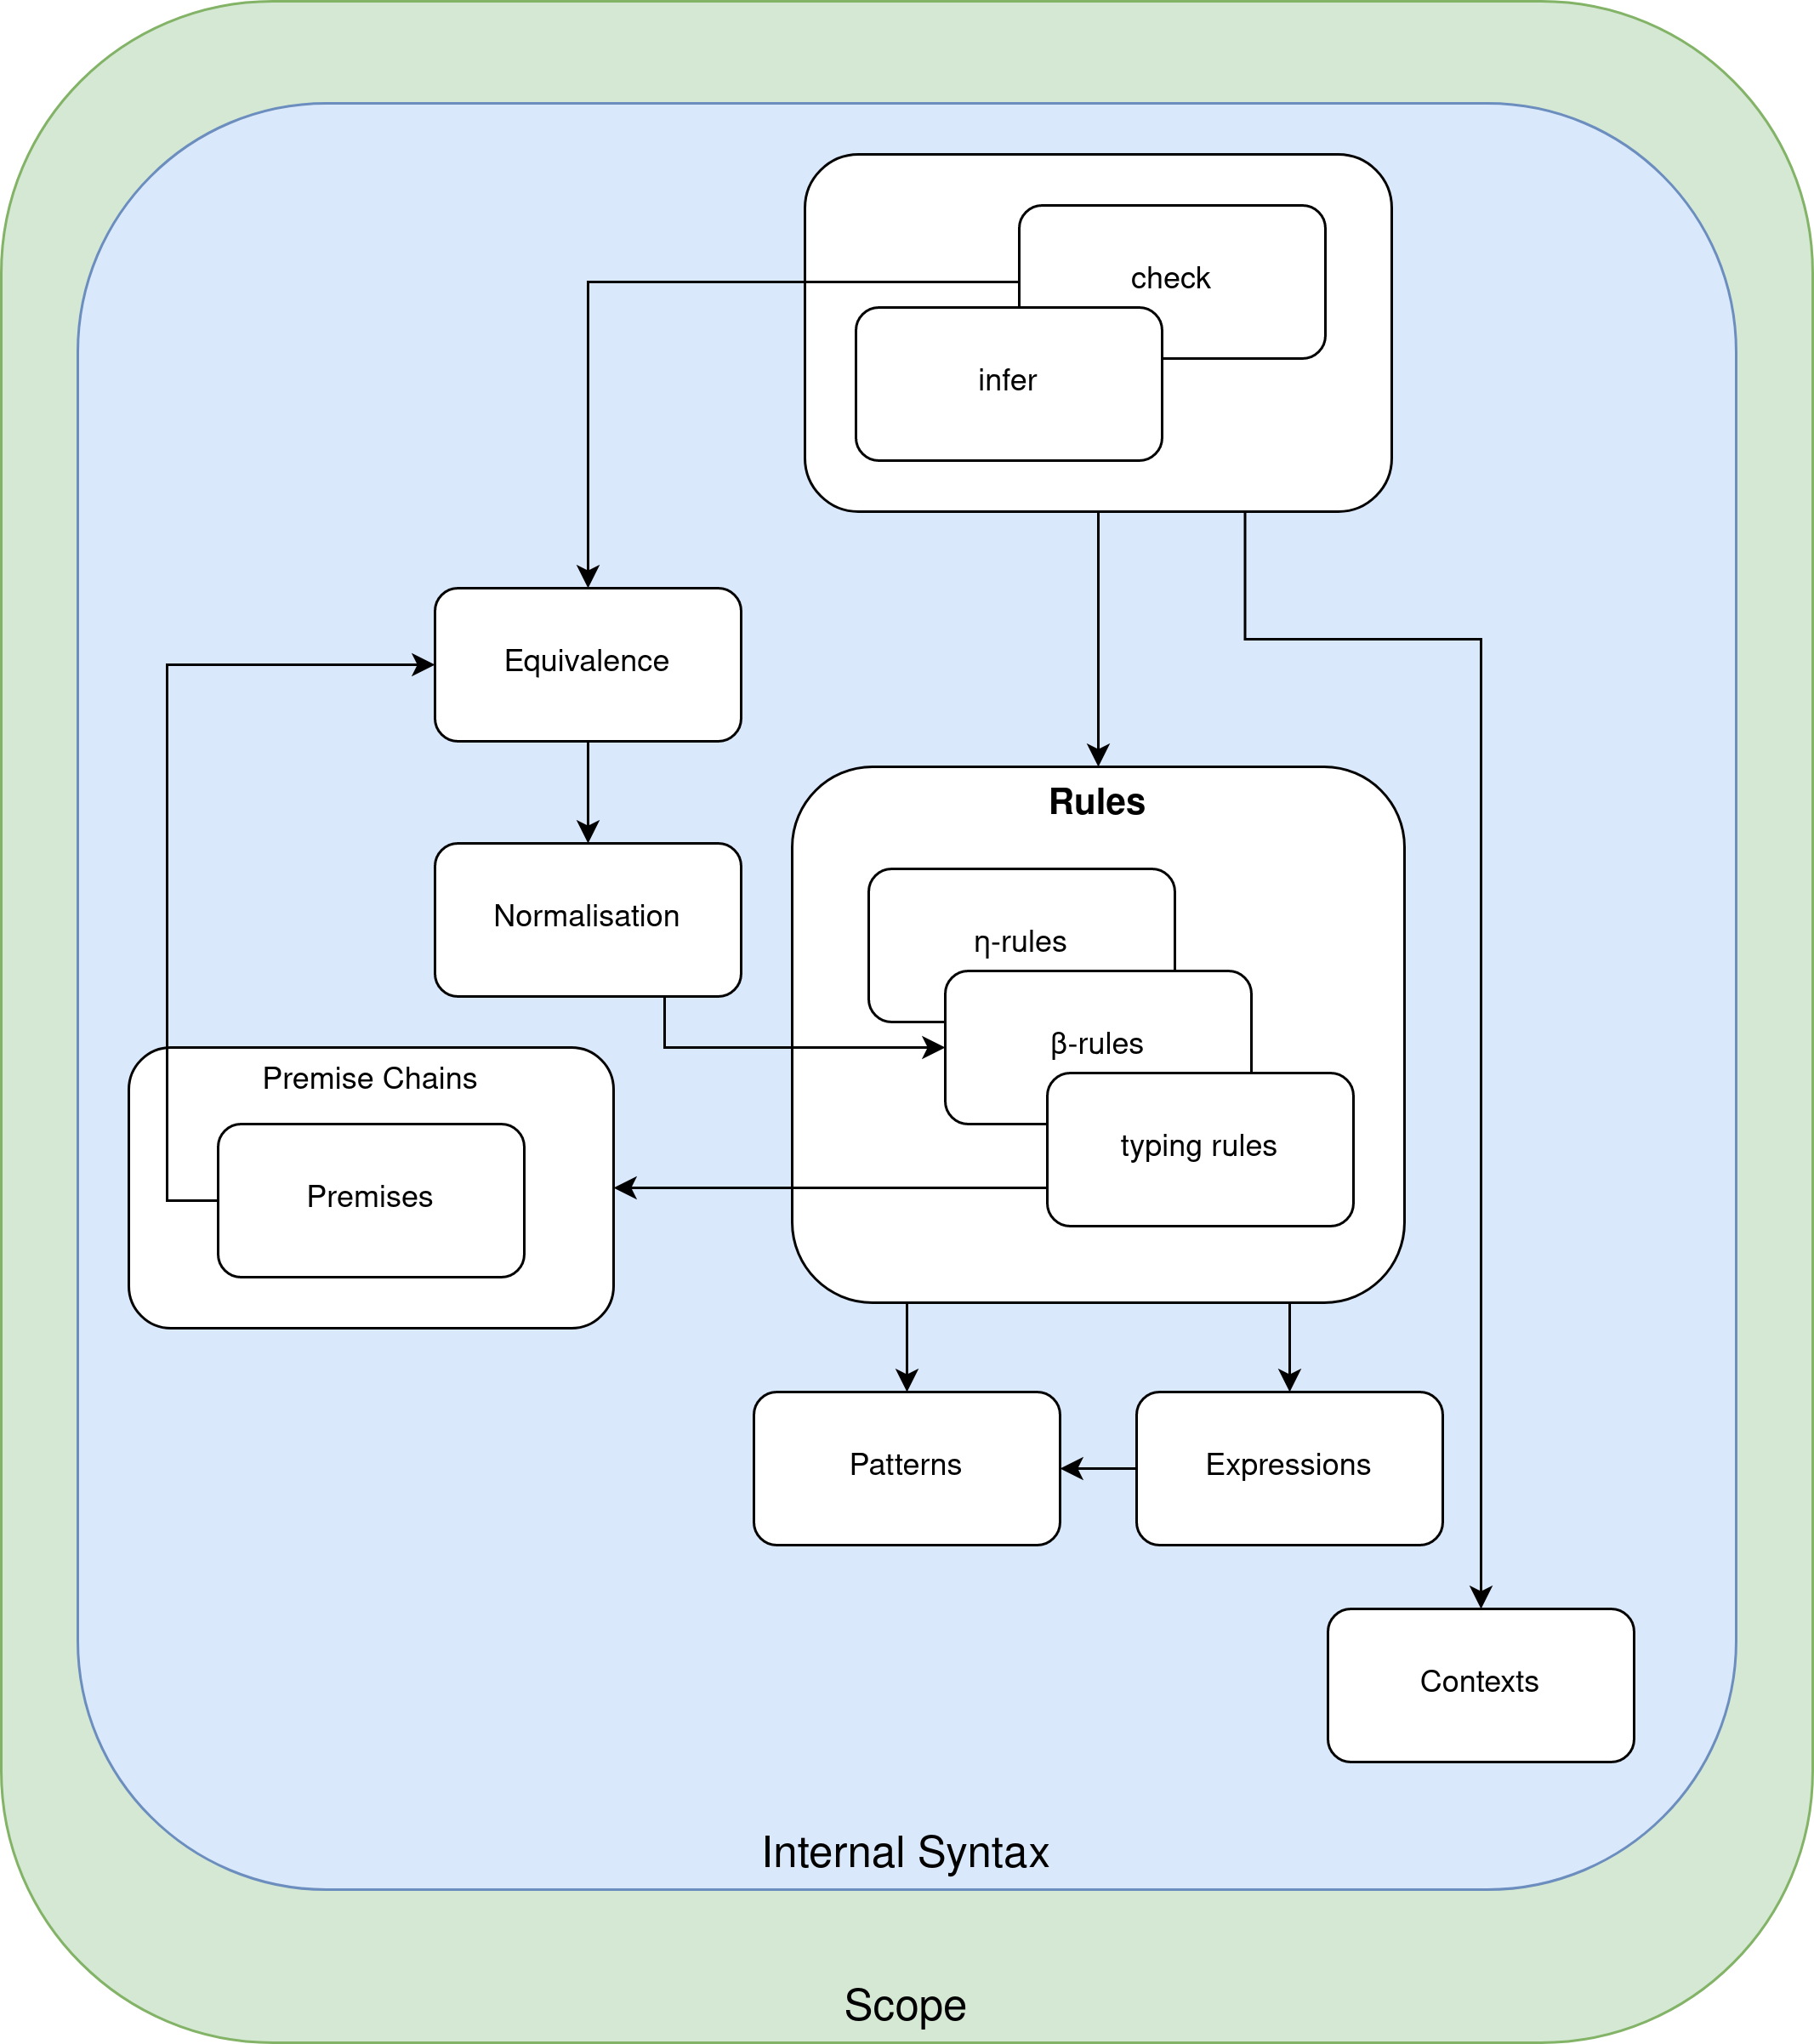
\includegraphics[width=\textwidth]{pictures/dependency-graph}
\end{figure}
\clearpage

\section{A core language}
\label{section-corelanguage}

\hide{
\begin{code}%
\>[0]\AgdaSymbol{\{-\#}\AgdaSpace{}%
\AgdaKeyword{OPTIONS}\AgdaSpace{}%
\AgdaPragma{--rewriting}\AgdaSpace{}%
\AgdaSymbol{\#-\}}\<%
\\
\>[0]\AgdaKeyword{module}\AgdaSpace{}%
\AgdaModule{CoreLanguage}\AgdaSpace{}%
\AgdaKeyword{where}\<%
\end{code}

\begin{code}%
\>[0]\AgdaKeyword{open}\AgdaSpace{}%
\AgdaKeyword{import}\AgdaSpace{}%
\AgdaModule{Data.Nat}\AgdaSpace{}%
\AgdaKeyword{using}\AgdaSpace{}%
\AgdaSymbol{(}\AgdaDatatype{ℕ}\AgdaSymbol{;}\AgdaSpace{}%
\AgdaInductiveConstructor{suc}\AgdaSymbol{;}\AgdaSpace{}%
\AgdaInductiveConstructor{zero}\AgdaSymbol{;}\AgdaSpace{}%
\AgdaOperator{\AgdaFunction{∣\AgdaUnderscore{}-\AgdaUnderscore{}∣}}\AgdaSymbol{)}\<%
\\
\>[0]\AgdaKeyword{open}\AgdaSpace{}%
\AgdaKeyword{import}\AgdaSpace{}%
\AgdaModule{Data.Nat.Show}\AgdaSpace{}%
\AgdaKeyword{using}\AgdaSpace{}%
\AgdaSymbol{(}\AgdaFunction{show}\AgdaSymbol{)}\<%
\\
\>[0]\AgdaKeyword{open}\AgdaSpace{}%
\AgdaKeyword{import}\AgdaSpace{}%
\AgdaModule{Data.String}\AgdaSpace{}%
\AgdaKeyword{using}\AgdaSpace{}%
\AgdaSymbol{(}\AgdaPostulate{String}\AgdaSymbol{;}\AgdaSpace{}%
\AgdaOperator{\AgdaFunction{\AgdaUnderscore{}++\AgdaUnderscore{}}}\AgdaSymbol{)}\<%
\\
\>[0]\AgdaKeyword{open}\AgdaSpace{}%
\AgdaKeyword{import}\AgdaSpace{}%
\AgdaModule{Function}\AgdaSpace{}%
\AgdaKeyword{using}\AgdaSpace{}%
\AgdaSymbol{(}\AgdaFunction{id}\AgdaSymbol{)}\<%
\end{code}
}

First, we introduce the concept of scope and what it means to be
scoped. In our system, all variables are de Bruijn indexed and our
scope can be represented by a single natural number. We take 0 to
mean nothing in scope, 1 to mean a single thing in scope and so on. A
scoped entity is one that is defined in terms of a scope.

\begin{code}%
\>[0]\AgdaFunction{Scope}%
\>[7]\AgdaSymbol{=}\AgdaSpace{}%
\AgdaDatatype{ℕ}\<%
\\
\>[0]\AgdaFunction{Scoped}\AgdaSpace{}%
\AgdaSymbol{=}\AgdaSpace{}%
\AgdaFunction{Scope}\AgdaSpace{}%
\AgdaSymbol{→}\AgdaSpace{}%
\AgdaPrimitiveType{Set}\<%
\end{code}

A variable is our first example of such a scoped entity which we
construct in order to maintain the invariant that a variable should
always refer to something in scope.

\hide{
\begin{code}%
\>[0]\AgdaKeyword{private}\<%
\\
\>[0][@{}l@{\AgdaIndent{0}}]%
\>[2]\AgdaKeyword{variable}\<%
\\
\>[2][@{}l@{\AgdaIndent{0}}]%
\>[4]\AgdaGeneralizable{γ}\AgdaSpace{}%
\AgdaSymbol{:}\AgdaSpace{}%
\AgdaFunction{Scope}\<%
\\
%
\>[4]\AgdaGeneralizable{δ}\AgdaSpace{}%
\AgdaSymbol{:}\AgdaSpace{}%
\AgdaFunction{Scope}\<%
\end{code}
}

\begin{code}%
\>[0]\AgdaKeyword{data}\AgdaSpace{}%
\AgdaDatatype{Var}\AgdaSpace{}%
\AgdaSymbol{:}\AgdaSpace{}%
\AgdaFunction{Scoped}\AgdaSpace{}%
\AgdaKeyword{where}\<%
\\
\>[0][@{}l@{\AgdaIndent{0}}]%
\>[2]\AgdaInductiveConstructor{ze}\AgdaSpace{}%
\AgdaSymbol{:}\AgdaSpace{}%
\AgdaDatatype{Var}\AgdaSpace{}%
\AgdaSymbol{(}\AgdaInductiveConstructor{suc}\AgdaSpace{}%
\AgdaGeneralizable{γ}\AgdaSymbol{)}\<%
\\
%
\>[2]\AgdaInductiveConstructor{su}\AgdaSpace{}%
\AgdaSymbol{:}\AgdaSpace{}%
\AgdaDatatype{Var}\AgdaSpace{}%
\AgdaGeneralizable{γ}\AgdaSpace{}%
\AgdaSymbol{→}\AgdaSpace{}%
\AgdaDatatype{Var}\AgdaSpace{}%
\AgdaSymbol{(}\AgdaInductiveConstructor{suc}\AgdaSpace{}%
\AgdaGeneralizable{γ}\AgdaSymbol{)}\<%
\end{code}

\hide{
\begin{code}%
\>[0]\AgdaFunction{toNum}\AgdaSpace{}%
\AgdaSymbol{:}\AgdaSpace{}%
\AgdaDatatype{Var}\AgdaSpace{}%
\AgdaGeneralizable{γ}\AgdaSpace{}%
\AgdaSymbol{→}\AgdaSpace{}%
\AgdaDatatype{ℕ}\<%
\\
\>[0]\AgdaFunction{toNum}\AgdaSpace{}%
\AgdaInductiveConstructor{ze}%
\>[13]\AgdaSymbol{=}\AgdaSpace{}%
\AgdaNumber{0}\<%
\\
\>[0]\AgdaFunction{toNum}\AgdaSpace{}%
\AgdaSymbol{(}\AgdaInductiveConstructor{su}\AgdaSpace{}%
\AgdaBound{v}\AgdaSymbol{)}\AgdaSpace{}%
\AgdaSymbol{=}\AgdaSpace{}%
\AgdaInductiveConstructor{suc}\AgdaSpace{}%
\AgdaSymbol{(}\AgdaFunction{toNum}\AgdaSpace{}%
\AgdaBound{v}\AgdaSymbol{)}\<%
\\
%
\\[\AgdaEmptyExtraSkip]%
\>[0]\AgdaFunction{fromNum}\AgdaSpace{}%
\AgdaSymbol{:}\AgdaSpace{}%
\AgdaSymbol{(}\AgdaBound{n}\AgdaSpace{}%
\AgdaSymbol{:}\AgdaSpace{}%
\AgdaDatatype{ℕ}\AgdaSymbol{)}\AgdaSpace{}%
\AgdaSymbol{→}\AgdaSpace{}%
\AgdaDatatype{Var}\AgdaSpace{}%
\AgdaSymbol{(}\AgdaInductiveConstructor{suc}\AgdaSpace{}%
\AgdaBound{n}\AgdaSymbol{)}\<%
\\
\>[0]\AgdaFunction{fromNum}\AgdaSpace{}%
\AgdaInductiveConstructor{zero}\AgdaSpace{}%
\AgdaSymbol{=}\AgdaSpace{}%
\AgdaInductiveConstructor{ze}\<%
\\
\>[0]\AgdaFunction{fromNum}\AgdaSpace{}%
\AgdaSymbol{(}\AgdaInductiveConstructor{suc}\AgdaSpace{}%
\AgdaBound{n}\AgdaSymbol{)}\AgdaSpace{}%
\AgdaSymbol{=}\AgdaSpace{}%
\AgdaInductiveConstructor{su}\AgdaSpace{}%
\AgdaSymbol{(}\AgdaFunction{fromNum}\AgdaSpace{}%
\AgdaBound{n}\AgdaSymbol{)}\<%
\end{code}
}


Our internal syntax is split into two broad grammatical
classes: constructions and computations. Constructions will have
their type checked, while computations have their type synthesized.

\hide{
\begin{code}%
\>[0]\AgdaKeyword{data}\AgdaSpace{}%
\AgdaDatatype{Const}\AgdaSpace{}%
\AgdaSymbol{(}\AgdaBound{γ}\AgdaSpace{}%
\AgdaSymbol{:}\AgdaSpace{}%
\AgdaFunction{Scope}\AgdaSymbol{)}\AgdaSpace{}%
\AgdaSymbol{:}\AgdaSpace{}%
\AgdaPrimitiveType{Set}\<%
\\
\>[0]\AgdaKeyword{data}\AgdaSpace{}%
\AgdaDatatype{Compu}\AgdaSpace{}%
\AgdaSymbol{(}\AgdaBound{γ}\AgdaSpace{}%
\AgdaSymbol{:}\AgdaSpace{}%
\AgdaFunction{Scope}\AgdaSymbol{)}\AgdaSpace{}%
\AgdaSymbol{:}\AgdaSpace{}%
\AgdaPrimitiveType{Set}\<%
\end{code}
}

\begin{code}%
\>[0]\AgdaKeyword{data}\AgdaSpace{}%
\AgdaDatatype{Const}\AgdaSpace{}%
\AgdaBound{γ}\AgdaSpace{}%
\AgdaKeyword{where}\<%
\\
\>[0][@{}l@{\AgdaIndent{0}}]%
\>[2]\AgdaInductiveConstructor{`}%
\>[9]\AgdaSymbol{:}\AgdaSpace{}%
\AgdaPostulate{String}\AgdaSpace{}%
\AgdaSymbol{→}\AgdaSpace{}%
\AgdaDatatype{Const}\AgdaSpace{}%
\AgdaBound{γ}\<%
\\
%
\>[2]\AgdaOperator{\AgdaInductiveConstructor{\AgdaUnderscore{}∙\AgdaUnderscore{}}}%
\>[9]\AgdaSymbol{:}\AgdaSpace{}%
\AgdaDatatype{Const}\AgdaSpace{}%
\AgdaBound{γ}\AgdaSpace{}%
\AgdaSymbol{→}\AgdaSpace{}%
\AgdaDatatype{Const}\AgdaSpace{}%
\AgdaBound{γ}\AgdaSpace{}%
\AgdaSymbol{→}\AgdaSpace{}%
\AgdaDatatype{Const}\AgdaSpace{}%
\AgdaBound{γ}\<%
\\
%
\>[2]\AgdaInductiveConstructor{bind}%
\>[9]\AgdaSymbol{:}\AgdaSpace{}%
\AgdaDatatype{Const}\AgdaSpace{}%
\AgdaSymbol{(}\AgdaInductiveConstructor{suc}\AgdaSpace{}%
\AgdaBound{γ}\AgdaSymbol{)}\AgdaSpace{}%
\AgdaSymbol{→}\AgdaSpace{}%
\AgdaDatatype{Const}\AgdaSpace{}%
\AgdaBound{γ}\<%
\\
%
\>[2]\AgdaInductiveConstructor{thunk}%
\>[9]\AgdaSymbol{:}\AgdaSpace{}%
\AgdaDatatype{Compu}\AgdaSpace{}%
\AgdaBound{γ}\AgdaSpace{}%
\AgdaSymbol{→}\AgdaSpace{}%
\AgdaDatatype{Const}\AgdaSpace{}%
\AgdaBound{γ}\<%
\\
%
\\[\AgdaEmptyExtraSkip]%
\>[0]\AgdaKeyword{data}\AgdaSpace{}%
\AgdaDatatype{Compu}\AgdaSpace{}%
\AgdaBound{γ}\AgdaSpace{}%
\AgdaKeyword{where}\<%
\\
\>[0][@{}l@{\AgdaIndent{0}}]%
\>[2]\AgdaInductiveConstructor{var}%
\>[9]\AgdaSymbol{:}\AgdaSpace{}%
\AgdaDatatype{Var}\AgdaSpace{}%
\AgdaBound{γ}\AgdaSpace{}%
\AgdaSymbol{→}\AgdaSpace{}%
\AgdaDatatype{Compu}\AgdaSpace{}%
\AgdaBound{γ}\<%
\\
%
\>[2]\AgdaInductiveConstructor{elim}%
\>[9]\AgdaSymbol{:}\AgdaSpace{}%
\AgdaDatatype{Compu}\AgdaSpace{}%
\AgdaBound{γ}\AgdaSpace{}%
\AgdaSymbol{→}\AgdaSpace{}%
\AgdaDatatype{Const}\AgdaSpace{}%
\AgdaBound{γ}\AgdaSpace{}%
\AgdaSymbol{→}\AgdaSpace{}%
\AgdaDatatype{Compu}\AgdaSpace{}%
\AgdaBound{γ}\<%
\\
%
\>[2]\AgdaOperator{\AgdaInductiveConstructor{\AgdaUnderscore{}∷\AgdaUnderscore{}}}%
\>[9]\AgdaSymbol{:}\AgdaSpace{}%
\AgdaDatatype{Const}\AgdaSpace{}%
\AgdaBound{γ}\AgdaSpace{}%
\AgdaSymbol{→}\AgdaSpace{}%
\AgdaDatatype{Const}\AgdaSpace{}%
\AgdaBound{γ}\AgdaSpace{}%
\AgdaSymbol{→}\AgdaSpace{}%
\AgdaDatatype{Compu}\AgdaSpace{}%
\AgdaBound{γ}\<%
\\
%
\\[\AgdaEmptyExtraSkip]%
\>[0]\AgdaKeyword{data}\AgdaSpace{}%
\AgdaDatatype{Dir}\AgdaSpace{}%
\AgdaSymbol{:}\AgdaSpace{}%
\AgdaPrimitiveType{Set}\AgdaSpace{}%
\AgdaKeyword{where}\AgdaSpace{}%
\AgdaInductiveConstructor{const}\AgdaSpace{}%
\AgdaInductiveConstructor{compu}\AgdaSpace{}%
\AgdaSymbol{:}\AgdaSpace{}%
\AgdaDatatype{Dir}\<%
\\
%
\\[\AgdaEmptyExtraSkip]%
\>[0]\AgdaFunction{Term}\AgdaSpace{}%
\AgdaSymbol{:}\AgdaSpace{}%
\AgdaDatatype{Dir}\AgdaSpace{}%
\AgdaSymbol{→}\AgdaSpace{}%
\AgdaFunction{Scoped}\<%
\\
\>[0]\AgdaFunction{Term}\AgdaSpace{}%
\AgdaInductiveConstructor{const}%
\>[12]\AgdaSymbol{=}\AgdaSpace{}%
\AgdaDatatype{Const}\<%
\\
\>[0]\AgdaFunction{Term}\AgdaSpace{}%
\AgdaInductiveConstructor{compu}%
\>[12]\AgdaSymbol{=}\AgdaSpace{}%
\AgdaDatatype{Compu}\<%
\end{code}

This syntax gives us the means to represent atoms of original syntax
with `, pairs of syntax elements, binding sites (thus increasing the scope
for a subterm), variables, type annotated terms with "::" and eliminations
- the sites of $β$-reductions. We are also able to embed computations into
constructions using thunk, as being able to synthesize the type of a term
guarantees that we are able to check it.

Note that blindly embedding synthesizable terms with a thunk is
not always the best course of action. In the case of an annotated
term, we already have a suitable construction under the annotation.
For convenience, we provide a function to perform this embedding and
hence a function to take \emph{any} computation to a construction and
another to take any term to a construction. We also prove the opposite
functionality, allowing us to take any term to a computation, however in
this case we need to supply a construction that we claim to be the type.
This may or may not be used in constructing the computation.

\hide{
\begin{code}%
\>[0]\AgdaKeyword{private}\<%
\\
\>[0][@{}l@{\AgdaIndent{0}}]%
\>[2]\AgdaKeyword{variable}\<%
\\
\>[2][@{}l@{\AgdaIndent{0}}]%
\>[4]\AgdaGeneralizable{d}\AgdaSpace{}%
\AgdaSymbol{:}\AgdaSpace{}%
\AgdaDatatype{Dir}\<%
\end{code}
}
\begin{code}%
\>[0]\AgdaFunction{↠}\AgdaSpace{}%
\AgdaSymbol{:}\AgdaSpace{}%
\AgdaDatatype{Compu}\AgdaSpace{}%
\AgdaGeneralizable{γ}\AgdaSpace{}%
\AgdaSymbol{→}\AgdaSpace{}%
\AgdaDatatype{Const}\AgdaSpace{}%
\AgdaGeneralizable{γ}\<%
\\
\>[0]\AgdaFunction{↠}\AgdaSpace{}%
\AgdaSymbol{(}\AgdaBound{t}\AgdaSpace{}%
\AgdaOperator{\AgdaInductiveConstructor{∷}}\AgdaSpace{}%
\AgdaBound{T}\AgdaSymbol{)}\AgdaSpace{}%
\AgdaSymbol{=}\AgdaSpace{}%
\AgdaBound{t}\<%
\\
\>[0]\AgdaCatchallClause{\AgdaFunction{↠}}%
\>[3]\AgdaCatchallClause{\AgdaBound{x}}%
\>[10]\AgdaSymbol{=}\AgdaSpace{}%
\AgdaInductiveConstructor{thunk}\AgdaSpace{}%
\AgdaBound{x}\<%
\\
%
\\[\AgdaEmptyExtraSkip]%
\>[0]\AgdaFunction{↠↠}\AgdaSpace{}%
\AgdaSymbol{:}\AgdaSpace{}%
\AgdaFunction{Term}\AgdaSpace{}%
\AgdaGeneralizable{d}\AgdaSpace{}%
\AgdaGeneralizable{γ}\AgdaSpace{}%
\AgdaSymbol{→}\AgdaSpace{}%
\AgdaDatatype{Const}\AgdaSpace{}%
\AgdaGeneralizable{γ}\<%
\\
\>[0]\AgdaFunction{↠↠}\AgdaSpace{}%
\AgdaSymbol{\{}\AgdaInductiveConstructor{const}\AgdaSymbol{\}}\AgdaSpace{}%
\AgdaSymbol{=}\AgdaSpace{}%
\AgdaFunction{id}\<%
\\
\>[0]\AgdaFunction{↠↠}\AgdaSpace{}%
\AgdaSymbol{\{}\AgdaInductiveConstructor{compu}\AgdaSymbol{\}}\AgdaSpace{}%
\AgdaSymbol{=}\AgdaSpace{}%
\AgdaFunction{↠}\<%
\\
%
\\[\AgdaEmptyExtraSkip]%
\>[0]\AgdaFunction{↞↞}\AgdaSpace{}%
\AgdaSymbol{:}\AgdaSpace{}%
\AgdaFunction{Term}\AgdaSpace{}%
\AgdaGeneralizable{d}\AgdaSpace{}%
\AgdaGeneralizable{γ}\AgdaSpace{}%
\AgdaSymbol{→}\AgdaSpace{}%
\AgdaDatatype{Const}\AgdaSpace{}%
\AgdaGeneralizable{γ}\AgdaSpace{}%
\AgdaSymbol{→}\AgdaSpace{}%
\AgdaDatatype{Compu}\AgdaSpace{}%
\AgdaGeneralizable{γ}\<%
\\
\>[0]\AgdaFunction{↞↞}\AgdaSpace{}%
\AgdaSymbol{\{}\AgdaInductiveConstructor{const}\AgdaSymbol{\}}\AgdaSpace{}%
\AgdaSymbol{(}\AgdaInductiveConstructor{thunk}\AgdaSpace{}%
\AgdaBound{x}\AgdaSymbol{)}\AgdaSpace{}%
\AgdaBound{T}%
\>[24]\AgdaSymbol{=}\AgdaSpace{}%
\AgdaBound{x}\<%
\\
\>[0]\AgdaCatchallClause{\AgdaFunction{↞↞}}\AgdaSpace{}%
\AgdaCatchallClause{\AgdaSymbol{\{}}\AgdaCatchallClause{\AgdaInductiveConstructor{const}}\AgdaCatchallClause{\AgdaSymbol{\}}}%
\>[12]\AgdaCatchallClause{\AgdaBound{t}}%
\>[21]\AgdaCatchallClause{\AgdaBound{T}}%
\>[24]\AgdaSymbol{=}\AgdaSpace{}%
\AgdaBound{t}\AgdaSpace{}%
\AgdaOperator{\AgdaInductiveConstructor{∷}}\AgdaSpace{}%
\AgdaBound{T}\<%
\\
\>[0]\AgdaFunction{↞↞}\AgdaSpace{}%
\AgdaSymbol{\{}\AgdaInductiveConstructor{compu}\AgdaSymbol{\}}%
\>[12]\AgdaBound{t}%
\>[21]\AgdaSymbol{\AgdaUnderscore{}}%
\>[24]\AgdaSymbol{=}\AgdaSpace{}%
\AgdaBound{t}\<%
\end{code}

\hide{
\begin{code}%
\>[0]\AgdaKeyword{infixr}\AgdaSpace{}%
\AgdaNumber{20}\AgdaSpace{}%
\AgdaOperator{\AgdaInductiveConstructor{\AgdaUnderscore{}∙\AgdaUnderscore{}}}\<%
\\
%
\\[\AgdaEmptyExtraSkip]%
\>[0]\AgdaFunction{print}\AgdaSpace{}%
\AgdaSymbol{:}\AgdaSpace{}%
\AgdaFunction{Term}\AgdaSpace{}%
\AgdaGeneralizable{d}\AgdaSpace{}%
\AgdaGeneralizable{γ}\AgdaSpace{}%
\AgdaSymbol{→}\AgdaSpace{}%
\AgdaPostulate{String}\<%
\\
\>[0]\AgdaFunction{print}\AgdaSpace{}%
\AgdaSymbol{\{}\AgdaInductiveConstructor{const}\AgdaSymbol{\}}\AgdaSpace{}%
\AgdaSymbol{(}\AgdaInductiveConstructor{`}\AgdaSpace{}%
\AgdaBound{x}\AgdaSymbol{)}%
\>[25]\AgdaSymbol{=}\AgdaSpace{}%
\AgdaBound{x}\<%
\\
\>[0]\AgdaFunction{print}\AgdaSpace{}%
\AgdaSymbol{\{}\AgdaInductiveConstructor{const}\AgdaSymbol{\}}\AgdaSpace{}%
\AgdaSymbol{(}\AgdaInductiveConstructor{`}\AgdaSpace{}%
\AgdaBound{x}\AgdaSpace{}%
\AgdaOperator{\AgdaInductiveConstructor{∙}}\AgdaSpace{}%
\AgdaBound{t}\AgdaSymbol{)}%
\>[25]\AgdaSymbol{=}\AgdaSpace{}%
\AgdaFunction{print}\AgdaSpace{}%
\AgdaSymbol{\{}\AgdaArgument{γ}\AgdaSpace{}%
\AgdaSymbol{=}\AgdaSpace{}%
\AgdaNumber{0}\AgdaSymbol{\}}\AgdaSpace{}%
\AgdaSymbol{(}\AgdaInductiveConstructor{`}\AgdaSpace{}%
\AgdaBound{x}\AgdaSymbol{)}\AgdaSpace{}%
\AgdaOperator{\AgdaFunction{++}}\AgdaSpace{}%
\AgdaString{" "}\AgdaSpace{}%
\AgdaOperator{\AgdaFunction{++}}\AgdaSpace{}%
\AgdaFunction{print}\AgdaSpace{}%
\AgdaBound{t}\<%
\\
\>[0]\AgdaCatchallClause{\AgdaFunction{print}}\AgdaSpace{}%
\AgdaCatchallClause{\AgdaSymbol{\{}}\AgdaCatchallClause{\AgdaInductiveConstructor{const}}\AgdaCatchallClause{\AgdaSymbol{\}}}\AgdaSpace{}%
\AgdaCatchallClause{\AgdaSymbol{(}}\AgdaCatchallClause{\AgdaBound{s}}\AgdaSpace{}%
\AgdaCatchallClause{\AgdaOperator{\AgdaInductiveConstructor{∙}}}\AgdaSpace{}%
\AgdaCatchallClause{\AgdaBound{t}}\AgdaCatchallClause{\AgdaSymbol{)}}%
\>[25]\AgdaSymbol{=}\AgdaSpace{}%
\AgdaString{"("}\AgdaSpace{}%
\AgdaOperator{\AgdaFunction{++}}\AgdaSpace{}%
\AgdaFunction{print}\AgdaSpace{}%
\AgdaBound{s}\AgdaSpace{}%
\AgdaOperator{\AgdaFunction{++}}\AgdaSpace{}%
\AgdaString{") "}\AgdaSpace{}%
\AgdaOperator{\AgdaFunction{++}}\AgdaSpace{}%
\AgdaFunction{print}\AgdaSpace{}%
\AgdaBound{t}\<%
\\
\>[0]\AgdaFunction{print}\AgdaSpace{}%
\AgdaSymbol{\{}\AgdaInductiveConstructor{const}\AgdaSymbol{\}}\AgdaSpace{}%
\AgdaSymbol{\{}\AgdaBound{γ}\AgdaSymbol{\}}\AgdaSpace{}%
\AgdaSymbol{(}\AgdaInductiveConstructor{bind}\AgdaSpace{}%
\AgdaBound{x}\AgdaSymbol{)}%
\>[29]\AgdaSymbol{=}\AgdaSpace{}%
\AgdaString{"V"}\AgdaSpace{}%
\AgdaOperator{\AgdaFunction{++}}\AgdaSpace{}%
\AgdaFunction{show}\AgdaSpace{}%
\AgdaBound{γ}\AgdaSpace{}%
\AgdaOperator{\AgdaFunction{++}}\AgdaSpace{}%
\AgdaString{" "}\AgdaSpace{}%
\AgdaOperator{\AgdaFunction{++}}\AgdaSpace{}%
\AgdaFunction{print}\AgdaSpace{}%
\AgdaBound{x}\<%
\\
\>[0]\AgdaFunction{print}\AgdaSpace{}%
\AgdaSymbol{\{}\AgdaInductiveConstructor{const}\AgdaSymbol{\}}\AgdaSpace{}%
\AgdaSymbol{(}\AgdaInductiveConstructor{thunk}\AgdaSpace{}%
\AgdaBound{x}\AgdaSymbol{)}%
\>[25]\AgdaSymbol{=}\AgdaSpace{}%
\AgdaFunction{print}\AgdaSpace{}%
\AgdaBound{x}\<%
\\
\>[0]\AgdaFunction{print}\AgdaSpace{}%
\AgdaSymbol{\{}\AgdaInductiveConstructor{compu}\AgdaSymbol{\}}\AgdaSpace{}%
\AgdaSymbol{\{}\AgdaBound{γ}\AgdaSymbol{\}}\AgdaSpace{}%
\AgdaSymbol{(}\AgdaInductiveConstructor{var}\AgdaSpace{}%
\AgdaBound{x}\AgdaSymbol{)}%
\>[29]\AgdaSymbol{=}\AgdaSpace{}%
\AgdaString{"V"}\AgdaSpace{}%
\AgdaOperator{\AgdaFunction{++}}\AgdaSpace{}%
\AgdaFunction{show}\AgdaSpace{}%
\AgdaSymbol{(}\AgdaOperator{\AgdaFunction{∣}}\AgdaSpace{}%
\AgdaBound{γ}\AgdaSpace{}%
\AgdaOperator{\AgdaFunction{-}}\AgdaSpace{}%
\AgdaInductiveConstructor{suc}\AgdaSpace{}%
\AgdaSymbol{(}\AgdaFunction{toNum}\AgdaSpace{}%
\AgdaBound{x}\AgdaSymbol{)}\AgdaSpace{}%
\AgdaOperator{\AgdaFunction{∣}}\AgdaSymbol{)}\<%
\\
\>[0]\AgdaFunction{print}\AgdaSpace{}%
\AgdaSymbol{\{}\AgdaInductiveConstructor{compu}\AgdaSymbol{\}}\AgdaSpace{}%
\AgdaSymbol{(}\AgdaInductiveConstructor{elim}\AgdaSpace{}%
\AgdaBound{e}\AgdaSpace{}%
\AgdaBound{s}\AgdaSymbol{)}\AgdaSpace{}%
\AgdaSymbol{=}\AgdaSpace{}%
\AgdaString{"(elim "}\AgdaSpace{}%
\AgdaOperator{\AgdaFunction{++}}\AgdaSpace{}%
\AgdaFunction{print}\AgdaSpace{}%
\AgdaBound{e}\AgdaSpace{}%
\AgdaOperator{\AgdaFunction{++}}\AgdaSpace{}%
\AgdaString{" "}\AgdaSpace{}%
\AgdaOperator{\AgdaFunction{++}}\AgdaSpace{}%
\AgdaFunction{print}\AgdaSpace{}%
\AgdaBound{s}\AgdaSpace{}%
\AgdaOperator{\AgdaFunction{++}}\AgdaSpace{}%
\AgdaString{")"}\<%
\\
\>[0]\AgdaFunction{print}\AgdaSpace{}%
\AgdaSymbol{\{}\AgdaInductiveConstructor{compu}\AgdaSymbol{\}}\AgdaSpace{}%
\AgdaSymbol{(}\AgdaBound{t}\AgdaSpace{}%
\AgdaOperator{\AgdaInductiveConstructor{∷}}\AgdaSpace{}%
\AgdaBound{T}\AgdaSymbol{)}%
\>[25]\AgdaSymbol{=}\AgdaSpace{}%
\AgdaString{"("}\AgdaSpace{}%
\AgdaOperator{\AgdaFunction{++}}\AgdaSpace{}%
\AgdaFunction{print}\AgdaSpace{}%
\AgdaBound{t}\AgdaSpace{}%
\AgdaOperator{\AgdaFunction{++}}\AgdaSpace{}%
\AgdaString{" ∶ "}\AgdaSpace{}%
\AgdaOperator{\AgdaFunction{++}}\AgdaSpace{}%
\AgdaFunction{print}\AgdaSpace{}%
\AgdaBound{T}\AgdaSpace{}%
\AgdaOperator{\AgdaFunction{++}}\AgdaSpace{}%
\AgdaString{")"}\<%
\\
%
\\[\AgdaEmptyExtraSkip]%
\>[0]\AgdaFunction{printrawvar}\AgdaSpace{}%
\AgdaSymbol{:}\AgdaSpace{}%
\AgdaDatatype{Var}\AgdaSpace{}%
\AgdaGeneralizable{γ}\AgdaSpace{}%
\AgdaSymbol{→}\AgdaSpace{}%
\AgdaPostulate{String}\<%
\\
\>[0]\AgdaFunction{printrawvar}\AgdaSpace{}%
\AgdaInductiveConstructor{ze}%
\>[19]\AgdaSymbol{=}\AgdaSpace{}%
\AgdaString{"ze"}\<%
\\
\>[0]\AgdaFunction{printrawvar}\AgdaSpace{}%
\AgdaSymbol{(}\AgdaInductiveConstructor{su}\AgdaSpace{}%
\AgdaBound{v}\AgdaSymbol{)}\AgdaSpace{}%
\AgdaSymbol{=}\AgdaSpace{}%
\AgdaString{"su "}\AgdaSpace{}%
\AgdaOperator{\AgdaFunction{++}}\AgdaSpace{}%
\AgdaFunction{printrawvar}\AgdaSpace{}%
\AgdaBound{v}\<%
\\
%
\\[\AgdaEmptyExtraSkip]%
\>[0]\AgdaFunction{printraw}\AgdaSpace{}%
\AgdaSymbol{:}\AgdaSpace{}%
\AgdaFunction{Term}\AgdaSpace{}%
\AgdaGeneralizable{d}\AgdaSpace{}%
\AgdaGeneralizable{γ}\AgdaSpace{}%
\AgdaSymbol{→}\AgdaSpace{}%
\AgdaPostulate{String}\<%
\\
\>[0]\AgdaFunction{printraw}\AgdaSpace{}%
\AgdaSymbol{\{}\AgdaInductiveConstructor{const}\AgdaSymbol{\}}\AgdaSpace{}%
\AgdaSymbol{(}\AgdaInductiveConstructor{`}\AgdaSpace{}%
\AgdaBound{x}\AgdaSymbol{)}%
\>[29]\AgdaSymbol{=}\AgdaSpace{}%
\AgdaString{"(` '"}\AgdaSpace{}%
\AgdaOperator{\AgdaFunction{++}}\AgdaSpace{}%
\AgdaBound{x}\AgdaSpace{}%
\AgdaOperator{\AgdaFunction{++}}\AgdaSpace{}%
\AgdaString{"')"}\<%
\\
\>[0]\AgdaFunction{printraw}\AgdaSpace{}%
\AgdaSymbol{\{}\AgdaInductiveConstructor{const}\AgdaSymbol{\}}\AgdaSpace{}%
\AgdaSymbol{(}\AgdaBound{s}\AgdaSpace{}%
\AgdaOperator{\AgdaInductiveConstructor{∙}}\AgdaSpace{}%
\AgdaBound{t}\AgdaSymbol{)}%
\>[29]\AgdaSymbol{=}\AgdaSpace{}%
\AgdaString{"("}\AgdaSpace{}%
\AgdaOperator{\AgdaFunction{++}}\AgdaSpace{}%
\AgdaFunction{printraw}\AgdaSpace{}%
\AgdaBound{s}\AgdaSpace{}%
\AgdaOperator{\AgdaFunction{++}}\AgdaSpace{}%
\AgdaString{" ∙ "}%
\>[59]\AgdaOperator{\AgdaFunction{++}}\AgdaSpace{}%
\AgdaFunction{printraw}\AgdaSpace{}%
\AgdaBound{t}\AgdaSpace{}%
\AgdaOperator{\AgdaFunction{++}}\AgdaSpace{}%
\AgdaString{")"}\<%
\\
\>[0]\AgdaFunction{printraw}\AgdaSpace{}%
\AgdaSymbol{\{}\AgdaInductiveConstructor{const}\AgdaSymbol{\}}\AgdaSpace{}%
\AgdaSymbol{\{}\AgdaBound{γ}\AgdaSymbol{\}}\AgdaSpace{}%
\AgdaSymbol{(}\AgdaInductiveConstructor{bind}\AgdaSpace{}%
\AgdaBound{x}\AgdaSymbol{)}%
\>[33]\AgdaSymbol{=}\AgdaSpace{}%
\AgdaString{"("}\AgdaSpace{}%
\AgdaOperator{\AgdaFunction{++}}\AgdaSpace{}%
\AgdaString{"V"}\AgdaSpace{}%
\AgdaOperator{\AgdaFunction{++}}\AgdaSpace{}%
\AgdaFunction{show}\AgdaSpace{}%
\AgdaSymbol{(}\AgdaInductiveConstructor{suc}\AgdaSpace{}%
\AgdaBound{γ}\AgdaSymbol{)}\AgdaSpace{}%
\AgdaOperator{\AgdaFunction{++}}\AgdaSpace{}%
\AgdaString{" "}\AgdaSpace{}%
\AgdaOperator{\AgdaFunction{++}}\AgdaSpace{}%
\AgdaFunction{printraw}\AgdaSpace{}%
\AgdaBound{x}\AgdaSpace{}%
\AgdaOperator{\AgdaFunction{++}}\AgdaSpace{}%
\AgdaString{")"}\<%
\\
\>[0]\AgdaFunction{printraw}\AgdaSpace{}%
\AgdaSymbol{\{}\AgdaInductiveConstructor{const}\AgdaSymbol{\}}\AgdaSpace{}%
\AgdaSymbol{(}\AgdaInductiveConstructor{thunk}\AgdaSpace{}%
\AgdaBound{x}\AgdaSymbol{)}%
\>[29]\AgdaSymbol{=}\AgdaSpace{}%
\AgdaString{"(thunk "}\AgdaSpace{}%
\AgdaOperator{\AgdaFunction{++}}\AgdaSpace{}%
\AgdaFunction{printraw}\AgdaSpace{}%
\AgdaBound{x}\AgdaSpace{}%
\AgdaOperator{\AgdaFunction{++}}\AgdaSpace{}%
\AgdaString{")"}\<%
\\
\>[0]\AgdaFunction{printraw}\AgdaSpace{}%
\AgdaSymbol{\{}\AgdaInductiveConstructor{compu}\AgdaSymbol{\}}\AgdaSpace{}%
\AgdaSymbol{(}\AgdaInductiveConstructor{var}\AgdaSpace{}%
\AgdaBound{x}\AgdaSymbol{)}%
\>[29]\AgdaSymbol{=}\AgdaSpace{}%
\AgdaString{"(var "}\AgdaSpace{}%
\AgdaOperator{\AgdaFunction{++}}\AgdaSpace{}%
\AgdaFunction{printrawvar}\AgdaSpace{}%
\AgdaBound{x}\AgdaSpace{}%
\AgdaOperator{\AgdaFunction{++}}\AgdaSpace{}%
\AgdaString{")"}\<%
\\
\>[0]\AgdaFunction{printraw}\AgdaSpace{}%
\AgdaSymbol{\{}\AgdaInductiveConstructor{compu}\AgdaSymbol{\}}\AgdaSpace{}%
\AgdaSymbol{(}\AgdaInductiveConstructor{elim}\AgdaSpace{}%
\AgdaBound{e}\AgdaSpace{}%
\AgdaBound{s}\AgdaSymbol{)}%
\>[29]\AgdaSymbol{=}\AgdaSpace{}%
\AgdaString{"(elim "}\AgdaSpace{}%
\AgdaOperator{\AgdaFunction{++}}\AgdaSpace{}%
\AgdaFunction{printraw}\AgdaSpace{}%
\AgdaBound{e}\AgdaSpace{}%
\AgdaOperator{\AgdaFunction{++}}\AgdaSpace{}%
\AgdaString{" "}\AgdaSpace{}%
\AgdaOperator{\AgdaFunction{++}}\AgdaSpace{}%
\AgdaFunction{printraw}\AgdaSpace{}%
\AgdaBound{s}\AgdaSpace{}%
\AgdaOperator{\AgdaFunction{++}}\AgdaSpace{}%
\AgdaString{")"}\<%
\\
\>[0]\AgdaFunction{printraw}\AgdaSpace{}%
\AgdaSymbol{\{}\AgdaInductiveConstructor{compu}\AgdaSymbol{\}}\AgdaSpace{}%
\AgdaSymbol{(}\AgdaBound{t}\AgdaSpace{}%
\AgdaOperator{\AgdaInductiveConstructor{∷}}\AgdaSpace{}%
\AgdaBound{T}\AgdaSymbol{)}%
\>[29]\AgdaSymbol{=}\AgdaSpace{}%
\AgdaString{"("}\AgdaSpace{}%
\AgdaOperator{\AgdaFunction{++}}\AgdaSpace{}%
\AgdaFunction{printraw}\AgdaSpace{}%
\AgdaBound{t}\AgdaSpace{}%
\AgdaOperator{\AgdaFunction{++}}\AgdaSpace{}%
\AgdaString{"∶"}\AgdaSpace{}%
\AgdaOperator{\AgdaFunction{++}}\AgdaSpace{}%
\AgdaFunction{printraw}\AgdaSpace{}%
\AgdaBound{T}\AgdaSpace{}%
\AgdaOperator{\AgdaFunction{++}}\AgdaSpace{}%
\AgdaString{")"}\<%
\\
%
\\[\AgdaEmptyExtraSkip]%
\>[0]\AgdaOperator{\AgdaFunction{\AgdaUnderscore{}<<\AgdaUnderscore{}}}\AgdaSpace{}%
\AgdaSymbol{:}\AgdaSpace{}%
\AgdaDatatype{Const}\AgdaSpace{}%
\AgdaGeneralizable{γ}\AgdaSpace{}%
\AgdaSymbol{→}\AgdaSpace{}%
\AgdaDatatype{Const}\AgdaSpace{}%
\AgdaGeneralizable{γ}\AgdaSpace{}%
\AgdaSymbol{→}\AgdaSpace{}%
\AgdaDatatype{Const}\AgdaSpace{}%
\AgdaGeneralizable{γ}\<%
\\
\>[0]\AgdaInductiveConstructor{`}\AgdaSpace{}%
\AgdaBound{x}\AgdaSpace{}%
\AgdaOperator{\AgdaFunction{<<}}\AgdaSpace{}%
\AgdaBound{y}%
\>[15]\AgdaSymbol{=}\AgdaSpace{}%
\AgdaInductiveConstructor{`}\AgdaSpace{}%
\AgdaBound{x}\AgdaSpace{}%
\AgdaOperator{\AgdaInductiveConstructor{∙}}\AgdaSpace{}%
\AgdaBound{y}\<%
\\
\>[0]\AgdaSymbol{(}\AgdaBound{x}\AgdaSpace{}%
\AgdaOperator{\AgdaInductiveConstructor{∙}}\AgdaSpace{}%
\AgdaBound{y'}\AgdaSymbol{)}\AgdaSpace{}%
\AgdaOperator{\AgdaFunction{<<}}\AgdaSpace{}%
\AgdaBound{y}%
\>[15]\AgdaSymbol{=}\AgdaSpace{}%
\AgdaBound{x}\AgdaSpace{}%
\AgdaOperator{\AgdaInductiveConstructor{∙}}\AgdaSpace{}%
\AgdaSymbol{(}\AgdaBound{y'}\AgdaSpace{}%
\AgdaOperator{\AgdaFunction{<<}}\AgdaSpace{}%
\AgdaBound{y}\AgdaSymbol{)}\<%
\\
\>[0]\AgdaInductiveConstructor{bind}\AgdaSpace{}%
\AgdaBound{x}\AgdaSpace{}%
\AgdaOperator{\AgdaFunction{<<}}\AgdaSpace{}%
\AgdaBound{y}%
\>[15]\AgdaSymbol{=}\AgdaSpace{}%
\AgdaInductiveConstructor{bind}\AgdaSpace{}%
\AgdaBound{x}\AgdaSpace{}%
\AgdaOperator{\AgdaInductiveConstructor{∙}}\AgdaSpace{}%
\AgdaBound{y}\<%
\\
\>[0]\AgdaInductiveConstructor{thunk}\AgdaSpace{}%
\AgdaBound{x}\AgdaSpace{}%
\AgdaOperator{\AgdaFunction{<<}}\AgdaSpace{}%
\AgdaBound{y}%
\>[15]\AgdaSymbol{=}\AgdaSpace{}%
\AgdaInductiveConstructor{thunk}\AgdaSpace{}%
\AgdaBound{x}\AgdaSpace{}%
\AgdaOperator{\AgdaInductiveConstructor{∙}}\AgdaSpace{}%
\AgdaBound{y}\<%
\end{code}
}

\section{Thinnings}
\label{section-thinnings}

\hide{
\begin{code}%
\>[0]\AgdaSymbol{\{-\#}\AgdaSpace{}%
\AgdaKeyword{OPTIONS}\AgdaSpace{}%
\AgdaPragma{--rewriting}\AgdaSpace{}%
\AgdaSymbol{\#-\}}\<%
\\
\>[0]\AgdaKeyword{module}\AgdaSpace{}%
\AgdaModule{Thinning}\AgdaSpace{}%
\AgdaKeyword{where}\<%
\\
%
\\[\AgdaEmptyExtraSkip]%
\>[0]\AgdaKeyword{open}\AgdaSpace{}%
\AgdaKeyword{import}\AgdaSpace{}%
\AgdaModule{Agda.Builtin.Equality}\<%
\\
\>[0]\AgdaKeyword{open}\AgdaSpace{}%
\AgdaKeyword{import}\AgdaSpace{}%
\AgdaModule{Agda.Builtin.Equality.Rewrite}\<%
\\
\>[0]\AgdaKeyword{open}\AgdaSpace{}%
\AgdaKeyword{import}\AgdaSpace{}%
\AgdaModule{Data.Nat.Properties}\AgdaSpace{}%
\AgdaKeyword{using}\AgdaSpace{}%
\AgdaSymbol{(}\AgdaFunction{+-suc}\AgdaSymbol{;}\AgdaSpace{}%
\AgdaFunction{+-identityʳ}\AgdaSymbol{)}\<%
\\
\>[0]\AgdaSymbol{\{-\#}\AgdaSpace{}%
\AgdaKeyword{REWRITE}\AgdaSpace{}%
\AgdaFunction{+-suc}\AgdaSpace{}%
\AgdaFunction{+-identityʳ}\AgdaSpace{}%
\AgdaSymbol{\#-\}}\AgdaSpace{}%
\AgdaComment{-- to avoid the tedium}\<%
\\
%
\\[\AgdaEmptyExtraSkip]%
\>[0]\AgdaKeyword{open}\AgdaSpace{}%
\AgdaKeyword{import}\AgdaSpace{}%
\AgdaModule{CoreLanguage}\<%
\\
\>[0]\AgdaKeyword{open}\AgdaSpace{}%
\AgdaKeyword{import}\AgdaSpace{}%
\AgdaModule{Data.Nat}\AgdaSpace{}%
\AgdaKeyword{using}\AgdaSpace{}%
\AgdaSymbol{(}\AgdaDatatype{ℕ}\AgdaSymbol{;}\AgdaSpace{}%
\AgdaInductiveConstructor{zero}\AgdaSymbol{;}\AgdaSpace{}%
\AgdaInductiveConstructor{suc}\AgdaSymbol{;}\AgdaSpace{}%
\AgdaOperator{\AgdaPrimitive{\AgdaUnderscore{}+\AgdaUnderscore{}}}\AgdaSymbol{;}\AgdaSpace{}%
\AgdaOperator{\AgdaPrimitive{\AgdaUnderscore{}∸\AgdaUnderscore{}}}\AgdaSymbol{)}\<%
\\
\>[0]\AgdaKeyword{open}\AgdaSpace{}%
\AgdaKeyword{import}\AgdaSpace{}%
\AgdaModule{Data.Bool}\AgdaSpace{}%
\AgdaKeyword{using}\AgdaSpace{}%
\AgdaSymbol{(}\AgdaDatatype{Bool}\AgdaSymbol{)}\<%
\\
\>[0]\AgdaKeyword{open}\AgdaSpace{}%
\AgdaKeyword{import}\AgdaSpace{}%
\AgdaModule{Data.Empty}\AgdaSpace{}%
\AgdaKeyword{renaming}\AgdaSpace{}%
\AgdaSymbol{(}\AgdaDatatype{⊥}\AgdaSpace{}%
\AgdaSymbol{to}\AgdaSpace{}%
\AgdaDatatype{bot}\AgdaSymbol{)}\<%
\\
\>[0]\AgdaKeyword{open}\AgdaSpace{}%
\AgdaKeyword{import}\AgdaSpace{}%
\AgdaModule{Data.Unit}\AgdaSpace{}%
\AgdaKeyword{using}\AgdaSpace{}%
\AgdaSymbol{()}\AgdaSpace{}%
\AgdaKeyword{renaming}\AgdaSpace{}%
\AgdaSymbol{(}\AgdaRecord{⊤}\AgdaSpace{}%
\AgdaSymbol{to}\AgdaSpace{}%
\AgdaRecord{top}\AgdaSymbol{)}\<%
\\
\>[0]\AgdaKeyword{open}\AgdaSpace{}%
\AgdaKeyword{import}\AgdaSpace{}%
\AgdaModule{Data.Nat.Properties}\AgdaSpace{}%
\AgdaKeyword{using}\AgdaSpace{}%
\AgdaSymbol{(}\AgdaFunction{+-identityʳ}\AgdaSymbol{;}\AgdaSpace{}%
\AgdaFunction{+-suc}\AgdaSymbol{)}\<%
\\
\>[0]\AgdaKeyword{open}\AgdaSpace{}%
\AgdaKeyword{import}\AgdaSpace{}%
\AgdaModule{Relation.Binary.PropositionalEquality}\AgdaSpace{}%
\AgdaKeyword{using}\AgdaSpace{}%
\AgdaSymbol{(}\AgdaInductiveConstructor{refl}\AgdaSymbol{;}\AgdaSpace{}%
\AgdaOperator{\AgdaDatatype{\AgdaUnderscore{}≡\AgdaUnderscore{}}}\AgdaSymbol{;}\AgdaSpace{}%
\AgdaFunction{cong}\AgdaSymbol{)}\<%
\\
\>[0]\AgdaKeyword{open}\AgdaSpace{}%
\AgdaKeyword{import}\AgdaSpace{}%
\AgdaModule{BwdVec}\AgdaSpace{}%
\AgdaKeyword{hiding}\AgdaSpace{}%
\AgdaSymbol{(}\AgdaOperator{\AgdaFunction{\AgdaUnderscore{}++\AgdaUnderscore{}}}\AgdaSymbol{)}\<%
\\
\>[0]\AgdaKeyword{open}\AgdaSpace{}%
\AgdaKeyword{import}\AgdaSpace{}%
\AgdaModule{Substitution}\<%
\\
\>[0]\AgdaKeyword{open}\AgdaSpace{}%
\AgdaKeyword{import}\AgdaSpace{}%
\AgdaModule{Relation.Binary.Definitions}\AgdaSpace{}%
\AgdaKeyword{using}\AgdaSpace{}%
\AgdaSymbol{(}\AgdaFunction{DecidableEquality}\AgdaSymbol{)}\<%
\\
\>[0]\AgdaKeyword{open}\AgdaSpace{}%
\AgdaKeyword{import}\AgdaSpace{}%
\AgdaModule{Relation.Nullary}\AgdaSpace{}%
\AgdaKeyword{using}\AgdaSpace{}%
\AgdaSymbol{(}\AgdaInductiveConstructor{yes}\AgdaSymbol{;}\AgdaSpace{}%
\AgdaInductiveConstructor{no}\AgdaSymbol{)}\<%
\end{code}
}

\hide{
\begin{code}%
\>[0]\AgdaKeyword{private}\<%
\\
\>[0][@{}l@{\AgdaIndent{0}}]%
\>[2]\AgdaKeyword{variable}\<%
\\
\>[2][@{}l@{\AgdaIndent{0}}]%
\>[4]\AgdaGeneralizable{γ}\AgdaSpace{}%
\AgdaSymbol{:}\AgdaSpace{}%
\AgdaFunction{Scope}\<%
\\
%
\>[4]\AgdaGeneralizable{γ'}\AgdaSpace{}%
\AgdaSymbol{:}\AgdaSpace{}%
\AgdaFunction{Scope}\<%
\\
%
\>[4]\AgdaGeneralizable{δ}\AgdaSpace{}%
\AgdaSymbol{:}\AgdaSpace{}%
\AgdaFunction{Scope}\<%
\\
%
\>[4]\AgdaGeneralizable{δ'}\AgdaSpace{}%
\AgdaSymbol{:}\AgdaSpace{}%
\AgdaFunction{Scope}\<%
\\
%
\>[4]\AgdaGeneralizable{γ₁}\AgdaSpace{}%
\AgdaSymbol{:}\AgdaSpace{}%
\AgdaFunction{Scope}\<%
\\
%
\>[4]\AgdaGeneralizable{γ₂}\AgdaSpace{}%
\AgdaSymbol{:}\AgdaSpace{}%
\AgdaFunction{Scope}\<%
\\
%
\>[4]\AgdaGeneralizable{γ₃}\AgdaSpace{}%
\AgdaSymbol{:}\AgdaSpace{}%
\AgdaFunction{Scope}\<%
\\
%
\>[4]\AgdaGeneralizable{d}\AgdaSpace{}%
\AgdaSymbol{:}\AgdaSpace{}%
\AgdaDatatype{Dir}\<%
\\
%
\>[4]\AgdaGeneralizable{T}\AgdaSpace{}%
\AgdaSymbol{:}\AgdaSpace{}%
\AgdaFunction{Scoped}\<%
\\
%
\>[4]\AgdaGeneralizable{X}\AgdaSpace{}%
\AgdaSymbol{:}\AgdaSpace{}%
\AgdaPrimitiveType{Set}\<%
\\
%
\>[4]\AgdaGeneralizable{Y}\AgdaSpace{}%
\AgdaSymbol{:}\AgdaSpace{}%
\AgdaPrimitiveType{Set}\<%
\\
%
\>[4]\AgdaGeneralizable{n}\AgdaSpace{}%
\AgdaSymbol{:}\AgdaSpace{}%
\AgdaDatatype{ℕ}\<%
\end{code}
}

A key concept that will be used throughout this implementation is that
of a thinning. Thinnings describe embeddings between scopes and are
denoted $δ ⊑ γ$ where they embed some scope $δ$ into another
scope $γ$ and as such it must be that $δ \leq γ$.

Some thinning $δ ⊑ γ$ can be represented a bit-vector $γ$ digits long where
each digit might be $0$ indicating that the variable is new in $γ$ or $I$
indicating that it previously existed in $δ$. A thinning may also be interpreted
as a selection from some scope $γ$, and we may use singleton thinnings in
order to represent variables in this way. Our implementation maintains the
$δ \leq γ$ invariant by construction and is shown here.

\begin{code}%
\>[0]\AgdaKeyword{data}\AgdaSpace{}%
\AgdaOperator{\AgdaDatatype{\AgdaUnderscore{}⊑\AgdaUnderscore{}}}\AgdaSpace{}%
\AgdaSymbol{:}\AgdaSpace{}%
\AgdaFunction{Scope}\AgdaSpace{}%
\AgdaSymbol{→}\AgdaSpace{}%
\AgdaFunction{Scope}\AgdaSpace{}%
\AgdaSymbol{→}\AgdaSpace{}%
\AgdaPrimitiveType{Set}\AgdaSpace{}%
\AgdaKeyword{where}\<%
\\
\>[0][@{}l@{\AgdaIndent{0}}]%
\>[2]\AgdaInductiveConstructor{ε}%
\>[6]\AgdaSymbol{:}\AgdaSpace{}%
\AgdaNumber{0}\AgdaSpace{}%
\AgdaOperator{\AgdaDatatype{⊑}}\AgdaSpace{}%
\AgdaNumber{0}\<%
\\
%
\>[2]\AgdaOperator{\AgdaInductiveConstructor{\AgdaUnderscore{}O}}%
\>[6]\AgdaSymbol{:}\AgdaSpace{}%
\AgdaGeneralizable{γ}\AgdaSpace{}%
\AgdaOperator{\AgdaDatatype{⊑}}\AgdaSpace{}%
\AgdaGeneralizable{δ}\AgdaSpace{}%
\AgdaSymbol{→}\AgdaSpace{}%
\AgdaGeneralizable{γ}\AgdaSpace{}%
\AgdaOperator{\AgdaDatatype{⊑}}\AgdaSpace{}%
\AgdaInductiveConstructor{suc}\AgdaSpace{}%
\AgdaGeneralizable{δ}\<%
\\
%
\>[2]\AgdaOperator{\AgdaInductiveConstructor{\AgdaUnderscore{}I}}%
\>[6]\AgdaSymbol{:}\AgdaSpace{}%
\AgdaGeneralizable{γ}\AgdaSpace{}%
\AgdaOperator{\AgdaDatatype{⊑}}\AgdaSpace{}%
\AgdaGeneralizable{δ}\AgdaSpace{}%
\AgdaSymbol{→}\AgdaSpace{}%
\AgdaInductiveConstructor{suc}\AgdaSpace{}%
\AgdaGeneralizable{γ}\AgdaSpace{}%
\AgdaOperator{\AgdaDatatype{⊑}}\AgdaSpace{}%
\AgdaInductiveConstructor{suc}\AgdaSpace{}%
\AgdaGeneralizable{δ}\<%
\end{code}

We define some elements for later use: the identity thinning, the empty
thinning and what it means to append two thinnings as well as injections
to a concatenation in both directions. Their type signatures are as follows.

\begin{code}%
\>[0]\AgdaFunction{ι}%
\>[6]\AgdaSymbol{:}\AgdaSpace{}%
\AgdaGeneralizable{γ}\AgdaSpace{}%
\AgdaOperator{\AgdaDatatype{⊑}}\AgdaSpace{}%
\AgdaGeneralizable{γ}\<%
\\
\>[0]\AgdaFunction{Ø}%
\>[6]\AgdaSymbol{:}\AgdaSpace{}%
\AgdaNumber{0}\AgdaSpace{}%
\AgdaOperator{\AgdaDatatype{⊑}}\AgdaSpace{}%
\AgdaGeneralizable{γ}\<%
\\
\>[0]\AgdaOperator{\AgdaFunction{\AgdaUnderscore{}++\AgdaUnderscore{}}}%
\>[6]\AgdaSymbol{:}\AgdaSpace{}%
\AgdaGeneralizable{δ}\AgdaSpace{}%
\AgdaOperator{\AgdaDatatype{⊑}}\AgdaSpace{}%
\AgdaGeneralizable{γ}\AgdaSpace{}%
\AgdaSymbol{→}\AgdaSpace{}%
\AgdaGeneralizable{δ'}\AgdaSpace{}%
\AgdaOperator{\AgdaDatatype{⊑}}\AgdaSpace{}%
\AgdaGeneralizable{γ'}\AgdaSpace{}%
\AgdaSymbol{→}\AgdaSpace{}%
\AgdaSymbol{(}\AgdaGeneralizable{δ}\AgdaSpace{}%
\AgdaOperator{\AgdaPrimitive{+}}\AgdaSpace{}%
\AgdaGeneralizable{δ'}\AgdaSymbol{)}\AgdaSpace{}%
\AgdaOperator{\AgdaDatatype{⊑}}\AgdaSpace{}%
\AgdaSymbol{(}\AgdaGeneralizable{γ}\AgdaSpace{}%
\AgdaOperator{\AgdaPrimitive{+}}\AgdaSpace{}%
\AgdaGeneralizable{γ'}\AgdaSymbol{)}\<%
\\
\>[0]\AgdaOperator{\AgdaFunction{\AgdaUnderscore{}◃\AgdaUnderscore{}}}%
\>[6]\AgdaSymbol{:}\AgdaSpace{}%
\AgdaSymbol{(}\AgdaBound{γ}\AgdaSpace{}%
\AgdaBound{δ}\AgdaSpace{}%
\AgdaSymbol{:}\AgdaSpace{}%
\AgdaFunction{Scope}\AgdaSymbol{)}\AgdaSpace{}%
\AgdaSymbol{→}\AgdaSpace{}%
\AgdaBound{γ}\AgdaSpace{}%
\AgdaOperator{\AgdaDatatype{⊑}}\AgdaSpace{}%
\AgdaSymbol{(}\AgdaBound{γ}\AgdaSpace{}%
\AgdaOperator{\AgdaPrimitive{+}}\AgdaSpace{}%
\AgdaBound{δ}\AgdaSymbol{)}\<%
\\
\>[0]\AgdaOperator{\AgdaFunction{\AgdaUnderscore{}▹\AgdaUnderscore{}}}%
\>[6]\AgdaSymbol{:}\AgdaSpace{}%
\AgdaSymbol{(}\AgdaBound{γ}\AgdaSpace{}%
\AgdaBound{δ}\AgdaSpace{}%
\AgdaSymbol{:}\AgdaSpace{}%
\AgdaFunction{Scope}\AgdaSymbol{)}\AgdaSpace{}%
\AgdaSymbol{→}\AgdaSpace{}%
\AgdaBound{δ}\AgdaSpace{}%
\AgdaOperator{\AgdaDatatype{⊑}}\AgdaSpace{}%
\AgdaSymbol{(}\AgdaBound{γ}\AgdaSpace{}%
\AgdaOperator{\AgdaPrimitive{+}}\AgdaSpace{}%
\AgdaBound{δ}\AgdaSymbol{)}\<%
\end{code}

\hide{
\begin{code}%
\>[0]\AgdaFunction{ι}\AgdaSpace{}%
\AgdaSymbol{\{}\AgdaInductiveConstructor{zero}\AgdaSymbol{\}}%
\>[10]\AgdaSymbol{=}\AgdaSpace{}%
\AgdaInductiveConstructor{ε}\<%
\\
\>[0]\AgdaFunction{ι}\AgdaSpace{}%
\AgdaSymbol{\{}\AgdaInductiveConstructor{suc}\AgdaSpace{}%
\AgdaBound{γ}\AgdaSymbol{\}}\AgdaSpace{}%
\AgdaSymbol{=}\AgdaSpace{}%
\AgdaFunction{ι}\AgdaSpace{}%
\AgdaOperator{\AgdaInductiveConstructor{I}}\<%
\\
%
\\[\AgdaEmptyExtraSkip]%
\>[0]\AgdaFunction{Ø}\AgdaSpace{}%
\AgdaSymbol{\{}\AgdaInductiveConstructor{zero}\AgdaSymbol{\}}%
\>[10]\AgdaSymbol{=}\AgdaSpace{}%
\AgdaInductiveConstructor{ε}\<%
\\
\>[0]\AgdaFunction{Ø}\AgdaSpace{}%
\AgdaSymbol{\{}\AgdaInductiveConstructor{suc}\AgdaSpace{}%
\AgdaBound{γ}\AgdaSymbol{\}}\AgdaSpace{}%
\AgdaSymbol{=}\AgdaSpace{}%
\AgdaFunction{Ø}\AgdaSpace{}%
\AgdaOperator{\AgdaInductiveConstructor{O}}\<%
\\
%
\\[\AgdaEmptyExtraSkip]%
\>[0]\AgdaOperator{\AgdaFunction{\AgdaUnderscore{}++\AgdaUnderscore{}}}\AgdaSpace{}%
\AgdaSymbol{\{}\AgdaBound{δ}\AgdaSymbol{\}}\AgdaSpace{}%
\AgdaSymbol{\{}\AgdaBound{γ}\AgdaSymbol{\}}\AgdaSpace{}%
\AgdaBound{θ}\AgdaSpace{}%
\AgdaInductiveConstructor{ε}\<%
\\
\>[0][@{}l@{\AgdaIndent{0}}]%
\>[2]\AgdaKeyword{rewrite}\AgdaSpace{}%
\AgdaFunction{+-identityʳ}\AgdaSpace{}%
\AgdaBound{δ}\AgdaSpace{}%
\AgdaSymbol{|}\AgdaSpace{}%
\AgdaFunction{+-identityʳ}\AgdaSpace{}%
\AgdaBound{γ}\<%
\\
%
\>[2]\AgdaSymbol{=}\AgdaSpace{}%
\AgdaBound{θ}\<%
\\
\>[0]\AgdaOperator{\AgdaFunction{\AgdaUnderscore{}++\AgdaUnderscore{}}}\AgdaSpace{}%
\AgdaSymbol{\{}\AgdaArgument{γ}\AgdaSpace{}%
\AgdaSymbol{=}\AgdaSpace{}%
\AgdaBound{γ}\AgdaSymbol{\}}\AgdaSpace{}%
\AgdaSymbol{\{}\AgdaArgument{γ'}\AgdaSpace{}%
\AgdaSymbol{=}\AgdaSpace{}%
\AgdaInductiveConstructor{suc}\AgdaSpace{}%
\AgdaBound{γ'}\AgdaSymbol{\}}\AgdaSpace{}%
\AgdaBound{θ}\AgdaSpace{}%
\AgdaSymbol{(}\AgdaBound{ϕ}\AgdaSpace{}%
\AgdaOperator{\AgdaInductiveConstructor{O}}\AgdaSymbol{)}\<%
\\
\>[0][@{}l@{\AgdaIndent{0}}]%
\>[2]\AgdaKeyword{rewrite}\AgdaSpace{}%
\AgdaFunction{+-suc}\AgdaSpace{}%
\AgdaBound{γ}\AgdaSpace{}%
\AgdaBound{γ'}\<%
\\
%
\>[2]\AgdaSymbol{=}\AgdaSpace{}%
\AgdaSymbol{(}\AgdaBound{θ}\AgdaSpace{}%
\AgdaOperator{\AgdaFunction{++}}\AgdaSpace{}%
\AgdaBound{ϕ}\AgdaSymbol{)}\AgdaSpace{}%
\AgdaOperator{\AgdaInductiveConstructor{O}}\<%
\\
\>[0]\AgdaOperator{\AgdaFunction{\AgdaUnderscore{}++\AgdaUnderscore{}}}\AgdaSpace{}%
\AgdaSymbol{\{}\AgdaBound{δ}\AgdaSymbol{\}}\AgdaSpace{}%
\AgdaSymbol{\{}\AgdaBound{γ}\AgdaSymbol{\}}\AgdaSpace{}%
\AgdaSymbol{\{}\AgdaInductiveConstructor{suc}\AgdaSpace{}%
\AgdaBound{δ'}\AgdaSymbol{\}}\AgdaSpace{}%
\AgdaSymbol{\{}\AgdaInductiveConstructor{suc}\AgdaSpace{}%
\AgdaBound{γ'}\AgdaSymbol{\}}\AgdaSpace{}%
\AgdaBound{θ}\AgdaSpace{}%
\AgdaSymbol{(}\AgdaBound{ϕ}\AgdaSpace{}%
\AgdaOperator{\AgdaInductiveConstructor{I}}\AgdaSymbol{)}\<%
\\
\>[0][@{}l@{\AgdaIndent{0}}]%
\>[2]\AgdaKeyword{rewrite}\AgdaSpace{}%
\AgdaFunction{+-suc}\AgdaSpace{}%
\AgdaBound{δ}\AgdaSpace{}%
\AgdaBound{δ'}\<%
\\
\>[2][@{}l@{\AgdaIndent{0}}]%
\>[8]\AgdaSymbol{|}\AgdaSpace{}%
\AgdaFunction{+-suc}\AgdaSpace{}%
\AgdaBound{γ}\AgdaSpace{}%
\AgdaBound{γ'}\<%
\\
%
\>[8]\AgdaSymbol{=}%
\>[11]\AgdaSymbol{(}\AgdaBound{θ}\AgdaSpace{}%
\AgdaOperator{\AgdaFunction{++}}\AgdaSpace{}%
\AgdaBound{ϕ}\AgdaSymbol{)}\AgdaSpace{}%
\AgdaOperator{\AgdaInductiveConstructor{I}}\<%
\\
%
\\[\AgdaEmptyExtraSkip]%
\>[0]\AgdaBound{γ}\AgdaSpace{}%
\AgdaOperator{\AgdaFunction{◃}}\AgdaSpace{}%
\AgdaInductiveConstructor{zero}%
\>[11]\AgdaSymbol{=}\AgdaSpace{}%
\AgdaFunction{ι}\AgdaSpace{}%
\AgdaSymbol{\{}\AgdaBound{γ}\AgdaSymbol{\}}\<%
\\
\>[0]\AgdaBound{γ}\AgdaSpace{}%
\AgdaOperator{\AgdaFunction{◃}}\AgdaSpace{}%
\AgdaInductiveConstructor{suc}\AgdaSpace{}%
\AgdaBound{δ}%
\>[11]\AgdaSymbol{=}\AgdaSpace{}%
\AgdaSymbol{(}\AgdaBound{γ}\AgdaSpace{}%
\AgdaOperator{\AgdaFunction{◃}}\AgdaSpace{}%
\AgdaBound{δ}\AgdaSymbol{)}\AgdaSpace{}%
\AgdaOperator{\AgdaInductiveConstructor{O}}\<%
\\
%
\\[\AgdaEmptyExtraSkip]%
\>[0]\AgdaBound{γ}\AgdaSpace{}%
\AgdaOperator{\AgdaFunction{▹}}\AgdaSpace{}%
\AgdaInductiveConstructor{zero}%
\>[11]\AgdaSymbol{=}\AgdaSpace{}%
\AgdaFunction{Ø}\<%
\\
\>[0]\AgdaBound{γ}\AgdaSpace{}%
\AgdaOperator{\AgdaFunction{▹}}\AgdaSpace{}%
\AgdaInductiveConstructor{suc}\AgdaSpace{}%
\AgdaBound{δ}%
\>[11]\AgdaKeyword{rewrite}\AgdaSpace{}%
\AgdaFunction{+-suc}\AgdaSpace{}%
\AgdaBound{γ}\AgdaSpace{}%
\AgdaBound{δ}\AgdaSpace{}%
\AgdaSymbol{=}\AgdaSpace{}%
\AgdaSymbol{(}\AgdaBound{γ}\AgdaSpace{}%
\AgdaOperator{\AgdaFunction{▹}}\AgdaSpace{}%
\AgdaBound{δ}\AgdaSymbol{)}\AgdaSpace{}%
\AgdaOperator{\AgdaInductiveConstructor{I}}\<%
\end{code}
}
\hide{
\begin{code}%
\>[0]\AgdaOperator{\AgdaFunction{\AgdaUnderscore{}≟\AgdaUnderscore{}}}\AgdaSpace{}%
\AgdaSymbol{:}\AgdaSpace{}%
\AgdaFunction{DecidableEquality}\AgdaSpace{}%
\AgdaSymbol{(}\AgdaGeneralizable{δ}\AgdaSpace{}%
\AgdaOperator{\AgdaDatatype{⊑}}\AgdaSpace{}%
\AgdaGeneralizable{γ}\AgdaSymbol{)}\<%
\\
\>[0]\AgdaInductiveConstructor{ε}%
\>[6]\AgdaOperator{\AgdaFunction{≟}}%
\>[9]\AgdaInductiveConstructor{ε}%
\>[14]\AgdaSymbol{=}\AgdaSpace{}%
\AgdaInductiveConstructor{yes}\AgdaSpace{}%
\AgdaInductiveConstructor{refl}\<%
\\
\>[0]\AgdaSymbol{(}\AgdaBound{x}\AgdaSpace{}%
\AgdaOperator{\AgdaInductiveConstructor{O}}\AgdaSymbol{)}\AgdaSpace{}%
\AgdaOperator{\AgdaFunction{≟}}\AgdaSpace{}%
\AgdaSymbol{(}\AgdaBound{y}\AgdaSpace{}%
\AgdaOperator{\AgdaInductiveConstructor{O}}\AgdaSymbol{)}\AgdaSpace{}%
\AgdaKeyword{with}\AgdaSpace{}%
\AgdaBound{x}\AgdaSpace{}%
\AgdaOperator{\AgdaFunction{≟}}\AgdaSpace{}%
\AgdaBound{y}\<%
\\
\>[0]\AgdaSymbol{...}\AgdaSpace{}%
\AgdaSymbol{|}\AgdaSpace{}%
\AgdaInductiveConstructor{yes}\AgdaSpace{}%
\AgdaInductiveConstructor{refl}\AgdaSpace{}%
\AgdaSymbol{=}\AgdaSpace{}%
\AgdaInductiveConstructor{yes}\AgdaSpace{}%
\AgdaInductiveConstructor{refl}\<%
\\
\>[0]\AgdaSymbol{...}\AgdaSpace{}%
\AgdaSymbol{|}\AgdaSpace{}%
\AgdaInductiveConstructor{no}\AgdaSpace{}%
\AgdaBound{p}%
\>[15]\AgdaSymbol{=}\AgdaSpace{}%
\AgdaInductiveConstructor{no}\AgdaSpace{}%
\AgdaSymbol{(λ}\AgdaSpace{}%
\AgdaSymbol{\{}\AgdaSpace{}%
\AgdaInductiveConstructor{refl}\AgdaSpace{}%
\AgdaSymbol{→}\AgdaSpace{}%
\AgdaBound{p}\AgdaSpace{}%
\AgdaInductiveConstructor{refl}\AgdaSymbol{\})}\<%
\\
\>[0]\AgdaSymbol{(}\AgdaBound{x}\AgdaSpace{}%
\AgdaOperator{\AgdaInductiveConstructor{O}}\AgdaSymbol{)}\AgdaSpace{}%
\AgdaOperator{\AgdaFunction{≟}}\AgdaSpace{}%
\AgdaSymbol{(}\AgdaBound{y}\AgdaSpace{}%
\AgdaOperator{\AgdaInductiveConstructor{I}}\AgdaSymbol{)}\AgdaSpace{}%
\AgdaSymbol{=}\AgdaSpace{}%
\AgdaInductiveConstructor{no}\AgdaSpace{}%
\AgdaSymbol{(λ}\AgdaSpace{}%
\AgdaSymbol{\{()\})}\<%
\\
\>[0]\AgdaSymbol{(}\AgdaBound{x}\AgdaSpace{}%
\AgdaOperator{\AgdaInductiveConstructor{I}}\AgdaSymbol{)}\AgdaSpace{}%
\AgdaOperator{\AgdaFunction{≟}}\AgdaSpace{}%
\AgdaSymbol{(}\AgdaBound{y}\AgdaSpace{}%
\AgdaOperator{\AgdaInductiveConstructor{O}}\AgdaSymbol{)}\AgdaSpace{}%
\AgdaSymbol{=}\AgdaSpace{}%
\AgdaInductiveConstructor{no}\AgdaSpace{}%
\AgdaSymbol{(λ}\AgdaSpace{}%
\AgdaSymbol{\{()\})}\<%
\\
\>[0]\AgdaSymbol{(}\AgdaBound{x}\AgdaSpace{}%
\AgdaOperator{\AgdaInductiveConstructor{I}}\AgdaSymbol{)}\AgdaSpace{}%
\AgdaOperator{\AgdaFunction{≟}}\AgdaSpace{}%
\AgdaSymbol{(}\AgdaBound{y}\AgdaSpace{}%
\AgdaOperator{\AgdaInductiveConstructor{I}}\AgdaSymbol{)}\AgdaSpace{}%
\AgdaKeyword{with}\AgdaSpace{}%
\AgdaBound{x}\AgdaSpace{}%
\AgdaOperator{\AgdaFunction{≟}}\AgdaSpace{}%
\AgdaBound{y}\<%
\\
\>[0]\AgdaSymbol{...}\AgdaSpace{}%
\AgdaSymbol{|}\AgdaSpace{}%
\AgdaInductiveConstructor{yes}\AgdaSpace{}%
\AgdaInductiveConstructor{refl}\AgdaSpace{}%
\AgdaSymbol{=}\AgdaSpace{}%
\AgdaInductiveConstructor{yes}\AgdaSpace{}%
\AgdaInductiveConstructor{refl}\<%
\\
\>[0]\AgdaSymbol{...}\AgdaSpace{}%
\AgdaSymbol{|}\AgdaSpace{}%
\AgdaInductiveConstructor{no}\AgdaSpace{}%
\AgdaBound{p}%
\>[15]\AgdaSymbol{=}\AgdaSpace{}%
\AgdaInductiveConstructor{no}\AgdaSpace{}%
\AgdaSymbol{(λ}\AgdaSpace{}%
\AgdaSymbol{\{}\AgdaSpace{}%
\AgdaInductiveConstructor{refl}\AgdaSpace{}%
\AgdaSymbol{→}\AgdaSpace{}%
\AgdaBound{p}\AgdaSpace{}%
\AgdaInductiveConstructor{refl}\AgdaSymbol{\})}\<%
\end{code}
}
\hide{
\begin{code}%
\>[0]\AgdaFunction{++-identityʳ}\AgdaSpace{}%
\AgdaSymbol{:}\AgdaSpace{}%
\AgdaSymbol{(}\AgdaBound{θ}\AgdaSpace{}%
\AgdaSymbol{:}\AgdaSpace{}%
\AgdaGeneralizable{δ}\AgdaSpace{}%
\AgdaOperator{\AgdaDatatype{⊑}}\AgdaSpace{}%
\AgdaGeneralizable{γ}\AgdaSymbol{)}\AgdaSpace{}%
\AgdaSymbol{→}\AgdaSpace{}%
\AgdaInductiveConstructor{ε}\AgdaSpace{}%
\AgdaOperator{\AgdaFunction{++}}\AgdaSpace{}%
\AgdaBound{θ}\AgdaSpace{}%
\AgdaOperator{\AgdaDatatype{≡}}\AgdaSpace{}%
\AgdaBound{θ}\<%
\\
\>[0]\AgdaFunction{++-identityʳ}%
\>[14]\AgdaInductiveConstructor{ε}%
\>[19]\AgdaSymbol{=}\AgdaSpace{}%
\AgdaInductiveConstructor{refl}\<%
\\
\>[0]\AgdaFunction{++-identityʳ}\AgdaSpace{}%
\AgdaSymbol{(}\AgdaBound{θ}\AgdaSpace{}%
\AgdaOperator{\AgdaInductiveConstructor{O}}\AgdaSymbol{)}\AgdaSpace{}%
\AgdaSymbol{=}\AgdaSpace{}%
\AgdaFunction{cong}\AgdaSpace{}%
\AgdaOperator{\AgdaInductiveConstructor{\AgdaUnderscore{}O}}\AgdaSpace{}%
\AgdaSymbol{(}\AgdaFunction{++-identityʳ}\AgdaSpace{}%
\AgdaBound{θ}\AgdaSymbol{)}\<%
\\
\>[0]\AgdaFunction{++-identityʳ}\AgdaSpace{}%
\AgdaSymbol{(}\AgdaBound{θ}\AgdaSpace{}%
\AgdaOperator{\AgdaInductiveConstructor{I}}\AgdaSymbol{)}\AgdaSpace{}%
\AgdaSymbol{=}\AgdaSpace{}%
\AgdaFunction{cong}\AgdaSpace{}%
\AgdaOperator{\AgdaInductiveConstructor{\AgdaUnderscore{}I}}\AgdaSpace{}%
\AgdaSymbol{(}\AgdaFunction{++-identityʳ}\AgdaSpace{}%
\AgdaBound{θ}\AgdaSymbol{)}\<%
\end{code}
}
\hide{
\begin{code}%
\>[0]\AgdaComment{-- Variables can be represented as singleton thinnings.}\<%
\\
\>[0]\AgdaOperator{\AgdaFunction{⟦\AgdaUnderscore{}⟧var}}\AgdaSpace{}%
\AgdaSymbol{:}\AgdaSpace{}%
\AgdaDatatype{Var}\AgdaSpace{}%
\AgdaGeneralizable{γ}\AgdaSpace{}%
\AgdaSymbol{→}\AgdaSpace{}%
\AgdaNumber{1}\AgdaSpace{}%
\AgdaOperator{\AgdaDatatype{⊑}}\AgdaSpace{}%
\AgdaGeneralizable{γ}\<%
\\
\>[0]\AgdaOperator{\AgdaFunction{⟦\AgdaUnderscore{}⟧var}}\AgdaSpace{}%
\AgdaSymbol{\{}\AgdaInductiveConstructor{suc}\AgdaSpace{}%
\AgdaBound{s}\AgdaSymbol{\}}\AgdaSpace{}%
\AgdaInductiveConstructor{ze}%
\>[22]\AgdaSymbol{=}\AgdaSpace{}%
\AgdaFunction{Ø}\AgdaSpace{}%
\AgdaOperator{\AgdaInductiveConstructor{I}}\<%
\\
\>[0]\AgdaOperator{\AgdaFunction{⟦\AgdaUnderscore{}⟧var}}\AgdaSpace{}%
\AgdaSymbol{\{}\AgdaInductiveConstructor{suc}\AgdaSpace{}%
\AgdaBound{s}\AgdaSymbol{\}}\AgdaSpace{}%
\AgdaSymbol{(}\AgdaInductiveConstructor{su}\AgdaSpace{}%
\AgdaBound{v}\AgdaSymbol{)}\AgdaSpace{}%
\AgdaSymbol{=}\AgdaSpace{}%
\AgdaOperator{\AgdaFunction{⟦}}\AgdaSpace{}%
\AgdaBound{v}\AgdaSpace{}%
\AgdaOperator{\AgdaFunction{⟧var}}\AgdaSpace{}%
\AgdaOperator{\AgdaInductiveConstructor{O}}\<%
\end{code}
}

There are various scoped entities on which it makes sense for thinnings
to act by lifting the entity into a wider scope. To capture this commonly
used behaviour we introduce the concept of Thinnable and also provide its
counterpart Selectable for the opposite action of using some thinning to
somehow narrow the scope.

\begin{code}%
\>[0]\AgdaFunction{Thinnable}\AgdaSpace{}%
\AgdaSymbol{:}\AgdaSpace{}%
\AgdaFunction{Scoped}\AgdaSpace{}%
\AgdaSymbol{→}\AgdaSpace{}%
\AgdaPrimitiveType{Set}\<%
\\
\>[0]\AgdaFunction{Thinnable}\AgdaSpace{}%
\AgdaBound{X}\AgdaSpace{}%
\AgdaSymbol{=}\AgdaSpace{}%
\AgdaSymbol{∀}\AgdaSpace{}%
\AgdaSymbol{\{}\AgdaBound{δ}\AgdaSymbol{\}}\AgdaSpace{}%
\AgdaSymbol{\{}\AgdaBound{γ}\AgdaSymbol{\}}\AgdaSpace{}%
\AgdaSymbol{→}\AgdaSpace{}%
\AgdaBound{X}\AgdaSpace{}%
\AgdaBound{δ}\AgdaSpace{}%
\AgdaSymbol{→}\AgdaSpace{}%
\AgdaSymbol{(}\AgdaBound{δ}\AgdaSpace{}%
\AgdaOperator{\AgdaDatatype{⊑}}\AgdaSpace{}%
\AgdaBound{γ}\AgdaSymbol{)}\AgdaSpace{}%
\AgdaSymbol{→}\AgdaSpace{}%
\AgdaBound{X}\AgdaSpace{}%
\AgdaBound{γ}\<%
\\
%
\\[\AgdaEmptyExtraSkip]%
\>[0]\AgdaFunction{Selectable}\AgdaSpace{}%
\AgdaSymbol{:}\AgdaSpace{}%
\AgdaFunction{Scoped}\AgdaSpace{}%
\AgdaSymbol{→}\AgdaSpace{}%
\AgdaPrimitiveType{Set}\<%
\\
\>[0]\AgdaFunction{Selectable}\AgdaSpace{}%
\AgdaBound{X}\AgdaSpace{}%
\AgdaSymbol{=}\AgdaSpace{}%
\AgdaSymbol{∀}\AgdaSpace{}%
\AgdaSymbol{\{}\AgdaBound{δ}\AgdaSymbol{\}}\AgdaSpace{}%
\AgdaSymbol{\{}\AgdaBound{γ}\AgdaSymbol{\}}\AgdaSpace{}%
\AgdaSymbol{→}\AgdaSpace{}%
\AgdaSymbol{(}\AgdaBound{δ}\AgdaSpace{}%
\AgdaOperator{\AgdaDatatype{⊑}}\AgdaSpace{}%
\AgdaBound{γ}\AgdaSymbol{)}\AgdaSpace{}%
\AgdaSymbol{→}\AgdaSpace{}%
\AgdaBound{X}\AgdaSpace{}%
\AgdaBound{γ}\AgdaSpace{}%
\AgdaSymbol{→}\AgdaSpace{}%
\AgdaBound{X}\AgdaSpace{}%
\AgdaBound{δ}\<%
\end{code}

There are many scoped entities that we will wish a thinning to act on,
and so we adopt the convention that all functions detailing an action
of thinnings begin with "⟨" except the action of a thinning on another
thinning which equates to composition, and so we use the more traditional
$∘$ notation.

\begin{code}%
\>[0]\AgdaOperator{\AgdaFunction{\AgdaUnderscore{}∘\AgdaUnderscore{}}}%
\>[10]\AgdaSymbol{:}\AgdaSpace{}%
\AgdaFunction{Thinnable}\AgdaSpace{}%
\AgdaSymbol{(}\AgdaGeneralizable{δ}\AgdaSpace{}%
\AgdaOperator{\AgdaDatatype{⊑\AgdaUnderscore{}}}\AgdaSymbol{)}\<%
\\
\>[0]\AgdaOperator{\AgdaFunction{\AgdaUnderscore{}⟨var\AgdaUnderscore{}}}%
\>[10]\AgdaSymbol{:}\AgdaSpace{}%
\AgdaFunction{Thinnable}\AgdaSpace{}%
\AgdaDatatype{Var}\<%
\\
\>[0]\AgdaOperator{\AgdaFunction{\AgdaUnderscore{}⟨term\AgdaUnderscore{}}}%
\>[10]\AgdaSymbol{:}\AgdaSpace{}%
\AgdaFunction{Thinnable}\AgdaSpace{}%
\AgdaSymbol{(}\AgdaFunction{Term}\AgdaSpace{}%
\AgdaGeneralizable{d}\AgdaSymbol{)}\<%
\end{code}

\hide{
\begin{code}%
\>[0]\AgdaOperator{\AgdaFunction{\AgdaUnderscore{}⟨var⊗\AgdaUnderscore{}}}%
\>[10]\AgdaSymbol{:}\AgdaSpace{}%
\AgdaFunction{Thinnable}\AgdaSpace{}%
\AgdaSymbol{(λ}\AgdaSpace{}%
\AgdaBound{δ}\AgdaSpace{}%
\AgdaSymbol{→}\AgdaSpace{}%
\AgdaDatatype{Var}\AgdaSpace{}%
\AgdaSymbol{(}\AgdaGeneralizable{γ}\AgdaSpace{}%
\AgdaOperator{\AgdaPrimitive{+}}\AgdaSpace{}%
\AgdaBound{δ}\AgdaSymbol{))}\<%
\\
\>[0]\AgdaOperator{\AgdaFunction{\AgdaUnderscore{}⟨term⊗\AgdaUnderscore{}}}%
\>[10]\AgdaSymbol{:}\AgdaSpace{}%
\AgdaFunction{Thinnable}\AgdaSpace{}%
\AgdaSymbol{(λ}\AgdaSpace{}%
\AgdaBound{δ}\AgdaSpace{}%
\AgdaSymbol{→}\AgdaSpace{}%
\AgdaFunction{Term}\AgdaSpace{}%
\AgdaGeneralizable{d}\AgdaSpace{}%
\AgdaSymbol{(}\AgdaGeneralizable{γ}\AgdaSpace{}%
\AgdaOperator{\AgdaPrimitive{+}}\AgdaSpace{}%
\AgdaBound{δ}\AgdaSymbol{))}\<%
\\
\>[0]\AgdaFunction{⟨sub}%
\>[10]\AgdaSymbol{:}\AgdaSpace{}%
\AgdaFunction{Thinnable}\AgdaSpace{}%
\AgdaGeneralizable{T}\AgdaSpace{}%
\AgdaSymbol{→}\AgdaSpace{}%
\AgdaFunction{Thinnable}\AgdaSpace{}%
\AgdaSymbol{(}\AgdaGeneralizable{δ}\AgdaSpace{}%
\AgdaOperator{\AgdaFunction{⇒[}}\AgdaSpace{}%
\AgdaGeneralizable{T}\AgdaSpace{}%
\AgdaOperator{\AgdaFunction{]\AgdaUnderscore{}}}\AgdaSymbol{)}\<%
\\
%
\\[\AgdaEmptyExtraSkip]%
\>[0]\AgdaInductiveConstructor{ε}%
\>[6]\AgdaOperator{\AgdaFunction{∘}}%
\>[9]\AgdaInductiveConstructor{ε}%
\>[14]\AgdaSymbol{=}\AgdaSpace{}%
\AgdaInductiveConstructor{ε}\<%
\\
\>[0]\AgdaCatchallClause{\AgdaBound{θ}}%
\>[6]\AgdaCatchallClause{\AgdaOperator{\AgdaFunction{∘}}}\AgdaSpace{}%
\AgdaCatchallClause{\AgdaSymbol{(}}\AgdaCatchallClause{\AgdaBound{ϕ}}\AgdaSpace{}%
\AgdaCatchallClause{\AgdaOperator{\AgdaInductiveConstructor{O}}}\AgdaCatchallClause{\AgdaSymbol{)}}\AgdaSpace{}%
\AgdaSymbol{=}\AgdaSpace{}%
\AgdaSymbol{(}\AgdaBound{θ}\AgdaSpace{}%
\AgdaOperator{\AgdaFunction{∘}}\AgdaSpace{}%
\AgdaBound{ϕ}\AgdaSymbol{)}\AgdaSpace{}%
\AgdaOperator{\AgdaInductiveConstructor{O}}\<%
\\
\>[0]\AgdaSymbol{(}\AgdaBound{θ}\AgdaSpace{}%
\AgdaOperator{\AgdaInductiveConstructor{O}}\AgdaSymbol{)}\AgdaSpace{}%
\AgdaOperator{\AgdaFunction{∘}}\AgdaSpace{}%
\AgdaSymbol{(}\AgdaBound{ϕ}\AgdaSpace{}%
\AgdaOperator{\AgdaInductiveConstructor{I}}\AgdaSymbol{)}\AgdaSpace{}%
\AgdaSymbol{=}\AgdaSpace{}%
\AgdaSymbol{(}\AgdaBound{θ}\AgdaSpace{}%
\AgdaOperator{\AgdaFunction{∘}}\AgdaSpace{}%
\AgdaBound{ϕ}\AgdaSymbol{)}\AgdaSpace{}%
\AgdaOperator{\AgdaInductiveConstructor{O}}\<%
\\
\>[0]\AgdaSymbol{(}\AgdaBound{θ}\AgdaSpace{}%
\AgdaOperator{\AgdaInductiveConstructor{I}}\AgdaSymbol{)}\AgdaSpace{}%
\AgdaOperator{\AgdaFunction{∘}}\AgdaSpace{}%
\AgdaSymbol{(}\AgdaBound{ϕ}\AgdaSpace{}%
\AgdaOperator{\AgdaInductiveConstructor{I}}\AgdaSymbol{)}\AgdaSpace{}%
\AgdaSymbol{=}\AgdaSpace{}%
\AgdaSymbol{(}\AgdaBound{θ}\AgdaSpace{}%
\AgdaOperator{\AgdaFunction{∘}}\AgdaSpace{}%
\AgdaBound{ϕ}\AgdaSymbol{)}\AgdaSpace{}%
\AgdaOperator{\AgdaInductiveConstructor{I}}\<%
\\
%
\\[\AgdaEmptyExtraSkip]%
\>[0]\AgdaBound{v}%
\>[5]\AgdaOperator{\AgdaFunction{⟨var}}\AgdaSpace{}%
\AgdaSymbol{(}\AgdaBound{θ}\AgdaSpace{}%
\AgdaOperator{\AgdaInductiveConstructor{O}}\AgdaSymbol{)}\AgdaSpace{}%
\AgdaSymbol{=}\AgdaSpace{}%
\AgdaInductiveConstructor{su}\AgdaSpace{}%
\AgdaSymbol{(}\AgdaBound{v}\AgdaSpace{}%
\AgdaOperator{\AgdaFunction{⟨var}}\AgdaSpace{}%
\AgdaBound{θ}\AgdaSymbol{)}\<%
\\
\>[0]\AgdaInductiveConstructor{ze}%
\>[5]\AgdaOperator{\AgdaFunction{⟨var}}\AgdaSpace{}%
\AgdaSymbol{(}\AgdaBound{θ}\AgdaSpace{}%
\AgdaOperator{\AgdaInductiveConstructor{I}}\AgdaSymbol{)}\AgdaSpace{}%
\AgdaSymbol{=}\AgdaSpace{}%
\AgdaInductiveConstructor{ze}\<%
\\
\>[0]\AgdaInductiveConstructor{su}\AgdaSpace{}%
\AgdaBound{v}\AgdaSpace{}%
\AgdaOperator{\AgdaFunction{⟨var}}\AgdaSpace{}%
\AgdaSymbol{(}\AgdaBound{θ}\AgdaSpace{}%
\AgdaOperator{\AgdaInductiveConstructor{I}}\AgdaSymbol{)}\AgdaSpace{}%
\AgdaSymbol{=}\AgdaSpace{}%
\AgdaInductiveConstructor{su}\AgdaSpace{}%
\AgdaSymbol{(}\AgdaBound{v}\AgdaSpace{}%
\AgdaOperator{\AgdaFunction{⟨var}}\AgdaSpace{}%
\AgdaBound{θ}\AgdaSymbol{)}\<%
\\
%
\\[\AgdaEmptyExtraSkip]%
\>[0]\AgdaBound{v}\AgdaSpace{}%
\AgdaOperator{\AgdaFunction{⟨var⊗}}%
\>[9]\AgdaInductiveConstructor{ε}%
\>[14]\AgdaSymbol{=}\AgdaSpace{}%
\AgdaBound{v}\<%
\\
\>[0]\AgdaBound{v}\AgdaSpace{}%
\AgdaOperator{\AgdaFunction{⟨var⊗}}\AgdaSpace{}%
\AgdaSymbol{(}\AgdaBound{θ}\AgdaSpace{}%
\AgdaOperator{\AgdaInductiveConstructor{O}}\AgdaSymbol{)}\AgdaSpace{}%
\AgdaSymbol{=}\AgdaSpace{}%
\AgdaInductiveConstructor{su}\AgdaSpace{}%
\AgdaSymbol{(}\AgdaBound{v}\AgdaSpace{}%
\AgdaOperator{\AgdaFunction{⟨var⊗}}\AgdaSpace{}%
\AgdaBound{θ}\AgdaSymbol{)}\<%
\\
\>[0]\AgdaBound{v}\AgdaSpace{}%
\AgdaOperator{\AgdaFunction{⟨var⊗}}\AgdaSpace{}%
\AgdaSymbol{(}\AgdaBound{θ}\AgdaSpace{}%
\AgdaOperator{\AgdaInductiveConstructor{I}}\AgdaSymbol{)}\AgdaSpace{}%
\AgdaSymbol{=}\AgdaSpace{}%
\AgdaBound{v}\AgdaSpace{}%
\AgdaOperator{\AgdaFunction{⟨var⊗}}\AgdaSpace{}%
\AgdaBound{θ}\<%
\\
%
\\[\AgdaEmptyExtraSkip]%
\>[0]\AgdaOperator{\AgdaFunction{\AgdaUnderscore{}⟨term\AgdaUnderscore{}}}\AgdaSpace{}%
\AgdaSymbol{\{}\AgdaInductiveConstructor{const}\AgdaSymbol{\}}\AgdaSpace{}%
\AgdaSymbol{(}\AgdaInductiveConstructor{`}\AgdaSpace{}%
\AgdaBound{x}\AgdaSymbol{)}%
\>[27]\AgdaBound{θ}%
\>[30]\AgdaSymbol{=}\AgdaSpace{}%
\AgdaInductiveConstructor{`}\AgdaSpace{}%
\AgdaBound{x}\<%
\\
\>[0]\AgdaOperator{\AgdaFunction{\AgdaUnderscore{}⟨term\AgdaUnderscore{}}}\AgdaSpace{}%
\AgdaSymbol{\{}\AgdaInductiveConstructor{const}\AgdaSymbol{\}}\AgdaSpace{}%
\AgdaSymbol{(}\AgdaBound{s}\AgdaSpace{}%
\AgdaOperator{\AgdaInductiveConstructor{∙}}\AgdaSpace{}%
\AgdaBound{t}\AgdaSymbol{)}%
\>[27]\AgdaBound{θ}%
\>[30]\AgdaSymbol{=}\AgdaSpace{}%
\AgdaSymbol{(}\AgdaBound{s}\AgdaSpace{}%
\AgdaOperator{\AgdaFunction{⟨term}}\AgdaSpace{}%
\AgdaBound{θ}\AgdaSymbol{)}\AgdaSpace{}%
\AgdaOperator{\AgdaInductiveConstructor{∙}}\AgdaSpace{}%
\AgdaSymbol{(}\AgdaBound{t}\AgdaSpace{}%
\AgdaOperator{\AgdaFunction{⟨term}}\AgdaSpace{}%
\AgdaBound{θ}\AgdaSymbol{)}\<%
\\
\>[0]\AgdaOperator{\AgdaFunction{\AgdaUnderscore{}⟨term\AgdaUnderscore{}}}\AgdaSpace{}%
\AgdaSymbol{\{}\AgdaInductiveConstructor{const}\AgdaSymbol{\}}\AgdaSpace{}%
\AgdaSymbol{(}\AgdaInductiveConstructor{bind}\AgdaSpace{}%
\AgdaBound{t}\AgdaSymbol{)}%
\>[27]\AgdaBound{θ}%
\>[30]\AgdaSymbol{=}\AgdaSpace{}%
\AgdaInductiveConstructor{bind}\AgdaSpace{}%
\AgdaSymbol{(}\AgdaBound{t}\AgdaSpace{}%
\AgdaOperator{\AgdaFunction{⟨term}}\AgdaSpace{}%
\AgdaSymbol{(}\AgdaBound{θ}\AgdaSpace{}%
\AgdaOperator{\AgdaInductiveConstructor{I}}\AgdaSymbol{))}\<%
\\
\>[0]\AgdaOperator{\AgdaFunction{\AgdaUnderscore{}⟨term\AgdaUnderscore{}}}\AgdaSpace{}%
\AgdaSymbol{\{}\AgdaInductiveConstructor{const}\AgdaSymbol{\}}\AgdaSpace{}%
\AgdaSymbol{(}\AgdaInductiveConstructor{thunk}\AgdaSpace{}%
\AgdaBound{x}\AgdaSymbol{)}%
\>[27]\AgdaBound{θ}%
\>[30]\AgdaSymbol{=}\AgdaSpace{}%
\AgdaInductiveConstructor{thunk}\AgdaSpace{}%
\AgdaSymbol{(}\AgdaBound{x}\AgdaSpace{}%
\AgdaOperator{\AgdaFunction{⟨term}}\AgdaSpace{}%
\AgdaBound{θ}\AgdaSymbol{)}\<%
\\
\>[0]\AgdaOperator{\AgdaFunction{\AgdaUnderscore{}⟨term\AgdaUnderscore{}}}\AgdaSpace{}%
\AgdaSymbol{\{}\AgdaInductiveConstructor{compu}\AgdaSymbol{\}}\AgdaSpace{}%
\AgdaSymbol{(}\AgdaInductiveConstructor{var}\AgdaSpace{}%
\AgdaBound{x}\AgdaSymbol{)}%
\>[27]\AgdaBound{θ}%
\>[30]\AgdaSymbol{=}\AgdaSpace{}%
\AgdaInductiveConstructor{var}\AgdaSpace{}%
\AgdaSymbol{(}\AgdaBound{x}\AgdaSpace{}%
\AgdaOperator{\AgdaFunction{⟨var}}\AgdaSpace{}%
\AgdaBound{θ}\AgdaSymbol{)}\<%
\\
\>[0]\AgdaOperator{\AgdaFunction{\AgdaUnderscore{}⟨term\AgdaUnderscore{}}}\AgdaSpace{}%
\AgdaSymbol{\{}\AgdaInductiveConstructor{compu}\AgdaSymbol{\}}\AgdaSpace{}%
\AgdaSymbol{(}\AgdaInductiveConstructor{elim}\AgdaSpace{}%
\AgdaBound{e}\AgdaSpace{}%
\AgdaBound{s}\AgdaSymbol{)}\AgdaSpace{}%
\AgdaBound{θ}%
\>[30]\AgdaSymbol{=}\AgdaSpace{}%
\AgdaInductiveConstructor{elim}\AgdaSpace{}%
\AgdaSymbol{(}\AgdaBound{e}\AgdaSpace{}%
\AgdaOperator{\AgdaFunction{⟨term}}\AgdaSpace{}%
\AgdaBound{θ}\AgdaSymbol{)}\AgdaSpace{}%
\AgdaSymbol{(}\AgdaBound{s}\AgdaSpace{}%
\AgdaOperator{\AgdaFunction{⟨term}}\AgdaSpace{}%
\AgdaBound{θ}\AgdaSymbol{)}\<%
\\
\>[0]\AgdaOperator{\AgdaFunction{\AgdaUnderscore{}⟨term\AgdaUnderscore{}}}\AgdaSpace{}%
\AgdaSymbol{\{}\AgdaInductiveConstructor{compu}\AgdaSymbol{\}}\AgdaSpace{}%
\AgdaSymbol{(}\AgdaBound{t}\AgdaSpace{}%
\AgdaOperator{\AgdaInductiveConstructor{∷}}\AgdaSpace{}%
\AgdaBound{T}\AgdaSymbol{)}%
\>[27]\AgdaBound{θ}%
\>[30]\AgdaSymbol{=}\AgdaSpace{}%
\AgdaSymbol{(}\AgdaBound{t}\AgdaSpace{}%
\AgdaOperator{\AgdaFunction{⟨term}}\AgdaSpace{}%
\AgdaBound{θ}\AgdaSymbol{)}\AgdaSpace{}%
\AgdaOperator{\AgdaInductiveConstructor{∷}}\AgdaSpace{}%
\AgdaSymbol{(}\AgdaBound{T}\AgdaSpace{}%
\AgdaOperator{\AgdaFunction{⟨term}}\AgdaSpace{}%
\AgdaBound{θ}\AgdaSymbol{)}\<%
\\
%
\\[\AgdaEmptyExtraSkip]%
\>[0]\AgdaOperator{\AgdaFunction{\AgdaUnderscore{}⟨term⊗\AgdaUnderscore{}}}\AgdaSpace{}%
\AgdaSymbol{\{}\AgdaInductiveConstructor{const}\AgdaSymbol{\}}\AgdaSpace{}%
\AgdaSymbol{(}\AgdaInductiveConstructor{`}\AgdaSpace{}%
\AgdaBound{x}\AgdaSymbol{)}%
\>[29]\AgdaBound{θ}\AgdaSpace{}%
\AgdaSymbol{=}\AgdaSpace{}%
\AgdaInductiveConstructor{`}\AgdaSpace{}%
\AgdaBound{x}\<%
\\
\>[0]\AgdaOperator{\AgdaFunction{\AgdaUnderscore{}⟨term⊗\AgdaUnderscore{}}}\AgdaSpace{}%
\AgdaSymbol{\{}\AgdaInductiveConstructor{const}\AgdaSymbol{\}}\AgdaSpace{}%
\AgdaSymbol{(}\AgdaBound{s}\AgdaSpace{}%
\AgdaOperator{\AgdaInductiveConstructor{∙}}\AgdaSpace{}%
\AgdaBound{t}\AgdaSymbol{)}%
\>[29]\AgdaBound{θ}\AgdaSpace{}%
\AgdaSymbol{=}\AgdaSpace{}%
\AgdaSymbol{(}\AgdaBound{s}\AgdaSpace{}%
\AgdaOperator{\AgdaFunction{⟨term⊗}}\AgdaSpace{}%
\AgdaBound{θ}\AgdaSymbol{)}\AgdaSpace{}%
\AgdaOperator{\AgdaInductiveConstructor{∙}}\AgdaSpace{}%
\AgdaSymbol{(}\AgdaBound{t}\AgdaSpace{}%
\AgdaOperator{\AgdaFunction{⟨term⊗}}\AgdaSpace{}%
\AgdaBound{θ}\AgdaSymbol{)}\<%
\\
\>[0]\AgdaOperator{\AgdaFunction{\AgdaUnderscore{}⟨term⊗\AgdaUnderscore{}}}\AgdaSpace{}%
\AgdaSymbol{\{}\AgdaInductiveConstructor{const}\AgdaSymbol{\}}\AgdaSpace{}%
\AgdaSymbol{(}\AgdaInductiveConstructor{bind}\AgdaSpace{}%
\AgdaBound{x}\AgdaSymbol{)}%
\>[29]\AgdaBound{θ}\AgdaSpace{}%
\AgdaSymbol{=}\AgdaSpace{}%
\AgdaInductiveConstructor{bind}\AgdaSpace{}%
\AgdaSymbol{(}\AgdaBound{x}\AgdaSpace{}%
\AgdaOperator{\AgdaFunction{⟨term⊗}}\AgdaSpace{}%
\AgdaBound{θ}\AgdaSymbol{)}\<%
\\
\>[0]\AgdaOperator{\AgdaFunction{\AgdaUnderscore{}⟨term⊗\AgdaUnderscore{}}}\AgdaSpace{}%
\AgdaSymbol{\{}\AgdaInductiveConstructor{const}\AgdaSymbol{\}}\AgdaSpace{}%
\AgdaSymbol{(}\AgdaInductiveConstructor{thunk}\AgdaSpace{}%
\AgdaBound{x}\AgdaSymbol{)}%
\>[29]\AgdaBound{θ}\AgdaSpace{}%
\AgdaSymbol{=}\AgdaSpace{}%
\AgdaInductiveConstructor{thunk}\AgdaSpace{}%
\AgdaSymbol{(}\AgdaBound{x}\AgdaSpace{}%
\AgdaOperator{\AgdaFunction{⟨term⊗}}\AgdaSpace{}%
\AgdaBound{θ}\AgdaSymbol{)}\<%
\\
\>[0]\AgdaOperator{\AgdaFunction{\AgdaUnderscore{}⟨term⊗\AgdaUnderscore{}}}\AgdaSpace{}%
\AgdaSymbol{\{}\AgdaInductiveConstructor{compu}\AgdaSymbol{\}}\AgdaSpace{}%
\AgdaSymbol{(}\AgdaInductiveConstructor{var}\AgdaSpace{}%
\AgdaBound{x}\AgdaSymbol{)}%
\>[29]\AgdaBound{θ}\AgdaSpace{}%
\AgdaSymbol{=}\AgdaSpace{}%
\AgdaInductiveConstructor{var}\AgdaSpace{}%
\AgdaSymbol{(}\AgdaBound{x}\AgdaSpace{}%
\AgdaOperator{\AgdaFunction{⟨var⊗}}\AgdaSpace{}%
\AgdaBound{θ}\AgdaSymbol{)}\<%
\\
\>[0]\AgdaOperator{\AgdaFunction{\AgdaUnderscore{}⟨term⊗\AgdaUnderscore{}}}\AgdaSpace{}%
\AgdaSymbol{\{}\AgdaInductiveConstructor{compu}\AgdaSymbol{\}}\AgdaSpace{}%
\AgdaSymbol{(}\AgdaInductiveConstructor{elim}\AgdaSpace{}%
\AgdaBound{e}\AgdaSpace{}%
\AgdaBound{s}\AgdaSymbol{)}%
\>[29]\AgdaBound{θ}\AgdaSpace{}%
\AgdaSymbol{=}\AgdaSpace{}%
\AgdaInductiveConstructor{elim}\AgdaSpace{}%
\AgdaSymbol{(}\AgdaBound{e}\AgdaSpace{}%
\AgdaOperator{\AgdaFunction{⟨term⊗}}\AgdaSpace{}%
\AgdaBound{θ}\AgdaSymbol{)}\AgdaSpace{}%
\AgdaSymbol{(}\AgdaBound{s}\AgdaSpace{}%
\AgdaOperator{\AgdaFunction{⟨term⊗}}\AgdaSpace{}%
\AgdaBound{θ}\AgdaSymbol{)}\<%
\\
\>[0]\AgdaOperator{\AgdaFunction{\AgdaUnderscore{}⟨term⊗\AgdaUnderscore{}}}\AgdaSpace{}%
\AgdaSymbol{\{}\AgdaInductiveConstructor{compu}\AgdaSymbol{\}}\AgdaSpace{}%
\AgdaSymbol{(}\AgdaBound{t}\AgdaSpace{}%
\AgdaOperator{\AgdaInductiveConstructor{∷}}\AgdaSpace{}%
\AgdaBound{T}\AgdaSymbol{)}%
\>[29]\AgdaBound{θ}\AgdaSpace{}%
\AgdaSymbol{=}\AgdaSpace{}%
\AgdaSymbol{(}\AgdaBound{t}\AgdaSpace{}%
\AgdaOperator{\AgdaFunction{⟨term⊗}}\AgdaSpace{}%
\AgdaBound{θ}\AgdaSymbol{)}\AgdaSpace{}%
\AgdaOperator{\AgdaInductiveConstructor{∷}}\AgdaSpace{}%
\AgdaSymbol{(}\AgdaBound{T}\AgdaSpace{}%
\AgdaOperator{\AgdaFunction{⟨term⊗}}\AgdaSpace{}%
\AgdaBound{θ}\AgdaSymbol{)}\<%
\\
%
\\[\AgdaEmptyExtraSkip]%
\>[0]\AgdaFunction{⟨sub}\AgdaSpace{}%
\AgdaBound{⟨T}\AgdaSpace{}%
\AgdaInductiveConstructor{ε}\AgdaSpace{}%
\AgdaBound{θ}%
\>[19]\AgdaSymbol{=}\AgdaSpace{}%
\AgdaInductiveConstructor{ε}\<%
\\
\>[0]\AgdaFunction{⟨sub}\AgdaSpace{}%
\AgdaBound{⟨T}\AgdaSpace{}%
\AgdaSymbol{(}\AgdaBound{σ}\AgdaSpace{}%
\AgdaOperator{\AgdaInductiveConstructor{-,}}\AgdaSpace{}%
\AgdaBound{x}\AgdaSymbol{)}\AgdaSpace{}%
\AgdaBound{θ}\AgdaSpace{}%
\AgdaSymbol{=}\AgdaSpace{}%
\AgdaFunction{⟨sub}\AgdaSpace{}%
\AgdaBound{⟨T}\AgdaSpace{}%
\AgdaBound{σ}\AgdaSpace{}%
\AgdaBound{θ}\AgdaSpace{}%
\AgdaOperator{\AgdaInductiveConstructor{-,}}\AgdaSpace{}%
\AgdaBound{⟨T}\AgdaSpace{}%
\AgdaBound{x}\AgdaSpace{}%
\AgdaBound{θ}\<%
\end{code}
}

While Selectable is used far less often, there are key areas where it makes
sense, for instance in using a thinning to select elements from a vector.

\begin{code}%
\>[0]\AgdaOperator{\AgdaFunction{\AgdaUnderscore{}!\AgdaUnderscore{}}}\AgdaSpace{}%
\AgdaSymbol{:}\AgdaSpace{}%
\AgdaFunction{Selectable}\AgdaSpace{}%
\AgdaSymbol{(}\AgdaDatatype{BwdVec}\AgdaSpace{}%
\AgdaGeneralizable{X}\AgdaSymbol{)}\<%
\end{code}

\hide{
\begin{code}%
\>[0]\AgdaInductiveConstructor{ε}%
\>[6]\AgdaOperator{\AgdaFunction{!}}\AgdaSpace{}%
\AgdaInductiveConstructor{ε}%
\>[18]\AgdaSymbol{=}\AgdaSpace{}%
\AgdaInductiveConstructor{ε}\<%
\\
\>[0]\AgdaSymbol{(}\AgdaBound{θ}\AgdaSpace{}%
\AgdaOperator{\AgdaInductiveConstructor{O}}\AgdaSymbol{)}\AgdaSpace{}%
\AgdaOperator{\AgdaFunction{!}}\AgdaSpace{}%
\AgdaSymbol{(}\AgdaBound{xs}\AgdaSpace{}%
\AgdaOperator{\AgdaInductiveConstructor{-,}}\AgdaSpace{}%
\AgdaBound{x}\AgdaSymbol{)}\AgdaSpace{}%
\AgdaSymbol{=}\AgdaSpace{}%
\AgdaBound{θ}\AgdaSpace{}%
\AgdaOperator{\AgdaFunction{!}}\AgdaSpace{}%
\AgdaBound{xs}\<%
\\
\>[0]\AgdaSymbol{(}\AgdaBound{θ}\AgdaSpace{}%
\AgdaOperator{\AgdaInductiveConstructor{I}}\AgdaSymbol{)}\AgdaSpace{}%
\AgdaOperator{\AgdaFunction{!}}\AgdaSpace{}%
\AgdaSymbol{(}\AgdaBound{xs}\AgdaSpace{}%
\AgdaOperator{\AgdaInductiveConstructor{-,}}\AgdaSpace{}%
\AgdaBound{x}\AgdaSymbol{)}\AgdaSpace{}%
\AgdaSymbol{=}\AgdaSpace{}%
\AgdaSymbol{(}\AgdaBound{θ}\AgdaSpace{}%
\AgdaOperator{\AgdaFunction{!}}\AgdaSpace{}%
\AgdaBound{xs}\AgdaSymbol{)}\AgdaOperator{\AgdaInductiveConstructor{-,}}\AgdaSpace{}%
\AgdaBound{x}\<%
\end{code}
}

A weakening is a special case of a thinning where the scope is extended by
one at its most local position, for example when passing under a binder.
This concept is captured here, as well as the relevant type that details
the action of a weakening.

\begin{code}%
\>[0]\AgdaFunction{↑}\AgdaSpace{}%
\AgdaSymbol{:}\AgdaSpace{}%
\AgdaGeneralizable{γ}\AgdaSpace{}%
\AgdaOperator{\AgdaDatatype{⊑}}\AgdaSpace{}%
\AgdaSymbol{(}\AgdaInductiveConstructor{suc}\AgdaSpace{}%
\AgdaGeneralizable{γ}\AgdaSymbol{)}\<%
\\
\>[0]\AgdaFunction{↑}\AgdaSpace{}%
\AgdaSymbol{=}\AgdaSpace{}%
\AgdaFunction{ι}\AgdaSpace{}%
\AgdaOperator{\AgdaInductiveConstructor{O}}\<%
\\
%
\\[\AgdaEmptyExtraSkip]%
\>[0]\AgdaFunction{Weakenable}\AgdaSpace{}%
\AgdaSymbol{:}\AgdaSpace{}%
\AgdaFunction{Scoped}\AgdaSpace{}%
\AgdaSymbol{→}\AgdaSpace{}%
\AgdaPrimitiveType{Set}\<%
\\
\>[0]\AgdaFunction{Weakenable}\AgdaSpace{}%
\AgdaBound{T}\AgdaSpace{}%
\AgdaSymbol{=}\AgdaSpace{}%
\AgdaSymbol{∀}\AgdaSpace{}%
\AgdaSymbol{\{}\AgdaBound{γ}\AgdaSymbol{\}}\AgdaSpace{}%
\AgdaSymbol{→}\AgdaSpace{}%
\AgdaBound{T}\AgdaSpace{}%
\AgdaBound{γ}\AgdaSpace{}%
\AgdaSymbol{→}\AgdaSpace{}%
\AgdaBound{T}\AgdaSpace{}%
\AgdaSymbol{(}\AgdaInductiveConstructor{suc}\AgdaSpace{}%
\AgdaBound{γ}\AgdaSymbol{)}\<%
\\
%
\\[\AgdaEmptyExtraSkip]%
\>[0]\AgdaFunction{weaken}\AgdaSpace{}%
\AgdaSymbol{:}\AgdaSpace{}%
\AgdaFunction{Thinnable}\AgdaSpace{}%
\AgdaGeneralizable{T}\AgdaSpace{}%
\AgdaSymbol{→}\AgdaSpace{}%
\AgdaFunction{Weakenable}\AgdaSpace{}%
\AgdaGeneralizable{T}\<%
\\
\>[0]\AgdaFunction{weaken}\AgdaSpace{}%
\AgdaBound{⟨}\AgdaSpace{}%
\AgdaBound{t}\AgdaSpace{}%
\AgdaSymbol{=}\AgdaSpace{}%
\AgdaBound{⟨}\AgdaSpace{}%
\AgdaBound{t}\AgdaSpace{}%
\AgdaFunction{↑}\<%
\end{code}

When providing Weakenables, we adopt the naming convention of beginning their
identifiers with "\^̂".


\begin{code}%
\>[0]\AgdaOperator{\AgdaFunction{\AgdaUnderscore{}\textasciicircum{}}}%
\>[8]\AgdaSymbol{:}\AgdaSpace{}%
\AgdaFunction{Weakenable}\AgdaSpace{}%
\AgdaSymbol{(}\AgdaGeneralizable{γ}\AgdaSpace{}%
\AgdaOperator{\AgdaDatatype{⊑\AgdaUnderscore{}}}\AgdaSymbol{)}\<%
\\
\>[0]\AgdaOperator{\AgdaFunction{\AgdaUnderscore{}\textasciicircum{}var}}%
\>[8]\AgdaSymbol{:}\AgdaSpace{}%
\AgdaFunction{Weakenable}\AgdaSpace{}%
\AgdaDatatype{Var}\<%
\\
\>[0]\AgdaOperator{\AgdaFunction{\AgdaUnderscore{}\textasciicircum{}term}}%
\>[8]\AgdaSymbol{:}\AgdaSpace{}%
\AgdaFunction{Weakenable}\AgdaSpace{}%
\AgdaSymbol{(}\AgdaFunction{Term}\AgdaSpace{}%
\AgdaGeneralizable{d}\AgdaSymbol{)}\<%
\end{code}

\hide{
\begin{code}%
\>[0]\AgdaComment{-- a substitution is weakenable if the think it substitutes is}\<%
\\
\>[0]\AgdaFunction{\textasciicircum{}sub}%
\>[8]\AgdaSymbol{:}\AgdaSpace{}%
\AgdaFunction{Thinnable}\AgdaSpace{}%
\AgdaGeneralizable{T}\AgdaSpace{}%
\AgdaSymbol{→}\AgdaSpace{}%
\AgdaFunction{Weakenable}\AgdaSpace{}%
\AgdaSymbol{(}\AgdaGeneralizable{δ}\AgdaSpace{}%
\AgdaOperator{\AgdaFunction{⇒[}}\AgdaSpace{}%
\AgdaGeneralizable{T}\AgdaSpace{}%
\AgdaOperator{\AgdaFunction{]\AgdaUnderscore{}}}\AgdaSymbol{)}\<%
\\
%
\\[\AgdaEmptyExtraSkip]%
\>[0]\AgdaComment{-- so for a start we can weaken thinnings themselves}\<%
\\
\>[0]\AgdaOperator{\AgdaFunction{\AgdaUnderscore{}\textasciicircum{}}}\AgdaSpace{}%
\AgdaSymbol{=}\AgdaSpace{}%
\AgdaFunction{weaken}\AgdaSpace{}%
\AgdaOperator{\AgdaFunction{\AgdaUnderscore{}∘\AgdaUnderscore{}}}\<%
\\
%
\\[\AgdaEmptyExtraSkip]%
\>[0]\AgdaComment{-- variables are weakenable}\<%
\\
\>[0]\AgdaOperator{\AgdaFunction{\AgdaUnderscore{}\textasciicircum{}var}}\AgdaSpace{}%
\AgdaSymbol{=}\AgdaSpace{}%
\AgdaFunction{weaken}\AgdaSpace{}%
\AgdaOperator{\AgdaFunction{\AgdaUnderscore{}⟨var\AgdaUnderscore{}}}\<%
\\
%
\\[\AgdaEmptyExtraSkip]%
\>[0]\AgdaComment{-- terms are weakenable}\<%
\\
%
\\[\AgdaEmptyExtraSkip]%
\>[0]\AgdaOperator{\AgdaFunction{\AgdaUnderscore{}\textasciicircum{}term}}\AgdaSpace{}%
\AgdaSymbol{\{}\AgdaBound{d}\AgdaSymbol{\}}\AgdaSpace{}%
\AgdaSymbol{=}\AgdaSpace{}%
\AgdaFunction{weaken}\AgdaSpace{}%
\AgdaSymbol{\{}\AgdaFunction{Term}\AgdaSpace{}%
\AgdaBound{d}\AgdaSymbol{\}}\AgdaSpace{}%
\AgdaOperator{\AgdaFunction{\AgdaUnderscore{}⟨term\AgdaUnderscore{}}}\<%
\\
%
\\[\AgdaEmptyExtraSkip]%
\>[0]\AgdaComment{-- substitutions are Weakenable if the thing}\<%
\\
\>[0]\AgdaComment{-- they substitute is Thinnable}\<%
\\
\>[0]\AgdaComment{-- map!!!}\<%
\\
\>[0]\AgdaFunction{\textasciicircum{}sub}\AgdaSpace{}%
\AgdaBound{⟨T}\AgdaSpace{}%
\AgdaSymbol{=}\AgdaSpace{}%
\AgdaFunction{map}\AgdaSpace{}%
\AgdaSymbol{(}\AgdaFunction{weaken}\AgdaSpace{}%
\AgdaBound{⟨T}\AgdaSymbol{)}\<%
\end{code}
}

\section{Substitution}

\hide{
\begin{code}%
\>[0]\AgdaKeyword{module}\AgdaSpace{}%
\AgdaModule{Substitution}\AgdaSpace{}%
\AgdaKeyword{where}\<%
\end{code}
}

\hide{
\begin{code}%
\>[0]\AgdaKeyword{open}\AgdaSpace{}%
\AgdaKeyword{import}\AgdaSpace{}%
\AgdaModule{CoreLanguage}\<%
\\
\>[0]\AgdaKeyword{open}\AgdaSpace{}%
\AgdaKeyword{import}\AgdaSpace{}%
\AgdaModule{BwdVec}\<%
\\
\>[0]\AgdaKeyword{open}\AgdaSpace{}%
\AgdaKeyword{import}\AgdaSpace{}%
\AgdaModule{Composition}\<%
\\
\>[0]\AgdaKeyword{open}\AgdaSpace{}%
\AgdaKeyword{import}\AgdaSpace{}%
\AgdaModule{Data.Nat}\AgdaSpace{}%
\AgdaKeyword{using}\AgdaSpace{}%
\AgdaSymbol{(}\AgdaInductiveConstructor{zero}\AgdaSymbol{;}\AgdaSpace{}%
\AgdaInductiveConstructor{suc}\AgdaSymbol{)}\<%
\end{code}
}

\hide{
\begin{code}%
\>[0]\AgdaKeyword{private}\<%
\\
\>[0][@{}l@{\AgdaIndent{0}}]%
\>[2]\AgdaKeyword{variable}\<%
\\
\>[2][@{}l@{\AgdaIndent{0}}]%
\>[4]\AgdaGeneralizable{δ}\AgdaSpace{}%
\AgdaSymbol{:}\AgdaSpace{}%
\AgdaFunction{Scope}\<%
\\
%
\>[4]\AgdaGeneralizable{γ}\AgdaSpace{}%
\AgdaSymbol{:}\AgdaSpace{}%
\AgdaFunction{Scope}\<%
\\
%
\>[4]\AgdaGeneralizable{T}\AgdaSpace{}%
\AgdaSymbol{:}\AgdaSpace{}%
\AgdaFunction{Scoped}\<%
\end{code}
}

Substitutions are defined as backward vectors: vectors that grow by appending
elements to the right-hand side as opposed to the left. A substitution is
defined in terms of two scopes, the scope of the target of substitution, and
the scope of the entities we will substitute into the target.

\begin{code}%
\>[0]\AgdaOperator{\AgdaFunction{\AgdaUnderscore{}⇒[\AgdaUnderscore{}]\AgdaUnderscore{}}}\AgdaSpace{}%
\AgdaSymbol{:}\AgdaSpace{}%
\AgdaFunction{Scope}\AgdaSpace{}%
\AgdaSymbol{→}\AgdaSpace{}%
\AgdaFunction{Scoped}\AgdaSpace{}%
\AgdaSymbol{→}\AgdaSpace{}%
\AgdaFunction{Scope}\AgdaSpace{}%
\AgdaSymbol{→}\AgdaSpace{}%
\AgdaPrimitiveType{Set}\<%
\\
\>[0]\AgdaBound{γ}\AgdaSpace{}%
\AgdaOperator{\AgdaFunction{⇒[}}\AgdaSpace{}%
\AgdaBound{X}\AgdaSpace{}%
\AgdaOperator{\AgdaFunction{]}}\AgdaSpace{}%
\AgdaBound{δ}\AgdaSpace{}%
\AgdaSymbol{=}\AgdaSpace{}%
\AgdaDatatype{BwdVec}\AgdaSpace{}%
\AgdaSymbol{(}\AgdaBound{X}\AgdaSpace{}%
\AgdaBound{δ}\AgdaSymbol{)}\AgdaSpace{}%
\AgdaBound{γ}\<%
\end{code}

We are able to look up individual variables in a substitution, in section
\ref{section-thinnings} we explained that this is just a special case of
using a thinning to select from a substitution. We also capture a key notion
that there is a type that describes scoped things on which we may perform
substitutions.
\hide{
\begin{code}%
\>[0]\AgdaFunction{lookup}\AgdaSpace{}%
\AgdaSymbol{:}\AgdaSpace{}%
\AgdaSymbol{(}\AgdaBound{T}\AgdaSpace{}%
\AgdaSymbol{:}\AgdaSpace{}%
\AgdaFunction{Scoped}\AgdaSymbol{)}\AgdaSpace{}%
\AgdaSymbol{→}\AgdaSpace{}%
\AgdaGeneralizable{δ}\AgdaSpace{}%
\AgdaOperator{\AgdaFunction{⇒[}}\AgdaSpace{}%
\AgdaBound{T}\AgdaSpace{}%
\AgdaOperator{\AgdaFunction{]}}\AgdaSpace{}%
\AgdaGeneralizable{γ}\AgdaSpace{}%
\AgdaSymbol{→}\AgdaSpace{}%
\AgdaDatatype{Var}\AgdaSpace{}%
\AgdaGeneralizable{δ}\AgdaSpace{}%
\AgdaSymbol{→}\AgdaSpace{}%
\AgdaBound{T}\AgdaSpace{}%
\AgdaGeneralizable{γ}\<%
\end{code}
}
\begin{code}%
\>[0]\AgdaFunction{Substitutable}\AgdaSpace{}%
\AgdaSymbol{:}\AgdaSpace{}%
\AgdaFunction{Scoped}\AgdaSpace{}%
\AgdaSymbol{→}\AgdaSpace{}%
\AgdaPrimitiveType{Set}\<%
\\
\>[0]\AgdaFunction{Substitutable}\AgdaSpace{}%
\AgdaBound{T}\AgdaSpace{}%
\AgdaSymbol{=}\AgdaSpace{}%
\AgdaSymbol{∀}\AgdaSpace{}%
\AgdaSymbol{\{}\AgdaBound{γ}\AgdaSymbol{\}}\AgdaSpace{}%
\AgdaSymbol{\{}\AgdaBound{γ'}\AgdaSymbol{\}}\AgdaSpace{}%
\AgdaSymbol{→}\AgdaSpace{}%
\AgdaBound{T}\AgdaSpace{}%
\AgdaBound{γ}\AgdaSpace{}%
\AgdaSymbol{→}\AgdaSpace{}%
\AgdaBound{γ}\AgdaSpace{}%
\AgdaOperator{\AgdaFunction{⇒[}}\AgdaSpace{}%
\AgdaBound{T}\AgdaSpace{}%
\AgdaOperator{\AgdaFunction{]}}\AgdaSpace{}%
\AgdaBound{γ'}\AgdaSpace{}%
\AgdaSymbol{→}\AgdaSpace{}%
\AgdaBound{T}\AgdaSpace{}%
\AgdaBound{γ'}\<%
\end{code}
Finally, we acknowledge that given two scope transformations, we can define
a type to represent composition, which leads us nicely to a definition for
composition of substitutions.
\hide{
\begin{code}%
\>[0]\AgdaKeyword{module}\AgdaSpace{}%
\AgdaModule{Composition}\AgdaSpace{}%
\AgdaKeyword{where}\<%
\end{code}
}
\hide{
\begin{code}%
\>[0]\AgdaKeyword{open}\AgdaSpace{}%
\AgdaKeyword{import}\AgdaSpace{}%
\AgdaModule{CoreLanguage}\<%
\end{code}
}
\begin{code}%
\>[0]\AgdaFunction{Composable}\AgdaSpace{}%
\AgdaSymbol{:}\AgdaSpace{}%
\AgdaSymbol{(}\AgdaFunction{Scope}\AgdaSpace{}%
\AgdaSymbol{→}\AgdaSpace{}%
\AgdaFunction{Scope}\AgdaSpace{}%
\AgdaSymbol{→}\AgdaSpace{}%
\AgdaPrimitiveType{Set}\AgdaSymbol{)}\AgdaSpace{}%
\AgdaSymbol{→}\AgdaSpace{}%
\AgdaPrimitiveType{Set}\<%
\\
\>[0]\AgdaFunction{Composable}\AgdaSpace{}%
\AgdaBound{X}\AgdaSpace{}%
\AgdaSymbol{=}\AgdaSpace{}%
\AgdaSymbol{∀}\AgdaSpace{}%
\AgdaSymbol{\{}\AgdaBound{γ}\AgdaSymbol{\}}\AgdaSpace{}%
\AgdaSymbol{\{}\AgdaBound{γ'}\AgdaSymbol{\}}\AgdaSpace{}%
\AgdaSymbol{\{}\AgdaBound{γ''}\AgdaSymbol{\}}\AgdaSpace{}%
\AgdaSymbol{→}\AgdaSpace{}%
\AgdaSymbol{(}\AgdaBound{X}\AgdaSpace{}%
\AgdaBound{γ}\AgdaSpace{}%
\AgdaBound{γ'}\AgdaSymbol{)}\AgdaSpace{}%
\AgdaSymbol{→}\AgdaSpace{}%
\AgdaSymbol{(}\AgdaBound{X}\AgdaSpace{}%
\AgdaBound{γ'}\AgdaSpace{}%
\AgdaBound{γ''}\AgdaSymbol{)}\AgdaSpace{}%
\AgdaSymbol{→}\AgdaSpace{}%
\AgdaSymbol{(}\AgdaBound{X}\AgdaSpace{}%
\AgdaBound{γ}\AgdaSpace{}%
\AgdaBound{γ''}\AgdaSymbol{)}\<%
\end{code}

\begin{code}%
\>[0]\AgdaOperator{\AgdaFunction{[\AgdaUnderscore{}]\AgdaUnderscore{}∘σ\AgdaUnderscore{}}}\AgdaSpace{}%
\AgdaSymbol{:}\AgdaSpace{}%
\AgdaFunction{Substitutable}\AgdaSpace{}%
\AgdaGeneralizable{T}\AgdaSpace{}%
\AgdaSymbol{→}\AgdaSpace{}%
\AgdaFunction{Composable}\AgdaSpace{}%
\AgdaOperator{\AgdaFunction{\AgdaUnderscore{}⇒[}}\AgdaSpace{}%
\AgdaGeneralizable{T}\AgdaSpace{}%
\AgdaOperator{\AgdaFunction{]\AgdaUnderscore{}}}\<%
\\
\>[0]\AgdaOperator{\AgdaFunction{[}}\AgdaSpace{}%
\AgdaBound{/}\AgdaSpace{}%
\AgdaOperator{\AgdaFunction{]}}%
\>[7]\AgdaInductiveConstructor{ε}%
\>[15]\AgdaOperator{\AgdaFunction{∘σ}}\AgdaSpace{}%
\AgdaBound{σ'}\AgdaSpace{}%
\AgdaSymbol{=}\AgdaSpace{}%
\AgdaInductiveConstructor{ε}\<%
\\
\>[0]\AgdaOperator{\AgdaFunction{[}}\AgdaSpace{}%
\AgdaBound{/}\AgdaSpace{}%
\AgdaOperator{\AgdaFunction{]}}\AgdaSpace{}%
\AgdaSymbol{(}\AgdaBound{σ}\AgdaSpace{}%
\AgdaOperator{\AgdaInductiveConstructor{-,}}\AgdaSpace{}%
\AgdaBound{x}\AgdaSymbol{)}\AgdaSpace{}%
\AgdaOperator{\AgdaFunction{∘σ}}\AgdaSpace{}%
\AgdaBound{σ'}\AgdaSpace{}%
\AgdaSymbol{=}\AgdaSpace{}%
\AgdaSymbol{(}\AgdaOperator{\AgdaFunction{[}}\AgdaSpace{}%
\AgdaBound{/}\AgdaSpace{}%
\AgdaOperator{\AgdaFunction{]}}\AgdaSpace{}%
\AgdaBound{σ}\AgdaSpace{}%
\AgdaOperator{\AgdaFunction{∘σ}}\AgdaSpace{}%
\AgdaBound{σ'}\AgdaSymbol{)}\AgdaSpace{}%
\AgdaOperator{\AgdaInductiveConstructor{-,}}\AgdaSpace{}%
\AgdaBound{/}\AgdaSpace{}%
\AgdaBound{x}\AgdaSpace{}%
\AgdaBound{σ'}\<%
\end{code}
Here we have paid attention to the types to aid the readability of
later definitions. This can be seen in the type of our final definition above
which states that if some $T$ is substitutable, then we are able to compose
the subsitutions.
\hide{
\begin{code}%
\>[0]\AgdaFunction{lookup}\AgdaSpace{}%
\AgdaBound{T}\AgdaSpace{}%
\AgdaSymbol{(}\AgdaBound{σ}\AgdaSpace{}%
\AgdaOperator{\AgdaInductiveConstructor{-,}}\AgdaSpace{}%
\AgdaBound{x}\AgdaSymbol{)}\AgdaSpace{}%
\AgdaInductiveConstructor{ze}\AgdaSpace{}%
\AgdaSymbol{=}\AgdaSpace{}%
\AgdaBound{x}\<%
\\
\>[0]\AgdaFunction{lookup}\AgdaSpace{}%
\AgdaBound{T}\AgdaSpace{}%
\AgdaSymbol{(}\AgdaBound{σ}\AgdaSpace{}%
\AgdaOperator{\AgdaInductiveConstructor{-,}}\AgdaSpace{}%
\AgdaBound{x}\AgdaSymbol{)}\AgdaSpace{}%
\AgdaSymbol{(}\AgdaInductiveConstructor{su}\AgdaSpace{}%
\AgdaBound{v}\AgdaSymbol{)}\AgdaSpace{}%
\AgdaSymbol{=}\AgdaSpace{}%
\AgdaFunction{lookup}\AgdaSpace{}%
\AgdaBound{T}\AgdaSpace{}%
\AgdaBound{σ}\AgdaSpace{}%
\AgdaBound{v}\<%
\end{code}
}

\section{Term substitution}

\hide{
\begin{code}%
\>[0]\AgdaKeyword{module}\AgdaSpace{}%
\AgdaModule{TermSubstitution}\AgdaSpace{}%
\AgdaKeyword{where}\<%
\end{code}
}

\hide{
\begin{code}%
\>[0]\AgdaKeyword{open}\AgdaSpace{}%
\AgdaKeyword{import}\AgdaSpace{}%
\AgdaModule{CoreLanguage}\<%
\\
\>[0]\AgdaKeyword{open}\AgdaSpace{}%
\AgdaKeyword{import}\AgdaSpace{}%
\AgdaModule{Substitution}\<%
\\
\>[0]\AgdaKeyword{open}\AgdaSpace{}%
\AgdaKeyword{import}\AgdaSpace{}%
\AgdaModule{Thinning}\AgdaSpace{}%
\AgdaKeyword{using}\AgdaSpace{}%
\AgdaSymbol{(}\AgdaFunction{Thinnable}\AgdaSymbol{;}\AgdaSpace{}%
\AgdaFunction{Weakenable}\AgdaSymbol{;}\AgdaSpace{}%
\AgdaFunction{weaken}\AgdaSymbol{;}\AgdaSpace{}%
\AgdaOperator{\AgdaFunction{\AgdaUnderscore{}⟨term\AgdaUnderscore{}}}\AgdaSymbol{;}\AgdaSpace{}%
\AgdaFunction{⟨sub}\AgdaSymbol{)}\<%
\\
\>[0]\AgdaKeyword{open}\AgdaSpace{}%
\AgdaKeyword{import}\AgdaSpace{}%
\AgdaModule{BwdVec}\<%
\\
\>[0]\AgdaKeyword{open}\AgdaSpace{}%
\AgdaKeyword{import}\AgdaSpace{}%
\AgdaModule{Data.Nat}\AgdaSpace{}%
\AgdaKeyword{using}\AgdaSpace{}%
\AgdaSymbol{(}\AgdaInductiveConstructor{zero}\AgdaSymbol{;}\AgdaSpace{}%
\AgdaInductiveConstructor{suc}\AgdaSymbol{)}\<%
\end{code}
}

\hide{
\begin{code}%
\>[0]\AgdaKeyword{private}\<%
\\
\>[0][@{}l@{\AgdaIndent{0}}]%
\>[2]\AgdaKeyword{variable}\<%
\\
\>[2][@{}l@{\AgdaIndent{0}}]%
\>[4]\AgdaGeneralizable{δ}\AgdaSpace{}%
\AgdaSymbol{:}\AgdaSpace{}%
\AgdaFunction{Scope}\<%
\\
%
\>[4]\AgdaGeneralizable{δ'}\AgdaSpace{}%
\AgdaSymbol{:}\AgdaSpace{}%
\AgdaFunction{Scope}\<%
\\
%
\>[4]\AgdaGeneralizable{γ}\AgdaSpace{}%
\AgdaSymbol{:}\AgdaSpace{}%
\AgdaFunction{Scope}\<%
\\
%
\>[4]\AgdaGeneralizable{d}\AgdaSpace{}%
\AgdaSymbol{:}\AgdaSpace{}%
\AgdaDatatype{Dir}\<%
\end{code}
}

Following our generic notion of substitution, we now specialise our
definition to substitute computations. We supply the usual thinning
and weakening mechanics that we rely on as well as defining the identity
substitution.
\begin{code}%
\>[0]\AgdaOperator{\AgdaFunction{\AgdaUnderscore{}⇒\AgdaUnderscore{}}}\AgdaSpace{}%
\AgdaSymbol{:}\AgdaSpace{}%
\AgdaFunction{Scope}\AgdaSpace{}%
\AgdaSymbol{→}\AgdaSpace{}%
\AgdaFunction{Scope}\AgdaSpace{}%
\AgdaSymbol{→}\AgdaSpace{}%
\AgdaPrimitiveType{Set}\<%
\\
\>[0]\AgdaBound{γ}\AgdaSpace{}%
\AgdaOperator{\AgdaFunction{⇒}}\AgdaSpace{}%
\AgdaBound{δ}\AgdaSpace{}%
\AgdaSymbol{=}\AgdaSpace{}%
\AgdaBound{γ}\AgdaSpace{}%
\AgdaOperator{\AgdaFunction{⇒[}}\AgdaSpace{}%
\AgdaDatatype{Compu}\AgdaSpace{}%
\AgdaOperator{\AgdaFunction{]}}\AgdaSpace{}%
\AgdaBound{δ}\<%
\\
%
\\[\AgdaEmptyExtraSkip]%
\>[0]\AgdaOperator{\AgdaFunction{\AgdaUnderscore{}⟨σ\AgdaUnderscore{}}}%
\>[6]\AgdaSymbol{:}\AgdaSpace{}%
\AgdaFunction{Thinnable}\AgdaSpace{}%
\AgdaSymbol{(}\AgdaGeneralizable{γ}\AgdaSpace{}%
\AgdaOperator{\AgdaFunction{⇒\AgdaUnderscore{}}}\AgdaSymbol{)}\<%
\\
\>[0]\AgdaOperator{\AgdaFunction{\AgdaUnderscore{}\textasciicircum{}}}%
\>[6]\AgdaSymbol{:}\AgdaSpace{}%
\AgdaFunction{Weakenable}\AgdaSpace{}%
\AgdaSymbol{(}\AgdaGeneralizable{γ}\AgdaSpace{}%
\AgdaOperator{\AgdaFunction{⇒\AgdaUnderscore{}}}\AgdaSymbol{)}\<%
\\
\>[0]\AgdaFunction{id}%
\>[6]\AgdaSymbol{:}\AgdaSpace{}%
\AgdaGeneralizable{γ}\AgdaSpace{}%
\AgdaOperator{\AgdaFunction{⇒}}\AgdaSpace{}%
\AgdaGeneralizable{γ}\<%
\end{code}
\hide{
\begin{code}%
\>[0]\<%
\\
\>[0]\AgdaBound{σ}\AgdaSpace{}%
\AgdaOperator{\AgdaFunction{⟨σ}}\AgdaSpace{}%
\AgdaBound{θ}\AgdaSpace{}%
\AgdaSymbol{=}\AgdaSpace{}%
\AgdaFunction{⟨sub}\AgdaSpace{}%
\AgdaOperator{\AgdaFunction{\AgdaUnderscore{}⟨term\AgdaUnderscore{}}}\AgdaSpace{}%
\AgdaBound{σ}\AgdaSpace{}%
\AgdaBound{θ}\<%
\\
%
\\[\AgdaEmptyExtraSkip]%
\>[0]\AgdaOperator{\AgdaFunction{\AgdaUnderscore{}\textasciicircum{}}}\AgdaSpace{}%
\AgdaSymbol{=}\AgdaSpace{}%
\AgdaFunction{weaken}\AgdaSpace{}%
\AgdaOperator{\AgdaFunction{\AgdaUnderscore{}⟨σ\AgdaUnderscore{}}}\<%
\\
%
\\[\AgdaEmptyExtraSkip]%
\>[0]\AgdaFunction{id}\AgdaSpace{}%
\AgdaSymbol{\{}\AgdaInductiveConstructor{zero}\AgdaSymbol{\}}\AgdaSpace{}%
\AgdaSymbol{=}\AgdaSpace{}%
\AgdaInductiveConstructor{ε}\<%
\\
\>[0]\AgdaFunction{id}\AgdaSpace{}%
\AgdaSymbol{\{}\AgdaInductiveConstructor{suc}\AgdaSpace{}%
\AgdaBound{γ}\AgdaSymbol{\}}\AgdaSpace{}%
\AgdaSymbol{=}\AgdaSpace{}%
\AgdaSymbol{(}\AgdaFunction{id}\AgdaSpace{}%
\AgdaSymbol{\{}\AgdaBound{γ}\AgdaSymbol{\}}\AgdaSpace{}%
\AgdaOperator{\AgdaFunction{\textasciicircum{}}}\AgdaSymbol{)}\AgdaSpace{}%
\AgdaOperator{\AgdaInductiveConstructor{-,}}\AgdaSpace{}%
\AgdaInductiveConstructor{var}\AgdaSpace{}%
\AgdaInductiveConstructor{ze}\<%
\end{code}
}
We also define the action of such a substitution on a term, where most cases
merely recurse on direct substructures except for two cases of
interest that we show here. The first is that we must ensure we alter the
substitution accordingly as we pass under binders, introducing an identity
substitution for the newly bound variable after weakening the scope of
the substitution we already have. The second is where we find some variable
and perform the actual substitution.
\begin{code}%
\>[0]\AgdaOperator{\AgdaFunction{\AgdaUnderscore{}/term\AgdaUnderscore{}}}\AgdaSpace{}%
\AgdaSymbol{:}\AgdaSpace{}%
\AgdaFunction{Term}\AgdaSpace{}%
\AgdaGeneralizable{d}\AgdaSpace{}%
\AgdaGeneralizable{γ}\AgdaSpace{}%
\AgdaSymbol{→}\AgdaSpace{}%
\AgdaGeneralizable{γ}\AgdaSpace{}%
\AgdaOperator{\AgdaFunction{⇒}}\AgdaSpace{}%
\AgdaGeneralizable{δ}\AgdaSpace{}%
\AgdaSymbol{→}\AgdaSpace{}%
\AgdaFunction{Term}\AgdaSpace{}%
\AgdaGeneralizable{d}\AgdaSpace{}%
\AgdaGeneralizable{δ}\<%
\\
\>[0]\AgdaOperator{\AgdaFunction{\AgdaUnderscore{}/term\AgdaUnderscore{}}}\AgdaSpace{}%
\AgdaSymbol{\{}\AgdaInductiveConstructor{const}\AgdaSymbol{\}}\AgdaSpace{}%
\AgdaSymbol{(}\AgdaInductiveConstructor{bind}\AgdaSpace{}%
\AgdaBound{t}\AgdaSymbol{)}%
\>[28]\AgdaBound{σ}%
\>[31]\AgdaSymbol{=}\AgdaSpace{}%
\AgdaInductiveConstructor{bind}\AgdaSpace{}%
\AgdaSymbol{(}\AgdaBound{t}\AgdaSpace{}%
\AgdaOperator{\AgdaFunction{/term}}\AgdaSpace{}%
\AgdaSymbol{(}\AgdaBound{σ}\AgdaSpace{}%
\AgdaOperator{\AgdaFunction{\textasciicircum{}}}\AgdaSpace{}%
\AgdaOperator{\AgdaInductiveConstructor{-,}}\AgdaSpace{}%
\AgdaInductiveConstructor{var}\AgdaSpace{}%
\AgdaInductiveConstructor{ze}\AgdaSymbol{))}\<%
\\
\>[0]\AgdaOperator{\AgdaFunction{\AgdaUnderscore{}/term\AgdaUnderscore{}}}\AgdaSpace{}%
\AgdaSymbol{\{}\AgdaInductiveConstructor{compu}\AgdaSymbol{\}}\AgdaSpace{}%
\AgdaSymbol{(}\AgdaInductiveConstructor{var}\AgdaSpace{}%
\AgdaBound{v}\AgdaSymbol{)}%
\>[28]\AgdaBound{σ}%
\>[31]\AgdaSymbol{=}\AgdaSpace{}%
\AgdaFunction{lookup}\AgdaSpace{}%
\AgdaSymbol{(}\AgdaFunction{Term}\AgdaSpace{}%
\AgdaInductiveConstructor{compu}\AgdaSymbol{)}\AgdaSpace{}%
\AgdaBound{σ}\AgdaSpace{}%
\AgdaBound{v}\<%
\end{code}
\hide{
\begin{code}%
\>[0]\AgdaOperator{\AgdaFunction{\AgdaUnderscore{}/term\AgdaUnderscore{}}}\AgdaSpace{}%
\AgdaSymbol{\{}\AgdaInductiveConstructor{const}\AgdaSymbol{\}}\AgdaSpace{}%
\AgdaSymbol{(}\AgdaInductiveConstructor{`}\AgdaSpace{}%
\AgdaBound{x}\AgdaSymbol{)}%
\>[28]\AgdaBound{σ}%
\>[31]\AgdaSymbol{=}\AgdaSpace{}%
\AgdaInductiveConstructor{`}\AgdaSpace{}%
\AgdaBound{x}\<%
\\
\>[0]\AgdaOperator{\AgdaFunction{\AgdaUnderscore{}/term\AgdaUnderscore{}}}\AgdaSpace{}%
\AgdaSymbol{\{}\AgdaInductiveConstructor{const}\AgdaSymbol{\}}\AgdaSpace{}%
\AgdaSymbol{(}\AgdaBound{s}\AgdaSpace{}%
\AgdaOperator{\AgdaInductiveConstructor{∙}}\AgdaSpace{}%
\AgdaBound{t}\AgdaSymbol{)}%
\>[28]\AgdaBound{σ}%
\>[31]\AgdaSymbol{=}\AgdaSpace{}%
\AgdaSymbol{(}\AgdaBound{s}\AgdaSpace{}%
\AgdaOperator{\AgdaFunction{/term}}\AgdaSpace{}%
\AgdaBound{σ}\AgdaSymbol{)}\AgdaSpace{}%
\AgdaOperator{\AgdaInductiveConstructor{∙}}\AgdaSpace{}%
\AgdaSymbol{(}\AgdaBound{t}\AgdaSpace{}%
\AgdaOperator{\AgdaFunction{/term}}\AgdaSpace{}%
\AgdaBound{σ}\AgdaSymbol{)}\<%
\\
\>[0]\AgdaOperator{\AgdaFunction{\AgdaUnderscore{}/term\AgdaUnderscore{}}}\AgdaSpace{}%
\AgdaSymbol{\{}\AgdaInductiveConstructor{const}\AgdaSymbol{\}}\AgdaSpace{}%
\AgdaSymbol{(}\AgdaInductiveConstructor{thunk}\AgdaSpace{}%
\AgdaBound{x}\AgdaSymbol{)}%
\>[28]\AgdaBound{σ}%
\>[31]\AgdaSymbol{=}\AgdaSpace{}%
\AgdaFunction{↠}\AgdaSpace{}%
\AgdaSymbol{(}\AgdaBound{x}\AgdaSpace{}%
\AgdaOperator{\AgdaFunction{/term}}\AgdaSpace{}%
\AgdaBound{σ}\AgdaSymbol{)}\<%
\\
\>[0]\AgdaOperator{\AgdaFunction{\AgdaUnderscore{}/term\AgdaUnderscore{}}}\AgdaSpace{}%
\AgdaSymbol{\{}\AgdaInductiveConstructor{compu}\AgdaSymbol{\}}\AgdaSpace{}%
\AgdaSymbol{(}\AgdaInductiveConstructor{elim}\AgdaSpace{}%
\AgdaBound{e}\AgdaSpace{}%
\AgdaBound{s}\AgdaSymbol{)}%
\>[28]\AgdaBound{σ}%
\>[31]\AgdaSymbol{=}\AgdaSpace{}%
\AgdaInductiveConstructor{elim}\AgdaSpace{}%
\AgdaSymbol{(}\AgdaBound{e}\AgdaSpace{}%
\AgdaOperator{\AgdaFunction{/term}}\AgdaSpace{}%
\AgdaBound{σ}\AgdaSymbol{)}\AgdaSpace{}%
\AgdaSymbol{(}\AgdaBound{s}\AgdaSpace{}%
\AgdaOperator{\AgdaFunction{/term}}\AgdaSpace{}%
\AgdaBound{σ}\AgdaSymbol{)}\<%
\\
\>[0]\AgdaOperator{\AgdaFunction{\AgdaUnderscore{}/term\AgdaUnderscore{}}}\AgdaSpace{}%
\AgdaSymbol{\{}\AgdaInductiveConstructor{compu}\AgdaSymbol{\}}\AgdaSpace{}%
\AgdaSymbol{(}\AgdaBound{t}\AgdaSpace{}%
\AgdaOperator{\AgdaInductiveConstructor{∷}}\AgdaSpace{}%
\AgdaBound{T}\AgdaSymbol{)}%
\>[28]\AgdaBound{σ}%
\>[31]\AgdaSymbol{=}\AgdaSpace{}%
\AgdaSymbol{(}\AgdaBound{t}\AgdaSpace{}%
\AgdaOperator{\AgdaFunction{/term}}\AgdaSpace{}%
\AgdaBound{σ}\AgdaSymbol{)}\AgdaSpace{}%
\AgdaOperator{\AgdaInductiveConstructor{∷}}\AgdaSpace{}%
\AgdaSymbol{(}\AgdaBound{T}\AgdaSpace{}%
\AgdaOperator{\AgdaFunction{/term}}\AgdaSpace{}%
\AgdaBound{σ}\AgdaSymbol{)}\<%
\end{code}
}

\section{Contexts}

\hide{
\begin{code}%
\>[0]\AgdaKeyword{module}\AgdaSpace{}%
\AgdaModule{Context}\AgdaSpace{}%
\AgdaKeyword{where}\<%
\end{code}
}

\hide{
\begin{code}%
\>[0]\AgdaKeyword{open}\AgdaSpace{}%
\AgdaKeyword{import}\AgdaSpace{}%
\AgdaModule{CoreLanguage}\<%
\\
\>[0]\AgdaKeyword{open}\AgdaSpace{}%
\AgdaKeyword{import}\AgdaSpace{}%
\AgdaModule{Thinning}\AgdaSpace{}%
\AgdaKeyword{using}\AgdaSpace{}%
\AgdaSymbol{(}\AgdaOperator{\AgdaFunction{⟦\AgdaUnderscore{}⟧var}}\AgdaSymbol{;}\AgdaSpace{}%
\AgdaOperator{\AgdaFunction{\AgdaUnderscore{}!\AgdaUnderscore{}}}\AgdaSymbol{;}\AgdaSpace{}%
\AgdaFunction{Thinnable}\AgdaSymbol{;}\AgdaSpace{}%
\AgdaFunction{⟨sub}\AgdaSymbol{;}\AgdaSpace{}%
\AgdaOperator{\AgdaFunction{\AgdaUnderscore{}⟨term\AgdaUnderscore{}}}\AgdaSymbol{;}\AgdaSpace{}%
\AgdaFunction{Weakenable}\AgdaSymbol{;}\AgdaSpace{}%
\AgdaFunction{weaken}\AgdaSymbol{)}\<%
\\
\>[0]\AgdaKeyword{open}\AgdaSpace{}%
\AgdaKeyword{import}\AgdaSpace{}%
\AgdaModule{BwdVec}\<%
\\
\>[0]\AgdaKeyword{open}\AgdaSpace{}%
\AgdaKeyword{import}\AgdaSpace{}%
\AgdaModule{Data.Nat}\AgdaSpace{}%
\AgdaKeyword{using}\AgdaSpace{}%
\AgdaSymbol{(}\AgdaInductiveConstructor{suc}\AgdaSymbol{)}\<%
\\
\>[0]\AgdaKeyword{open}\AgdaSpace{}%
\AgdaKeyword{import}\AgdaSpace{}%
\AgdaModule{Substitution}\<%
\\
\>[0]\AgdaKeyword{open}\AgdaSpace{}%
\AgdaKeyword{import}\AgdaSpace{}%
\AgdaModule{TermSubstitution}\<%
\end{code}
}

\hide{
\begin{code}%
\>[0]\AgdaKeyword{private}\<%
\\
\>[0][@{}l@{\AgdaIndent{0}}]%
\>[2]\AgdaKeyword{variable}\<%
\\
\>[2][@{}l@{\AgdaIndent{0}}]%
\>[4]\AgdaGeneralizable{δ}\AgdaSpace{}%
\AgdaSymbol{:}\AgdaSpace{}%
\AgdaFunction{Scope}\<%
\\
%
\>[4]\AgdaGeneralizable{γ}\AgdaSpace{}%
\AgdaSymbol{:}\AgdaSpace{}%
\AgdaFunction{Scope}\<%
\\
%
\>[4]\AgdaGeneralizable{γ'}\AgdaSpace{}%
\AgdaSymbol{:}\AgdaSpace{}%
\AgdaFunction{Scope}\<%
\end{code}
}
We define contexts to be substitutions of constructions. We ensure that the target
of the substitution is scoped identically to the things we will substitute,
keeping our contexts in a pre-thinned state. This allows us to use terms
directly from it without having to fix up the scope first.
\begin{code}%
\>[0]\AgdaFunction{Context}\AgdaSpace{}%
\AgdaSymbol{:}\AgdaSpace{}%
\AgdaFunction{Scope}\AgdaSpace{}%
\AgdaSymbol{→}\AgdaSpace{}%
\AgdaPrimitiveType{Set}\<%
\\
\>[0]\AgdaFunction{Context}\AgdaSpace{}%
\AgdaBound{γ}\AgdaSpace{}%
\AgdaSymbol{=}\AgdaSpace{}%
\AgdaBound{γ}\AgdaSpace{}%
\AgdaOperator{\AgdaFunction{⇒[}}\AgdaSpace{}%
\AgdaDatatype{Const}\AgdaSpace{}%
\AgdaOperator{\AgdaFunction{]}}\AgdaSpace{}%
\AgdaBound{γ}\<%
\end{code}
\hide{
\begin{code}%
\>[0]\<%
\\
\>[0]\AgdaOperator{\AgdaFunction{\AgdaUnderscore{}⟨Γ\AgdaUnderscore{}}}%
\>[6]\AgdaSymbol{:}\AgdaSpace{}%
\AgdaFunction{Thinnable}\AgdaSpace{}%
\AgdaSymbol{(}\AgdaGeneralizable{δ}\AgdaSpace{}%
\AgdaOperator{\AgdaFunction{⇒[}}\AgdaSpace{}%
\AgdaDatatype{Const}\AgdaSpace{}%
\AgdaOperator{\AgdaFunction{]\AgdaUnderscore{}}}\AgdaSymbol{)}\<%
\\
\>[0]\AgdaOperator{\AgdaFunction{\AgdaUnderscore{}\textasciicircum{}Γ}}%
\>[6]\AgdaSymbol{:}\AgdaSpace{}%
\AgdaFunction{Weakenable}\AgdaSpace{}%
\AgdaSymbol{(}\AgdaGeneralizable{δ}\AgdaSpace{}%
\AgdaOperator{\AgdaFunction{⇒[}}\AgdaSpace{}%
\AgdaDatatype{Const}\AgdaSpace{}%
\AgdaOperator{\AgdaFunction{]\AgdaUnderscore{}}}\AgdaSymbol{)}\<%
\\
%
\\[\AgdaEmptyExtraSkip]%
\>[0]\AgdaOperator{\AgdaFunction{\AgdaUnderscore{}‼V\AgdaUnderscore{}}}\AgdaSpace{}%
\AgdaSymbol{:}\AgdaSpace{}%
\AgdaDatatype{Var}\AgdaSpace{}%
\AgdaGeneralizable{γ}\AgdaSpace{}%
\AgdaSymbol{→}\AgdaSpace{}%
\AgdaSymbol{(}\AgdaFunction{Context}\AgdaSpace{}%
\AgdaGeneralizable{γ}\AgdaSymbol{)}\AgdaSpace{}%
\AgdaSymbol{→}\AgdaSpace{}%
\AgdaDatatype{Const}\AgdaSpace{}%
\AgdaGeneralizable{γ}\<%
\\
\>[0]\AgdaBound{v}\AgdaSpace{}%
\AgdaOperator{\AgdaFunction{‼V}}\AgdaSpace{}%
\AgdaBound{Γ}\AgdaSpace{}%
\AgdaSymbol{=}\AgdaSpace{}%
\AgdaFunction{lookup}\AgdaSpace{}%
\AgdaSymbol{(}\AgdaDatatype{Const}\AgdaSymbol{)}\AgdaSpace{}%
\AgdaBound{Γ}\AgdaSpace{}%
\AgdaBound{v}\<%
\\
%
\\[\AgdaEmptyExtraSkip]%
\>[0]\AgdaBound{Γ}\AgdaSpace{}%
\AgdaOperator{\AgdaFunction{⟨Γ}}\AgdaSpace{}%
\AgdaBound{θ}\AgdaSpace{}%
\AgdaSymbol{=}\AgdaSpace{}%
\AgdaFunction{⟨sub}\AgdaSpace{}%
\AgdaOperator{\AgdaFunction{\AgdaUnderscore{}⟨term\AgdaUnderscore{}}}\AgdaSpace{}%
\AgdaBound{Γ}\AgdaSpace{}%
\AgdaBound{θ}\<%
\\
\>[0]\AgdaOperator{\AgdaFunction{\AgdaUnderscore{}\textasciicircum{}Γ}}\AgdaSpace{}%
\AgdaSymbol{=}\AgdaSpace{}%
\AgdaFunction{weaken}\AgdaSpace{}%
\AgdaOperator{\AgdaFunction{\AgdaUnderscore{}⟨Γ\AgdaUnderscore{}}}\<%
\end{code}
}
We provide a special function to extend contexts that appends a new
element to the context (making it no longer a context as $suc γ \neq γ$ in
$(suc γ) ⇒[ \mbox{Const} ]\; γ$) before weakening the whole substitution
yielding the context $(suc γ)\; \mbox{⇒[Const]} \;(suc γ)$. The extra effort
exerted here keeps our contexts in the previously explained pre-thinned state.

\begin{code}%
\>[0]\AgdaOperator{\AgdaFunction{\AgdaUnderscore{},\AgdaUnderscore{}}}\AgdaSpace{}%
\AgdaSymbol{:}\AgdaSpace{}%
\AgdaFunction{Context}\AgdaSpace{}%
\AgdaGeneralizable{γ}\AgdaSpace{}%
\AgdaSymbol{→}\AgdaSpace{}%
\AgdaDatatype{Const}\AgdaSpace{}%
\AgdaGeneralizable{γ}\AgdaSpace{}%
\AgdaSymbol{→}\AgdaSpace{}%
\AgdaFunction{Context}\AgdaSpace{}%
\AgdaSymbol{(}\AgdaInductiveConstructor{suc}\AgdaSpace{}%
\AgdaGeneralizable{γ}\AgdaSymbol{)}\<%
\\
\>[0]\AgdaBound{Γ}\AgdaSpace{}%
\AgdaOperator{\AgdaFunction{,}}\AgdaSpace{}%
\AgdaBound{t}\AgdaSpace{}%
\AgdaSymbol{=}\AgdaSpace{}%
\AgdaSymbol{(}\AgdaBound{Γ}\AgdaSpace{}%
\AgdaOperator{\AgdaInductiveConstructor{-,}}\AgdaSpace{}%
\AgdaBound{t}\AgdaSymbol{)}\AgdaSpace{}%
\AgdaOperator{\AgdaFunction{\textasciicircum{}Γ}}\<%
\end{code}
If we only ever use $ε$ (for creating an empty backwards vector) and $\_ , \_$
to construct our contexts, we can be assured that they will always be valid and
pre-thinned. No such assurances can be made if the raw vector appending data
constructor $\_ -,\_$ is used.
\hide{
\begin{code}%
\>[0]\AgdaOperator{\AgdaFunction{\AgdaUnderscore{}/Γ\AgdaUnderscore{}}}\AgdaSpace{}%
\AgdaSymbol{:}\AgdaSpace{}%
\AgdaGeneralizable{δ}\AgdaSpace{}%
\AgdaOperator{\AgdaFunction{⇒[}}\AgdaSpace{}%
\AgdaDatatype{Const}\AgdaSpace{}%
\AgdaOperator{\AgdaFunction{]}}\AgdaSpace{}%
\AgdaGeneralizable{γ}\AgdaSpace{}%
\AgdaSymbol{→}\AgdaSpace{}%
\AgdaGeneralizable{γ}\AgdaSpace{}%
\AgdaOperator{\AgdaFunction{⇒}}\AgdaSpace{}%
\AgdaGeneralizable{γ'}\AgdaSpace{}%
\AgdaSymbol{→}\AgdaSpace{}%
\AgdaGeneralizable{δ}\AgdaSpace{}%
\AgdaOperator{\AgdaFunction{⇒[}}\AgdaSpace{}%
\AgdaDatatype{Const}\AgdaSpace{}%
\AgdaOperator{\AgdaFunction{]}}\AgdaSpace{}%
\AgdaGeneralizable{γ'}\<%
\\
\>[0]\AgdaBound{Γ}\AgdaSpace{}%
\AgdaOperator{\AgdaFunction{/Γ}}\AgdaSpace{}%
\AgdaBound{σ}\AgdaSpace{}%
\AgdaSymbol{=}\AgdaSpace{}%
\AgdaFunction{map}\AgdaSpace{}%
\AgdaSymbol{(}\AgdaOperator{\AgdaFunction{\AgdaUnderscore{}/term}}\AgdaSpace{}%
\AgdaBound{σ}\AgdaSymbol{)}\AgdaSpace{}%
\AgdaBound{Γ}\<%
\end{code}
}

\section{Openings}
\label{sec:Opening}

\hide{
\begin{code}%
\>[0]\AgdaSymbol{\{-\#}\AgdaSpace{}%
\AgdaKeyword{OPTIONS}\AgdaSpace{}%
\AgdaPragma{--rewriting}\AgdaSpace{}%
\AgdaSymbol{\#-\}}\<%
\\
\>[0]\AgdaKeyword{module}\AgdaSpace{}%
\AgdaModule{Opening}\AgdaSpace{}%
\AgdaKeyword{where}\<%
\end{code}
}

\hide{
\begin{code}%
\>[0]\AgdaKeyword{open}\AgdaSpace{}%
\AgdaKeyword{import}\AgdaSpace{}%
\AgdaModule{CoreLanguage}\AgdaSpace{}%
\AgdaKeyword{using}\AgdaSpace{}%
\AgdaSymbol{(}\AgdaFunction{Scope}\AgdaSymbol{;}\AgdaSpace{}%
\AgdaFunction{Scoped}\AgdaSymbol{)}\<%
\\
\>[0]\AgdaKeyword{open}\AgdaSpace{}%
\AgdaKeyword{import}\AgdaSpace{}%
\AgdaModule{Data.Nat}\AgdaSpace{}%
\AgdaKeyword{using}\AgdaSpace{}%
\AgdaSymbol{(}\AgdaOperator{\AgdaPrimitive{\AgdaUnderscore{}+\AgdaUnderscore{}}}\AgdaSymbol{)}\<%
\end{code}
}

A useful operation later will be to open up scoped entities. We take this
to mean lifting an entity to include some scope $γ$ without capturing
anything scoped in $γ$. When opening some entity scoped in $δ$ by $γ$, the
result is an entity scoped in $γ + δ$ Any reference to something in
scope refers to the same thing it did before it was opened. If some entity
scoped in $δ$ has an action of a thinning defined for it, opening it by $γ$
may be defined as the action of the thinning $γ ◃ δ$.
\begin{code}%
\>[0]\AgdaFunction{Openable}\AgdaSpace{}%
\AgdaSymbol{:}\AgdaSpace{}%
\AgdaSymbol{(}\AgdaBound{T}\AgdaSpace{}%
\AgdaSymbol{:}\AgdaSpace{}%
\AgdaFunction{Scoped}\AgdaSymbol{)}\AgdaSpace{}%
\AgdaSymbol{→}\AgdaSpace{}%
\AgdaPrimitiveType{Set}\<%
\\
\>[0]\AgdaFunction{Openable}\AgdaSpace{}%
\AgdaBound{T}\AgdaSpace{}%
\AgdaSymbol{=}\AgdaSpace{}%
\AgdaSymbol{∀}\AgdaSpace{}%
\AgdaSymbol{\{}\AgdaBound{δ}\AgdaSymbol{\}}\AgdaSpace{}%
\AgdaSymbol{→}\AgdaSpace{}%
\AgdaSymbol{(}\AgdaBound{γ}\AgdaSpace{}%
\AgdaSymbol{:}\AgdaSpace{}%
\AgdaFunction{Scope}\AgdaSymbol{)}\AgdaSpace{}%
\AgdaSymbol{→}\AgdaSpace{}%
\AgdaBound{T}\AgdaSpace{}%
\AgdaBound{δ}\AgdaSpace{}%
\AgdaSymbol{→}\AgdaSpace{}%
\AgdaBound{T}\AgdaSpace{}%
\AgdaSymbol{(}\AgdaBound{γ}\AgdaSpace{}%
\AgdaOperator{\AgdaPrimitive{+}}\AgdaSpace{}%
\AgdaBound{δ}\AgdaSymbol{)}\<%
\end{code}
As with previous concepts, we adopt a naming convention when constructing
openings where we begin identifiers with "⊗".

\section{Patterns}
\label{section-patterns}

\hide{
\begin{code}%
\>[0]\AgdaSymbol{\{-\#}\AgdaSpace{}%
\AgdaKeyword{OPTIONS}\AgdaSpace{}%
\AgdaPragma{--rewriting}\AgdaSpace{}%
\AgdaSymbol{\#-\}}\<%
\\
\>[0]\AgdaKeyword{module}\AgdaSpace{}%
\AgdaModule{Pattern}\AgdaSpace{}%
\AgdaKeyword{where}\<%
\end{code}
}

\hide{
\begin{code}%
\>[0]\AgdaKeyword{open}\AgdaSpace{}%
\AgdaKeyword{import}\AgdaSpace{}%
\AgdaModule{CoreLanguage}\<%
\\
\>[0]\AgdaKeyword{open}\AgdaSpace{}%
\AgdaKeyword{import}\AgdaSpace{}%
\AgdaModule{Thinning}\AgdaSpace{}%
\AgdaKeyword{using}\AgdaSpace{}%
\AgdaSymbol{(}\AgdaOperator{\AgdaDatatype{\AgdaUnderscore{}⊑\AgdaUnderscore{}}}\AgdaSymbol{;}\AgdaSpace{}%
\AgdaFunction{Ø}\AgdaSymbol{;}\AgdaSpace{}%
\AgdaFunction{ι}\AgdaSymbol{;}\AgdaSpace{}%
\AgdaOperator{\AgdaFunction{\AgdaUnderscore{}++\AgdaUnderscore{}}}\AgdaSymbol{;}\AgdaSpace{}%
\AgdaOperator{\AgdaFunction{\AgdaUnderscore{}⟨term⊗\AgdaUnderscore{}}}\AgdaSymbol{;}\AgdaSpace{}%
\AgdaFunction{++-identityʳ}\AgdaSymbol{;}\AgdaSpace{}%
\AgdaFunction{Weakenable}\AgdaSymbol{)}\AgdaSpace{}%
\AgdaKeyword{renaming}\AgdaSpace{}%
\AgdaSymbol{(}\AgdaOperator{\AgdaFunction{\AgdaUnderscore{}≟\AgdaUnderscore{}}}\AgdaSpace{}%
\AgdaSymbol{to}\AgdaSpace{}%
\AgdaOperator{\AgdaFunction{\AgdaUnderscore{}≟θ\AgdaUnderscore{}}}\AgdaSymbol{)}\<%
\\
\>[0]\AgdaKeyword{open}\AgdaSpace{}%
\AgdaKeyword{import}\AgdaSpace{}%
\AgdaModule{Data.String}\AgdaSpace{}%
\AgdaKeyword{using}\AgdaSpace{}%
\AgdaSymbol{(}\AgdaPostulate{String}\AgdaSymbol{;}\AgdaSpace{}%
\AgdaOperator{\AgdaFunction{\AgdaUnderscore{}==\AgdaUnderscore{}}}\AgdaSymbol{)}\AgdaSpace{}%
\AgdaKeyword{renaming}\AgdaSpace{}%
\AgdaSymbol{(}\AgdaOperator{\AgdaFunction{\AgdaUnderscore{}≟\AgdaUnderscore{}}}\AgdaSpace{}%
\AgdaSymbol{to}\AgdaSpace{}%
\AgdaOperator{\AgdaFunction{\AgdaUnderscore{}≟s\AgdaUnderscore{}}}\AgdaSymbol{;}\AgdaSpace{}%
\AgdaOperator{\AgdaFunction{\AgdaUnderscore{}++\AgdaUnderscore{}}}\AgdaSpace{}%
\AgdaSymbol{to}\AgdaSpace{}%
\AgdaOperator{\AgdaFunction{append}}\AgdaSymbol{)}\<%
\\
\>[0]\AgdaKeyword{open}\AgdaSpace{}%
\AgdaKeyword{import}\AgdaSpace{}%
\AgdaModule{Data.Nat.Properties}\AgdaSpace{}%
\AgdaKeyword{renaming}\AgdaSpace{}%
\AgdaSymbol{(}\AgdaOperator{\AgdaFunction{\AgdaUnderscore{}≟\AgdaUnderscore{}}}\AgdaSpace{}%
\AgdaSymbol{to}\AgdaSpace{}%
\AgdaOperator{\AgdaFunction{\AgdaUnderscore{}≟n\AgdaUnderscore{}}}\AgdaSymbol{)}\<%
\\
\>[0]\AgdaKeyword{open}\AgdaSpace{}%
\AgdaKeyword{import}\AgdaSpace{}%
\AgdaModule{Data.Maybe}\AgdaSpace{}%
\AgdaKeyword{using}\AgdaSpace{}%
\AgdaSymbol{(}\AgdaDatatype{Maybe}\AgdaSymbol{;}\AgdaSpace{}%
\AgdaInductiveConstructor{just}\AgdaSymbol{;}\AgdaSpace{}%
\AgdaInductiveConstructor{nothing}\AgdaSymbol{;}\AgdaSpace{}%
\AgdaOperator{\AgdaFunction{\AgdaUnderscore{}>>=\AgdaUnderscore{}}}\AgdaSymbol{)}\<%
\\
\>[0]\AgdaKeyword{open}\AgdaSpace{}%
\AgdaKeyword{import}\AgdaSpace{}%
\AgdaModule{Data.Bool}\AgdaSpace{}%
\AgdaKeyword{using}\AgdaSpace{}%
\AgdaSymbol{(}\AgdaDatatype{Bool}\AgdaSymbol{;}\AgdaSpace{}%
\AgdaInductiveConstructor{true}\AgdaSymbol{;}\AgdaSpace{}%
\AgdaInductiveConstructor{false}\AgdaSymbol{)}\<%
\\
\>[0]\AgdaKeyword{open}\AgdaSpace{}%
\AgdaKeyword{import}\AgdaSpace{}%
\AgdaModule{Relation.Nullary}\AgdaSpace{}%
\AgdaKeyword{using}\AgdaSpace{}%
\AgdaSymbol{(}\AgdaInductiveConstructor{yes}\AgdaSymbol{;}\AgdaSpace{}%
\AgdaInductiveConstructor{no}\AgdaSymbol{)}\<%
\\
\>[0]\AgdaKeyword{open}\AgdaSpace{}%
\AgdaKeyword{import}\AgdaSpace{}%
\AgdaModule{Relation.Binary.PropositionalEquality}\AgdaSpace{}%
\AgdaKeyword{using}\AgdaSpace{}%
\AgdaSymbol{(}\AgdaInductiveConstructor{refl}\AgdaSymbol{;}\AgdaSpace{}%
\AgdaOperator{\AgdaDatatype{\AgdaUnderscore{}≡\AgdaUnderscore{}}}\AgdaSymbol{;}\AgdaSpace{}%
\AgdaFunction{cong}\AgdaSymbol{;}\AgdaSpace{}%
\AgdaFunction{cong₂}\AgdaSymbol{;}\AgdaSpace{}%
\AgdaOperator{\AgdaFunction{\AgdaUnderscore{}≢\AgdaUnderscore{}}}\AgdaSymbol{)}\<%
\\
\>[0]\AgdaKeyword{open}\AgdaSpace{}%
\AgdaKeyword{import}\AgdaSpace{}%
\AgdaModule{Relation.Binary.Definitions}\AgdaSpace{}%
\AgdaKeyword{using}\AgdaSpace{}%
\AgdaSymbol{(}\AgdaFunction{DecidableEquality}\AgdaSymbol{;}\AgdaSpace{}%
\AgdaFunction{Decidable}\AgdaSymbol{)}\<%
\\
\>[0]\AgdaKeyword{open}\AgdaSpace{}%
\AgdaKeyword{import}\AgdaSpace{}%
\AgdaModule{Data.Nat}\AgdaSpace{}%
\AgdaKeyword{using}\AgdaSpace{}%
\AgdaSymbol{(}\AgdaDatatype{ℕ}\AgdaSymbol{;}\AgdaSpace{}%
\AgdaInductiveConstructor{zero}\AgdaSymbol{;}\AgdaSpace{}%
\AgdaInductiveConstructor{suc}\AgdaSymbol{;}\AgdaSpace{}%
\AgdaOperator{\AgdaPrimitive{\AgdaUnderscore{}+\AgdaUnderscore{}}}\AgdaSymbol{)}\<%
\\
\>[0]\AgdaKeyword{open}\AgdaSpace{}%
\AgdaKeyword{import}\AgdaSpace{}%
\AgdaModule{Opening}\AgdaSpace{}%
\AgdaKeyword{using}\AgdaSpace{}%
\AgdaSymbol{(}\AgdaFunction{Openable}\AgdaSymbol{)}\<%
\\
\>[0]\AgdaKeyword{open}\AgdaSpace{}%
\AgdaKeyword{import}\AgdaSpace{}%
\AgdaModule{Function}\AgdaSpace{}%
\AgdaKeyword{using}\AgdaSpace{}%
\AgdaSymbol{(}\AgdaOperator{\AgdaFunction{\AgdaUnderscore{}∘\AgdaUnderscore{}}}\AgdaSymbol{)}\<%
\end{code}
}

\hide{
\begin{code}%
\>[0]\AgdaKeyword{private}\<%
\\
\>[0][@{}l@{\AgdaIndent{0}}]%
\>[2]\AgdaKeyword{variable}\<%
\\
\>[2][@{}l@{\AgdaIndent{0}}]%
\>[4]\AgdaGeneralizable{δ}\AgdaSpace{}%
\AgdaSymbol{:}\AgdaSpace{}%
\AgdaFunction{Scope}\<%
\\
%
\>[4]\AgdaGeneralizable{δ'}\AgdaSpace{}%
\AgdaSymbol{:}\AgdaSpace{}%
\AgdaFunction{Scope}\<%
\\
%
\>[4]\AgdaGeneralizable{γ}\AgdaSpace{}%
\AgdaSymbol{:}\AgdaSpace{}%
\AgdaFunction{Scope}\<%
\\
%
\>[4]\AgdaGeneralizable{γ'}\AgdaSpace{}%
\AgdaSymbol{:}\AgdaSpace{}%
\AgdaFunction{Scope}\<%
\\
%
\>[4]\AgdaGeneralizable{d}%
\>[7]\AgdaSymbol{:}\AgdaSpace{}%
\AgdaDatatype{Dir}\<%
\end{code}
}

A key concept we will need to implement our generic type-checker is that of a
pattern. Our
rules are defined not in terms of concrete pieces of syntax, but in terms of
patterns, which we then match against concrete syntax.

Our concept of a pattern is structurally identical to that of a construction,
except that we exclude thunks and introduce the notion of a \emph{place} that
may stand for an arbitrary construction so long as we can thin it to the required
scope.

The dual concept of a pattern is that of an environment. It is structurally
similar to a pattern except where a pattern may have a \emph{place}, an
environment answers this call with a \emph{thing} that fits in the place.
As always, we are careful to handle scope correctly in the case of $bind$
when constructing environments so that the underlying entity is defined in
the weakened scope.

Environments are indexed by a pattern so that we can ensure that they always
match exactly the pattern intended (they offer a \emph{thing} for every
\emph{place}). Consequently, this allows us a non-failable operation to
generate a term from pattern $p$ and its associated $p\mbox{-Env}$

\begin{code}%
\>[0]\AgdaKeyword{data}\AgdaSpace{}%
\AgdaDatatype{Pattern}\AgdaSpace{}%
\AgdaSymbol{(}\AgdaBound{γ}\AgdaSpace{}%
\AgdaSymbol{:}\AgdaSpace{}%
\AgdaFunction{Scope}\AgdaSymbol{)}\AgdaSpace{}%
\AgdaSymbol{:}\AgdaSpace{}%
\AgdaPrimitiveType{Set}\AgdaSpace{}%
\AgdaKeyword{where}\<%
\\
\>[0][@{}l@{\AgdaIndent{0}}]%
\>[2]\AgdaInductiveConstructor{`}%
\>[9]\AgdaSymbol{:}\AgdaSpace{}%
\AgdaPostulate{String}\AgdaSpace{}%
\AgdaSymbol{→}\AgdaSpace{}%
\AgdaDatatype{Pattern}\AgdaSpace{}%
\AgdaBound{γ}\<%
\\
%
\>[2]\AgdaOperator{\AgdaInductiveConstructor{\AgdaUnderscore{}∙\AgdaUnderscore{}}}%
\>[9]\AgdaSymbol{:}\AgdaSpace{}%
\AgdaDatatype{Pattern}\AgdaSpace{}%
\AgdaBound{γ}\AgdaSpace{}%
\AgdaSymbol{→}\AgdaSpace{}%
\AgdaDatatype{Pattern}\AgdaSpace{}%
\AgdaBound{γ}\AgdaSpace{}%
\AgdaSymbol{→}\AgdaSpace{}%
\AgdaDatatype{Pattern}\AgdaSpace{}%
\AgdaBound{γ}\<%
\\
%
\>[2]\AgdaInductiveConstructor{bind}%
\>[9]\AgdaSymbol{:}\AgdaSpace{}%
\AgdaDatatype{Pattern}\AgdaSpace{}%
\AgdaSymbol{(}\AgdaInductiveConstructor{suc}\AgdaSpace{}%
\AgdaBound{γ}\AgdaSymbol{)}\AgdaSpace{}%
\AgdaSymbol{→}\AgdaSpace{}%
\AgdaDatatype{Pattern}\AgdaSpace{}%
\AgdaBound{γ}\<%
\\
%
\>[2]\AgdaInductiveConstructor{place}%
\>[9]\AgdaSymbol{:}\AgdaSpace{}%
\AgdaSymbol{\{}\AgdaBound{δ}\AgdaSpace{}%
\AgdaSymbol{:}\AgdaSpace{}%
\AgdaFunction{Scope}\AgdaSymbol{\}}\AgdaSpace{}%
\AgdaSymbol{→}\AgdaSpace{}%
\AgdaBound{δ}\AgdaSpace{}%
\AgdaOperator{\AgdaDatatype{⊑}}\AgdaSpace{}%
\AgdaBound{γ}\AgdaSpace{}%
\AgdaSymbol{→}\AgdaSpace{}%
\AgdaDatatype{Pattern}\AgdaSpace{}%
\AgdaBound{γ}\<%
\\
%
\>[2]\AgdaInductiveConstructor{⊥}%
\>[9]\AgdaSymbol{:}\AgdaSpace{}%
\AgdaDatatype{Pattern}\AgdaSpace{}%
\AgdaBound{γ}\<%
\end{code}
\hide{
\begin{code}%
\>[0]\AgdaKeyword{infixr}\AgdaSpace{}%
\AgdaNumber{20}\AgdaSpace{}%
\AgdaOperator{\AgdaInductiveConstructor{\AgdaUnderscore{}∙\AgdaUnderscore{}}}\<%
\\
\>[0]\AgdaKeyword{private}\<%
\\
\>[0][@{}l@{\AgdaIndent{0}}]%
\>[2]\AgdaKeyword{variable}\<%
\\
\>[2][@{}l@{\AgdaIndent{0}}]%
\>[4]\AgdaGeneralizable{p}\AgdaSpace{}%
\AgdaSymbol{:}\AgdaSpace{}%
\AgdaDatatype{Pattern}\AgdaSpace{}%
\AgdaGeneralizable{γ}\<%
\\
%
\>[4]\AgdaGeneralizable{q}\AgdaSpace{}%
\AgdaSymbol{:}\AgdaSpace{}%
\AgdaDatatype{Pattern}\AgdaSpace{}%
\AgdaGeneralizable{γ}\<%
\\
%
\>[4]\AgdaGeneralizable{r}\AgdaSpace{}%
\AgdaSymbol{:}\AgdaSpace{}%
\AgdaDatatype{Pattern}\AgdaSpace{}%
\AgdaGeneralizable{γ}\<%
\\
%
\>[4]\AgdaGeneralizable{t}\AgdaSpace{}%
\AgdaSymbol{:}\AgdaSpace{}%
\AgdaDatatype{Pattern}\AgdaSpace{}%
\AgdaSymbol{(}\AgdaInductiveConstructor{suc}\AgdaSpace{}%
\AgdaGeneralizable{γ}\AgdaSymbol{)}\<%
\end{code}
}
\begin{code}%
\>[0]\AgdaKeyword{data}\AgdaSpace{}%
\AgdaOperator{\AgdaDatatype{\AgdaUnderscore{}-Env}}\AgdaSpace{}%
\AgdaSymbol{\{}\AgdaBound{γ}\AgdaSpace{}%
\AgdaSymbol{:}\AgdaSpace{}%
\AgdaFunction{Scope}\AgdaSymbol{\}}\AgdaSpace{}%
\AgdaSymbol{:}\AgdaSpace{}%
\AgdaDatatype{Pattern}\AgdaSpace{}%
\AgdaBound{γ}\AgdaSpace{}%
\AgdaSymbol{→}\AgdaSpace{}%
\AgdaPrimitiveType{Set}\AgdaSpace{}%
\AgdaKeyword{where}\<%
\\
\>[0][@{}l@{\AgdaIndent{0}}]%
\>[2]\AgdaInductiveConstructor{`}%
\>[9]\AgdaSymbol{:}\AgdaSpace{}%
\AgdaSymbol{\{}\AgdaBound{s}\AgdaSpace{}%
\AgdaSymbol{:}\AgdaSpace{}%
\AgdaPostulate{String}\AgdaSymbol{\}}\AgdaSpace{}%
\AgdaSymbol{→}\AgdaSpace{}%
\AgdaSymbol{(}\AgdaInductiveConstructor{`}\AgdaSpace{}%
\AgdaBound{s}\AgdaSymbol{)}\AgdaSpace{}%
\AgdaOperator{\AgdaDatatype{-Env}}\<%
\\
%
\>[2]\AgdaOperator{\AgdaInductiveConstructor{\AgdaUnderscore{}∙\AgdaUnderscore{}}}%
\>[9]\AgdaSymbol{:}\AgdaSpace{}%
\AgdaGeneralizable{q}\AgdaSpace{}%
\AgdaOperator{\AgdaDatatype{-Env}}\AgdaSpace{}%
\AgdaSymbol{→}\AgdaSpace{}%
\AgdaGeneralizable{r}\AgdaSpace{}%
\AgdaOperator{\AgdaDatatype{-Env}}\AgdaSpace{}%
\AgdaSymbol{→}\AgdaSpace{}%
\AgdaSymbol{(}\AgdaGeneralizable{q}\AgdaSpace{}%
\AgdaOperator{\AgdaInductiveConstructor{∙}}\AgdaSpace{}%
\AgdaGeneralizable{r}\AgdaSymbol{)}\AgdaSpace{}%
\AgdaOperator{\AgdaDatatype{-Env}}\<%
\\
%
\>[2]\AgdaInductiveConstructor{bind}%
\>[9]\AgdaSymbol{:}\AgdaSpace{}%
\AgdaGeneralizable{t}\AgdaSpace{}%
\AgdaOperator{\AgdaDatatype{-Env}}\AgdaSpace{}%
\AgdaSymbol{→}\AgdaSpace{}%
\AgdaSymbol{(}\AgdaInductiveConstructor{bind}\AgdaSpace{}%
\AgdaGeneralizable{t}\AgdaSymbol{)}\AgdaSpace{}%
\AgdaOperator{\AgdaDatatype{-Env}}\<%
\\
%
\>[2]\AgdaInductiveConstructor{thing}%
\>[9]\AgdaSymbol{:}\AgdaSpace{}%
\AgdaSymbol{\{}\AgdaBound{θ}\AgdaSpace{}%
\AgdaSymbol{:}\AgdaSpace{}%
\AgdaGeneralizable{δ}\AgdaSpace{}%
\AgdaOperator{\AgdaDatatype{⊑}}\AgdaSpace{}%
\AgdaBound{γ}\AgdaSymbol{\}}\AgdaSpace{}%
\AgdaSymbol{→}\AgdaSpace{}%
\AgdaDatatype{Const}\AgdaSpace{}%
\AgdaGeneralizable{δ}\AgdaSpace{}%
\AgdaSymbol{→}\AgdaSpace{}%
\AgdaSymbol{(}\AgdaInductiveConstructor{place}\AgdaSpace{}%
\AgdaBound{θ}\AgdaSymbol{)}\AgdaSpace{}%
\AgdaOperator{\AgdaDatatype{-Env}}\<%
\end{code}
We define the γ opening of a pattern by recursing structurally until we reach
some \emph{place} and prepending the thinning by the identity thinning length 
$γ$.
\begin{code}%
\>[0]\AgdaOperator{\AgdaFunction{\AgdaUnderscore{}⊗\AgdaUnderscore{}}}\AgdaSpace{}%
\AgdaSymbol{:}\AgdaSpace{}%
\AgdaFunction{Openable}\AgdaSpace{}%
\AgdaDatatype{Pattern}\<%
\end{code}
\hide{
\begin{code}%
\>[0]\AgdaComment{-- We can 'open' patterns}\<%
\\
\>[0]\AgdaBound{γ}\AgdaSpace{}%
\AgdaOperator{\AgdaFunction{⊗}}\AgdaSpace{}%
\AgdaInductiveConstructor{`}\AgdaSpace{}%
\AgdaBound{x}%
\>[13]\AgdaSymbol{=}\AgdaSpace{}%
\AgdaInductiveConstructor{`}\AgdaSpace{}%
\AgdaBound{x}\<%
\\
\>[0]\AgdaBound{γ}\AgdaSpace{}%
\AgdaOperator{\AgdaFunction{⊗}}\AgdaSpace{}%
\AgdaSymbol{(}\AgdaBound{s}\AgdaSpace{}%
\AgdaOperator{\AgdaInductiveConstructor{∙}}\AgdaSpace{}%
\AgdaBound{t}\AgdaSymbol{)}%
\>[13]\AgdaSymbol{=}\AgdaSpace{}%
\AgdaSymbol{(}\AgdaBound{γ}\AgdaSpace{}%
\AgdaOperator{\AgdaFunction{⊗}}\AgdaSpace{}%
\AgdaBound{s}\AgdaSymbol{)}\AgdaSpace{}%
\AgdaOperator{\AgdaInductiveConstructor{∙}}\AgdaSpace{}%
\AgdaSymbol{(}\AgdaBound{γ}\AgdaSpace{}%
\AgdaOperator{\AgdaFunction{⊗}}\AgdaSpace{}%
\AgdaBound{t}\AgdaSymbol{)}\<%
\\
\>[0]\AgdaBound{γ}\AgdaSpace{}%
\AgdaOperator{\AgdaFunction{⊗}}\AgdaSpace{}%
\AgdaSymbol{(}\AgdaInductiveConstructor{bind}\AgdaSpace{}%
\AgdaBound{t}\AgdaSymbol{)}\AgdaSpace{}%
\AgdaSymbol{=}\AgdaSpace{}%
\AgdaInductiveConstructor{bind}\AgdaSpace{}%
\AgdaSymbol{(}\AgdaBound{γ}\AgdaSpace{}%
\AgdaOperator{\AgdaFunction{⊗}}\AgdaSpace{}%
\AgdaBound{t}\AgdaSymbol{)}\<%
\\
\>[0]\AgdaBound{γ}\AgdaSpace{}%
\AgdaOperator{\AgdaFunction{⊗}}\AgdaSpace{}%
\AgdaInductiveConstructor{place}\AgdaSpace{}%
\AgdaBound{θ}%
\>[13]\AgdaSymbol{=}\AgdaSpace{}%
\AgdaInductiveConstructor{place}\AgdaSpace{}%
\AgdaSymbol{(}\AgdaFunction{ι}\AgdaSpace{}%
\AgdaSymbol{\{}\AgdaBound{γ}\AgdaSymbol{\}}\AgdaSpace{}%
\AgdaOperator{\AgdaFunction{++}}\AgdaSpace{}%
\AgdaBound{θ}\AgdaSymbol{)}\<%
\\
\>[0]\AgdaSymbol{\AgdaUnderscore{}}\AgdaSpace{}%
\AgdaOperator{\AgdaFunction{⊗}}\AgdaSpace{}%
\AgdaInductiveConstructor{⊥}%
\>[13]\AgdaSymbol{=}\AgdaSpace{}%
\AgdaInductiveConstructor{⊥}\<%
\\
%
\\[\AgdaEmptyExtraSkip]%
\>[0]\AgdaFunction{map}\AgdaSpace{}%
\AgdaSymbol{:}\AgdaSpace{}%
\AgdaSymbol{(∀}\AgdaSpace{}%
\AgdaSymbol{\{}\AgdaBound{δ}\AgdaSymbol{\}}\AgdaSpace{}%
\AgdaSymbol{→}\AgdaSpace{}%
\AgdaDatatype{Const}\AgdaSpace{}%
\AgdaBound{δ}\AgdaSpace{}%
\AgdaSymbol{→}\AgdaSpace{}%
\AgdaDatatype{Const}\AgdaSpace{}%
\AgdaSymbol{(}\AgdaGeneralizable{δ'}\AgdaSpace{}%
\AgdaOperator{\AgdaPrimitive{+}}\AgdaSpace{}%
\AgdaBound{δ}\AgdaSymbol{))}\AgdaSpace{}%
\AgdaSymbol{→}\AgdaSpace{}%
\AgdaGeneralizable{p}\AgdaSpace{}%
\AgdaOperator{\AgdaDatatype{-Env}}\AgdaSpace{}%
\AgdaSymbol{→}\AgdaSpace{}%
\AgdaSymbol{(}\AgdaGeneralizable{δ'}\AgdaSpace{}%
\AgdaOperator{\AgdaFunction{⊗}}\AgdaSpace{}%
\AgdaGeneralizable{p}\AgdaSymbol{)}\AgdaSpace{}%
\AgdaOperator{\AgdaDatatype{-Env}}\<%
\\
\>[0]\AgdaFunction{map}\AgdaSpace{}%
\AgdaBound{f}\AgdaSpace{}%
\AgdaInductiveConstructor{`}%
\>[16]\AgdaSymbol{=}\AgdaSpace{}%
\AgdaInductiveConstructor{`}\<%
\\
\>[0]\AgdaFunction{map}\AgdaSpace{}%
\AgdaBound{f}\AgdaSpace{}%
\AgdaSymbol{(}\AgdaBound{s}\AgdaSpace{}%
\AgdaOperator{\AgdaInductiveConstructor{∙}}\AgdaSpace{}%
\AgdaBound{t}\AgdaSymbol{)}%
\>[16]\AgdaSymbol{=}\AgdaSpace{}%
\AgdaFunction{map}\AgdaSpace{}%
\AgdaBound{f}\AgdaSpace{}%
\AgdaBound{s}\AgdaSpace{}%
\AgdaOperator{\AgdaInductiveConstructor{∙}}\AgdaSpace{}%
\AgdaFunction{map}\AgdaSpace{}%
\AgdaBound{f}\AgdaSpace{}%
\AgdaBound{t}\<%
\\
\>[0]\AgdaFunction{map}\AgdaSpace{}%
\AgdaBound{f}\AgdaSpace{}%
\AgdaSymbol{(}\AgdaInductiveConstructor{bind}\AgdaSpace{}%
\AgdaBound{t}\AgdaSymbol{)}%
\>[16]\AgdaSymbol{=}\AgdaSpace{}%
\AgdaInductiveConstructor{bind}\AgdaSpace{}%
\AgdaSymbol{(}\AgdaFunction{map}\AgdaSpace{}%
\AgdaBound{f}\AgdaSpace{}%
\AgdaBound{t}\AgdaSymbol{)}\<%
\\
\>[0]\AgdaFunction{map}\AgdaSpace{}%
\AgdaBound{f}\AgdaSpace{}%
\AgdaSymbol{(}\AgdaInductiveConstructor{thing}\AgdaSpace{}%
\AgdaBound{x}\AgdaSymbol{)}\AgdaSpace{}%
\AgdaSymbol{=}\AgdaSpace{}%
\AgdaInductiveConstructor{thing}\AgdaSpace{}%
\AgdaSymbol{(}\AgdaBound{f}\AgdaSpace{}%
\AgdaBound{x}\AgdaSymbol{)}\<%
\\
%
\\[\AgdaEmptyExtraSkip]%
\>[0]\AgdaComment{-- opening a pattern by 0 is just the pattern}\<%
\\
\>[0]\AgdaKeyword{open}\AgdaSpace{}%
\AgdaKeyword{import}\AgdaSpace{}%
\AgdaModule{Thinning}\AgdaSpace{}%
\AgdaKeyword{using}\AgdaSpace{}%
\AgdaSymbol{(}\AgdaInductiveConstructor{ε}\AgdaSymbol{;}\AgdaSpace{}%
\AgdaOperator{\AgdaInductiveConstructor{\AgdaUnderscore{}O}}\AgdaSymbol{;}\AgdaSpace{}%
\AgdaOperator{\AgdaInductiveConstructor{\AgdaUnderscore{}I}}\AgdaSymbol{)}\<%
\\
\>[0]\AgdaFunction{⊗-identityʳ}\AgdaSpace{}%
\AgdaSymbol{:}\AgdaSpace{}%
\AgdaNumber{0}\AgdaSpace{}%
\AgdaOperator{\AgdaFunction{⊗}}\AgdaSpace{}%
\AgdaGeneralizable{p}\AgdaSpace{}%
\AgdaOperator{\AgdaDatatype{≡}}\AgdaSpace{}%
\AgdaGeneralizable{p}\<%
\\
\>[0]\AgdaFunction{⊗-identityʳ}\AgdaSpace{}%
\AgdaSymbol{\{}\AgdaArgument{p}\AgdaSpace{}%
\AgdaSymbol{=}\AgdaSpace{}%
\AgdaInductiveConstructor{`}\AgdaSpace{}%
\AgdaBound{x}\AgdaSymbol{\}}%
\>[26]\AgdaSymbol{=}\AgdaSpace{}%
\AgdaInductiveConstructor{refl}\<%
\\
\>[0]\AgdaFunction{⊗-identityʳ}\AgdaSpace{}%
\AgdaSymbol{\{}\AgdaArgument{p}\AgdaSpace{}%
\AgdaSymbol{=}\AgdaSpace{}%
\AgdaBound{p}\AgdaSpace{}%
\AgdaOperator{\AgdaInductiveConstructor{∙}}\AgdaSpace{}%
\AgdaBound{p₁}\AgdaSymbol{\}}%
\>[26]\AgdaSymbol{=}\AgdaSpace{}%
\AgdaFunction{cong₂}\AgdaSpace{}%
\AgdaOperator{\AgdaInductiveConstructor{\AgdaUnderscore{}∙\AgdaUnderscore{}}}\AgdaSpace{}%
\AgdaFunction{⊗-identityʳ}\AgdaSpace{}%
\AgdaFunction{⊗-identityʳ}\<%
\\
\>[0]\AgdaFunction{⊗-identityʳ}\AgdaSpace{}%
\AgdaSymbol{\{}\AgdaArgument{p}\AgdaSpace{}%
\AgdaSymbol{=}\AgdaSpace{}%
\AgdaInductiveConstructor{bind}\AgdaSpace{}%
\AgdaBound{p}\AgdaSymbol{\}}%
\>[26]\AgdaSymbol{=}\AgdaSpace{}%
\AgdaFunction{cong}\AgdaSpace{}%
\AgdaInductiveConstructor{bind}\AgdaSpace{}%
\AgdaFunction{⊗-identityʳ}\<%
\\
\>[0]\AgdaFunction{⊗-identityʳ}\AgdaSpace{}%
\AgdaSymbol{\{}\AgdaArgument{p}\AgdaSpace{}%
\AgdaSymbol{=}\AgdaSpace{}%
\AgdaInductiveConstructor{place}\AgdaSpace{}%
\AgdaBound{θ}\AgdaSymbol{\}}\AgdaSpace{}%
\AgdaKeyword{rewrite}\AgdaSpace{}%
\AgdaFunction{++-identityʳ}\AgdaSpace{}%
\AgdaBound{θ}\AgdaSpace{}%
\AgdaSymbol{=}\AgdaSpace{}%
\AgdaInductiveConstructor{refl}\<%
\\
\>[0]\AgdaFunction{⊗-identityʳ}\AgdaSpace{}%
\AgdaSymbol{\{}\AgdaArgument{p}\AgdaSpace{}%
\AgdaSymbol{=}\AgdaSpace{}%
\AgdaInductiveConstructor{⊥}\AgdaSymbol{\}}%
\>[26]\AgdaSymbol{=}\AgdaSpace{}%
\AgdaInductiveConstructor{refl}\<%
\\
%
\\[\AgdaEmptyExtraSkip]%
\>[0]\AgdaSymbol{\{-\#}\AgdaSpace{}%
\AgdaKeyword{REWRITE}\AgdaSpace{}%
\AgdaFunction{⊗-identityʳ}\AgdaSpace{}%
\AgdaSymbol{\#-\}}\<%
\\
%
\\[\AgdaEmptyExtraSkip]%
\>[0]\AgdaComment{-- and decide if patterns are equal}\<%
\\
\>[0]\AgdaOperator{\AgdaFunction{\AgdaUnderscore{}≟\AgdaUnderscore{}}}\AgdaSpace{}%
\AgdaSymbol{:}\AgdaSpace{}%
\AgdaFunction{DecidableEquality}\AgdaSpace{}%
\AgdaSymbol{(}\AgdaDatatype{Pattern}\AgdaSpace{}%
\AgdaGeneralizable{γ}\AgdaSymbol{)}\<%
\\
\>[0]\AgdaInductiveConstructor{`}\AgdaSpace{}%
\AgdaBound{x}%
\>[10]\AgdaOperator{\AgdaFunction{≟}}\AgdaSpace{}%
\AgdaInductiveConstructor{`}\AgdaSpace{}%
\AgdaBound{y}\AgdaSpace{}%
\AgdaKeyword{with}\AgdaSpace{}%
\AgdaBound{x}\AgdaSpace{}%
\AgdaOperator{\AgdaFunction{≟s}}\AgdaSpace{}%
\AgdaBound{y}\<%
\\
\>[0]\AgdaSymbol{...}\AgdaSpace{}%
\AgdaSymbol{|}\AgdaSpace{}%
\AgdaInductiveConstructor{yes}\AgdaSpace{}%
\AgdaInductiveConstructor{refl}\AgdaSpace{}%
\AgdaSymbol{=}\AgdaSpace{}%
\AgdaInductiveConstructor{yes}\AgdaSpace{}%
\AgdaInductiveConstructor{refl}\<%
\\
\>[0]\AgdaSymbol{...}\AgdaSpace{}%
\AgdaSymbol{|}\AgdaSpace{}%
\AgdaInductiveConstructor{no}\AgdaSpace{}%
\AgdaBound{p}%
\>[15]\AgdaSymbol{=}\AgdaSpace{}%
\AgdaInductiveConstructor{no}\AgdaSpace{}%
\AgdaSymbol{(λ}\AgdaSpace{}%
\AgdaSymbol{\{}\AgdaSpace{}%
\AgdaInductiveConstructor{refl}\AgdaSpace{}%
\AgdaSymbol{→}\AgdaSpace{}%
\AgdaBound{p}\AgdaSpace{}%
\AgdaInductiveConstructor{refl}\AgdaSymbol{\})}\<%
\\
\>[0]\AgdaSymbol{(}\AgdaBound{x}\AgdaSpace{}%
\AgdaOperator{\AgdaInductiveConstructor{∙}}\AgdaSpace{}%
\AgdaBound{x₁}\AgdaSymbol{)}%
\>[10]\AgdaOperator{\AgdaFunction{≟}}\AgdaSpace{}%
\AgdaSymbol{(}\AgdaBound{y}\AgdaSpace{}%
\AgdaOperator{\AgdaInductiveConstructor{∙}}\AgdaSpace{}%
\AgdaBound{y₁}\AgdaSymbol{)}\AgdaSpace{}%
\AgdaKeyword{with}\AgdaSpace{}%
\AgdaBound{x}\AgdaSpace{}%
\AgdaOperator{\AgdaFunction{≟}}\AgdaSpace{}%
\AgdaBound{y}\AgdaSpace{}%
\AgdaSymbol{|}\AgdaSpace{}%
\AgdaBound{x₁}\AgdaSpace{}%
\AgdaOperator{\AgdaFunction{≟}}\AgdaSpace{}%
\AgdaBound{y₁}\<%
\\
\>[0]\AgdaSymbol{...}\AgdaSpace{}%
\AgdaSymbol{|}\AgdaSpace{}%
\AgdaInductiveConstructor{no}\AgdaSpace{}%
\AgdaBound{p}%
\>[12]\AgdaSymbol{|}\AgdaSpace{}%
\AgdaInductiveConstructor{no}%
\>[18]\AgdaBound{p'}\AgdaSpace{}%
\AgdaSymbol{=}\AgdaSpace{}%
\AgdaInductiveConstructor{no}\AgdaSpace{}%
\AgdaSymbol{(λ}\AgdaSpace{}%
\AgdaSymbol{\{}\AgdaSpace{}%
\AgdaInductiveConstructor{refl}\AgdaSpace{}%
\AgdaSymbol{→}\AgdaSpace{}%
\AgdaBound{p}\AgdaSpace{}%
\AgdaInductiveConstructor{refl}\AgdaSymbol{\})}\<%
\\
\>[0]\AgdaSymbol{...}\AgdaSpace{}%
\AgdaSymbol{|}\AgdaSpace{}%
\AgdaInductiveConstructor{no}\AgdaSpace{}%
\AgdaBound{p}%
\>[12]\AgdaSymbol{|}\AgdaSpace{}%
\AgdaInductiveConstructor{yes}\AgdaSpace{}%
\AgdaBound{p'}\AgdaSpace{}%
\AgdaSymbol{=}\AgdaSpace{}%
\AgdaInductiveConstructor{no}\AgdaSpace{}%
\AgdaSymbol{(λ}\AgdaSpace{}%
\AgdaSymbol{\{}\AgdaSpace{}%
\AgdaInductiveConstructor{refl}\AgdaSpace{}%
\AgdaSymbol{→}\AgdaSpace{}%
\AgdaBound{p}\AgdaSpace{}%
\AgdaInductiveConstructor{refl}\AgdaSymbol{\})}\<%
\\
\>[0]\AgdaSymbol{...}\AgdaSpace{}%
\AgdaSymbol{|}\AgdaSpace{}%
\AgdaInductiveConstructor{yes}\AgdaSpace{}%
\AgdaBound{p}\AgdaSpace{}%
\AgdaSymbol{|}\AgdaSpace{}%
\AgdaInductiveConstructor{no}%
\>[18]\AgdaBound{p'}\AgdaSpace{}%
\AgdaSymbol{=}\AgdaSpace{}%
\AgdaInductiveConstructor{no}\AgdaSpace{}%
\AgdaSymbol{(λ}\AgdaSpace{}%
\AgdaSymbol{\{}\AgdaSpace{}%
\AgdaInductiveConstructor{refl}\AgdaSpace{}%
\AgdaSymbol{→}\AgdaSpace{}%
\AgdaBound{p'}\AgdaSpace{}%
\AgdaInductiveConstructor{refl}\AgdaSymbol{\})}\<%
\\
\>[0]\AgdaSymbol{...}\AgdaSpace{}%
\AgdaSymbol{|}\AgdaSpace{}%
\AgdaInductiveConstructor{yes}\AgdaSpace{}%
\AgdaBound{p}\AgdaSpace{}%
\AgdaSymbol{|}\AgdaSpace{}%
\AgdaInductiveConstructor{yes}\AgdaSpace{}%
\AgdaBound{p'}\AgdaSpace{}%
\AgdaSymbol{=}\AgdaSpace{}%
\AgdaInductiveConstructor{yes}\AgdaSpace{}%
\AgdaSymbol{(}\AgdaFunction{cong₂}\AgdaSpace{}%
\AgdaOperator{\AgdaInductiveConstructor{\AgdaUnderscore{}∙\AgdaUnderscore{}}}\AgdaSpace{}%
\AgdaBound{p}\AgdaSpace{}%
\AgdaBound{p'}\AgdaSymbol{)}\<%
\\
\>[0]\AgdaInductiveConstructor{bind}\AgdaSpace{}%
\AgdaBound{x}%
\>[10]\AgdaOperator{\AgdaFunction{≟}}\AgdaSpace{}%
\AgdaInductiveConstructor{bind}\AgdaSpace{}%
\AgdaBound{y}\AgdaSpace{}%
\AgdaKeyword{with}\AgdaSpace{}%
\AgdaBound{x}\AgdaSpace{}%
\AgdaOperator{\AgdaFunction{≟}}\AgdaSpace{}%
\AgdaBound{y}\<%
\\
\>[0]\AgdaSymbol{...}\AgdaSpace{}%
\AgdaSymbol{|}\AgdaSpace{}%
\AgdaInductiveConstructor{yes}\AgdaSpace{}%
\AgdaInductiveConstructor{refl}\AgdaSpace{}%
\AgdaSymbol{=}\AgdaSpace{}%
\AgdaInductiveConstructor{yes}\AgdaSpace{}%
\AgdaInductiveConstructor{refl}\<%
\\
\>[0]\AgdaSymbol{...}\AgdaSpace{}%
\AgdaSymbol{|}\AgdaSpace{}%
\AgdaInductiveConstructor{no}%
\>[10]\AgdaBound{p}\AgdaSpace{}%
\AgdaSymbol{=}\AgdaSpace{}%
\AgdaInductiveConstructor{no}\AgdaSpace{}%
\AgdaSymbol{(λ}\AgdaSpace{}%
\AgdaSymbol{\{}\AgdaSpace{}%
\AgdaInductiveConstructor{refl}\AgdaSpace{}%
\AgdaSymbol{→}\AgdaSpace{}%
\AgdaBound{p}\AgdaSpace{}%
\AgdaInductiveConstructor{refl}\AgdaSymbol{\})}\<%
\\
\>[0]\AgdaInductiveConstructor{place}\AgdaSpace{}%
\AgdaSymbol{\{}\AgdaArgument{δ}\AgdaSpace{}%
\AgdaSymbol{=}\AgdaSpace{}%
\AgdaBound{δ}\AgdaSymbol{\}}\AgdaSpace{}%
\AgdaBound{x}%
\>[18]\AgdaOperator{\AgdaFunction{≟}}\AgdaSpace{}%
\AgdaInductiveConstructor{place}\AgdaSpace{}%
\AgdaSymbol{\{}\AgdaArgument{δ}\AgdaSpace{}%
\AgdaSymbol{=}\AgdaSpace{}%
\AgdaBound{δ'}\AgdaSymbol{\}}\AgdaSpace{}%
\AgdaBound{y}\AgdaSpace{}%
\AgdaKeyword{with}\AgdaSpace{}%
\AgdaBound{δ}\AgdaSpace{}%
\AgdaOperator{\AgdaFunction{≟n}}\AgdaSpace{}%
\AgdaBound{δ'}\<%
\\
\>[0]\AgdaSymbol{...}\AgdaSpace{}%
\AgdaSymbol{|}\AgdaSpace{}%
\AgdaInductiveConstructor{no}\AgdaSpace{}%
\AgdaBound{p}%
\>[15]\AgdaSymbol{=}\AgdaSpace{}%
\AgdaInductiveConstructor{no}\AgdaSpace{}%
\AgdaSymbol{λ}\AgdaSpace{}%
\AgdaSymbol{\{}\AgdaSpace{}%
\AgdaInductiveConstructor{refl}\AgdaSpace{}%
\AgdaSymbol{→}\AgdaSpace{}%
\AgdaBound{p}\AgdaSpace{}%
\AgdaInductiveConstructor{refl}%
\>[39]\AgdaSymbol{\}}\<%
\\
\>[0]\AgdaSymbol{...}\AgdaSpace{}%
\AgdaSymbol{|}\AgdaSpace{}%
\AgdaInductiveConstructor{yes}\AgdaSpace{}%
\AgdaInductiveConstructor{refl}\AgdaSpace{}%
\AgdaKeyword{with}\AgdaSpace{}%
\AgdaBound{x}\AgdaSpace{}%
\AgdaOperator{\AgdaFunction{≟θ}}\AgdaSpace{}%
\AgdaBound{y}\<%
\\
\>[0]\AgdaSymbol{...}\AgdaSpace{}%
\AgdaSymbol{|}\AgdaSpace{}%
\AgdaInductiveConstructor{yes}\AgdaSpace{}%
\AgdaInductiveConstructor{refl}\AgdaSpace{}%
\AgdaSymbol{=}\AgdaSpace{}%
\AgdaInductiveConstructor{yes}\AgdaSpace{}%
\AgdaInductiveConstructor{refl}\<%
\\
\>[0]\AgdaSymbol{...}\AgdaSpace{}%
\AgdaSymbol{|}\AgdaSpace{}%
\AgdaInductiveConstructor{no}\AgdaSpace{}%
\AgdaBound{p}\AgdaSpace{}%
\AgdaSymbol{=}\AgdaSpace{}%
\AgdaInductiveConstructor{no}\AgdaSpace{}%
\AgdaSymbol{(λ}\AgdaSpace{}%
\AgdaSymbol{\{}\AgdaSpace{}%
\AgdaInductiveConstructor{refl}\AgdaSpace{}%
\AgdaSymbol{→}\AgdaSpace{}%
\AgdaBound{p}\AgdaSpace{}%
\AgdaInductiveConstructor{refl}\AgdaSymbol{\})}\<%
\\
\>[0]\AgdaInductiveConstructor{⊥}\AgdaSpace{}%
\AgdaOperator{\AgdaFunction{≟}}\AgdaSpace{}%
\AgdaInductiveConstructor{⊥}\AgdaSpace{}%
\AgdaSymbol{=}\AgdaSpace{}%
\AgdaInductiveConstructor{yes}\AgdaSpace{}%
\AgdaInductiveConstructor{refl}\<%
\\
%
\\[\AgdaEmptyExtraSkip]%
\>[0]\AgdaInductiveConstructor{`}\AgdaSpace{}%
\AgdaBound{x}\AgdaSpace{}%
\AgdaOperator{\AgdaFunction{≟}}\AgdaSpace{}%
\AgdaSymbol{(}\AgdaBound{y}\AgdaSpace{}%
\AgdaOperator{\AgdaInductiveConstructor{∙}}\AgdaSpace{}%
\AgdaBound{y₁}\AgdaSymbol{)}%
\>[21]\AgdaSymbol{=}\AgdaSpace{}%
\AgdaInductiveConstructor{no}\AgdaSpace{}%
\AgdaSymbol{(λ}\AgdaSpace{}%
\AgdaSymbol{\{()\})}\<%
\\
\>[0]\AgdaInductiveConstructor{`}\AgdaSpace{}%
\AgdaBound{x}\AgdaSpace{}%
\AgdaOperator{\AgdaFunction{≟}}\AgdaSpace{}%
\AgdaInductiveConstructor{bind}\AgdaSpace{}%
\AgdaBound{y}%
\>[21]\AgdaSymbol{=}\AgdaSpace{}%
\AgdaInductiveConstructor{no}\AgdaSpace{}%
\AgdaSymbol{(λ}\AgdaSpace{}%
\AgdaSymbol{\{()\})}\<%
\\
\>[0]\AgdaInductiveConstructor{`}\AgdaSpace{}%
\AgdaBound{x}\AgdaSpace{}%
\AgdaOperator{\AgdaFunction{≟}}\AgdaSpace{}%
\AgdaInductiveConstructor{place}\AgdaSpace{}%
\AgdaBound{x₁}%
\>[21]\AgdaSymbol{=}\AgdaSpace{}%
\AgdaInductiveConstructor{no}\AgdaSpace{}%
\AgdaSymbol{(λ}\AgdaSpace{}%
\AgdaSymbol{\{()\})}\<%
\\
\>[0]\AgdaInductiveConstructor{`}\AgdaSpace{}%
\AgdaBound{x}\AgdaSpace{}%
\AgdaOperator{\AgdaFunction{≟}}\AgdaSpace{}%
\AgdaInductiveConstructor{⊥}%
\>[21]\AgdaSymbol{=}\AgdaSpace{}%
\AgdaInductiveConstructor{no}\AgdaSpace{}%
\AgdaSymbol{(λ}\AgdaSpace{}%
\AgdaSymbol{\{()\})}\<%
\\
\>[0]\AgdaSymbol{(}\AgdaBound{x}\AgdaSpace{}%
\AgdaOperator{\AgdaInductiveConstructor{∙}}\AgdaSpace{}%
\AgdaBound{x₁}\AgdaSymbol{)}\AgdaSpace{}%
\AgdaOperator{\AgdaFunction{≟}}\AgdaSpace{}%
\AgdaInductiveConstructor{`}\AgdaSpace{}%
\AgdaBound{x₂}%
\>[21]\AgdaSymbol{=}\AgdaSpace{}%
\AgdaInductiveConstructor{no}\AgdaSpace{}%
\AgdaSymbol{(λ}\AgdaSpace{}%
\AgdaSymbol{\{()\})}\<%
\\
\>[0]\AgdaSymbol{(}\AgdaBound{x}\AgdaSpace{}%
\AgdaOperator{\AgdaInductiveConstructor{∙}}\AgdaSpace{}%
\AgdaBound{x₁}\AgdaSymbol{)}\AgdaSpace{}%
\AgdaOperator{\AgdaFunction{≟}}\AgdaSpace{}%
\AgdaInductiveConstructor{bind}\AgdaSpace{}%
\AgdaBound{y}%
\>[21]\AgdaSymbol{=}\AgdaSpace{}%
\AgdaInductiveConstructor{no}\AgdaSpace{}%
\AgdaSymbol{(λ}\AgdaSpace{}%
\AgdaSymbol{\{()\})}\<%
\\
\>[0]\AgdaSymbol{(}\AgdaBound{x}\AgdaSpace{}%
\AgdaOperator{\AgdaInductiveConstructor{∙}}\AgdaSpace{}%
\AgdaBound{x₁}\AgdaSymbol{)}\AgdaSpace{}%
\AgdaOperator{\AgdaFunction{≟}}\AgdaSpace{}%
\AgdaInductiveConstructor{place}\AgdaSpace{}%
\AgdaBound{x₂}%
\>[21]\AgdaSymbol{=}\AgdaSpace{}%
\AgdaInductiveConstructor{no}\AgdaSpace{}%
\AgdaSymbol{(λ}\AgdaSpace{}%
\AgdaSymbol{\{()\})}\<%
\\
\>[0]\AgdaSymbol{(}\AgdaBound{x}\AgdaSpace{}%
\AgdaOperator{\AgdaInductiveConstructor{∙}}\AgdaSpace{}%
\AgdaBound{x₁}\AgdaSymbol{)}\AgdaSpace{}%
\AgdaOperator{\AgdaFunction{≟}}\AgdaSpace{}%
\AgdaInductiveConstructor{⊥}%
\>[21]\AgdaSymbol{=}\AgdaSpace{}%
\AgdaInductiveConstructor{no}\AgdaSpace{}%
\AgdaSymbol{(λ}\AgdaSpace{}%
\AgdaSymbol{\{()\})}\<%
\\
\>[0]\AgdaInductiveConstructor{bind}\AgdaSpace{}%
\AgdaBound{x}\AgdaSpace{}%
\AgdaOperator{\AgdaFunction{≟}}\AgdaSpace{}%
\AgdaInductiveConstructor{`}\AgdaSpace{}%
\AgdaBound{x₁}%
\>[21]\AgdaSymbol{=}\AgdaSpace{}%
\AgdaInductiveConstructor{no}\AgdaSpace{}%
\AgdaSymbol{(λ}\AgdaSpace{}%
\AgdaSymbol{\{()\})}\<%
\\
\>[0]\AgdaInductiveConstructor{bind}\AgdaSpace{}%
\AgdaBound{x}\AgdaSpace{}%
\AgdaOperator{\AgdaFunction{≟}}\AgdaSpace{}%
\AgdaSymbol{(}\AgdaBound{y}\AgdaSpace{}%
\AgdaOperator{\AgdaInductiveConstructor{∙}}\AgdaSpace{}%
\AgdaBound{y₁}\AgdaSymbol{)}%
\>[21]\AgdaSymbol{=}\AgdaSpace{}%
\AgdaInductiveConstructor{no}\AgdaSpace{}%
\AgdaSymbol{(λ}\AgdaSpace{}%
\AgdaSymbol{\{()\})}\<%
\\
\>[0]\AgdaInductiveConstructor{bind}\AgdaSpace{}%
\AgdaBound{x}\AgdaSpace{}%
\AgdaOperator{\AgdaFunction{≟}}\AgdaSpace{}%
\AgdaInductiveConstructor{place}\AgdaSpace{}%
\AgdaBound{x₁}%
\>[21]\AgdaSymbol{=}\AgdaSpace{}%
\AgdaInductiveConstructor{no}\AgdaSpace{}%
\AgdaSymbol{(λ}\AgdaSpace{}%
\AgdaSymbol{\{()\})}\<%
\\
\>[0]\AgdaInductiveConstructor{bind}\AgdaSpace{}%
\AgdaBound{x}\AgdaSpace{}%
\AgdaOperator{\AgdaFunction{≟}}\AgdaSpace{}%
\AgdaInductiveConstructor{⊥}%
\>[21]\AgdaSymbol{=}\AgdaSpace{}%
\AgdaInductiveConstructor{no}\AgdaSpace{}%
\AgdaSymbol{(λ}\AgdaSpace{}%
\AgdaSymbol{\{()\})}\<%
\\
\>[0]\AgdaInductiveConstructor{place}\AgdaSpace{}%
\AgdaBound{x}\AgdaSpace{}%
\AgdaOperator{\AgdaFunction{≟}}\AgdaSpace{}%
\AgdaInductiveConstructor{`}\AgdaSpace{}%
\AgdaBound{x₁}%
\>[21]\AgdaSymbol{=}\AgdaSpace{}%
\AgdaInductiveConstructor{no}\AgdaSpace{}%
\AgdaSymbol{(λ}\AgdaSpace{}%
\AgdaSymbol{\{()\})}\<%
\\
\>[0]\AgdaInductiveConstructor{place}\AgdaSpace{}%
\AgdaBound{x}\AgdaSpace{}%
\AgdaOperator{\AgdaFunction{≟}}\AgdaSpace{}%
\AgdaSymbol{(}\AgdaBound{y}\AgdaSpace{}%
\AgdaOperator{\AgdaInductiveConstructor{∙}}\AgdaSpace{}%
\AgdaBound{y₁}\AgdaSymbol{)}%
\>[21]\AgdaSymbol{=}\AgdaSpace{}%
\AgdaInductiveConstructor{no}\AgdaSpace{}%
\AgdaSymbol{(λ}\AgdaSpace{}%
\AgdaSymbol{\{()\})}\<%
\\
\>[0]\AgdaInductiveConstructor{place}\AgdaSpace{}%
\AgdaBound{x}\AgdaSpace{}%
\AgdaOperator{\AgdaFunction{≟}}\AgdaSpace{}%
\AgdaInductiveConstructor{bind}\AgdaSpace{}%
\AgdaBound{y}%
\>[21]\AgdaSymbol{=}\AgdaSpace{}%
\AgdaInductiveConstructor{no}\AgdaSpace{}%
\AgdaSymbol{(λ}\AgdaSpace{}%
\AgdaSymbol{\{()\})}\<%
\\
\>[0]\AgdaInductiveConstructor{place}\AgdaSpace{}%
\AgdaBound{x}\AgdaSpace{}%
\AgdaOperator{\AgdaFunction{≟}}\AgdaSpace{}%
\AgdaInductiveConstructor{⊥}%
\>[21]\AgdaSymbol{=}\AgdaSpace{}%
\AgdaInductiveConstructor{no}\AgdaSpace{}%
\AgdaSymbol{(λ}\AgdaSpace{}%
\AgdaSymbol{\{()\})}\<%
\\
\>[0]\AgdaInductiveConstructor{⊥}\AgdaSpace{}%
\AgdaOperator{\AgdaFunction{≟}}\AgdaSpace{}%
\AgdaInductiveConstructor{`}\AgdaSpace{}%
\AgdaBound{x}%
\>[21]\AgdaSymbol{=}\AgdaSpace{}%
\AgdaInductiveConstructor{no}\AgdaSpace{}%
\AgdaSymbol{(λ}\AgdaSpace{}%
\AgdaSymbol{\{()\})}\<%
\\
\>[0]\AgdaInductiveConstructor{⊥}\AgdaSpace{}%
\AgdaOperator{\AgdaFunction{≟}}\AgdaSpace{}%
\AgdaSymbol{(}\AgdaBound{x}\AgdaSpace{}%
\AgdaOperator{\AgdaInductiveConstructor{∙}}\AgdaSpace{}%
\AgdaBound{x₁}\AgdaSymbol{)}%
\>[21]\AgdaSymbol{=}\AgdaSpace{}%
\AgdaInductiveConstructor{no}\AgdaSpace{}%
\AgdaSymbol{(λ}\AgdaSpace{}%
\AgdaSymbol{\{()\})}\<%
\\
\>[0]\AgdaInductiveConstructor{⊥}\AgdaSpace{}%
\AgdaOperator{\AgdaFunction{≟}}\AgdaSpace{}%
\AgdaInductiveConstructor{bind}\AgdaSpace{}%
\AgdaBound{x}%
\>[21]\AgdaSymbol{=}\AgdaSpace{}%
\AgdaInductiveConstructor{no}\AgdaSpace{}%
\AgdaSymbol{(λ}\AgdaSpace{}%
\AgdaSymbol{\{()\})}\<%
\\
\>[0]\AgdaInductiveConstructor{⊥}\AgdaSpace{}%
\AgdaOperator{\AgdaFunction{≟}}\AgdaSpace{}%
\AgdaInductiveConstructor{place}\AgdaSpace{}%
\AgdaBound{x}%
\>[21]\AgdaSymbol{=}\AgdaSpace{}%
\AgdaInductiveConstructor{no}\AgdaSpace{}%
\AgdaSymbol{(λ}\AgdaSpace{}%
\AgdaSymbol{\{()\})}\<%
\\
%
\\[\AgdaEmptyExtraSkip]%
\>[0]\AgdaOperator{\AgdaFunction{\AgdaUnderscore{}/≟\AgdaUnderscore{}}}\AgdaSpace{}%
\AgdaSymbol{:}\AgdaSpace{}%
\AgdaSymbol{∀}\AgdaSpace{}%
\AgdaSymbol{\{}\AgdaBound{γ}\AgdaSymbol{\}}\AgdaSpace{}%
\AgdaSymbol{→}\AgdaSpace{}%
\AgdaFunction{Decidable}\AgdaSpace{}%
\AgdaSymbol{\{}\AgdaArgument{A}\AgdaSpace{}%
\AgdaSymbol{=}\AgdaSpace{}%
\AgdaDatatype{Pattern}\AgdaSpace{}%
\AgdaBound{γ}\AgdaSymbol{\}}\AgdaSpace{}%
\AgdaOperator{\AgdaFunction{\AgdaUnderscore{}≢\AgdaUnderscore{}}}\<%
\\
\>[0]\AgdaBound{x}\AgdaSpace{}%
\AgdaOperator{\AgdaFunction{/≟}}\AgdaSpace{}%
\AgdaBound{y}\AgdaSpace{}%
\AgdaKeyword{with}\AgdaSpace{}%
\AgdaBound{x}\AgdaSpace{}%
\AgdaOperator{\AgdaFunction{≟}}\AgdaSpace{}%
\AgdaBound{y}\<%
\\
\>[0]\AgdaSymbol{...}\AgdaSpace{}%
\AgdaSymbol{|}\AgdaSpace{}%
\AgdaInductiveConstructor{yes}\AgdaSpace{}%
\AgdaInductiveConstructor{refl}\AgdaSpace{}%
\AgdaSymbol{=}\AgdaSpace{}%
\AgdaInductiveConstructor{no}\AgdaSpace{}%
\AgdaSymbol{λ}\AgdaSpace{}%
\AgdaBound{to⊥}\AgdaSpace{}%
\AgdaSymbol{→}\AgdaSpace{}%
\AgdaBound{to⊥}\AgdaSpace{}%
\AgdaInductiveConstructor{refl}\<%
\\
\>[0]\AgdaSymbol{...}\AgdaSpace{}%
\AgdaSymbol{|}\AgdaSpace{}%
\AgdaInductiveConstructor{no}\AgdaSpace{}%
\AgdaBound{neq}\AgdaSpace{}%
\AgdaSymbol{=}\AgdaSpace{}%
\AgdaInductiveConstructor{yes}\AgdaSpace{}%
\AgdaBound{neq}\<%
\end{code}
}
We now have the required machinery to define pattern matching. We do not
define matching over some term and pattern scoped identically, but more 
generally over some term that might be operating in a wider scope. This
is crucial as a pattern is often constructed in the empty scope so that we might
not refer to arbitrary free variables when defining formal rules, however, these rules
may then be applied in some non-empty scope. 
\begin{code}%
\>[0]\AgdaFunction{match}\AgdaSpace{}%
\AgdaSymbol{:}\AgdaSpace{}%
\AgdaDatatype{Const}\AgdaSpace{}%
\AgdaSymbol{(}\AgdaGeneralizable{δ}\AgdaSpace{}%
\AgdaOperator{\AgdaPrimitive{+}}\AgdaSpace{}%
\AgdaGeneralizable{γ}\AgdaSymbol{)}\AgdaSpace{}%
\AgdaSymbol{→}\AgdaSpace{}%
\AgdaSymbol{(}\AgdaBound{p}\AgdaSpace{}%
\AgdaSymbol{:}\AgdaSpace{}%
\AgdaDatatype{Pattern}\AgdaSpace{}%
\AgdaGeneralizable{γ}\AgdaSymbol{)}\AgdaSpace{}%
\AgdaSymbol{→}\AgdaSpace{}%
\AgdaDatatype{Maybe}\AgdaSpace{}%
\AgdaSymbol{((}\AgdaGeneralizable{δ}\AgdaSpace{}%
\AgdaOperator{\AgdaFunction{⊗}}\AgdaSpace{}%
\AgdaBound{p}\AgdaSymbol{)}\AgdaSpace{}%
\AgdaOperator{\AgdaDatatype{-Env}}\AgdaSymbol{)}\<%
\\
\>[0]\AgdaFunction{match}%
\>[7]\AgdaSymbol{\{}\AgdaArgument{γ}\AgdaSpace{}%
\AgdaSymbol{=}\AgdaSpace{}%
\AgdaBound{γ}\AgdaSymbol{\}}\AgdaSpace{}%
\AgdaBound{t}%
\>[19]\AgdaSymbol{(}\AgdaInductiveConstructor{place}\AgdaSpace{}%
\AgdaSymbol{\{}\AgdaBound{δ'}\AgdaSymbol{\}}\AgdaSpace{}%
\AgdaBound{θ}\AgdaSymbol{)}\AgdaSpace{}%
\AgdaKeyword{with}\AgdaSpace{}%
\AgdaBound{γ}\AgdaSpace{}%
\AgdaOperator{\AgdaFunction{≟n}}\AgdaSpace{}%
\AgdaBound{δ'}\<%
\\
\>[0]\AgdaSymbol{...}\AgdaSpace{}%
\AgdaSymbol{|}\AgdaSpace{}%
\AgdaInductiveConstructor{yes}\AgdaSpace{}%
\AgdaInductiveConstructor{refl}%
\>[16]\AgdaSymbol{=}\AgdaSpace{}%
\AgdaInductiveConstructor{just}\AgdaSpace{}%
\AgdaSymbol{(}\AgdaInductiveConstructor{thing}\AgdaSpace{}%
\AgdaBound{t}\AgdaSymbol{)}\<%
\\
\>[0]\AgdaSymbol{...}\AgdaSpace{}%
\AgdaSymbol{|}\AgdaSpace{}%
\AgdaInductiveConstructor{no}%
\>[13]\AgdaSymbol{\AgdaUnderscore{}}%
\>[16]\AgdaSymbol{=}\AgdaSpace{}%
\AgdaInductiveConstructor{nothing}\<%
\\
\>[0]\AgdaFunction{match}\AgdaSpace{}%
\AgdaSymbol{(}\AgdaInductiveConstructor{`}\AgdaSpace{}%
\AgdaBound{a}\AgdaSymbol{)}\AgdaSpace{}%
\AgdaSymbol{(}\AgdaInductiveConstructor{`}\AgdaSpace{}%
\AgdaBound{c}\AgdaSymbol{)}\AgdaSpace{}%
\AgdaKeyword{with}\AgdaSpace{}%
\AgdaBound{a}\AgdaSpace{}%
\AgdaOperator{\AgdaFunction{==}}\AgdaSpace{}%
\AgdaBound{c}\<%
\\
\>[0]\AgdaSymbol{...}\AgdaSpace{}%
\AgdaSymbol{|}\AgdaSpace{}%
\AgdaInductiveConstructor{true}%
\>[13]\AgdaSymbol{=}%
\>[16]\AgdaInductiveConstructor{just}\AgdaSpace{}%
\AgdaInductiveConstructor{`}\<%
\\
\>[0]\AgdaSymbol{...}\AgdaSpace{}%
\AgdaSymbol{|}\AgdaSpace{}%
\AgdaInductiveConstructor{false}%
\>[13]\AgdaSymbol{=}%
\>[16]\AgdaInductiveConstructor{nothing}\<%
\\
\>[0]\AgdaFunction{match}\AgdaSpace{}%
\AgdaSymbol{(}\AgdaBound{s}\AgdaSpace{}%
\AgdaOperator{\AgdaInductiveConstructor{∙}}\AgdaSpace{}%
\AgdaBound{t}\AgdaSymbol{)}\AgdaSpace{}%
\AgdaSymbol{(}\AgdaBound{p}\AgdaSpace{}%
\AgdaOperator{\AgdaInductiveConstructor{∙}}\AgdaSpace{}%
\AgdaBound{q}\AgdaSymbol{)}%
\>[25]\AgdaSymbol{=}%
\>[715I]\AgdaKeyword{do}\<%
\\
\>[715I][@{}l@{\AgdaIndent{0}}]%
\>[29]\AgdaBound{x}\AgdaSpace{}%
\AgdaOperator{\AgdaFunction{←}}\AgdaSpace{}%
\AgdaFunction{match}\AgdaSpace{}%
\AgdaBound{s}\AgdaSpace{}%
\AgdaBound{p}\<%
\\
%
\>[29]\AgdaBound{y}\AgdaSpace{}%
\AgdaOperator{\AgdaFunction{←}}\AgdaSpace{}%
\AgdaFunction{match}\AgdaSpace{}%
\AgdaBound{t}\AgdaSpace{}%
\AgdaBound{q}\<%
\\
%
\>[29]\AgdaInductiveConstructor{just}\AgdaSpace{}%
\AgdaSymbol{(}\AgdaBound{x}\AgdaSpace{}%
\AgdaOperator{\AgdaInductiveConstructor{∙}}\AgdaSpace{}%
\AgdaBound{y}\AgdaSymbol{)}\<%
\\
\>[0]\AgdaFunction{match}\AgdaSpace{}%
\AgdaSymbol{(}\AgdaInductiveConstructor{bind}\AgdaSpace{}%
\AgdaBound{t}\AgdaSymbol{)}\AgdaSpace{}%
\AgdaSymbol{(}\AgdaInductiveConstructor{bind}\AgdaSpace{}%
\AgdaBound{p}\AgdaSymbol{)}%
\>[25]\AgdaSymbol{=}%
\>[731I]\AgdaKeyword{do}\<%
\\
\>[731I][@{}l@{\AgdaIndent{0}}]%
\>[29]\AgdaBound{x}\AgdaSpace{}%
\AgdaOperator{\AgdaFunction{←}}\AgdaSpace{}%
\AgdaFunction{match}\AgdaSpace{}%
\AgdaBound{t}\AgdaSpace{}%
\AgdaBound{p}\<%
\\
%
\>[29]\AgdaInductiveConstructor{just}\AgdaSpace{}%
\AgdaSymbol{(}\AgdaInductiveConstructor{bind}\AgdaSpace{}%
\AgdaBound{x}\AgdaSymbol{)}\<%
\\
\>[0]\AgdaCatchallClause{\AgdaFunction{match}}\AgdaSpace{}%
\AgdaCatchallClause{\AgdaSymbol{\AgdaUnderscore{}}}\AgdaSpace{}%
\AgdaCatchallClause{\AgdaSymbol{\AgdaUnderscore{}}}%
\>[25]\AgdaSymbol{=}\AgdaSpace{}%
\AgdaInductiveConstructor{nothing}\<%
\end{code}
When constructing formal rules, it is critical that we are able to refer
to distinct places in a pattern. For this purpose, we define a schematic
variable. This variable is able to trace a path through the pattern that
indexes it, terminating with a $⋆$ to mark the \emph{place} we are referring to. 
Since environments follow the same structure as their pattern we might also 
use schematic variables here in the same way. We index this type with the
pattern in which it identifies a place and use the index to guarantee the
validity of a schematic variable with regards to its pattern.
\begin{code}%
\>[0]\AgdaKeyword{data}\AgdaSpace{}%
\AgdaDatatype{svar}\AgdaSpace{}%
\AgdaSymbol{:}\AgdaSpace{}%
\AgdaDatatype{Pattern}\AgdaSpace{}%
\AgdaGeneralizable{γ}\AgdaSpace{}%
\AgdaSymbol{→}\AgdaSpace{}%
\AgdaFunction{Scope}\AgdaSpace{}%
\AgdaSymbol{→}\AgdaSpace{}%
\AgdaPrimitiveType{Set}\AgdaSpace{}%
\AgdaKeyword{where}\<%
\\
\>[0][@{}l@{\AgdaIndent{0}}]%
\>[2]\AgdaInductiveConstructor{⋆}%
\>[8]\AgdaSymbol{:}\AgdaSpace{}%
\AgdaSymbol{\{}\AgdaBound{θ}\AgdaSpace{}%
\AgdaSymbol{:}\AgdaSpace{}%
\AgdaGeneralizable{δ}\AgdaSpace{}%
\AgdaOperator{\AgdaDatatype{⊑}}\AgdaSpace{}%
\AgdaGeneralizable{γ}\AgdaSymbol{\}}\AgdaSpace{}%
\AgdaSymbol{→}\AgdaSpace{}%
\AgdaDatatype{svar}\AgdaSpace{}%
\AgdaSymbol{(}\AgdaInductiveConstructor{place}\AgdaSpace{}%
\AgdaBound{θ}\AgdaSymbol{)}\AgdaSpace{}%
\AgdaGeneralizable{δ}\<%
\\
%
\>[2]\AgdaOperator{\AgdaInductiveConstructor{\AgdaUnderscore{}∙}}%
\>[8]\AgdaSymbol{:}\AgdaSpace{}%
\AgdaDatatype{svar}\AgdaSpace{}%
\AgdaGeneralizable{p}\AgdaSpace{}%
\AgdaGeneralizable{δ}\AgdaSpace{}%
\AgdaSymbol{→}\AgdaSpace{}%
\AgdaDatatype{svar}\AgdaSpace{}%
\AgdaSymbol{(}\AgdaGeneralizable{p}\AgdaSpace{}%
\AgdaOperator{\AgdaInductiveConstructor{∙}}\AgdaSpace{}%
\AgdaGeneralizable{q}\AgdaSymbol{)}\AgdaSpace{}%
\AgdaGeneralizable{δ}\<%
\\
%
\>[2]\AgdaOperator{\AgdaInductiveConstructor{∙\AgdaUnderscore{}}}%
\>[8]\AgdaSymbol{:}\AgdaSpace{}%
\AgdaDatatype{svar}\AgdaSpace{}%
\AgdaGeneralizable{q}\AgdaSpace{}%
\AgdaGeneralizable{δ}\AgdaSpace{}%
\AgdaSymbol{→}\AgdaSpace{}%
\AgdaDatatype{svar}\AgdaSpace{}%
\AgdaSymbol{(}\AgdaGeneralizable{p}\AgdaSpace{}%
\AgdaOperator{\AgdaInductiveConstructor{∙}}\AgdaSpace{}%
\AgdaGeneralizable{q}\AgdaSymbol{)}\AgdaSpace{}%
\AgdaGeneralizable{δ}\<%
\\
%
\>[2]\AgdaInductiveConstructor{bind}%
\>[8]\AgdaSymbol{:}\AgdaSpace{}%
\AgdaDatatype{svar}\AgdaSpace{}%
\AgdaGeneralizable{q}\AgdaSpace{}%
\AgdaGeneralizable{δ}\AgdaSpace{}%
\AgdaSymbol{→}\AgdaSpace{}%
\AgdaDatatype{svar}\AgdaSpace{}%
\AgdaSymbol{(}\AgdaInductiveConstructor{bind}\AgdaSpace{}%
\AgdaGeneralizable{q}\AgdaSymbol{)}\AgdaSpace{}%
\AgdaGeneralizable{δ}\<%
\\
%
\\[\AgdaEmptyExtraSkip]%
\>[0]\AgdaOperator{\AgdaFunction{\AgdaUnderscore{}‼\AgdaUnderscore{}}}\AgdaSpace{}%
\AgdaSymbol{:}\AgdaSpace{}%
\AgdaDatatype{svar}\AgdaSpace{}%
\AgdaGeneralizable{p}\AgdaSpace{}%
\AgdaGeneralizable{δ}\AgdaSpace{}%
\AgdaSymbol{→}\AgdaSpace{}%
\AgdaSymbol{(}\AgdaGeneralizable{γ'}\AgdaSpace{}%
\AgdaOperator{\AgdaFunction{⊗}}\AgdaSpace{}%
\AgdaGeneralizable{p}\AgdaSymbol{)}\AgdaSpace{}%
\AgdaOperator{\AgdaDatatype{-Env}}\AgdaSpace{}%
\AgdaSymbol{→}\AgdaSpace{}%
\AgdaDatatype{Const}\AgdaSpace{}%
\AgdaSymbol{(}\AgdaGeneralizable{γ'}\AgdaSpace{}%
\AgdaOperator{\AgdaPrimitive{+}}\AgdaSpace{}%
\AgdaGeneralizable{δ}\AgdaSymbol{)}\<%
\\
\>[0]\AgdaInductiveConstructor{⋆}%
\>[8]\AgdaOperator{\AgdaFunction{‼}}\AgdaSpace{}%
\AgdaInductiveConstructor{thing}\AgdaSpace{}%
\AgdaBound{x}%
\>[19]\AgdaSymbol{=}\AgdaSpace{}%
\AgdaBound{x}\<%
\\
\>[0]\AgdaSymbol{(}\AgdaBound{v}\AgdaSpace{}%
\AgdaOperator{\AgdaInductiveConstructor{∙}}\AgdaSymbol{)}%
\>[8]\AgdaOperator{\AgdaFunction{‼}}\AgdaSpace{}%
\AgdaSymbol{(}\AgdaBound{p}\AgdaSpace{}%
\AgdaOperator{\AgdaInductiveConstructor{∙}}\AgdaSpace{}%
\AgdaBound{q}\AgdaSymbol{)}%
\>[19]\AgdaSymbol{=}\AgdaSpace{}%
\AgdaBound{v}\AgdaSpace{}%
\AgdaOperator{\AgdaFunction{‼}}\AgdaSpace{}%
\AgdaBound{p}\<%
\\
\>[0]\AgdaSymbol{(}\AgdaOperator{\AgdaInductiveConstructor{∙}}\AgdaSpace{}%
\AgdaBound{v}\AgdaSymbol{)}%
\>[8]\AgdaOperator{\AgdaFunction{‼}}\AgdaSpace{}%
\AgdaSymbol{(}\AgdaBound{p}\AgdaSpace{}%
\AgdaOperator{\AgdaInductiveConstructor{∙}}\AgdaSpace{}%
\AgdaBound{q}\AgdaSymbol{)}%
\>[19]\AgdaSymbol{=}\AgdaSpace{}%
\AgdaBound{v}\AgdaSpace{}%
\AgdaOperator{\AgdaFunction{‼}}\AgdaSpace{}%
\AgdaBound{q}\<%
\\
\>[0]\AgdaInductiveConstructor{bind}\AgdaSpace{}%
\AgdaBound{v}%
\>[8]\AgdaOperator{\AgdaFunction{‼}}\AgdaSpace{}%
\AgdaInductiveConstructor{bind}\AgdaSpace{}%
\AgdaBound{t}%
\>[19]\AgdaSymbol{=}\AgdaSpace{}%
\AgdaBound{v}\AgdaSpace{}%
\AgdaOperator{\AgdaFunction{‼}}\AgdaSpace{}%
\AgdaBound{t}\<%
\end{code}
We define a few less interesting but critical utility functions for later
use. We give the means to remove a place from a pattern, replacing it with
a trivial atom. Similarly, we extend the same functionality to environments.
We also provide the means to build a term from a pattern and some appropriate
environment.
\begin{code}%
\>[0]\AgdaOperator{\AgdaFunction{\AgdaUnderscore{}-\AgdaUnderscore{}}}%
\>[10]\AgdaSymbol{:}\AgdaSpace{}%
\AgdaSymbol{(}\AgdaBound{p}\AgdaSpace{}%
\AgdaSymbol{:}\AgdaSpace{}%
\AgdaDatatype{Pattern}\AgdaSpace{}%
\AgdaGeneralizable{γ}\AgdaSymbol{)}\AgdaSpace{}%
\AgdaSymbol{→}\AgdaSpace{}%
\AgdaDatatype{svar}\AgdaSpace{}%
\AgdaBound{p}\AgdaSpace{}%
\AgdaGeneralizable{δ}\AgdaSpace{}%
\AgdaSymbol{→}\AgdaSpace{}%
\AgdaDatatype{Pattern}\AgdaSpace{}%
\AgdaGeneralizable{γ}\<%
\\
\>[0]\AgdaOperator{\AgdaFunction{\AgdaUnderscore{}-penv\AgdaUnderscore{}}}%
\>[10]\AgdaSymbol{:}\AgdaSpace{}%
\AgdaGeneralizable{p}\AgdaSpace{}%
\AgdaOperator{\AgdaDatatype{-Env}}\AgdaSpace{}%
\AgdaSymbol{→}\AgdaSpace{}%
\AgdaSymbol{(}\AgdaBound{ξ}\AgdaSpace{}%
\AgdaSymbol{:}\AgdaSpace{}%
\AgdaDatatype{svar}\AgdaSpace{}%
\AgdaGeneralizable{p}\AgdaSpace{}%
\AgdaGeneralizable{δ}\AgdaSymbol{)}\AgdaSpace{}%
\AgdaSymbol{→}\AgdaSpace{}%
\AgdaSymbol{(}\AgdaGeneralizable{p}\AgdaSpace{}%
\AgdaOperator{\AgdaFunction{-}}\AgdaSpace{}%
\AgdaBound{ξ}\AgdaSymbol{)}\AgdaSpace{}%
\AgdaOperator{\AgdaDatatype{-Env}}\<%
\\
\>[0]\AgdaFunction{termFrom}%
\>[10]\AgdaSymbol{:}\AgdaSpace{}%
\AgdaSymbol{(}\AgdaBound{p}\AgdaSpace{}%
\AgdaSymbol{:}\AgdaSpace{}%
\AgdaDatatype{Pattern}\AgdaSpace{}%
\AgdaGeneralizable{γ}\AgdaSymbol{)}\AgdaSpace{}%
\AgdaSymbol{→}\AgdaSpace{}%
\AgdaSymbol{(}\AgdaGeneralizable{δ}\AgdaSpace{}%
\AgdaOperator{\AgdaFunction{⊗}}\AgdaSpace{}%
\AgdaBound{p}\AgdaSymbol{)}\AgdaSpace{}%
\AgdaOperator{\AgdaDatatype{-Env}}\AgdaSpace{}%
\AgdaSymbol{→}\AgdaSpace{}%
\AgdaDatatype{Const}\AgdaSpace{}%
\AgdaSymbol{(}\AgdaGeneralizable{δ}\AgdaSpace{}%
\AgdaOperator{\AgdaPrimitive{+}}\AgdaSpace{}%
\AgdaGeneralizable{γ}\AgdaSymbol{)}\<%
\end{code}
\hide{
\begin{code}%
\>[0]\AgdaSymbol{(}\AgdaBound{p}\AgdaSpace{}%
\AgdaOperator{\AgdaInductiveConstructor{∙}}\AgdaSpace{}%
\AgdaBound{q}\AgdaSymbol{)}\AgdaSpace{}%
\AgdaOperator{\AgdaFunction{-}}\AgdaSpace{}%
\AgdaSymbol{(}\AgdaBound{ξ}\AgdaSpace{}%
\AgdaOperator{\AgdaInductiveConstructor{∙}}\AgdaSymbol{)}%
\>[17]\AgdaSymbol{=}\AgdaSpace{}%
\AgdaSymbol{(}\AgdaBound{p}\AgdaSpace{}%
\AgdaOperator{\AgdaFunction{-}}\AgdaSpace{}%
\AgdaBound{ξ}\AgdaSymbol{)}\AgdaSpace{}%
\AgdaOperator{\AgdaInductiveConstructor{∙}}\AgdaSpace{}%
\AgdaBound{q}\<%
\\
\>[0]\AgdaSymbol{(}\AgdaBound{p}\AgdaSpace{}%
\AgdaOperator{\AgdaInductiveConstructor{∙}}\AgdaSpace{}%
\AgdaBound{q}\AgdaSymbol{)}\AgdaSpace{}%
\AgdaOperator{\AgdaFunction{-}}\AgdaSpace{}%
\AgdaSymbol{(}\AgdaOperator{\AgdaInductiveConstructor{∙}}\AgdaSpace{}%
\AgdaBound{ξ}\AgdaSymbol{)}%
\>[17]\AgdaSymbol{=}\AgdaSpace{}%
\AgdaBound{p}\AgdaSpace{}%
\AgdaOperator{\AgdaInductiveConstructor{∙}}\AgdaSpace{}%
\AgdaSymbol{(}\AgdaBound{q}\AgdaSpace{}%
\AgdaOperator{\AgdaFunction{-}}\AgdaSpace{}%
\AgdaBound{ξ}\AgdaSymbol{)}\<%
\\
\>[0]\AgdaInductiveConstructor{bind}\AgdaSpace{}%
\AgdaBound{p}%
\>[8]\AgdaOperator{\AgdaFunction{-}}\AgdaSpace{}%
\AgdaInductiveConstructor{bind}\AgdaSpace{}%
\AgdaBound{ξ}\AgdaSpace{}%
\AgdaSymbol{=}\AgdaSpace{}%
\AgdaInductiveConstructor{bind}\AgdaSpace{}%
\AgdaSymbol{(}\AgdaBound{p}\AgdaSpace{}%
\AgdaOperator{\AgdaFunction{-}}\AgdaSpace{}%
\AgdaBound{ξ}\AgdaSymbol{)}\<%
\\
\>[0]\AgdaInductiveConstructor{place}\AgdaSpace{}%
\AgdaBound{x}\AgdaSpace{}%
\AgdaOperator{\AgdaFunction{-}}\AgdaSpace{}%
\AgdaInductiveConstructor{⋆}%
\>[17]\AgdaSymbol{=}\AgdaSpace{}%
\AgdaInductiveConstructor{`}\AgdaSpace{}%
\AgdaString{"⊤"}\<%
\\
%
\\[\AgdaEmptyExtraSkip]%
\>[0]\AgdaOperator{\AgdaFunction{\AgdaUnderscore{}-svar\AgdaUnderscore{}}}\AgdaSpace{}%
\AgdaSymbol{:}\AgdaSpace{}%
\AgdaDatatype{svar}\AgdaSpace{}%
\AgdaGeneralizable{p}\AgdaSpace{}%
\AgdaGeneralizable{δ}\AgdaSpace{}%
\AgdaSymbol{→}\AgdaSpace{}%
\AgdaSymbol{(}\AgdaBound{ξ}\AgdaSpace{}%
\AgdaSymbol{:}\AgdaSpace{}%
\AgdaDatatype{svar}\AgdaSpace{}%
\AgdaGeneralizable{p}\AgdaSpace{}%
\AgdaGeneralizable{γ}\AgdaSymbol{)}\AgdaSpace{}%
\AgdaSymbol{→}\AgdaSpace{}%
\AgdaDatatype{Maybe}\AgdaSpace{}%
\AgdaSymbol{(}\AgdaDatatype{svar}\AgdaSpace{}%
\AgdaSymbol{(}\AgdaGeneralizable{p}\AgdaSpace{}%
\AgdaOperator{\AgdaFunction{-}}\AgdaSpace{}%
\AgdaBound{ξ}\AgdaSymbol{)}\AgdaSpace{}%
\AgdaGeneralizable{δ}\AgdaSymbol{)}\<%
\\
\>[0]\AgdaInductiveConstructor{⋆}%
\>[5]\AgdaOperator{\AgdaFunction{-svar}}%
\>[12]\AgdaInductiveConstructor{⋆}%
\>[21]\AgdaSymbol{=}\AgdaSpace{}%
\AgdaInductiveConstructor{nothing}\<%
\\
\>[0]\AgdaSymbol{(}\AgdaBound{v}\AgdaSpace{}%
\AgdaOperator{\AgdaInductiveConstructor{∙}}\AgdaSymbol{)}\AgdaSpace{}%
\AgdaOperator{\AgdaFunction{-svar}}\AgdaSpace{}%
\AgdaSymbol{(}\AgdaBound{ξ}\AgdaSpace{}%
\AgdaOperator{\AgdaInductiveConstructor{∙}}\AgdaSymbol{)}%
\>[21]\AgdaSymbol{=}\AgdaSpace{}%
\AgdaBound{v}\AgdaSpace{}%
\AgdaOperator{\AgdaFunction{-svar}}\AgdaSpace{}%
\AgdaBound{ξ}\AgdaSpace{}%
\AgdaOperator{\AgdaFunction{>>=}}\AgdaSpace{}%
\AgdaSymbol{λ}\AgdaSpace{}%
\AgdaBound{n}\AgdaSpace{}%
\AgdaSymbol{→}\AgdaSpace{}%
\AgdaInductiveConstructor{just}\AgdaSpace{}%
\AgdaSymbol{(}\AgdaBound{n}\AgdaSpace{}%
\AgdaOperator{\AgdaInductiveConstructor{∙}}\AgdaSymbol{)}\<%
\\
\>[0]\AgdaSymbol{(}\AgdaOperator{\AgdaInductiveConstructor{∙}}\AgdaSpace{}%
\AgdaBound{v}\AgdaSymbol{)}\AgdaSpace{}%
\AgdaOperator{\AgdaFunction{-svar}}\AgdaSpace{}%
\AgdaSymbol{(}\AgdaOperator{\AgdaInductiveConstructor{∙}}\AgdaSpace{}%
\AgdaBound{ξ}\AgdaSymbol{)}%
\>[21]\AgdaSymbol{=}\AgdaSpace{}%
\AgdaBound{v}\AgdaSpace{}%
\AgdaOperator{\AgdaFunction{-svar}}\AgdaSpace{}%
\AgdaBound{ξ}\AgdaSpace{}%
\AgdaOperator{\AgdaFunction{>>=}}\AgdaSpace{}%
\AgdaSymbol{λ}\AgdaSpace{}%
\AgdaBound{n}\AgdaSpace{}%
\AgdaSymbol{→}\AgdaSpace{}%
\AgdaInductiveConstructor{just}\AgdaSpace{}%
\AgdaSymbol{(}\AgdaOperator{\AgdaInductiveConstructor{∙}}\AgdaSpace{}%
\AgdaBound{n}\AgdaSymbol{)}\<%
\\
\>[0]\AgdaInductiveConstructor{bind}\AgdaSpace{}%
\AgdaBound{v}\AgdaSpace{}%
\AgdaOperator{\AgdaFunction{-svar}}\AgdaSpace{}%
\AgdaInductiveConstructor{bind}\AgdaSpace{}%
\AgdaBound{ξ}%
\>[21]\AgdaSymbol{=}\AgdaSpace{}%
\AgdaBound{v}\AgdaSpace{}%
\AgdaOperator{\AgdaFunction{-svar}}\AgdaSpace{}%
\AgdaBound{ξ}\AgdaSpace{}%
\AgdaOperator{\AgdaFunction{>>=}}\AgdaSpace{}%
\AgdaSymbol{λ}\AgdaSpace{}%
\AgdaBound{n}\AgdaSpace{}%
\AgdaSymbol{→}\AgdaSpace{}%
\AgdaInductiveConstructor{just}\AgdaSpace{}%
\AgdaSymbol{(}\AgdaInductiveConstructor{bind}\AgdaSpace{}%
\AgdaBound{n}\AgdaSymbol{)}\<%
\\
\>[0]\AgdaSymbol{(}\AgdaBound{v}\AgdaSpace{}%
\AgdaOperator{\AgdaInductiveConstructor{∙}}\AgdaSymbol{)}\AgdaSpace{}%
\AgdaOperator{\AgdaFunction{-svar}}\AgdaSpace{}%
\AgdaSymbol{(}\AgdaOperator{\AgdaInductiveConstructor{∙}}\AgdaSpace{}%
\AgdaBound{ξ}\AgdaSymbol{)}%
\>[21]\AgdaSymbol{=}\AgdaSpace{}%
\AgdaInductiveConstructor{just}\AgdaSpace{}%
\AgdaSymbol{(}\AgdaBound{v}\AgdaSpace{}%
\AgdaOperator{\AgdaInductiveConstructor{∙}}\AgdaSymbol{)}\<%
\\
\>[0]\AgdaSymbol{(}\AgdaOperator{\AgdaInductiveConstructor{∙}}\AgdaSpace{}%
\AgdaBound{v}\AgdaSymbol{)}\AgdaSpace{}%
\AgdaOperator{\AgdaFunction{-svar}}\AgdaSpace{}%
\AgdaSymbol{(}\AgdaBound{ξ}\AgdaSpace{}%
\AgdaOperator{\AgdaInductiveConstructor{∙}}\AgdaSymbol{)}%
\>[21]\AgdaSymbol{=}\AgdaSpace{}%
\AgdaInductiveConstructor{just}\AgdaSpace{}%
\AgdaSymbol{(}\AgdaOperator{\AgdaInductiveConstructor{∙}}\AgdaSpace{}%
\AgdaBound{v}\AgdaSymbol{)}\<%
\\
%
\\[\AgdaEmptyExtraSkip]%
\>[0]\AgdaOperator{\AgdaFunction{←\AgdaUnderscore{}}}\AgdaSpace{}%
\AgdaSymbol{:}\AgdaSpace{}%
\AgdaDatatype{svar}\AgdaSpace{}%
\AgdaSymbol{(}\AgdaGeneralizable{p}\AgdaSpace{}%
\AgdaOperator{\AgdaInductiveConstructor{∙}}\AgdaSpace{}%
\AgdaGeneralizable{q}\AgdaSymbol{)}\AgdaSpace{}%
\AgdaGeneralizable{δ}\AgdaSpace{}%
\AgdaSymbol{→}\AgdaSpace{}%
\AgdaDatatype{svar}\AgdaSpace{}%
\AgdaSymbol{(}\AgdaGeneralizable{p}\AgdaSpace{}%
\AgdaOperator{\AgdaInductiveConstructor{∙}}\AgdaSpace{}%
\AgdaGeneralizable{q}\AgdaSpace{}%
\AgdaOperator{\AgdaInductiveConstructor{∙}}\AgdaSpace{}%
\AgdaGeneralizable{r}\AgdaSymbol{)}\AgdaSpace{}%
\AgdaGeneralizable{δ}\<%
\\
\>[0]\AgdaOperator{\AgdaFunction{←}}\AgdaSpace{}%
\AgdaSymbol{(}\AgdaBound{v}\AgdaSpace{}%
\AgdaOperator{\AgdaInductiveConstructor{∙}}\AgdaSymbol{)}\AgdaSpace{}%
\AgdaSymbol{=}\AgdaSpace{}%
\AgdaBound{v}\AgdaSpace{}%
\AgdaOperator{\AgdaInductiveConstructor{∙}}\<%
\\
\>[0]\AgdaOperator{\AgdaFunction{←}}\AgdaSpace{}%
\AgdaSymbol{(}\AgdaOperator{\AgdaInductiveConstructor{∙}}\AgdaSpace{}%
\AgdaBound{v}\AgdaSymbol{)}\AgdaSpace{}%
\AgdaSymbol{=}\AgdaSpace{}%
\AgdaOperator{\AgdaInductiveConstructor{∙}}\AgdaSpace{}%
\AgdaSymbol{(}\AgdaBound{v}\AgdaSpace{}%
\AgdaOperator{\AgdaInductiveConstructor{∙}}\AgdaSymbol{)}\<%
\\
%
\\[\AgdaEmptyExtraSkip]%
\>[0]\AgdaSymbol{(}\AgdaBound{s}\AgdaSpace{}%
\AgdaOperator{\AgdaInductiveConstructor{∙}}\AgdaSpace{}%
\AgdaBound{t}\AgdaSymbol{)}\AgdaSpace{}%
\AgdaOperator{\AgdaFunction{-penv}}\AgdaSpace{}%
\AgdaSymbol{(}\AgdaBound{ξ}\AgdaSpace{}%
\AgdaOperator{\AgdaInductiveConstructor{∙}}\AgdaSymbol{)}\AgdaSpace{}%
\AgdaSymbol{=}\AgdaSpace{}%
\AgdaSymbol{(}\AgdaBound{s}\AgdaSpace{}%
\AgdaOperator{\AgdaFunction{-penv}}\AgdaSpace{}%
\AgdaBound{ξ}\AgdaSymbol{)}\AgdaSpace{}%
\AgdaOperator{\AgdaInductiveConstructor{∙}}\AgdaSpace{}%
\AgdaBound{t}\<%
\\
\>[0]\AgdaSymbol{(}\AgdaBound{s}\AgdaSpace{}%
\AgdaOperator{\AgdaInductiveConstructor{∙}}\AgdaSpace{}%
\AgdaBound{t}\AgdaSymbol{)}\AgdaSpace{}%
\AgdaOperator{\AgdaFunction{-penv}}\AgdaSpace{}%
\AgdaSymbol{(}\AgdaOperator{\AgdaInductiveConstructor{∙}}\AgdaSpace{}%
\AgdaBound{ξ}\AgdaSymbol{)}\AgdaSpace{}%
\AgdaSymbol{=}\AgdaSpace{}%
\AgdaBound{s}\AgdaSpace{}%
\AgdaOperator{\AgdaInductiveConstructor{∙}}\AgdaSpace{}%
\AgdaSymbol{(}\AgdaBound{t}\AgdaSpace{}%
\AgdaOperator{\AgdaFunction{-penv}}\AgdaSpace{}%
\AgdaBound{ξ}\AgdaSymbol{)}\<%
\\
\>[0]\AgdaInductiveConstructor{bind}\AgdaSpace{}%
\AgdaBound{e}\AgdaSpace{}%
\AgdaOperator{\AgdaFunction{-penv}}\AgdaSpace{}%
\AgdaInductiveConstructor{bind}\AgdaSpace{}%
\AgdaBound{ξ}\AgdaSpace{}%
\AgdaSymbol{=}\AgdaSpace{}%
\AgdaInductiveConstructor{bind}\AgdaSpace{}%
\AgdaSymbol{(}\AgdaBound{e}\AgdaSpace{}%
\AgdaOperator{\AgdaFunction{-penv}}\AgdaSpace{}%
\AgdaBound{ξ}\AgdaSymbol{)}\<%
\\
\>[0]\AgdaInductiveConstructor{thing}\AgdaSpace{}%
\AgdaBound{x}\AgdaSpace{}%
\AgdaOperator{\AgdaFunction{-penv}}\AgdaSpace{}%
\AgdaInductiveConstructor{⋆}%
\>[20]\AgdaSymbol{=}\AgdaSpace{}%
\AgdaInductiveConstructor{`}\<%
\\
%
\\[\AgdaEmptyExtraSkip]%
\>[0]\AgdaOperator{\AgdaFunction{\AgdaUnderscore{}⊗svar\AgdaUnderscore{}}}%
\>[10]\AgdaSymbol{:}\AgdaSpace{}%
\AgdaSymbol{(}\AgdaBound{γ}\AgdaSpace{}%
\AgdaSymbol{:}\AgdaSpace{}%
\AgdaFunction{Scope}\AgdaSymbol{)}\AgdaSpace{}%
\AgdaSymbol{→}\AgdaSpace{}%
\AgdaDatatype{svar}\AgdaSpace{}%
\AgdaGeneralizable{p}\AgdaSpace{}%
\AgdaGeneralizable{δ}\AgdaSpace{}%
\AgdaSymbol{→}\AgdaSpace{}%
\AgdaDatatype{svar}\AgdaSpace{}%
\AgdaSymbol{(}\AgdaBound{γ}\AgdaSpace{}%
\AgdaOperator{\AgdaFunction{⊗}}\AgdaSpace{}%
\AgdaGeneralizable{p}\AgdaSymbol{)}\AgdaSpace{}%
\AgdaSymbol{(}\AgdaBound{γ}\AgdaSpace{}%
\AgdaOperator{\AgdaPrimitive{+}}\AgdaSpace{}%
\AgdaGeneralizable{δ}\AgdaSymbol{)}\<%
\\
\>[0]\AgdaBound{γ}\AgdaSpace{}%
\AgdaOperator{\AgdaFunction{⊗svar}}\AgdaSpace{}%
\AgdaInductiveConstructor{⋆}%
\>[15]\AgdaSymbol{=}\AgdaSpace{}%
\AgdaInductiveConstructor{⋆}\<%
\\
\>[0]\AgdaBound{γ}\AgdaSpace{}%
\AgdaOperator{\AgdaFunction{⊗svar}}\AgdaSpace{}%
\AgdaSymbol{(}\AgdaBound{v}\AgdaSpace{}%
\AgdaOperator{\AgdaInductiveConstructor{∙}}\AgdaSymbol{)}%
\>[15]\AgdaSymbol{=}\AgdaSpace{}%
\AgdaSymbol{(}\AgdaBound{γ}\AgdaSpace{}%
\AgdaOperator{\AgdaFunction{⊗svar}}\AgdaSpace{}%
\AgdaBound{v}\AgdaSymbol{)}\AgdaSpace{}%
\AgdaOperator{\AgdaInductiveConstructor{∙}}\<%
\\
\>[0]\AgdaBound{γ}\AgdaSpace{}%
\AgdaOperator{\AgdaFunction{⊗svar}}\AgdaSpace{}%
\AgdaSymbol{(}\AgdaOperator{\AgdaInductiveConstructor{∙}}\AgdaSpace{}%
\AgdaBound{v}\AgdaSymbol{)}%
\>[15]\AgdaSymbol{=}\AgdaSpace{}%
\AgdaOperator{\AgdaInductiveConstructor{∙}}\AgdaSpace{}%
\AgdaSymbol{(}\AgdaBound{γ}\AgdaSpace{}%
\AgdaOperator{\AgdaFunction{⊗svar}}\AgdaSpace{}%
\AgdaBound{v}\AgdaSymbol{)}\<%
\\
\>[0]\AgdaBound{γ}\AgdaSpace{}%
\AgdaOperator{\AgdaFunction{⊗svar}}\AgdaSpace{}%
\AgdaInductiveConstructor{bind}\AgdaSpace{}%
\AgdaBound{v}\AgdaSpace{}%
\AgdaSymbol{=}\AgdaSpace{}%
\AgdaInductiveConstructor{bind}\AgdaSpace{}%
\AgdaSymbol{(}\AgdaBound{γ}\AgdaSpace{}%
\AgdaOperator{\AgdaFunction{⊗svar}}\AgdaSpace{}%
\AgdaBound{v}\AgdaSymbol{)}\<%
\\
%
\\[\AgdaEmptyExtraSkip]%
\>[0]\AgdaOperator{\AgdaFunction{\AgdaUnderscore{}⊗var\AgdaUnderscore{}}}%
\>[10]\AgdaSymbol{:}\AgdaSpace{}%
\AgdaFunction{Openable}\AgdaSpace{}%
\AgdaDatatype{Var}\<%
\\
\>[0]\AgdaBound{γ}\AgdaSpace{}%
\AgdaOperator{\AgdaFunction{⊗var}}\AgdaSpace{}%
\AgdaInductiveConstructor{ze}\AgdaSpace{}%
\AgdaSymbol{=}\AgdaSpace{}%
\AgdaInductiveConstructor{ze}\<%
\\
\>[0]\AgdaBound{γ}\AgdaSpace{}%
\AgdaOperator{\AgdaFunction{⊗var}}\AgdaSpace{}%
\AgdaInductiveConstructor{su}\AgdaSpace{}%
\AgdaBound{v}\AgdaSpace{}%
\AgdaSymbol{=}\AgdaSpace{}%
\AgdaInductiveConstructor{su}\AgdaSpace{}%
\AgdaSymbol{(}\AgdaBound{γ}\AgdaSpace{}%
\AgdaOperator{\AgdaFunction{⊗var}}\AgdaSpace{}%
\AgdaBound{v}\AgdaSymbol{)}\<%
\\
%
\\[\AgdaEmptyExtraSkip]%
\>[0]\AgdaOperator{\AgdaFunction{\AgdaUnderscore{}⊗term\AgdaUnderscore{}}}%
\>[10]\AgdaSymbol{:}\AgdaSpace{}%
\AgdaFunction{Openable}\AgdaSpace{}%
\AgdaSymbol{(}\AgdaFunction{Term}\AgdaSpace{}%
\AgdaGeneralizable{d}\AgdaSymbol{)}\<%
\\
\>[0]\AgdaOperator{\AgdaFunction{\AgdaUnderscore{}⊗term\AgdaUnderscore{}}}\AgdaSpace{}%
\AgdaSymbol{\{}\AgdaInductiveConstructor{const}\AgdaSymbol{\}}\AgdaSpace{}%
\AgdaBound{γ}\AgdaSpace{}%
\AgdaSymbol{(}\AgdaInductiveConstructor{`}\AgdaSpace{}%
\AgdaBound{x}\AgdaSymbol{)}\AgdaSpace{}%
\AgdaSymbol{=}\AgdaSpace{}%
\AgdaInductiveConstructor{`}\AgdaSpace{}%
\AgdaBound{x}\<%
\\
\>[0]\AgdaOperator{\AgdaFunction{\AgdaUnderscore{}⊗term\AgdaUnderscore{}}}\AgdaSpace{}%
\AgdaSymbol{\{}\AgdaInductiveConstructor{const}\AgdaSymbol{\}}\AgdaSpace{}%
\AgdaBound{γ}\AgdaSpace{}%
\AgdaSymbol{(}\AgdaBound{s}\AgdaSpace{}%
\AgdaOperator{\AgdaInductiveConstructor{∙}}\AgdaSpace{}%
\AgdaBound{t}\AgdaSymbol{)}\AgdaSpace{}%
\AgdaSymbol{=}\AgdaSpace{}%
\AgdaSymbol{(}\AgdaBound{γ}\AgdaSpace{}%
\AgdaOperator{\AgdaFunction{⊗term}}\AgdaSpace{}%
\AgdaBound{s}\AgdaSymbol{)}\AgdaSpace{}%
\AgdaOperator{\AgdaInductiveConstructor{∙}}\AgdaSpace{}%
\AgdaSymbol{(}\AgdaBound{γ}\AgdaSpace{}%
\AgdaOperator{\AgdaFunction{⊗term}}\AgdaSpace{}%
\AgdaBound{t}\AgdaSymbol{)}\<%
\\
\>[0]\AgdaOperator{\AgdaFunction{\AgdaUnderscore{}⊗term\AgdaUnderscore{}}}\AgdaSpace{}%
\AgdaSymbol{\{}\AgdaInductiveConstructor{const}\AgdaSymbol{\}}\AgdaSpace{}%
\AgdaBound{γ}\AgdaSpace{}%
\AgdaSymbol{(}\AgdaInductiveConstructor{bind}\AgdaSpace{}%
\AgdaBound{t}\AgdaSymbol{)}\AgdaSpace{}%
\AgdaSymbol{=}\AgdaSpace{}%
\AgdaInductiveConstructor{bind}\AgdaSpace{}%
\AgdaSymbol{(}\AgdaBound{γ}\AgdaSpace{}%
\AgdaOperator{\AgdaFunction{⊗term}}\AgdaSpace{}%
\AgdaBound{t}\AgdaSymbol{)}\<%
\\
\>[0]\AgdaOperator{\AgdaFunction{\AgdaUnderscore{}⊗term\AgdaUnderscore{}}}\AgdaSpace{}%
\AgdaSymbol{\{}\AgdaInductiveConstructor{const}\AgdaSymbol{\}}\AgdaSpace{}%
\AgdaBound{γ}\AgdaSpace{}%
\AgdaSymbol{(}\AgdaInductiveConstructor{thunk}\AgdaSpace{}%
\AgdaBound{x}\AgdaSymbol{)}\AgdaSpace{}%
\AgdaSymbol{=}\AgdaSpace{}%
\AgdaInductiveConstructor{thunk}\AgdaSpace{}%
\AgdaSymbol{(}\AgdaBound{γ}\AgdaSpace{}%
\AgdaOperator{\AgdaFunction{⊗term}}\AgdaSpace{}%
\AgdaBound{x}\AgdaSymbol{)}\<%
\\
\>[0]\AgdaOperator{\AgdaFunction{\AgdaUnderscore{}⊗term\AgdaUnderscore{}}}\AgdaSpace{}%
\AgdaSymbol{\{}\AgdaInductiveConstructor{compu}\AgdaSymbol{\}}\AgdaSpace{}%
\AgdaBound{γ}\AgdaSpace{}%
\AgdaSymbol{(}\AgdaInductiveConstructor{var}\AgdaSpace{}%
\AgdaBound{x}\AgdaSymbol{)}\AgdaSpace{}%
\AgdaSymbol{=}\AgdaSpace{}%
\AgdaInductiveConstructor{var}\AgdaSpace{}%
\AgdaSymbol{(}\AgdaBound{γ}\AgdaSpace{}%
\AgdaOperator{\AgdaFunction{⊗var}}\AgdaSpace{}%
\AgdaBound{x}\AgdaSymbol{)}\<%
\\
\>[0]\AgdaOperator{\AgdaFunction{\AgdaUnderscore{}⊗term\AgdaUnderscore{}}}\AgdaSpace{}%
\AgdaSymbol{\{}\AgdaInductiveConstructor{compu}\AgdaSymbol{\}}\AgdaSpace{}%
\AgdaBound{γ}\AgdaSpace{}%
\AgdaSymbol{(}\AgdaInductiveConstructor{elim}\AgdaSpace{}%
\AgdaBound{t}\AgdaSpace{}%
\AgdaBound{e}\AgdaSymbol{)}\AgdaSpace{}%
\AgdaSymbol{=}\AgdaSpace{}%
\AgdaInductiveConstructor{elim}\AgdaSpace{}%
\AgdaSymbol{(}\AgdaBound{γ}\AgdaSpace{}%
\AgdaOperator{\AgdaFunction{⊗term}}\AgdaSpace{}%
\AgdaBound{t}\AgdaSymbol{)}\AgdaSpace{}%
\AgdaSymbol{(}\AgdaBound{γ}\AgdaSpace{}%
\AgdaOperator{\AgdaFunction{⊗term}}\AgdaSpace{}%
\AgdaBound{e}\AgdaSymbol{)}\<%
\\
\>[0]\AgdaOperator{\AgdaFunction{\AgdaUnderscore{}⊗term\AgdaUnderscore{}}}\AgdaSpace{}%
\AgdaSymbol{\{}\AgdaInductiveConstructor{compu}\AgdaSymbol{\}}\AgdaSpace{}%
\AgdaBound{γ}\AgdaSpace{}%
\AgdaSymbol{(}\AgdaBound{t}\AgdaSpace{}%
\AgdaOperator{\AgdaInductiveConstructor{∷}}\AgdaSpace{}%
\AgdaBound{T}\AgdaSymbol{)}\AgdaSpace{}%
\AgdaSymbol{=}\AgdaSpace{}%
\AgdaSymbol{(}\AgdaBound{γ}\AgdaSpace{}%
\AgdaOperator{\AgdaFunction{⊗term}}\AgdaSpace{}%
\AgdaBound{t}\AgdaSymbol{)}\AgdaSpace{}%
\AgdaOperator{\AgdaInductiveConstructor{∷}}\AgdaSpace{}%
\AgdaSymbol{(}\AgdaBound{γ}\AgdaSpace{}%
\AgdaOperator{\AgdaFunction{⊗term}}\AgdaSpace{}%
\AgdaBound{T}\AgdaSymbol{)}\<%
\\
%
\\[\AgdaEmptyExtraSkip]%
\>[0]\AgdaOperator{\AgdaFunction{\AgdaUnderscore{}⊗penv\AgdaUnderscore{}}}%
\>[10]\AgdaSymbol{:}\AgdaSpace{}%
\AgdaSymbol{(}\AgdaBound{γ}\AgdaSpace{}%
\AgdaSymbol{:}\AgdaSpace{}%
\AgdaFunction{Scope}\AgdaSymbol{)}\AgdaSpace{}%
\AgdaSymbol{→}\AgdaSpace{}%
\AgdaGeneralizable{p}\AgdaSpace{}%
\AgdaOperator{\AgdaDatatype{-Env}}\AgdaSpace{}%
\AgdaSymbol{→}\AgdaSpace{}%
\AgdaSymbol{(}\AgdaBound{γ}\AgdaSpace{}%
\AgdaOperator{\AgdaFunction{⊗}}\AgdaSpace{}%
\AgdaGeneralizable{p}\AgdaSymbol{)}\AgdaSpace{}%
\AgdaOperator{\AgdaDatatype{-Env}}\<%
\\
\>[0]\AgdaOperator{\AgdaFunction{\AgdaUnderscore{}⊗penv\AgdaUnderscore{}}}\AgdaSpace{}%
\AgdaBound{γ}%
\>[11]\AgdaSymbol{=}\AgdaSpace{}%
\AgdaFunction{map}\AgdaSpace{}%
\AgdaSymbol{(}\AgdaBound{γ}\AgdaSpace{}%
\AgdaOperator{\AgdaFunction{⊗term\AgdaUnderscore{}}}\AgdaSymbol{)}\<%
\\
%
\\[\AgdaEmptyExtraSkip]%
\>[0]\AgdaFunction{termFrom}\AgdaSpace{}%
\AgdaSymbol{(}\AgdaInductiveConstructor{`}\AgdaSpace{}%
\AgdaBound{x}\AgdaSymbol{)}\AgdaSpace{}%
\AgdaInductiveConstructor{`}%
\>[30]\AgdaSymbol{=}\AgdaSpace{}%
\AgdaInductiveConstructor{`}\AgdaSpace{}%
\AgdaBound{x}\<%
\\
\>[0]\AgdaFunction{termFrom}\AgdaSpace{}%
\AgdaSymbol{(}\AgdaBound{p}\AgdaSpace{}%
\AgdaOperator{\AgdaInductiveConstructor{∙}}\AgdaSpace{}%
\AgdaBound{p₁}\AgdaSymbol{)}\AgdaSpace{}%
\AgdaSymbol{(}\AgdaBound{e}\AgdaSpace{}%
\AgdaOperator{\AgdaInductiveConstructor{∙}}\AgdaSpace{}%
\AgdaBound{e₁}\AgdaSymbol{)}%
\>[30]\AgdaSymbol{=}\AgdaSpace{}%
\AgdaFunction{termFrom}\AgdaSpace{}%
\AgdaBound{p}\AgdaSpace{}%
\AgdaBound{e}\AgdaSpace{}%
\AgdaOperator{\AgdaInductiveConstructor{∙}}\AgdaSpace{}%
\AgdaFunction{termFrom}\AgdaSpace{}%
\AgdaBound{p₁}\AgdaSpace{}%
\AgdaBound{e₁}\<%
\\
\>[0]\AgdaFunction{termFrom}\AgdaSpace{}%
\AgdaSymbol{(}\AgdaInductiveConstructor{bind}\AgdaSpace{}%
\AgdaBound{p}\AgdaSymbol{)}\AgdaSpace{}%
\AgdaSymbol{(}\AgdaInductiveConstructor{bind}\AgdaSpace{}%
\AgdaBound{e}\AgdaSymbol{)}%
\>[30]\AgdaSymbol{=}\AgdaSpace{}%
\AgdaInductiveConstructor{bind}\AgdaSpace{}%
\AgdaSymbol{(}\AgdaFunction{termFrom}\AgdaSpace{}%
\AgdaBound{p}\AgdaSpace{}%
\AgdaBound{e}\AgdaSymbol{)}\<%
\\
\>[0]\AgdaFunction{termFrom}\AgdaSpace{}%
\AgdaSymbol{(}\AgdaInductiveConstructor{place}\AgdaSpace{}%
\AgdaBound{θ}\AgdaSymbol{)}\AgdaSpace{}%
\AgdaSymbol{(}\AgdaInductiveConstructor{thing}\AgdaSpace{}%
\AgdaBound{x₁}\AgdaSymbol{)}\AgdaSpace{}%
\AgdaSymbol{=}\AgdaSpace{}%
\AgdaBound{x₁}\AgdaSpace{}%
\AgdaOperator{\AgdaFunction{⟨term⊗}}\AgdaSpace{}%
\AgdaBound{θ}\<%
\\
%
\\[\AgdaEmptyExtraSkip]%
\>[0]\AgdaOperator{\AgdaFunction{\AgdaUnderscore{}\textasciicircum{}pat}}\AgdaSpace{}%
\AgdaSymbol{:}\AgdaSpace{}%
\AgdaFunction{Weakenable}\AgdaSpace{}%
\AgdaDatatype{Pattern}\<%
\\
\>[0]\AgdaInductiveConstructor{`}\AgdaSpace{}%
\AgdaBound{x}\AgdaSpace{}%
\AgdaOperator{\AgdaFunction{\textasciicircum{}pat}}%
\>[14]\AgdaSymbol{=}\AgdaSpace{}%
\AgdaInductiveConstructor{`}\AgdaSpace{}%
\AgdaBound{x}\<%
\\
\>[0]\AgdaSymbol{(}\AgdaBound{s}\AgdaSpace{}%
\AgdaOperator{\AgdaInductiveConstructor{∙}}\AgdaSpace{}%
\AgdaBound{t}\AgdaSymbol{)}\AgdaSpace{}%
\AgdaOperator{\AgdaFunction{\textasciicircum{}pat}}%
\>[14]\AgdaSymbol{=}\AgdaSpace{}%
\AgdaSymbol{(}\AgdaBound{s}\AgdaSpace{}%
\AgdaOperator{\AgdaFunction{\textasciicircum{}pat}}\AgdaSymbol{)}\AgdaSpace{}%
\AgdaOperator{\AgdaInductiveConstructor{∙}}\AgdaSpace{}%
\AgdaSymbol{(}\AgdaBound{t}\AgdaSpace{}%
\AgdaOperator{\AgdaFunction{\textasciicircum{}pat}}\AgdaSymbol{)}\<%
\\
\>[0]\AgdaInductiveConstructor{bind}\AgdaSpace{}%
\AgdaBound{t}\AgdaSpace{}%
\AgdaOperator{\AgdaFunction{\textasciicircum{}pat}}%
\>[14]\AgdaSymbol{=}\AgdaSpace{}%
\AgdaInductiveConstructor{bind}\AgdaSpace{}%
\AgdaSymbol{(}\AgdaBound{t}\AgdaSpace{}%
\AgdaOperator{\AgdaFunction{\textasciicircum{}pat}}\AgdaSymbol{)}\<%
\\
\>[0]\AgdaInductiveConstructor{place}\AgdaSpace{}%
\AgdaBound{θ}\AgdaSpace{}%
\AgdaOperator{\AgdaFunction{\textasciicircum{}pat}}%
\>[14]\AgdaSymbol{=}\AgdaSpace{}%
\AgdaInductiveConstructor{place}\AgdaSpace{}%
\AgdaSymbol{(}\AgdaBound{θ}\AgdaSpace{}%
\AgdaOperator{\AgdaInductiveConstructor{O}}\AgdaSymbol{)}\<%
\\
\>[0]\AgdaInductiveConstructor{⊥}\AgdaSpace{}%
\AgdaOperator{\AgdaFunction{\textasciicircum{}pat}}%
\>[14]\AgdaSymbol{=}\AgdaSpace{}%
\AgdaInductiveConstructor{⊥}\<%
\\
%
\\[\AgdaEmptyExtraSkip]%
\>[0]\AgdaOperator{\AgdaFunction{\AgdaUnderscore{}\textasciicircum{}svar}}\AgdaSpace{}%
\AgdaSymbol{:}\AgdaSpace{}%
\AgdaDatatype{svar}\AgdaSpace{}%
\AgdaGeneralizable{p}\AgdaSpace{}%
\AgdaGeneralizable{γ}\AgdaSpace{}%
\AgdaSymbol{→}\AgdaSpace{}%
\AgdaDatatype{svar}\AgdaSpace{}%
\AgdaSymbol{(}\AgdaGeneralizable{p}\AgdaSpace{}%
\AgdaOperator{\AgdaFunction{\textasciicircum{}pat}}\AgdaSymbol{)}\AgdaSpace{}%
\AgdaGeneralizable{γ}\<%
\\
\>[0]\AgdaInductiveConstructor{⋆}\AgdaSpace{}%
\AgdaOperator{\AgdaFunction{\textasciicircum{}svar}}\AgdaSpace{}%
\AgdaSymbol{=}\AgdaSpace{}%
\AgdaInductiveConstructor{⋆}\<%
\\
\>[0]\AgdaSymbol{(}\AgdaBound{v}\AgdaSpace{}%
\AgdaOperator{\AgdaInductiveConstructor{∙}}\AgdaSymbol{)}\AgdaSpace{}%
\AgdaOperator{\AgdaFunction{\textasciicircum{}svar}}\AgdaSpace{}%
\AgdaSymbol{=}\AgdaSpace{}%
\AgdaSymbol{(}\AgdaBound{v}\AgdaSpace{}%
\AgdaOperator{\AgdaFunction{\textasciicircum{}svar}}\AgdaSymbol{)}\AgdaSpace{}%
\AgdaOperator{\AgdaInductiveConstructor{∙}}\<%
\\
\>[0]\AgdaSymbol{(}\AgdaOperator{\AgdaInductiveConstructor{∙}}\AgdaSpace{}%
\AgdaBound{v}\AgdaSymbol{)}\AgdaSpace{}%
\AgdaOperator{\AgdaFunction{\textasciicircum{}svar}}\AgdaSpace{}%
\AgdaSymbol{=}\AgdaSpace{}%
\AgdaOperator{\AgdaInductiveConstructor{∙}}\AgdaSpace{}%
\AgdaSymbol{(}\AgdaBound{v}\AgdaSpace{}%
\AgdaOperator{\AgdaFunction{\textasciicircum{}svar}}\AgdaSymbol{)}\<%
\\
\>[0]\AgdaInductiveConstructor{bind}\AgdaSpace{}%
\AgdaBound{v}\AgdaSpace{}%
\AgdaOperator{\AgdaFunction{\textasciicircum{}svar}}\AgdaSpace{}%
\AgdaSymbol{=}\AgdaSpace{}%
\AgdaInductiveConstructor{bind}\AgdaSpace{}%
\AgdaSymbol{(}\AgdaBound{v}\AgdaSpace{}%
\AgdaOperator{\AgdaFunction{\textasciicircum{}svar}}\AgdaSymbol{)}\<%
\end{code}
}
We will later find it useful to traverse a pattern and build a potential svar
'on the way down' so that when we reach a $place$ we have the svar
that refers to it and so we construct a type to help us.

The notion is that instead of encoding some path to a $place$ in the pattern,
we instead encode some path between the pattern $p$ and some subpattern $q$. 
$X$ encodes an empty path between a pattern and itself, then we
may extend it with "\_∙", "∙\_" or "bind" so that we now show the path between
some term and a direct substructure. We can continue in a similar fashion,
building some path, and if the path ends in a $place$, then
we know we might convert it to the appropriate svar.
\hide{
\begin{code}%
\>[0]\AgdaKeyword{private}\<%
\\
\>[0][@{}l@{\AgdaIndent{0}}]%
\>[2]\AgdaKeyword{variable}\<%
\\
\>[2][@{}l@{\AgdaIndent{0}}]%
\>[4]\AgdaGeneralizable{b}\AgdaSpace{}%
\AgdaSymbol{:}\AgdaSpace{}%
\AgdaDatatype{Bool}\<%
\\
%
\>[4]\AgdaGeneralizable{lf}\AgdaSpace{}%
\AgdaGeneralizable{rt}\AgdaSpace{}%
\AgdaGeneralizable{p'}\AgdaSpace{}%
\AgdaSymbol{:}\AgdaSpace{}%
\AgdaDatatype{Pattern}\AgdaSpace{}%
\AgdaGeneralizable{δ'}\<%
\\
%
\>[4]\AgdaGeneralizable{bn}\AgdaSpace{}%
\AgdaSymbol{:}\AgdaSpace{}%
\AgdaDatatype{Pattern}\AgdaSpace{}%
\AgdaSymbol{(}\AgdaInductiveConstructor{suc}\AgdaSpace{}%
\AgdaGeneralizable{δ'}\AgdaSymbol{)}\<%
\\
%
\>[4]\AgdaGeneralizable{θ}\AgdaSpace{}%
\AgdaSymbol{:}\AgdaSpace{}%
\AgdaGeneralizable{δ}\AgdaSpace{}%
\AgdaOperator{\AgdaDatatype{⊑}}\AgdaSpace{}%
\AgdaGeneralizable{γ'}\<%
\end{code}
}
\begin{code}%
\>[0]\AgdaKeyword{data}\AgdaSpace{}%
\AgdaDatatype{svar-builder}\AgdaSpace{}%
\AgdaSymbol{:}\AgdaSpace{}%
\AgdaDatatype{Pattern}\AgdaSpace{}%
\AgdaGeneralizable{γ}\AgdaSpace{}%
\AgdaSymbol{→}\AgdaSpace{}%
\AgdaDatatype{Pattern}\AgdaSpace{}%
\AgdaGeneralizable{δ}\AgdaSpace{}%
\AgdaSymbol{→}\AgdaSpace{}%
\AgdaPrimitiveType{Set}\AgdaSpace{}%
\AgdaKeyword{where}\<%
\\
\>[0][@{}l@{\AgdaIndent{0}}]%
\>[2]\AgdaInductiveConstructor{X}%
\>[8]\AgdaSymbol{:}\AgdaSpace{}%
\AgdaDatatype{svar-builder}\AgdaSpace{}%
\AgdaGeneralizable{p}\AgdaSpace{}%
\AgdaGeneralizable{p}\<%
\\
%
\>[2]\AgdaOperator{\AgdaInductiveConstructor{\AgdaUnderscore{}∙}}%
\>[8]\AgdaSymbol{:}\AgdaSpace{}%
\AgdaDatatype{svar-builder}\AgdaSpace{}%
\AgdaGeneralizable{p}\AgdaSpace{}%
\AgdaGeneralizable{p'}\AgdaSpace{}%
\AgdaSymbol{→}\AgdaSpace{}%
\AgdaDatatype{svar-builder}\AgdaSpace{}%
\AgdaSymbol{(}\AgdaGeneralizable{p}\AgdaSpace{}%
\AgdaOperator{\AgdaInductiveConstructor{∙}}\AgdaSpace{}%
\AgdaGeneralizable{q}\AgdaSymbol{)}\AgdaSpace{}%
\AgdaGeneralizable{p'}\<%
\\
%
\>[2]\AgdaOperator{\AgdaInductiveConstructor{∙\AgdaUnderscore{}}}%
\>[8]\AgdaSymbol{:}\AgdaSpace{}%
\AgdaDatatype{svar-builder}\AgdaSpace{}%
\AgdaGeneralizable{q}\AgdaSpace{}%
\AgdaGeneralizable{p'}\AgdaSpace{}%
\AgdaSymbol{→}\AgdaSpace{}%
\AgdaDatatype{svar-builder}\AgdaSpace{}%
\AgdaSymbol{(}\AgdaGeneralizable{p}\AgdaSpace{}%
\AgdaOperator{\AgdaInductiveConstructor{∙}}\AgdaSpace{}%
\AgdaGeneralizable{q}\AgdaSymbol{)}\AgdaSpace{}%
\AgdaGeneralizable{p'}\<%
\\
%
\>[2]\AgdaInductiveConstructor{bind}%
\>[8]\AgdaSymbol{:}\AgdaSpace{}%
\AgdaDatatype{svar-builder}\AgdaSpace{}%
\AgdaGeneralizable{p}\AgdaSpace{}%
\AgdaGeneralizable{p'}\AgdaSpace{}%
\AgdaSymbol{→}\AgdaSpace{}%
\AgdaDatatype{svar-builder}\AgdaSpace{}%
\AgdaSymbol{(}\AgdaInductiveConstructor{bind}\AgdaSpace{}%
\AgdaGeneralizable{p}\AgdaSymbol{)}\AgdaSpace{}%
\AgdaGeneralizable{p'}\<%
\end{code}
We intend to use this concept by initially selecting both the indexed patterns
to be the pattern we are about to traverse, then as we traverse the structure
of the pattern we use the combinators defined below to strip constructors off
the second index while simultaneously encoding the removed constructor in the 
path being constructed. We give the first combinator in full here as an example,
and the types of the other two.

\begin{code}%
\>[0]\AgdaFunction{⇚}\AgdaSpace{}%
\AgdaSymbol{:}\AgdaSpace{}%
\AgdaDatatype{svar-builder}\AgdaSpace{}%
\AgdaGeneralizable{p}\AgdaSpace{}%
\AgdaSymbol{(}\AgdaGeneralizable{lf}\AgdaSpace{}%
\AgdaOperator{\AgdaInductiveConstructor{∙}}\AgdaSpace{}%
\AgdaGeneralizable{rt}\AgdaSymbol{)}\AgdaSpace{}%
\AgdaSymbol{→}\AgdaSpace{}%
\AgdaDatatype{svar-builder}\AgdaSpace{}%
\AgdaGeneralizable{p}\AgdaSpace{}%
\AgdaGeneralizable{lf}\<%
\\
\>[0]\AgdaFunction{⇚}\AgdaSpace{}%
\AgdaInductiveConstructor{X}%
\>[13]\AgdaSymbol{=}%
\>[16]\AgdaInductiveConstructor{X}\AgdaSpace{}%
\AgdaOperator{\AgdaInductiveConstructor{∙}}\<%
\\
\>[0]\AgdaFunction{⇚}\AgdaSpace{}%
\AgdaSymbol{(}\AgdaBound{v}\AgdaSpace{}%
\AgdaOperator{\AgdaInductiveConstructor{∙}}\AgdaSymbol{)}%
\>[13]\AgdaSymbol{=}%
\>[16]\AgdaSymbol{(}\AgdaFunction{⇚}\AgdaSpace{}%
\AgdaBound{v}\AgdaSymbol{)}\AgdaSpace{}%
\AgdaOperator{\AgdaInductiveConstructor{∙}}\<%
\\
\>[0]\AgdaFunction{⇚}\AgdaSpace{}%
\AgdaSymbol{(}\AgdaOperator{\AgdaInductiveConstructor{∙}}\AgdaSpace{}%
\AgdaBound{v}\AgdaSymbol{)}%
\>[13]\AgdaSymbol{=}%
\>[16]\AgdaOperator{\AgdaInductiveConstructor{∙}}\AgdaSpace{}%
\AgdaSymbol{(}\AgdaFunction{⇚}\AgdaSpace{}%
\AgdaBound{v}\AgdaSymbol{)}\<%
\\
\>[0]\AgdaFunction{⇚}\AgdaSpace{}%
\AgdaSymbol{(}\AgdaInductiveConstructor{bind}%
\>[9]\AgdaBound{v}\AgdaSymbol{)}%
\>[13]\AgdaSymbol{=}%
\>[16]\AgdaInductiveConstructor{bind}\AgdaSpace{}%
\AgdaSymbol{(}\AgdaFunction{⇚}\AgdaSpace{}%
\AgdaBound{v}\AgdaSpace{}%
\AgdaSymbol{)}\<%
\\
%
\\[\AgdaEmptyExtraSkip]%
\>[0]\AgdaFunction{⇛}\AgdaSpace{}%
\AgdaSymbol{:}\AgdaSpace{}%
\AgdaDatatype{svar-builder}\AgdaSpace{}%
\AgdaGeneralizable{p}\AgdaSpace{}%
\AgdaSymbol{(}\AgdaGeneralizable{lf}\AgdaSpace{}%
\AgdaOperator{\AgdaInductiveConstructor{∙}}\AgdaSpace{}%
\AgdaGeneralizable{rt}\AgdaSymbol{)}\AgdaSpace{}%
\AgdaSymbol{→}\AgdaSpace{}%
\AgdaDatatype{svar-builder}\AgdaSpace{}%
\AgdaGeneralizable{p}\AgdaSpace{}%
\AgdaGeneralizable{rt}\<%
\\
\>[0]\AgdaFunction{↳}\AgdaSpace{}%
\AgdaSymbol{:}\AgdaSpace{}%
\AgdaDatatype{svar-builder}\AgdaSpace{}%
\AgdaGeneralizable{p}\AgdaSpace{}%
\AgdaSymbol{(}\AgdaInductiveConstructor{bind}\AgdaSpace{}%
\AgdaGeneralizable{bn}\AgdaSymbol{)}\AgdaSpace{}%
\AgdaSymbol{→}\AgdaSpace{}%
\AgdaDatatype{svar-builder}\AgdaSpace{}%
\AgdaGeneralizable{p}\AgdaSpace{}%
\AgdaGeneralizable{bn}\<%
\end{code}
\hide{
\begin{code}%
\>[0]\AgdaFunction{⇛}\AgdaSpace{}%
\AgdaInductiveConstructor{X}%
\>[13]\AgdaSymbol{=}%
\>[16]\AgdaOperator{\AgdaInductiveConstructor{∙}}\AgdaSpace{}%
\AgdaInductiveConstructor{X}\<%
\\
\>[0]\AgdaFunction{⇛}\AgdaSpace{}%
\AgdaSymbol{(}\AgdaBound{v}\AgdaSpace{}%
\AgdaOperator{\AgdaInductiveConstructor{∙}}\AgdaSymbol{)}%
\>[13]\AgdaSymbol{=}%
\>[16]\AgdaSymbol{(}\AgdaFunction{⇛}\AgdaSpace{}%
\AgdaBound{v}\AgdaSymbol{)}\AgdaSpace{}%
\AgdaOperator{\AgdaInductiveConstructor{∙}}\<%
\\
\>[0]\AgdaFunction{⇛}\AgdaSpace{}%
\AgdaSymbol{(}\AgdaOperator{\AgdaInductiveConstructor{∙}}\AgdaSpace{}%
\AgdaBound{v}\AgdaSymbol{)}%
\>[13]\AgdaSymbol{=}%
\>[16]\AgdaOperator{\AgdaInductiveConstructor{∙}}\AgdaSpace{}%
\AgdaSymbol{(}\AgdaFunction{⇛}\AgdaSpace{}%
\AgdaBound{v}\AgdaSymbol{)}\<%
\\
\>[0]\AgdaFunction{⇛}\AgdaSpace{}%
\AgdaSymbol{(}\AgdaInductiveConstructor{bind}%
\>[9]\AgdaBound{v}\AgdaSymbol{)}%
\>[13]\AgdaSymbol{=}%
\>[16]\AgdaInductiveConstructor{bind}\AgdaSpace{}%
\AgdaSymbol{(}\AgdaFunction{⇛}\AgdaSpace{}%
\AgdaBound{v}\AgdaSymbol{)}\<%
\\
%
\\[\AgdaEmptyExtraSkip]%
\>[0]\AgdaFunction{↳}\AgdaSpace{}%
\AgdaInductiveConstructor{X}%
\>[13]\AgdaSymbol{=}%
\>[16]\AgdaInductiveConstructor{bind}\AgdaSpace{}%
\AgdaInductiveConstructor{X}\<%
\\
\>[0]\AgdaFunction{↳}\AgdaSpace{}%
\AgdaSymbol{(}\AgdaBound{v}\AgdaSpace{}%
\AgdaOperator{\AgdaInductiveConstructor{∙}}\AgdaSymbol{)}%
\>[13]\AgdaSymbol{=}%
\>[16]\AgdaSymbol{(}\AgdaFunction{↳}\AgdaSpace{}%
\AgdaBound{v}\AgdaSymbol{)}\AgdaSpace{}%
\AgdaOperator{\AgdaInductiveConstructor{∙}}\<%
\\
\>[0]\AgdaFunction{↳}\AgdaSpace{}%
\AgdaSymbol{(}\AgdaOperator{\AgdaInductiveConstructor{∙}}\AgdaSpace{}%
\AgdaBound{v}\AgdaSymbol{)}%
\>[13]\AgdaSymbol{=}%
\>[16]\AgdaOperator{\AgdaInductiveConstructor{∙}}\AgdaSpace{}%
\AgdaSymbol{(}\AgdaFunction{↳}\AgdaSpace{}%
\AgdaBound{v}\AgdaSymbol{)}\<%
\\
\>[0]\AgdaFunction{↳}\AgdaSpace{}%
\AgdaSymbol{(}\AgdaInductiveConstructor{bind}%
\>[9]\AgdaBound{v}\AgdaSymbol{)}%
\>[13]\AgdaSymbol{=}%
\>[16]\AgdaInductiveConstructor{bind}\AgdaSpace{}%
\AgdaSymbol{(}\AgdaFunction{↳}\AgdaSpace{}%
\AgdaBound{v}\AgdaSymbol{)}\<%
\end{code}
}
Finally, we are able to build an actual svar from a builder only if it encodes
a path in some pattern $p$ that leads to a place in $p$.
\begin{code}%
\>[0]\AgdaFunction{build}\AgdaSpace{}%
\AgdaSymbol{:}%
\>[1388I]\AgdaSymbol{\{}\AgdaBound{θ}\AgdaSpace{}%
\AgdaSymbol{:}\AgdaSpace{}%
\AgdaGeneralizable{δ}\AgdaSpace{}%
\AgdaOperator{\AgdaDatatype{⊑}}\AgdaSpace{}%
\AgdaGeneralizable{γ'}\AgdaSymbol{\}}\AgdaSpace{}%
\AgdaSymbol{→}\<%
\\
\>[.][@{}l@{}]\<[1388I]%
\>[8]\AgdaDatatype{svar-builder}\AgdaSpace{}%
\AgdaGeneralizable{p}\AgdaSpace{}%
\AgdaSymbol{(}\AgdaInductiveConstructor{place}\AgdaSpace{}%
\AgdaBound{θ}\AgdaSymbol{)}\AgdaSpace{}%
\AgdaSymbol{→}\<%
\\
%
\>[8]\AgdaDatatype{svar}\AgdaSpace{}%
\AgdaGeneralizable{p}\AgdaSpace{}%
\AgdaGeneralizable{δ}\<%
\\
\>[0]\AgdaFunction{build}\AgdaSpace{}%
\AgdaInductiveConstructor{X}%
\>[16]\AgdaSymbol{=}\AgdaSpace{}%
\AgdaInductiveConstructor{⋆}\<%
\\
\>[0]\AgdaFunction{build}\AgdaSpace{}%
\AgdaSymbol{(}\AgdaBound{v}\AgdaSpace{}%
\AgdaOperator{\AgdaInductiveConstructor{∙}}\AgdaSymbol{)}%
\>[16]\AgdaSymbol{=}\AgdaSpace{}%
\AgdaSymbol{(}\AgdaFunction{build}\AgdaSpace{}%
\AgdaBound{v}\AgdaSymbol{)}\AgdaSpace{}%
\AgdaOperator{\AgdaInductiveConstructor{∙}}\<%
\\
\>[0]\AgdaFunction{build}\AgdaSpace{}%
\AgdaSymbol{(}\AgdaOperator{\AgdaInductiveConstructor{∙}}\AgdaSpace{}%
\AgdaBound{v}\AgdaSymbol{)}%
\>[16]\AgdaSymbol{=}\AgdaSpace{}%
\AgdaOperator{\AgdaInductiveConstructor{∙}}\AgdaSpace{}%
\AgdaSymbol{(}\AgdaFunction{build}\AgdaSpace{}%
\AgdaBound{v}\AgdaSymbol{)}\<%
\\
\>[0]\AgdaFunction{build}\AgdaSpace{}%
\AgdaSymbol{(}\AgdaInductiveConstructor{bind}\AgdaSpace{}%
\AgdaBound{v}\AgdaSymbol{)}%
\>[16]\AgdaSymbol{=}\AgdaSpace{}%
\AgdaInductiveConstructor{bind}\AgdaSpace{}%
\AgdaSymbol{(}\AgdaFunction{build}\AgdaSpace{}%
\AgdaBound{v}\AgdaSymbol{)}\<%
\end{code}
\hide{
\begin{code}%
\>[0]\AgdaFunction{bind-count-bl}\AgdaSpace{}%
\AgdaSymbol{:}\AgdaSpace{}%
\AgdaDatatype{svar-builder}\AgdaSpace{}%
\AgdaGeneralizable{p}\AgdaSpace{}%
\AgdaGeneralizable{q}\AgdaSpace{}%
\AgdaSymbol{→}\AgdaSpace{}%
\AgdaDatatype{ℕ}\<%
\\
\>[0]\AgdaFunction{bind-count-bl}\AgdaSpace{}%
\AgdaInductiveConstructor{X}\AgdaSpace{}%
\AgdaSymbol{=}\AgdaSpace{}%
\AgdaNumber{0}\<%
\\
\>[0]\AgdaFunction{bind-count-bl}\AgdaSpace{}%
\AgdaSymbol{(}\AgdaBound{v}\AgdaSpace{}%
\AgdaOperator{\AgdaInductiveConstructor{∙}}\AgdaSymbol{)}\AgdaSpace{}%
\AgdaSymbol{=}\AgdaSpace{}%
\AgdaFunction{bind-count-bl}\AgdaSpace{}%
\AgdaBound{v}\<%
\\
\>[0]\AgdaFunction{bind-count-bl}\AgdaSpace{}%
\AgdaSymbol{(}\AgdaOperator{\AgdaInductiveConstructor{∙}}\AgdaSpace{}%
\AgdaBound{v}\AgdaSymbol{)}\AgdaSpace{}%
\AgdaSymbol{=}\AgdaSpace{}%
\AgdaFunction{bind-count-bl}\AgdaSpace{}%
\AgdaBound{v}\<%
\\
\>[0]\AgdaFunction{bind-count-bl}\AgdaSpace{}%
\AgdaSymbol{(}\AgdaInductiveConstructor{bind}\AgdaSpace{}%
\AgdaBound{v}\AgdaSymbol{)}\AgdaSpace{}%
\AgdaSymbol{=}\AgdaSpace{}%
\AgdaInductiveConstructor{suc}\AgdaSpace{}%
\AgdaSymbol{(}\AgdaFunction{bind-count-bl}\AgdaSpace{}%
\AgdaBound{v}\AgdaSymbol{)}\<%
\\
%
\\[\AgdaEmptyExtraSkip]%
\>[0]\AgdaFunction{lem1}\AgdaSpace{}%
\AgdaSymbol{:}\AgdaSpace{}%
\AgdaSymbol{∀\{}\AgdaBound{s}\AgdaSpace{}%
\AgdaBound{t}\AgdaSpace{}%
\AgdaSymbol{:}\AgdaSpace{}%
\AgdaDatatype{Pattern}\AgdaSpace{}%
\AgdaGeneralizable{γ}\AgdaSymbol{\}\{}\AgdaBound{v}\AgdaSpace{}%
\AgdaSymbol{:}\AgdaSpace{}%
\AgdaDatatype{svar-builder}\AgdaSpace{}%
\AgdaGeneralizable{p}\AgdaSpace{}%
\AgdaSymbol{(}\AgdaBound{s}\AgdaSpace{}%
\AgdaOperator{\AgdaInductiveConstructor{∙}}\AgdaSpace{}%
\AgdaBound{t}\AgdaSymbol{)\}}\AgdaSpace{}%
\AgdaSymbol{→}\AgdaSpace{}%
\AgdaFunction{bind-count-bl}\AgdaSpace{}%
\AgdaSymbol{(}\AgdaFunction{⇚}\AgdaSpace{}%
\AgdaBound{v}\AgdaSymbol{)}\AgdaSpace{}%
\AgdaOperator{\AgdaDatatype{≡}}\AgdaSpace{}%
\AgdaFunction{bind-count-bl}\AgdaSpace{}%
\AgdaBound{v}\<%
\\
\>[0]\AgdaFunction{lem1}\AgdaSpace{}%
\AgdaSymbol{\{}\AgdaArgument{v}\AgdaSpace{}%
\AgdaSymbol{=}\AgdaSpace{}%
\AgdaInductiveConstructor{X}\AgdaSymbol{\}}\AgdaSpace{}%
\AgdaSymbol{=}\AgdaSpace{}%
\AgdaInductiveConstructor{refl}\<%
\\
\>[0]\AgdaFunction{lem1}\AgdaSpace{}%
\AgdaSymbol{\{}\AgdaArgument{v}\AgdaSpace{}%
\AgdaSymbol{=}\AgdaSpace{}%
\AgdaBound{v}\AgdaSpace{}%
\AgdaOperator{\AgdaInductiveConstructor{∙}}\AgdaSymbol{\}}\AgdaSpace{}%
\AgdaSymbol{=}\AgdaSpace{}%
\AgdaFunction{lem1}\AgdaSpace{}%
\AgdaSymbol{\{}\AgdaArgument{v}\AgdaSpace{}%
\AgdaSymbol{=}\AgdaSpace{}%
\AgdaBound{v}\AgdaSymbol{\}}\<%
\\
\>[0]\AgdaFunction{lem1}\AgdaSpace{}%
\AgdaSymbol{\{}\AgdaArgument{v}\AgdaSpace{}%
\AgdaSymbol{=}\AgdaSpace{}%
\AgdaOperator{\AgdaInductiveConstructor{∙}}\AgdaSpace{}%
\AgdaBound{v}\AgdaSymbol{\}}\AgdaSpace{}%
\AgdaSymbol{=}\AgdaSpace{}%
\AgdaFunction{lem1}\AgdaSpace{}%
\AgdaSymbol{\{}\AgdaArgument{v}\AgdaSpace{}%
\AgdaSymbol{=}\AgdaSpace{}%
\AgdaBound{v}\AgdaSymbol{\}}\<%
\\
\>[0]\AgdaFunction{lem1}\AgdaSpace{}%
\AgdaSymbol{\{}\AgdaArgument{v}\AgdaSpace{}%
\AgdaSymbol{=}\AgdaSpace{}%
\AgdaInductiveConstructor{bind}\AgdaSpace{}%
\AgdaBound{v}\AgdaSymbol{\}}\AgdaSpace{}%
\AgdaSymbol{=}\AgdaSpace{}%
\AgdaFunction{cong}\AgdaSpace{}%
\AgdaInductiveConstructor{suc}\AgdaSpace{}%
\AgdaSymbol{(}\AgdaFunction{lem1}\AgdaSpace{}%
\AgdaSymbol{\{}\AgdaArgument{v}\AgdaSpace{}%
\AgdaSymbol{=}\AgdaSpace{}%
\AgdaBound{v}\AgdaSymbol{\})}\<%
\\
%
\\[\AgdaEmptyExtraSkip]%
\>[0]\AgdaFunction{lem2}\AgdaSpace{}%
\AgdaSymbol{:}\AgdaSpace{}%
\AgdaSymbol{∀\{}\AgdaBound{s}\AgdaSpace{}%
\AgdaBound{t}\AgdaSpace{}%
\AgdaSymbol{:}\AgdaSpace{}%
\AgdaDatatype{Pattern}\AgdaSpace{}%
\AgdaGeneralizable{γ}\AgdaSymbol{\}\{}\AgdaBound{v}\AgdaSpace{}%
\AgdaSymbol{:}\AgdaSpace{}%
\AgdaDatatype{svar-builder}\AgdaSpace{}%
\AgdaGeneralizable{p}\AgdaSpace{}%
\AgdaSymbol{(}\AgdaBound{s}\AgdaSpace{}%
\AgdaOperator{\AgdaInductiveConstructor{∙}}\AgdaSpace{}%
\AgdaBound{t}\AgdaSymbol{)\}}\AgdaSpace{}%
\AgdaSymbol{→}\AgdaSpace{}%
\AgdaFunction{bind-count-bl}\AgdaSpace{}%
\AgdaSymbol{(}\AgdaFunction{⇛}\AgdaSpace{}%
\AgdaBound{v}\AgdaSymbol{)}\AgdaSpace{}%
\AgdaOperator{\AgdaDatatype{≡}}\AgdaSpace{}%
\AgdaFunction{bind-count-bl}\AgdaSpace{}%
\AgdaBound{v}\<%
\\
\>[0]\AgdaFunction{lem2}\AgdaSpace{}%
\AgdaSymbol{\{}\AgdaArgument{v}\AgdaSpace{}%
\AgdaSymbol{=}\AgdaSpace{}%
\AgdaInductiveConstructor{X}\AgdaSymbol{\}}\AgdaSpace{}%
\AgdaSymbol{=}\AgdaSpace{}%
\AgdaInductiveConstructor{refl}\<%
\\
\>[0]\AgdaFunction{lem2}\AgdaSpace{}%
\AgdaSymbol{\{}\AgdaArgument{v}\AgdaSpace{}%
\AgdaSymbol{=}\AgdaSpace{}%
\AgdaBound{v}\AgdaSpace{}%
\AgdaOperator{\AgdaInductiveConstructor{∙}}\AgdaSymbol{\}}\AgdaSpace{}%
\AgdaSymbol{=}\AgdaSpace{}%
\AgdaFunction{lem2}\AgdaSpace{}%
\AgdaSymbol{\{}\AgdaArgument{v}\AgdaSpace{}%
\AgdaSymbol{=}\AgdaSpace{}%
\AgdaBound{v}\AgdaSymbol{\}}\<%
\\
\>[0]\AgdaFunction{lem2}\AgdaSpace{}%
\AgdaSymbol{\{}\AgdaArgument{v}\AgdaSpace{}%
\AgdaSymbol{=}\AgdaSpace{}%
\AgdaOperator{\AgdaInductiveConstructor{∙}}\AgdaSpace{}%
\AgdaBound{v}\AgdaSymbol{\}}\AgdaSpace{}%
\AgdaSymbol{=}\AgdaSpace{}%
\AgdaFunction{lem2}\AgdaSpace{}%
\AgdaSymbol{\{}\AgdaArgument{v}\AgdaSpace{}%
\AgdaSymbol{=}\AgdaSpace{}%
\AgdaBound{v}\AgdaSymbol{\}}\<%
\\
\>[0]\AgdaFunction{lem2}\AgdaSpace{}%
\AgdaSymbol{\{}\AgdaArgument{v}\AgdaSpace{}%
\AgdaSymbol{=}\AgdaSpace{}%
\AgdaInductiveConstructor{bind}\AgdaSpace{}%
\AgdaBound{v}\AgdaSymbol{\}}\AgdaSpace{}%
\AgdaSymbol{=}\AgdaSpace{}%
\AgdaFunction{cong}\AgdaSpace{}%
\AgdaInductiveConstructor{suc}\AgdaSpace{}%
\AgdaSymbol{(}\AgdaFunction{lem2}\AgdaSpace{}%
\AgdaSymbol{\{}\AgdaArgument{v}\AgdaSpace{}%
\AgdaSymbol{=}\AgdaSpace{}%
\AgdaBound{v}\AgdaSymbol{\})}\<%
\\
%
\\[\AgdaEmptyExtraSkip]%
\>[0]\AgdaFunction{lem3}\AgdaSpace{}%
\AgdaSymbol{:}\AgdaSpace{}%
\AgdaSymbol{∀\{}\AgdaBound{t}\AgdaSpace{}%
\AgdaSymbol{:}\AgdaSpace{}%
\AgdaDatatype{Pattern}\AgdaSpace{}%
\AgdaSymbol{(}\AgdaInductiveConstructor{suc}\AgdaSpace{}%
\AgdaGeneralizable{γ}\AgdaSymbol{)\}\{}\AgdaBound{v}\AgdaSpace{}%
\AgdaSymbol{:}\AgdaSpace{}%
\AgdaDatatype{svar-builder}\AgdaSpace{}%
\AgdaGeneralizable{p}\AgdaSpace{}%
\AgdaSymbol{(}\AgdaInductiveConstructor{bind}\AgdaSpace{}%
\AgdaBound{t}\AgdaSymbol{)\}}\AgdaSpace{}%
\AgdaSymbol{→}\AgdaSpace{}%
\AgdaFunction{bind-count-bl}\AgdaSpace{}%
\AgdaSymbol{(}\AgdaFunction{↳}\AgdaSpace{}%
\AgdaBound{v}\AgdaSymbol{)}\AgdaSpace{}%
\AgdaOperator{\AgdaDatatype{≡}}\AgdaSpace{}%
\AgdaInductiveConstructor{suc}\AgdaSpace{}%
\AgdaSymbol{(}\AgdaFunction{bind-count-bl}\AgdaSpace{}%
\AgdaBound{v}\AgdaSymbol{)}\<%
\\
\>[0]\AgdaFunction{lem3}\AgdaSpace{}%
\AgdaSymbol{\{}\AgdaArgument{v}\AgdaSpace{}%
\AgdaSymbol{=}\AgdaSpace{}%
\AgdaInductiveConstructor{X}\AgdaSymbol{\}}\AgdaSpace{}%
\AgdaSymbol{=}\AgdaSpace{}%
\AgdaInductiveConstructor{refl}\<%
\\
\>[0]\AgdaFunction{lem3}\AgdaSpace{}%
\AgdaSymbol{\{}\AgdaArgument{v}\AgdaSpace{}%
\AgdaSymbol{=}\AgdaSpace{}%
\AgdaBound{v}\AgdaSpace{}%
\AgdaOperator{\AgdaInductiveConstructor{∙}}\AgdaSymbol{\}}\AgdaSpace{}%
\AgdaSymbol{=}\AgdaSpace{}%
\AgdaFunction{lem3}\AgdaSpace{}%
\AgdaSymbol{\{}\AgdaArgument{v}\AgdaSpace{}%
\AgdaSymbol{=}\AgdaSpace{}%
\AgdaBound{v}\AgdaSymbol{\}}\<%
\\
\>[0]\AgdaFunction{lem3}\AgdaSpace{}%
\AgdaSymbol{\{}\AgdaArgument{v}\AgdaSpace{}%
\AgdaSymbol{=}\AgdaSpace{}%
\AgdaOperator{\AgdaInductiveConstructor{∙}}\AgdaSpace{}%
\AgdaBound{v}\AgdaSymbol{\}}\AgdaSpace{}%
\AgdaSymbol{=}\AgdaSpace{}%
\AgdaFunction{lem3}\AgdaSpace{}%
\AgdaSymbol{\{}\AgdaArgument{v}\AgdaSpace{}%
\AgdaSymbol{=}\AgdaSpace{}%
\AgdaBound{v}\AgdaSymbol{\}}\<%
\\
\>[0]\AgdaFunction{lem3}\AgdaSpace{}%
\AgdaSymbol{\{}\AgdaArgument{v}\AgdaSpace{}%
\AgdaSymbol{=}\AgdaSpace{}%
\AgdaInductiveConstructor{bind}\AgdaSpace{}%
\AgdaBound{v}\AgdaSymbol{\}}\AgdaSpace{}%
\AgdaSymbol{=}\AgdaSpace{}%
\AgdaFunction{cong}\AgdaSpace{}%
\AgdaInductiveConstructor{suc}\AgdaSpace{}%
\AgdaSymbol{(}\AgdaFunction{lem3}\AgdaSpace{}%
\AgdaSymbol{\{}\AgdaArgument{v}\AgdaSpace{}%
\AgdaSymbol{=}\AgdaSpace{}%
\AgdaBound{v}\AgdaSymbol{\})}\<%
\\
%
\\[\AgdaEmptyExtraSkip]%
\>[0]\AgdaSymbol{\{-\#}\AgdaSpace{}%
\AgdaKeyword{REWRITE}\AgdaSpace{}%
\AgdaFunction{lem1}\AgdaSpace{}%
\AgdaFunction{lem2}\AgdaSpace{}%
\AgdaFunction{lem3}\AgdaSpace{}%
\AgdaSymbol{\#-\}}\<%
\\
%
\\[\AgdaEmptyExtraSkip]%
\>[0]\AgdaFunction{print-pat}\AgdaSpace{}%
\AgdaSymbol{:}\AgdaSpace{}%
\AgdaDatatype{Pattern}\AgdaSpace{}%
\AgdaGeneralizable{γ}\AgdaSpace{}%
\AgdaSymbol{→}\AgdaSpace{}%
\AgdaPostulate{String}\<%
\\
\>[0]\AgdaFunction{print-pat}\AgdaSpace{}%
\AgdaSymbol{(}\AgdaInductiveConstructor{`}\AgdaSpace{}%
\AgdaBound{x}\AgdaSymbol{)}%
\>[21]\AgdaSymbol{=}\AgdaSpace{}%
\AgdaBound{x}\<%
\\
\>[0]\AgdaFunction{print-pat}\AgdaSpace{}%
\AgdaSymbol{(}\AgdaBound{p}\AgdaSpace{}%
\AgdaOperator{\AgdaInductiveConstructor{∙}}\AgdaSpace{}%
\AgdaBound{p₁}\AgdaSymbol{)}%
\>[21]\AgdaSymbol{=}\AgdaSpace{}%
\AgdaFunction{append}\AgdaSpace{}%
\AgdaSymbol{(}\AgdaFunction{print-pat}\AgdaSpace{}%
\AgdaBound{p}\AgdaSymbol{)}\AgdaSpace{}%
\AgdaSymbol{(}\AgdaFunction{append}\AgdaSpace{}%
\AgdaString{" "}\AgdaSpace{}%
\AgdaSymbol{(}\AgdaFunction{print-pat}\AgdaSpace{}%
\AgdaBound{p₁}\AgdaSymbol{))}\<%
\\
\>[0]\AgdaFunction{print-pat}\AgdaSpace{}%
\AgdaSymbol{(}\AgdaInductiveConstructor{bind}\AgdaSpace{}%
\AgdaBound{p}\AgdaSymbol{)}%
\>[21]\AgdaSymbol{=}\AgdaSpace{}%
\AgdaFunction{append}\AgdaSpace{}%
\AgdaString{"bind "}\AgdaSpace{}%
\AgdaSymbol{(}\AgdaFunction{print-pat}\AgdaSpace{}%
\AgdaBound{p}\AgdaSymbol{)}\<%
\\
\>[0]\AgdaFunction{print-pat}\AgdaSpace{}%
\AgdaSymbol{(}\AgdaInductiveConstructor{place}\AgdaSpace{}%
\AgdaBound{x}\AgdaSymbol{)}%
\>[21]\AgdaSymbol{=}\AgdaSpace{}%
\AgdaString{"PLACE"}\<%
\\
\>[0]\AgdaFunction{print-pat}\AgdaSpace{}%
\AgdaInductiveConstructor{⊥}%
\>[21]\AgdaSymbol{=}\AgdaSpace{}%
\AgdaString{"⊥"}\<%
\end{code}
}

\section{Expressions}

\hide{
\begin{code}%
\>[0]\AgdaSymbol{\{-\#}\AgdaSpace{}%
\AgdaKeyword{OPTIONS}\AgdaSpace{}%
\AgdaPragma{--rewriting}\AgdaSpace{}%
\AgdaSymbol{\#-\}}\<%
\\
\>[0]\AgdaKeyword{module}\AgdaSpace{}%
\AgdaModule{Expression}\AgdaSpace{}%
\AgdaKeyword{where}\<%
\end{code}
}

\hide{
\begin{code}%
\>[0]\AgdaKeyword{open}\AgdaSpace{}%
\AgdaKeyword{import}\AgdaSpace{}%
\AgdaModule{CoreLanguage}\<%
\\
\>[0]\AgdaKeyword{open}\AgdaSpace{}%
\AgdaKeyword{import}\AgdaSpace{}%
\AgdaModule{Pattern}\AgdaSpace{}%
\AgdaKeyword{using}\<%
\\
\>[0][@{}l@{\AgdaIndent{0}}]%
\>[2]\AgdaSymbol{(}\AgdaDatatype{Pattern}\AgdaSymbol{;}\AgdaSpace{}%
\AgdaOperator{\AgdaDatatype{\AgdaUnderscore{}-Env}}\AgdaSymbol{;}\AgdaSpace{}%
\AgdaDatatype{svar}\AgdaSymbol{;}\AgdaSpace{}%
\AgdaOperator{\AgdaFunction{\AgdaUnderscore{}⊗\AgdaUnderscore{}}}\AgdaSymbol{;}\AgdaSpace{}%
\AgdaOperator{\AgdaFunction{\AgdaUnderscore{}⊗var\AgdaUnderscore{}}}\AgdaSymbol{;}\AgdaSpace{}%
\AgdaOperator{\AgdaFunction{\AgdaUnderscore{}⊗svar\AgdaUnderscore{}}}\AgdaSymbol{;}\AgdaSpace{}%
\AgdaOperator{\AgdaFunction{\AgdaUnderscore{}‼\AgdaUnderscore{}}}\AgdaSymbol{)}\<%
\\
\>[0]\AgdaKeyword{open}\AgdaSpace{}%
\AgdaKeyword{import}\AgdaSpace{}%
\AgdaModule{Thinning}\AgdaSpace{}%
\AgdaKeyword{hiding}\AgdaSpace{}%
\AgdaSymbol{(}\AgdaOperator{\AgdaFunction{\AgdaUnderscore{}++\AgdaUnderscore{}}}\AgdaSymbol{)}\<%
\\
\>[0]\AgdaKeyword{open}\AgdaSpace{}%
\AgdaKeyword{import}\AgdaSpace{}%
\AgdaModule{Substitution}\<%
\\
\>[0]\AgdaKeyword{open}\AgdaSpace{}%
\AgdaKeyword{import}\AgdaSpace{}%
\AgdaModule{TermSubstitution}\<%
\\
\>[0]\AgdaKeyword{open}\AgdaSpace{}%
\AgdaKeyword{import}\AgdaSpace{}%
\AgdaModule{Composition}\<%
\\
\>[0]\AgdaKeyword{open}\AgdaSpace{}%
\AgdaKeyword{import}\AgdaSpace{}%
\AgdaModule{Data.String}\AgdaSpace{}%
\AgdaKeyword{using}\AgdaSpace{}%
\AgdaSymbol{(}\AgdaPostulate{String}\AgdaSymbol{)}\<%
\\
\>[0]\AgdaKeyword{open}\AgdaSpace{}%
\AgdaKeyword{import}\AgdaSpace{}%
\AgdaModule{Data.Nat}\AgdaSpace{}%
\AgdaKeyword{using}\AgdaSpace{}%
\AgdaSymbol{(}\AgdaInductiveConstructor{zero}\AgdaSymbol{;}\AgdaSpace{}%
\AgdaInductiveConstructor{suc}\AgdaSymbol{;}\AgdaSpace{}%
\AgdaOperator{\AgdaPrimitive{\AgdaUnderscore{}+\AgdaUnderscore{}}}\AgdaSymbol{)}\<%
\\
\>[0]\AgdaKeyword{open}\AgdaSpace{}%
\AgdaKeyword{import}\AgdaSpace{}%
\AgdaModule{BwdVec}\AgdaSpace{}%
\AgdaKeyword{hiding}\AgdaSpace{}%
\AgdaSymbol{(}\AgdaFunction{map}\AgdaSymbol{)}\<%
\end{code}
}

\hide{
\begin{code}%
\>[0]\AgdaKeyword{private}\<%
\\
\>[0][@{}l@{\AgdaIndent{0}}]%
\>[2]\AgdaKeyword{variable}\<%
\\
\>[2][@{}l@{\AgdaIndent{0}}]%
\>[4]\AgdaGeneralizable{δ}\AgdaSpace{}%
\AgdaSymbol{:}\AgdaSpace{}%
\AgdaFunction{Scope}\<%
\\
%
\>[4]\AgdaGeneralizable{δ'}\AgdaSpace{}%
\AgdaSymbol{:}\AgdaSpace{}%
\AgdaFunction{Scope}\<%
\\
%
\>[4]\AgdaGeneralizable{γ}\AgdaSpace{}%
\AgdaSymbol{:}\AgdaSpace{}%
\AgdaFunction{Scope}\<%
\\
%
\>[4]\AgdaGeneralizable{p}\AgdaSpace{}%
\AgdaSymbol{:}\AgdaSpace{}%
\AgdaDatatype{Pattern}\AgdaSpace{}%
\AgdaGeneralizable{γ}\<%
\\
%
\>[4]\AgdaGeneralizable{q}\AgdaSpace{}%
\AgdaSymbol{:}\AgdaSpace{}%
\AgdaDatatype{Pattern}\AgdaSpace{}%
\AgdaGeneralizable{γ}\<%
\\
%
\>[4]\AgdaGeneralizable{γ'}\AgdaSpace{}%
\AgdaSymbol{:}\AgdaSpace{}%
\AgdaFunction{Scope}\<%
\\
%
\>[4]\AgdaGeneralizable{d}\AgdaSpace{}%
\AgdaSymbol{:}\AgdaSpace{}%
\AgdaDatatype{Dir}\<%
\\
%
\>[4]\AgdaGeneralizable{d'}\AgdaSpace{}%
\AgdaSymbol{:}\AgdaSpace{}%
\AgdaDatatype{Dir}\<%
\end{code}
}

Expressions allow us to define a way that we might construct a term from a
pattern that represents something that we trust. For example, if the expression
is showing how one might build the required term as the output of some
type-synthesis rule for elimination, what is trusted might be the type of the
target and whatever we learn to trust in the premises. These trusted patterns
contain places that sculpt out component parts in a piece of matched syntax
and allow us to use these parts in constructing a new term.

Expressions mirror the structure of terms except that they include the option
to reference some place in a pattern and instantiate it with some substitution
of its free variables. This means that we might build a term based on some
piece of syntax that we do not yet have until the pattern is later matched.

\begin{code}%
\>[0]\AgdaKeyword{data}\AgdaSpace{}%
\AgdaDatatype{Con}\AgdaSpace{}%
\AgdaSymbol{(}\AgdaBound{p}\AgdaSpace{}%
\AgdaSymbol{:}\AgdaSpace{}%
\AgdaDatatype{Pattern}\AgdaSpace{}%
\AgdaGeneralizable{δ}\AgdaSymbol{)}\AgdaSpace{}%
\AgdaSymbol{(}\AgdaBound{γ}\AgdaSpace{}%
\AgdaSymbol{:}\AgdaSpace{}%
\AgdaFunction{Scope}\AgdaSymbol{)}\AgdaSpace{}%
\AgdaSymbol{:}\AgdaSpace{}%
\AgdaPrimitiveType{Set}\<%
\\
\>[0]\AgdaKeyword{data}\AgdaSpace{}%
\AgdaDatatype{Com}\AgdaSpace{}%
\AgdaSymbol{(}\AgdaBound{p}\AgdaSpace{}%
\AgdaSymbol{:}\AgdaSpace{}%
\AgdaDatatype{Pattern}\AgdaSpace{}%
\AgdaGeneralizable{δ}\AgdaSymbol{)}\AgdaSpace{}%
\AgdaSymbol{(}\AgdaBound{γ}\AgdaSpace{}%
\AgdaSymbol{:}\AgdaSpace{}%
\AgdaFunction{Scope}\AgdaSymbol{)}\AgdaSpace{}%
\AgdaSymbol{:}\AgdaSpace{}%
\AgdaPrimitiveType{Set}\<%
\\
%
\\[\AgdaEmptyExtraSkip]%
\>[0]\AgdaKeyword{data}\AgdaSpace{}%
\AgdaDatatype{Con}\AgdaSpace{}%
\AgdaBound{p}\AgdaSpace{}%
\AgdaBound{γ}\AgdaSpace{}%
\AgdaKeyword{where}\<%
\\
\>[0][@{}l@{\AgdaIndent{0}}]%
\>[2]\AgdaInductiveConstructor{`}%
\>[9]\AgdaSymbol{:}\AgdaSpace{}%
\AgdaPostulate{String}\AgdaSpace{}%
\AgdaSymbol{→}\AgdaSpace{}%
\AgdaDatatype{Con}\AgdaSpace{}%
\AgdaBound{p}\AgdaSpace{}%
\AgdaBound{γ}\<%
\\
%
\>[2]\AgdaOperator{\AgdaInductiveConstructor{\AgdaUnderscore{}∙\AgdaUnderscore{}}}%
\>[9]\AgdaSymbol{:}\AgdaSpace{}%
\AgdaDatatype{Con}\AgdaSpace{}%
\AgdaBound{p}\AgdaSpace{}%
\AgdaBound{γ}\AgdaSpace{}%
\AgdaSymbol{→}\AgdaSpace{}%
\AgdaDatatype{Con}\AgdaSpace{}%
\AgdaBound{p}\AgdaSpace{}%
\AgdaBound{γ}\AgdaSpace{}%
\AgdaSymbol{→}\AgdaSpace{}%
\AgdaDatatype{Con}\AgdaSpace{}%
\AgdaBound{p}\AgdaSpace{}%
\AgdaBound{γ}\<%
\\
%
\>[2]\AgdaInductiveConstructor{bind}%
\>[9]\AgdaSymbol{:}\AgdaSpace{}%
\AgdaDatatype{Con}\AgdaSpace{}%
\AgdaBound{p}\AgdaSpace{}%
\AgdaSymbol{(}\AgdaInductiveConstructor{suc}\AgdaSpace{}%
\AgdaBound{γ}\AgdaSymbol{)}\AgdaSpace{}%
\AgdaSymbol{→}\AgdaSpace{}%
\AgdaDatatype{Con}\AgdaSpace{}%
\AgdaBound{p}\AgdaSpace{}%
\AgdaBound{γ}\<%
\\
%
\>[2]\AgdaInductiveConstructor{thunk}%
\>[9]\AgdaSymbol{:}\AgdaSpace{}%
\AgdaDatatype{Com}\AgdaSpace{}%
\AgdaBound{p}\AgdaSpace{}%
\AgdaBound{γ}\AgdaSpace{}%
\AgdaSymbol{→}\AgdaSpace{}%
\AgdaDatatype{Con}\AgdaSpace{}%
\AgdaBound{p}\AgdaSpace{}%
\AgdaBound{γ}\<%
\\
%
\>[2]\AgdaOperator{\AgdaInductiveConstructor{\AgdaUnderscore{}/\AgdaUnderscore{}}}%
\>[9]\AgdaSymbol{:}\AgdaSpace{}%
\AgdaDatatype{svar}\AgdaSpace{}%
\AgdaBound{p}\AgdaSpace{}%
\AgdaGeneralizable{γ'}\AgdaSpace{}%
\AgdaSymbol{→}\AgdaSpace{}%
\AgdaGeneralizable{γ'}\AgdaSpace{}%
\AgdaOperator{\AgdaFunction{⇒[}}\AgdaSpace{}%
\AgdaDatatype{Com}\AgdaSpace{}%
\AgdaBound{p}\AgdaSpace{}%
\AgdaOperator{\AgdaFunction{]}}\AgdaSpace{}%
\AgdaBound{γ}\AgdaSpace{}%
\AgdaSymbol{→}\AgdaSpace{}%
\AgdaDatatype{Con}\AgdaSpace{}%
\AgdaBound{p}\AgdaSpace{}%
\AgdaBound{γ}\<%
\\
\>[0]\<%
\\
\>[0]\AgdaKeyword{data}\AgdaSpace{}%
\AgdaDatatype{Com}\AgdaSpace{}%
\AgdaBound{p}\AgdaSpace{}%
\AgdaBound{γ}\AgdaSpace{}%
\AgdaKeyword{where}\<%
\\
\>[0][@{}l@{\AgdaIndent{0}}]%
\>[2]\AgdaInductiveConstructor{var}%
\>[9]\AgdaSymbol{:}\AgdaSpace{}%
\AgdaDatatype{Var}\AgdaSpace{}%
\AgdaBound{γ}\AgdaSpace{}%
\AgdaSymbol{→}\AgdaSpace{}%
\AgdaDatatype{Com}\AgdaSpace{}%
\AgdaBound{p}\AgdaSpace{}%
\AgdaBound{γ}\<%
\\
%
\>[2]\AgdaInductiveConstructor{elim}%
\>[9]\AgdaSymbol{:}\AgdaSpace{}%
\AgdaDatatype{Com}\AgdaSpace{}%
\AgdaBound{p}\AgdaSpace{}%
\AgdaBound{γ}\AgdaSpace{}%
\AgdaSymbol{→}\AgdaSpace{}%
\AgdaDatatype{Con}\AgdaSpace{}%
\AgdaBound{p}\AgdaSpace{}%
\AgdaBound{γ}\AgdaSpace{}%
\AgdaSymbol{→}\AgdaSpace{}%
\AgdaDatatype{Com}\AgdaSpace{}%
\AgdaBound{p}\AgdaSpace{}%
\AgdaBound{γ}\<%
\\
%
\>[2]\AgdaOperator{\AgdaInductiveConstructor{\AgdaUnderscore{}∷\AgdaUnderscore{}}}%
\>[9]\AgdaSymbol{:}\AgdaSpace{}%
\AgdaDatatype{Con}\AgdaSpace{}%
\AgdaBound{p}\AgdaSpace{}%
\AgdaBound{γ}\AgdaSpace{}%
\AgdaSymbol{→}\AgdaSpace{}%
\AgdaDatatype{Con}\AgdaSpace{}%
\AgdaBound{p}\AgdaSpace{}%
\AgdaBound{γ}\AgdaSpace{}%
\AgdaSymbol{→}\AgdaSpace{}%
\AgdaDatatype{Com}\AgdaSpace{}%
\AgdaBound{p}\AgdaSpace{}%
\AgdaBound{γ}\<%
\\
%
\\[\AgdaEmptyExtraSkip]%
\>[0]\AgdaFunction{Expr}\AgdaSpace{}%
\AgdaSymbol{:}\AgdaSpace{}%
\AgdaDatatype{Pattern}\AgdaSpace{}%
\AgdaGeneralizable{δ}\AgdaSpace{}%
\AgdaSymbol{→}\AgdaSpace{}%
\AgdaDatatype{Dir}\AgdaSpace{}%
\AgdaSymbol{→}\AgdaSpace{}%
\AgdaFunction{Scoped}\<%
\\
\>[0]\AgdaFunction{Expr}\AgdaSpace{}%
\AgdaBound{p}\AgdaSpace{}%
\AgdaInductiveConstructor{const}\AgdaSpace{}%
\AgdaBound{γ}\AgdaSpace{}%
\AgdaSymbol{=}\AgdaSpace{}%
\AgdaDatatype{Con}\AgdaSpace{}%
\AgdaBound{p}\AgdaSpace{}%
\AgdaBound{γ}\<%
\\
\>[0]\AgdaFunction{Expr}\AgdaSpace{}%
\AgdaBound{p}\AgdaSpace{}%
\AgdaInductiveConstructor{compu}\AgdaSpace{}%
\AgdaBound{γ}\AgdaSpace{}%
\AgdaSymbol{=}\AgdaSpace{}%
\AgdaDatatype{Com}\AgdaSpace{}%
\AgdaBound{p}\AgdaSpace{}%
\AgdaBound{γ}\<%
\end{code}
\hide{
\begin{code}%
\>[0]\AgdaKeyword{infixr}\AgdaSpace{}%
\AgdaNumber{20}\AgdaSpace{}%
\AgdaOperator{\AgdaInductiveConstructor{\AgdaUnderscore{}∙\AgdaUnderscore{}}}\<%
\\
\>[0]\AgdaOperator{\AgdaFunction{\AgdaUnderscore{}⟨exp\AgdaUnderscore{}}}%
\>[9]\AgdaSymbol{:}\AgdaSpace{}%
\AgdaFunction{Thinnable}\AgdaSpace{}%
\AgdaSymbol{(}\AgdaFunction{Expr}\AgdaSpace{}%
\AgdaGeneralizable{p}\AgdaSpace{}%
\AgdaGeneralizable{d}\AgdaSymbol{)}\<%
\\
\>[0]\AgdaOperator{\AgdaFunction{\AgdaUnderscore{}⟨exp\AgdaUnderscore{}}}\AgdaSpace{}%
\AgdaSymbol{\{}\AgdaArgument{d}\AgdaSpace{}%
\AgdaSymbol{=}\AgdaSpace{}%
\AgdaInductiveConstructor{const}\AgdaSymbol{\}}\AgdaSpace{}%
\AgdaSymbol{(}\AgdaInductiveConstructor{`}\AgdaSpace{}%
\AgdaBound{x}\AgdaSymbol{)}%
\>[28]\AgdaBound{θ}\AgdaSpace{}%
\AgdaSymbol{=}\AgdaSpace{}%
\AgdaInductiveConstructor{`}\AgdaSpace{}%
\AgdaBound{x}\<%
\\
\>[0]\AgdaOperator{\AgdaFunction{\AgdaUnderscore{}⟨exp\AgdaUnderscore{}}}\AgdaSpace{}%
\AgdaSymbol{\{}\AgdaArgument{d}\AgdaSpace{}%
\AgdaSymbol{=}\AgdaSpace{}%
\AgdaInductiveConstructor{const}\AgdaSymbol{\}}\AgdaSpace{}%
\AgdaSymbol{(}\AgdaBound{s}\AgdaSpace{}%
\AgdaOperator{\AgdaInductiveConstructor{∙}}\AgdaSpace{}%
\AgdaBound{t}\AgdaSymbol{)}%
\>[28]\AgdaBound{θ}\AgdaSpace{}%
\AgdaSymbol{=}\AgdaSpace{}%
\AgdaSymbol{(}\AgdaBound{s}\AgdaSpace{}%
\AgdaOperator{\AgdaFunction{⟨exp}}\AgdaSpace{}%
\AgdaBound{θ}\AgdaSymbol{)}\AgdaSpace{}%
\AgdaOperator{\AgdaInductiveConstructor{∙}}\AgdaSpace{}%
\AgdaSymbol{(}\AgdaBound{t}\AgdaSpace{}%
\AgdaOperator{\AgdaFunction{⟨exp}}\AgdaSpace{}%
\AgdaBound{θ}\AgdaSymbol{)}\<%
\\
\>[0]\AgdaOperator{\AgdaFunction{\AgdaUnderscore{}⟨exp\AgdaUnderscore{}}}\AgdaSpace{}%
\AgdaSymbol{\{}\AgdaArgument{d}\AgdaSpace{}%
\AgdaSymbol{=}\AgdaSpace{}%
\AgdaInductiveConstructor{const}\AgdaSymbol{\}}\AgdaSpace{}%
\AgdaSymbol{(}\AgdaInductiveConstructor{bind}\AgdaSpace{}%
\AgdaBound{t}\AgdaSymbol{)}\AgdaSpace{}%
\AgdaBound{θ}\AgdaSpace{}%
\AgdaSymbol{=}\AgdaSpace{}%
\AgdaInductiveConstructor{bind}\AgdaSpace{}%
\AgdaSymbol{(}\AgdaBound{t}\AgdaSpace{}%
\AgdaOperator{\AgdaFunction{⟨exp}}\AgdaSpace{}%
\AgdaSymbol{(}\AgdaBound{θ}\AgdaSpace{}%
\AgdaOperator{\AgdaInductiveConstructor{I}}\AgdaSymbol{))}\<%
\\
\>[0]\AgdaOperator{\AgdaFunction{\AgdaUnderscore{}⟨exp\AgdaUnderscore{}}}\AgdaSpace{}%
\AgdaSymbol{\{}\AgdaArgument{d}\AgdaSpace{}%
\AgdaSymbol{=}\AgdaSpace{}%
\AgdaInductiveConstructor{const}\AgdaSymbol{\}}\AgdaSpace{}%
\AgdaSymbol{(}\AgdaInductiveConstructor{thunk}\AgdaSpace{}%
\AgdaBound{x}\AgdaSymbol{)}\AgdaSpace{}%
\AgdaBound{θ}\AgdaSpace{}%
\AgdaSymbol{=}\AgdaSpace{}%
\AgdaInductiveConstructor{thunk}\AgdaSpace{}%
\AgdaSymbol{(}\AgdaBound{x}\AgdaSpace{}%
\AgdaOperator{\AgdaFunction{⟨exp}}\AgdaSpace{}%
\AgdaBound{θ}\AgdaSymbol{)}\<%
\\
\>[0]\AgdaOperator{\AgdaFunction{\AgdaUnderscore{}⟨exp\AgdaUnderscore{}}}\AgdaSpace{}%
\AgdaSymbol{\{}\AgdaArgument{d}\AgdaSpace{}%
\AgdaSymbol{=}\AgdaSpace{}%
\AgdaInductiveConstructor{const}\AgdaSymbol{\}}\AgdaSpace{}%
\AgdaSymbol{(}\AgdaBound{ξ}\AgdaSpace{}%
\AgdaOperator{\AgdaInductiveConstructor{/}}\AgdaSpace{}%
\AgdaBound{σ}\AgdaSymbol{)}%
\>[29]\AgdaBound{θ}\AgdaSpace{}%
\AgdaSymbol{=}\AgdaSpace{}%
\AgdaBound{ξ}\AgdaSpace{}%
\AgdaOperator{\AgdaInductiveConstructor{/}}\AgdaSpace{}%
\AgdaSymbol{(}\AgdaBound{σ}\AgdaSpace{}%
\AgdaOperator{\AgdaFunction{⟨}}\AgdaSpace{}%
\AgdaBound{θ}\AgdaSymbol{)}\<%
\\
\>[0][@{}l@{\AgdaIndent{0}}]%
\>[2]\AgdaKeyword{where}\<%
\\
\>[2][@{}l@{\AgdaIndent{0}}]%
\>[4]\AgdaComment{-- had to inline ⟨sub for the termination checker}\<%
\\
%
\>[4]\AgdaOperator{\AgdaFunction{\AgdaUnderscore{}⟨\AgdaUnderscore{}}}\AgdaSpace{}%
\AgdaSymbol{:}\AgdaSpace{}%
\AgdaFunction{Thinnable}\AgdaSpace{}%
\AgdaSymbol{(}\AgdaGeneralizable{γ'}\AgdaSpace{}%
\AgdaOperator{\AgdaFunction{⇒[}}\AgdaSpace{}%
\AgdaSymbol{(λ}\AgdaSpace{}%
\AgdaBound{γ}\AgdaSpace{}%
\AgdaSymbol{→}\AgdaSpace{}%
\AgdaDatatype{Com}\AgdaSpace{}%
\AgdaGeneralizable{p}\AgdaSpace{}%
\AgdaBound{γ}\AgdaSymbol{)}\AgdaSpace{}%
\AgdaOperator{\AgdaFunction{]\AgdaUnderscore{}}}\AgdaSymbol{)}\<%
\\
%
\>[4]\AgdaOperator{\AgdaFunction{\AgdaUnderscore{}⟨\AgdaUnderscore{}}}%
\>[9]\AgdaInductiveConstructor{ε}%
\>[18]\AgdaBound{θ'}\AgdaSpace{}%
\AgdaSymbol{=}\AgdaSpace{}%
\AgdaInductiveConstructor{ε}\<%
\\
%
\>[4]\AgdaOperator{\AgdaFunction{\AgdaUnderscore{}⟨\AgdaUnderscore{}}}\AgdaSpace{}%
\AgdaSymbol{(}\AgdaBound{σ'}\AgdaSpace{}%
\AgdaOperator{\AgdaInductiveConstructor{-,}}\AgdaSpace{}%
\AgdaBound{x}\AgdaSymbol{)}\AgdaSpace{}%
\AgdaBound{θ'}\AgdaSpace{}%
\AgdaSymbol{=}\AgdaSpace{}%
\AgdaSymbol{(}\AgdaBound{σ'}\AgdaSpace{}%
\AgdaOperator{\AgdaFunction{⟨}}\AgdaSpace{}%
\AgdaBound{θ'}\AgdaSymbol{)}\AgdaSpace{}%
\AgdaOperator{\AgdaInductiveConstructor{-,}}\AgdaSpace{}%
\AgdaSymbol{(}\AgdaBound{x}\AgdaSpace{}%
\AgdaOperator{\AgdaFunction{⟨exp}}\AgdaSpace{}%
\AgdaBound{θ'}\AgdaSymbol{)}\<%
\\
%
\\[\AgdaEmptyExtraSkip]%
\>[0]\AgdaOperator{\AgdaFunction{\AgdaUnderscore{}⟨exp\AgdaUnderscore{}}}\AgdaSpace{}%
\AgdaSymbol{\{}\AgdaArgument{d}\AgdaSpace{}%
\AgdaSymbol{=}\AgdaSpace{}%
\AgdaInductiveConstructor{compu}\AgdaSymbol{\}}\AgdaSpace{}%
\AgdaSymbol{(}\AgdaInductiveConstructor{var}\AgdaSpace{}%
\AgdaBound{x}\AgdaSymbol{)}%
\>[30]\AgdaBound{θ}%
\>[33]\AgdaSymbol{=}\AgdaSpace{}%
\AgdaInductiveConstructor{var}\AgdaSpace{}%
\AgdaSymbol{(}\AgdaBound{x}\AgdaSpace{}%
\AgdaOperator{\AgdaFunction{⟨var}}\AgdaSpace{}%
\AgdaBound{θ}\AgdaSymbol{)}\<%
\\
\>[0]\AgdaOperator{\AgdaFunction{\AgdaUnderscore{}⟨exp\AgdaUnderscore{}}}\AgdaSpace{}%
\AgdaSymbol{\{}\AgdaArgument{d}\AgdaSpace{}%
\AgdaSymbol{=}\AgdaSpace{}%
\AgdaInductiveConstructor{compu}\AgdaSymbol{\}}\AgdaSpace{}%
\AgdaSymbol{(}\AgdaInductiveConstructor{elim}\AgdaSpace{}%
\AgdaBound{e}\AgdaSpace{}%
\AgdaBound{s}\AgdaSymbol{)}\AgdaSpace{}%
\AgdaBound{θ}%
\>[33]\AgdaSymbol{=}\AgdaSpace{}%
\AgdaInductiveConstructor{elim}\AgdaSpace{}%
\AgdaSymbol{(}\AgdaBound{e}\AgdaSpace{}%
\AgdaOperator{\AgdaFunction{⟨exp}}\AgdaSpace{}%
\AgdaBound{θ}\AgdaSymbol{)}\AgdaSpace{}%
\AgdaSymbol{(}\AgdaBound{s}\AgdaSpace{}%
\AgdaOperator{\AgdaFunction{⟨exp}}\AgdaSpace{}%
\AgdaBound{θ}\AgdaSymbol{)}\<%
\\
\>[0]\AgdaOperator{\AgdaFunction{\AgdaUnderscore{}⟨exp\AgdaUnderscore{}}}\AgdaSpace{}%
\AgdaSymbol{\{}\AgdaArgument{d}\AgdaSpace{}%
\AgdaSymbol{=}\AgdaSpace{}%
\AgdaInductiveConstructor{compu}\AgdaSymbol{\}}\AgdaSpace{}%
\AgdaSymbol{(}\AgdaBound{t}\AgdaSpace{}%
\AgdaOperator{\AgdaInductiveConstructor{∷}}\AgdaSpace{}%
\AgdaBound{T}\AgdaSymbol{)}\AgdaSpace{}%
\AgdaBound{θ}%
\>[30]\AgdaSymbol{=}\AgdaSpace{}%
\AgdaSymbol{(}\AgdaBound{t}\AgdaSpace{}%
\AgdaOperator{\AgdaFunction{⟨exp}}\AgdaSpace{}%
\AgdaBound{θ}\AgdaSymbol{)}\AgdaSpace{}%
\AgdaOperator{\AgdaInductiveConstructor{∷}}\AgdaSpace{}%
\AgdaSymbol{(}\AgdaBound{T}\AgdaSpace{}%
\AgdaOperator{\AgdaFunction{⟨exp}}\AgdaSpace{}%
\AgdaBound{θ}\AgdaSymbol{)}\<%
\\
%
\\[\AgdaEmptyExtraSkip]%
\>[0]\AgdaOperator{\AgdaFunction{\AgdaUnderscore{}\textasciicircum{}exp}}%
\>[9]\AgdaSymbol{:}\AgdaSpace{}%
\AgdaFunction{Weakenable}\AgdaSpace{}%
\AgdaSymbol{(}\AgdaFunction{Expr}\AgdaSpace{}%
\AgdaGeneralizable{p}\AgdaSpace{}%
\AgdaGeneralizable{d}\AgdaSymbol{)}\<%
\\
\>[0]\AgdaOperator{\AgdaFunction{\AgdaUnderscore{}\textasciicircum{}exp}}\AgdaSpace{}%
\AgdaSymbol{\{}\AgdaArgument{p}\AgdaSpace{}%
\AgdaSymbol{=}\AgdaSpace{}%
\AgdaBound{p}\AgdaSymbol{\}}\AgdaSpace{}%
\AgdaSymbol{\{}\AgdaArgument{d}\AgdaSpace{}%
\AgdaSymbol{=}\AgdaSpace{}%
\AgdaBound{d}\AgdaSymbol{\}}\AgdaSpace{}%
\AgdaSymbol{=}\AgdaSpace{}%
\AgdaFunction{weaken}\AgdaSpace{}%
\AgdaSymbol{\{}\AgdaArgument{T}\AgdaSpace{}%
\AgdaSymbol{=}\AgdaSpace{}%
\AgdaFunction{Expr}\AgdaSpace{}%
\AgdaBound{p}\AgdaSpace{}%
\AgdaBound{d}\AgdaSymbol{\}}\AgdaSpace{}%
\AgdaOperator{\AgdaFunction{\AgdaUnderscore{}⟨exp\AgdaUnderscore{}}}\<%
\\
%
\\[\AgdaEmptyExtraSkip]%
\>[0]\AgdaOperator{\AgdaFunction{\AgdaUnderscore{}\textasciicircum{}/exp}}%
\>[9]\AgdaSymbol{:}\AgdaSpace{}%
\AgdaFunction{Weakenable}\AgdaSpace{}%
\AgdaSymbol{(}\AgdaGeneralizable{γ}\AgdaSpace{}%
\AgdaOperator{\AgdaFunction{⇒[}}\AgdaSpace{}%
\AgdaFunction{Expr}\AgdaSpace{}%
\AgdaGeneralizable{p}\AgdaSpace{}%
\AgdaGeneralizable{d}\AgdaSpace{}%
\AgdaOperator{\AgdaFunction{]\AgdaUnderscore{}}}\AgdaSymbol{)}\<%
\\
\>[0]\AgdaOperator{\AgdaFunction{\AgdaUnderscore{}\textasciicircum{}/exp}}\AgdaSpace{}%
\AgdaSymbol{\{}\AgdaArgument{p}\AgdaSpace{}%
\AgdaSymbol{=}\AgdaSpace{}%
\AgdaBound{p}\AgdaSymbol{\}}\AgdaSpace{}%
\AgdaSymbol{\{}\AgdaArgument{d}\AgdaSpace{}%
\AgdaSymbol{=}\AgdaSpace{}%
\AgdaBound{d}\AgdaSymbol{\}}%
\>[24]\AgdaSymbol{=}\AgdaSpace{}%
\AgdaFunction{\textasciicircum{}sub}\AgdaSpace{}%
\AgdaSymbol{\{}\AgdaArgument{T}\AgdaSpace{}%
\AgdaSymbol{=}\AgdaSpace{}%
\AgdaFunction{Expr}\AgdaSpace{}%
\AgdaBound{p}\AgdaSpace{}%
\AgdaBound{d}\AgdaSymbol{\}}%
\>[47]\AgdaOperator{\AgdaFunction{\AgdaUnderscore{}⟨exp\AgdaUnderscore{}}}\<%
\\
%
\\[\AgdaEmptyExtraSkip]%
\>[0]\AgdaFunction{idexpr}\AgdaSpace{}%
\AgdaSymbol{:}\AgdaSpace{}%
\AgdaGeneralizable{γ}\AgdaSpace{}%
\AgdaOperator{\AgdaFunction{⇒[}}\AgdaSpace{}%
\AgdaFunction{Expr}\AgdaSpace{}%
\AgdaGeneralizable{p}\AgdaSpace{}%
\AgdaInductiveConstructor{compu}\AgdaSpace{}%
\AgdaOperator{\AgdaFunction{]}}\AgdaSpace{}%
\AgdaGeneralizable{γ}\<%
\\
\>[0]\AgdaFunction{idexpr}\AgdaSpace{}%
\AgdaSymbol{\{}\AgdaInductiveConstructor{zero}\AgdaSymbol{\}}%
\>[23]\AgdaSymbol{=}\AgdaSpace{}%
\AgdaInductiveConstructor{ε}\<%
\\
\>[0]\AgdaFunction{idexpr}\AgdaSpace{}%
\AgdaSymbol{\{}\AgdaInductiveConstructor{suc}\AgdaSpace{}%
\AgdaBound{γ}\AgdaSymbol{\}}\AgdaSpace{}%
\AgdaSymbol{\{}\AgdaArgument{p}\AgdaSpace{}%
\AgdaSymbol{=}\AgdaSpace{}%
\AgdaBound{p}\AgdaSymbol{\}}\<%
\\
\>[0][@{}l@{\AgdaIndent{0}}]%
\>[2]\AgdaSymbol{=}\AgdaSpace{}%
\AgdaFunction{\textasciicircum{}sub}\AgdaSpace{}%
\AgdaSymbol{\{}\AgdaArgument{T}\AgdaSpace{}%
\AgdaSymbol{=}\AgdaSpace{}%
\AgdaFunction{Expr}\AgdaSpace{}%
\AgdaBound{p}\AgdaSpace{}%
\AgdaInductiveConstructor{compu}\AgdaSymbol{\}}\AgdaSpace{}%
\AgdaOperator{\AgdaFunction{\AgdaUnderscore{}⟨exp\AgdaUnderscore{}}}\AgdaSpace{}%
\AgdaFunction{idexpr}\AgdaSpace{}%
\AgdaOperator{\AgdaInductiveConstructor{-,}}\AgdaSpace{}%
\AgdaInductiveConstructor{var}\AgdaSpace{}%
\AgdaSymbol{(}\AgdaFunction{fromNum}\AgdaSpace{}%
\AgdaBound{γ}\AgdaSymbol{)}\<%
\\
%
\\[\AgdaEmptyExtraSkip]%
\>[0]\AgdaOperator{\AgdaFunction{\AgdaUnderscore{}⊗expr\AgdaUnderscore{}}}%
\>[9]\AgdaSymbol{:}\AgdaSpace{}%
\AgdaSymbol{(}\AgdaBound{γ}\AgdaSpace{}%
\AgdaSymbol{:}\AgdaSpace{}%
\AgdaFunction{Scope}\AgdaSymbol{)}\AgdaSpace{}%
\AgdaSymbol{→}\AgdaSpace{}%
\AgdaFunction{Expr}\AgdaSpace{}%
\AgdaGeneralizable{p}\AgdaSpace{}%
\AgdaGeneralizable{d}\AgdaSpace{}%
\AgdaGeneralizable{δ}\AgdaSpace{}%
\AgdaSymbol{→}\AgdaSpace{}%
\AgdaFunction{Expr}\AgdaSpace{}%
\AgdaSymbol{(}\AgdaBound{γ}\AgdaSpace{}%
\AgdaOperator{\AgdaFunction{⊗}}\AgdaSpace{}%
\AgdaGeneralizable{p}\AgdaSymbol{)}\AgdaSpace{}%
\AgdaGeneralizable{d}\AgdaSpace{}%
\AgdaSymbol{(}\AgdaBound{γ}\AgdaSpace{}%
\AgdaOperator{\AgdaPrimitive{+}}\AgdaSpace{}%
\AgdaGeneralizable{δ}\AgdaSymbol{)}\<%
\\
\>[0]\AgdaOperator{\AgdaFunction{\AgdaUnderscore{}⊗sub\AgdaUnderscore{}}}\AgdaSpace{}%
\AgdaSymbol{:}%
\>[387I]\AgdaSymbol{(}\AgdaBound{δ'}\AgdaSpace{}%
\AgdaSymbol{:}\AgdaSpace{}%
\AgdaFunction{Scope}\AgdaSymbol{)}\AgdaSpace{}%
\AgdaSymbol{→}\<%
\\
\>[.][@{}l@{}]\<[387I]%
\>[9]\AgdaGeneralizable{δ}\AgdaSpace{}%
\AgdaOperator{\AgdaFunction{⇒[}}\AgdaSpace{}%
\AgdaFunction{Expr}\AgdaSpace{}%
\AgdaGeneralizable{p}\AgdaSpace{}%
\AgdaInductiveConstructor{compu}\AgdaSpace{}%
\AgdaOperator{\AgdaFunction{]}}\AgdaSpace{}%
\AgdaGeneralizable{γ}\AgdaSpace{}%
\AgdaSymbol{→}\<%
\\
%
\>[9]\AgdaSymbol{(}\AgdaBound{δ'}\AgdaSpace{}%
\AgdaOperator{\AgdaPrimitive{+}}\AgdaSpace{}%
\AgdaGeneralizable{δ}\AgdaSymbol{)}\AgdaSpace{}%
\AgdaOperator{\AgdaFunction{⇒[}}\AgdaSpace{}%
\AgdaFunction{Expr}\AgdaSpace{}%
\AgdaSymbol{(}\AgdaBound{δ'}\AgdaSpace{}%
\AgdaOperator{\AgdaFunction{⊗}}%
\>[33]\AgdaGeneralizable{p}\AgdaSymbol{)}\AgdaSpace{}%
\AgdaInductiveConstructor{compu}\AgdaSpace{}%
\AgdaOperator{\AgdaFunction{]}}\AgdaSpace{}%
\AgdaSymbol{(}\AgdaBound{δ'}\AgdaSpace{}%
\AgdaOperator{\AgdaPrimitive{+}}\AgdaSpace{}%
\AgdaGeneralizable{γ}\AgdaSymbol{)}\<%
\\
%
\\[\AgdaEmptyExtraSkip]%
\>[0]\AgdaOperator{\AgdaFunction{\AgdaUnderscore{}⊗expr\AgdaUnderscore{}}}\AgdaSpace{}%
\AgdaSymbol{\{}\AgdaArgument{d}\AgdaSpace{}%
\AgdaSymbol{=}\AgdaSpace{}%
\AgdaInductiveConstructor{const}\AgdaSymbol{\}}\AgdaSpace{}%
\AgdaBound{γ}\AgdaSpace{}%
\AgdaSymbol{(}\AgdaInductiveConstructor{`}\AgdaSpace{}%
\AgdaBound{x}\AgdaSymbol{)}%
\>[34]\AgdaSymbol{=}\AgdaSpace{}%
\AgdaInductiveConstructor{`}\AgdaSpace{}%
\AgdaBound{x}\<%
\\
\>[0]\AgdaOperator{\AgdaFunction{\AgdaUnderscore{}⊗expr\AgdaUnderscore{}}}\AgdaSpace{}%
\AgdaSymbol{\{}\AgdaArgument{d}\AgdaSpace{}%
\AgdaSymbol{=}\AgdaSpace{}%
\AgdaInductiveConstructor{const}\AgdaSymbol{\}}\AgdaSpace{}%
\AgdaBound{γ}\AgdaSpace{}%
\AgdaSymbol{(}\AgdaBound{s}\AgdaSpace{}%
\AgdaOperator{\AgdaInductiveConstructor{∙}}\AgdaSpace{}%
\AgdaBound{t}\AgdaSymbol{)}%
\>[34]\AgdaSymbol{=}\AgdaSpace{}%
\AgdaSymbol{(}\AgdaBound{γ}\AgdaSpace{}%
\AgdaOperator{\AgdaFunction{⊗expr}}\AgdaSpace{}%
\AgdaBound{s}\AgdaSymbol{)}\AgdaSpace{}%
\AgdaOperator{\AgdaInductiveConstructor{∙}}\AgdaSpace{}%
\AgdaSymbol{(}\AgdaBound{γ}\AgdaSpace{}%
\AgdaOperator{\AgdaFunction{⊗expr}}\AgdaSpace{}%
\AgdaBound{t}\AgdaSymbol{)}\<%
\\
\>[0]\AgdaOperator{\AgdaFunction{\AgdaUnderscore{}⊗expr\AgdaUnderscore{}}}\AgdaSpace{}%
\AgdaSymbol{\{}\AgdaArgument{d}\AgdaSpace{}%
\AgdaSymbol{=}\AgdaSpace{}%
\AgdaInductiveConstructor{const}\AgdaSymbol{\}}\AgdaSpace{}%
\AgdaBound{γ}\AgdaSpace{}%
\AgdaSymbol{(}\AgdaInductiveConstructor{bind}\AgdaSpace{}%
\AgdaBound{x}\AgdaSymbol{)}%
\>[34]\AgdaSymbol{=}\AgdaSpace{}%
\AgdaInductiveConstructor{bind}\AgdaSpace{}%
\AgdaSymbol{(}\AgdaBound{γ}\AgdaSpace{}%
\AgdaOperator{\AgdaFunction{⊗expr}}\AgdaSpace{}%
\AgdaBound{x}\AgdaSymbol{)}\<%
\\
\>[0]\AgdaOperator{\AgdaFunction{\AgdaUnderscore{}⊗expr\AgdaUnderscore{}}}\AgdaSpace{}%
\AgdaSymbol{\{}\AgdaArgument{d}\AgdaSpace{}%
\AgdaSymbol{=}\AgdaSpace{}%
\AgdaInductiveConstructor{const}\AgdaSymbol{\}}\AgdaSpace{}%
\AgdaBound{γ}\AgdaSpace{}%
\AgdaSymbol{(}\AgdaInductiveConstructor{thunk}\AgdaSpace{}%
\AgdaBound{x}\AgdaSymbol{)}%
\>[34]\AgdaSymbol{=}\AgdaSpace{}%
\AgdaInductiveConstructor{thunk}\AgdaSpace{}%
\AgdaSymbol{(}\AgdaBound{γ}\AgdaSpace{}%
\AgdaOperator{\AgdaFunction{⊗expr}}\AgdaSpace{}%
\AgdaBound{x}\AgdaSymbol{)}\<%
\\
\>[0]\AgdaOperator{\AgdaFunction{\AgdaUnderscore{}⊗expr\AgdaUnderscore{}}}\AgdaSpace{}%
\AgdaSymbol{\{}\AgdaArgument{d}\AgdaSpace{}%
\AgdaSymbol{=}\AgdaSpace{}%
\AgdaInductiveConstructor{const}\AgdaSymbol{\}}\AgdaSpace{}%
\AgdaBound{γ}\AgdaSpace{}%
\AgdaSymbol{(}\AgdaBound{ξ}\AgdaSpace{}%
\AgdaOperator{\AgdaInductiveConstructor{/}}\AgdaSpace{}%
\AgdaBound{σ}\AgdaSymbol{)}%
\>[34]\AgdaSymbol{=}\AgdaSpace{}%
\AgdaSymbol{(}\AgdaBound{γ}\AgdaSpace{}%
\AgdaOperator{\AgdaFunction{⊗svar}}\AgdaSpace{}%
\AgdaBound{ξ}\AgdaSymbol{)}\AgdaSpace{}%
\AgdaOperator{\AgdaInductiveConstructor{/}}\AgdaSpace{}%
\AgdaSymbol{(}\AgdaBound{γ}\AgdaSpace{}%
\AgdaOperator{\AgdaFunction{⊗sub}}\AgdaSpace{}%
\AgdaBound{σ}\AgdaSymbol{)}\<%
\\
\>[0]\AgdaOperator{\AgdaFunction{\AgdaUnderscore{}⊗expr\AgdaUnderscore{}}}\AgdaSpace{}%
\AgdaSymbol{\{}\AgdaArgument{d}\AgdaSpace{}%
\AgdaSymbol{=}\AgdaSpace{}%
\AgdaInductiveConstructor{compu}\AgdaSymbol{\}}\AgdaSpace{}%
\AgdaBound{γ}\AgdaSpace{}%
\AgdaSymbol{(}\AgdaInductiveConstructor{var}\AgdaSpace{}%
\AgdaBound{x}\AgdaSymbol{)}%
\>[34]\AgdaSymbol{=}\AgdaSpace{}%
\AgdaInductiveConstructor{var}\AgdaSpace{}%
\AgdaSymbol{(}\AgdaBound{γ}\AgdaSpace{}%
\AgdaOperator{\AgdaFunction{⊗var}}\AgdaSpace{}%
\AgdaBound{x}\AgdaSymbol{)}\<%
\\
\>[0]\AgdaOperator{\AgdaFunction{\AgdaUnderscore{}⊗expr\AgdaUnderscore{}}}\AgdaSpace{}%
\AgdaSymbol{\{}\AgdaArgument{d}\AgdaSpace{}%
\AgdaSymbol{=}\AgdaSpace{}%
\AgdaInductiveConstructor{compu}\AgdaSymbol{\}}\AgdaSpace{}%
\AgdaBound{γ}\AgdaSpace{}%
\AgdaSymbol{(}\AgdaInductiveConstructor{elim}\AgdaSpace{}%
\AgdaBound{e}\AgdaSpace{}%
\AgdaBound{s}\AgdaSymbol{)}%
\>[34]\AgdaSymbol{=}\AgdaSpace{}%
\AgdaInductiveConstructor{elim}\AgdaSpace{}%
\AgdaSymbol{(}\AgdaBound{γ}\AgdaSpace{}%
\AgdaOperator{\AgdaFunction{⊗expr}}\AgdaSpace{}%
\AgdaBound{e}\AgdaSymbol{)}\AgdaSpace{}%
\AgdaSymbol{(}\AgdaBound{γ}\AgdaSpace{}%
\AgdaOperator{\AgdaFunction{⊗expr}}\AgdaSpace{}%
\AgdaBound{s}\AgdaSymbol{)}\<%
\\
\>[0]\AgdaOperator{\AgdaFunction{\AgdaUnderscore{}⊗expr\AgdaUnderscore{}}}\AgdaSpace{}%
\AgdaSymbol{\{}\AgdaArgument{d}\AgdaSpace{}%
\AgdaSymbol{=}\AgdaSpace{}%
\AgdaInductiveConstructor{compu}\AgdaSymbol{\}}\AgdaSpace{}%
\AgdaBound{γ}\AgdaSpace{}%
\AgdaSymbol{(}\AgdaBound{t}\AgdaSpace{}%
\AgdaOperator{\AgdaInductiveConstructor{∷}}\AgdaSpace{}%
\AgdaBound{T}\AgdaSymbol{)}%
\>[34]\AgdaSymbol{=}\AgdaSpace{}%
\AgdaSymbol{(}\AgdaBound{γ}\AgdaSpace{}%
\AgdaOperator{\AgdaFunction{⊗expr}}\AgdaSpace{}%
\AgdaBound{t}\AgdaSymbol{)}\AgdaSpace{}%
\AgdaOperator{\AgdaInductiveConstructor{∷}}\AgdaSpace{}%
\AgdaSymbol{(}\AgdaBound{γ}\AgdaSpace{}%
\AgdaOperator{\AgdaFunction{⊗expr}}\AgdaSpace{}%
\AgdaBound{T}\AgdaSymbol{)}\<%
\\
%
\\[\AgdaEmptyExtraSkip]%
\>[0]\AgdaOperator{\AgdaFunction{\AgdaUnderscore{}⊗sub\AgdaUnderscore{}}}\AgdaSpace{}%
\AgdaSymbol{\{}\AgdaArgument{p}\AgdaSpace{}%
\AgdaSymbol{=}\AgdaSpace{}%
\AgdaBound{p}\AgdaSymbol{\}}\AgdaSpace{}%
\AgdaSymbol{\{}\AgdaArgument{γ}\AgdaSpace{}%
\AgdaSymbol{=}\AgdaSpace{}%
\AgdaBound{γ}\AgdaSymbol{\}}\AgdaSpace{}%
\AgdaBound{δ'}\AgdaSpace{}%
\AgdaInductiveConstructor{ε}\<%
\\
\>[0][@{}l@{\AgdaIndent{0}}]%
\>[2]\AgdaSymbol{=}\AgdaSpace{}%
\AgdaFunction{⟨sub}\AgdaSpace{}%
\AgdaSymbol{\{}\AgdaArgument{T}\AgdaSpace{}%
\AgdaSymbol{=}\AgdaSpace{}%
\AgdaFunction{Expr}\AgdaSpace{}%
\AgdaSymbol{(}\AgdaBound{δ'}\AgdaSpace{}%
\AgdaOperator{\AgdaFunction{⊗}}\AgdaSpace{}%
\AgdaBound{p}\AgdaSymbol{)}\AgdaSpace{}%
\AgdaInductiveConstructor{compu}\AgdaSymbol{\}}\AgdaSpace{}%
\AgdaOperator{\AgdaFunction{\AgdaUnderscore{}⟨exp\AgdaUnderscore{}}}\AgdaSpace{}%
\AgdaSymbol{(}\AgdaFunction{idexpr}\AgdaSpace{}%
\AgdaSymbol{\{}\AgdaBound{δ'}\AgdaSymbol{\})}\AgdaSpace{}%
\AgdaSymbol{(}\AgdaBound{δ'}\AgdaSpace{}%
\AgdaOperator{\AgdaFunction{◃}}\AgdaSpace{}%
\AgdaBound{γ}\AgdaSymbol{)}\<%
\\
\>[0]\AgdaBound{δ'}\AgdaSpace{}%
\AgdaOperator{\AgdaFunction{⊗sub}}\AgdaSpace{}%
\AgdaSymbol{(}\AgdaBound{σ}\AgdaSpace{}%
\AgdaOperator{\AgdaInductiveConstructor{-,}}\AgdaSpace{}%
\AgdaBound{x}\AgdaSymbol{)}\AgdaSpace{}%
\AgdaSymbol{=}\AgdaSpace{}%
\AgdaSymbol{(}\AgdaBound{δ'}\AgdaSpace{}%
\AgdaOperator{\AgdaFunction{⊗sub}}\AgdaSpace{}%
\AgdaBound{σ}\AgdaSymbol{)}\AgdaSpace{}%
\AgdaOperator{\AgdaInductiveConstructor{-,}}\AgdaSpace{}%
\AgdaSymbol{(}\AgdaBound{δ'}\AgdaSpace{}%
\AgdaOperator{\AgdaFunction{⊗expr}}\AgdaSpace{}%
\AgdaBound{x}\AgdaSymbol{)}\<%
\\
%
\\[\AgdaEmptyExtraSkip]%
\>[0]\AgdaOperator{\AgdaFunction{\AgdaUnderscore{}⟨esub\AgdaUnderscore{}}}\AgdaSpace{}%
\AgdaSymbol{:}\AgdaSpace{}%
\AgdaFunction{Thinnable}\AgdaSpace{}%
\AgdaSymbol{(}\AgdaGeneralizable{γ}\AgdaSpace{}%
\AgdaOperator{\AgdaFunction{⇒[}}\AgdaSpace{}%
\AgdaFunction{Expr}\AgdaSpace{}%
\AgdaGeneralizable{p}\AgdaSpace{}%
\AgdaGeneralizable{d}\AgdaSpace{}%
\AgdaOperator{\AgdaFunction{]\AgdaUnderscore{}}}\AgdaSymbol{)}\<%
\\
\>[0]\AgdaOperator{\AgdaFunction{\AgdaUnderscore{}⟨esub\AgdaUnderscore{}}}\AgdaSpace{}%
\AgdaSymbol{=}\AgdaSpace{}%
\AgdaFunction{⟨sub}\AgdaSpace{}%
\AgdaOperator{\AgdaFunction{\AgdaUnderscore{}⟨exp\AgdaUnderscore{}}}\<%
\\
%
\\[\AgdaEmptyExtraSkip]%
%
\\[\AgdaEmptyExtraSkip]%
\>[0]\AgdaFunction{map}\AgdaSpace{}%
\AgdaSymbol{:}\AgdaSpace{}%
\AgdaSymbol{(}\AgdaBound{f}\AgdaSpace{}%
\AgdaSymbol{:}\AgdaSpace{}%
\AgdaSymbol{∀\{}\AgdaBound{δ}\AgdaSymbol{\}}\AgdaSpace{}%
\AgdaSymbol{→}\AgdaSpace{}%
\AgdaDatatype{svar}\AgdaSpace{}%
\AgdaGeneralizable{p}\AgdaSpace{}%
\AgdaBound{δ}\AgdaSpace{}%
\AgdaSymbol{→}\AgdaSpace{}%
\AgdaDatatype{svar}\AgdaSpace{}%
\AgdaGeneralizable{q}\AgdaSpace{}%
\AgdaBound{δ}\AgdaSymbol{)}\AgdaSpace{}%
\AgdaSymbol{→}\AgdaSpace{}%
\AgdaFunction{Expr}\AgdaSpace{}%
\AgdaGeneralizable{p}\AgdaSpace{}%
\AgdaGeneralizable{d}\AgdaSpace{}%
\AgdaGeneralizable{γ'}\AgdaSpace{}%
\AgdaSymbol{→}\AgdaSpace{}%
\AgdaFunction{Expr}\AgdaSpace{}%
\AgdaGeneralizable{q}\AgdaSpace{}%
\AgdaGeneralizable{d}\AgdaSpace{}%
\AgdaGeneralizable{γ'}\<%
\\
\>[0]\AgdaFunction{map}\AgdaSpace{}%
\AgdaSymbol{\{}\AgdaArgument{d}\AgdaSpace{}%
\AgdaSymbol{=}\AgdaSpace{}%
\AgdaInductiveConstructor{const}\AgdaSymbol{\}}\AgdaSpace{}%
\AgdaBound{f}\AgdaSpace{}%
\AgdaSymbol{(}\AgdaInductiveConstructor{`}\AgdaSpace{}%
\AgdaBound{x}\AgdaSymbol{)}\AgdaSpace{}%
\AgdaSymbol{=}\AgdaSpace{}%
\AgdaInductiveConstructor{`}\AgdaSpace{}%
\AgdaBound{x}\<%
\\
\>[0]\AgdaFunction{map}\AgdaSpace{}%
\AgdaSymbol{\{}\AgdaArgument{d}\AgdaSpace{}%
\AgdaSymbol{=}\AgdaSpace{}%
\AgdaInductiveConstructor{const}\AgdaSymbol{\}}\AgdaSpace{}%
\AgdaBound{f}\AgdaSpace{}%
\AgdaSymbol{(}\AgdaBound{s}\AgdaSpace{}%
\AgdaOperator{\AgdaInductiveConstructor{∙}}\AgdaSpace{}%
\AgdaBound{t}\AgdaSymbol{)}\AgdaSpace{}%
\AgdaSymbol{=}\AgdaSpace{}%
\AgdaFunction{map}\AgdaSpace{}%
\AgdaBound{f}\AgdaSpace{}%
\AgdaBound{s}\AgdaSpace{}%
\AgdaOperator{\AgdaInductiveConstructor{∙}}\AgdaSpace{}%
\AgdaFunction{map}\AgdaSpace{}%
\AgdaBound{f}\AgdaSpace{}%
\AgdaBound{t}\<%
\\
\>[0]\AgdaFunction{map}\AgdaSpace{}%
\AgdaSymbol{\{}\AgdaArgument{d}\AgdaSpace{}%
\AgdaSymbol{=}\AgdaSpace{}%
\AgdaInductiveConstructor{const}\AgdaSymbol{\}}\AgdaSpace{}%
\AgdaBound{f}\AgdaSpace{}%
\AgdaSymbol{(}\AgdaInductiveConstructor{bind}\AgdaSpace{}%
\AgdaBound{t}\AgdaSymbol{)}\AgdaSpace{}%
\AgdaSymbol{=}\AgdaSpace{}%
\AgdaInductiveConstructor{bind}\AgdaSpace{}%
\AgdaSymbol{(}\AgdaFunction{map}\AgdaSpace{}%
\AgdaBound{f}\AgdaSpace{}%
\AgdaBound{t}\AgdaSymbol{)}\<%
\\
\>[0]\AgdaFunction{map}\AgdaSpace{}%
\AgdaSymbol{\{}\AgdaArgument{d}\AgdaSpace{}%
\AgdaSymbol{=}\AgdaSpace{}%
\AgdaInductiveConstructor{const}\AgdaSymbol{\}}\AgdaSpace{}%
\AgdaBound{f}\AgdaSpace{}%
\AgdaSymbol{(}\AgdaInductiveConstructor{thunk}\AgdaSpace{}%
\AgdaBound{x}\AgdaSymbol{)}\AgdaSpace{}%
\AgdaSymbol{=}\AgdaSpace{}%
\AgdaInductiveConstructor{thunk}\AgdaSpace{}%
\AgdaSymbol{(}\AgdaFunction{map}\AgdaSpace{}%
\AgdaBound{f}\AgdaSpace{}%
\AgdaBound{x}\AgdaSymbol{)}\<%
\\
\>[0]\AgdaFunction{map}\AgdaSpace{}%
\AgdaSymbol{\{}\AgdaArgument{p}\AgdaSpace{}%
\AgdaSymbol{=}\AgdaSpace{}%
\AgdaBound{p}\AgdaSymbol{\}}\AgdaSpace{}%
\AgdaSymbol{\{}\AgdaArgument{q}\AgdaSpace{}%
\AgdaSymbol{=}\AgdaSpace{}%
\AgdaBound{q}\AgdaSymbol{\}}\AgdaSpace{}%
\AgdaSymbol{\{}\AgdaArgument{d}\AgdaSpace{}%
\AgdaSymbol{=}\AgdaSpace{}%
\AgdaInductiveConstructor{const}\AgdaSymbol{\}}\AgdaSpace{}%
\AgdaBound{f}\AgdaSpace{}%
\AgdaSymbol{(}\AgdaBound{ξ}\AgdaSpace{}%
\AgdaOperator{\AgdaInductiveConstructor{/}}\AgdaSpace{}%
\AgdaBound{σ}\AgdaSymbol{)}\AgdaSpace{}%
\AgdaSymbol{=}\AgdaSpace{}%
\AgdaBound{f}\AgdaSpace{}%
\AgdaBound{ξ}\AgdaSpace{}%
\AgdaOperator{\AgdaInductiveConstructor{/}}\AgdaSpace{}%
\AgdaFunction{mapself}\AgdaSpace{}%
\AgdaBound{σ}\<%
\\
\>[0][@{}l@{\AgdaIndent{0}}]%
\>[2]\AgdaKeyword{where}\<%
\\
\>[2][@{}l@{\AgdaIndent{0}}]%
\>[4]\AgdaComment{-- inline to shut up termination checker}\<%
\\
%
\>[4]\AgdaFunction{mapself}\AgdaSpace{}%
\AgdaSymbol{:}\AgdaSpace{}%
\AgdaSymbol{∀}\AgdaSpace{}%
\AgdaSymbol{\{}\AgdaBound{n}\AgdaSymbol{\}}\AgdaSpace{}%
\AgdaSymbol{→}\AgdaSpace{}%
\AgdaDatatype{BwdVec}\AgdaSpace{}%
\AgdaSymbol{(}\AgdaDatatype{Com}\AgdaSpace{}%
\AgdaBound{p}\AgdaSpace{}%
\AgdaGeneralizable{γ'}\AgdaSymbol{)}\AgdaSpace{}%
\AgdaBound{n}\AgdaSpace{}%
\AgdaSymbol{→}\AgdaSpace{}%
\AgdaDatatype{BwdVec}\AgdaSpace{}%
\AgdaSymbol{(}\AgdaDatatype{Com}\AgdaSpace{}%
\AgdaBound{q}\AgdaSpace{}%
\AgdaGeneralizable{γ'}\AgdaSymbol{)}\AgdaSpace{}%
\AgdaBound{n}\<%
\\
%
\>[4]\AgdaFunction{mapself}\AgdaSpace{}%
\AgdaInductiveConstructor{ε}\AgdaSpace{}%
\AgdaSymbol{=}\AgdaSpace{}%
\AgdaInductiveConstructor{ε}\<%
\\
%
\>[4]\AgdaFunction{mapself}\AgdaSpace{}%
\AgdaSymbol{(}\AgdaBound{xs}\AgdaSpace{}%
\AgdaOperator{\AgdaInductiveConstructor{-,}}\AgdaSpace{}%
\AgdaBound{x}\AgdaSymbol{)}\AgdaSpace{}%
\AgdaSymbol{=}\AgdaSpace{}%
\AgdaFunction{mapself}\AgdaSpace{}%
\AgdaBound{xs}\AgdaSpace{}%
\AgdaOperator{\AgdaInductiveConstructor{-,}}\AgdaSpace{}%
\AgdaFunction{map}\AgdaSpace{}%
\AgdaBound{f}\AgdaSpace{}%
\AgdaBound{x}\<%
\\
\>[0]\AgdaFunction{map}\AgdaSpace{}%
\AgdaSymbol{\{}\AgdaArgument{d}\AgdaSpace{}%
\AgdaSymbol{=}\AgdaSpace{}%
\AgdaInductiveConstructor{compu}\AgdaSymbol{\}}\AgdaSpace{}%
\AgdaBound{f}\AgdaSpace{}%
\AgdaSymbol{(}\AgdaInductiveConstructor{var}\AgdaSpace{}%
\AgdaBound{x}\AgdaSymbol{)}\AgdaSpace{}%
\AgdaSymbol{=}\AgdaSpace{}%
\AgdaInductiveConstructor{var}\AgdaSpace{}%
\AgdaBound{x}\<%
\\
\>[0]\AgdaFunction{map}\AgdaSpace{}%
\AgdaSymbol{\{}\AgdaArgument{d}\AgdaSpace{}%
\AgdaSymbol{=}\AgdaSpace{}%
\AgdaInductiveConstructor{compu}\AgdaSymbol{\}}\AgdaSpace{}%
\AgdaBound{f}\AgdaSpace{}%
\AgdaSymbol{(}\AgdaInductiveConstructor{elim}\AgdaSpace{}%
\AgdaBound{e}\AgdaSpace{}%
\AgdaBound{x}\AgdaSymbol{)}\AgdaSpace{}%
\AgdaSymbol{=}\AgdaSpace{}%
\AgdaInductiveConstructor{elim}\AgdaSpace{}%
\AgdaSymbol{(}\AgdaFunction{map}\AgdaSpace{}%
\AgdaBound{f}\AgdaSpace{}%
\AgdaBound{e}\AgdaSymbol{)}\AgdaSpace{}%
\AgdaSymbol{(}\AgdaFunction{map}\AgdaSpace{}%
\AgdaBound{f}\AgdaSpace{}%
\AgdaBound{x}\AgdaSymbol{)}\<%
\\
\>[0]\AgdaFunction{map}\AgdaSpace{}%
\AgdaSymbol{\{}\AgdaArgument{d}\AgdaSpace{}%
\AgdaSymbol{=}\AgdaSpace{}%
\AgdaInductiveConstructor{compu}\AgdaSymbol{\}}\AgdaSpace{}%
\AgdaBound{f}\AgdaSpace{}%
\AgdaSymbol{(}\AgdaBound{t}\AgdaSpace{}%
\AgdaOperator{\AgdaInductiveConstructor{∷}}\AgdaSpace{}%
\AgdaBound{T}\AgdaSymbol{)}\AgdaSpace{}%
\AgdaSymbol{=}\AgdaSpace{}%
\AgdaFunction{map}\AgdaSpace{}%
\AgdaBound{f}\AgdaSpace{}%
\AgdaBound{t}\AgdaSpace{}%
\AgdaOperator{\AgdaInductiveConstructor{∷}}\AgdaSpace{}%
\AgdaFunction{map}\AgdaSpace{}%
\AgdaBound{f}\AgdaSpace{}%
\AgdaBound{T}\<%
\end{code}
}
We are able to generate a term from an expression and some opening
of an environment for the trusted pattern. Most of the cases recurse
structurally, while variables are simply opened to encompassing scope,
however we demonstrate below how svar instatiations are processed.
\begin{code}%
\>[0]\AgdaFunction{toTerm}%
\>[8]\AgdaSymbol{:}\AgdaSpace{}%
\AgdaSymbol{(}\AgdaGeneralizable{γ}\AgdaSpace{}%
\AgdaOperator{\AgdaFunction{⊗}}\AgdaSpace{}%
\AgdaGeneralizable{p}\AgdaSymbol{)}\AgdaSpace{}%
\AgdaOperator{\AgdaDatatype{-Env}}\AgdaSpace{}%
\AgdaSymbol{→}\AgdaSpace{}%
\AgdaFunction{Expr}\AgdaSpace{}%
\AgdaGeneralizable{p}\AgdaSpace{}%
\AgdaGeneralizable{d}\AgdaSpace{}%
\AgdaGeneralizable{γ'}\AgdaSpace{}%
\AgdaSymbol{→}\AgdaSpace{}%
\AgdaFunction{Term}\AgdaSpace{}%
\AgdaGeneralizable{d}\AgdaSpace{}%
\AgdaSymbol{(}\AgdaGeneralizable{γ}\AgdaSpace{}%
\AgdaOperator{\AgdaPrimitive{+}}\AgdaSpace{}%
\AgdaGeneralizable{γ'}\AgdaSymbol{)}\<%
\\
\>[0]\AgdaFunction{toTerm}\AgdaSpace{}%
\AgdaSymbol{\{}\AgdaArgument{γ}\AgdaSpace{}%
\AgdaSymbol{=}\AgdaSpace{}%
\AgdaBound{γ}\AgdaSymbol{\}}\AgdaSpace{}%
\AgdaSymbol{\{}\AgdaArgument{d}\AgdaSpace{}%
\AgdaSymbol{=}\AgdaSpace{}%
\AgdaInductiveConstructor{const}\AgdaSymbol{\}}\AgdaSpace{}%
\AgdaSymbol{\{}\AgdaArgument{γ'}\AgdaSpace{}%
\AgdaSymbol{=}\AgdaSpace{}%
\AgdaBound{γ'}\AgdaSymbol{\}}\AgdaSpace{}%
\AgdaBound{penv}\AgdaSpace{}%
\AgdaSymbol{(}\AgdaBound{ξ}\AgdaSpace{}%
\AgdaOperator{\AgdaInductiveConstructor{/}}\AgdaSpace{}%
\AgdaBound{σ}\AgdaSymbol{)}\<%
\\
\>[0][@{}l@{\AgdaIndent{0}}]%
\>[2]\AgdaSymbol{=}%
\>[730I]\AgdaKeyword{let}\AgdaSpace{}%
\AgdaBound{σ'}%
\>[15]\AgdaSymbol{=}\AgdaSpace{}%
\AgdaFunction{map-toTerm}\AgdaSpace{}%
\AgdaBound{σ}\AgdaSpace{}%
\AgdaBound{penv}%
\>[36]\AgdaKeyword{in}\<%
\\
\>[.][@{}l@{}]\<[730I]%
\>[4]\AgdaKeyword{let}\AgdaSpace{}%
\AgdaBound{id-fv}%
\>[15]\AgdaSymbol{=}\AgdaSpace{}%
\AgdaFunction{id}\AgdaSpace{}%
\AgdaOperator{\AgdaFunction{⟨σ}}\AgdaSpace{}%
\AgdaSymbol{(}\AgdaBound{γ}\AgdaSpace{}%
\AgdaOperator{\AgdaFunction{◃}}\AgdaSpace{}%
\AgdaBound{γ'}\AgdaSymbol{)}%
\>[36]\AgdaKeyword{in}\<%
\\
\>[4][@{}l@{\AgdaIndent{0}}]%
\>[6]\AgdaSymbol{(}\AgdaBound{ξ}\AgdaSpace{}%
\AgdaOperator{\AgdaFunction{‼}}\AgdaSpace{}%
\AgdaBound{penv}\AgdaSymbol{)}\AgdaSpace{}%
\AgdaOperator{\AgdaFunction{/term}}\AgdaSpace{}%
\AgdaSymbol{(}\AgdaBound{id-fv}\AgdaSpace{}%
\AgdaOperator{\AgdaFunction{++}}\AgdaSpace{}%
\AgdaBound{σ'}\AgdaSymbol{)}\<%
\end{code}
We first resolve the substitution of expressions to one of
terms (here we must inline a specialisation of map to satisfy Agda's
termination checker) before extending it with the identity substitution for
all the free variables and finally performing the substitution on the term
taken from the environment. We substitute the bound variables in the term
but ensure not to affect any free variables.
\hide{
\begin{code}%
%
\>[4]\AgdaKeyword{where}\<%
\\
\>[4][@{}l@{\AgdaIndent{0}}]%
\>[6]\AgdaFunction{map-toTerm}\AgdaSpace{}%
\AgdaSymbol{:}\AgdaSpace{}%
\AgdaSymbol{∀}\AgdaSpace{}%
\AgdaSymbol{\{}\AgdaBound{γ}\AgdaSymbol{\}}\AgdaSpace{}%
\AgdaSymbol{→}\AgdaSpace{}%
\AgdaGeneralizable{δ'}\AgdaSpace{}%
\AgdaOperator{\AgdaFunction{⇒[}}\AgdaSpace{}%
\AgdaFunction{Expr}\AgdaSpace{}%
\AgdaGeneralizable{p}\AgdaSpace{}%
\AgdaGeneralizable{d}\AgdaSpace{}%
\AgdaOperator{\AgdaFunction{]}}\AgdaSpace{}%
\AgdaBound{γ'}\AgdaSpace{}%
\AgdaSymbol{→}\AgdaSpace{}%
\AgdaSymbol{((}\AgdaBound{γ}\AgdaSpace{}%
\AgdaOperator{\AgdaFunction{⊗}}\AgdaSpace{}%
\AgdaGeneralizable{p}\AgdaSymbol{)}\AgdaSpace{}%
\AgdaOperator{\AgdaDatatype{-Env}}\AgdaSymbol{)}%
\>[65]\AgdaSymbol{→}\AgdaSpace{}%
\AgdaGeneralizable{δ'}\AgdaSpace{}%
\AgdaOperator{\AgdaFunction{⇒[}}\AgdaSpace{}%
\AgdaFunction{Term}\AgdaSpace{}%
\AgdaGeneralizable{d}\AgdaSpace{}%
\AgdaOperator{\AgdaFunction{]}}\AgdaSpace{}%
\AgdaSymbol{(}\AgdaBound{γ}\AgdaSpace{}%
\AgdaOperator{\AgdaPrimitive{+}}\AgdaSpace{}%
\AgdaBound{γ'}\AgdaSymbol{)}\<%
\\
%
\>[6]\AgdaFunction{map-toTerm}\AgdaSpace{}%
\AgdaInductiveConstructor{ε}\AgdaSpace{}%
\AgdaBound{env}\AgdaSpace{}%
\AgdaSymbol{=}\AgdaSpace{}%
\AgdaInductiveConstructor{ε}\<%
\\
%
\>[6]\AgdaFunction{map-toTerm}\AgdaSpace{}%
\AgdaSymbol{(}\AgdaBound{σ}\AgdaSpace{}%
\AgdaOperator{\AgdaInductiveConstructor{-,}}\AgdaSpace{}%
\AgdaBound{x}\AgdaSymbol{)}\AgdaSpace{}%
\AgdaBound{env}\AgdaSpace{}%
\AgdaSymbol{=}\AgdaSpace{}%
\AgdaFunction{map-toTerm}\AgdaSpace{}%
\AgdaBound{σ}\AgdaSpace{}%
\AgdaBound{env}\AgdaSpace{}%
\AgdaOperator{\AgdaInductiveConstructor{-,}}\AgdaSpace{}%
\AgdaFunction{toTerm}\AgdaSpace{}%
\AgdaBound{env}\AgdaSpace{}%
\AgdaBound{x}\<%
\\
\>[0]\AgdaFunction{toTerm}\AgdaSpace{}%
\AgdaSymbol{\{}\AgdaArgument{d}\AgdaSpace{}%
\AgdaSymbol{=}\AgdaSpace{}%
\AgdaInductiveConstructor{const}\AgdaSymbol{\}}\AgdaSpace{}%
\AgdaBound{penv}\AgdaSpace{}%
\AgdaSymbol{(}\AgdaInductiveConstructor{`}\AgdaSpace{}%
\AgdaBound{x}\AgdaSymbol{)}%
\>[35]\AgdaSymbol{=}\AgdaSpace{}%
\AgdaInductiveConstructor{`}\AgdaSpace{}%
\AgdaBound{x}\<%
\\
\>[0]\AgdaFunction{toTerm}\AgdaSpace{}%
\AgdaSymbol{\{}\AgdaArgument{d}\AgdaSpace{}%
\AgdaSymbol{=}\AgdaSpace{}%
\AgdaInductiveConstructor{const}\AgdaSymbol{\}}\AgdaSpace{}%
\AgdaBound{penv}\AgdaSpace{}%
\AgdaSymbol{(}\AgdaBound{s}\AgdaSpace{}%
\AgdaOperator{\AgdaInductiveConstructor{∙}}\AgdaSpace{}%
\AgdaBound{t}\AgdaSymbol{)}%
\>[35]\AgdaSymbol{=}\AgdaSpace{}%
\AgdaSymbol{(}\AgdaFunction{toTerm}\AgdaSpace{}%
\AgdaBound{penv}\AgdaSpace{}%
\AgdaBound{s}\AgdaSymbol{)}\AgdaSpace{}%
\AgdaOperator{\AgdaInductiveConstructor{∙}}\AgdaSpace{}%
\AgdaSymbol{(}\AgdaFunction{toTerm}\AgdaSpace{}%
\AgdaBound{penv}\AgdaSpace{}%
\AgdaBound{t}\AgdaSymbol{)}\<%
\\
\>[0]\AgdaFunction{toTerm}\AgdaSpace{}%
\AgdaSymbol{\{}\AgdaArgument{d}\AgdaSpace{}%
\AgdaSymbol{=}\AgdaSpace{}%
\AgdaInductiveConstructor{const}\AgdaSymbol{\}}\AgdaSpace{}%
\AgdaBound{penv}\AgdaSpace{}%
\AgdaSymbol{(}\AgdaInductiveConstructor{bind}\AgdaSpace{}%
\AgdaBound{t}\AgdaSymbol{)}%
\>[35]\AgdaSymbol{=}\AgdaSpace{}%
\AgdaInductiveConstructor{bind}%
\>[43]\AgdaSymbol{(}\AgdaFunction{toTerm}\AgdaSpace{}%
\AgdaBound{penv}\AgdaSpace{}%
\AgdaBound{t}\AgdaSymbol{)}\<%
\\
\>[0]\AgdaFunction{toTerm}\AgdaSpace{}%
\AgdaSymbol{\{}\AgdaArgument{d}\AgdaSpace{}%
\AgdaSymbol{=}\AgdaSpace{}%
\AgdaInductiveConstructor{const}\AgdaSymbol{\}}\AgdaSpace{}%
\AgdaBound{penv}\AgdaSpace{}%
\AgdaSymbol{(}\AgdaInductiveConstructor{thunk}\AgdaSpace{}%
\AgdaBound{x}\AgdaSymbol{)}%
\>[35]\AgdaSymbol{=}\AgdaSpace{}%
\AgdaFunction{↠}\AgdaSpace{}%
\AgdaSymbol{(}\AgdaFunction{toTerm}\AgdaSpace{}%
\AgdaBound{penv}\AgdaSpace{}%
\AgdaBound{x}\AgdaSymbol{)}\<%
\\
\>[0]\AgdaFunction{toTerm}\AgdaSpace{}%
\AgdaSymbol{\{}\AgdaArgument{γ}\AgdaSpace{}%
\AgdaSymbol{=}\AgdaSpace{}%
\AgdaBound{γ}\AgdaSymbol{\}}\AgdaSpace{}%
\AgdaSymbol{\{}\AgdaArgument{d}\AgdaSpace{}%
\AgdaSymbol{=}\AgdaSpace{}%
\AgdaInductiveConstructor{compu}\AgdaSymbol{\}}\AgdaSpace{}%
\AgdaSymbol{\{}\AgdaArgument{γ'}\AgdaSpace{}%
\AgdaSymbol{=}%
\>[836I]\AgdaBound{γ'}\AgdaSymbol{\}}\AgdaSpace{}%
\AgdaBound{penv}\AgdaSpace{}%
\AgdaSymbol{(}\AgdaInductiveConstructor{var}\AgdaSpace{}%
\AgdaBound{x}\AgdaSymbol{)}\<%
\\
\>[836I][@{}l@{\AgdaIndent{0}}]%
\>[35]\AgdaSymbol{=}\AgdaSpace{}%
\AgdaInductiveConstructor{var}\AgdaSpace{}%
\AgdaSymbol{(}\AgdaBound{γ}\AgdaSpace{}%
\AgdaOperator{\AgdaFunction{⊗var}}\AgdaSpace{}%
\AgdaBound{x}\AgdaSymbol{)}\<%
\\
\>[0]\AgdaFunction{toTerm}\AgdaSpace{}%
\AgdaSymbol{\{}\AgdaArgument{d}\AgdaSpace{}%
\AgdaSymbol{=}\AgdaSpace{}%
\AgdaInductiveConstructor{compu}\AgdaSymbol{\}}\AgdaSpace{}%
\AgdaBound{penv}\AgdaSpace{}%
\AgdaSymbol{(}\AgdaInductiveConstructor{elim}\AgdaSpace{}%
\AgdaBound{e}\AgdaSpace{}%
\AgdaBound{s}\AgdaSymbol{)}\AgdaSpace{}%
\AgdaSymbol{=}\AgdaSpace{}%
\AgdaInductiveConstructor{elim}\AgdaSpace{}%
\AgdaSymbol{(}\AgdaFunction{toTerm}\AgdaSpace{}%
\AgdaBound{penv}\AgdaSpace{}%
\AgdaBound{e}\AgdaSymbol{)}\AgdaSpace{}%
\AgdaSymbol{(}\AgdaFunction{toTerm}\AgdaSpace{}%
\AgdaBound{penv}\AgdaSpace{}%
\AgdaBound{s}\AgdaSymbol{)}\<%
\\
\>[0]\AgdaFunction{toTerm}\AgdaSpace{}%
\AgdaSymbol{\{}\AgdaArgument{d}\AgdaSpace{}%
\AgdaSymbol{=}\AgdaSpace{}%
\AgdaInductiveConstructor{compu}\AgdaSymbol{\}}\AgdaSpace{}%
\AgdaBound{penv}\AgdaSpace{}%
\AgdaSymbol{(}\AgdaBound{t}\AgdaSpace{}%
\AgdaOperator{\AgdaInductiveConstructor{∷}}\AgdaSpace{}%
\AgdaBound{T}\AgdaSymbol{)}%
\>[35]\AgdaSymbol{=}\AgdaSpace{}%
\AgdaFunction{toTerm}\AgdaSpace{}%
\AgdaBound{penv}\AgdaSpace{}%
\AgdaBound{t}\AgdaSpace{}%
\AgdaOperator{\AgdaInductiveConstructor{∷}}\AgdaSpace{}%
\AgdaFunction{toTerm}\AgdaSpace{}%
\AgdaBound{penv}\AgdaSpace{}%
\AgdaBound{T}\<%
\end{code}
}

\section{Premises}
\label{section-premises}
\hide{
\begin{code}%
\>[0]\AgdaSymbol{\{-\#}\AgdaSpace{}%
\AgdaKeyword{OPTIONS}\AgdaSpace{}%
\AgdaPragma{--rewriting}\AgdaSpace{}%
\AgdaSymbol{\#-\}}\<%
\\
\>[0]\AgdaKeyword{module}\AgdaSpace{}%
\AgdaModule{Rules}\AgdaSpace{}%
\AgdaKeyword{where}\<%
\end{code}
}

\hide{
\begin{code}%
\>[0]\AgdaKeyword{open}\AgdaSpace{}%
\AgdaKeyword{import}\AgdaSpace{}%
\AgdaModule{CoreLanguage}\<%
\\
\>[0]\AgdaKeyword{open}\AgdaSpace{}%
\AgdaKeyword{import}\AgdaSpace{}%
\AgdaModule{Thinning}\AgdaSpace{}%
\AgdaKeyword{using}\AgdaSpace{}%
\AgdaSymbol{(}\AgdaOperator{\AgdaDatatype{\AgdaUnderscore{}⊑\AgdaUnderscore{}}}\AgdaSymbol{;}\AgdaSpace{}%
\AgdaFunction{ι}\AgdaSymbol{;}\AgdaSpace{}%
\AgdaOperator{\AgdaFunction{\AgdaUnderscore{}++\AgdaUnderscore{}}}\AgdaSymbol{)}\<%
\\
\>[0]\AgdaKeyword{open}\AgdaSpace{}%
\AgdaKeyword{import}\AgdaSpace{}%
\AgdaModule{Pattern}\AgdaSpace{}%
\AgdaKeyword{using}%
\>[16I]\AgdaSymbol{(}\AgdaDatatype{Pattern}\AgdaSymbol{;}\AgdaSpace{}%
\AgdaDatatype{svar}\AgdaSymbol{;}\AgdaSpace{}%
\AgdaInductiveConstructor{bind}\AgdaSymbol{;}\AgdaSpace{}%
\AgdaOperator{\AgdaInductiveConstructor{\AgdaUnderscore{}∙}}\AgdaSymbol{;}\AgdaSpace{}%
\AgdaOperator{\AgdaInductiveConstructor{∙\AgdaUnderscore{}}}\AgdaSymbol{;}\AgdaSpace{}%
\AgdaInductiveConstructor{place}\AgdaSymbol{;}\AgdaSpace{}%
\AgdaInductiveConstructor{⋆}\AgdaSymbol{;}\AgdaSpace{}%
\AgdaOperator{\AgdaInductiveConstructor{\AgdaUnderscore{}∙\AgdaUnderscore{}}}\AgdaSymbol{;}\<%
\\
\>[16I][@{}l@{\AgdaIndent{0}}]%
\>[27]\AgdaInductiveConstructor{thing}\AgdaSymbol{;}\AgdaSpace{}%
\AgdaInductiveConstructor{`}\AgdaSymbol{;}\AgdaSpace{}%
\AgdaInductiveConstructor{⊥}\AgdaSymbol{;}\AgdaSpace{}%
\AgdaOperator{\AgdaDatatype{\AgdaUnderscore{}-Env}}\AgdaSymbol{;}\AgdaSpace{}%
\AgdaFunction{match}\AgdaSymbol{;}\AgdaSpace{}%
\AgdaOperator{\AgdaFunction{\AgdaUnderscore{}-\AgdaUnderscore{}}}\AgdaSymbol{;}\AgdaSpace{}%
\AgdaOperator{\AgdaFunction{\AgdaUnderscore{}⊗\AgdaUnderscore{}}}\AgdaSymbol{;}\AgdaSpace{}%
\AgdaOperator{\AgdaFunction{\AgdaUnderscore{}⊗svar\AgdaUnderscore{}}}\AgdaSymbol{)}\<%
\\
\>[0]\AgdaKeyword{open}\AgdaSpace{}%
\AgdaKeyword{import}\AgdaSpace{}%
\AgdaModule{Expression}\AgdaSpace{}%
\AgdaKeyword{using}\AgdaSpace{}%
\AgdaSymbol{(}\AgdaFunction{Expr}\AgdaSymbol{;}\AgdaSpace{}%
\AgdaOperator{\AgdaFunction{\AgdaUnderscore{}⊗expr\AgdaUnderscore{}}}\AgdaSymbol{;}\AgdaSpace{}%
\AgdaFunction{toTerm}\AgdaSymbol{;}\AgdaSpace{}%
\AgdaInductiveConstructor{`}\AgdaSymbol{)}\<%
\\
\>[0]\AgdaKeyword{open}\AgdaSpace{}%
\AgdaKeyword{import}\AgdaSpace{}%
\AgdaModule{Data.Product}\AgdaSpace{}%
\AgdaKeyword{using}\AgdaSpace{}%
\AgdaSymbol{(}\AgdaOperator{\AgdaFunction{\AgdaUnderscore{}×\AgdaUnderscore{}}}\AgdaSymbol{;}\AgdaSpace{}%
\AgdaOperator{\AgdaInductiveConstructor{\AgdaUnderscore{},\AgdaUnderscore{}}}\AgdaSymbol{;}\AgdaSpace{}%
\AgdaField{proj₁}\AgdaSymbol{;}\AgdaSpace{}%
\AgdaField{proj₂}\AgdaSymbol{;}\AgdaSpace{}%
\AgdaFunction{Σ-syntax}\AgdaSymbol{)}\<%
\\
\>[0]\AgdaKeyword{open}\AgdaSpace{}%
\AgdaKeyword{import}\AgdaSpace{}%
\AgdaModule{Data.List}\AgdaSpace{}%
\AgdaKeyword{using}\AgdaSpace{}%
\AgdaSymbol{(}\AgdaDatatype{List}\AgdaSymbol{)}\<%
\\
\>[0]\AgdaKeyword{open}\AgdaSpace{}%
\AgdaKeyword{import}\AgdaSpace{}%
\AgdaModule{Data.String}\AgdaSpace{}%
\AgdaKeyword{using}\AgdaSpace{}%
\AgdaSymbol{(}\AgdaPostulate{String}\AgdaSymbol{)}\<%
\\
\>[0]\AgdaKeyword{open}\AgdaSpace{}%
\AgdaKeyword{import}\AgdaSpace{}%
\AgdaModule{Data.Nat}\AgdaSpace{}%
\AgdaKeyword{using}\AgdaSpace{}%
\AgdaSymbol{(}\AgdaDatatype{ℕ}\AgdaSymbol{;}\AgdaSpace{}%
\AgdaInductiveConstructor{suc}\AgdaSymbol{;}\AgdaSpace{}%
\AgdaInductiveConstructor{zero}\AgdaSymbol{;}\AgdaSpace{}%
\AgdaOperator{\AgdaPrimitive{\AgdaUnderscore{}+\AgdaUnderscore{}}}\AgdaSymbol{)}\<%
\\
\>[0]\AgdaKeyword{open}\AgdaSpace{}%
\AgdaKeyword{import}\AgdaSpace{}%
\AgdaModule{Data.Maybe}\AgdaSpace{}%
\AgdaKeyword{using}\AgdaSpace{}%
\AgdaSymbol{(}\AgdaDatatype{Maybe}\AgdaSymbol{;}\AgdaSpace{}%
\AgdaInductiveConstructor{just}\AgdaSymbol{;}\AgdaSpace{}%
\AgdaOperator{\AgdaFunction{\AgdaUnderscore{}>>=\AgdaUnderscore{}}}\AgdaSymbol{)}\<%
\\
\>[0]\AgdaKeyword{open}\AgdaSpace{}%
\AgdaKeyword{import}\AgdaSpace{}%
\AgdaModule{Relation.Binary.PropositionalEquality}\AgdaSpace{}%
\AgdaKeyword{using}%
\>[70I]\AgdaSymbol{(}\AgdaFunction{cong}\AgdaSymbol{;}\AgdaSpace{}%
\AgdaFunction{sym}\AgdaSymbol{;}\<%
\\
\>[70I][@{}l@{\AgdaIndent{0}}]%
\>[57]\AgdaOperator{\AgdaDatatype{\AgdaUnderscore{}≡\AgdaUnderscore{}}}\AgdaSymbol{;}\AgdaSpace{}%
\AgdaInductiveConstructor{refl}\AgdaSymbol{;}\AgdaSpace{}%
\AgdaFunction{subst}\AgdaSymbol{;}\AgdaSpace{}%
\AgdaOperator{\AgdaFunction{\AgdaUnderscore{}≢\AgdaUnderscore{}}}\AgdaSymbol{)}\<%
\end{code}
}

\hide{
\begin{code}%
\>[0]\AgdaKeyword{private}\<%
\\
\>[0][@{}l@{\AgdaIndent{0}}]%
\>[2]\AgdaKeyword{variable}\<%
\\
\>[2][@{}l@{\AgdaIndent{0}}]%
\>[4]\AgdaGeneralizable{δ}%
\>[8]\AgdaSymbol{:}\AgdaSpace{}%
\AgdaFunction{Scope}\<%
\\
%
\>[4]\AgdaGeneralizable{δ'}%
\>[8]\AgdaSymbol{:}\AgdaSpace{}%
\AgdaFunction{Scope}\<%
\\
%
\>[4]\AgdaGeneralizable{γ}%
\>[8]\AgdaSymbol{:}\AgdaSpace{}%
\AgdaFunction{Scope}\<%
\\
%
\>[4]\AgdaGeneralizable{γ'}%
\>[8]\AgdaSymbol{:}\AgdaSpace{}%
\AgdaFunction{Scope}\<%
\\
%
\>[4]\AgdaGeneralizable{l}%
\>[8]\AgdaSymbol{:}\AgdaSpace{}%
\AgdaFunction{Scope}\<%
\\
%
\>[4]\AgdaGeneralizable{p}%
\>[8]\AgdaSymbol{:}\AgdaSpace{}%
\AgdaDatatype{Pattern}\AgdaSpace{}%
\AgdaGeneralizable{δ}\<%
\\
%
\>[4]\AgdaGeneralizable{p'}%
\>[8]\AgdaSymbol{:}\AgdaSpace{}%
\AgdaDatatype{Pattern}\AgdaSpace{}%
\AgdaGeneralizable{γ}\<%
\\
%
\>[4]\AgdaGeneralizable{pᵍ}%
\>[8]\AgdaSymbol{:}\AgdaSpace{}%
\AgdaDatatype{Pattern}\AgdaSpace{}%
\AgdaGeneralizable{γ}\<%
\\
%
\>[4]\AgdaGeneralizable{p`}%
\>[8]\AgdaSymbol{:}\AgdaSpace{}%
\AgdaDatatype{Pattern}\AgdaSpace{}%
\AgdaSymbol{(}\AgdaInductiveConstructor{suc}\AgdaSpace{}%
\AgdaGeneralizable{γ}\AgdaSymbol{)}\<%
\\
%
\>[4]\AgdaGeneralizable{q``}\AgdaSpace{}%
\AgdaSymbol{:}\AgdaSpace{}%
\AgdaDatatype{Pattern}\AgdaSpace{}%
\AgdaGeneralizable{δ}\<%
\\
%
\>[4]\AgdaGeneralizable{q}%
\>[8]\AgdaSymbol{:}\AgdaSpace{}%
\AgdaDatatype{Pattern}\AgdaSpace{}%
\AgdaGeneralizable{δ}\<%
\\
%
\>[4]\AgdaGeneralizable{q'}%
\>[8]\AgdaSymbol{:}\AgdaSpace{}%
\AgdaDatatype{Pattern}\AgdaSpace{}%
\AgdaGeneralizable{δ}\<%
\\
%
\>[4]\AgdaGeneralizable{q`}%
\>[8]\AgdaSymbol{:}\AgdaSpace{}%
\AgdaDatatype{Pattern}\AgdaSpace{}%
\AgdaGeneralizable{δ}\<%
\\
%
\>[4]\AgdaGeneralizable{p₂}%
\>[8]\AgdaSymbol{:}\AgdaSpace{}%
\AgdaDatatype{Pattern}\AgdaSpace{}%
\AgdaGeneralizable{γ}\<%
\\
%
\>[4]\AgdaGeneralizable{q₁`}\AgdaSpace{}%
\AgdaSymbol{:}\AgdaSpace{}%
\AgdaDatatype{Pattern}\AgdaSpace{}%
\AgdaGeneralizable{γ}\<%
\\
%
\>[4]\AgdaGeneralizable{p₂`}\AgdaSpace{}%
\AgdaSymbol{:}\AgdaSpace{}%
\AgdaDatatype{Pattern}\AgdaSpace{}%
\AgdaGeneralizable{γ}\<%
\\
%
\>[4]\AgdaGeneralizable{qᵍ}%
\>[8]\AgdaSymbol{:}\AgdaSpace{}%
\AgdaDatatype{Pattern}\AgdaSpace{}%
\AgdaGeneralizable{γ}\<%
\end{code}
}

A key concept we will use when defining rules is that of a premise. We use
premises to accumulate trust in some pattern, potentially discharging
a place in the pattern as 'trusted'. In our implementation of premise, $p$ is
some pattern that identifies places that we already trust while $q$ is the
pattern of untrusted places. The premise establishes trust in some $p'$ and
shows what remains untrusted with $q'$. While we can encode various checks with
our premises, only two increase the accumulated trust: either a statement that
some \emph{place} is a type or a statement that it is \emph{of} some type.

In the definition of formal rules, we cannot refer to arbitrary
free variables and will give a chain of premises where the patterns are defined
in the empty scope (unless we have ducked under the $\vdash$ premise). We will later
require the ability to open such premises when using them to establish trust in
an arbitrary scope and so we define such an opening.
\begin{code}%
\>[0]\AgdaKeyword{data}\AgdaSpace{}%
\AgdaDatatype{Prem}%
\>[11]\AgdaSymbol{(}\AgdaBound{p}\AgdaSpace{}%
\AgdaBound{q}\AgdaSpace{}%
\AgdaSymbol{:}\AgdaSpace{}%
\AgdaDatatype{Pattern}\AgdaSpace{}%
\AgdaGeneralizable{δ}\AgdaSymbol{)}\AgdaSpace{}%
\AgdaSymbol{(}\AgdaBound{γ}\AgdaSpace{}%
\AgdaSymbol{:}\AgdaSpace{}%
\AgdaFunction{Scope}\AgdaSymbol{)}\AgdaSpace{}%
\AgdaSymbol{:}\<%
\\
%
\>[11]\AgdaSymbol{(}\AgdaBound{p'}\AgdaSpace{}%
\AgdaSymbol{:}\AgdaSpace{}%
\AgdaDatatype{Pattern}\AgdaSpace{}%
\AgdaBound{γ}\AgdaSymbol{)}\AgdaSpace{}%
\AgdaSymbol{→}\AgdaSpace{}%
\AgdaSymbol{(}\AgdaBound{q'}\AgdaSpace{}%
\AgdaSymbol{:}\AgdaSpace{}%
\AgdaDatatype{Pattern}\AgdaSpace{}%
\AgdaBound{δ}\AgdaSymbol{)}\AgdaSpace{}%
\AgdaSymbol{→}\AgdaSpace{}%
\AgdaPrimitiveType{Set}\AgdaSpace{}%
\AgdaKeyword{where}\<%
\\
\>[0][@{}l@{\AgdaIndent{0}}]%
\>[3]\AgdaInductiveConstructor{type}%
\>[12]\AgdaSymbol{:}\AgdaSpace{}%
\AgdaSymbol{(}\AgdaBound{ξ}\AgdaSpace{}%
\AgdaSymbol{:}\AgdaSpace{}%
\AgdaDatatype{svar}\AgdaSpace{}%
\AgdaBound{q}\AgdaSpace{}%
\AgdaGeneralizable{δ'}\AgdaSymbol{)}\AgdaSpace{}%
\AgdaSymbol{→}\AgdaSpace{}%
\AgdaSymbol{(}\AgdaBound{θ}\AgdaSpace{}%
\AgdaSymbol{:}\AgdaSpace{}%
\AgdaGeneralizable{δ'}\AgdaSpace{}%
\AgdaOperator{\AgdaDatatype{⊑}}\AgdaSpace{}%
\AgdaBound{γ}\AgdaSymbol{)}\AgdaSpace{}%
\AgdaSymbol{→}\AgdaSpace{}%
\AgdaDatatype{Prem}\AgdaSpace{}%
\AgdaBound{p}\AgdaSpace{}%
\AgdaBound{q}\AgdaSpace{}%
\AgdaBound{γ}\AgdaSpace{}%
\AgdaSymbol{(}\AgdaInductiveConstructor{place}\AgdaSpace{}%
\AgdaBound{θ}\AgdaSymbol{)}\AgdaSpace{}%
\AgdaSymbol{(}\AgdaBound{q}\AgdaSpace{}%
\AgdaOperator{\AgdaFunction{-}}\AgdaSpace{}%
\AgdaBound{ξ}\AgdaSymbol{)}\<%
\\
%
\>[3]\AgdaOperator{\AgdaInductiveConstructor{\AgdaUnderscore{}∋'\AgdaUnderscore{}[\AgdaUnderscore{}]}}%
\>[12]\AgdaSymbol{:}\AgdaSpace{}%
\AgdaSymbol{(}\AgdaBound{T}\AgdaSpace{}%
\AgdaSymbol{:}\AgdaSpace{}%
\AgdaFunction{Expr}\AgdaSpace{}%
\AgdaBound{p}\AgdaSpace{}%
\AgdaInductiveConstructor{const}\AgdaSpace{}%
\AgdaBound{γ}\AgdaSymbol{)}\AgdaSpace{}%
\AgdaSymbol{→}\AgdaSpace{}%
\AgdaSymbol{(}\AgdaBound{ξ}\AgdaSpace{}%
\AgdaSymbol{:}\AgdaSpace{}%
\AgdaDatatype{svar}\AgdaSpace{}%
\AgdaBound{q}\AgdaSpace{}%
\AgdaGeneralizable{δ'}\AgdaSymbol{)}\AgdaSpace{}%
\AgdaSymbol{→}\AgdaSpace{}%
\AgdaSymbol{(}\AgdaBound{θ}\AgdaSpace{}%
\AgdaSymbol{:}\AgdaSpace{}%
\AgdaGeneralizable{δ'}\AgdaSpace{}%
\AgdaOperator{\AgdaDatatype{⊑}}\AgdaSpace{}%
\AgdaBound{γ}\AgdaSymbol{)}%
\>[69]\AgdaSymbol{→}\AgdaSpace{}%
\AgdaDatatype{Prem}\AgdaSpace{}%
\AgdaBound{p}\AgdaSpace{}%
\AgdaBound{q}\AgdaSpace{}%
\AgdaBound{γ}\AgdaSpace{}%
\AgdaSymbol{(}\AgdaInductiveConstructor{place}\AgdaSpace{}%
\AgdaBound{θ}\AgdaSymbol{)}\AgdaSpace{}%
\AgdaSymbol{(}\AgdaBound{q}\AgdaSpace{}%
\AgdaOperator{\AgdaFunction{-}}\AgdaSpace{}%
\AgdaBound{ξ}\AgdaSymbol{)}\<%
\\
%
\>[3]\AgdaOperator{\AgdaInductiveConstructor{\AgdaUnderscore{}≡'\AgdaUnderscore{}}}%
\>[12]\AgdaSymbol{:}\AgdaSpace{}%
\AgdaFunction{Expr}\AgdaSpace{}%
\AgdaBound{p}\AgdaSpace{}%
\AgdaInductiveConstructor{const}\AgdaSpace{}%
\AgdaBound{γ}\AgdaSpace{}%
\AgdaSymbol{→}\AgdaSpace{}%
\AgdaFunction{Expr}\AgdaSpace{}%
\AgdaBound{p}\AgdaSpace{}%
\AgdaInductiveConstructor{const}\AgdaSpace{}%
\AgdaBound{γ}\AgdaSpace{}%
\AgdaSymbol{→}\AgdaSpace{}%
\AgdaDatatype{Prem}\AgdaSpace{}%
\AgdaBound{p}\AgdaSpace{}%
\AgdaBound{q}\AgdaSpace{}%
\AgdaBound{γ}\AgdaSpace{}%
\AgdaSymbol{(}\AgdaInductiveConstructor{`}\AgdaSpace{}%
\AgdaString{"⊤"}\AgdaSymbol{)}\AgdaSpace{}%
\AgdaBound{q}\<%
\\
%
\>[3]\AgdaInductiveConstructor{univ}%
\>[12]\AgdaSymbol{:}\AgdaSpace{}%
\AgdaFunction{Expr}\AgdaSpace{}%
\AgdaBound{p}\AgdaSpace{}%
\AgdaInductiveConstructor{const}\AgdaSpace{}%
\AgdaBound{γ}\AgdaSpace{}%
\AgdaSymbol{→}\AgdaSpace{}%
\AgdaDatatype{Prem}\AgdaSpace{}%
\AgdaBound{p}\AgdaSpace{}%
\AgdaBound{q}\AgdaSpace{}%
\AgdaBound{γ}\AgdaSpace{}%
\AgdaSymbol{(}\AgdaInductiveConstructor{`}\AgdaSpace{}%
\AgdaString{"⊤"}\AgdaSymbol{)}\AgdaSpace{}%
\AgdaBound{q}\<%
\\
%
\>[3]\AgdaOperator{\AgdaInductiveConstructor{\AgdaUnderscore{}⊢'\AgdaUnderscore{}}}%
\>[12]\AgdaSymbol{:}\AgdaSpace{}%
\AgdaFunction{Expr}\AgdaSpace{}%
\AgdaBound{p}\AgdaSpace{}%
\AgdaInductiveConstructor{const}\AgdaSpace{}%
\AgdaBound{γ}\AgdaSpace{}%
\AgdaSymbol{→}\AgdaSpace{}%
\AgdaDatatype{Prem}\AgdaSpace{}%
\AgdaBound{p}\AgdaSpace{}%
\AgdaBound{q}\AgdaSpace{}%
\AgdaSymbol{(}\AgdaInductiveConstructor{suc}\AgdaSpace{}%
\AgdaBound{γ}\AgdaSymbol{)}\AgdaSpace{}%
\AgdaGeneralizable{p`}\AgdaSpace{}%
\AgdaGeneralizable{q``}\AgdaSpace{}%
\AgdaSymbol{→}\AgdaSpace{}%
\AgdaDatatype{Prem}\AgdaSpace{}%
\AgdaBound{p}\AgdaSpace{}%
\AgdaBound{q}\AgdaSpace{}%
\AgdaBound{γ}\AgdaSpace{}%
\AgdaSymbol{(}\AgdaInductiveConstructor{bind}\AgdaSpace{}%
\AgdaGeneralizable{p`}\AgdaSymbol{)}\AgdaSpace{}%
\AgdaGeneralizable{q``}\<%
\\
%
\\[\AgdaEmptyExtraSkip]%
\>[0]\AgdaFunction{⊗premise}\AgdaSpace{}%
\AgdaSymbol{:}%
\>[226I]\AgdaSymbol{(}\AgdaBound{δ}\AgdaSpace{}%
\AgdaSymbol{:}\AgdaSpace{}%
\AgdaFunction{Scope}\AgdaSymbol{)}\AgdaSpace{}%
\AgdaSymbol{→}\<%
\\
\>[.][@{}l@{}]\<[226I]%
\>[11]\AgdaDatatype{Prem}\AgdaSpace{}%
\AgdaGeneralizable{p}\AgdaSpace{}%
\AgdaGeneralizable{q}\AgdaSpace{}%
\AgdaGeneralizable{γ}\AgdaSpace{}%
\AgdaGeneralizable{p'}\AgdaSpace{}%
\AgdaGeneralizable{q'}\AgdaSpace{}%
\AgdaSymbol{→}\<%
\\
%
\>[11]\AgdaDatatype{Prem}\AgdaSpace{}%
\AgdaSymbol{(}\AgdaBound{δ}\AgdaSpace{}%
\AgdaOperator{\AgdaFunction{⊗}}\AgdaSpace{}%
\AgdaGeneralizable{p}\AgdaSymbol{)}\AgdaSpace{}%
\AgdaSymbol{(}\AgdaBound{δ}\AgdaSpace{}%
\AgdaOperator{\AgdaFunction{⊗}}\AgdaSpace{}%
\AgdaGeneralizable{q}\AgdaSymbol{)}\AgdaSpace{}%
\AgdaSymbol{(}\AgdaBound{δ}\AgdaSpace{}%
\AgdaOperator{\AgdaPrimitive{+}}\AgdaSpace{}%
\AgdaGeneralizable{γ}\AgdaSymbol{)}\AgdaSpace{}%
\AgdaSymbol{(}\AgdaBound{δ}\AgdaSpace{}%
\AgdaOperator{\AgdaFunction{⊗}}\AgdaSpace{}%
\AgdaGeneralizable{p'}\AgdaSymbol{)}\AgdaSpace{}%
\AgdaSymbol{(}\AgdaBound{δ}\AgdaSpace{}%
\AgdaOperator{\AgdaFunction{⊗}}\AgdaSpace{}%
\AgdaGeneralizable{q'}\AgdaSymbol{)}\<%
\end{code}
\hide{
\begin{code}%
\>[0]\AgdaFunction{⊗eqiv}\AgdaSpace{}%
\AgdaSymbol{:}\AgdaSpace{}%
\AgdaSymbol{∀}\AgdaSpace{}%
\AgdaSymbol{\{}\AgdaBound{δ'}\AgdaSymbol{\}}\AgdaSpace{}%
\AgdaSymbol{(}\AgdaBound{δ}\AgdaSpace{}%
\AgdaSymbol{:}\AgdaSpace{}%
\AgdaFunction{Scope}\AgdaSymbol{)}\AgdaSpace{}%
\AgdaSymbol{→}\AgdaSpace{}%
\AgdaSymbol{(}\AgdaBound{q}\AgdaSpace{}%
\AgdaSymbol{:}\AgdaSpace{}%
\AgdaDatatype{Pattern}\AgdaSpace{}%
\AgdaGeneralizable{γ}\AgdaSymbol{)}\AgdaSpace{}%
\AgdaSymbol{→}\AgdaSpace{}%
\AgdaSymbol{(}\AgdaBound{ξ}\AgdaSpace{}%
\AgdaSymbol{:}\AgdaSpace{}%
\AgdaDatatype{svar}\AgdaSpace{}%
\AgdaBound{q}\AgdaSpace{}%
\AgdaBound{δ'}\AgdaSymbol{)}\AgdaSpace{}%
\AgdaSymbol{→}\AgdaSpace{}%
\AgdaSymbol{(}\AgdaBound{δ}\AgdaSpace{}%
\AgdaOperator{\AgdaFunction{⊗}}\AgdaSpace{}%
\AgdaBound{q}\AgdaSymbol{)}\AgdaSpace{}%
\AgdaOperator{\AgdaFunction{-}}\AgdaSpace{}%
\AgdaSymbol{(}\AgdaBound{δ}\AgdaSpace{}%
\AgdaOperator{\AgdaFunction{⊗svar}}\AgdaSpace{}%
\AgdaBound{ξ}\AgdaSymbol{)}\AgdaSpace{}%
\AgdaOperator{\AgdaDatatype{≡}}\AgdaSpace{}%
\AgdaBound{δ}\AgdaSpace{}%
\AgdaOperator{\AgdaFunction{⊗}}\AgdaSpace{}%
\AgdaSymbol{(}\AgdaBound{q}\AgdaSpace{}%
\AgdaOperator{\AgdaFunction{-}}\AgdaSpace{}%
\AgdaBound{ξ}\AgdaSymbol{)}\<%
\\
\>[0]\AgdaFunction{⊗eqiv}\AgdaSpace{}%
\AgdaBound{δ}\AgdaSpace{}%
\AgdaSymbol{(}\AgdaBound{s}\AgdaSpace{}%
\AgdaOperator{\AgdaInductiveConstructor{∙}}\AgdaSpace{}%
\AgdaBound{t}\AgdaSymbol{)}%
\>[17]\AgdaSymbol{(}\AgdaBound{ξ}\AgdaSpace{}%
\AgdaOperator{\AgdaInductiveConstructor{∙}}\AgdaSymbol{)}%
\>[27]\AgdaSymbol{=}\AgdaSpace{}%
\AgdaFunction{cong}\AgdaSpace{}%
\AgdaSymbol{(λ}\AgdaSpace{}%
\AgdaBound{x}\AgdaSpace{}%
\AgdaSymbol{→}\AgdaSpace{}%
\AgdaOperator{\AgdaInductiveConstructor{Pattern.\AgdaUnderscore{}∙\AgdaUnderscore{}}}\AgdaSpace{}%
\AgdaBound{x}\AgdaSpace{}%
\AgdaSymbol{(}\AgdaBound{δ}\AgdaSpace{}%
\AgdaOperator{\AgdaFunction{⊗}}\AgdaSpace{}%
\AgdaBound{t}\AgdaSymbol{))}\AgdaSpace{}%
\AgdaSymbol{(}\AgdaFunction{⊗eqiv}\AgdaSpace{}%
\AgdaBound{δ}\AgdaSpace{}%
\AgdaBound{s}\AgdaSpace{}%
\AgdaBound{ξ}\AgdaSymbol{)}\<%
\\
\>[0]\AgdaFunction{⊗eqiv}\AgdaSpace{}%
\AgdaBound{δ}\AgdaSpace{}%
\AgdaSymbol{(}\AgdaBound{s}\AgdaSpace{}%
\AgdaOperator{\AgdaInductiveConstructor{∙}}\AgdaSpace{}%
\AgdaBound{t}\AgdaSymbol{)}\AgdaSpace{}%
\AgdaSymbol{(}\AgdaOperator{\AgdaInductiveConstructor{∙}}\AgdaSpace{}%
\AgdaBound{ξ}\AgdaSymbol{)}%
\>[27]\AgdaSymbol{=}\AgdaSpace{}%
\AgdaFunction{cong}\AgdaSpace{}%
\AgdaSymbol{(}\AgdaOperator{\AgdaInductiveConstructor{Pattern.\AgdaUnderscore{}∙\AgdaUnderscore{}}}\AgdaSpace{}%
\AgdaSymbol{(}\AgdaBound{δ}\AgdaSpace{}%
\AgdaOperator{\AgdaFunction{⊗}}\AgdaSpace{}%
\AgdaBound{s}\AgdaSymbol{))}\AgdaSpace{}%
\AgdaSymbol{(}\AgdaFunction{⊗eqiv}\AgdaSpace{}%
\AgdaBound{δ}\AgdaSpace{}%
\AgdaBound{t}\AgdaSpace{}%
\AgdaBound{ξ}\AgdaSymbol{)}\<%
\\
\>[0]\AgdaFunction{⊗eqiv}\AgdaSpace{}%
\AgdaBound{δ}\AgdaSpace{}%
\AgdaSymbol{(}\AgdaInductiveConstructor{bind}\AgdaSpace{}%
\AgdaBound{q}\AgdaSymbol{)}\AgdaSpace{}%
\AgdaSymbol{(}\AgdaInductiveConstructor{bind}\AgdaSpace{}%
\AgdaBound{ξ}\AgdaSymbol{)}%
\>[27]\AgdaSymbol{=}\AgdaSpace{}%
\AgdaFunction{cong}\AgdaSpace{}%
\AgdaInductiveConstructor{bind}\AgdaSpace{}%
\AgdaSymbol{(}\AgdaFunction{⊗eqiv}\AgdaSpace{}%
\AgdaBound{δ}\AgdaSpace{}%
\AgdaBound{q}\AgdaSpace{}%
\AgdaBound{ξ}\AgdaSymbol{)}\<%
\\
\>[0]\AgdaFunction{⊗eqiv}\AgdaSpace{}%
\AgdaBound{δ}\AgdaSpace{}%
\AgdaSymbol{(}\AgdaInductiveConstructor{place}\AgdaSpace{}%
\AgdaBound{x}\AgdaSymbol{)}\AgdaSpace{}%
\AgdaInductiveConstructor{⋆}%
\>[27]\AgdaSymbol{=}\AgdaSpace{}%
\AgdaInductiveConstructor{refl}\<%
\\
%
\\[\AgdaEmptyExtraSkip]%
\>[0]\AgdaFunction{⊗premise}\AgdaSpace{}%
\AgdaSymbol{\{}\AgdaArgument{q}\AgdaSpace{}%
\AgdaSymbol{=}\AgdaSpace{}%
\AgdaBound{q}\AgdaSymbol{\}}\AgdaSpace{}%
\AgdaBound{δ}\AgdaSpace{}%
\AgdaSymbol{(}\AgdaInductiveConstructor{type}\AgdaSpace{}%
\AgdaBound{ξ}\AgdaSpace{}%
\AgdaBound{θ}\AgdaSymbol{)}%
\>[34]\AgdaKeyword{rewrite}\AgdaSpace{}%
\AgdaFunction{sym}\AgdaSpace{}%
\AgdaSymbol{(}\AgdaFunction{⊗eqiv}\AgdaSpace{}%
\AgdaBound{δ}\AgdaSpace{}%
\AgdaBound{q}\AgdaSpace{}%
\AgdaBound{ξ}\AgdaSymbol{)}\AgdaSpace{}%
\AgdaSymbol{=}\AgdaSpace{}%
\AgdaInductiveConstructor{type}\AgdaSpace{}%
\AgdaSymbol{(}\AgdaBound{δ}\AgdaSpace{}%
\AgdaOperator{\AgdaFunction{⊗svar}}\AgdaSpace{}%
\AgdaBound{ξ}\AgdaSymbol{)}\AgdaSpace{}%
\AgdaSymbol{(}\AgdaFunction{ι}\AgdaSpace{}%
\AgdaOperator{\AgdaFunction{++}}\AgdaSpace{}%
\AgdaBound{θ}\AgdaSymbol{)}\<%
\\
\>[0]\AgdaFunction{⊗premise}\AgdaSpace{}%
\AgdaSymbol{\{}\AgdaArgument{q}\AgdaSpace{}%
\AgdaSymbol{=}\AgdaSpace{}%
\AgdaBound{q}\AgdaSymbol{\}}\AgdaSpace{}%
\AgdaBound{δ}\AgdaSpace{}%
\AgdaSymbol{(}\AgdaBound{T}\AgdaSpace{}%
\AgdaOperator{\AgdaInductiveConstructor{∋'}}\AgdaSpace{}%
\AgdaBound{ξ}\AgdaSpace{}%
\AgdaOperator{\AgdaInductiveConstructor{[}}\AgdaSpace{}%
\AgdaBound{θ}\AgdaSpace{}%
\AgdaOperator{\AgdaInductiveConstructor{]}}\AgdaSymbol{)}\AgdaSpace{}%
\AgdaKeyword{rewrite}\AgdaSpace{}%
\AgdaFunction{sym}\AgdaSpace{}%
\AgdaSymbol{(}\AgdaFunction{⊗eqiv}\AgdaSpace{}%
\AgdaBound{δ}\AgdaSpace{}%
\AgdaBound{q}\AgdaSpace{}%
\AgdaBound{ξ}\AgdaSymbol{)}\AgdaSpace{}%
\AgdaSymbol{=}\AgdaSpace{}%
\AgdaSymbol{(}\AgdaBound{δ}\AgdaSpace{}%
\AgdaOperator{\AgdaFunction{⊗expr}}\AgdaSpace{}%
\AgdaBound{T}\AgdaSymbol{)}\AgdaSpace{}%
\AgdaOperator{\AgdaInductiveConstructor{∋'}}\AgdaSpace{}%
\AgdaBound{δ}\AgdaSpace{}%
\AgdaOperator{\AgdaFunction{⊗svar}}\AgdaSpace{}%
\AgdaBound{ξ}\AgdaSpace{}%
\AgdaOperator{\AgdaInductiveConstructor{[}}\AgdaSpace{}%
\AgdaFunction{ι}\AgdaSpace{}%
\AgdaOperator{\AgdaFunction{++}}\AgdaSpace{}%
\AgdaBound{θ}\AgdaSpace{}%
\AgdaOperator{\AgdaInductiveConstructor{]}}\<%
\\
\>[0]\AgdaFunction{⊗premise}\AgdaSpace{}%
\AgdaBound{δ}\AgdaSpace{}%
\AgdaSymbol{(}\AgdaBound{x}\AgdaSpace{}%
\AgdaOperator{\AgdaInductiveConstructor{≡'}}\AgdaSpace{}%
\AgdaBound{x₁}\AgdaSymbol{)}%
\>[26]\AgdaSymbol{=}\AgdaSpace{}%
\AgdaSymbol{(}\AgdaBound{δ}\AgdaSpace{}%
\AgdaOperator{\AgdaFunction{⊗expr}}\AgdaSpace{}%
\AgdaBound{x}\AgdaSymbol{)}\AgdaSpace{}%
\AgdaOperator{\AgdaInductiveConstructor{≡'}}\AgdaSpace{}%
\AgdaSymbol{(}\AgdaBound{δ}\AgdaSpace{}%
\AgdaOperator{\AgdaFunction{⊗expr}}\AgdaSpace{}%
\AgdaBound{x₁}\AgdaSymbol{)}\<%
\\
\>[0]\AgdaFunction{⊗premise}\AgdaSpace{}%
\AgdaBound{δ}\AgdaSpace{}%
\AgdaSymbol{(}\AgdaInductiveConstructor{univ}\AgdaSpace{}%
\AgdaBound{x}\AgdaSymbol{)}%
\>[26]\AgdaSymbol{=}\AgdaSpace{}%
\AgdaInductiveConstructor{univ}\AgdaSpace{}%
\AgdaSymbol{(}\AgdaBound{δ}\AgdaSpace{}%
\AgdaOperator{\AgdaFunction{⊗expr}}\AgdaSpace{}%
\AgdaBound{x}\AgdaSymbol{)}\<%
\\
\>[0]\AgdaFunction{⊗premise}\AgdaSpace{}%
\AgdaBound{δ}\AgdaSpace{}%
\AgdaSymbol{(}\AgdaOperator{\AgdaInductiveConstructor{\AgdaUnderscore{}⊢'\AgdaUnderscore{}}}\AgdaSpace{}%
\AgdaSymbol{\{}\AgdaArgument{p`}\AgdaSpace{}%
\AgdaSymbol{=}\AgdaSpace{}%
\AgdaBound{p`}\AgdaSymbol{\}}\AgdaSpace{}%
\AgdaBound{x}\AgdaSpace{}%
\AgdaBound{prem}\AgdaSymbol{)}\AgdaSpace{}%
\AgdaSymbol{=}\AgdaSpace{}%
\AgdaSymbol{(}\AgdaBound{δ}\AgdaSpace{}%
\AgdaOperator{\AgdaFunction{⊗expr}}\AgdaSpace{}%
\AgdaBound{x}\AgdaSymbol{)}\AgdaSpace{}%
\AgdaOperator{\AgdaInductiveConstructor{⊢'}}\AgdaSpace{}%
\AgdaFunction{⊗premise}\AgdaSpace{}%
\AgdaBound{δ}\AgdaSpace{}%
\AgdaBound{prem}\<%
\end{code}
}
Before showing how premises may be chained together, we must present supporting definition.
This is used to prove that a pattern contains no places. We index this type
with the pattern in question, mandate that the type follows the pattern structurally
but provide no way to encode a place.
\begin{code}%
\>[0]\AgdaKeyword{data}\AgdaSpace{}%
\AgdaOperator{\AgdaDatatype{\AgdaUnderscore{}Placeless}}\AgdaSpace{}%
\AgdaSymbol{\{}\AgdaBound{γ}\AgdaSpace{}%
\AgdaSymbol{:}\AgdaSpace{}%
\AgdaFunction{Scope}\AgdaSymbol{\}}\AgdaSpace{}%
\AgdaSymbol{:}\AgdaSpace{}%
\AgdaDatatype{Pattern}\AgdaSpace{}%
\AgdaBound{γ}\AgdaSpace{}%
\AgdaSymbol{→}\AgdaSpace{}%
\AgdaPrimitiveType{Set}\AgdaSpace{}%
\AgdaKeyword{where}\<%
\\
\>[0][@{}l@{\AgdaIndent{0}}]%
\>[2]\AgdaInductiveConstructor{`}%
\>[8]\AgdaSymbol{:}\AgdaSpace{}%
\AgdaSymbol{(}\AgdaBound{s}\AgdaSpace{}%
\AgdaSymbol{:}\AgdaSpace{}%
\AgdaPostulate{String}\AgdaSymbol{)}\AgdaSpace{}%
\AgdaSymbol{→}\AgdaSpace{}%
\AgdaInductiveConstructor{`}\AgdaSpace{}%
\AgdaBound{s}\AgdaSpace{}%
\AgdaOperator{\AgdaDatatype{Placeless}}\<%
\\
%
\>[2]\AgdaOperator{\AgdaInductiveConstructor{\AgdaUnderscore{}∙\AgdaUnderscore{}}}%
\>[8]\AgdaSymbol{:}\AgdaSpace{}%
\AgdaSymbol{\{}\AgdaBound{l}\AgdaSpace{}%
\AgdaBound{r}\AgdaSpace{}%
\AgdaSymbol{:}\AgdaSpace{}%
\AgdaDatatype{Pattern}\AgdaSpace{}%
\AgdaBound{γ}\AgdaSymbol{\}}\AgdaSpace{}%
\AgdaSymbol{→}\AgdaSpace{}%
\AgdaSymbol{(}\AgdaBound{l}\AgdaSpace{}%
\AgdaOperator{\AgdaDatatype{Placeless}}\AgdaSymbol{)}\AgdaSpace{}%
\AgdaSymbol{→}\AgdaSpace{}%
\AgdaSymbol{(}\AgdaBound{r}\AgdaSpace{}%
\AgdaOperator{\AgdaDatatype{Placeless}}\AgdaSymbol{)}\AgdaSpace{}%
\AgdaSymbol{→}\AgdaSpace{}%
\AgdaSymbol{(}\AgdaBound{l}\AgdaSpace{}%
\AgdaOperator{\AgdaInductiveConstructor{∙}}\AgdaSpace{}%
\AgdaBound{r}\AgdaSymbol{)}\AgdaSpace{}%
\AgdaOperator{\AgdaDatatype{Placeless}}\<%
\\
%
\>[2]\AgdaInductiveConstructor{bind}%
\>[8]\AgdaSymbol{:}\AgdaSpace{}%
\AgdaSymbol{\{}\AgdaBound{t}\AgdaSpace{}%
\AgdaSymbol{:}\AgdaSpace{}%
\AgdaDatatype{Pattern}\AgdaSpace{}%
\AgdaSymbol{(}\AgdaInductiveConstructor{suc}\AgdaSpace{}%
\AgdaBound{γ}\AgdaSymbol{)\}}\AgdaSpace{}%
\AgdaSymbol{→}\AgdaSpace{}%
\AgdaSymbol{(}\AgdaBound{t}\AgdaSpace{}%
\AgdaOperator{\AgdaDatatype{Placeless}}\AgdaSymbol{)}\AgdaSpace{}%
\AgdaSymbol{→}\AgdaSpace{}%
\AgdaSymbol{(}\AgdaInductiveConstructor{bind}\AgdaSpace{}%
\AgdaBound{t}\AgdaSymbol{)}\AgdaSpace{}%
\AgdaOperator{\AgdaDatatype{Placeless}}\<%
\\
%
\>[2]\AgdaInductiveConstructor{⊥}%
\>[8]\AgdaSymbol{:}\AgdaSpace{}%
\AgdaInductiveConstructor{⊥}\AgdaSpace{}%
\AgdaOperator{\AgdaDatatype{Placeless}}\<%
\end{code}
\hide{
\begin{code}%
\>[0]\AgdaOperator{\AgdaFunction{\AgdaUnderscore{}-places}}\AgdaSpace{}%
\AgdaSymbol{:}\AgdaSpace{}%
\AgdaDatatype{Pattern}\AgdaSpace{}%
\AgdaGeneralizable{γ}\AgdaSpace{}%
\AgdaSymbol{→}\AgdaSpace{}%
\AgdaDatatype{Pattern}\AgdaSpace{}%
\AgdaGeneralizable{γ}\<%
\\
\>[0]\AgdaInductiveConstructor{place}\AgdaSpace{}%
\AgdaBound{x}%
\>[9]\AgdaOperator{\AgdaFunction{-places}}\AgdaSpace{}%
\AgdaSymbol{=}\AgdaSpace{}%
\AgdaInductiveConstructor{`}\AgdaSpace{}%
\AgdaString{"⊤"}\<%
\\
\>[0]\AgdaInductiveConstructor{`}\AgdaSpace{}%
\AgdaBound{x}%
\>[9]\AgdaOperator{\AgdaFunction{-places}}\AgdaSpace{}%
\AgdaSymbol{=}\AgdaSpace{}%
\AgdaInductiveConstructor{`}\AgdaSpace{}%
\AgdaBound{x}\<%
\\
\>[0]\AgdaSymbol{(}\AgdaBound{s}\AgdaSpace{}%
\AgdaOperator{\AgdaInductiveConstructor{∙}}\AgdaSpace{}%
\AgdaBound{t}\AgdaSymbol{)}%
\>[9]\AgdaOperator{\AgdaFunction{-places}}\AgdaSpace{}%
\AgdaSymbol{=}\AgdaSpace{}%
\AgdaSymbol{(}\AgdaBound{s}\AgdaSpace{}%
\AgdaOperator{\AgdaFunction{-places}}\AgdaSymbol{)}\AgdaSpace{}%
\AgdaOperator{\AgdaInductiveConstructor{∙}}\AgdaSpace{}%
\AgdaSymbol{(}\AgdaBound{t}\AgdaSpace{}%
\AgdaOperator{\AgdaFunction{-places}}\AgdaSymbol{)}\<%
\\
\>[0]\AgdaInductiveConstructor{bind}\AgdaSpace{}%
\AgdaBound{t}%
\>[9]\AgdaOperator{\AgdaFunction{-places}}\AgdaSpace{}%
\AgdaSymbol{=}\AgdaSpace{}%
\AgdaInductiveConstructor{bind}\AgdaSpace{}%
\AgdaSymbol{(}\AgdaBound{t}\AgdaSpace{}%
\AgdaOperator{\AgdaFunction{-places}}\AgdaSymbol{)}\<%
\\
\>[0]\AgdaInductiveConstructor{⊥}%
\>[9]\AgdaOperator{\AgdaFunction{-places}}\AgdaSpace{}%
\AgdaSymbol{=}\AgdaSpace{}%
\AgdaInductiveConstructor{⊥}\<%
\end{code}
}
\hide{
\begin{code}%
\>[0]\AgdaOperator{\AgdaFunction{\AgdaUnderscore{}placeless}}\AgdaSpace{}%
\AgdaSymbol{:}\AgdaSpace{}%
\AgdaSymbol{(}\AgdaBound{p}\AgdaSpace{}%
\AgdaSymbol{:}\AgdaSpace{}%
\AgdaDatatype{Pattern}\AgdaSpace{}%
\AgdaGeneralizable{γ}\AgdaSymbol{)}\AgdaSpace{}%
\AgdaSymbol{→}\AgdaSpace{}%
\AgdaSymbol{(}\AgdaBound{p}\AgdaSpace{}%
\AgdaOperator{\AgdaFunction{-places}}\AgdaSymbol{)}\AgdaSpace{}%
\AgdaOperator{\AgdaDatatype{Placeless}}\<%
\\
\>[0]\AgdaInductiveConstructor{`}\AgdaSpace{}%
\AgdaBound{x}\AgdaSpace{}%
\AgdaOperator{\AgdaFunction{placeless}}%
\>[19]\AgdaSymbol{=}\AgdaSpace{}%
\AgdaInductiveConstructor{`}\AgdaSpace{}%
\AgdaBound{x}\<%
\\
\>[0]\AgdaSymbol{(}\AgdaBound{s}\AgdaSpace{}%
\AgdaOperator{\AgdaInductiveConstructor{∙}}\AgdaSpace{}%
\AgdaBound{t}\AgdaSymbol{)}\AgdaSpace{}%
\AgdaOperator{\AgdaFunction{placeless}}%
\>[19]\AgdaSymbol{=}\AgdaSpace{}%
\AgdaSymbol{(}\AgdaBound{s}\AgdaSpace{}%
\AgdaOperator{\AgdaFunction{placeless}}\AgdaSymbol{)}\AgdaSpace{}%
\AgdaOperator{\AgdaInductiveConstructor{∙}}\AgdaSpace{}%
\AgdaSymbol{(}\AgdaBound{t}\AgdaSpace{}%
\AgdaOperator{\AgdaFunction{placeless}}\AgdaSymbol{)}\<%
\\
\>[0]\AgdaInductiveConstructor{bind}\AgdaSpace{}%
\AgdaBound{p}\AgdaSpace{}%
\AgdaOperator{\AgdaFunction{placeless}}%
\>[19]\AgdaSymbol{=}\AgdaSpace{}%
\AgdaInductiveConstructor{bind}\AgdaSpace{}%
\AgdaSymbol{(}\AgdaBound{p}\AgdaSpace{}%
\AgdaOperator{\AgdaFunction{placeless}}\AgdaSymbol{)}\<%
\\
\>[0]\AgdaInductiveConstructor{place}\AgdaSpace{}%
\AgdaBound{x}\AgdaSpace{}%
\AgdaOperator{\AgdaFunction{placeless}}%
\>[19]\AgdaSymbol{=}\AgdaSpace{}%
\AgdaInductiveConstructor{`}\AgdaSpace{}%
\AgdaString{"⊤"}\<%
\\
\>[0]\AgdaInductiveConstructor{⊥}\AgdaSpace{}%
\AgdaOperator{\AgdaFunction{placeless}}%
\>[19]\AgdaSymbol{=}\AgdaSpace{}%
\AgdaInductiveConstructor{⊥}\<%
\\
%
\\[\AgdaEmptyExtraSkip]%
\>[0]\AgdaOperator{\AgdaFunction{\AgdaUnderscore{}⊗pl\AgdaUnderscore{}}}\AgdaSpace{}%
\AgdaSymbol{:}\AgdaSpace{}%
\AgdaGeneralizable{p'}\AgdaSpace{}%
\AgdaOperator{\AgdaDatatype{Placeless}}\AgdaSpace{}%
\AgdaSymbol{→}\AgdaSpace{}%
\AgdaSymbol{(}\AgdaBound{δ}\AgdaSpace{}%
\AgdaSymbol{:}\AgdaSpace{}%
\AgdaFunction{Scope}\AgdaSymbol{)}\AgdaSpace{}%
\AgdaSymbol{→}\AgdaSpace{}%
\AgdaSymbol{(}\AgdaBound{δ}\AgdaSpace{}%
\AgdaOperator{\AgdaFunction{⊗}}\AgdaSpace{}%
\AgdaGeneralizable{p'}\AgdaSymbol{)}\AgdaSpace{}%
\AgdaOperator{\AgdaDatatype{Placeless}}\<%
\\
\>[0]\AgdaInductiveConstructor{`}\AgdaSpace{}%
\AgdaBound{c}%
\>[8]\AgdaOperator{\AgdaFunction{⊗pl}}\AgdaSpace{}%
\AgdaBound{δ}\AgdaSpace{}%
\AgdaSymbol{=}\AgdaSpace{}%
\AgdaInductiveConstructor{`}\AgdaSpace{}%
\AgdaBound{c}\<%
\\
\>[0]\AgdaSymbol{(}\AgdaBound{s}\AgdaSpace{}%
\AgdaOperator{\AgdaInductiveConstructor{∙}}\AgdaSpace{}%
\AgdaBound{t}\AgdaSymbol{)}\AgdaSpace{}%
\AgdaOperator{\AgdaFunction{⊗pl}}\AgdaSpace{}%
\AgdaBound{δ}\AgdaSpace{}%
\AgdaSymbol{=}\AgdaSpace{}%
\AgdaSymbol{(}\AgdaBound{s}\AgdaSpace{}%
\AgdaOperator{\AgdaFunction{⊗pl}}\AgdaSpace{}%
\AgdaBound{δ}\AgdaSymbol{)}\AgdaSpace{}%
\AgdaOperator{\AgdaInductiveConstructor{∙}}\AgdaSpace{}%
\AgdaSymbol{(}\AgdaBound{t}\AgdaSpace{}%
\AgdaOperator{\AgdaFunction{⊗pl}}\AgdaSpace{}%
\AgdaBound{δ}\AgdaSymbol{)}\<%
\\
\>[0]\AgdaInductiveConstructor{bind}\AgdaSpace{}%
\AgdaBound{t}%
\>[8]\AgdaOperator{\AgdaFunction{⊗pl}}\AgdaSpace{}%
\AgdaBound{δ}\AgdaSpace{}%
\AgdaSymbol{=}\AgdaSpace{}%
\AgdaInductiveConstructor{bind}\AgdaSpace{}%
\AgdaSymbol{(}\AgdaBound{t}\AgdaSpace{}%
\AgdaOperator{\AgdaFunction{⊗pl}}\AgdaSpace{}%
\AgdaBound{δ}\AgdaSymbol{)}\<%
\\
\>[0]\AgdaInductiveConstructor{⊥}%
\>[8]\AgdaOperator{\AgdaFunction{⊗pl}}\AgdaSpace{}%
\AgdaBound{δ}\AgdaSpace{}%
\AgdaSymbol{=}\AgdaSpace{}%
\AgdaInductiveConstructor{⊥}\<%
\end{code}
}
We now use these concepts to define a chain of premises that is guaranteed to
establish complete trust in some pattern.

We may string together premises, threading what is left to trust
after each premise into what is still to trust in the next. We collect everything
that we learn to trust along the way, allowing later premises to refer to entities
whose trust was established by earlier premises.

If we wish to end a chain of premises, we must show that there is nothing left
that requires trusting by proving that what we have been asked to trust is
a pattern that contains no places.
\begin{code}%
\>[0]\AgdaKeyword{data}\AgdaSpace{}%
\AgdaDatatype{Prems}\AgdaSpace{}%
\AgdaSymbol{(}\AgdaBound{p₀}\AgdaSpace{}%
\AgdaBound{q₀}\AgdaSpace{}%
\AgdaSymbol{:}\AgdaSpace{}%
\AgdaDatatype{Pattern}\AgdaSpace{}%
\AgdaGeneralizable{γ}\AgdaSymbol{)}\AgdaSpace{}%
\AgdaSymbol{:}\AgdaSpace{}%
\AgdaSymbol{(}\AgdaBound{p₂}\AgdaSpace{}%
\AgdaSymbol{:}\AgdaSpace{}%
\AgdaDatatype{Pattern}\AgdaSpace{}%
\AgdaBound{γ}\AgdaSymbol{)}\AgdaSpace{}%
\AgdaSymbol{→}\AgdaSpace{}%
\AgdaPrimitiveType{Set}\AgdaSpace{}%
\AgdaKeyword{where}\<%
\\
\>[0][@{}l@{\AgdaIndent{0}}]%
\>[2]\AgdaInductiveConstructor{ε}%
\>[7]\AgdaSymbol{:}%
\>[10]\AgdaSymbol{(}\AgdaBound{q₀}\AgdaSpace{}%
\AgdaOperator{\AgdaDatatype{Placeless}}\AgdaSymbol{)}\AgdaSpace{}%
\AgdaSymbol{→}\AgdaSpace{}%
\AgdaDatatype{Prems}\AgdaSpace{}%
\AgdaBound{p₀}\AgdaSpace{}%
\AgdaBound{q₀}\AgdaSpace{}%
\AgdaBound{p₀}\<%
\\
%
\>[2]\AgdaOperator{\AgdaInductiveConstructor{\AgdaUnderscore{}⇉\AgdaUnderscore{}}}%
\>[7]\AgdaSymbol{:}%
\>[10]\AgdaDatatype{Prem}\AgdaSpace{}%
\AgdaBound{p₀}\AgdaSpace{}%
\AgdaBound{q₀}\AgdaSpace{}%
\AgdaBound{γ}\AgdaSpace{}%
\AgdaGeneralizable{pᵍ}\AgdaSpace{}%
\AgdaGeneralizable{q₁`}\AgdaSpace{}%
\AgdaSymbol{→}\<%
\\
%
\>[10]\AgdaDatatype{Prems}\AgdaSpace{}%
\AgdaSymbol{(}\AgdaBound{p₀}\AgdaSpace{}%
\AgdaOperator{\AgdaInductiveConstructor{∙}}\AgdaSpace{}%
\AgdaGeneralizable{pᵍ}\AgdaSymbol{)}\AgdaSpace{}%
\AgdaGeneralizable{q₁`}\AgdaSpace{}%
\AgdaGeneralizable{p₂`}\AgdaSpace{}%
\AgdaSymbol{→}\<%
\\
%
\>[10]\AgdaDatatype{Prems}\AgdaSpace{}%
\AgdaBound{p₀}\AgdaSpace{}%
\AgdaBound{q₀}\AgdaSpace{}%
\AgdaGeneralizable{p₂`}\<%
\\
%
\\[\AgdaEmptyExtraSkip]%
\>[0]\AgdaFunction{⊗premises}\AgdaSpace{}%
\AgdaSymbol{:}\AgdaSpace{}%
\AgdaSymbol{(}\AgdaBound{δ}\AgdaSpace{}%
\AgdaSymbol{:}\AgdaSpace{}%
\AgdaFunction{Scope}\AgdaSymbol{)}\AgdaSpace{}%
\AgdaSymbol{→}\AgdaSpace{}%
\AgdaDatatype{Prems}\AgdaSpace{}%
\AgdaGeneralizable{p}\AgdaSpace{}%
\AgdaGeneralizable{q}\AgdaSpace{}%
\AgdaGeneralizable{p₂}\AgdaSpace{}%
\AgdaSymbol{→}\AgdaSpace{}%
\AgdaDatatype{Prems}\AgdaSpace{}%
\AgdaSymbol{(}\AgdaBound{δ}\AgdaSpace{}%
\AgdaOperator{\AgdaFunction{⊗}}\AgdaSpace{}%
\AgdaGeneralizable{p}\AgdaSymbol{)}\AgdaSpace{}%
\AgdaSymbol{(}\AgdaBound{δ}\AgdaSpace{}%
\AgdaOperator{\AgdaFunction{⊗}}\AgdaSpace{}%
\AgdaGeneralizable{q}\AgdaSymbol{)}\AgdaSpace{}%
\AgdaSymbol{(}\AgdaBound{δ}\AgdaSpace{}%
\AgdaOperator{\AgdaFunction{⊗}}\AgdaSpace{}%
\AgdaGeneralizable{p₂}\AgdaSymbol{)}\<%
\end{code}
\hide{
\begin{code}%
\>[0]\AgdaKeyword{infixr}\AgdaSpace{}%
\AgdaNumber{20}\AgdaSpace{}%
\AgdaOperator{\AgdaInductiveConstructor{\AgdaUnderscore{}⇉\AgdaUnderscore{}}}\<%
\\
\>[0]\AgdaFunction{⊗premises}\AgdaSpace{}%
\AgdaBound{δ}\AgdaSpace{}%
\AgdaSymbol{(}\AgdaInductiveConstructor{ε}\AgdaSpace{}%
\AgdaBound{x}\AgdaSymbol{)}%
\>[28]\AgdaSymbol{=}\AgdaSpace{}%
\AgdaInductiveConstructor{ε}\AgdaSpace{}%
\AgdaSymbol{(}\AgdaBound{x}\AgdaSpace{}%
\AgdaOperator{\AgdaFunction{⊗pl}}\AgdaSpace{}%
\AgdaBound{δ}\AgdaSymbol{)}\<%
\\
\>[0]\AgdaFunction{⊗premises}\AgdaSpace{}%
\AgdaBound{δ}\AgdaSpace{}%
\AgdaSymbol{(}\AgdaBound{prem}\AgdaSpace{}%
\AgdaOperator{\AgdaInductiveConstructor{⇉}}\AgdaSpace{}%
\AgdaBound{prems}\AgdaSymbol{)}%
\>[28]\AgdaSymbol{=}\AgdaSpace{}%
\AgdaFunction{⊗premise}\AgdaSpace{}%
\AgdaBound{δ}\AgdaSpace{}%
\AgdaBound{prem}\AgdaSpace{}%
\AgdaOperator{\AgdaInductiveConstructor{⇉}}\AgdaSpace{}%
\AgdaFunction{⊗premises}\AgdaSpace{}%
\AgdaBound{δ}\AgdaSpace{}%
\AgdaBound{prems}\<%
\end{code}}
\section{Typing rules}
\label{section-rules}

A TypeRule is used to establish the conditions under which a piece
of syntax, the subject, is determined to be a type. The rule
must contain a premise chain that establishes complete trust in
this subject from no prior trusted knowledge. Matching this rule is
matching a piece of syntax against the subject and results in some
environment for the subject.

\begin{code}%
\>[0]\AgdaKeyword{record}\AgdaSpace{}%
\AgdaRecord{TypeRule}\AgdaSpace{}%
\AgdaSymbol{:}\AgdaSpace{}%
\AgdaPrimitiveType{Set}\AgdaSpace{}%
\AgdaKeyword{where}\<%
\\
\>[0][@{}l@{\AgdaIndent{0}}]%
\>[2]\AgdaKeyword{field}\<%
\\
\>[2][@{}l@{\AgdaIndent{0}}]%
\>[4]\AgdaField{subject}%
\>[14]\AgdaSymbol{:}\AgdaSpace{}%
\AgdaDatatype{Pattern}\AgdaSpace{}%
\AgdaNumber{0}\<%
\\
%
\>[4]\AgdaField{premises}%
\>[14]\AgdaSymbol{:}\AgdaSpace{}%
\AgdaFunction{Σ[}\AgdaSpace{}%
\AgdaBound{p'}\AgdaSpace{}%
\AgdaFunction{∈}\AgdaSpace{}%
\AgdaDatatype{Pattern}\AgdaSpace{}%
\AgdaNumber{0}\AgdaSpace{}%
\AgdaFunction{]}\AgdaSpace{}%
\AgdaDatatype{Prems}\AgdaSpace{}%
\AgdaSymbol{(}\AgdaInductiveConstructor{`}\AgdaSpace{}%
\AgdaString{"⊤"}\AgdaSymbol{)}\AgdaSpace{}%
\AgdaField{subject}\AgdaSpace{}%
\AgdaBound{p'}\<%
\end{code}
\hide{
\begin{code}%
\>[0]\AgdaFunction{match-typerule}\AgdaSpace{}%
\AgdaSymbol{:}%
\>[653I]\AgdaSymbol{(}\AgdaBound{rule}\AgdaSpace{}%
\AgdaSymbol{:}\AgdaSpace{}%
\AgdaRecord{TypeRule}\AgdaSymbol{)}%
\>[36]\AgdaSymbol{→}\<%
\\
\>[.][@{}l@{}]\<[653I]%
\>[17]\AgdaFunction{Term}\AgdaSpace{}%
\AgdaInductiveConstructor{const}\AgdaSpace{}%
\AgdaGeneralizable{γ}%
\>[36]\AgdaSymbol{→}\<%
\\
%
\>[17]\AgdaDatatype{Maybe}\AgdaSpace{}%
\AgdaSymbol{((}\AgdaGeneralizable{γ}\AgdaSpace{}%
\AgdaOperator{\AgdaFunction{⊗}}\AgdaSpace{}%
\AgdaSymbol{(}\AgdaField{TypeRule.subject}\AgdaSpace{}%
\AgdaBound{rule}\AgdaSymbol{))}\AgdaSpace{}%
\AgdaOperator{\AgdaDatatype{-Env}}\AgdaSymbol{)}\<%
\\
\>[0]\AgdaFunction{match-typerule}\AgdaSpace{}%
\AgdaBound{rule}\AgdaSpace{}%
\AgdaBound{term}\AgdaSpace{}%
\AgdaSymbol{=}\AgdaSpace{}%
\AgdaFunction{match}\AgdaSpace{}%
\AgdaBound{term}\AgdaSpace{}%
\AgdaSymbol{(}\AgdaField{TypeRule.subject}\AgdaSpace{}%
\AgdaBound{rule}\AgdaSymbol{)}\<%
\end{code}
}
\hide{
\begin{code}%
\>[0]\AgdaComment{\{-
The universe rule work in much the same way except that the premise
chain seeks to establish trust in a trivial placeless pattern. I.e.
it seeks to establish no trust whatsever since the Universe rule
applies to an input and we take inputs to be entites which we trust.
Matching a Universe rule involves matching the input only.
-\}}\<%
\\
\>[0]\AgdaKeyword{record}\AgdaSpace{}%
\AgdaRecord{UnivRule}\AgdaSpace{}%
\AgdaSymbol{:}\AgdaSpace{}%
\AgdaPrimitiveType{Set}\AgdaSpace{}%
\AgdaKeyword{where}\<%
\\
\>[0][@{}l@{\AgdaIndent{0}}]%
\>[2]\AgdaKeyword{field}\<%
\\
\>[2][@{}l@{\AgdaIndent{0}}]%
\>[4]\AgdaField{input}%
\>[14]\AgdaSymbol{:}%
\>[17]\AgdaDatatype{Pattern}\AgdaSpace{}%
\AgdaNumber{0}\<%
\\
%
\>[4]\AgdaField{premises}%
\>[14]\AgdaSymbol{:}%
\>[17]\AgdaFunction{Σ[}\AgdaSpace{}%
\AgdaBound{p'}\AgdaSpace{}%
\AgdaFunction{∈}\AgdaSpace{}%
\AgdaDatatype{Pattern}\AgdaSpace{}%
\AgdaNumber{0}\AgdaSpace{}%
\AgdaFunction{]}\AgdaSpace{}%
\AgdaDatatype{Prems}\AgdaSpace{}%
\AgdaField{input}\AgdaSpace{}%
\AgdaSymbol{(}\AgdaInductiveConstructor{`}\AgdaSpace{}%
\AgdaString{"⊤"}\AgdaSymbol{)}\AgdaSpace{}%
\AgdaBound{p'}\<%
\\
\>[0]\AgdaFunction{match-univrule}%
\>[16]\AgdaSymbol{:}%
\>[19]\AgdaSymbol{(}\AgdaBound{rule}\AgdaSpace{}%
\AgdaSymbol{:}\AgdaSpace{}%
\AgdaRecord{UnivRule}\AgdaSymbol{)}%
\>[38]\AgdaSymbol{→}\<%
\\
%
\>[19]\AgdaFunction{Term}\AgdaSpace{}%
\AgdaInductiveConstructor{const}\AgdaSpace{}%
\AgdaGeneralizable{γ}%
\>[38]\AgdaSymbol{→}\<%
\\
%
\>[19]\AgdaDatatype{Maybe}\AgdaSpace{}%
\AgdaSymbol{((}\AgdaGeneralizable{γ}\AgdaSpace{}%
\AgdaOperator{\AgdaFunction{⊗}}\AgdaSpace{}%
\AgdaSymbol{(}\AgdaField{UnivRule.input}\AgdaSpace{}%
\AgdaBound{rule}\AgdaSymbol{))}\AgdaSpace{}%
\AgdaOperator{\AgdaDatatype{-Env}}\AgdaSymbol{)}\<%
\\
\>[0]\AgdaFunction{match-univrule}\AgdaSpace{}%
\AgdaBound{rule}\AgdaSpace{}%
\AgdaBound{term}\AgdaSpace{}%
\AgdaSymbol{=}\AgdaSpace{}%
\AgdaFunction{match}\AgdaSpace{}%
\AgdaBound{term}\AgdaSpace{}%
\AgdaSymbol{(}\AgdaField{UnivRule.input}\AgdaSpace{}%
\AgdaBound{rule}\AgdaSymbol{)}\<%
\end{code}
}
\hide{
\begin{code}%
\>[0]\AgdaKeyword{open}\AgdaSpace{}%
\AgdaKeyword{import}\AgdaSpace{}%
\AgdaModule{Data.Bool}\AgdaSpace{}%
\AgdaKeyword{using}\AgdaSpace{}%
\AgdaSymbol{(}\AgdaDatatype{Bool}\AgdaSymbol{;}\AgdaSpace{}%
\AgdaInductiveConstructor{true}\AgdaSymbol{;}\AgdaSpace{}%
\AgdaInductiveConstructor{false}\AgdaSymbol{)}\<%
\\
\>[0]\AgdaKeyword{open}\AgdaSpace{}%
\AgdaKeyword{import}\AgdaSpace{}%
\AgdaModule{Data.Empty}\AgdaSpace{}%
\AgdaKeyword{renaming}\AgdaSpace{}%
\AgdaSymbol{(}\AgdaDatatype{⊥}\AgdaSpace{}%
\AgdaSymbol{to}\AgdaSpace{}%
\AgdaDatatype{bot}\AgdaSymbol{)}\<%
\\
\>[0]\AgdaKeyword{open}\AgdaSpace{}%
\AgdaKeyword{import}\AgdaSpace{}%
\AgdaModule{Relation.Nullary}\AgdaSpace{}%
\AgdaKeyword{using}\AgdaSpace{}%
\AgdaSymbol{(}\AgdaOperator{\AgdaFunction{¬\AgdaUnderscore{}}}\AgdaSymbol{;}\AgdaSpace{}%
\AgdaRecord{Dec}\AgdaSymbol{;}\AgdaSpace{}%
\AgdaInductiveConstructor{yes}\AgdaSymbol{;}\AgdaSpace{}%
\AgdaInductiveConstructor{no}\AgdaSymbol{;}\AgdaSpace{}%
\AgdaOperator{\AgdaInductiveConstructor{\AgdaUnderscore{}because\AgdaUnderscore{}}}\AgdaSymbol{;}\AgdaSpace{}%
\AgdaInductiveConstructor{ofʸ}\AgdaSymbol{;}\AgdaSpace{}%
\AgdaInductiveConstructor{ofⁿ}\AgdaSymbol{)}\<%
\\
\>[0]\AgdaKeyword{open}\AgdaSpace{}%
\AgdaKeyword{import}\AgdaSpace{}%
\AgdaModule{Thinning}\AgdaSpace{}%
\AgdaKeyword{using}\AgdaSpace{}%
\AgdaSymbol{(}\AgdaOperator{\AgdaInductiveConstructor{\AgdaUnderscore{}O}}\AgdaSymbol{)}\<%
\\
\>[0]\AgdaKeyword{open}\AgdaSpace{}%
\AgdaKeyword{import}\AgdaSpace{}%
\AgdaModule{Data.Nat}\AgdaSpace{}%
\AgdaKeyword{using}\AgdaSpace{}%
\AgdaSymbol{(}\AgdaOperator{\AgdaFunction{\AgdaUnderscore{}≟\AgdaUnderscore{}}}\AgdaSymbol{)}\<%
\\
\>[0]\AgdaKeyword{open}\AgdaSpace{}%
\AgdaKeyword{import}\AgdaSpace{}%
\AgdaModule{Pattern}\AgdaSpace{}%
\AgdaKeyword{using}\AgdaSpace{}%
\AgdaSymbol{(}\AgdaOperator{\AgdaFunction{\AgdaUnderscore{}‼\AgdaUnderscore{}}}\AgdaSymbol{;}\AgdaSpace{}%
\AgdaOperator{\AgdaFunction{\AgdaUnderscore{}-penv\AgdaUnderscore{}}}\AgdaSymbol{;}\AgdaSpace{}%
\AgdaDatatype{svar-builder}\AgdaSymbol{;}\AgdaSpace{}%
\AgdaInductiveConstructor{X}\AgdaSymbol{;}\AgdaSpace{}%
\AgdaOperator{\AgdaInductiveConstructor{\AgdaUnderscore{}∙}}\AgdaSymbol{;}\AgdaSpace{}%
\AgdaOperator{\AgdaInductiveConstructor{∙\AgdaUnderscore{}}}\AgdaSymbol{;}\AgdaSpace{}%
\AgdaInductiveConstructor{bind}\AgdaSymbol{;}\AgdaSpace{}%
\AgdaFunction{bind-count-bl}\AgdaSymbol{;}\AgdaSpace{}%
\AgdaFunction{build}\AgdaSymbol{)}\<%
\\
\>[0]\AgdaKeyword{open}\AgdaSpace{}%
\AgdaKeyword{import}\AgdaSpace{}%
\AgdaModule{Data.Sum}\AgdaSpace{}%
\AgdaKeyword{using}\AgdaSpace{}%
\AgdaSymbol{(}\AgdaOperator{\AgdaDatatype{\AgdaUnderscore{}⊎\AgdaUnderscore{}}}\AgdaSymbol{;}\AgdaSpace{}%
\AgdaInductiveConstructor{inj₁}\AgdaSymbol{;}\AgdaSpace{}%
\AgdaInductiveConstructor{inj₂}\AgdaSymbol{)}\<%
\\
\>[0]\AgdaKeyword{open}\AgdaSpace{}%
\AgdaKeyword{import}\AgdaSpace{}%
\AgdaModule{Function}\AgdaSpace{}%
\AgdaKeyword{using}\AgdaSpace{}%
\AgdaSymbol{(}\AgdaOperator{\AgdaFunction{\AgdaUnderscore{}∘\AgdaUnderscore{}}}\AgdaSymbol{)}\<%
\\
%
\\[\AgdaEmptyExtraSkip]%
\>[0]\AgdaOperator{\AgdaFunction{\AgdaUnderscore{}is\AgdaUnderscore{}}}\AgdaSpace{}%
\AgdaSymbol{:}\AgdaSpace{}%
\AgdaSymbol{(}\AgdaBound{v}\AgdaSpace{}%
\AgdaSymbol{:}\AgdaSpace{}%
\AgdaDatatype{svar}\AgdaSpace{}%
\AgdaGeneralizable{p}\AgdaSpace{}%
\AgdaGeneralizable{γ}\AgdaSymbol{)}\AgdaSpace{}%
\AgdaSymbol{→}\AgdaSpace{}%
\AgdaSymbol{(}\AgdaBound{ξ}\AgdaSpace{}%
\AgdaSymbol{:}\AgdaSpace{}%
\AgdaDatatype{svar}\AgdaSpace{}%
\AgdaGeneralizable{p}\AgdaSpace{}%
\AgdaGeneralizable{γ}\AgdaSymbol{)}\AgdaSpace{}%
\AgdaSymbol{→}\AgdaSpace{}%
\AgdaRecord{Dec}\AgdaSpace{}%
\AgdaSymbol{(}\AgdaBound{v}\AgdaSpace{}%
\AgdaOperator{\AgdaDatatype{≡}}\AgdaSpace{}%
\AgdaBound{ξ}\AgdaSymbol{)}\<%
\\
\>[0]\AgdaInductiveConstructor{⋆}\AgdaSpace{}%
\AgdaOperator{\AgdaFunction{is}}\AgdaSpace{}%
\AgdaInductiveConstructor{⋆}\AgdaSpace{}%
\AgdaSymbol{=}\AgdaSpace{}%
\AgdaInductiveConstructor{yes}\AgdaSpace{}%
\AgdaInductiveConstructor{refl}\<%
\\
\>[0]\AgdaSymbol{(}\AgdaBound{v}\AgdaSpace{}%
\AgdaOperator{\AgdaInductiveConstructor{∙}}\AgdaSymbol{)}\AgdaSpace{}%
\AgdaOperator{\AgdaFunction{is}}\AgdaSpace{}%
\AgdaSymbol{(}\AgdaBound{ξ}\AgdaSpace{}%
\AgdaOperator{\AgdaInductiveConstructor{∙}}\AgdaSymbol{)}\AgdaSpace{}%
\AgdaKeyword{with}\AgdaSpace{}%
\AgdaBound{v}\AgdaSpace{}%
\AgdaOperator{\AgdaFunction{is}}\AgdaSpace{}%
\AgdaBound{ξ}\<%
\\
\>[0]\AgdaSymbol{...}\AgdaSpace{}%
\AgdaSymbol{|}\AgdaSpace{}%
\AgdaInductiveConstructor{yes}\AgdaSpace{}%
\AgdaBound{p}\AgdaSpace{}%
\AgdaSymbol{=}\AgdaSpace{}%
\AgdaInductiveConstructor{yes}\AgdaSpace{}%
\AgdaSymbol{(}\AgdaFunction{cong}\AgdaSpace{}%
\AgdaOperator{\AgdaInductiveConstructor{\AgdaUnderscore{}∙}}\AgdaSpace{}%
\AgdaBound{p}\AgdaSymbol{)}\<%
\\
\>[0]\AgdaSymbol{...}\AgdaSpace{}%
\AgdaSymbol{|}\AgdaSpace{}%
\AgdaInductiveConstructor{no}\AgdaSpace{}%
\AgdaBound{¬p}\AgdaSpace{}%
\AgdaSymbol{=}\AgdaSpace{}%
\AgdaInductiveConstructor{no}\AgdaSpace{}%
\AgdaSymbol{λ}\AgdaSpace{}%
\AgdaSymbol{\{}\AgdaSpace{}%
\AgdaInductiveConstructor{refl}\AgdaSpace{}%
\AgdaSymbol{→}\AgdaSpace{}%
\AgdaBound{¬p}\AgdaSpace{}%
\AgdaInductiveConstructor{refl}\AgdaSymbol{\}}\<%
\\
\>[0]\AgdaSymbol{(}\AgdaBound{v}\AgdaSpace{}%
\AgdaOperator{\AgdaInductiveConstructor{∙}}\AgdaSymbol{)}\AgdaSpace{}%
\AgdaOperator{\AgdaFunction{is}}\AgdaSpace{}%
\AgdaSymbol{(}\AgdaOperator{\AgdaInductiveConstructor{∙}}\AgdaSpace{}%
\AgdaBound{ξ}\AgdaSymbol{)}\AgdaSpace{}%
\AgdaSymbol{=}\AgdaSpace{}%
\AgdaInductiveConstructor{no}\AgdaSpace{}%
\AgdaSymbol{λ}\AgdaSpace{}%
\AgdaSymbol{()}\<%
\\
\>[0]\AgdaSymbol{(}\AgdaOperator{\AgdaInductiveConstructor{∙}}\AgdaSpace{}%
\AgdaBound{v}\AgdaSymbol{)}\AgdaSpace{}%
\AgdaOperator{\AgdaFunction{is}}\AgdaSpace{}%
\AgdaSymbol{(}\AgdaBound{ξ}\AgdaSpace{}%
\AgdaOperator{\AgdaInductiveConstructor{∙}}\AgdaSymbol{)}\AgdaSpace{}%
\AgdaSymbol{=}\AgdaSpace{}%
\AgdaInductiveConstructor{no}\AgdaSpace{}%
\AgdaSymbol{λ}\AgdaSpace{}%
\AgdaSymbol{()}\<%
\\
\>[0]\AgdaSymbol{(}\AgdaOperator{\AgdaInductiveConstructor{∙}}\AgdaSpace{}%
\AgdaBound{v}\AgdaSymbol{)}\AgdaSpace{}%
\AgdaOperator{\AgdaFunction{is}}\AgdaSpace{}%
\AgdaSymbol{(}\AgdaOperator{\AgdaInductiveConstructor{∙}}\AgdaSpace{}%
\AgdaBound{ξ}\AgdaSymbol{)}\AgdaSpace{}%
\AgdaKeyword{with}\AgdaSpace{}%
\AgdaBound{v}\AgdaSpace{}%
\AgdaOperator{\AgdaFunction{is}}\AgdaSpace{}%
\AgdaBound{ξ}\<%
\\
\>[0]\AgdaSymbol{...}\AgdaSpace{}%
\AgdaSymbol{|}\AgdaSpace{}%
\AgdaInductiveConstructor{yes}\AgdaSpace{}%
\AgdaBound{p}\AgdaSpace{}%
\AgdaSymbol{=}\AgdaSpace{}%
\AgdaInductiveConstructor{yes}\AgdaSpace{}%
\AgdaSymbol{(}\AgdaFunction{cong}\AgdaSpace{}%
\AgdaOperator{\AgdaInductiveConstructor{∙\AgdaUnderscore{}}}\AgdaSpace{}%
\AgdaBound{p}\AgdaSymbol{)}\<%
\\
\>[0]\AgdaSymbol{...}\AgdaSpace{}%
\AgdaSymbol{|}\AgdaSpace{}%
\AgdaInductiveConstructor{no}\AgdaSpace{}%
\AgdaBound{¬p}\AgdaSpace{}%
\AgdaSymbol{=}\AgdaSpace{}%
\AgdaInductiveConstructor{no}\AgdaSpace{}%
\AgdaSymbol{(λ}\AgdaSpace{}%
\AgdaSymbol{\{}\AgdaSpace{}%
\AgdaInductiveConstructor{refl}\AgdaSpace{}%
\AgdaSymbol{→}\AgdaSpace{}%
\AgdaBound{¬p}\AgdaSpace{}%
\AgdaInductiveConstructor{refl}\AgdaSpace{}%
\AgdaSymbol{\})}\<%
\\
\>[0]\AgdaInductiveConstructor{bind}\AgdaSpace{}%
\AgdaBound{v}\AgdaSpace{}%
\AgdaOperator{\AgdaFunction{is}}\AgdaSpace{}%
\AgdaInductiveConstructor{bind}\AgdaSpace{}%
\AgdaBound{ξ}\AgdaSpace{}%
\AgdaKeyword{with}\AgdaSpace{}%
\AgdaBound{v}\AgdaSpace{}%
\AgdaOperator{\AgdaFunction{is}}\AgdaSpace{}%
\AgdaBound{ξ}\<%
\\
\>[0]\AgdaSymbol{...}\AgdaSpace{}%
\AgdaSymbol{|}\AgdaSpace{}%
\AgdaInductiveConstructor{yes}\AgdaSpace{}%
\AgdaBound{p}\AgdaSpace{}%
\AgdaSymbol{=}\AgdaSpace{}%
\AgdaInductiveConstructor{yes}\AgdaSpace{}%
\AgdaSymbol{(}\AgdaFunction{cong}\AgdaSpace{}%
\AgdaInductiveConstructor{bind}\AgdaSpace{}%
\AgdaBound{p}\AgdaSymbol{)}\<%
\\
\>[0]\AgdaSymbol{...}\AgdaSpace{}%
\AgdaSymbol{|}\AgdaSpace{}%
\AgdaInductiveConstructor{no}\AgdaSpace{}%
\AgdaBound{¬p}\AgdaSpace{}%
\AgdaSymbol{=}\AgdaSpace{}%
\AgdaInductiveConstructor{no}\AgdaSpace{}%
\AgdaSymbol{(λ}\AgdaSpace{}%
\AgdaSymbol{\{}\AgdaSpace{}%
\AgdaInductiveConstructor{refl}\AgdaSpace{}%
\AgdaSymbol{→}\AgdaSpace{}%
\AgdaBound{¬p}\AgdaSpace{}%
\AgdaInductiveConstructor{refl}\AgdaSymbol{\})}\<%
\\
%
\\[\AgdaEmptyExtraSkip]%
\>[0]\AgdaFunction{-svar}\AgdaSpace{}%
\AgdaSymbol{:}%
\>[874I]\AgdaSymbol{(}\AgdaBound{v}\AgdaSpace{}%
\AgdaSymbol{:}\AgdaSpace{}%
\AgdaDatatype{svar}\AgdaSpace{}%
\AgdaGeneralizable{p}\AgdaSpace{}%
\AgdaGeneralizable{γ}\AgdaSymbol{)}\AgdaSpace{}%
\AgdaSymbol{→}\AgdaSpace{}%
\AgdaSymbol{(}\AgdaBound{ξ}\AgdaSpace{}%
\AgdaSymbol{:}\AgdaSpace{}%
\AgdaDatatype{svar}\AgdaSpace{}%
\AgdaGeneralizable{p}\AgdaSpace{}%
\AgdaGeneralizable{δ}\AgdaSymbol{)}\AgdaSpace{}%
\AgdaSymbol{→}\<%
\\
\>[874I][@{}l@{\AgdaIndent{0}}]%
\>[10]\AgdaGeneralizable{γ}\AgdaSpace{}%
\AgdaOperator{\AgdaFunction{≢}}\AgdaSpace{}%
\AgdaGeneralizable{δ}\AgdaSpace{}%
\AgdaOperator{\AgdaDatatype{⊎}}\AgdaSpace{}%
\AgdaFunction{Σ[}\AgdaSpace{}%
\AgdaBound{eq}\AgdaSpace{}%
\AgdaFunction{∈}\AgdaSpace{}%
\AgdaGeneralizable{γ}\AgdaSpace{}%
\AgdaOperator{\AgdaDatatype{≡}}\AgdaSpace{}%
\AgdaGeneralizable{δ}\AgdaSpace{}%
\AgdaFunction{]}\AgdaSpace{}%
\AgdaFunction{subst}\AgdaSpace{}%
\AgdaSymbol{(}\AgdaDatatype{svar}\AgdaSpace{}%
\AgdaGeneralizable{p}\AgdaSymbol{)}\AgdaSpace{}%
\AgdaBound{eq}\AgdaSpace{}%
\AgdaBound{v}\AgdaSpace{}%
\AgdaOperator{\AgdaFunction{≢}}\AgdaSpace{}%
\AgdaBound{ξ}\<%
\\
%
\>[10]\AgdaSymbol{→}\AgdaSpace{}%
\AgdaDatatype{svar}\AgdaSpace{}%
\AgdaSymbol{(}\AgdaGeneralizable{p}\AgdaSpace{}%
\AgdaOperator{\AgdaFunction{-}}\AgdaSpace{}%
\AgdaBound{ξ}\AgdaSymbol{)}\AgdaSpace{}%
\AgdaGeneralizable{γ}\<%
\\
\>[0]\AgdaFunction{-svar}\AgdaSpace{}%
\AgdaInductiveConstructor{⋆}\AgdaSpace{}%
\AgdaInductiveConstructor{⋆}\AgdaSpace{}%
\AgdaSymbol{(}\AgdaInductiveConstructor{inj₁}\AgdaSpace{}%
\AgdaBound{x}\AgdaSymbol{)}\AgdaSpace{}%
\AgdaSymbol{=}\AgdaSpace{}%
\AgdaFunction{⊥-elim}\AgdaSpace{}%
\AgdaSymbol{(}\AgdaBound{x}\AgdaSpace{}%
\AgdaInductiveConstructor{refl}\AgdaSymbol{)}\<%
\\
\>[0]\AgdaFunction{-svar}\AgdaSpace{}%
\AgdaInductiveConstructor{⋆}\AgdaSpace{}%
\AgdaInductiveConstructor{⋆}\AgdaSpace{}%
\AgdaSymbol{(}\AgdaInductiveConstructor{inj₂}\AgdaSpace{}%
\AgdaSymbol{(}\AgdaInductiveConstructor{refl}\AgdaSpace{}%
\AgdaOperator{\AgdaInductiveConstructor{,}}\AgdaSpace{}%
\AgdaBound{neq}\AgdaSymbol{))}\AgdaSpace{}%
\AgdaSymbol{=}\AgdaSpace{}%
\AgdaFunction{⊥-elim}\AgdaSpace{}%
\AgdaSymbol{(}\AgdaBound{neq}\AgdaSpace{}%
\AgdaInductiveConstructor{refl}\AgdaSymbol{)}\<%
\\
\>[0]\AgdaFunction{-svar}\AgdaSpace{}%
\AgdaSymbol{(}\AgdaBound{v}\AgdaSpace{}%
\AgdaOperator{\AgdaInductiveConstructor{∙}}\AgdaSymbol{)}\AgdaSpace{}%
\AgdaSymbol{(}\AgdaBound{ξ}\AgdaSpace{}%
\AgdaOperator{\AgdaInductiveConstructor{∙}}\AgdaSymbol{)}\AgdaSpace{}%
\AgdaSymbol{(}\AgdaInductiveConstructor{inj₁}\AgdaSpace{}%
\AgdaBound{x}\AgdaSymbol{)}\AgdaSpace{}%
\AgdaSymbol{=}\AgdaSpace{}%
\AgdaSymbol{(}\AgdaFunction{-svar}\AgdaSpace{}%
\AgdaBound{v}\AgdaSpace{}%
\AgdaBound{ξ}\AgdaSpace{}%
\AgdaSymbol{(}\AgdaInductiveConstructor{inj₁}\AgdaSpace{}%
\AgdaBound{x}\AgdaSymbol{))}\AgdaSpace{}%
\AgdaOperator{\AgdaInductiveConstructor{∙}}\<%
\\
\>[0]\AgdaFunction{-svar}\AgdaSpace{}%
\AgdaSymbol{(}\AgdaBound{v}\AgdaSpace{}%
\AgdaOperator{\AgdaInductiveConstructor{∙}}\AgdaSymbol{)}\AgdaSpace{}%
\AgdaSymbol{(}\AgdaBound{ξ}\AgdaSpace{}%
\AgdaOperator{\AgdaInductiveConstructor{∙}}\AgdaSymbol{)}\AgdaSpace{}%
\AgdaSymbol{(}\AgdaInductiveConstructor{inj₂}\AgdaSpace{}%
\AgdaSymbol{(}\AgdaInductiveConstructor{refl}\AgdaSpace{}%
\AgdaOperator{\AgdaInductiveConstructor{,}}\AgdaSpace{}%
\AgdaBound{neq}\AgdaSymbol{))}\AgdaSpace{}%
\AgdaSymbol{=}\AgdaSpace{}%
\AgdaSymbol{(}\AgdaFunction{-svar}\AgdaSpace{}%
\AgdaBound{v}\AgdaSpace{}%
\AgdaBound{ξ}\AgdaSpace{}%
\AgdaSymbol{(}\AgdaInductiveConstructor{inj₂}\AgdaSpace{}%
\AgdaSymbol{(}\AgdaInductiveConstructor{refl}\AgdaSpace{}%
\AgdaOperator{\AgdaInductiveConstructor{,}}\AgdaSpace{}%
\AgdaBound{neq}\AgdaSpace{}%
\AgdaOperator{\AgdaFunction{∘}}\AgdaSpace{}%
\AgdaSymbol{(}\AgdaFunction{cong}\AgdaSpace{}%
\AgdaOperator{\AgdaInductiveConstructor{\AgdaUnderscore{}∙}}\AgdaSymbol{))))}\AgdaSpace{}%
\AgdaOperator{\AgdaInductiveConstructor{∙}}\<%
\\
\>[0]\AgdaFunction{-svar}\AgdaSpace{}%
\AgdaSymbol{(}\AgdaBound{v}\AgdaSpace{}%
\AgdaOperator{\AgdaInductiveConstructor{∙}}\AgdaSymbol{)}%
\>[15]\AgdaSymbol{(}\AgdaOperator{\AgdaInductiveConstructor{∙}}\AgdaSpace{}%
\AgdaBound{ξ}\AgdaSymbol{)}%
\>[24]\AgdaBound{eqs}\AgdaSpace{}%
\AgdaSymbol{=}\AgdaSpace{}%
\AgdaBound{v}\AgdaSpace{}%
\AgdaOperator{\AgdaInductiveConstructor{∙}}\<%
\\
\>[0]\AgdaFunction{-svar}\AgdaSpace{}%
\AgdaSymbol{(}\AgdaOperator{\AgdaInductiveConstructor{∙}}\AgdaSpace{}%
\AgdaBound{v}\AgdaSymbol{)}%
\>[15]\AgdaSymbol{(}\AgdaBound{ξ}\AgdaSpace{}%
\AgdaOperator{\AgdaInductiveConstructor{∙}}\AgdaSymbol{)}%
\>[24]\AgdaBound{eqs}\AgdaSpace{}%
\AgdaSymbol{=}\AgdaSpace{}%
\AgdaOperator{\AgdaInductiveConstructor{∙}}\AgdaSpace{}%
\AgdaBound{v}\<%
\\
\>[0]\AgdaFunction{-svar}\AgdaSpace{}%
\AgdaSymbol{(}\AgdaOperator{\AgdaInductiveConstructor{∙}}\AgdaSpace{}%
\AgdaBound{v}\AgdaSymbol{)}\AgdaSpace{}%
\AgdaSymbol{(}\AgdaOperator{\AgdaInductiveConstructor{∙}}\AgdaSpace{}%
\AgdaBound{ξ}\AgdaSymbol{)}\AgdaSpace{}%
\AgdaSymbol{(}\AgdaInductiveConstructor{inj₁}\AgdaSpace{}%
\AgdaBound{x}\AgdaSymbol{)}\AgdaSpace{}%
\AgdaSymbol{=}\AgdaSpace{}%
\AgdaOperator{\AgdaInductiveConstructor{∙}}\AgdaSpace{}%
\AgdaFunction{-svar}\AgdaSpace{}%
\AgdaBound{v}\AgdaSpace{}%
\AgdaBound{ξ}\AgdaSpace{}%
\AgdaSymbol{(}\AgdaInductiveConstructor{inj₁}\AgdaSpace{}%
\AgdaBound{x}\AgdaSymbol{)}\<%
\\
\>[0]\AgdaFunction{-svar}\AgdaSpace{}%
\AgdaSymbol{(}\AgdaOperator{\AgdaInductiveConstructor{∙}}\AgdaSpace{}%
\AgdaBound{v}\AgdaSymbol{)}\AgdaSpace{}%
\AgdaSymbol{(}\AgdaOperator{\AgdaInductiveConstructor{∙}}\AgdaSpace{}%
\AgdaBound{ξ}\AgdaSymbol{)}\AgdaSpace{}%
\AgdaSymbol{(}\AgdaInductiveConstructor{inj₂}\AgdaSpace{}%
\AgdaSymbol{(}\AgdaInductiveConstructor{refl}\AgdaSpace{}%
\AgdaOperator{\AgdaInductiveConstructor{,}}\AgdaSpace{}%
\AgdaBound{neq}\AgdaSymbol{))}\AgdaSpace{}%
\AgdaSymbol{=}\AgdaSpace{}%
\AgdaOperator{\AgdaInductiveConstructor{∙}}\AgdaSpace{}%
\AgdaFunction{-svar}\AgdaSpace{}%
\AgdaBound{v}\AgdaSpace{}%
\AgdaBound{ξ}\AgdaSpace{}%
\AgdaSymbol{(}\AgdaInductiveConstructor{inj₂}\AgdaSpace{}%
\AgdaSymbol{(}\AgdaInductiveConstructor{refl}\AgdaSpace{}%
\AgdaOperator{\AgdaInductiveConstructor{,}}\AgdaSpace{}%
\AgdaBound{neq}\AgdaSpace{}%
\AgdaOperator{\AgdaFunction{∘}}\AgdaSpace{}%
\AgdaFunction{cong}\AgdaSpace{}%
\AgdaSymbol{(}\AgdaOperator{\AgdaInductiveConstructor{∙\AgdaUnderscore{}}}\AgdaSymbol{)))}\<%
\\
\>[0]\AgdaFunction{-svar}\AgdaSpace{}%
\AgdaSymbol{(}\AgdaInductiveConstructor{bind}\AgdaSpace{}%
\AgdaBound{v}\AgdaSymbol{)}\AgdaSpace{}%
\AgdaSymbol{(}\AgdaInductiveConstructor{bind}\AgdaSpace{}%
\AgdaBound{ξ}\AgdaSymbol{)}\AgdaSpace{}%
\AgdaSymbol{(}\AgdaInductiveConstructor{inj₁}\AgdaSpace{}%
\AgdaBound{x}\AgdaSymbol{)}\AgdaSpace{}%
\AgdaSymbol{=}\AgdaSpace{}%
\AgdaInductiveConstructor{bind}\AgdaSpace{}%
\AgdaSymbol{(}\AgdaFunction{-svar}\AgdaSpace{}%
\AgdaBound{v}\AgdaSpace{}%
\AgdaBound{ξ}\AgdaSpace{}%
\AgdaSymbol{(}\AgdaInductiveConstructor{inj₁}\AgdaSpace{}%
\AgdaBound{x}\AgdaSymbol{))}\<%
\\
\>[0]\AgdaFunction{-svar}\AgdaSpace{}%
\AgdaSymbol{(}\AgdaInductiveConstructor{bind}\AgdaSpace{}%
\AgdaBound{v}\AgdaSymbol{)}\AgdaSpace{}%
\AgdaSymbol{(}\AgdaInductiveConstructor{bind}\AgdaSpace{}%
\AgdaBound{ξ}\AgdaSymbol{)}\AgdaSpace{}%
\AgdaSymbol{(}\AgdaInductiveConstructor{inj₂}\AgdaSpace{}%
\AgdaSymbol{(}\AgdaInductiveConstructor{refl}\AgdaSpace{}%
\AgdaOperator{\AgdaInductiveConstructor{,}}\AgdaSpace{}%
\AgdaBound{neq}\AgdaSymbol{))}\AgdaSpace{}%
\AgdaSymbol{=}\AgdaSpace{}%
\AgdaInductiveConstructor{bind}\AgdaSpace{}%
\AgdaSymbol{(}\AgdaFunction{-svar}\AgdaSpace{}%
\AgdaBound{v}\AgdaSpace{}%
\AgdaBound{ξ}\AgdaSpace{}%
\AgdaSymbol{(}\AgdaInductiveConstructor{inj₂}\AgdaSpace{}%
\AgdaSymbol{(}\AgdaInductiveConstructor{refl}\AgdaSpace{}%
\AgdaOperator{\AgdaInductiveConstructor{,}}\AgdaSpace{}%
\AgdaBound{neq}\AgdaSpace{}%
\AgdaOperator{\AgdaFunction{∘}}\AgdaSpace{}%
\AgdaFunction{cong}\AgdaSpace{}%
\AgdaInductiveConstructor{bind}\AgdaSymbol{)))}\<%
\\
%
\\[\AgdaEmptyExtraSkip]%
\>[0]\AgdaFunction{binds}\AgdaSpace{}%
\AgdaSymbol{:}\AgdaSpace{}%
\AgdaSymbol{∀}\AgdaSpace{}%
\AgdaSymbol{\{}\AgdaBound{γ}\AgdaSymbol{\}}\AgdaSpace{}%
\AgdaSymbol{→}\AgdaSpace{}%
\AgdaSymbol{(}\AgdaBound{n}\AgdaSpace{}%
\AgdaSymbol{:}\AgdaSpace{}%
\AgdaDatatype{ℕ}\AgdaSymbol{)}\AgdaSpace{}%
\AgdaSymbol{→}\AgdaSpace{}%
\AgdaDatatype{Pattern}\AgdaSpace{}%
\AgdaSymbol{(}\AgdaBound{n}\AgdaSpace{}%
\AgdaOperator{\AgdaPrimitive{+}}\AgdaSpace{}%
\AgdaBound{γ}\AgdaSymbol{)}\AgdaSpace{}%
\AgdaSymbol{→}\AgdaSpace{}%
\AgdaDatatype{Pattern}\AgdaSpace{}%
\AgdaBound{γ}\<%
\\
\>[0]\AgdaFunction{binds}\AgdaSpace{}%
\AgdaInductiveConstructor{zero}\AgdaSpace{}%
\AgdaBound{p}\AgdaSpace{}%
\AgdaSymbol{=}\AgdaSpace{}%
\AgdaBound{p}\<%
\\
\>[0]\AgdaFunction{binds}\AgdaSpace{}%
\AgdaSymbol{(}\AgdaInductiveConstructor{suc}\AgdaSpace{}%
\AgdaBound{n}\AgdaSymbol{)}\AgdaSpace{}%
\AgdaBound{p}\AgdaSpace{}%
\AgdaSymbol{=}\AgdaSpace{}%
\AgdaInductiveConstructor{bind}\AgdaSpace{}%
\AgdaSymbol{(}\AgdaFunction{binds}\AgdaSpace{}%
\AgdaBound{n}\AgdaSpace{}%
\AgdaBound{p}\AgdaSymbol{)}\<%
\\
%
\\[\AgdaEmptyExtraSkip]%
\>[0]\AgdaFunction{bindsT}\AgdaSpace{}%
\AgdaSymbol{:}\AgdaSpace{}%
\AgdaSymbol{∀}\AgdaSpace{}%
\AgdaSymbol{\{}\AgdaBound{γ}\AgdaSymbol{\}}\AgdaSpace{}%
\AgdaSymbol{→}\AgdaSpace{}%
\AgdaSymbol{(}\AgdaBound{n}\AgdaSpace{}%
\AgdaSymbol{:}\AgdaSpace{}%
\AgdaDatatype{ℕ}\AgdaSymbol{)}\AgdaSpace{}%
\AgdaSymbol{→}\AgdaSpace{}%
\AgdaDatatype{Const}\AgdaSpace{}%
\AgdaSymbol{(}\AgdaBound{n}\AgdaSpace{}%
\AgdaOperator{\AgdaPrimitive{+}}\AgdaSpace{}%
\AgdaBound{γ}\AgdaSymbol{)}\AgdaSpace{}%
\AgdaSymbol{→}\AgdaSpace{}%
\AgdaDatatype{Const}\AgdaSpace{}%
\AgdaBound{γ}\<%
\\
\>[0]\AgdaFunction{bindsT}\AgdaSpace{}%
\AgdaInductiveConstructor{zero}\AgdaSpace{}%
\AgdaBound{t}\AgdaSpace{}%
\AgdaSymbol{=}\AgdaSpace{}%
\AgdaBound{t}\<%
\\
\>[0]\AgdaFunction{bindsT}\AgdaSpace{}%
\AgdaSymbol{(}\AgdaInductiveConstructor{suc}\AgdaSpace{}%
\AgdaBound{n}\AgdaSymbol{)}\AgdaSpace{}%
\AgdaBound{t}\AgdaSpace{}%
\AgdaSymbol{=}\AgdaSpace{}%
\AgdaInductiveConstructor{bind}\AgdaSpace{}%
\AgdaSymbol{(}\AgdaFunction{bindsT}\AgdaSpace{}%
\AgdaBound{n}\AgdaSpace{}%
\AgdaBound{t}\AgdaSymbol{)}\<%
\\
%
\\[\AgdaEmptyExtraSkip]%
\>[0]\AgdaComment{-- why can't the last -Env work out γ by itself}\<%
\\
\>[0]\AgdaFunction{bindsenv}\AgdaSpace{}%
\AgdaSymbol{:}\AgdaSpace{}%
\AgdaSymbol{∀}\AgdaSpace{}%
\AgdaSymbol{\{}\AgdaBound{n}\AgdaSymbol{\}\{}\AgdaBound{p}\AgdaSpace{}%
\AgdaSymbol{:}\AgdaSpace{}%
\AgdaDatatype{Pattern}\AgdaSpace{}%
\AgdaSymbol{(}\AgdaBound{n}\AgdaSpace{}%
\AgdaOperator{\AgdaPrimitive{+}}\AgdaSpace{}%
\AgdaGeneralizable{γ}\AgdaSymbol{)\}}\AgdaSpace{}%
\AgdaSymbol{→}\AgdaSpace{}%
\AgdaBound{p}\AgdaSpace{}%
\AgdaOperator{\AgdaDatatype{-Env}}\AgdaSpace{}%
\AgdaSymbol{→}%
\>[50]\AgdaOperator{\AgdaDatatype{\AgdaUnderscore{}-Env}}\AgdaSpace{}%
\AgdaSymbol{\{}\AgdaArgument{γ}\AgdaSpace{}%
\AgdaSymbol{=}\AgdaSpace{}%
\AgdaGeneralizable{γ}\AgdaSymbol{\}}\AgdaSpace{}%
\AgdaSymbol{(}\AgdaFunction{binds}\AgdaSpace{}%
\AgdaBound{n}\AgdaSpace{}%
\AgdaBound{p}\AgdaSymbol{)}\<%
\\
\>[0]\AgdaFunction{bindsenv}\AgdaSpace{}%
\AgdaSymbol{\{}\AgdaArgument{n}\AgdaSpace{}%
\AgdaSymbol{=}\AgdaSpace{}%
\AgdaInductiveConstructor{zero}\AgdaSymbol{\}}\AgdaSpace{}%
\AgdaBound{env}%
\>[25]\AgdaSymbol{=}\AgdaSpace{}%
\AgdaBound{env}\<%
\\
\>[0]\AgdaFunction{bindsenv}\AgdaSpace{}%
\AgdaSymbol{\{}\AgdaArgument{n}\AgdaSpace{}%
\AgdaSymbol{=}\AgdaSpace{}%
\AgdaInductiveConstructor{suc}\AgdaSpace{}%
\AgdaBound{n}\AgdaSymbol{\}}\AgdaSpace{}%
\AgdaBound{env}\AgdaSpace{}%
\AgdaSymbol{=}\AgdaSpace{}%
\AgdaInductiveConstructor{bind}\AgdaSpace{}%
\AgdaSymbol{(}\AgdaFunction{bindsenv}\AgdaSpace{}%
\AgdaSymbol{\{}\AgdaArgument{n}\AgdaSpace{}%
\AgdaSymbol{=}\AgdaSpace{}%
\AgdaBound{n}\AgdaSymbol{\}}\AgdaSpace{}%
\AgdaBound{env}\AgdaSymbol{)}\<%
\\
%
\\[\AgdaEmptyExtraSkip]%
\>[0]\AgdaFunction{proof}\AgdaSpace{}%
\AgdaSymbol{:}\AgdaSpace{}%
\AgdaSymbol{∀}\AgdaSpace{}%
\AgdaSymbol{\{}\AgdaBound{n}\AgdaSpace{}%
\AgdaBound{γ}\AgdaSpace{}%
\AgdaSymbol{:}\AgdaSpace{}%
\AgdaFunction{Scope}\AgdaSymbol{\}\{}\AgdaBound{p}\AgdaSpace{}%
\AgdaSymbol{:}\AgdaSpace{}%
\AgdaDatatype{Pattern}\AgdaSpace{}%
\AgdaSymbol{(}\AgdaInductiveConstructor{suc}\AgdaSpace{}%
\AgdaSymbol{(}\AgdaBound{n}\AgdaSpace{}%
\AgdaOperator{\AgdaPrimitive{+}}\AgdaSpace{}%
\AgdaBound{γ}\AgdaSymbol{))\}}\AgdaSpace{}%
\AgdaSymbol{→}\AgdaSpace{}%
\AgdaFunction{binds}\AgdaSpace{}%
\AgdaSymbol{\{}\AgdaBound{γ}\AgdaSymbol{\}}\AgdaSpace{}%
\AgdaBound{n}\AgdaSpace{}%
\AgdaSymbol{(}\AgdaInductiveConstructor{bind}\AgdaSpace{}%
\AgdaBound{p}\AgdaSymbol{)}\AgdaSpace{}%
\AgdaOperator{\AgdaDatatype{≡}}\AgdaSpace{}%
\AgdaInductiveConstructor{bind}\AgdaSpace{}%
\AgdaSymbol{(}\AgdaFunction{binds}\AgdaSpace{}%
\AgdaBound{n}\AgdaSpace{}%
\AgdaBound{p}\AgdaSymbol{)}\<%
\\
\>[0]\AgdaFunction{proof}\AgdaSpace{}%
\AgdaSymbol{\{}\AgdaArgument{n}\AgdaSpace{}%
\AgdaSymbol{=}\AgdaSpace{}%
\AgdaInductiveConstructor{zero}\AgdaSymbol{\}}%
\>[18]\AgdaSymbol{=}\AgdaSpace{}%
\AgdaInductiveConstructor{refl}\<%
\\
\>[0]\AgdaFunction{proof}\AgdaSpace{}%
\AgdaSymbol{\{}\AgdaArgument{n}\AgdaSpace{}%
\AgdaSymbol{=}\AgdaSpace{}%
\AgdaInductiveConstructor{suc}\AgdaSpace{}%
\AgdaBound{n}\AgdaSymbol{\}}\AgdaSpace{}%
\AgdaSymbol{=}\AgdaSpace{}%
\AgdaFunction{cong}\AgdaSpace{}%
\AgdaInductiveConstructor{bind}\AgdaSpace{}%
\AgdaFunction{proof}\<%
\\
%
\\[\AgdaEmptyExtraSkip]%
\>[0]\AgdaFunction{bind-count}\AgdaSpace{}%
\AgdaSymbol{:}\AgdaSpace{}%
\AgdaDatatype{svar}\AgdaSpace{}%
\AgdaGeneralizable{p}\AgdaSpace{}%
\AgdaGeneralizable{δ}\AgdaSpace{}%
\AgdaSymbol{→}\AgdaSpace{}%
\AgdaDatatype{ℕ}\<%
\\
\>[0]\AgdaFunction{bind-count}\AgdaSpace{}%
\AgdaInductiveConstructor{⋆}\AgdaSpace{}%
\AgdaSymbol{=}\AgdaSpace{}%
\AgdaNumber{0}\<%
\\
\>[0]\AgdaFunction{bind-count}\AgdaSpace{}%
\AgdaSymbol{(}\AgdaBound{v}\AgdaSpace{}%
\AgdaOperator{\AgdaInductiveConstructor{∙}}\AgdaSymbol{)}\AgdaSpace{}%
\AgdaSymbol{=}\AgdaSpace{}%
\AgdaFunction{bind-count}\AgdaSpace{}%
\AgdaBound{v}\<%
\\
\>[0]\AgdaFunction{bind-count}\AgdaSpace{}%
\AgdaSymbol{(}\AgdaOperator{\AgdaInductiveConstructor{∙}}\AgdaSpace{}%
\AgdaBound{v}\AgdaSymbol{)}\AgdaSpace{}%
\AgdaSymbol{=}\AgdaSpace{}%
\AgdaFunction{bind-count}\AgdaSpace{}%
\AgdaBound{v}\<%
\\
\>[0]\AgdaFunction{bind-count}\AgdaSpace{}%
\AgdaSymbol{(}\AgdaInductiveConstructor{bind}\AgdaSpace{}%
\AgdaBound{v}\AgdaSymbol{)}\AgdaSpace{}%
\AgdaSymbol{=}\AgdaSpace{}%
\AgdaInductiveConstructor{suc}\AgdaSpace{}%
\AgdaSymbol{(}\AgdaFunction{bind-count}\AgdaSpace{}%
\AgdaBound{v}\AgdaSymbol{)}\<%
\\
%
\\[\AgdaEmptyExtraSkip]%
\>[0]\AgdaFunction{lem5}\AgdaSpace{}%
\AgdaSymbol{:}\AgdaSpace{}%
\AgdaSymbol{∀\{}\AgdaBound{θ}\AgdaSpace{}%
\AgdaSymbol{:}\AgdaSpace{}%
\AgdaGeneralizable{δ'}\AgdaSpace{}%
\AgdaOperator{\AgdaDatatype{⊑}}\AgdaSpace{}%
\AgdaGeneralizable{γ'}\AgdaSymbol{\}\{}\AgdaBound{v}\AgdaSpace{}%
\AgdaSymbol{:}\AgdaSpace{}%
\AgdaDatatype{svar-builder}\AgdaSpace{}%
\AgdaGeneralizable{p}\AgdaSpace{}%
\AgdaSymbol{(}\AgdaInductiveConstructor{place}\AgdaSpace{}%
\AgdaBound{θ}\AgdaSymbol{)\}}\AgdaSpace{}%
\AgdaSymbol{→}\AgdaSpace{}%
\AgdaFunction{bind-count-bl}\AgdaSpace{}%
\AgdaBound{v}\AgdaSpace{}%
\AgdaOperator{\AgdaDatatype{≡}}\AgdaSpace{}%
\AgdaFunction{bind-count}\AgdaSpace{}%
\AgdaSymbol{(}\AgdaFunction{build}\AgdaSpace{}%
\AgdaBound{v}\AgdaSymbol{)}\<%
\\
\>[0]\AgdaFunction{lem5}\AgdaSpace{}%
\AgdaSymbol{\{}\AgdaArgument{v}\AgdaSpace{}%
\AgdaSymbol{=}\AgdaSpace{}%
\AgdaInductiveConstructor{X}\AgdaSymbol{\}}\AgdaSpace{}%
\AgdaSymbol{=}\AgdaSpace{}%
\AgdaInductiveConstructor{refl}\<%
\\
\>[0]\AgdaFunction{lem5}\AgdaSpace{}%
\AgdaSymbol{\{}\AgdaArgument{v}\AgdaSpace{}%
\AgdaSymbol{=}\AgdaSpace{}%
\AgdaBound{v}\AgdaSpace{}%
\AgdaOperator{\AgdaInductiveConstructor{∙}}\AgdaSymbol{\}}\AgdaSpace{}%
\AgdaSymbol{=}\AgdaSpace{}%
\AgdaFunction{lem5}\AgdaSpace{}%
\AgdaSymbol{\{}\AgdaArgument{v}\AgdaSpace{}%
\AgdaSymbol{=}\AgdaSpace{}%
\AgdaBound{v}\AgdaSymbol{\}}\<%
\\
\>[0]\AgdaFunction{lem5}\AgdaSpace{}%
\AgdaSymbol{\{}\AgdaArgument{v}\AgdaSpace{}%
\AgdaSymbol{=}\AgdaSpace{}%
\AgdaOperator{\AgdaInductiveConstructor{∙}}\AgdaSpace{}%
\AgdaBound{v}\AgdaSymbol{\}}\AgdaSpace{}%
\AgdaSymbol{=}\AgdaSpace{}%
\AgdaFunction{lem5}\AgdaSpace{}%
\AgdaSymbol{\{}\AgdaArgument{v}\AgdaSpace{}%
\AgdaSymbol{=}\AgdaSpace{}%
\AgdaBound{v}\AgdaSymbol{\}}\<%
\\
\>[0]\AgdaFunction{lem5}\AgdaSpace{}%
\AgdaSymbol{\{}\AgdaArgument{v}\AgdaSpace{}%
\AgdaSymbol{=}\AgdaSpace{}%
\AgdaInductiveConstructor{bind}\AgdaSpace{}%
\AgdaBound{v}\AgdaSymbol{\}}\AgdaSpace{}%
\AgdaSymbol{=}\AgdaSpace{}%
\AgdaFunction{cong}\AgdaSpace{}%
\AgdaInductiveConstructor{suc}\AgdaSpace{}%
\AgdaSymbol{(}\AgdaFunction{lem5}\AgdaSpace{}%
\AgdaSymbol{\{}\AgdaArgument{v}\AgdaSpace{}%
\AgdaSymbol{=}\AgdaSpace{}%
\AgdaBound{v}\AgdaSymbol{\})}\<%
\\
\>[0]\AgdaSymbol{\{-\#}\AgdaSpace{}%
\AgdaKeyword{REWRITE}\AgdaSpace{}%
\AgdaFunction{lem5}\AgdaSpace{}%
\AgdaSymbol{\#-\}}\<%
\\
%
\\[\AgdaEmptyExtraSkip]%
\>[0]\AgdaFunction{proof'}\AgdaSpace{}%
\AgdaSymbol{:}\AgdaSpace{}%
\AgdaSymbol{∀(}\AgdaBound{v}\AgdaSpace{}%
\AgdaSymbol{:}\AgdaSpace{}%
\AgdaDatatype{svar}\AgdaSpace{}%
\AgdaGeneralizable{p}\AgdaSpace{}%
\AgdaGeneralizable{γ}\AgdaSymbol{)(}\AgdaBound{ξ}\AgdaSpace{}%
\AgdaSymbol{:}\AgdaSpace{}%
\AgdaDatatype{svar}\AgdaSpace{}%
\AgdaGeneralizable{p}\AgdaSpace{}%
\AgdaGeneralizable{δ}\AgdaSymbol{)(}\AgdaBound{pr}\AgdaSymbol{)}\AgdaSpace{}%
\AgdaSymbol{→}\AgdaSpace{}%
\AgdaFunction{bind-count}\AgdaSpace{}%
\AgdaBound{v}\AgdaSpace{}%
\AgdaOperator{\AgdaDatatype{≡}}\AgdaSpace{}%
\AgdaFunction{bind-count}\AgdaSpace{}%
\AgdaSymbol{(}\AgdaFunction{-svar}\AgdaSpace{}%
\AgdaBound{v}\AgdaSpace{}%
\AgdaBound{ξ}\AgdaSpace{}%
\AgdaBound{pr}\AgdaSymbol{)}\<%
\\
\>[0]\AgdaFunction{proof'}\AgdaSpace{}%
\AgdaSymbol{(}\AgdaInductiveConstructor{⋆}%
\>[14]\AgdaSymbol{)}%
\>[17]\AgdaSymbol{(}\AgdaInductiveConstructor{⋆}%
\>[24]\AgdaSymbol{)}%
\>[27]\AgdaSymbol{(}\AgdaInductiveConstructor{inj₁}\AgdaSpace{}%
\AgdaBound{x}\AgdaSymbol{)}\AgdaSpace{}%
\AgdaSymbol{=}\AgdaSpace{}%
\AgdaFunction{⊥-elim}\AgdaSpace{}%
\AgdaSymbol{(}\AgdaBound{x}\AgdaSpace{}%
\AgdaInductiveConstructor{refl}\AgdaSymbol{)}\<%
\\
\>[0]\AgdaFunction{proof'}\AgdaSpace{}%
\AgdaSymbol{(}\AgdaInductiveConstructor{⋆}%
\>[14]\AgdaSymbol{)}%
\>[17]\AgdaSymbol{(}\AgdaInductiveConstructor{⋆}%
\>[24]\AgdaSymbol{)}%
\>[27]\AgdaSymbol{(}\AgdaInductiveConstructor{inj₂}\AgdaSpace{}%
\AgdaSymbol{(}\AgdaInductiveConstructor{refl}\AgdaSpace{}%
\AgdaOperator{\AgdaInductiveConstructor{,}}\AgdaSpace{}%
\AgdaBound{neq}\AgdaSymbol{))}\AgdaSpace{}%
\AgdaSymbol{=}\AgdaSpace{}%
\AgdaFunction{⊥-elim}\AgdaSpace{}%
\AgdaSymbol{(}\AgdaBound{neq}\AgdaSpace{}%
\AgdaInductiveConstructor{refl}\AgdaSymbol{)}\<%
\\
\>[0]\AgdaFunction{proof'}\AgdaSpace{}%
\AgdaSymbol{(}\AgdaBound{v}\AgdaSpace{}%
\AgdaOperator{\AgdaInductiveConstructor{∙}}%
\>[14]\AgdaSymbol{)}%
\>[17]\AgdaSymbol{(}\AgdaBound{ξ}\AgdaSpace{}%
\AgdaOperator{\AgdaInductiveConstructor{∙}}%
\>[24]\AgdaSymbol{)}%
\>[27]\AgdaSymbol{(}\AgdaInductiveConstructor{inj₁}\AgdaSpace{}%
\AgdaBound{x}\AgdaSymbol{)}\AgdaSpace{}%
\AgdaSymbol{=}\AgdaSpace{}%
\AgdaFunction{proof'}\AgdaSpace{}%
\AgdaBound{v}\AgdaSpace{}%
\AgdaBound{ξ}\AgdaSpace{}%
\AgdaSymbol{(}\AgdaInductiveConstructor{inj₁}\AgdaSpace{}%
\AgdaBound{x}\AgdaSymbol{)}\<%
\\
\>[0]\AgdaFunction{proof'}\AgdaSpace{}%
\AgdaSymbol{(}\AgdaBound{v}\AgdaSpace{}%
\AgdaOperator{\AgdaInductiveConstructor{∙}}\AgdaSymbol{)}\AgdaSpace{}%
\AgdaSymbol{(}\AgdaBound{ξ}\AgdaSpace{}%
\AgdaOperator{\AgdaInductiveConstructor{∙}}\AgdaSymbol{)}\AgdaSpace{}%
\AgdaSymbol{(}\AgdaInductiveConstructor{inj₂}\AgdaSpace{}%
\AgdaSymbol{(}\AgdaInductiveConstructor{refl}\AgdaSpace{}%
\AgdaOperator{\AgdaInductiveConstructor{,}}\AgdaSpace{}%
\AgdaBound{snd}\AgdaSymbol{))}\AgdaSpace{}%
\AgdaSymbol{=}\AgdaSpace{}%
\AgdaFunction{proof'}\AgdaSpace{}%
\AgdaBound{v}\AgdaSpace{}%
\AgdaBound{ξ}\AgdaSpace{}%
\AgdaSymbol{(}\AgdaInductiveConstructor{inj₂}\AgdaSpace{}%
\AgdaSymbol{(}\AgdaInductiveConstructor{refl}\AgdaSpace{}%
\AgdaOperator{\AgdaInductiveConstructor{,}}\AgdaSpace{}%
\AgdaSymbol{λ}\AgdaSpace{}%
\AgdaBound{x}\AgdaSpace{}%
\AgdaSymbol{→}\AgdaSpace{}%
\AgdaBound{snd}\AgdaSpace{}%
\AgdaSymbol{(}\AgdaFunction{cong}\AgdaSpace{}%
\AgdaOperator{\AgdaInductiveConstructor{\AgdaUnderscore{}∙}}\AgdaSpace{}%
\AgdaBound{x}\AgdaSymbol{)))}\<%
\\
\>[0]\AgdaFunction{proof'}\AgdaSpace{}%
\AgdaSymbol{(}\AgdaBound{v}\AgdaSpace{}%
\AgdaOperator{\AgdaInductiveConstructor{∙}}%
\>[14]\AgdaSymbol{)}%
\>[17]\AgdaSymbol{(}\AgdaOperator{\AgdaInductiveConstructor{∙}}\AgdaSpace{}%
\AgdaBound{ξ}%
\>[24]\AgdaSymbol{)}%
\>[27]\AgdaBound{pr}%
\>[35]\AgdaSymbol{=}\AgdaSpace{}%
\AgdaInductiveConstructor{refl}\<%
\\
\>[0]\AgdaFunction{proof'}\AgdaSpace{}%
\AgdaSymbol{(}\AgdaOperator{\AgdaInductiveConstructor{∙}}\AgdaSpace{}%
\AgdaBound{v}%
\>[14]\AgdaSymbol{)}%
\>[17]\AgdaSymbol{(}\AgdaBound{ξ}\AgdaSpace{}%
\AgdaOperator{\AgdaInductiveConstructor{∙}}%
\>[24]\AgdaSymbol{)}%
\>[27]\AgdaBound{pr}%
\>[31]\AgdaSymbol{=}\AgdaSpace{}%
\AgdaInductiveConstructor{refl}\<%
\\
\>[0]\AgdaFunction{proof'}\AgdaSpace{}%
\AgdaSymbol{(}\AgdaOperator{\AgdaInductiveConstructor{∙}}\AgdaSpace{}%
\AgdaBound{v}\AgdaSymbol{)}\AgdaSpace{}%
\AgdaSymbol{(}\AgdaOperator{\AgdaInductiveConstructor{∙}}\AgdaSpace{}%
\AgdaBound{ξ}\AgdaSymbol{)}\AgdaSpace{}%
\AgdaSymbol{(}\AgdaInductiveConstructor{inj₁}\AgdaSpace{}%
\AgdaBound{x}\AgdaSymbol{)}\AgdaSpace{}%
\AgdaSymbol{=}\AgdaSpace{}%
\AgdaFunction{proof'}\AgdaSpace{}%
\AgdaBound{v}\AgdaSpace{}%
\AgdaBound{ξ}\AgdaSpace{}%
\AgdaSymbol{(}\AgdaInductiveConstructor{inj₁}\AgdaSpace{}%
\AgdaBound{x}\AgdaSymbol{)}\<%
\\
\>[0]\AgdaFunction{proof'}\AgdaSpace{}%
\AgdaSymbol{(}\AgdaOperator{\AgdaInductiveConstructor{∙}}\AgdaSpace{}%
\AgdaBound{v}\AgdaSymbol{)}\AgdaSpace{}%
\AgdaSymbol{(}\AgdaOperator{\AgdaInductiveConstructor{∙}}\AgdaSpace{}%
\AgdaBound{ξ}\AgdaSymbol{)}\AgdaSpace{}%
\AgdaSymbol{(}\AgdaInductiveConstructor{inj₂}\AgdaSpace{}%
\AgdaSymbol{(}\AgdaInductiveConstructor{refl}\AgdaSpace{}%
\AgdaOperator{\AgdaInductiveConstructor{,}}\AgdaSpace{}%
\AgdaBound{snd}\AgdaSymbol{))}\AgdaSpace{}%
\AgdaSymbol{=}\AgdaSpace{}%
\AgdaFunction{proof'}\AgdaSpace{}%
\AgdaBound{v}\AgdaSpace{}%
\AgdaBound{ξ}\AgdaSpace{}%
\AgdaSymbol{(}\AgdaInductiveConstructor{inj₂}\AgdaSpace{}%
\AgdaSymbol{(\AgdaUnderscore{}}\AgdaSpace{}%
\AgdaOperator{\AgdaInductiveConstructor{,}}\AgdaSpace{}%
\AgdaSymbol{λ}\AgdaSpace{}%
\AgdaBound{x}\AgdaSpace{}%
\AgdaSymbol{→}\AgdaSpace{}%
\AgdaBound{snd}\AgdaSpace{}%
\AgdaSymbol{(}\AgdaFunction{cong}\AgdaSpace{}%
\AgdaOperator{\AgdaInductiveConstructor{∙\AgdaUnderscore{}}}\AgdaSpace{}%
\AgdaBound{x}\AgdaSymbol{)))}\<%
\\
\>[0]\AgdaFunction{proof'}\AgdaSpace{}%
\AgdaSymbol{(}\AgdaInductiveConstructor{bind}\AgdaSpace{}%
\AgdaBound{v}\AgdaSymbol{)}\AgdaSpace{}%
\AgdaSymbol{(}\AgdaInductiveConstructor{bind}\AgdaSpace{}%
\AgdaBound{ξ}\AgdaSymbol{)}\AgdaSpace{}%
\AgdaSymbol{(}\AgdaInductiveConstructor{inj₁}\AgdaSpace{}%
\AgdaBound{x}\AgdaSymbol{)}\AgdaSpace{}%
\AgdaSymbol{=}\AgdaSpace{}%
\AgdaFunction{cong}\AgdaSpace{}%
\AgdaInductiveConstructor{suc}\AgdaSpace{}%
\AgdaSymbol{(}\AgdaFunction{proof'}\AgdaSpace{}%
\AgdaBound{v}\AgdaSpace{}%
\AgdaBound{ξ}\AgdaSpace{}%
\AgdaSymbol{(}\AgdaInductiveConstructor{inj₁}\AgdaSpace{}%
\AgdaBound{x}\AgdaSymbol{))}\<%
\\
\>[0]\AgdaFunction{proof'}\AgdaSpace{}%
\AgdaSymbol{(}\AgdaInductiveConstructor{bind}\AgdaSpace{}%
\AgdaBound{v}\AgdaSymbol{)}\AgdaSpace{}%
\AgdaSymbol{(}\AgdaInductiveConstructor{bind}\AgdaSpace{}%
\AgdaBound{ξ}\AgdaSymbol{)}\AgdaSpace{}%
\AgdaSymbol{(}\AgdaInductiveConstructor{inj₂}\AgdaSpace{}%
\AgdaSymbol{(}\AgdaInductiveConstructor{refl}\AgdaSpace{}%
\AgdaOperator{\AgdaInductiveConstructor{,}}\AgdaSpace{}%
\AgdaBound{snd}\AgdaSymbol{))}\AgdaSpace{}%
\AgdaSymbol{=}\AgdaSpace{}%
\AgdaFunction{cong}\AgdaSpace{}%
\AgdaInductiveConstructor{suc}\AgdaSpace{}%
\AgdaSymbol{(}\AgdaFunction{proof'}\AgdaSpace{}%
\AgdaBound{v}\AgdaSpace{}%
\AgdaBound{ξ}\AgdaSpace{}%
\AgdaSymbol{(}\AgdaInductiveConstructor{inj₂}\AgdaSpace{}%
\AgdaSymbol{(}\AgdaInductiveConstructor{refl}\AgdaSpace{}%
\AgdaOperator{\AgdaInductiveConstructor{,}}\AgdaSpace{}%
\AgdaSymbol{(λ}\AgdaSpace{}%
\AgdaBound{x}\AgdaSpace{}%
\AgdaSymbol{→}\AgdaSpace{}%
\AgdaBound{snd}\AgdaSpace{}%
\AgdaSymbol{(}\AgdaFunction{cong}\AgdaSpace{}%
\AgdaInductiveConstructor{bind}\AgdaSpace{}%
\AgdaBound{x}\AgdaSymbol{)))))}\<%
\end{code}
}
The type-checking rule involves both an input and a subject. For
$T ∋ t$ we take T to be a trusted input and seek to establish trust
in t. Our premise chain reflects this by using the input as its
trusted pattern and seeking trust in the subject. Matching occurs on
both the input and the subject. If successful, it returns a pair of
environments.
\begin{code}%
\>[0]\AgdaKeyword{record}\AgdaSpace{}%
\AgdaRecord{∋rule}\AgdaSpace{}%
\AgdaSymbol{:}\AgdaSpace{}%
\AgdaPrimitiveType{Set}\AgdaSpace{}%
\AgdaKeyword{where}\<%
\\
\>[0][@{}l@{\AgdaIndent{0}}]%
\>[2]\AgdaKeyword{field}\<%
\\
\>[2][@{}l@{\AgdaIndent{0}}]%
\>[4]\AgdaField{subject}%
\>[13]\AgdaSymbol{:}\AgdaSpace{}%
\AgdaDatatype{Pattern}\AgdaSpace{}%
\AgdaNumber{0}\<%
\\
%
\>[4]\AgdaField{input}%
\>[13]\AgdaSymbol{:}\AgdaSpace{}%
\AgdaDatatype{Pattern}\AgdaSpace{}%
\AgdaNumber{0}\<%
\\
%
\>[4]\AgdaField{premises}\AgdaSpace{}%
\AgdaSymbol{:}\AgdaSpace{}%
\AgdaFunction{Σ[}\AgdaSpace{}%
\AgdaBound{p'}\AgdaSpace{}%
\AgdaFunction{∈}\AgdaSpace{}%
\AgdaDatatype{Pattern}\AgdaSpace{}%
\AgdaNumber{0}\AgdaSpace{}%
\AgdaFunction{]}\AgdaSpace{}%
\AgdaDatatype{Prems}\AgdaSpace{}%
\AgdaField{input}\AgdaSpace{}%
\AgdaField{subject}\AgdaSpace{}%
\AgdaBound{p'}\<%
\end{code}
\hide{
\begin{code}%
\>[0]\AgdaKeyword{open}\AgdaSpace{}%
\AgdaModule{∋rule}\<%
\end{code}
}
We may also use this rule to reverse engineer
the type of any place in the subject, taking advantage of the fact that
our premise chain can only establish trust in a place by ultimately making
a statement either about its type or about it being a type. This function
turned out to be non-trivial, and many proofs were required to convince
Agda to accept the implementation. An alternative approach might have been to
construct a pattern environment where each \emph{thing} corresponded to the
type of the corresponding \emph{place} in the pattern. We could have even gone
so far as to generalise what may be stored at places in patterns and
teased out some applicative structure.
\begin{code}%
\>[0]\AgdaFunction{typeOf}\AgdaSpace{}%
\AgdaSymbol{:}%
\>[1407I]\AgdaSymbol{(}\AgdaBound{r}\AgdaSpace{}%
\AgdaSymbol{:}\AgdaSpace{}%
\AgdaRecord{∋rule}\AgdaSymbol{)}%
\>[39]\AgdaSymbol{→}\<%
\\
\>[.][@{}l@{}]\<[1407I]%
\>[9]\AgdaSymbol{(}\AgdaBound{s}\AgdaSpace{}%
\AgdaSymbol{:}\AgdaSpace{}%
\AgdaDatatype{svar}\AgdaSpace{}%
\AgdaSymbol{(}\AgdaGeneralizable{γ}\AgdaSpace{}%
\AgdaOperator{\AgdaFunction{⊗}}\AgdaSpace{}%
\AgdaField{subject}\AgdaSpace{}%
\AgdaBound{r}\AgdaSymbol{)}\AgdaSpace{}%
\AgdaGeneralizable{δ}\AgdaSymbol{)}%
\>[39]\AgdaSymbol{→}\<%
\\
%
\>[9]\AgdaSymbol{(}\AgdaGeneralizable{γ}\AgdaSpace{}%
\AgdaOperator{\AgdaFunction{⊗}}\AgdaSpace{}%
\AgdaField{input}\AgdaSpace{}%
\AgdaBound{r}\AgdaSymbol{)}\AgdaSpace{}%
\AgdaOperator{\AgdaDatatype{-Env}}%
\>[39]\AgdaSymbol{→}\<%
\\
%
\>[9]\AgdaSymbol{((}\AgdaGeneralizable{γ}\AgdaSpace{}%
\AgdaOperator{\AgdaFunction{⊗}}\AgdaSpace{}%
\AgdaSymbol{(}\AgdaField{subject}\AgdaSpace{}%
\AgdaBound{r}\AgdaSymbol{))}%
\>[29]\AgdaOperator{\AgdaDatatype{-Env}}\AgdaSymbol{)}%
\>[39]\AgdaSymbol{→}\<%
\\
%
\>[9]\AgdaDatatype{Const}\AgdaSpace{}%
\AgdaSymbol{((}\AgdaFunction{bind-count}\AgdaSpace{}%
\AgdaBound{s}\AgdaSymbol{)}\AgdaSpace{}%
\AgdaOperator{\AgdaPrimitive{+}}\AgdaSpace{}%
\AgdaGeneralizable{γ}\AgdaSymbol{)}\<%
\end{code}
\hide{
\begin{code}%
\>[0]\AgdaFunction{typeOf}\AgdaSpace{}%
\AgdaSymbol{\{}\AgdaArgument{γ}\AgdaSpace{}%
\AgdaSymbol{=}\AgdaSpace{}%
\AgdaBound{γ'}\AgdaSymbol{\}}\AgdaSpace{}%
\AgdaBound{r}\AgdaSpace{}%
\AgdaBound{v}\AgdaSpace{}%
\AgdaBound{ienv}\AgdaSpace{}%
\AgdaBound{senv}\AgdaSpace{}%
\AgdaSymbol{=}%
\>[33]\AgdaFunction{helper}\AgdaSpace{}%
\AgdaBound{v}\AgdaSpace{}%
\AgdaBound{ienv}\AgdaSpace{}%
\AgdaBound{senv}\AgdaSpace{}%
\AgdaSymbol{(}\AgdaFunction{⊗premises}\AgdaSpace{}%
\AgdaBound{γ'}\AgdaSpace{}%
\AgdaSymbol{(}\AgdaField{proj₂}\AgdaSpace{}%
\AgdaSymbol{(}\AgdaField{premises}\AgdaSpace{}%
\AgdaBound{r}\AgdaSymbol{)))}\<%
\\
\>[0][@{}l@{\AgdaIndent{0}}]%
\>[2]\AgdaKeyword{where}\<%
\\
\>[2][@{}l@{\AgdaIndent{0}}]%
\>[4]\AgdaFunction{lem}\AgdaSpace{}%
\AgdaSymbol{:}%
\>[1445I]\AgdaSymbol{∀}\AgdaSpace{}%
\AgdaSymbol{\{}\AgdaBound{n}\AgdaSymbol{\}\{}\AgdaBound{δ'}\AgdaSymbol{\}\{}\AgdaBound{p}\AgdaSpace{}%
\AgdaBound{q}\AgdaSpace{}%
\AgdaBound{q'}\AgdaSpace{}%
\AgdaBound{p''}\AgdaSpace{}%
\AgdaSymbol{:}\AgdaSpace{}%
\AgdaDatatype{Pattern}\AgdaSpace{}%
\AgdaGeneralizable{δ}\AgdaSymbol{\}\{}\AgdaBound{p'}\AgdaSpace{}%
\AgdaSymbol{:}\AgdaSpace{}%
\AgdaDatatype{Pattern}\AgdaSpace{}%
\AgdaSymbol{(}\AgdaBound{n}\AgdaSpace{}%
\AgdaOperator{\AgdaPrimitive{+}}\AgdaSpace{}%
\AgdaGeneralizable{δ}\AgdaSymbol{)\}}\AgdaSpace{}%
\AgdaSymbol{→}\<%
\\
\>[.][@{}l@{}]\<[1445I]%
\>[10]\AgdaSymbol{(}\AgdaBound{s}\AgdaSpace{}%
\AgdaSymbol{:}\AgdaSpace{}%
\AgdaDatatype{svar}\AgdaSpace{}%
\AgdaBound{q}\AgdaSpace{}%
\AgdaBound{δ'}\AgdaSymbol{)}\AgdaSpace{}%
\AgdaSymbol{→}\AgdaSpace{}%
\AgdaBound{p}\AgdaSpace{}%
\AgdaOperator{\AgdaDatatype{-Env}}\AgdaSpace{}%
\AgdaSymbol{→}\AgdaSpace{}%
\AgdaBound{q}\AgdaSpace{}%
\AgdaOperator{\AgdaDatatype{-Env}}\AgdaSpace{}%
\AgdaSymbol{→}\AgdaSpace{}%
\AgdaDatatype{Prem}\AgdaSpace{}%
\AgdaBound{p}\AgdaSpace{}%
\AgdaBound{q}\AgdaSpace{}%
\AgdaSymbol{(}\AgdaBound{n}\AgdaSpace{}%
\AgdaOperator{\AgdaPrimitive{+}}\AgdaSpace{}%
\AgdaGeneralizable{δ}\AgdaSymbol{)}\AgdaSpace{}%
\AgdaBound{p'}\AgdaSpace{}%
\AgdaBound{q'}%
\>[70]\AgdaSymbol{→}\AgdaSpace{}%
\AgdaDatatype{Prems}\AgdaSpace{}%
\AgdaSymbol{(}\AgdaBound{p}\AgdaSpace{}%
\AgdaOperator{\AgdaInductiveConstructor{∙}}\AgdaSpace{}%
\AgdaSymbol{(}\AgdaFunction{binds}\AgdaSpace{}%
\AgdaBound{n}\AgdaSpace{}%
\AgdaBound{p'}\AgdaSymbol{))}\AgdaSpace{}%
\AgdaBound{q'}\AgdaSpace{}%
\AgdaBound{p''}\AgdaSpace{}%
\AgdaSymbol{→}\AgdaSpace{}%
\AgdaDatatype{Const}\AgdaSpace{}%
\AgdaSymbol{((}\AgdaFunction{bind-count}\AgdaSpace{}%
\AgdaBound{s}\AgdaSymbol{)}\AgdaSpace{}%
\AgdaOperator{\AgdaPrimitive{+}}\AgdaSpace{}%
\AgdaGeneralizable{δ}\AgdaSymbol{)}\<%
\\
\>[0]\<%
\\
%
\>[4]\AgdaFunction{helper}\AgdaSpace{}%
\AgdaSymbol{:}\AgdaSpace{}%
\AgdaSymbol{∀}\AgdaSpace{}%
\AgdaSymbol{\{}\AgdaBound{δ'}\AgdaSymbol{\}\{}\AgdaBound{p}\AgdaSpace{}%
\AgdaBound{q}\AgdaSpace{}%
\AgdaBound{p'}\AgdaSpace{}%
\AgdaSymbol{:}\AgdaSpace{}%
\AgdaDatatype{Pattern}\AgdaSpace{}%
\AgdaGeneralizable{δ}\AgdaSymbol{\}}\AgdaSpace{}%
\AgdaSymbol{→}\AgdaSpace{}%
\AgdaSymbol{(}\AgdaBound{s}\AgdaSpace{}%
\AgdaSymbol{:}\AgdaSpace{}%
\AgdaDatatype{svar}\AgdaSpace{}%
\AgdaBound{q}\AgdaSpace{}%
\AgdaBound{δ'}\AgdaSymbol{)}\AgdaSpace{}%
\AgdaSymbol{→}\AgdaSpace{}%
\AgdaBound{p}\AgdaSpace{}%
\AgdaOperator{\AgdaDatatype{-Env}}\AgdaSpace{}%
\AgdaSymbol{→}\AgdaSpace{}%
\AgdaBound{q}\AgdaSpace{}%
\AgdaOperator{\AgdaDatatype{-Env}}\AgdaSpace{}%
\AgdaSymbol{→}\AgdaSpace{}%
\AgdaDatatype{Prems}\AgdaSpace{}%
\AgdaBound{p}\AgdaSpace{}%
\AgdaBound{q}\AgdaSpace{}%
\AgdaBound{p'}\AgdaSpace{}%
\AgdaSymbol{→}\AgdaSpace{}%
\AgdaDatatype{Const}\AgdaSpace{}%
\AgdaSymbol{((}\AgdaFunction{bind-count}\AgdaSpace{}%
\AgdaBound{s}\AgdaSymbol{)}\AgdaSpace{}%
\AgdaOperator{\AgdaPrimitive{+}}\AgdaSpace{}%
\AgdaGeneralizable{δ}\AgdaSymbol{)}\<%
\\
%
\\[\AgdaEmptyExtraSkip]%
%
\>[4]\AgdaFunction{lem}\AgdaSpace{}%
\AgdaSymbol{\{}\AgdaArgument{δ'}\AgdaSpace{}%
\AgdaSymbol{=}\AgdaSpace{}%
\AgdaBound{δ''}\AgdaSymbol{\}}\AgdaSpace{}%
\AgdaBound{v}\AgdaSpace{}%
\AgdaBound{env}\AgdaSpace{}%
\AgdaBound{qenv}\AgdaSpace{}%
\AgdaSymbol{(}\AgdaInductiveConstructor{type}\AgdaSpace{}%
\AgdaSymbol{\{}\AgdaArgument{δ'}\AgdaSpace{}%
\AgdaSymbol{=}\AgdaSpace{}%
\AgdaBound{δ'}\AgdaSymbol{\}}\AgdaSpace{}%
\AgdaBound{ξ}\AgdaSpace{}%
\AgdaBound{θ}\AgdaSymbol{)}\AgdaSpace{}%
\AgdaBound{prems}\AgdaSpace{}%
\AgdaKeyword{with}\AgdaSpace{}%
\AgdaBound{δ''}\AgdaSpace{}%
\AgdaOperator{\AgdaFunction{≟}}\AgdaSpace{}%
\AgdaBound{δ'}\<%
\\
%
\>[4]\AgdaSymbol{...}\AgdaSpace{}%
\AgdaSymbol{|}\AgdaSpace{}%
\AgdaInductiveConstructor{no}\AgdaSpace{}%
\AgdaBound{¬p}\AgdaSpace{}%
\AgdaKeyword{rewrite}\AgdaSpace{}%
\AgdaFunction{proof'}\AgdaSpace{}%
\AgdaBound{v}\AgdaSpace{}%
\AgdaBound{ξ}\AgdaSpace{}%
\AgdaSymbol{(}\AgdaInductiveConstructor{inj₁}\AgdaSpace{}%
\AgdaBound{¬p}\AgdaSymbol{)}\AgdaSpace{}%
\AgdaSymbol{=}\AgdaSpace{}%
\AgdaFunction{helper}\AgdaSpace{}%
\AgdaSymbol{(}\AgdaFunction{-svar}\AgdaSpace{}%
\AgdaBound{v}\AgdaSpace{}%
\AgdaBound{ξ}\AgdaSpace{}%
\AgdaSymbol{(}\AgdaInductiveConstructor{inj₁}\AgdaSpace{}%
\AgdaBound{¬p}\AgdaSymbol{))}\AgdaSpace{}%
\AgdaSymbol{(}\AgdaBound{env}\AgdaSpace{}%
\AgdaOperator{\AgdaInductiveConstructor{∙}}\AgdaSpace{}%
\AgdaFunction{bindsenv}\AgdaSpace{}%
\AgdaSymbol{(}\AgdaInductiveConstructor{thing}\AgdaSpace{}%
\AgdaSymbol{(}\AgdaBound{ξ}\AgdaSpace{}%
\AgdaOperator{\AgdaFunction{‼}}\AgdaSpace{}%
\AgdaBound{qenv}\AgdaSymbol{)))}\AgdaSpace{}%
\AgdaSymbol{(}\AgdaBound{qenv}\AgdaSpace{}%
\AgdaOperator{\AgdaFunction{-penv}}\AgdaSpace{}%
\AgdaBound{ξ}\AgdaSymbol{)}\AgdaSpace{}%
\AgdaBound{prems}\<%
\\
%
\>[4]\AgdaSymbol{...}\AgdaSpace{}%
\AgdaSymbol{|}\AgdaSpace{}%
\AgdaInductiveConstructor{yes}\AgdaSpace{}%
\AgdaInductiveConstructor{refl}%
\>[20]\AgdaKeyword{with}\AgdaSpace{}%
\AgdaBound{v}\AgdaSpace{}%
\AgdaOperator{\AgdaFunction{is}}\AgdaSpace{}%
\AgdaBound{ξ}\<%
\\
%
\>[4]\AgdaSymbol{...}\AgdaSpace{}%
\AgdaSymbol{|}\AgdaSpace{}%
\AgdaInductiveConstructor{no}\AgdaSpace{}%
\AgdaBound{¬p}\AgdaSpace{}%
\AgdaKeyword{rewrite}\AgdaSpace{}%
\AgdaFunction{proof'}\AgdaSpace{}%
\AgdaBound{v}\AgdaSpace{}%
\AgdaBound{ξ}\AgdaSpace{}%
\AgdaSymbol{(}\AgdaInductiveConstructor{inj₂}\AgdaSpace{}%
\AgdaSymbol{(}\AgdaInductiveConstructor{refl}\AgdaSpace{}%
\AgdaOperator{\AgdaInductiveConstructor{,}}\AgdaSpace{}%
\AgdaBound{¬p}\AgdaSymbol{))}\AgdaSpace{}%
\AgdaSymbol{=}\AgdaSpace{}%
\AgdaFunction{helper}\AgdaSpace{}%
\AgdaSymbol{(}\AgdaFunction{-svar}\AgdaSpace{}%
\AgdaBound{v}\AgdaSpace{}%
\AgdaBound{ξ}\AgdaSpace{}%
\AgdaSymbol{(}\AgdaInductiveConstructor{inj₂}\AgdaSpace{}%
\AgdaSymbol{(}\AgdaInductiveConstructor{refl}\AgdaSpace{}%
\AgdaOperator{\AgdaInductiveConstructor{,}}\AgdaSpace{}%
\AgdaBound{¬p}\AgdaSymbol{)))}\AgdaSpace{}%
\AgdaSymbol{(}\AgdaBound{env}\AgdaSpace{}%
\AgdaOperator{\AgdaInductiveConstructor{∙}}\AgdaSpace{}%
\AgdaFunction{bindsenv}\AgdaSpace{}%
\AgdaSymbol{(}\AgdaInductiveConstructor{thing}\AgdaSpace{}%
\AgdaSymbol{(}\AgdaBound{ξ}\AgdaSpace{}%
\AgdaOperator{\AgdaFunction{‼}}\AgdaSpace{}%
\AgdaBound{qenv}\AgdaSymbol{)))}\AgdaSpace{}%
\AgdaSymbol{(}\AgdaBound{qenv}\AgdaSpace{}%
\AgdaOperator{\AgdaFunction{-penv}}\AgdaSpace{}%
\AgdaBound{ξ}\AgdaSymbol{)}\AgdaSpace{}%
\AgdaBound{prems}\<%
\\
%
\>[4]\AgdaSymbol{...}\AgdaSpace{}%
\AgdaSymbol{|}\AgdaSpace{}%
\AgdaInductiveConstructor{yes}\AgdaSpace{}%
\AgdaBound{p}\AgdaSpace{}%
\AgdaSymbol{=}\AgdaSpace{}%
\AgdaInductiveConstructor{`}\AgdaSpace{}%
\AgdaString{"set"}\<%
\\
%
\>[4]\AgdaFunction{lem}\AgdaSpace{}%
\AgdaSymbol{\{}\AgdaArgument{n}\AgdaSpace{}%
\AgdaSymbol{=}\AgdaSpace{}%
\AgdaBound{n}\AgdaSymbol{\}}\AgdaSpace{}%
\AgdaSymbol{\{}\AgdaArgument{δ'}\AgdaSpace{}%
\AgdaSymbol{=}\AgdaSpace{}%
\AgdaBound{δ''}\AgdaSymbol{\}}\AgdaSpace{}%
\AgdaSymbol{\{}\AgdaArgument{p'}\AgdaSpace{}%
\AgdaSymbol{=}\AgdaSpace{}%
\AgdaInductiveConstructor{place}\AgdaSpace{}%
\AgdaBound{ϕ}\AgdaSymbol{\}}\AgdaSpace{}%
\AgdaBound{v}\AgdaSpace{}%
\AgdaBound{env}\AgdaSpace{}%
\AgdaBound{qenv}\AgdaSpace{}%
\AgdaBound{prem}\AgdaSymbol{@(}\AgdaOperator{\AgdaInductiveConstructor{\AgdaUnderscore{}∋'\AgdaUnderscore{}[\AgdaUnderscore{}]}}\AgdaSpace{}%
\AgdaSymbol{\{}\AgdaArgument{δ'}\AgdaSpace{}%
\AgdaSymbol{=}\AgdaSpace{}%
\AgdaBound{δ'}\AgdaSymbol{\}}\AgdaSpace{}%
\AgdaBound{T}\AgdaSpace{}%
\AgdaBound{ξ}\AgdaSpace{}%
\AgdaBound{θ}\AgdaSymbol{)}\AgdaSpace{}%
\AgdaBound{prems}\AgdaSpace{}%
\AgdaKeyword{with}\AgdaSpace{}%
\AgdaBound{δ''}\AgdaSpace{}%
\AgdaOperator{\AgdaFunction{≟}}\AgdaSpace{}%
\AgdaBound{δ'}\<%
\\
%
\>[4]\AgdaSymbol{...}\AgdaSpace{}%
\AgdaSymbol{|}\AgdaSpace{}%
\AgdaInductiveConstructor{no}\AgdaSpace{}%
\AgdaBound{¬p}\AgdaSpace{}%
\AgdaKeyword{rewrite}\AgdaSpace{}%
\AgdaFunction{proof'}\AgdaSpace{}%
\AgdaBound{v}\AgdaSpace{}%
\AgdaBound{ξ}\AgdaSpace{}%
\AgdaSymbol{(}\AgdaInductiveConstructor{inj₁}\AgdaSpace{}%
\AgdaBound{¬p}\AgdaSymbol{)}\AgdaSpace{}%
\AgdaSymbol{=}\AgdaSpace{}%
\AgdaFunction{helper}\AgdaSpace{}%
\AgdaSymbol{(}\AgdaFunction{-svar}\AgdaSpace{}%
\AgdaBound{v}\AgdaSpace{}%
\AgdaBound{ξ}\AgdaSpace{}%
\AgdaSymbol{(}\AgdaInductiveConstructor{inj₁}\AgdaSpace{}%
\AgdaBound{¬p}\AgdaSymbol{))}\AgdaSpace{}%
\AgdaSymbol{(}\AgdaBound{env}\AgdaSpace{}%
\AgdaOperator{\AgdaInductiveConstructor{∙}}\AgdaSpace{}%
\AgdaFunction{bindsenv}\AgdaSpace{}%
\AgdaSymbol{(}\AgdaInductiveConstructor{thing}\AgdaSpace{}%
\AgdaSymbol{(}\AgdaBound{ξ}\AgdaSpace{}%
\AgdaOperator{\AgdaFunction{‼}}\AgdaSpace{}%
\AgdaBound{qenv}\AgdaSymbol{)))}\AgdaSpace{}%
\AgdaSymbol{(}\AgdaBound{qenv}\AgdaSpace{}%
\AgdaOperator{\AgdaFunction{-penv}}\AgdaSpace{}%
\AgdaBound{ξ}\AgdaSymbol{)}\AgdaSpace{}%
\AgdaBound{prems}\<%
\\
%
\>[4]\AgdaSymbol{...}\AgdaSpace{}%
\AgdaSymbol{|}\AgdaSpace{}%
\AgdaInductiveConstructor{yes}\AgdaSpace{}%
\AgdaInductiveConstructor{refl}\AgdaSpace{}%
\AgdaKeyword{with}\AgdaSpace{}%
\AgdaBound{v}\AgdaSpace{}%
\AgdaOperator{\AgdaFunction{is}}\AgdaSpace{}%
\AgdaBound{ξ}\AgdaSpace{}%
\AgdaSymbol{|}\AgdaSpace{}%
\AgdaBound{n}\AgdaSpace{}%
\AgdaOperator{\AgdaFunction{≟}}\AgdaSpace{}%
\AgdaSymbol{(}\AgdaFunction{bind-count}\AgdaSpace{}%
\AgdaBound{ξ}\AgdaSymbol{)}\<%
\\
%
\>[4]\AgdaSymbol{...}\AgdaSpace{}%
\AgdaSymbol{|}\AgdaSpace{}%
\AgdaInductiveConstructor{no}\AgdaSpace{}%
\AgdaBound{¬p}\AgdaSpace{}%
\AgdaSymbol{|}\AgdaSpace{}%
\AgdaSymbol{\AgdaUnderscore{}}\AgdaSpace{}%
\AgdaKeyword{rewrite}\AgdaSpace{}%
\AgdaFunction{proof'}\AgdaSpace{}%
\AgdaBound{v}\AgdaSpace{}%
\AgdaBound{ξ}\AgdaSpace{}%
\AgdaSymbol{(}\AgdaInductiveConstructor{inj₂}\AgdaSpace{}%
\AgdaSymbol{(}\AgdaInductiveConstructor{refl}\AgdaSpace{}%
\AgdaOperator{\AgdaInductiveConstructor{,}}\AgdaSpace{}%
\AgdaBound{¬p}\AgdaSymbol{))}\AgdaSpace{}%
\AgdaSymbol{=}\AgdaSpace{}%
\AgdaFunction{helper}\AgdaSpace{}%
\AgdaSymbol{(}\AgdaFunction{-svar}\AgdaSpace{}%
\AgdaBound{v}\AgdaSpace{}%
\AgdaBound{ξ}\AgdaSpace{}%
\AgdaSymbol{(}\AgdaInductiveConstructor{inj₂}\AgdaSpace{}%
\AgdaSymbol{(}\AgdaInductiveConstructor{refl}\AgdaSpace{}%
\AgdaOperator{\AgdaInductiveConstructor{,}}\AgdaSpace{}%
\AgdaBound{¬p}\AgdaSymbol{)))}\AgdaSpace{}%
\AgdaSymbol{(}\AgdaBound{env}\AgdaSpace{}%
\AgdaOperator{\AgdaInductiveConstructor{∙}}\AgdaSpace{}%
\AgdaFunction{bindsenv}\AgdaSpace{}%
\AgdaSymbol{(}\AgdaInductiveConstructor{thing}\AgdaSpace{}%
\AgdaSymbol{(}\AgdaBound{ξ}\AgdaSpace{}%
\AgdaOperator{\AgdaFunction{‼}}\AgdaSpace{}%
\AgdaBound{qenv}\AgdaSymbol{)))}\AgdaSpace{}%
\AgdaSymbol{(}\AgdaBound{qenv}\AgdaSpace{}%
\AgdaOperator{\AgdaFunction{-penv}}\AgdaSpace{}%
\AgdaBound{ξ}\AgdaSymbol{)}\AgdaSpace{}%
\AgdaBound{prems}\<%
\\
%
\>[4]\AgdaSymbol{...}\AgdaSpace{}%
\AgdaSymbol{|}\AgdaSpace{}%
\AgdaInductiveConstructor{yes}\AgdaSpace{}%
\AgdaInductiveConstructor{refl}\AgdaSpace{}%
\AgdaSymbol{|}\AgdaSpace{}%
\AgdaInductiveConstructor{no}\AgdaSpace{}%
\AgdaSymbol{\AgdaUnderscore{}}%
\>[27]\AgdaSymbol{=}\AgdaSpace{}%
\AgdaInductiveConstructor{`}\AgdaSpace{}%
\AgdaString{"unknown"}\<%
\\
%
\>[4]\AgdaSymbol{...}\AgdaSpace{}%
\AgdaSymbol{|}\AgdaSpace{}%
\AgdaInductiveConstructor{yes}\AgdaSpace{}%
\AgdaInductiveConstructor{refl}\AgdaSpace{}%
\AgdaSymbol{|}\AgdaSpace{}%
\AgdaInductiveConstructor{yes}\AgdaSpace{}%
\AgdaInductiveConstructor{refl}\AgdaSpace{}%
\AgdaSymbol{=}\AgdaSpace{}%
\AgdaFunction{toTerm}\AgdaSpace{}%
\AgdaBound{env}\AgdaSpace{}%
\AgdaBound{T}\<%
\\
%
\>[4]\AgdaFunction{lem}\AgdaSpace{}%
\AgdaBound{v}\AgdaSpace{}%
\AgdaBound{env}\AgdaSpace{}%
\AgdaBound{qenv}\AgdaSpace{}%
\AgdaSymbol{(}\AgdaBound{x}\AgdaSpace{}%
\AgdaOperator{\AgdaInductiveConstructor{≡'}}\AgdaSpace{}%
\AgdaBound{x₁}\AgdaSymbol{)}\AgdaSpace{}%
\AgdaBound{prems}%
\>[36]\AgdaSymbol{=}\AgdaSpace{}%
\AgdaFunction{helper}\AgdaSpace{}%
\AgdaBound{v}\AgdaSpace{}%
\AgdaSymbol{(}\AgdaBound{env}\AgdaSpace{}%
\AgdaOperator{\AgdaInductiveConstructor{∙}}\AgdaSpace{}%
\AgdaFunction{bindsenv}\AgdaSpace{}%
\AgdaInductiveConstructor{`}\AgdaSymbol{)}\AgdaSpace{}%
\AgdaBound{qenv}\AgdaSpace{}%
\AgdaBound{prems}\<%
\\
%
\>[4]\AgdaFunction{lem}\AgdaSpace{}%
\AgdaBound{v}\AgdaSpace{}%
\AgdaBound{env}\AgdaSpace{}%
\AgdaBound{qenv}\AgdaSpace{}%
\AgdaSymbol{(}\AgdaInductiveConstructor{univ}\AgdaSpace{}%
\AgdaBound{x}\AgdaSymbol{)}\AgdaSpace{}%
\AgdaBound{prems}%
\>[36]\AgdaSymbol{=}\AgdaSpace{}%
\AgdaFunction{helper}\AgdaSpace{}%
\AgdaBound{v}\AgdaSpace{}%
\AgdaSymbol{(}\AgdaBound{env}\AgdaSpace{}%
\AgdaOperator{\AgdaInductiveConstructor{∙}}\AgdaSpace{}%
\AgdaFunction{bindsenv}\AgdaSpace{}%
\AgdaInductiveConstructor{`}\AgdaSymbol{)}\AgdaSpace{}%
\AgdaBound{qenv}\AgdaSpace{}%
\AgdaBound{prems}\<%
\\
%
\>[4]\AgdaFunction{lem}\AgdaSpace{}%
\AgdaSymbol{\{}\AgdaArgument{δ}\AgdaSpace{}%
\AgdaSymbol{=}\AgdaSpace{}%
\AgdaBound{δ}\AgdaSymbol{\}}\AgdaSpace{}%
\AgdaSymbol{\{}\AgdaArgument{n}\AgdaSpace{}%
\AgdaSymbol{=}\AgdaSpace{}%
\AgdaBound{n}\AgdaSymbol{\}}\AgdaSpace{}%
\AgdaSymbol{\{}\AgdaArgument{p}\AgdaSpace{}%
\AgdaSymbol{=}\AgdaSpace{}%
\AgdaBound{p}\AgdaSymbol{\}}\AgdaSpace{}%
\AgdaSymbol{\{}\AgdaArgument{q'}\AgdaSpace{}%
\AgdaSymbol{=}\AgdaSpace{}%
\AgdaBound{q'}\AgdaSymbol{\}}\AgdaSpace{}%
\AgdaSymbol{\{}\AgdaArgument{p''}\AgdaSpace{}%
\AgdaSymbol{=}\AgdaSpace{}%
\AgdaBound{p''}\AgdaSymbol{\}}\AgdaSpace{}%
\AgdaBound{v}\AgdaSpace{}%
\AgdaBound{env}\AgdaSpace{}%
\AgdaBound{qenv}\AgdaSpace{}%
\AgdaSymbol{(}\AgdaOperator{\AgdaInductiveConstructor{\AgdaUnderscore{}⊢'\AgdaUnderscore{}}}\AgdaSpace{}%
\AgdaSymbol{\{}\AgdaArgument{p`}\AgdaSpace{}%
\AgdaSymbol{=}\AgdaSpace{}%
\AgdaBound{p`}\AgdaSymbol{\}}\AgdaSpace{}%
\AgdaBound{x}\AgdaSpace{}%
\AgdaBound{prem}\AgdaSymbol{)}\AgdaSpace{}%
\AgdaBound{prems}\<%
\\
\>[4][@{}l@{\AgdaIndent{0}}]%
\>[6]\AgdaKeyword{rewrite}\AgdaSpace{}%
\AgdaFunction{proof}\AgdaSpace{}%
\AgdaSymbol{\{}\AgdaArgument{n}\AgdaSpace{}%
\AgdaSymbol{=}\AgdaSpace{}%
\AgdaBound{n}\AgdaSymbol{\}}\AgdaSpace{}%
\AgdaSymbol{\{}\AgdaArgument{γ}\AgdaSpace{}%
\AgdaSymbol{=}\AgdaSpace{}%
\AgdaBound{δ}\AgdaSymbol{\}}\AgdaSpace{}%
\AgdaSymbol{\{}\AgdaArgument{p}\AgdaSpace{}%
\AgdaSymbol{=}\AgdaSpace{}%
\AgdaBound{p`}\AgdaSymbol{\}}\<%
\\
%
\>[6]\AgdaSymbol{=}\AgdaSpace{}%
\AgdaFunction{lem}\AgdaSpace{}%
\AgdaBound{v}\AgdaSpace{}%
\AgdaBound{env}\AgdaSpace{}%
\AgdaBound{qenv}\AgdaSpace{}%
\AgdaBound{prem}\AgdaSpace{}%
\AgdaBound{prems}\<%
\\
%
\>[4]\AgdaFunction{helper}\AgdaSpace{}%
\AgdaBound{v}\AgdaSpace{}%
\AgdaBound{env}\AgdaSpace{}%
\AgdaBound{qenv}\AgdaSpace{}%
\AgdaSymbol{(}\AgdaInductiveConstructor{ε}\AgdaSpace{}%
\AgdaBound{x}\AgdaSymbol{)}\AgdaSpace{}%
\AgdaSymbol{=}\AgdaSpace{}%
\AgdaFunction{⊥-elim}\AgdaSpace{}%
\AgdaSymbol{(}\AgdaFunction{lm}\AgdaSpace{}%
\AgdaBound{v}\AgdaSpace{}%
\AgdaBound{x}\AgdaSymbol{)}\<%
\\
\>[4][@{}l@{\AgdaIndent{0}}]%
\>[6]\AgdaKeyword{where}\<%
\\
\>[6][@{}l@{\AgdaIndent{0}}]%
\>[8]\AgdaFunction{lm}\AgdaSpace{}%
\AgdaSymbol{:}\AgdaSpace{}%
\AgdaDatatype{svar}\AgdaSpace{}%
\AgdaGeneralizable{p}\AgdaSpace{}%
\AgdaGeneralizable{γ}\AgdaSpace{}%
\AgdaSymbol{→}\AgdaSpace{}%
\AgdaGeneralizable{p}\AgdaSpace{}%
\AgdaOperator{\AgdaDatatype{Placeless}}\AgdaSpace{}%
\AgdaSymbol{→}\AgdaSpace{}%
\AgdaDatatype{bot}\<%
\\
%
\>[8]\AgdaFunction{lm}\AgdaSpace{}%
\AgdaInductiveConstructor{⋆}\AgdaSpace{}%
\AgdaSymbol{()}\<%
\\
%
\>[8]\AgdaFunction{lm}\AgdaSpace{}%
\AgdaSymbol{(}\AgdaBound{v}\AgdaSpace{}%
\AgdaOperator{\AgdaInductiveConstructor{∙}}\AgdaSymbol{)}\AgdaSpace{}%
\AgdaSymbol{(}\AgdaBound{l}\AgdaSpace{}%
\AgdaOperator{\AgdaInductiveConstructor{∙}}\AgdaSpace{}%
\AgdaSymbol{\AgdaUnderscore{})}\AgdaSpace{}%
\AgdaSymbol{=}\AgdaSpace{}%
\AgdaFunction{lm}\AgdaSpace{}%
\AgdaBound{v}\AgdaSpace{}%
\AgdaBound{l}\<%
\\
%
\>[8]\AgdaFunction{lm}\AgdaSpace{}%
\AgdaSymbol{(}\AgdaOperator{\AgdaInductiveConstructor{∙}}\AgdaSpace{}%
\AgdaBound{v}\AgdaSymbol{)}\AgdaSpace{}%
\AgdaSymbol{(\AgdaUnderscore{}}\AgdaSpace{}%
\AgdaOperator{\AgdaInductiveConstructor{∙}}\AgdaSpace{}%
\AgdaBound{r}\AgdaSymbol{)}\AgdaSpace{}%
\AgdaSymbol{=}\AgdaSpace{}%
\AgdaFunction{lm}\AgdaSpace{}%
\AgdaBound{v}\AgdaSpace{}%
\AgdaBound{r}\<%
\\
%
\>[8]\AgdaFunction{lm}\AgdaSpace{}%
\AgdaSymbol{(}\AgdaInductiveConstructor{bind}\AgdaSpace{}%
\AgdaBound{v}\AgdaSymbol{)}\AgdaSpace{}%
\AgdaSymbol{(}\AgdaInductiveConstructor{bind}\AgdaSpace{}%
\AgdaBound{t}\AgdaSymbol{)}\AgdaSpace{}%
\AgdaSymbol{=}\AgdaSpace{}%
\AgdaFunction{lm}\AgdaSpace{}%
\AgdaBound{v}\AgdaSpace{}%
\AgdaBound{t}\<%
\\
%
\>[4]\AgdaFunction{helper}\AgdaSpace{}%
\AgdaBound{v}\AgdaSpace{}%
\AgdaBound{env}\AgdaSpace{}%
\AgdaBound{qenv}\AgdaSpace{}%
\AgdaSymbol{(}\AgdaBound{p}\AgdaSpace{}%
\AgdaOperator{\AgdaInductiveConstructor{⇉}}\AgdaSpace{}%
\AgdaBound{prems}\AgdaSymbol{)}\AgdaSpace{}%
\AgdaSymbol{=}\AgdaSpace{}%
\AgdaFunction{lem}\AgdaSpace{}%
\AgdaBound{v}\AgdaSpace{}%
\AgdaBound{env}\AgdaSpace{}%
\AgdaBound{qenv}\AgdaSpace{}%
\AgdaBound{p}\AgdaSpace{}%
\AgdaBound{prems}\<%
\\
%
\\[\AgdaEmptyExtraSkip]%
\>[0]\<%
\\
\>[0]\AgdaFunction{match-∋rule}%
\>[13]\AgdaSymbol{:}%
\>[16]\AgdaSymbol{(}\AgdaBound{rule}\AgdaSpace{}%
\AgdaSymbol{:}\AgdaSpace{}%
\AgdaRecord{∋rule}\AgdaSymbol{)}%
\>[32]\AgdaSymbol{→}\<%
\\
%
\>[16]\AgdaSymbol{(}\AgdaBound{type}\AgdaSpace{}%
\AgdaBound{term}\AgdaSpace{}%
\AgdaSymbol{:}\AgdaSpace{}%
\AgdaFunction{Term}\AgdaSpace{}%
\AgdaInductiveConstructor{const}\AgdaSpace{}%
\AgdaGeneralizable{γ}\AgdaSymbol{)}\AgdaSpace{}%
\AgdaSymbol{→}\<%
\\
%
\>[16]\AgdaSymbol{(}\AgdaDatatype{Maybe}\<%
\\
\>[16][@{}l@{\AgdaIndent{0}}]%
\>[18]\AgdaSymbol{(((}\AgdaGeneralizable{γ}%
\>[1863I]\AgdaOperator{\AgdaFunction{⊗}}\AgdaSpace{}%
\AgdaSymbol{(}\AgdaField{input}\AgdaSpace{}%
\AgdaBound{rule}\AgdaSymbol{))}%
\>[41]\AgdaOperator{\AgdaDatatype{-Env}}\AgdaSymbol{)}\<%
\\
\>[.][@{}l@{}]\<[1863I]%
\>[23]\AgdaOperator{\AgdaFunction{×}}\<%
\\
\>[18][@{}l@{\AgdaIndent{0}}]%
\>[19]\AgdaSymbol{((}\AgdaGeneralizable{γ}\AgdaSpace{}%
\AgdaOperator{\AgdaFunction{⊗}}\AgdaSpace{}%
\AgdaSymbol{(}\AgdaField{subject}\AgdaSpace{}%
\AgdaBound{rule}\AgdaSymbol{))}%
\>[42]\AgdaOperator{\AgdaDatatype{-Env}}\AgdaSymbol{)))}\<%
\\
\>[0]\AgdaFunction{match-∋rule}\AgdaSpace{}%
\AgdaBound{rule}\AgdaSpace{}%
\AgdaBound{ty}\AgdaSpace{}%
\AgdaBound{tm}\<%
\\
\>[0][@{}l@{\AgdaIndent{0}}]%
\>[2]\AgdaSymbol{=}%
\>[1872I]\AgdaKeyword{do}\<%
\\
\>[1872I][@{}l@{\AgdaIndent{0}}]%
\>[6]\AgdaBound{tyenv}%
\>[14]\AgdaOperator{\AgdaFunction{←}}%
\>[17]\AgdaFunction{match}\AgdaSpace{}%
\AgdaBound{ty}\AgdaSpace{}%
\AgdaSymbol{(}\AgdaField{input}\AgdaSpace{}%
\AgdaBound{rule}\AgdaSymbol{)}\<%
\\
%
\>[6]\AgdaBound{tmenv}%
\>[13]\AgdaOperator{\AgdaFunction{←}}%
\>[16]\AgdaFunction{match}\AgdaSpace{}%
\AgdaBound{tm}\AgdaSpace{}%
\AgdaSymbol{(}\AgdaField{subject}\AgdaSpace{}%
\AgdaBound{rule}\AgdaSymbol{)}\<%
\\
%
\>[6]\AgdaInductiveConstructor{just}\AgdaSpace{}%
\AgdaSymbol{(}\AgdaBound{tyenv}\AgdaSpace{}%
\AgdaOperator{\AgdaInductiveConstructor{,}}\AgdaSpace{}%
\AgdaBound{tmenv}\AgdaSymbol{)}\<%
\end{code}
}
Our elimination typing rules work slightly differently from those which operate on
constructions above. Eliminations use some \emph{eliminator} to eliminate
some \emph{target}. An elimination rule, if it matches, is used to try
and \emph{supply} us with the type of the resulting term.

To build the output, we don't need to hold any description
of the target term, it is enough that we describe what type we require
it to be. In our elimination typing rules, we take a pattern to
match against the type of the target, another to match against the $eliminator$,
and seek to establish trust in the $eliminator$ under the assumption that we trust the
target type. We use an Expression to build the type of the elimination from everything
in which the premise chain has established trust. Matching an elimination rule requires
matching both the target pattern and the eliminator.
\begin{code}%
\>[0]\AgdaKeyword{record}\AgdaSpace{}%
\AgdaRecord{ElimRule}\AgdaSpace{}%
\AgdaSymbol{:}\AgdaSpace{}%
\AgdaPrimitiveType{Set}\AgdaSpace{}%
\AgdaKeyword{where}\<%
\\
\>[0][@{}l@{\AgdaIndent{0}}]%
\>[2]\AgdaKeyword{field}\<%
\\
\>[2][@{}l@{\AgdaIndent{0}}]%
\>[4]\AgdaField{targetPat}%
\>[16]\AgdaSymbol{:}%
\>[19]\AgdaDatatype{Pattern}\AgdaSpace{}%
\AgdaNumber{0}\<%
\\
%
\>[4]\AgdaField{eliminator}%
\>[16]\AgdaSymbol{:}%
\>[19]\AgdaDatatype{Pattern}\AgdaSpace{}%
\AgdaNumber{0}\<%
\\
%
\>[4]\AgdaField{premises}%
\>[16]\AgdaSymbol{:}%
\>[19]\AgdaFunction{Σ[}\AgdaSpace{}%
\AgdaBound{p'}\AgdaSpace{}%
\AgdaFunction{∈}\AgdaSpace{}%
\AgdaDatatype{Pattern}\AgdaSpace{}%
\AgdaNumber{0}\AgdaSpace{}%
\AgdaFunction{]}\AgdaSpace{}%
\AgdaDatatype{Prems}\AgdaSpace{}%
\AgdaField{targetPat}\AgdaSpace{}%
\AgdaField{eliminator}\AgdaSpace{}%
\AgdaBound{p'}\<%
\\
%
\>[4]\AgdaField{output}%
\>[16]\AgdaSymbol{:}%
\>[19]\AgdaFunction{Expr}\AgdaSpace{}%
\AgdaSymbol{(}\AgdaField{proj₁}\AgdaSpace{}%
\AgdaField{premises}\AgdaSymbol{)}\AgdaSpace{}%
\AgdaInductiveConstructor{const}\AgdaSpace{}%
\AgdaNumber{0}\<%
\end{code}
\hide{
\begin{code}%
\>[0]\AgdaKeyword{open}\AgdaSpace{}%
\AgdaModule{ElimRule}\<%
\\
\>[0]\AgdaFunction{ERuleEnv}\AgdaSpace{}%
\AgdaSymbol{:}\AgdaSpace{}%
\AgdaSymbol{∀\{}\AgdaBound{γ}\AgdaSymbol{\}}\AgdaSpace{}%
\AgdaSymbol{→}\AgdaSpace{}%
\AgdaRecord{ElimRule}\AgdaSpace{}%
\AgdaSymbol{→}\AgdaSpace{}%
\AgdaPrimitiveType{Set}\<%
\\
\>[0]\AgdaFunction{ERuleEnv}\AgdaSpace{}%
\AgdaSymbol{\{}\AgdaBound{γ}\AgdaSymbol{\}}\AgdaSpace{}%
\AgdaBound{rule}\AgdaSpace{}%
\AgdaSymbol{=}%
\>[1911I]\AgdaSymbol{((}\AgdaBound{γ}%
\>[1912I]\AgdaOperator{\AgdaFunction{⊗}}\AgdaSpace{}%
\AgdaSymbol{(}\AgdaField{targetPat}\AgdaSpace{}%
\AgdaBound{rule}\AgdaSymbol{))}\AgdaSpace{}%
\AgdaOperator{\AgdaDatatype{-Env}}\AgdaSymbol{)}\<%
\\
\>[.][@{}l@{}]\<[1912I]%
\>[24]\AgdaOperator{\AgdaFunction{×}}\<%
\\
\>[.][@{}l@{}]\<[1911I]%
\>[20]\AgdaSymbol{((}\AgdaBound{γ}\AgdaSpace{}%
\AgdaOperator{\AgdaFunction{⊗}}\AgdaSpace{}%
\AgdaSymbol{(}\AgdaField{eliminator}\AgdaSpace{}%
\AgdaBound{rule}\AgdaSymbol{))}\AgdaSpace{}%
\AgdaOperator{\AgdaDatatype{-Env}}\AgdaSymbol{)}\<%
\\
%
\\[\AgdaEmptyExtraSkip]%
\>[0]\AgdaFunction{match-erule}\AgdaSpace{}%
\AgdaSymbol{:}%
\>[1921I]\AgdaSymbol{(}\AgdaBound{rule}\AgdaSpace{}%
\AgdaSymbol{:}\AgdaSpace{}%
\AgdaRecord{ElimRule}\AgdaSymbol{)}%
\>[34]\AgdaSymbol{→}\<%
\\
\>[.][@{}l@{}]\<[1921I]%
\>[14]\AgdaSymbol{(}\AgdaBound{T}\AgdaSpace{}%
\AgdaSymbol{:}\AgdaSpace{}%
\AgdaFunction{Term}\AgdaSpace{}%
\AgdaInductiveConstructor{const}\AgdaSpace{}%
\AgdaGeneralizable{γ}\AgdaSymbol{)}%
\>[34]\AgdaSymbol{→}\<%
\\
%
\>[14]\AgdaSymbol{(}\AgdaBound{s}\AgdaSpace{}%
\AgdaSymbol{:}\AgdaSpace{}%
\AgdaFunction{Term}\AgdaSpace{}%
\AgdaInductiveConstructor{const}\AgdaSpace{}%
\AgdaGeneralizable{γ}\AgdaSymbol{)}%
\>[34]\AgdaSymbol{→}\<%
\\
%
\>[14]\AgdaDatatype{Maybe}\AgdaSpace{}%
\AgdaSymbol{(}\AgdaFunction{ERuleEnv}\AgdaSpace{}%
\AgdaBound{rule}\AgdaSymbol{)}\<%
\\
\>[0]\AgdaFunction{match-erule}\AgdaSpace{}%
\AgdaBound{rule}\AgdaSpace{}%
\AgdaBound{T}\AgdaSpace{}%
\AgdaBound{s}\AgdaSpace{}%
\AgdaSymbol{=}%
\>[1938I]\AgdaKeyword{do}\<%
\\
\>[1938I][@{}l@{\AgdaIndent{0}}]%
\>[25]\AgdaBound{T-env}\AgdaSpace{}%
\AgdaOperator{\AgdaFunction{←}}\AgdaSpace{}%
\AgdaFunction{match}\AgdaSpace{}%
\AgdaBound{T}\AgdaSpace{}%
\AgdaSymbol{(}\AgdaField{targetPat}\AgdaSpace{}%
\AgdaBound{rule}\AgdaSymbol{)}\<%
\\
%
\>[25]\AgdaBound{s-env}\AgdaSpace{}%
\AgdaOperator{\AgdaFunction{←}}\AgdaSpace{}%
\AgdaFunction{match}\AgdaSpace{}%
\AgdaBound{s}\AgdaSpace{}%
\AgdaSymbol{(}\AgdaField{eliminator}\AgdaSpace{}%
\AgdaBound{rule}\AgdaSymbol{)}\<%
\\
%
\>[25]\AgdaInductiveConstructor{just}\AgdaSpace{}%
\AgdaSymbol{(}\AgdaBound{T-env}\AgdaSpace{}%
\AgdaOperator{\AgdaInductiveConstructor{,}}\AgdaSpace{}%
\AgdaBound{s-env}\AgdaSymbol{)}\<%
\\
\>[.][@{}l@{}]\<[1938I]%
\>[23]\AgdaKeyword{where}\<%
\\
\>[23][@{}l@{\AgdaIndent{0}}]%
\>[25]\AgdaKeyword{open}\AgdaSpace{}%
\AgdaModule{ElimRule}\<%
\end{code}
}

\section{η rules}
\label{section-etarules}
\hide{
\begin{code}%
\>[0]\AgdaSymbol{\{-\#}\AgdaSpace{}%
\AgdaKeyword{OPTIONS}\AgdaSpace{}%
\AgdaPragma{--rewriting}\AgdaSpace{}%
\AgdaSymbol{\#-\}}\<%
\\
\>[0]\AgdaKeyword{module}\AgdaSpace{}%
\AgdaModule{EtaRule}\AgdaSpace{}%
\AgdaKeyword{where}\<%
\end{code}
}
\hide{
\begin{code}%
\>[0]\AgdaKeyword{open}\AgdaSpace{}%
\AgdaKeyword{import}\AgdaSpace{}%
\AgdaModule{CoreLanguage}\<%
\\
\>[0]\AgdaKeyword{open}\AgdaSpace{}%
\AgdaKeyword{import}\AgdaSpace{}%
\AgdaModule{Rules}\AgdaSpace{}%
\AgdaKeyword{using}\AgdaSpace{}%
\AgdaSymbol{(}\AgdaRecord{∋rule}\AgdaSymbol{)}\<%
\\
\>[0]\AgdaKeyword{open}\AgdaSpace{}%
\AgdaKeyword{import}\AgdaSpace{}%
\AgdaModule{Pattern}\AgdaSpace{}%
\AgdaKeyword{using}%
\>[14I]\AgdaSymbol{(}\AgdaDatatype{Pattern}\AgdaSymbol{;}\AgdaSpace{}%
\AgdaOperator{\AgdaDatatype{\AgdaUnderscore{}-Env}}\AgdaSymbol{;}\AgdaSpace{}%
\AgdaFunction{termFrom}\AgdaSymbol{;}\AgdaSpace{}%
\AgdaOperator{\AgdaFunction{\AgdaUnderscore{}⊗\AgdaUnderscore{}}}\AgdaSymbol{;}\<%
\\
\>[14I][@{}l@{\AgdaIndent{0}}]%
\>[27]\AgdaOperator{\AgdaFunction{\AgdaUnderscore{}⊗term\AgdaUnderscore{}}}\AgdaSymbol{;}\AgdaSpace{}%
\AgdaFunction{match}\AgdaSymbol{;}\AgdaSpace{}%
\AgdaFunction{map}\AgdaSymbol{)}\<%
\\
\>[0]\AgdaKeyword{open}\AgdaSpace{}%
\AgdaKeyword{import}\AgdaSpace{}%
\AgdaModule{Thinning}\AgdaSpace{}%
\AgdaKeyword{using}\AgdaSpace{}%
\AgdaSymbol{(}\AgdaOperator{\AgdaFunction{\AgdaUnderscore{}⟨term\AgdaUnderscore{}}}\AgdaSymbol{;}\AgdaSpace{}%
\AgdaOperator{\AgdaFunction{\AgdaUnderscore{}◃\AgdaUnderscore{}}}\AgdaSymbol{)}\<%
\\
\>[0]\AgdaKeyword{open}\AgdaSpace{}%
\AgdaKeyword{import}\AgdaSpace{}%
\AgdaModule{Data.List}\AgdaSpace{}%
\AgdaKeyword{using}\AgdaSpace{}%
\AgdaSymbol{(}\AgdaDatatype{List}\AgdaSymbol{)}\<%
\\
\>[0]\AgdaKeyword{open}\AgdaSpace{}%
\AgdaKeyword{import}\AgdaSpace{}%
\AgdaModule{Data.Product}\AgdaSpace{}%
\AgdaKeyword{using}\AgdaSpace{}%
\AgdaSymbol{(}\AgdaFunction{Σ-syntax}\AgdaSymbol{;}\AgdaSpace{}%
\AgdaOperator{\AgdaInductiveConstructor{\AgdaUnderscore{},\AgdaUnderscore{}}}\AgdaSymbol{)}\<%
\\
\>[0]\AgdaKeyword{open}\AgdaSpace{}%
\AgdaKeyword{import}\AgdaSpace{}%
\AgdaModule{Function}\AgdaSpace{}%
\AgdaKeyword{using}\AgdaSpace{}%
\AgdaSymbol{(}\AgdaOperator{\AgdaFunction{\AgdaUnderscore{}∘\AgdaUnderscore{}}}\AgdaSymbol{)}\<%
\\
\>[0]\AgdaKeyword{open}\AgdaSpace{}%
\AgdaKeyword{import}\AgdaSpace{}%
\AgdaModule{Data.Maybe}\AgdaSpace{}%
\AgdaKeyword{using}\AgdaSpace{}%
\AgdaSymbol{(}\AgdaInductiveConstructor{just}\AgdaSymbol{;}\AgdaSpace{}%
\AgdaInductiveConstructor{nothing}\AgdaSymbol{)}\<%
\\
\>[0]\AgdaKeyword{open}\AgdaSpace{}%
\AgdaKeyword{import}\AgdaSpace{}%
\AgdaModule{Failable}\<%
\\
\>[0]\AgdaKeyword{open}\AgdaSpace{}%
\AgdaKeyword{import}\AgdaSpace{}%
\AgdaModule{Data.List}\AgdaSpace{}%
\AgdaKeyword{using}\AgdaSpace{}%
\AgdaSymbol{(}\AgdaInductiveConstructor{[]}\AgdaSymbol{;}\AgdaSpace{}%
\AgdaOperator{\AgdaInductiveConstructor{\AgdaUnderscore{}∷\AgdaUnderscore{}}}\AgdaSymbol{)}\<%
\\
\>[0]\AgdaKeyword{open}\AgdaSpace{}%
\AgdaKeyword{import}\AgdaSpace{}%
\AgdaModule{Data.String}\AgdaSpace{}%
\AgdaKeyword{using}\AgdaSpace{}%
\AgdaSymbol{(}\AgdaOperator{\AgdaFunction{\AgdaUnderscore{}++\AgdaUnderscore{}}}\AgdaSymbol{)}\<%
\end{code}
}
\hide{
\begin{code}%
\>[0]\AgdaKeyword{private}\<%
\\
\>[0][@{}l@{\AgdaIndent{0}}]%
\>[2]\AgdaKeyword{variable}\<%
\\
\>[2][@{}l@{\AgdaIndent{0}}]%
\>[4]\AgdaGeneralizable{δ}\AgdaSpace{}%
\AgdaSymbol{:}\AgdaSpace{}%
\AgdaFunction{Scope}\<%
\\
%
\>[4]\AgdaGeneralizable{γ}\AgdaSpace{}%
\AgdaSymbol{:}\AgdaSpace{}%
\AgdaFunction{Scope}\<%
\\
%
\>[4]\AgdaGeneralizable{d}\AgdaSpace{}%
\AgdaSymbol{:}\AgdaSpace{}%
\AgdaDatatype{Dir}\<%
\\
%
\>[4]\AgdaGeneralizable{p}\AgdaSpace{}%
\AgdaSymbol{:}\AgdaSpace{}%
\AgdaDatatype{Pattern}\AgdaSpace{}%
\AgdaGeneralizable{γ}\<%
\end{code}
}

Later we will show how we might fully normalise a term using a technique
known as normalisation by evaluation. To do this, we will find
that we require the ability to perform $η$-expansion and so we provide a
rule to help us achieve this.

In our η-rule, we store only the eliminator for each place in the pattern.
To generate the η-expanded form, we map the elimination of the target
over this environment of eliminators to get the full eliminations that
are destined for each place in the pattern. This is very straightforward
as a concept but we have to fix up our types a little to convince
Agda of the well-scopedness. We use a mapping function we defined to easily
map over an environment and help us concisely build the eliminations from
the environment of eliminators.
\begin{code}%
\>[0]\AgdaKeyword{record}\AgdaSpace{}%
\AgdaRecord{η-Rule}\AgdaSpace{}%
\AgdaSymbol{:}\AgdaSpace{}%
\AgdaPrimitiveType{Set}\AgdaSpace{}%
\AgdaKeyword{where}\<%
\\
\>[0][@{}l@{\AgdaIndent{0}}]%
\>[2]\AgdaKeyword{open}\AgdaSpace{}%
\AgdaModule{∋rule}\<%
\\
%
\\[\AgdaEmptyExtraSkip]%
%
\>[2]\AgdaKeyword{field}\<%
\\
\>[2][@{}l@{\AgdaIndent{0}}]%
\>[4]\AgdaField{checkRule}%
\>[17]\AgdaSymbol{:}%
\>[20]\AgdaRecord{∋rule}\<%
\\
%
\>[4]\AgdaField{eliminators}%
\>[17]\AgdaSymbol{:}%
\>[20]\AgdaField{subject}\AgdaSpace{}%
\AgdaField{checkRule}\AgdaSpace{}%
\AgdaOperator{\AgdaDatatype{-Env}}\<%
\\
%
\>[2]\AgdaFunction{headForm}\AgdaSpace{}%
\AgdaSymbol{=}\AgdaSpace{}%
\AgdaField{subject}\AgdaSpace{}%
\AgdaField{checkRule}\<%
\\
%
\\[\AgdaEmptyExtraSkip]%
%
\>[2]\AgdaFunction{eliminations}\AgdaSpace{}%
\AgdaSymbol{:}\AgdaSpace{}%
\AgdaSymbol{(}\AgdaBound{type}\AgdaSpace{}%
\AgdaBound{target}\AgdaSpace{}%
\AgdaSymbol{:}\AgdaSpace{}%
\AgdaDatatype{Const}\AgdaSpace{}%
\AgdaGeneralizable{γ}\AgdaSymbol{)}\AgdaSpace{}%
\AgdaSymbol{→}\AgdaSpace{}%
\AgdaSymbol{(}\AgdaGeneralizable{γ}\AgdaSpace{}%
\AgdaOperator{\AgdaFunction{⊗}}\AgdaSpace{}%
\AgdaFunction{headForm}\AgdaSymbol{)}\AgdaSpace{}%
\AgdaOperator{\AgdaDatatype{-Env}}\<%
\\
%
\>[2]\AgdaFunction{eliminations}\AgdaSpace{}%
\AgdaSymbol{\{}\AgdaBound{γ}\AgdaSymbol{\}}\AgdaSpace{}%
\AgdaBound{type}\AgdaSpace{}%
\AgdaBound{target}\<%
\\
\>[2][@{}l@{\AgdaIndent{0}}]%
\>[4]\AgdaSymbol{=}%
\>[87I]\AgdaFunction{map}\<%
\\
\>[87I][@{}l@{\AgdaIndent{0}}]%
\>[8]\AgdaSymbol{(λ}\AgdaSpace{}%
\AgdaSymbol{\{}\AgdaBound{δ}\AgdaSymbol{\}}\AgdaSpace{}%
\AgdaBound{const}\AgdaSpace{}%
\AgdaSymbol{→}\AgdaSpace{}%
\AgdaInductiveConstructor{thunk}\AgdaSpace{}%
\AgdaSymbol{(}\AgdaInductiveConstructor{elim}\AgdaSpace{}%
\AgdaSymbol{((}\AgdaFunction{↞↞}\AgdaSpace{}%
\AgdaBound{target}\AgdaSpace{}%
\AgdaBound{type}\AgdaSymbol{)}\AgdaSpace{}%
\AgdaOperator{\AgdaFunction{⟨term}}\AgdaSpace{}%
\AgdaSymbol{(}\AgdaBound{γ}\AgdaSpace{}%
\AgdaOperator{\AgdaFunction{◃}}\AgdaSpace{}%
\AgdaBound{δ}\AgdaSymbol{))}\AgdaSpace{}%
\AgdaSymbol{(}\AgdaBound{γ}\AgdaSpace{}%
\AgdaOperator{\AgdaFunction{⊗term}}\AgdaSpace{}%
\AgdaBound{const}\AgdaSymbol{)))}\<%
\\
%
\>[8]\AgdaField{eliminators}\<%
\\
%
\\[\AgdaEmptyExtraSkip]%
%
\>[2]\AgdaFunction{η-expand}\AgdaSpace{}%
\AgdaSymbol{:}\AgdaSpace{}%
\AgdaSymbol{(}\AgdaBound{type}\AgdaSpace{}%
\AgdaBound{target}\AgdaSpace{}%
\AgdaSymbol{:}\AgdaSpace{}%
\AgdaDatatype{Const}\AgdaSpace{}%
\AgdaGeneralizable{γ}\AgdaSymbol{)}\AgdaSpace{}%
\AgdaSymbol{→}\AgdaSpace{}%
\AgdaDatatype{Const}\AgdaSpace{}%
\AgdaGeneralizable{γ}\<%
\\
%
\>[2]\AgdaFunction{η-expand}\AgdaSpace{}%
\AgdaBound{ty}\AgdaSpace{}%
\AgdaBound{tm}\AgdaSpace{}%
\AgdaSymbol{=}\AgdaSpace{}%
\AgdaFunction{termFrom}\AgdaSpace{}%
\AgdaFunction{headForm}\AgdaSpace{}%
\AgdaSymbol{(}\AgdaFunction{eliminations}\AgdaSpace{}%
\AgdaBound{ty}\AgdaSpace{}%
\AgdaBound{tm}\AgdaSymbol{)}\<%
\end{code}
\hide{
\begin{code}%
%
\>[2]\AgdaFunction{η-match}\AgdaSpace{}%
\AgdaSymbol{:}\AgdaSpace{}%
\AgdaSymbol{(}\AgdaBound{type}\AgdaSpace{}%
\AgdaSymbol{:}\AgdaSpace{}%
\AgdaDatatype{Const}\AgdaSpace{}%
\AgdaGeneralizable{γ}\AgdaSymbol{)}\AgdaSpace{}%
\AgdaSymbol{→}\AgdaSpace{}%
\AgdaDatatype{Failable}\AgdaSpace{}%
\AgdaSymbol{((}\AgdaGeneralizable{γ}\AgdaSpace{}%
\AgdaOperator{\AgdaFunction{⊗}}\AgdaSpace{}%
\AgdaField{input}\AgdaSpace{}%
\AgdaField{checkRule}\AgdaSymbol{)}\AgdaSpace{}%
\AgdaOperator{\AgdaDatatype{-Env}}\AgdaSymbol{)}\<%
\\
%
\>[2]\AgdaFunction{η-match}\AgdaSpace{}%
\AgdaBound{ty}\AgdaSpace{}%
\AgdaKeyword{with}%
\>[19]\AgdaFunction{match}\AgdaSpace{}%
\AgdaBound{ty}\AgdaSpace{}%
\AgdaSymbol{(}\AgdaField{input}\AgdaSpace{}%
\AgdaField{checkRule}\AgdaSymbol{)}\<%
\\
%
\>[2]\AgdaSymbol{...}\AgdaSpace{}%
\AgdaSymbol{|}\AgdaSpace{}%
\AgdaInductiveConstructor{nothing}\AgdaSpace{}%
\AgdaSymbol{=}\AgdaSpace{}%
\AgdaInductiveConstructor{fail}\AgdaSpace{}%
\AgdaString{"No match."}\<%
\\
%
\>[2]\AgdaSymbol{...}\AgdaSpace{}%
\AgdaSymbol{|}\AgdaSpace{}%
\AgdaInductiveConstructor{just}\AgdaSpace{}%
\AgdaBound{i}\AgdaSpace{}%
\AgdaSymbol{=}\AgdaSpace{}%
\AgdaInductiveConstructor{succeed}\AgdaSpace{}%
\AgdaBound{i}\<%
\\
\>[0]\AgdaKeyword{open}\AgdaSpace{}%
\AgdaModule{η-Rule}\<%
\\
\>[0]\AgdaFunction{findRule}\AgdaSpace{}%
\AgdaSymbol{:}%
\>[150I]\AgdaDatatype{List}\AgdaSpace{}%
\AgdaRecord{η-Rule}\AgdaSpace{}%
\AgdaSymbol{→}\AgdaSpace{}%
\AgdaSymbol{(}\AgdaBound{ty}\AgdaSpace{}%
\AgdaSymbol{:}\AgdaSpace{}%
\AgdaDatatype{Const}\AgdaSpace{}%
\AgdaGeneralizable{γ}\AgdaSymbol{)}\AgdaSpace{}%
\AgdaSymbol{→}\<%
\\
\>[.][@{}l@{}]\<[150I]%
\>[11]\AgdaDatatype{Failable}\AgdaSpace{}%
\AgdaSymbol{(}\AgdaFunction{Σ[}\AgdaSpace{}%
\AgdaBound{r}\AgdaSpace{}%
\AgdaFunction{∈}\AgdaSpace{}%
\AgdaRecord{η-Rule}\AgdaSpace{}%
\AgdaFunction{]}\AgdaSpace{}%
\AgdaSymbol{(}\AgdaGeneralizable{γ}\AgdaSpace{}%
\AgdaOperator{\AgdaFunction{⊗}}\AgdaSpace{}%
\AgdaField{∋rule.input}\AgdaSpace{}%
\AgdaSymbol{(}\AgdaField{checkRule}\AgdaSpace{}%
\AgdaBound{r}\AgdaSymbol{))}\AgdaSpace{}%
\AgdaOperator{\AgdaDatatype{-Env}}\AgdaSymbol{)}\<%
\\
\>[0]\AgdaFunction{findRule}\AgdaSpace{}%
\AgdaInductiveConstructor{[]}\AgdaSpace{}%
\AgdaBound{ty}%
\>[16]\AgdaSymbol{=}\AgdaSpace{}%
\AgdaInductiveConstructor{fail}\AgdaSpace{}%
\AgdaSymbol{(}\AgdaString{"no η-rule match for: "}\AgdaSpace{}%
\AgdaOperator{\AgdaFunction{++}}\AgdaSpace{}%
\AgdaFunction{print}\AgdaSpace{}%
\AgdaBound{ty}\AgdaSymbol{)}\<%
\\
\>[0]\AgdaFunction{findRule}\AgdaSpace{}%
\AgdaSymbol{(}\AgdaBound{r}\AgdaSpace{}%
\AgdaOperator{\AgdaInductiveConstructor{∷}}\AgdaSpace{}%
\AgdaBound{rs}\AgdaSymbol{)}\AgdaSpace{}%
\AgdaBound{ty}\AgdaSpace{}%
\AgdaKeyword{with}\AgdaSpace{}%
\AgdaFunction{η-match}\AgdaSpace{}%
\AgdaBound{r}\AgdaSpace{}%
\AgdaBound{ty}\<%
\\
\>[0]\AgdaSymbol{...}\AgdaSpace{}%
\AgdaSymbol{|}\AgdaSpace{}%
\AgdaInductiveConstructor{fail}\AgdaSpace{}%
\AgdaBound{x}\AgdaSpace{}%
\AgdaSymbol{=}\AgdaSpace{}%
\AgdaFunction{findRule}\AgdaSpace{}%
\AgdaBound{rs}\AgdaSpace{}%
\AgdaBound{ty}\<%
\\
\>[0]\AgdaSymbol{...}\AgdaSpace{}%
\AgdaSymbol{|}\AgdaSpace{}%
\AgdaInductiveConstructor{succeed}\AgdaSpace{}%
\AgdaBound{i}\AgdaSpace{}%
\AgdaSymbol{=}\AgdaSpace{}%
\AgdaInductiveConstructor{succeed}\AgdaSpace{}%
\AgdaSymbol{(}\AgdaBound{r}\AgdaSpace{}%
\AgdaOperator{\AgdaInductiveConstructor{,}}\AgdaSpace{}%
\AgdaBound{i}\AgdaSymbol{)}\<%
\end{code}
}

\section{Semantics}
\hide{
\begin{code}%
\>[0]\AgdaSymbol{\{-\#}\AgdaSpace{}%
\AgdaKeyword{OPTIONS}\AgdaSpace{}%
\AgdaPragma{--rewriting}\AgdaSpace{}%
\AgdaSymbol{\#-\}}\<%
\\
\>[0]\AgdaKeyword{module}\AgdaSpace{}%
\AgdaModule{Semantics}\AgdaSpace{}%
\AgdaKeyword{where}\<%
\end{code}
}
\hide{
\begin{code}%
\>[0]\AgdaKeyword{open}\AgdaSpace{}%
\AgdaKeyword{import}\AgdaSpace{}%
\AgdaModule{CoreLanguage}\<%
\\
\>[0]\AgdaKeyword{open}\AgdaSpace{}%
\AgdaKeyword{import}\AgdaSpace{}%
\AgdaModule{Pattern}\AgdaSpace{}%
\AgdaKeyword{using}\AgdaSpace{}%
\AgdaSymbol{(}\AgdaDatatype{Pattern}\AgdaSymbol{;}\AgdaSpace{}%
\AgdaOperator{\AgdaInductiveConstructor{\AgdaUnderscore{}∙\AgdaUnderscore{}}}\AgdaSymbol{;}\AgdaSpace{}%
\AgdaOperator{\AgdaFunction{\AgdaUnderscore{}⊗\AgdaUnderscore{}}}\AgdaSymbol{;}\AgdaSpace{}%
\AgdaOperator{\AgdaDatatype{\AgdaUnderscore{}-Env}}\AgdaSymbol{;}\AgdaSpace{}%
\AgdaFunction{match}\AgdaSymbol{;}\AgdaSpace{}%
\AgdaFunction{termFrom}\AgdaSymbol{)}\<%
\\
\>[0]\AgdaKeyword{open}\AgdaSpace{}%
\AgdaKeyword{import}\AgdaSpace{}%
\AgdaModule{Context}\AgdaSpace{}%
\AgdaKeyword{using}\AgdaSpace{}%
\AgdaSymbol{(}\AgdaFunction{Context}\AgdaSymbol{)}\AgdaSpace{}%
\AgdaKeyword{renaming}\AgdaSpace{}%
\AgdaSymbol{(}\AgdaOperator{\AgdaFunction{\AgdaUnderscore{},\AgdaUnderscore{}}}\AgdaSpace{}%
\AgdaSymbol{to}\AgdaSpace{}%
\AgdaOperator{\AgdaFunction{\AgdaUnderscore{}-,\AgdaUnderscore{}}}\AgdaSymbol{)}\<%
\\
\>[0]\AgdaKeyword{open}\AgdaSpace{}%
\AgdaKeyword{import}\AgdaSpace{}%
\AgdaModule{Data.String}\AgdaSpace{}%
\AgdaKeyword{using}\AgdaSpace{}%
\AgdaSymbol{(}\AgdaOperator{\AgdaFunction{\AgdaUnderscore{}++\AgdaUnderscore{}}}\AgdaSymbol{)}\<%
\\
\>[0]\AgdaKeyword{open}\AgdaSpace{}%
\AgdaKeyword{import}\AgdaSpace{}%
\AgdaModule{Expression}\AgdaSpace{}%
\AgdaKeyword{using}\AgdaSpace{}%
\AgdaSymbol{(}\AgdaFunction{toTerm}\AgdaSymbol{;}\AgdaSpace{}%
\AgdaDatatype{Con}\AgdaSymbol{)}\<%
\\
\>[0]\AgdaKeyword{open}\AgdaSpace{}%
\AgdaKeyword{import}\AgdaSpace{}%
\AgdaModule{Data.Product}\AgdaSpace{}%
\AgdaKeyword{using}\AgdaSpace{}%
\AgdaSymbol{(}\AgdaOperator{\AgdaFunction{\AgdaUnderscore{}×\AgdaUnderscore{}}}\AgdaSymbol{;}\AgdaSpace{}%
\AgdaOperator{\AgdaInductiveConstructor{\AgdaUnderscore{},\AgdaUnderscore{}}}\AgdaSymbol{;}\AgdaSpace{}%
\AgdaFunction{Σ-syntax}\AgdaSymbol{;}\AgdaSpace{}%
\AgdaField{proj₁}\AgdaSymbol{;}\AgdaSpace{}%
\AgdaField{proj₂}\AgdaSymbol{)}\<%
\\
\>[0]\AgdaKeyword{open}\AgdaSpace{}%
\AgdaKeyword{import}\AgdaSpace{}%
\AgdaModule{Data.List}\AgdaSpace{}%
\AgdaKeyword{using}\AgdaSpace{}%
\AgdaSymbol{(}\AgdaDatatype{List}\AgdaSymbol{;}\AgdaSpace{}%
\AgdaInductiveConstructor{[]}\AgdaSymbol{;}\AgdaSpace{}%
\AgdaOperator{\AgdaInductiveConstructor{\AgdaUnderscore{}∷\AgdaUnderscore{}}}\AgdaSymbol{)}\<%
\\
\>[0]\AgdaKeyword{open}\AgdaSpace{}%
\AgdaKeyword{import}\AgdaSpace{}%
\AgdaModule{Data.Maybe}\AgdaSpace{}%
\AgdaKeyword{using}\AgdaSpace{}%
\AgdaSymbol{(}\AgdaDatatype{Maybe}\AgdaSymbol{;}\AgdaSpace{}%
\AgdaInductiveConstructor{just}\AgdaSymbol{;}\AgdaSpace{}%
\AgdaInductiveConstructor{nothing}\AgdaSymbol{)}\<%
\\
\>[0]\AgdaKeyword{open}\AgdaSpace{}%
\AgdaKeyword{import}\AgdaSpace{}%
\AgdaModule{Failable}\AgdaSpace{}%
\AgdaKeyword{using}\AgdaSpace{}%
\AgdaSymbol{(}\AgdaDatatype{Failable}\AgdaSymbol{;}\AgdaSpace{}%
\AgdaInductiveConstructor{succeed}\AgdaSymbol{;}\AgdaSpace{}%
\AgdaInductiveConstructor{fail}\AgdaSymbol{)}\<%
\\
\>[0]\AgdaKeyword{open}\AgdaSpace{}%
\AgdaKeyword{import}\AgdaSpace{}%
\AgdaModule{Data.Nat}\AgdaSpace{}%
\AgdaKeyword{using}\AgdaSpace{}%
\AgdaSymbol{(}\AgdaOperator{\AgdaPrimitive{\AgdaUnderscore{}+\AgdaUnderscore{}}}\AgdaSymbol{;}\AgdaSpace{}%
\AgdaOperator{\AgdaFunction{\AgdaUnderscore{}≟\AgdaUnderscore{}}}\AgdaSymbol{;}\AgdaSpace{}%
\AgdaInductiveConstructor{suc}\AgdaSymbol{)}\<%
\\
\>[0]\AgdaKeyword{open}\AgdaSpace{}%
\AgdaKeyword{import}\AgdaSpace{}%
\AgdaModule{Thinning}\AgdaSpace{}%
\AgdaKeyword{using}\AgdaSpace{}%
\AgdaSymbol{(}\AgdaOperator{\AgdaFunction{\AgdaUnderscore{}⟨term\AgdaUnderscore{}}}\AgdaSymbol{)}\<%
\\
\>[0]\AgdaKeyword{open}\AgdaSpace{}%
\AgdaKeyword{import}\AgdaSpace{}%
\AgdaModule{Rules}\AgdaSpace{}%
\AgdaKeyword{using}\AgdaSpace{}%
\AgdaSymbol{(}\AgdaRecord{∋rule}\AgdaSymbol{;}\AgdaSpace{}%
\AgdaFunction{typeOf}\AgdaSymbol{;}\AgdaSpace{}%
\AgdaFunction{bind-count}\AgdaSymbol{;}\AgdaSpace{}%
\AgdaRecord{ElimRule}\AgdaSymbol{;}\AgdaSpace{}%
\AgdaFunction{ERuleEnv}\AgdaSymbol{;}\AgdaSpace{}%
\AgdaFunction{match-erule}\AgdaSymbol{;}\AgdaSpace{}%
\AgdaDatatype{Prems}\AgdaSymbol{;}\AgdaSpace{}%
\AgdaFunction{⊗premises}\AgdaSymbol{)}\<%
\\
\>[0]\AgdaKeyword{open}\AgdaSpace{}%
\AgdaKeyword{import}\AgdaSpace{}%
\AgdaModule{Pattern}\AgdaSpace{}%
\AgdaKeyword{using}%
\>[83I]\AgdaSymbol{(}\AgdaInductiveConstructor{`}\AgdaSymbol{;}\AgdaSpace{}%
\AgdaOperator{\AgdaInductiveConstructor{\AgdaUnderscore{}∙\AgdaUnderscore{}}}\AgdaSymbol{;}\AgdaSpace{}%
\AgdaInductiveConstructor{bind}\AgdaSymbol{;}\AgdaSpace{}%
\AgdaInductiveConstructor{place}\AgdaSymbol{;}\AgdaSpace{}%
\AgdaInductiveConstructor{thing}\AgdaSymbol{;}\AgdaSpace{}%
\AgdaDatatype{svar}\AgdaSymbol{;}\AgdaSpace{}%
\AgdaDatatype{svar-builder}\AgdaSymbol{;}\<%
\\
\>[83I][@{}l@{\AgdaIndent{0}}]%
\>[27]\AgdaInductiveConstructor{X}\AgdaSymbol{;}\AgdaSpace{}%
\AgdaFunction{⇚}\AgdaSymbol{;}\AgdaSpace{}%
\AgdaFunction{⇛}\AgdaSymbol{;}\AgdaSpace{}%
\AgdaFunction{↳}\AgdaSymbol{;}\AgdaSpace{}%
\AgdaFunction{build}\AgdaSymbol{;}\AgdaSpace{}%
\AgdaFunction{bind-count-bl}\AgdaSymbol{)}\<%
\\
\>[0]\AgdaKeyword{open}\AgdaSpace{}%
\AgdaKeyword{import}\AgdaSpace{}%
\AgdaModule{Relation.Nullary}\AgdaSpace{}%
\AgdaKeyword{using}\AgdaSpace{}%
\AgdaSymbol{(}\AgdaInductiveConstructor{yes}\AgdaSymbol{;}\AgdaSpace{}%
\AgdaInductiveConstructor{no}\AgdaSymbol{;}\AgdaSpace{}%
\AgdaOperator{\AgdaFunction{¬\AgdaUnderscore{}}}\AgdaSymbol{)}\<%
\\
\>[0]\AgdaKeyword{open}\AgdaSpace{}%
\AgdaKeyword{import}\AgdaSpace{}%
\AgdaModule{Function}\AgdaSpace{}%
\AgdaKeyword{using}\AgdaSpace{}%
\AgdaSymbol{(}\AgdaOperator{\AgdaFunction{\AgdaUnderscore{}∘\AgdaUnderscore{}}}\AgdaSymbol{)}\<%
\\
\>[0]\AgdaKeyword{open}\AgdaSpace{}%
\AgdaKeyword{import}\AgdaSpace{}%
\AgdaModule{Relation.Binary.PropositionalEquality}\AgdaSpace{}%
\AgdaKeyword{using}\AgdaSpace{}%
\AgdaSymbol{(}\AgdaFunction{sym}\AgdaSymbol{;}\AgdaSpace{}%
\AgdaFunction{subst}\AgdaSymbol{;}\AgdaSpace{}%
\AgdaOperator{\AgdaDatatype{\AgdaUnderscore{}≡\AgdaUnderscore{}}}\AgdaSymbol{;}\AgdaSpace{}%
\AgdaInductiveConstructor{refl}\AgdaSymbol{;}\AgdaSpace{}%
\AgdaFunction{cong}\AgdaSymbol{)}\<%
\\
\>[0]\AgdaKeyword{open}\AgdaSpace{}%
\AgdaModule{∋rule}\<%
\end{code}
}
\hide{
\begin{code}%
\>[0]\AgdaKeyword{private}\<%
\\
\>[0][@{}l@{\AgdaIndent{0}}]%
\>[2]\AgdaKeyword{variable}\<%
\\
\>[2][@{}l@{\AgdaIndent{0}}]%
\>[4]\AgdaGeneralizable{γ}\AgdaSpace{}%
\AgdaSymbol{:}\AgdaSpace{}%
\AgdaFunction{Scope}\<%
\\
%
\>[4]\AgdaGeneralizable{δ}\AgdaSpace{}%
\AgdaSymbol{:}\AgdaSpace{}%
\AgdaFunction{Scope}\<%
\\
%
\>[4]\AgdaGeneralizable{d}\AgdaSpace{}%
\AgdaSymbol{:}\AgdaSpace{}%
\AgdaDatatype{Dir}\<%
\\
%
\\[\AgdaEmptyExtraSkip]%
\>[0]\AgdaFunction{PremsChecker'}\AgdaSpace{}%
\AgdaSymbol{:}\AgdaSpace{}%
\AgdaFunction{Scope}\AgdaSpace{}%
\AgdaSymbol{→}\AgdaSpace{}%
\AgdaPrimitiveType{Set}\<%
\\
\>[0]\AgdaFunction{PremsChecker'}\AgdaSpace{}%
\AgdaBound{δ}\AgdaSpace{}%
\AgdaSymbol{=}\AgdaSpace{}%
\AgdaSymbol{\{}\AgdaBound{p}\AgdaSpace{}%
\AgdaBound{q}\AgdaSpace{}%
\AgdaBound{p'}\AgdaSpace{}%
\AgdaSymbol{:}\AgdaSpace{}%
\AgdaDatatype{Pattern}\AgdaSpace{}%
\AgdaBound{δ}\AgdaSymbol{\}}\AgdaSpace{}%
\AgdaSymbol{→}\AgdaSpace{}%
\AgdaBound{p}\AgdaSpace{}%
\AgdaOperator{\AgdaDatatype{-Env}}\AgdaSpace{}%
\AgdaSymbol{→}\AgdaSpace{}%
\AgdaBound{q}\AgdaSpace{}%
\AgdaOperator{\AgdaDatatype{-Env}}%
\>[58]\AgdaSymbol{→}\AgdaSpace{}%
\AgdaDatatype{Prems}\AgdaSpace{}%
\AgdaBound{p}\AgdaSpace{}%
\AgdaBound{q}\AgdaSpace{}%
\AgdaBound{p'}\AgdaSpace{}%
\AgdaSymbol{→}\AgdaSpace{}%
\AgdaDatatype{Failable}\AgdaSpace{}%
\AgdaSymbol{(}\AgdaBound{p'}\AgdaSpace{}%
\AgdaOperator{\AgdaDatatype{-Env}}\AgdaSymbol{)}\<%
\end{code}
}
When constructing our elimination typing rule, we noted that we did not
require information about the syntax of the target itself, only its type.
For $β$-reduction we now require this information and so we create a type
that wraps an elimination typing rule but provides the extra information we
need: some pattern for the target of elimination and some expression
showing how we construct the reduced term.

Matching a $β$-rule involves matching the enclosed elimination rule and the
pattern of the target, when such a rule is matched we might then appeal to
$β$-reduce. We are guaranteed to be able to return a computation here since
we have kept the required type information to hand and so we make use of the
$↞↞$ operator that we introduced in section \ref{section-corelanguage}.
\begin{code}%
\>[0]\AgdaKeyword{record}\AgdaSpace{}%
\AgdaRecord{β-rule}\AgdaSpace{}%
\AgdaSymbol{:}\AgdaSpace{}%
\AgdaPrimitiveType{Set}\AgdaSpace{}%
\AgdaKeyword{where}\<%
\\
\>[0][@{}l@{\AgdaIndent{0}}]%
\>[2]\AgdaKeyword{open}\AgdaSpace{}%
\AgdaModule{ElimRule}\<%
\\
%
\>[2]\AgdaKeyword{field}\<%
\\
\>[2][@{}l@{\AgdaIndent{0}}]%
\>[4]\AgdaField{target}%
\>[13]\AgdaSymbol{:}\AgdaSpace{}%
\AgdaDatatype{Pattern}\AgdaSpace{}%
\AgdaNumber{0}\<%
\\
%
\>[4]\AgdaField{erule}%
\>[13]\AgdaSymbol{:}\AgdaSpace{}%
\AgdaRecord{ElimRule}\<%
\\
%
\>[4]\AgdaField{redTerm}%
\>[13]\AgdaSymbol{:}\AgdaSpace{}%
\AgdaDatatype{Con}\AgdaSpace{}%
\AgdaSymbol{(}\AgdaField{target}\AgdaSpace{}%
\AgdaOperator{\AgdaInductiveConstructor{∙}}\AgdaSpace{}%
\AgdaField{targetPat}\AgdaSpace{}%
\AgdaField{erule}\AgdaSpace{}%
\AgdaOperator{\AgdaInductiveConstructor{∙}}\AgdaSpace{}%
\AgdaField{eliminator}\AgdaSpace{}%
\AgdaField{erule}\AgdaSymbol{)}\AgdaSpace{}%
\AgdaNumber{0}\<%
\\
%
\>[2]\AgdaFunction{redType}%
\>[11]\AgdaSymbol{=}\AgdaSpace{}%
\AgdaField{output}\AgdaSpace{}%
\AgdaField{erule}\<%
\\
%
\>[2]\AgdaFunction{eprems}%
\>[11]\AgdaSymbol{=}\AgdaSpace{}%
\AgdaField{proj₂}\AgdaSpace{}%
\AgdaSymbol{(}\AgdaField{premises}\AgdaSpace{}%
\AgdaField{erule}\AgdaSymbol{)}\<%
\\
%
\\[\AgdaEmptyExtraSkip]%
%
\>[2]\AgdaFunction{βRule-Env}\AgdaSpace{}%
\AgdaSymbol{:}\AgdaSpace{}%
\AgdaSymbol{\{}\AgdaBound{γ}\AgdaSpace{}%
\AgdaSymbol{:}\AgdaSpace{}%
\AgdaFunction{Scope}\AgdaSymbol{\}}\AgdaSpace{}%
\AgdaSymbol{→}\AgdaSpace{}%
\AgdaPrimitiveType{Set}\<%
\\
%
\>[2]\AgdaFunction{βRule-Env}\AgdaSpace{}%
\AgdaSymbol{\{}\AgdaBound{γ}\AgdaSymbol{\}}\AgdaSpace{}%
\AgdaSymbol{=}\AgdaSpace{}%
\AgdaSymbol{(}\AgdaBound{γ}\AgdaSpace{}%
\AgdaOperator{\AgdaFunction{⊗}}\AgdaSpace{}%
\AgdaField{target}\AgdaSymbol{)}\AgdaSpace{}%
\AgdaOperator{\AgdaDatatype{-Env}}\AgdaSpace{}%
\AgdaOperator{\AgdaFunction{×}}\AgdaSpace{}%
\AgdaFunction{ERuleEnv}\AgdaSpace{}%
\AgdaField{erule}\<%
\\
%
\\[\AgdaEmptyExtraSkip]%
%
\>[2]\AgdaFunction{β-reduce}%
\>[12]\AgdaSymbol{:}%
\>[183I]\AgdaFunction{βRule-Env}\AgdaSpace{}%
\AgdaSymbol{→}\<%
\\
\>[.][@{}l@{}]\<[183I]%
\>[14]\AgdaSymbol{(}\AgdaGeneralizable{γ}\AgdaSpace{}%
\AgdaOperator{\AgdaFunction{⊗}}\AgdaSpace{}%
\AgdaSymbol{(}\AgdaField{proj₁}\AgdaSpace{}%
\AgdaSymbol{(}\AgdaField{premises}\AgdaSpace{}%
\AgdaField{erule}\AgdaSymbol{)))}\AgdaSpace{}%
\AgdaOperator{\AgdaDatatype{-Env}}\AgdaSpace{}%
\AgdaSymbol{→}\<%
\\
%
\>[14]\AgdaDatatype{Compu}\AgdaSpace{}%
\AgdaGeneralizable{γ}\<%
\\
%
\>[2]\AgdaFunction{β-reduce}\AgdaSpace{}%
\AgdaSymbol{(}\AgdaBound{tenv}\AgdaSpace{}%
\AgdaOperator{\AgdaInductiveConstructor{,}}\AgdaSpace{}%
\AgdaBound{tyenv}\AgdaSpace{}%
\AgdaOperator{\AgdaInductiveConstructor{,}}\AgdaSpace{}%
\AgdaBound{eenv}\AgdaSymbol{)}\AgdaSpace{}%
\AgdaBound{p'env}\<%
\\
\>[2][@{}l@{\AgdaIndent{0}}]%
\>[4]\AgdaSymbol{=}\AgdaSpace{}%
\AgdaFunction{↞↞}%
\>[10]\AgdaSymbol{(}\AgdaFunction{toTerm}\AgdaSpace{}%
\AgdaSymbol{(}\AgdaBound{tenv}\AgdaSpace{}%
\AgdaOperator{\AgdaInductiveConstructor{∙}}\AgdaSpace{}%
\AgdaBound{tyenv}\AgdaSpace{}%
\AgdaOperator{\AgdaInductiveConstructor{∙}}\AgdaSpace{}%
\AgdaBound{eenv}\AgdaSymbol{)}\AgdaSpace{}%
\AgdaField{redTerm}\AgdaSymbol{)}\<%
\\
%
\>[10]\AgdaSymbol{(}\AgdaFunction{toTerm}\AgdaSpace{}%
\AgdaBound{p'env}\AgdaSpace{}%
\AgdaFunction{redType}\AgdaSymbol{)}\<%
\end{code}
\hide{
\begin{code}%
%
\>[2]\AgdaKeyword{open}\AgdaSpace{}%
\AgdaModule{Data.Maybe}\AgdaSpace{}%
\AgdaKeyword{using}\AgdaSpace{}%
\AgdaSymbol{(}\AgdaOperator{\AgdaFunction{\AgdaUnderscore{}>>=\AgdaUnderscore{}}}\AgdaSymbol{)}\<%
\\
%
\>[2]\AgdaFunction{β-match}\AgdaSpace{}%
\AgdaSymbol{:}\AgdaSpace{}%
\AgdaSymbol{(}\AgdaBound{targ}\AgdaSpace{}%
\AgdaBound{type}\AgdaSpace{}%
\AgdaBound{elim}\AgdaSpace{}%
\AgdaSymbol{:}\AgdaSpace{}%
\AgdaDatatype{Const}\AgdaSpace{}%
\AgdaGeneralizable{γ}\AgdaSymbol{)}\AgdaSpace{}%
\AgdaSymbol{→}\AgdaSpace{}%
\AgdaDatatype{Maybe}\AgdaSpace{}%
\AgdaFunction{βRule-Env}\<%
\\
%
\>[2]\AgdaFunction{β-match}\AgdaSpace{}%
\AgdaBound{tar}\AgdaSpace{}%
\AgdaBound{ty}\AgdaSpace{}%
\AgdaBound{el}\AgdaSpace{}%
\AgdaSymbol{=}%
\>[224I]\AgdaKeyword{do}\<%
\\
\>[224I][@{}l@{\AgdaIndent{0}}]%
\>[24]\AgdaBound{t-env}%
\>[31]\AgdaOperator{\AgdaFunction{←}}\AgdaSpace{}%
\AgdaFunction{match}\AgdaSpace{}%
\AgdaBound{tar}\AgdaSpace{}%
\AgdaField{target}\<%
\\
%
\>[24]\AgdaBound{e-env}\AgdaSpace{}%
\AgdaOperator{\AgdaFunction{←}}\AgdaSpace{}%
\AgdaFunction{match-erule}\AgdaSpace{}%
\AgdaField{erule}\AgdaSpace{}%
\AgdaBound{ty}\AgdaSpace{}%
\AgdaBound{el}\<%
\\
%
\>[24]\AgdaInductiveConstructor{just}\AgdaSpace{}%
\AgdaSymbol{(}\AgdaBound{t-env}\AgdaSpace{}%
\AgdaOperator{\AgdaInductiveConstructor{,}}\AgdaSpace{}%
\AgdaBound{e-env}\AgdaSymbol{)}\<%
\\
\>[0]\AgdaKeyword{open}\AgdaSpace{}%
\AgdaModule{β-rule}\<%
\end{code}
}
\hide{
\begin{code}%
\>[0]\AgdaKeyword{open}\AgdaSpace{}%
\AgdaKeyword{import}\AgdaSpace{}%
\AgdaModule{Failable}\AgdaSpace{}%
\AgdaKeyword{using}\AgdaSpace{}%
\AgdaSymbol{(}\AgdaOperator{\AgdaFunction{\AgdaUnderscore{}>>=\AgdaUnderscore{}}}\AgdaSymbol{)}\<%
\end{code}
}
We now have what is required to find a matching rule by matching the various
patterns that it may contain. We iterate over the list of rules and return the
first match. We chose a 'first match' approach here for simplicity of
implementation, however it is acknowledged that other approaches are far more
suitable. We discuss this later in our evaluation of the software.

In this type, we first encounter the failure handing monad that we will use to
propagate errors. It works as expected, either succeeding with a value
or failing with an error message.
\begin{code}%
\>[0]\AgdaFunction{findRule}\AgdaSpace{}%
\AgdaSymbol{:}%
\>[242I]\AgdaDatatype{List}\AgdaSpace{}%
\AgdaRecord{β-rule}\AgdaSpace{}%
\AgdaSymbol{→}\<%
\\
\>[.][@{}l@{}]\<[242I]%
\>[11]\AgdaSymbol{(}\AgdaBound{tar}\AgdaSpace{}%
\AgdaBound{type}\AgdaSpace{}%
\AgdaBound{elim}\AgdaSpace{}%
\AgdaSymbol{:}\AgdaSpace{}%
\AgdaDatatype{Const}\AgdaSpace{}%
\AgdaGeneralizable{γ}\AgdaSymbol{)}%
\>[38]\AgdaSymbol{→}\<%
\\
%
\>[11]\AgdaDatatype{Failable}\AgdaSpace{}%
\AgdaSymbol{(}\AgdaSpace{}%
\AgdaFunction{Σ[}\AgdaSpace{}%
\AgdaBound{r}\AgdaSpace{}%
\AgdaFunction{∈}\AgdaSpace{}%
\AgdaRecord{β-rule}\AgdaSpace{}%
\AgdaFunction{]}\AgdaSpace{}%
\AgdaFunction{βRule-Env}\AgdaSpace{}%
\AgdaBound{r}\AgdaSymbol{)}\<%
\end{code}
\hide{
\begin{code}%
\>[0]\AgdaFunction{findRule}\AgdaSpace{}%
\AgdaInductiveConstructor{[]}\AgdaSpace{}%
\AgdaBound{t}\AgdaSpace{}%
\AgdaBound{ty}\AgdaSpace{}%
\AgdaBound{e}\AgdaSpace{}%
\AgdaSymbol{=}\AgdaSpace{}%
\AgdaInductiveConstructor{fail}%
\>[264I]\AgdaSymbol{(}\AgdaString{"No matching β-rule found for "}\AgdaSpace{}%
\AgdaOperator{\AgdaFunction{++}}\<%
\\
\>[264I][@{}l@{\AgdaIndent{0}}]%
\>[27]\AgdaFunction{print}\AgdaSpace{}%
\AgdaBound{t}\AgdaSpace{}%
\AgdaOperator{\AgdaFunction{++}}\AgdaSpace{}%
\AgdaString{" : "}\AgdaSpace{}%
\AgdaOperator{\AgdaFunction{++}}\AgdaSpace{}%
\AgdaFunction{print}\AgdaSpace{}%
\AgdaBound{ty}\AgdaSpace{}%
\AgdaOperator{\AgdaFunction{++}}\<%
\\
%
\>[27]\AgdaString{" eliminated by "}\AgdaSpace{}%
\AgdaOperator{\AgdaFunction{++}}\AgdaSpace{}%
\AgdaFunction{print}\AgdaSpace{}%
\AgdaBound{e}\AgdaSymbol{)}\<%
\\
\>[0]\AgdaFunction{findRule}\AgdaSpace{}%
\AgdaSymbol{(}\AgdaBound{r}\AgdaSpace{}%
\AgdaOperator{\AgdaInductiveConstructor{∷}}\AgdaSpace{}%
\AgdaBound{rs}\AgdaSymbol{)}\AgdaSpace{}%
\AgdaBound{t}\AgdaSpace{}%
\AgdaBound{ty}\AgdaSpace{}%
\AgdaBound{e}\AgdaSpace{}%
\AgdaKeyword{with}\AgdaSpace{}%
\AgdaFunction{β-match}\AgdaSpace{}%
\AgdaBound{r}\AgdaSpace{}%
\AgdaBound{t}\AgdaSpace{}%
\AgdaBound{ty}\AgdaSpace{}%
\AgdaBound{e}\<%
\\
\>[0]\AgdaSymbol{...}\AgdaSpace{}%
\AgdaSymbol{|}\AgdaSpace{}%
\AgdaInductiveConstructor{nothing}%
\>[16]\AgdaSymbol{=}\AgdaSpace{}%
\AgdaFunction{findRule}\AgdaSpace{}%
\AgdaBound{rs}\AgdaSpace{}%
\AgdaBound{t}\AgdaSpace{}%
\AgdaBound{ty}\AgdaSpace{}%
\AgdaBound{e}\<%
\\
\>[0]\AgdaSymbol{...}\AgdaSpace{}%
\AgdaSymbol{|}\AgdaSpace{}%
\AgdaInductiveConstructor{just}\AgdaSpace{}%
\AgdaBound{env}%
\>[16]\AgdaSymbol{=}\AgdaSpace{}%
\AgdaInductiveConstructor{succeed}\AgdaSpace{}%
\AgdaSymbol{(}\AgdaBound{r}\AgdaSpace{}%
\AgdaOperator{\AgdaInductiveConstructor{,}}\AgdaSpace{}%
\AgdaBound{env}\AgdaSymbol{)}\<%
\end{code}
}
To achieve reduction we will need to check the premise chain, in the enclosed
elimination to access the required environments. The mechanics of
checking premise chains is not the business of $β$-reduction code and so we
instead give a type to represent a function that can do this for us and insist
that the caller provide it. We also provide a similar type appended with `,
that captures the same intuition except that it is "pre-loaded" with the
context.
\begin{code}%
\>[0]\AgdaFunction{PremsChecker}\AgdaSpace{}%
\AgdaSymbol{=}%
\>[16]\AgdaSymbol{∀\{}\AgdaBound{δ}\AgdaSymbol{\}}\AgdaSpace{}%
\AgdaSymbol{→}\AgdaSpace{}%
\AgdaFunction{Context}\AgdaSpace{}%
\AgdaBound{δ}%
\>[41]\AgdaSymbol{→}\<%
\\
%
\>[16]\AgdaSymbol{\{}\AgdaBound{p}\AgdaSpace{}%
\AgdaBound{q}\AgdaSpace{}%
\AgdaBound{p'}\AgdaSpace{}%
\AgdaSymbol{:}\AgdaSpace{}%
\AgdaDatatype{Pattern}\AgdaSpace{}%
\AgdaBound{δ}\AgdaSymbol{\}}%
\>[41]\AgdaSymbol{→}\<%
\\
%
\>[16]\AgdaBound{p}\AgdaSpace{}%
\AgdaOperator{\AgdaDatatype{-Env}}\AgdaSpace{}%
\AgdaSymbol{→}\AgdaSpace{}%
\AgdaBound{q}\AgdaSpace{}%
\AgdaOperator{\AgdaDatatype{-Env}}%
\>[41]\AgdaSymbol{→}\<%
\\
%
\>[16]\AgdaDatatype{Prems}\AgdaSpace{}%
\AgdaBound{p}\AgdaSpace{}%
\AgdaBound{q}\AgdaSpace{}%
\AgdaBound{p'}%
\>[41]\AgdaSymbol{→}\<%
\\
%
\>[16]\AgdaDatatype{Failable}\AgdaSpace{}%
\AgdaSymbol{(}\AgdaBound{p'}\AgdaSpace{}%
\AgdaOperator{\AgdaDatatype{-Env}}\AgdaSymbol{)}\<%
\end{code}
Reduction with regards to a list of rules can now be defined in three stages;
we first attempt to find a matching rule, then if this succeeds we check
the premise chain and finally if both the previous stages succeed then
we make our call to $β$-reduce.
\begin{code}%
\>[0]\AgdaFunction{reduce}\AgdaSpace{}%
\AgdaSymbol{:}%
\>[321I]\AgdaDatatype{List}\AgdaSpace{}%
\AgdaRecord{β-rule}%
\>[23]\AgdaSymbol{→}\<%
\\
\>[.][@{}l@{}]\<[321I]%
\>[9]\AgdaFunction{PremsChecker'}\AgdaSpace{}%
\AgdaGeneralizable{γ}\AgdaSpace{}%
\AgdaSymbol{→}\<%
\\
%
\>[9]\AgdaSymbol{(}\AgdaBound{tar}\AgdaSpace{}%
\AgdaBound{type}\AgdaSpace{}%
\AgdaBound{elim}\AgdaSpace{}%
\AgdaSymbol{:}\AgdaSpace{}%
\AgdaDatatype{Const}\AgdaSpace{}%
\AgdaGeneralizable{γ}\AgdaSymbol{)}%
\>[36]\AgdaSymbol{→}\<%
\\
%
\>[9]\AgdaDatatype{Failable}\AgdaSpace{}%
\AgdaSymbol{(}\AgdaDatatype{Compu}\AgdaSpace{}%
\AgdaGeneralizable{γ}\AgdaSymbol{)}\<%
\\
\>[0]\AgdaFunction{reduce}\AgdaSpace{}%
\AgdaSymbol{\{}\AgdaBound{γ}\AgdaSymbol{\}}\AgdaSpace{}%
\AgdaBound{rules}\AgdaSpace{}%
\AgdaBound{checkprems}\AgdaSpace{}%
\AgdaBound{ta}\AgdaSpace{}%
\AgdaBound{ty}\AgdaSpace{}%
\AgdaBound{el}\<%
\\
\>[0][@{}l@{\AgdaIndent{0}}]%
\>[2]\AgdaSymbol{=}%
\>[338I]\AgdaKeyword{do}\<%
\\
\>[338I][@{}l@{\AgdaIndent{0}}]%
\>[6]\AgdaSymbol{(}\AgdaBound{rule}\AgdaSpace{}%
\AgdaOperator{\AgdaInductiveConstructor{,}}\AgdaSpace{}%
\AgdaBound{t}\AgdaSpace{}%
\AgdaOperator{\AgdaInductiveConstructor{,}}\AgdaSpace{}%
\AgdaBound{ty}\AgdaSpace{}%
\AgdaOperator{\AgdaInductiveConstructor{,}}\AgdaSpace{}%
\AgdaBound{e}\AgdaSymbol{)}\AgdaSpace{}%
\AgdaOperator{\AgdaFunction{←}}\AgdaSpace{}%
\AgdaFunction{findRule}\AgdaSpace{}%
\AgdaBound{rules}\AgdaSpace{}%
\AgdaBound{ta}\AgdaSpace{}%
\AgdaBound{ty}\AgdaSpace{}%
\AgdaBound{el}\<%
\\
%
\>[6]\AgdaBound{p'env}\AgdaSpace{}%
\AgdaOperator{\AgdaFunction{←}}\AgdaSpace{}%
\AgdaBound{checkprems}\AgdaSpace{}%
\AgdaBound{ty}\AgdaSpace{}%
\AgdaBound{e}\AgdaSpace{}%
\AgdaSymbol{(}\AgdaFunction{⊗premises}\AgdaSpace{}%
\AgdaBound{γ}\AgdaSpace{}%
\AgdaSymbol{(}\AgdaFunction{eprems}\AgdaSpace{}%
\AgdaBound{rule}\AgdaSymbol{))}\<%
\\
%
\>[6]\AgdaInductiveConstructor{succeed}\AgdaSpace{}%
\AgdaSymbol{(}\AgdaFunction{β-reduce}\AgdaSpace{}%
\AgdaBound{rule}\AgdaSpace{}%
\AgdaSymbol{(}\AgdaBound{t}\AgdaSpace{}%
\AgdaOperator{\AgdaInductiveConstructor{,}}\AgdaSpace{}%
\AgdaBound{ty}\AgdaSpace{}%
\AgdaOperator{\AgdaInductiveConstructor{,}}\AgdaSpace{}%
\AgdaBound{e}\AgdaSymbol{)}\AgdaSpace{}%
\AgdaBound{p'env}\AgdaSymbol{)}\<%
\\
\>[.][@{}l@{}]\<[338I]%
\>[4]\AgdaKeyword{where}\AgdaSpace{}%
\AgdaKeyword{open}\AgdaSpace{}%
\AgdaModule{ElimRule}\<%
\end{code}
β-reduction failure depends solely on the existence of the rule, and the
successful checking of the premise chain. The call to β-reduce is not in
itself a failable operation.

\section{Normalisation by evaluation}
\label{section-normalisation}

We previously gave a type describing a premise-chain-checker, now
we give similar types for things that will reduce for us, and things that might
infer types. What is noticeably absent from these types is the existence of any kind
of rules. Our normalisation procedure should be rule-agnostic and so we achieve this
by being very careful where we choose to mention them, and, critically, where we choose \emph{not}
to. We must, however, bear the rules in mind when we normalise and so a conscious
decision is made here for normalisation to be a non-failable operation. In a world of
user-supplied typing rules, we decide that flexibility is important and so when we
encounter problems we take a "do as much as you can" approach to normalisation. 
\begin{code}%
\>[0]\AgdaFunction{Reducer}%
\>[9]\AgdaSymbol{=}%
\>[13]\AgdaSymbol{∀}\AgdaSpace{}%
\AgdaSymbol{\{}\AgdaBound{γ}\AgdaSymbol{\}}%
\>[40]\AgdaSymbol{→}\<%
\\
%
\>[13]\AgdaFunction{PremsChecker'}\AgdaSpace{}%
\AgdaBound{γ}%
\>[40]\AgdaSymbol{→}\<%
\\
%
\>[13]\AgdaSymbol{(}\AgdaBound{tar}\AgdaSpace{}%
\AgdaBound{type}\AgdaSpace{}%
\AgdaBound{elim}\AgdaSpace{}%
\AgdaSymbol{:}\AgdaSpace{}%
\AgdaDatatype{Const}\AgdaSpace{}%
\AgdaBound{γ}\AgdaSymbol{)}%
\>[40]\AgdaSymbol{→}\<%
\\
%
\>[13]\AgdaDatatype{Failable}\AgdaSpace{}%
\AgdaSymbol{(}\AgdaDatatype{Compu}\AgdaSpace{}%
\AgdaBound{γ}\AgdaSymbol{)}\<%
\\
\>[0]\AgdaFunction{Inferer}%
\>[9]\AgdaSymbol{=}%
\>[13]\AgdaSymbol{∀}\AgdaSpace{}%
\AgdaSymbol{\{}\AgdaBound{γ}\AgdaSymbol{\}}%
\>[40]\AgdaSymbol{→}\<%
\\
%
\>[13]\AgdaFunction{Context}\AgdaSpace{}%
\AgdaBound{γ}%
\>[40]\AgdaSymbol{→}\<%
\\
%
\>[13]\AgdaSymbol{(}\AgdaBound{term}\AgdaSpace{}%
\AgdaSymbol{:}\AgdaSpace{}%
\AgdaFunction{Term}\AgdaSpace{}%
\AgdaInductiveConstructor{compu}\AgdaSpace{}%
\AgdaBound{γ}\AgdaSymbol{)}%
\>[40]\AgdaSymbol{→}\<%
\\
%
\>[13]\AgdaDatatype{Failable}\AgdaSpace{}%
\AgdaSymbol{(}\AgdaFunction{Term}\AgdaSpace{}%
\AgdaInductiveConstructor{const}\AgdaSpace{}%
\AgdaBound{γ}\AgdaSymbol{)}\<%
\end{code}
To implement normalisation by evaluation, we must first define an evaluation
function to reduce any eliminations. Most cases proceed as one might expect,
traversing the structure of the term to find eliminations that we might hope to
reduce. We reduce the target and eliminator in some elimination even if we fail
to infer the type of the target (and so fail to reduce the elimination). This is
to keep separate the concerns of type-checking and normalisation and it is our
opinion that this evaluation should not fail because of a type-error. Instead, the
process continues with some $unknown$ type placeholder, meaning that it will not
match any rules that might produce erroneous results. The responsibility of type-checking
the term falls to the caller.
\hide{
\begin{code}%
\>[0]\AgdaKeyword{open}\AgdaSpace{}%
\AgdaKeyword{import}\AgdaSpace{}%
\AgdaModule{EtaRule}\<%
\\
\>[0]\AgdaKeyword{open}\AgdaSpace{}%
\AgdaModule{η-Rule}\<%
\\
\>[0]\AgdaSymbol{\{-\#}\AgdaSpace{}%
\AgdaKeyword{TERMINATING}\AgdaSpace{}%
\AgdaSymbol{\#-\}}\<%
\end{code}
}
\begin{code}%
\>[0]\AgdaOperator{\AgdaFunction{\AgdaUnderscore{}-\AgdaUnderscore{}∥\AgdaUnderscore{}∥}}%
\>[392I]\AgdaSymbol{:}%
\>[10]\AgdaFunction{Reducer}\AgdaSpace{}%
\AgdaOperator{\AgdaFunction{×}}\AgdaSpace{}%
\AgdaFunction{Inferer}\AgdaSpace{}%
\AgdaOperator{\AgdaFunction{×}}\AgdaSpace{}%
\AgdaFunction{PremsChecker}\AgdaSpace{}%
\AgdaSymbol{→}\<%
\\
\>[392I][@{}l@{\AgdaIndent{0}}]%
\>[9]\AgdaFunction{Context}\AgdaSpace{}%
\AgdaGeneralizable{γ}\AgdaSpace{}%
\AgdaSymbol{→}\<%
\\
%
\>[9]\AgdaFunction{Term}\AgdaSpace{}%
\AgdaGeneralizable{d}\AgdaSpace{}%
\AgdaGeneralizable{γ}\AgdaSpace{}%
\AgdaSymbol{→}\<%
\\
%
\>[9]\AgdaDatatype{Const}\AgdaSpace{}%
\AgdaGeneralizable{γ}\<%
\\
\>[0]\AgdaSymbol{(}\AgdaBound{rd}\AgdaSpace{}%
\AgdaOperator{\AgdaInductiveConstructor{,}}\AgdaSpace{}%
\AgdaBound{inf}\AgdaSpace{}%
\AgdaOperator{\AgdaInductiveConstructor{,}}\AgdaSpace{}%
\AgdaBound{pc}\AgdaSymbol{)}\AgdaSpace{}%
\AgdaOperator{\AgdaFunction{-}}\AgdaSpace{}%
\AgdaBound{Γ}\AgdaSpace{}%
\AgdaOperator{\AgdaFunction{∥}}\AgdaSpace{}%
\AgdaBound{T}\AgdaSpace{}%
\AgdaOperator{\AgdaFunction{∥}}\AgdaSpace{}%
\AgdaSymbol{=}\AgdaSpace{}%
\AgdaOperator{\AgdaFunction{⟦}}\AgdaSpace{}%
\AgdaBound{T}\AgdaSpace{}%
\AgdaOperator{\AgdaFunction{⟧}}\AgdaSpace{}%
\AgdaBound{Γ}\<%
\\
\>[0][@{}l@{\AgdaIndent{0}}]%
\>[2]\AgdaKeyword{where}\<%
\\
\>[2][@{}l@{\AgdaIndent{0}}]%
\>[4]\AgdaOperator{\AgdaFunction{⟦\AgdaUnderscore{}⟧}}\AgdaSpace{}%
\AgdaSymbol{:}\AgdaSpace{}%
\AgdaFunction{Term}\AgdaSpace{}%
\AgdaGeneralizable{d}\AgdaSpace{}%
\AgdaGeneralizable{γ}\AgdaSpace{}%
\AgdaSymbol{→}\AgdaSpace{}%
\AgdaFunction{Context}\AgdaSpace{}%
\AgdaGeneralizable{γ}\AgdaSpace{}%
\AgdaSymbol{→}\AgdaSpace{}%
\AgdaDatatype{Const}\AgdaSpace{}%
\AgdaGeneralizable{γ}\<%
\\
%
\>[4]\AgdaComment{-- ...}\<%
\\
%
\>[4]\AgdaOperator{\AgdaFunction{⟦\AgdaUnderscore{}⟧}}\AgdaSpace{}%
\AgdaSymbol{\{}\AgdaInductiveConstructor{compu}\AgdaSymbol{\}}\AgdaSpace{}%
\AgdaSymbol{\{}\AgdaBound{γ}\AgdaSymbol{\}}\AgdaSpace{}%
\AgdaSymbol{(}\AgdaInductiveConstructor{elim}\AgdaSpace{}%
\AgdaBound{t}\AgdaSpace{}%
\AgdaBound{e}\AgdaSymbol{)}\AgdaSpace{}%
\AgdaBound{Γ}\AgdaSpace{}%
\AgdaKeyword{with}\AgdaSpace{}%
\AgdaBound{inf}\AgdaSpace{}%
\AgdaBound{Γ}\AgdaSpace{}%
\AgdaBound{t}\<%
\\
%
\>[4]\AgdaSymbol{...}\AgdaSpace{}%
\AgdaSymbol{|}\AgdaSpace{}%
\AgdaInductiveConstructor{fail}%
\>[18]\AgdaBound{n}\AgdaSpace{}%
\AgdaSymbol{=}\AgdaSpace{}%
\AgdaInductiveConstructor{thunk}\AgdaSpace{}%
\AgdaSymbol{(}\AgdaInductiveConstructor{elim}\AgdaSpace{}%
\AgdaSymbol{(}\AgdaFunction{↞↞}\AgdaSpace{}%
\AgdaSymbol{(}\AgdaOperator{\AgdaFunction{⟦}}\AgdaSpace{}%
\AgdaBound{t}\AgdaSpace{}%
\AgdaOperator{\AgdaFunction{⟧}}\AgdaSpace{}%
\AgdaBound{Γ}\AgdaSymbol{)}\AgdaSpace{}%
\AgdaSymbol{(}\AgdaInductiveConstructor{`}\AgdaSpace{}%
\AgdaString{"unknown"}\AgdaSymbol{))}\AgdaSpace{}%
\AgdaSymbol{(}\AgdaOperator{\AgdaFunction{⟦}}\AgdaSpace{}%
\AgdaBound{e}\AgdaSpace{}%
\AgdaOperator{\AgdaFunction{⟧}}\AgdaSpace{}%
\AgdaBound{Γ}\AgdaSymbol{))}\<%
\\
%
\>[4]\AgdaSymbol{...}\AgdaSpace{}%
\AgdaSymbol{|}\AgdaSpace{}%
\AgdaInductiveConstructor{succeed}\AgdaSpace{}%
\AgdaBound{ty}\AgdaSpace{}%
\AgdaKeyword{with}\AgdaSpace{}%
\AgdaBound{rd}\AgdaSpace{}%
\AgdaSymbol{(}\AgdaBound{pc}\AgdaSpace{}%
\AgdaBound{Γ}\AgdaSymbol{)}\AgdaSpace{}%
\AgdaSymbol{(}\AgdaOperator{\AgdaFunction{⟦}}\AgdaSpace{}%
\AgdaBound{t}\AgdaSpace{}%
\AgdaOperator{\AgdaFunction{⟧}}\AgdaSpace{}%
\AgdaBound{Γ}\AgdaSymbol{)}\AgdaSpace{}%
\AgdaBound{ty}\AgdaSpace{}%
\AgdaSymbol{(}\AgdaOperator{\AgdaFunction{⟦}}\AgdaSpace{}%
\AgdaBound{e}\AgdaSpace{}%
\AgdaOperator{\AgdaFunction{⟧}}\AgdaSpace{}%
\AgdaBound{Γ}\AgdaSymbol{)}\<%
\\
%
\>[4]\AgdaSymbol{...}\AgdaSpace{}%
\AgdaSymbol{|}\AgdaSpace{}%
\AgdaInductiveConstructor{succeed}\AgdaSpace{}%
\AgdaBound{x}\AgdaSpace{}%
\AgdaSymbol{=}\AgdaSpace{}%
\AgdaOperator{\AgdaFunction{⟦}}\AgdaSpace{}%
\AgdaBound{x}\AgdaSpace{}%
\AgdaOperator{\AgdaFunction{⟧}}\AgdaSpace{}%
\AgdaBound{Γ}\<%
\\
%
\>[4]\AgdaSymbol{...}\AgdaSpace{}%
\AgdaSymbol{|}\AgdaSpace{}%
\AgdaInductiveConstructor{fail}\AgdaSpace{}%
\AgdaBound{x}%
\>[20]\AgdaSymbol{=}\AgdaSpace{}%
\AgdaInductiveConstructor{thunk}\AgdaSpace{}%
\AgdaSymbol{(}\AgdaInductiveConstructor{elim}\AgdaSpace{}%
\AgdaSymbol{(}\AgdaFunction{↞↞}\AgdaSpace{}%
\AgdaSymbol{(}\AgdaOperator{\AgdaFunction{⟦}}\AgdaSpace{}%
\AgdaBound{t}\AgdaSpace{}%
\AgdaOperator{\AgdaFunction{⟧}}\AgdaSpace{}%
\AgdaBound{Γ}\AgdaSymbol{)}\AgdaSpace{}%
\AgdaBound{ty}\AgdaSymbol{)}\AgdaSpace{}%
\AgdaSymbol{(}\AgdaOperator{\AgdaFunction{⟦}}\AgdaSpace{}%
\AgdaBound{e}\AgdaSpace{}%
\AgdaOperator{\AgdaFunction{⟧}}\AgdaSpace{}%
\AgdaBound{Γ}\AgdaSymbol{))}\<%
\\
%
\>[4]\AgdaComment{-- ...}\<%
\\
\>[0]\<%
\end{code}
\hide{
\begin{code}%
\>[0][@{}l@{\AgdaIndent{1}}]%
\>[4]\AgdaOperator{\AgdaFunction{⟦\AgdaUnderscore{}⟧}}\AgdaSpace{}%
\AgdaSymbol{\{}\AgdaInductiveConstructor{const}\AgdaSymbol{\}}\AgdaSpace{}%
\AgdaSymbol{(}\AgdaInductiveConstructor{`}\AgdaSpace{}%
\AgdaBound{x}\AgdaSymbol{)}\AgdaSpace{}%
\AgdaBound{Γ}%
\>[30]\AgdaSymbol{=}\AgdaSpace{}%
\AgdaInductiveConstructor{`}\AgdaSpace{}%
\AgdaBound{x}\<%
\\
%
\>[4]\AgdaOperator{\AgdaFunction{⟦\AgdaUnderscore{}⟧}}\AgdaSpace{}%
\AgdaSymbol{\{}\AgdaInductiveConstructor{const}\AgdaSymbol{\}}\AgdaSpace{}%
\AgdaSymbol{(}\AgdaBound{s}\AgdaSpace{}%
\AgdaOperator{\AgdaInductiveConstructor{∙}}\AgdaSpace{}%
\AgdaBound{t}\AgdaSymbol{)}\AgdaSpace{}%
\AgdaBound{Γ}%
\>[30]\AgdaSymbol{=}\AgdaSpace{}%
\AgdaOperator{\AgdaFunction{⟦}}\AgdaSpace{}%
\AgdaBound{s}\AgdaSpace{}%
\AgdaOperator{\AgdaFunction{⟧}}\AgdaSpace{}%
\AgdaBound{Γ}\AgdaSpace{}%
\AgdaOperator{\AgdaInductiveConstructor{∙}}\AgdaSpace{}%
\AgdaOperator{\AgdaFunction{⟦}}\AgdaSpace{}%
\AgdaBound{t}\AgdaSpace{}%
\AgdaOperator{\AgdaFunction{⟧}}\AgdaSpace{}%
\AgdaBound{Γ}\<%
\\
%
\>[4]\AgdaOperator{\AgdaFunction{⟦\AgdaUnderscore{}⟧}}\AgdaSpace{}%
\AgdaSymbol{\{}\AgdaInductiveConstructor{const}\AgdaSymbol{\}}\AgdaSpace{}%
\AgdaSymbol{(}\AgdaInductiveConstructor{bind}\AgdaSpace{}%
\AgdaBound{t}\AgdaSymbol{)}\AgdaSpace{}%
\AgdaBound{Γ}%
\>[30]\AgdaSymbol{=}\AgdaSpace{}%
\AgdaInductiveConstructor{bind}\AgdaSpace{}%
\AgdaSymbol{(}\AgdaOperator{\AgdaFunction{⟦}}\AgdaSpace{}%
\AgdaBound{t}\AgdaSpace{}%
\AgdaOperator{\AgdaFunction{⟧}}\AgdaSpace{}%
\AgdaSymbol{(}\AgdaBound{Γ}\AgdaSpace{}%
\AgdaOperator{\AgdaFunction{Context.,}}\AgdaSpace{}%
\AgdaInductiveConstructor{`}\AgdaSpace{}%
\AgdaString{"unknown"}\AgdaSymbol{)}\AgdaSpace{}%
\AgdaSymbol{)}\<%
\\
%
\>[4]\AgdaOperator{\AgdaFunction{⟦\AgdaUnderscore{}⟧}}\AgdaSpace{}%
\AgdaSymbol{\{}\AgdaInductiveConstructor{const}\AgdaSymbol{\}}\AgdaSpace{}%
\AgdaSymbol{(}\AgdaInductiveConstructor{thunk}\AgdaSpace{}%
\AgdaBound{x}\AgdaSymbol{)}\AgdaSpace{}%
\AgdaBound{Γ}%
\>[30]\AgdaSymbol{=}\AgdaSpace{}%
\AgdaOperator{\AgdaFunction{⟦}}\AgdaSpace{}%
\AgdaBound{x}\AgdaSpace{}%
\AgdaOperator{\AgdaFunction{⟧}}\AgdaSpace{}%
\AgdaBound{Γ}\<%
\\
%
\>[4]\AgdaOperator{\AgdaFunction{⟦\AgdaUnderscore{}⟧}}\AgdaSpace{}%
\AgdaSymbol{\{}\AgdaInductiveConstructor{compu}\AgdaSymbol{\}}\AgdaSpace{}%
\AgdaSymbol{(}\AgdaInductiveConstructor{var}\AgdaSpace{}%
\AgdaBound{x}\AgdaSymbol{)}\AgdaSpace{}%
\AgdaBound{Γ}%
\>[30]\AgdaSymbol{=}\AgdaSpace{}%
\AgdaInductiveConstructor{thunk}\AgdaSpace{}%
\AgdaSymbol{(}\AgdaInductiveConstructor{var}\AgdaSpace{}%
\AgdaBound{x}\AgdaSymbol{)}\<%
\\
%
\>[4]\AgdaOperator{\AgdaFunction{⟦\AgdaUnderscore{}⟧}}\AgdaSpace{}%
\AgdaSymbol{\{}\AgdaInductiveConstructor{compu}\AgdaSymbol{\}}\AgdaSpace{}%
\AgdaSymbol{(}\AgdaBound{t}\AgdaSpace{}%
\AgdaOperator{\AgdaInductiveConstructor{∷}}\AgdaSpace{}%
\AgdaBound{T}\AgdaSymbol{)}\AgdaSpace{}%
\AgdaBound{Γ}%
\>[28]\AgdaSymbol{=}\AgdaSpace{}%
\AgdaOperator{\AgdaFunction{⟦}}\AgdaSpace{}%
\AgdaBound{t}\AgdaSpace{}%
\AgdaOperator{\AgdaFunction{⟧}}\AgdaSpace{}%
\AgdaBound{Γ}\<%
\\
\>[0]\AgdaSymbol{\{-\#}\AgdaSpace{}%
\AgdaKeyword{TERMINATING}\AgdaSpace{}%
\AgdaSymbol{\#-\}}\<%
\end{code}
}
The final step in normalisation by evaluation is trying to build the correct head
form for the associated types of the term and its subterms. We do this using our
η-Rule mechanics from \ref{section-etarules}, our svar-builder from \ref{section-patterns}
and our method of computing the type of a place in a pattern given some $∋$-rule
from \ref{section-rules}.

Here we match some η-rule giving us the pattern for the head form, and also the
eliminations that will occur at each place in that pattern. We then navigate down
through the structure of the head pattern in our helper function so that we
get to each place in the pattern, and when we do, we have built the svar that
identifies it. This allows us to use the ∋ rule to get the type of that particular
place, which in turn facilitates the recursive call to qt to generate the head form
at the nested place.

To satisfy the well-scopedness of the subterms, we must maintain a proof
that we are constructing a well-scoped svar-builder. When we traverse under a binder
in a head form pattern, we are forced to add such a binder to our svar-builder to
maintain its well-scopedness. Our proof achieves this by maintaining the invariant
that the scope of the subterm currently identified by the svar-builder is always the
original scope plus however many binders we have added when constructing it.
\begin{code}%
\>[0]\AgdaFunction{qt}\AgdaSpace{}%
\AgdaSymbol{:}\AgdaSpace{}%
\AgdaDatatype{List}\AgdaSpace{}%
\AgdaRecord{η-Rule}\AgdaSpace{}%
\AgdaSymbol{→}\AgdaSpace{}%
\AgdaSymbol{(}\AgdaBound{ty}\AgdaSpace{}%
\AgdaBound{tm}\AgdaSpace{}%
\AgdaSymbol{:}\AgdaSpace{}%
\AgdaDatatype{Const}\AgdaSpace{}%
\AgdaGeneralizable{γ}\AgdaSymbol{)}\AgdaSpace{}%
\AgdaSymbol{→}\AgdaSpace{}%
\AgdaDatatype{Const}\AgdaSpace{}%
\AgdaGeneralizable{γ}\<%
\\
\>[0]\AgdaFunction{qt}\AgdaSpace{}%
\AgdaSymbol{\{}\AgdaArgument{γ}\AgdaSpace{}%
\AgdaSymbol{=}\AgdaSpace{}%
\AgdaBound{γ}\AgdaSymbol{\}}\AgdaSpace{}%
\AgdaBound{rs}\AgdaSpace{}%
\AgdaBound{ty}\AgdaSpace{}%
\AgdaBound{v}\AgdaSpace{}%
\AgdaKeyword{with}\AgdaSpace{}%
\AgdaFunction{EtaRule.findRule}\AgdaSpace{}%
\AgdaBound{rs}\AgdaSpace{}%
\AgdaBound{ty}\<%
\\
\>[0]\AgdaSymbol{...}\AgdaSpace{}%
\AgdaSymbol{|}\AgdaSpace{}%
\AgdaInductiveConstructor{fail}\AgdaSpace{}%
\AgdaBound{x}%
\>[23]\AgdaSymbol{=}\AgdaSpace{}%
\AgdaBound{v}\<%
\\
\>[0]\AgdaSymbol{...}\AgdaSpace{}%
\AgdaSymbol{|}\AgdaSpace{}%
\AgdaInductiveConstructor{succeed}\AgdaSpace{}%
\AgdaSymbol{(}\AgdaBound{r}\AgdaSpace{}%
\AgdaOperator{\AgdaInductiveConstructor{,}}\AgdaSpace{}%
\AgdaBound{i}\AgdaSymbol{)}%
\>[23]\AgdaSymbol{=}%
\>[583I]\AgdaKeyword{let}\AgdaSpace{}%
\AgdaBound{elms}\AgdaSpace{}%
\AgdaSymbol{=}\AgdaSpace{}%
\AgdaFunction{eliminations}\AgdaSpace{}%
\AgdaBound{r}\AgdaSpace{}%
\AgdaBound{ty}\AgdaSpace{}%
\AgdaBound{v}\AgdaSpace{}%
\AgdaKeyword{in}\<%
\\
\>[583I][@{}l@{\AgdaIndent{0}}]%
\>[28]\AgdaFunction{helper}\AgdaSpace{}%
\AgdaSymbol{(}\AgdaBound{γ}\AgdaSpace{}%
\AgdaOperator{\AgdaFunction{⊗}}\AgdaSpace{}%
\AgdaFunction{headForm}\AgdaSpace{}%
\AgdaBound{r}\AgdaSymbol{)}\AgdaSpace{}%
\AgdaSymbol{(}\AgdaBound{i}\AgdaSpace{}%
\AgdaOperator{\AgdaInductiveConstructor{∙}}\AgdaSpace{}%
\AgdaBound{elms}\AgdaSymbol{)}\AgdaSpace{}%
\AgdaInductiveConstructor{X}\AgdaSpace{}%
\AgdaInductiveConstructor{refl}\AgdaSpace{}%
\AgdaBound{elms}\<%
\\
\>[0][@{}l@{\AgdaIndent{0}}]%
\>[2]\AgdaKeyword{where}\<%
\\
\>[2][@{}l@{\AgdaIndent{0}}]%
\>[4]\AgdaFunction{∋rl}\AgdaSpace{}%
\AgdaSymbol{=}\AgdaSpace{}%
\AgdaField{checkRule}\AgdaSpace{}%
\AgdaBound{r}\<%
\\
%
\>[4]\AgdaFunction{helper}\AgdaSpace{}%
\AgdaSymbol{:}%
\>[605I]\AgdaSymbol{∀}\AgdaSpace{}%
\AgdaSymbol{\{}\AgdaBound{γ'}\AgdaSymbol{\}(}\AgdaBound{q}\AgdaSpace{}%
\AgdaSymbol{:}\AgdaSpace{}%
\AgdaDatatype{Pattern}\AgdaSpace{}%
\AgdaBound{γ'}\AgdaSymbol{)}%
\>[58]\AgdaSymbol{→}\<%
\\
\>[.][@{}l@{}]\<[605I]%
\>[13]\AgdaSymbol{((}\AgdaBound{γ}\AgdaSpace{}%
\AgdaOperator{\AgdaFunction{⊗}}\AgdaSpace{}%
\AgdaField{input}\AgdaSpace{}%
\AgdaFunction{∋rl}\AgdaSymbol{)}\AgdaSpace{}%
\AgdaOperator{\AgdaInductiveConstructor{∙}}\AgdaSpace{}%
\AgdaSymbol{(}\AgdaBound{γ}\AgdaSpace{}%
\AgdaOperator{\AgdaFunction{⊗}}\AgdaSpace{}%
\AgdaField{subject}\AgdaSpace{}%
\AgdaFunction{∋rl}\AgdaSymbol{))}\AgdaOperator{\AgdaDatatype{-Env}}%
\>[58]\AgdaSymbol{→}\<%
\\
%
\>[13]\AgdaSymbol{(}\AgdaBound{v}\AgdaSpace{}%
\AgdaSymbol{:}\AgdaSpace{}%
\AgdaDatatype{svar-builder}\AgdaSpace{}%
\AgdaSymbol{(}\AgdaBound{γ}\AgdaSpace{}%
\AgdaOperator{\AgdaFunction{⊗}}\AgdaSpace{}%
\AgdaField{subject}\AgdaSpace{}%
\AgdaFunction{∋rl}\AgdaSymbol{)}\AgdaSpace{}%
\AgdaBound{q}\AgdaSymbol{)}%
\>[58]\AgdaSymbol{→}\<%
\\
%
\>[13]\AgdaBound{γ'}\AgdaSpace{}%
\AgdaOperator{\AgdaDatatype{≡}}\AgdaSpace{}%
\AgdaFunction{bind-count-bl}\AgdaSpace{}%
\AgdaBound{v}\AgdaSpace{}%
\AgdaOperator{\AgdaPrimitive{+}}\AgdaSpace{}%
\AgdaBound{γ}%
\>[58]\AgdaSymbol{→}\<%
\\
%
\>[13]\AgdaBound{q}\AgdaSpace{}%
\AgdaOperator{\AgdaDatatype{-Env}}%
\>[58]\AgdaSymbol{→}\<%
\\
%
\>[13]\AgdaDatatype{Const}\AgdaSpace{}%
\AgdaSymbol{(}\AgdaFunction{bind-count-bl}\AgdaSpace{}%
\AgdaBound{v}\AgdaSpace{}%
\AgdaOperator{\AgdaPrimitive{+}}\AgdaSpace{}%
\AgdaBound{γ}\AgdaSymbol{)}\<%
\\
%
\>[4]\AgdaFunction{helper}\AgdaSpace{}%
\AgdaSymbol{(}\AgdaInductiveConstructor{`}\AgdaSpace{}%
\AgdaBound{x}\AgdaSymbol{)}%
\>[20]\AgdaBound{is}\AgdaSpace{}%
\AgdaBound{v}\AgdaSpace{}%
\AgdaBound{prf}\AgdaSpace{}%
\AgdaInductiveConstructor{`}\<%
\\
\>[4][@{}l@{\AgdaIndent{0}}]%
\>[6]\AgdaSymbol{=}\AgdaSpace{}%
\AgdaInductiveConstructor{`}\AgdaSpace{}%
\AgdaBound{x}\<%
\\
%
\>[4]\AgdaFunction{helper}\AgdaSpace{}%
\AgdaSymbol{(}\AgdaBound{s}\AgdaSpace{}%
\AgdaOperator{\AgdaInductiveConstructor{∙}}\AgdaSpace{}%
\AgdaBound{t}\AgdaSymbol{)}%
\>[20]\AgdaBound{is}\AgdaSpace{}%
\AgdaBound{v}\AgdaSpace{}%
\AgdaBound{prf}\AgdaSpace{}%
\AgdaSymbol{(}\AgdaBound{es}\AgdaSpace{}%
\AgdaOperator{\AgdaInductiveConstructor{∙}}\AgdaSpace{}%
\AgdaBound{et}\AgdaSymbol{)}\<%
\\
\>[4][@{}l@{\AgdaIndent{0}}]%
\>[6]\AgdaSymbol{=}\AgdaSpace{}%
\AgdaFunction{helper}\AgdaSpace{}%
\AgdaBound{s}\AgdaSpace{}%
\AgdaBound{is}\AgdaSpace{}%
\AgdaSymbol{(}\AgdaFunction{⇚}\AgdaSpace{}%
\AgdaBound{v}\AgdaSymbol{)}\AgdaSpace{}%
\AgdaBound{prf}\AgdaSpace{}%
\AgdaBound{es}\AgdaSpace{}%
\AgdaOperator{\AgdaInductiveConstructor{∙}}\AgdaSpace{}%
\AgdaFunction{helper}\AgdaSpace{}%
\AgdaBound{t}\AgdaSpace{}%
\AgdaBound{is}\AgdaSpace{}%
\AgdaSymbol{(}\AgdaFunction{⇛}\AgdaSpace{}%
\AgdaBound{v}\AgdaSymbol{)}\AgdaSpace{}%
\AgdaBound{prf}\AgdaSpace{}%
\AgdaBound{et}\<%
\\
%
\>[4]\AgdaFunction{helper}\AgdaSpace{}%
\AgdaSymbol{(}\AgdaInductiveConstructor{bind}\AgdaSpace{}%
\AgdaBound{q}\AgdaSymbol{)}\AgdaSpace{}%
\AgdaBound{is}\AgdaSpace{}%
\AgdaBound{v}\AgdaSpace{}%
\AgdaBound{prf}\AgdaSpace{}%
\AgdaSymbol{(}\AgdaInductiveConstructor{bind}\AgdaSpace{}%
\AgdaBound{et}\AgdaSymbol{)}\<%
\\
\>[4][@{}l@{\AgdaIndent{0}}]%
\>[6]\AgdaSymbol{=}\AgdaSpace{}%
\AgdaInductiveConstructor{bind}\AgdaSpace{}%
\AgdaSymbol{(}\AgdaFunction{helper}\AgdaSpace{}%
\AgdaBound{q}\AgdaSpace{}%
\AgdaBound{is}\AgdaSpace{}%
\AgdaSymbol{(}\AgdaFunction{↳}\AgdaSpace{}%
\AgdaBound{v}\AgdaSymbol{)}\AgdaSpace{}%
\AgdaSymbol{(}\AgdaFunction{cong}\AgdaSpace{}%
\AgdaInductiveConstructor{suc}\AgdaSpace{}%
\AgdaBound{prf}\AgdaSymbol{)}\AgdaSpace{}%
\AgdaBound{et}\AgdaSymbol{)}\<%
\\
%
\>[4]\AgdaFunction{helper}\AgdaSpace{}%
\AgdaSymbol{(}\AgdaInductiveConstructor{place}\AgdaSpace{}%
\AgdaBound{θ}\AgdaSymbol{)}\AgdaSpace{}%
\AgdaSymbol{(}\AgdaBound{i}\AgdaSpace{}%
\AgdaOperator{\AgdaInductiveConstructor{∙}}\AgdaSpace{}%
\AgdaBound{s}\AgdaSymbol{)}\AgdaSpace{}%
\AgdaBound{v}\AgdaSpace{}%
\AgdaBound{prf}\AgdaSpace{}%
\AgdaSymbol{(}\AgdaInductiveConstructor{thing}\AgdaSpace{}%
\AgdaBound{el}\AgdaSymbol{)}\<%
\\
\>[4][@{}l@{\AgdaIndent{0}}]%
\>[6]\AgdaSymbol{=}\AgdaSpace{}%
\AgdaFunction{qt}%
\>[692I]\AgdaBound{rs}\<%
\\
\>[.][@{}l@{}]\<[692I]%
\>[11]\AgdaSymbol{(}\AgdaFunction{typeOf}\AgdaSpace{}%
\AgdaSymbol{(}\AgdaField{checkRule}\AgdaSpace{}%
\AgdaBound{r}\AgdaSymbol{)}\AgdaSpace{}%
\AgdaSymbol{(}\AgdaFunction{build}\AgdaSpace{}%
\AgdaBound{v}\AgdaSymbol{)}\AgdaSpace{}%
\AgdaBound{i}\AgdaSpace{}%
\AgdaBound{s}\AgdaSymbol{)}\<%
\\
%
\>[11]\AgdaSymbol{(}\AgdaFunction{subst}\AgdaSpace{}%
\AgdaDatatype{Const}\AgdaSpace{}%
\AgdaBound{prf}\AgdaSpace{}%
\AgdaSymbol{(}\AgdaBound{el}\AgdaSpace{}%
\AgdaOperator{\AgdaFunction{⟨term}}\AgdaSpace{}%
\AgdaBound{θ}\AgdaSymbol{))}\<%
\end{code}
Normalisation is then a process of first evaluating the term before building
suitable head forms.
\begin{code}%
\>[0]\AgdaFunction{normalize}\AgdaSpace{}%
\AgdaSymbol{:}%
\>[13]\AgdaDatatype{List}\AgdaSpace{}%
\AgdaRecord{η-Rule}\AgdaSpace{}%
\AgdaSymbol{→}\AgdaSpace{}%
\AgdaDatatype{List}\AgdaSpace{}%
\AgdaRecord{β-rule}%
\>[40]\AgdaSymbol{→}\<%
\\
%
\>[13]\AgdaFunction{Inferer}\AgdaSpace{}%
\AgdaOperator{\AgdaFunction{×}}\AgdaSpace{}%
\AgdaFunction{PremsChecker}%
\>[40]\AgdaSymbol{→}\<%
\\
%
\>[13]\AgdaFunction{Context}\AgdaSpace{}%
\AgdaGeneralizable{γ}%
\>[40]\AgdaSymbol{→}\<%
\\
%
\>[13]\AgdaSymbol{(}\AgdaBound{type}\AgdaSpace{}%
\AgdaSymbol{:}\AgdaSpace{}%
\AgdaDatatype{Const}\AgdaSpace{}%
\AgdaGeneralizable{γ}\AgdaSymbol{)}%
\>[40]\AgdaSymbol{→}\<%
\\
%
\>[13]\AgdaSymbol{(}\AgdaBound{term}\AgdaSpace{}%
\AgdaSymbol{:}\AgdaSpace{}%
\AgdaFunction{Term}\AgdaSpace{}%
\AgdaGeneralizable{d}\AgdaSpace{}%
\AgdaGeneralizable{γ}\AgdaSymbol{)}%
\>[40]\AgdaSymbol{→}\<%
\\
%
\>[13]\AgdaDatatype{Const}\AgdaSpace{}%
\AgdaGeneralizable{γ}\<%
\\
\>[0]\AgdaFunction{normalize}\AgdaSpace{}%
\AgdaBound{ηs}\AgdaSpace{}%
\AgdaBound{βs}\AgdaSpace{}%
\AgdaBound{i\&c}\AgdaSpace{}%
\AgdaBound{Γ}\AgdaSpace{}%
\AgdaBound{ty}\AgdaSpace{}%
\AgdaSymbol{=}\AgdaSpace{}%
\AgdaSymbol{(}\AgdaFunction{qt}\AgdaSpace{}%
\AgdaBound{ηs}\AgdaSpace{}%
\AgdaBound{ty}\AgdaSymbol{)}\AgdaSpace{}%
\AgdaOperator{\AgdaFunction{∘}}\AgdaSpace{}%
\AgdaSymbol{((}\AgdaFunction{reduce}\AgdaSpace{}%
\AgdaBound{βs}\AgdaSpace{}%
\AgdaOperator{\AgdaInductiveConstructor{,}}\AgdaSpace{}%
\AgdaBound{i\&c}\AgdaSymbol{)}\AgdaSpace{}%
\AgdaOperator{\AgdaFunction{-}}\AgdaSpace{}%
\AgdaBound{Γ}\AgdaSpace{}%
\AgdaOperator{\AgdaFunction{∥\AgdaUnderscore{}∥}}\AgdaSymbol{)}\<%
\end{code}

\section{Checking types}
\label{section-checking-types}

\hide{
\begin{code}%
\>[0]\AgdaSymbol{\{-\#}\AgdaSpace{}%
\AgdaKeyword{OPTIONS}\AgdaSpace{}%
\AgdaPragma{--rewriting}\AgdaSpace{}%
\AgdaSymbol{\#-\}}\<%
\\
\>[0]\AgdaKeyword{module}\AgdaSpace{}%
\AgdaModule{TypeChecker}\AgdaSpace{}%
\AgdaKeyword{where}\<%
\end{code}

\begin{code}%
\>[0]\AgdaKeyword{open}\AgdaSpace{}%
\AgdaKeyword{import}\AgdaSpace{}%
\AgdaModule{CoreLanguage}\<%
\\
\>[0]\AgdaKeyword{open}\AgdaSpace{}%
\AgdaKeyword{import}\AgdaSpace{}%
\AgdaModule{Failable}\<%
\\
\>[0]\AgdaKeyword{open}\AgdaSpace{}%
\AgdaKeyword{import}\AgdaSpace{}%
\AgdaModule{Data.Maybe}\AgdaSpace{}%
\AgdaKeyword{using}\AgdaSpace{}%
\AgdaSymbol{(}\AgdaInductiveConstructor{just}\AgdaSymbol{;}\AgdaSpace{}%
\AgdaInductiveConstructor{nothing}\AgdaSymbol{)}\<%
\\
\>[0]\AgdaKeyword{open}\AgdaSpace{}%
\AgdaKeyword{import}\AgdaSpace{}%
\AgdaModule{Context}\AgdaSpace{}%
\AgdaKeyword{using}\AgdaSpace{}%
\AgdaSymbol{(}\AgdaFunction{Context}\AgdaSymbol{;}\AgdaSpace{}%
\AgdaOperator{\AgdaFunction{\AgdaUnderscore{}‼V\AgdaUnderscore{}}}\AgdaSymbol{)}\AgdaSpace{}%
\AgdaKeyword{renaming}\AgdaSpace{}%
\AgdaSymbol{(}\AgdaOperator{\AgdaFunction{\AgdaUnderscore{},\AgdaUnderscore{}}}\AgdaSpace{}%
\AgdaSymbol{to}\AgdaSpace{}%
\AgdaOperator{\AgdaFunction{\AgdaUnderscore{}-,\AgdaUnderscore{}}}\AgdaSymbol{)}\<%
\\
\>[0]\AgdaKeyword{open}\AgdaSpace{}%
\AgdaKeyword{import}\AgdaSpace{}%
\AgdaModule{Data.List}\AgdaSpace{}%
\AgdaKeyword{using}\AgdaSpace{}%
\AgdaSymbol{(}\AgdaDatatype{List}\AgdaSymbol{;}\AgdaSpace{}%
\AgdaInductiveConstructor{[]}\AgdaSymbol{;}\AgdaSpace{}%
\AgdaOperator{\AgdaInductiveConstructor{\AgdaUnderscore{}∷\AgdaUnderscore{}}}\AgdaSymbol{)}\<%
\\
\>[0]\AgdaKeyword{open}\AgdaSpace{}%
\AgdaKeyword{import}\AgdaSpace{}%
\AgdaModule{Rules}\<%
\\
\>[0]\AgdaKeyword{open}\AgdaSpace{}%
\AgdaKeyword{import}\AgdaSpace{}%
\AgdaModule{Pattern}\AgdaSpace{}%
\AgdaKeyword{using}\AgdaSpace{}%
\AgdaSymbol{(}\AgdaDatatype{Pattern}\AgdaSymbol{;}\AgdaSpace{}%
\AgdaOperator{\AgdaDatatype{\AgdaUnderscore{}-Env}}\AgdaSymbol{;}\AgdaSpace{}%
\AgdaOperator{\AgdaInductiveConstructor{\AgdaUnderscore{}∙\AgdaUnderscore{}}}\AgdaSymbol{;}\AgdaSpace{}%
\AgdaInductiveConstructor{thing}\AgdaSymbol{;}\AgdaSpace{}%
\AgdaInductiveConstructor{`}\AgdaSymbol{;}\AgdaSpace{}%
\AgdaInductiveConstructor{bind}\AgdaSymbol{;}\AgdaSpace{}%
\AgdaOperator{\AgdaFunction{\AgdaUnderscore{}‼\AgdaUnderscore{}}}\AgdaSymbol{;}\AgdaSpace{}%
\AgdaOperator{\AgdaFunction{\AgdaUnderscore{}-penv\AgdaUnderscore{}}}\AgdaSymbol{;}\AgdaSpace{}%
\AgdaOperator{\AgdaFunction{\AgdaUnderscore{}⊗\AgdaUnderscore{}}}\AgdaSymbol{;}\AgdaSpace{}%
\AgdaFunction{termFrom}\AgdaSymbol{)}\<%
\\
\>[0]\AgdaKeyword{open}\AgdaSpace{}%
\AgdaKeyword{import}\AgdaSpace{}%
\AgdaModule{Expression}\AgdaSpace{}%
\AgdaKeyword{using}\AgdaSpace{}%
\AgdaSymbol{(}\AgdaFunction{toTerm}\AgdaSymbol{)}\<%
\\
\>[0]\AgdaKeyword{open}\AgdaSpace{}%
\AgdaKeyword{import}\AgdaSpace{}%
\AgdaModule{Data.Unit}\AgdaSpace{}%
\AgdaKeyword{using}\AgdaSpace{}%
\AgdaSymbol{(}\AgdaRecord{⊤}\AgdaSymbol{;}\AgdaSpace{}%
\AgdaInductiveConstructor{tt}\AgdaSymbol{)}\<%
\\
\>[0]\AgdaKeyword{open}\AgdaSpace{}%
\AgdaKeyword{import}\AgdaSpace{}%
\AgdaModule{Data.Product}\AgdaSpace{}%
\AgdaKeyword{using}\AgdaSpace{}%
\AgdaSymbol{(}\AgdaOperator{\AgdaInductiveConstructor{\AgdaUnderscore{},\AgdaUnderscore{}}}\AgdaSymbol{)}\<%
\\
\>[0]\AgdaKeyword{open}\AgdaSpace{}%
\AgdaKeyword{import}\AgdaSpace{}%
\AgdaModule{Data.String}\AgdaSpace{}%
\AgdaKeyword{using}\AgdaSpace{}%
\AgdaSymbol{(}\AgdaOperator{\AgdaFunction{\AgdaUnderscore{}==\AgdaUnderscore{}}}\AgdaSymbol{)}\<%
\\
\>[0]\AgdaKeyword{open}\AgdaSpace{}%
\AgdaKeyword{import}\AgdaSpace{}%
\AgdaModule{Data.Bool}\AgdaSpace{}%
\AgdaKeyword{using}\AgdaSpace{}%
\AgdaSymbol{(}\AgdaInductiveConstructor{true}\AgdaSymbol{;}\AgdaSpace{}%
\AgdaInductiveConstructor{false}\AgdaSymbol{)}\<%
\\
\>[0]\AgdaKeyword{open}\AgdaSpace{}%
\AgdaKeyword{import}\AgdaSpace{}%
\AgdaModule{Data.Product}\AgdaSpace{}%
\AgdaKeyword{using}\AgdaSpace{}%
\AgdaSymbol{(}\AgdaOperator{\AgdaFunction{\AgdaUnderscore{}×\AgdaUnderscore{}}}\AgdaSymbol{;}\AgdaSpace{}%
\AgdaField{proj₁}\AgdaSymbol{;}\AgdaSpace{}%
\AgdaField{proj₂}\AgdaSymbol{)}\<%
\\
\>[0]\AgdaKeyword{open}\AgdaSpace{}%
\AgdaKeyword{import}\AgdaSpace{}%
\AgdaModule{Thinning}\AgdaSpace{}%
\AgdaKeyword{using}\AgdaSpace{}%
\AgdaSymbol{(}\AgdaOperator{\AgdaFunction{\AgdaUnderscore{}⟨term\AgdaUnderscore{}}}\AgdaSymbol{)}\<%
\\
\>[0]\AgdaKeyword{open}\AgdaSpace{}%
\AgdaKeyword{import}\AgdaSpace{}%
\AgdaModule{Data.String}\AgdaSpace{}%
\AgdaKeyword{using}\AgdaSpace{}%
\AgdaSymbol{(}\AgdaOperator{\AgdaFunction{\AgdaUnderscore{}++\AgdaUnderscore{}}}\AgdaSymbol{)}\<%
\\
\>[0]\AgdaKeyword{open}\AgdaSpace{}%
\AgdaKeyword{import}\AgdaSpace{}%
\AgdaModule{Semantics}\<%
\\
\>[0]\AgdaKeyword{open}\AgdaSpace{}%
\AgdaKeyword{import}\AgdaSpace{}%
\AgdaModule{EtaRule}\AgdaSpace{}%
\AgdaKeyword{using}\AgdaSpace{}%
\AgdaSymbol{(}\AgdaRecord{η-Rule}\AgdaSymbol{)}\<%
\end{code}
}
\hide{
\begin{code}%
\>[0]\AgdaKeyword{private}\<%
\\
\>[0][@{}l@{\AgdaIndent{0}}]%
\>[2]\AgdaKeyword{variable}\<%
\\
\>[2][@{}l@{\AgdaIndent{0}}]%
\>[4]\AgdaGeneralizable{d}\AgdaSpace{}%
\AgdaSymbol{:}\AgdaSpace{}%
\AgdaDatatype{Dir}\<%
\\
%
\>[4]\AgdaGeneralizable{γ}\AgdaSpace{}%
\AgdaSymbol{:}\AgdaSpace{}%
\AgdaFunction{Scope}\<%
\\
%
\>[4]\AgdaGeneralizable{δ}\AgdaSpace{}%
\AgdaSymbol{:}\AgdaSpace{}%
\AgdaFunction{Scope}\<%
\\
%
\>[4]\AgdaGeneralizable{p}\AgdaSpace{}%
\AgdaSymbol{:}\AgdaSpace{}%
\AgdaDatatype{Pattern}\AgdaSpace{}%
\AgdaGeneralizable{δ}\<%
\\
%
\>[4]\AgdaGeneralizable{q}\AgdaSpace{}%
\AgdaSymbol{:}\AgdaSpace{}%
\AgdaDatatype{Pattern}\AgdaSpace{}%
\AgdaGeneralizable{δ}\<%
\\
%
\>[4]\AgdaGeneralizable{p'}\AgdaSpace{}%
\AgdaSymbol{:}\AgdaSpace{}%
\AgdaDatatype{Pattern}\AgdaSpace{}%
\AgdaGeneralizable{γ}\<%
\\
%
\>[4]\AgdaGeneralizable{q'}\AgdaSpace{}%
\AgdaSymbol{:}\AgdaSpace{}%
\AgdaDatatype{Pattern}\AgdaSpace{}%
\AgdaGeneralizable{δ}\<%
\\
%
\\[\AgdaEmptyExtraSkip]%
%
\\[\AgdaEmptyExtraSkip]%
\>[0]\AgdaKeyword{open}\AgdaSpace{}%
\AgdaModule{TypeRule}\<%
\\
\>[0]\AgdaKeyword{open}\AgdaSpace{}%
\AgdaModule{UnivRule}\<%
\\
\>[0]\AgdaKeyword{open}\AgdaSpace{}%
\AgdaModule{∋rule}\<%
\\
\>[0]\AgdaKeyword{open}\AgdaSpace{}%
\AgdaModule{ElimRule}\<%
\end{code}
}


We now have all of the required definitions to construct the process of
type checking. This process is a set of mutually recursive definitions which
we will describe here.

When we check types, it is convenient to collect all the rules together so
that we might easily pass them around. We do so with the following type, although
in our evaluation we will reveal why it was a mistake to collect these rules
together using lists.

\begin{code}%
\>[0]\AgdaKeyword{data}\AgdaSpace{}%
\AgdaDatatype{RuleSet}\AgdaSpace{}%
\AgdaSymbol{:}\AgdaSpace{}%
\AgdaPrimitiveType{Set}\AgdaSpace{}%
\AgdaKeyword{where}\<%
\\
\>[0][@{}l@{\AgdaIndent{0}}]%
\>[2]\AgdaInductiveConstructor{rs}\AgdaSpace{}%
\AgdaSymbol{:}%
\>[113I]\AgdaDatatype{List}\AgdaSpace{}%
\AgdaRecord{TypeRule}%
\>[22]\AgdaSymbol{→}\<%
\\
\>[.][@{}l@{}]\<[113I]%
\>[7]\AgdaDatatype{List}\AgdaSpace{}%
\AgdaRecord{UnivRule}%
\>[22]\AgdaSymbol{→}\<%
\\
%
\>[7]\AgdaDatatype{List}\AgdaSpace{}%
\AgdaRecord{∋rule}%
\>[22]\AgdaSymbol{→}\<%
\\
%
\>[7]\AgdaDatatype{List}\AgdaSpace{}%
\AgdaRecord{ElimRule}%
\>[22]\AgdaSymbol{→}\<%
\\
%
\>[7]\AgdaDatatype{List}\AgdaSpace{}%
\AgdaRecord{β-rule}%
\>[22]\AgdaSymbol{→}\<%
\\
%
\>[7]\AgdaDatatype{List}\AgdaSpace{}%
\AgdaRecord{η-Rule}%
\>[22]\AgdaSymbol{→}\<%
\\
%
\>[7]\AgdaDatatype{RuleSet}\<%
\end{code}

Firstly, we present three functions, one for checking each of the user-provided
typing rules. Each definition proceeds in the same way,
attempting to match an appropriate rule, if a match is found, the rule is
run. If no rule is found to match, and there are no rules left to check,
these functions fail with a descriptive error.

\begin{code}%
\>[0]\AgdaFunction{∋-check}%
\>[12]\AgdaSymbol{:}%
\>[15]\AgdaFunction{Context}\AgdaSpace{}%
\AgdaGeneralizable{γ}%
\>[38]\AgdaSymbol{→}\<%
\\
%
\>[15]\AgdaDatatype{RuleSet}%
\>[38]\AgdaSymbol{→}\<%
\\
%
\>[15]\AgdaSymbol{(}\AgdaBound{term}\AgdaSpace{}%
\AgdaBound{type}\AgdaSpace{}%
\AgdaSymbol{:}\AgdaSpace{}%
\AgdaDatatype{Const}\AgdaSpace{}%
\AgdaGeneralizable{γ}\AgdaSymbol{)}%
\>[38]\AgdaSymbol{→}\<%
\\
%
\>[15]\AgdaDatatype{Failable}\AgdaSpace{}%
\AgdaRecord{⊤}\<%
\\
\>[0]\<%
\\
\>[0]\AgdaFunction{type-check}%
\>[12]\AgdaSymbol{:}%
\>[15]\AgdaFunction{Context}\AgdaSpace{}%
\AgdaGeneralizable{γ}%
\>[34]\AgdaSymbol{→}\<%
\\
%
\>[15]\AgdaDatatype{RuleSet}%
\>[34]\AgdaSymbol{→}\<%
\\
%
\>[15]\AgdaSymbol{(}\AgdaBound{type}\AgdaSpace{}%
\AgdaSymbol{:}\AgdaSpace{}%
\AgdaDatatype{Const}\AgdaSpace{}%
\AgdaGeneralizable{γ}\AgdaSymbol{)}%
\>[34]\AgdaSymbol{→}\<%
\\
%
\>[15]\AgdaDatatype{Failable}\AgdaSpace{}%
\AgdaRecord{⊤}\<%
\\
%
\\[\AgdaEmptyExtraSkip]%
\>[0]\AgdaFunction{elim-synth}\AgdaSpace{}%
\AgdaSymbol{:}%
\>[132I]\AgdaFunction{Context}\AgdaSpace{}%
\AgdaGeneralizable{γ}%
\>[49]\AgdaSymbol{→}\<%
\\
\>[.][@{}l@{}]\<[132I]%
\>[13]\AgdaDatatype{RuleSet}%
\>[49]\AgdaSymbol{→}\<%
\\
%
\>[13]\AgdaSymbol{(}\AgdaBound{target-type}\AgdaSpace{}%
\AgdaBound{eliminator}\AgdaSpace{}%
\AgdaSymbol{:}\AgdaSpace{}%
\AgdaDatatype{Const}\AgdaSpace{}%
\AgdaGeneralizable{γ}\AgdaSymbol{)}%
\>[49]\AgdaSymbol{→}\<%
\\
%
\>[13]\AgdaDatatype{Failable}\AgdaSpace{}%
\AgdaSymbol{(}\AgdaDatatype{Const}\AgdaSpace{}%
\AgdaGeneralizable{γ}\AgdaSymbol{)}\<%
\end{code}
\hide{
\begin{code}%
\>[0]\AgdaFunction{univ-check}%
\>[12]\AgdaSymbol{:}%
\>[15]\AgdaFunction{Context}\AgdaSpace{}%
\AgdaGeneralizable{γ}%
\>[36]\AgdaSymbol{→}\<%
\\
%
\>[15]\AgdaDatatype{RuleSet}%
\>[36]\AgdaSymbol{→}\<%
\\
%
\>[15]\AgdaSymbol{(}\AgdaBound{input}\AgdaSpace{}%
\AgdaSymbol{:}\AgdaSpace{}%
\AgdaDatatype{Const}\AgdaSpace{}%
\AgdaGeneralizable{γ}\AgdaSymbol{)}%
\>[36]\AgdaSymbol{→}\<%
\\
%
\>[15]\AgdaDatatype{Failable}\AgdaSpace{}%
\AgdaRecord{⊤}\<%
\end{code}
}

We define a notion of term equivalence that we will need later
to check the type of computations embedded in constructions. This is a
purely syntactic action. If terms are to have their normal forms compared
then they must be normalised before checking their equivalence here.

\begin{code}%
\>[0]\AgdaOperator{\AgdaFunction{\AgdaUnderscore{}≡v\AgdaUnderscore{}}}\AgdaSpace{}%
\AgdaSymbol{:}\AgdaSpace{}%
\AgdaDatatype{Var}\AgdaSpace{}%
\AgdaGeneralizable{γ}\AgdaSpace{}%
\AgdaSymbol{→}\AgdaSpace{}%
\AgdaDatatype{Var}\AgdaSpace{}%
\AgdaGeneralizable{γ}\AgdaSpace{}%
\AgdaSymbol{→}\AgdaSpace{}%
\AgdaDatatype{Failable}\AgdaSpace{}%
\AgdaRecord{⊤}\<%
\\
\>[0]\AgdaOperator{\AgdaFunction{\AgdaUnderscore{}≡ᵗ\AgdaUnderscore{}}}\AgdaSpace{}%
\AgdaSymbol{:}\AgdaSpace{}%
\AgdaFunction{Term}\AgdaSpace{}%
\AgdaGeneralizable{d}\AgdaSpace{}%
\AgdaGeneralizable{γ}\AgdaSpace{}%
\AgdaSymbol{→}\AgdaSpace{}%
\AgdaFunction{Term}\AgdaSpace{}%
\AgdaGeneralizable{d}\AgdaSpace{}%
\AgdaGeneralizable{γ}\AgdaSpace{}%
\AgdaSymbol{→}\AgdaSpace{}%
\AgdaDatatype{Failable}\AgdaSpace{}%
\AgdaRecord{⊤}\<%
\end{code}
\hide{
\begin{code}%
\>[0]\AgdaFunction{eqfail}\AgdaSpace{}%
\AgdaSymbol{:}\AgdaSpace{}%
\AgdaDatatype{Failable}\AgdaSpace{}%
\AgdaRecord{⊤}\<%
\\
\>[0]\AgdaFunction{eqfail}\AgdaSpace{}%
\AgdaSymbol{=}\AgdaSpace{}%
\AgdaInductiveConstructor{fail}\AgdaSpace{}%
\AgdaString{"Equality failure."}\<%
\\
%
\\[\AgdaEmptyExtraSkip]%
%
\\[\AgdaEmptyExtraSkip]%
\>[0]\AgdaInductiveConstructor{ze}%
\>[5]\AgdaOperator{\AgdaFunction{≡v}}\AgdaSpace{}%
\AgdaInductiveConstructor{ze}%
\>[14]\AgdaSymbol{=}\AgdaSpace{}%
\AgdaInductiveConstructor{succeed}\AgdaSpace{}%
\AgdaInductiveConstructor{tt}\<%
\\
\>[0]\AgdaInductiveConstructor{su}\AgdaSpace{}%
\AgdaBound{v}\AgdaSpace{}%
\AgdaOperator{\AgdaFunction{≡v}}\AgdaSpace{}%
\AgdaInductiveConstructor{su}\AgdaSpace{}%
\AgdaBound{v'}\AgdaSpace{}%
\AgdaSymbol{=}\AgdaSpace{}%
\AgdaBound{v}\AgdaSpace{}%
\AgdaOperator{\AgdaFunction{≡v}}\AgdaSpace{}%
\AgdaBound{v'}\<%
\\
\>[0]\AgdaCatchallClause{\AgdaSymbol{\AgdaUnderscore{}}}%
\>[5]\AgdaCatchallClause{\AgdaOperator{\AgdaFunction{≡v}}}\AgdaSpace{}%
\AgdaCatchallClause{\AgdaSymbol{\AgdaUnderscore{}}}%
\>[14]\AgdaSymbol{=}\AgdaSpace{}%
\AgdaFunction{eqfail}\<%
\end{code}
}
\hide{
\begin{code}%
\>[0]\AgdaOperator{\AgdaFunction{\AgdaUnderscore{}≡ᵗ\AgdaUnderscore{}}}\AgdaSpace{}%
\AgdaSymbol{\{}\AgdaInductiveConstructor{const}\AgdaSymbol{\}}\AgdaSpace{}%
\AgdaSymbol{(}\AgdaInductiveConstructor{`}\AgdaSpace{}%
\AgdaBound{x}\AgdaSymbol{)}%
\>[22]\AgdaSymbol{(}\AgdaInductiveConstructor{`}\AgdaSpace{}%
\AgdaBound{x₁}\AgdaSymbol{)}\AgdaSpace{}%
\AgdaKeyword{with}\AgdaSpace{}%
\AgdaBound{x}\AgdaSpace{}%
\AgdaOperator{\AgdaFunction{==}}\AgdaSpace{}%
\AgdaBound{x₁}\<%
\\
\>[0]\AgdaSymbol{...}\AgdaSpace{}%
\AgdaSymbol{|}\AgdaSpace{}%
\AgdaInductiveConstructor{false}\AgdaSpace{}%
\AgdaSymbol{=}\AgdaSpace{}%
\AgdaInductiveConstructor{fail}\AgdaSpace{}%
\AgdaSymbol{(}\AgdaString{"Equivalence failure: "}\AgdaSpace{}%
\AgdaOperator{\AgdaFunction{++}}\AgdaSpace{}%
\AgdaBound{x}\AgdaSpace{}%
\AgdaOperator{\AgdaFunction{++}}\AgdaSpace{}%
\AgdaString{" ≠ "}\AgdaSpace{}%
\AgdaOperator{\AgdaFunction{++}}\AgdaSpace{}%
\AgdaBound{x₁}\AgdaSymbol{)}\<%
\\
\>[0]\AgdaSymbol{...}\AgdaSpace{}%
\AgdaSymbol{|}\AgdaSpace{}%
\AgdaInductiveConstructor{true}%
\>[12]\AgdaSymbol{=}\AgdaSpace{}%
\AgdaInductiveConstructor{succeed}\AgdaSpace{}%
\AgdaInductiveConstructor{tt}\<%
\\
\>[0]\AgdaOperator{\AgdaFunction{\AgdaUnderscore{}≡ᵗ\AgdaUnderscore{}}}\AgdaSpace{}%
\AgdaSymbol{\{}\AgdaInductiveConstructor{const}\AgdaSymbol{\}}\AgdaSpace{}%
\AgdaSymbol{(}\AgdaBound{x}\AgdaSpace{}%
\AgdaOperator{\AgdaInductiveConstructor{∙}}\AgdaSpace{}%
\AgdaBound{x₁}\AgdaSymbol{)}\AgdaSpace{}%
\AgdaSymbol{(}\AgdaBound{x₂}\AgdaSpace{}%
\AgdaOperator{\AgdaInductiveConstructor{∙}}\AgdaSpace{}%
\AgdaBound{x₃}\AgdaSymbol{)}\AgdaSpace{}%
\AgdaSymbol{=}%
\>[215I]\AgdaKeyword{do}\<%
\\
\>[215I][@{}l@{\AgdaIndent{0}}]%
\>[36]\AgdaSymbol{\AgdaUnderscore{}}\AgdaSpace{}%
\AgdaOperator{\AgdaFunction{←}}\AgdaSpace{}%
\AgdaBound{x}%
\>[43]\AgdaOperator{\AgdaFunction{≡ᵗ}}\AgdaSpace{}%
\AgdaBound{x₂}\<%
\\
%
\>[36]\AgdaSymbol{\AgdaUnderscore{}}\AgdaSpace{}%
\AgdaOperator{\AgdaFunction{←}}\AgdaSpace{}%
\AgdaBound{x₁}\AgdaSpace{}%
\AgdaOperator{\AgdaFunction{≡ᵗ}}\AgdaSpace{}%
\AgdaBound{x₃}\<%
\\
%
\>[36]\AgdaFunction{return}\AgdaSpace{}%
\AgdaInductiveConstructor{tt}\<%
\\
\>[0]\AgdaOperator{\AgdaFunction{\AgdaUnderscore{}≡ᵗ\AgdaUnderscore{}}}\AgdaSpace{}%
\AgdaSymbol{\{}\AgdaInductiveConstructor{const}\AgdaSymbol{\}}\AgdaSpace{}%
\AgdaSymbol{(}\AgdaInductiveConstructor{bind}\AgdaSpace{}%
\AgdaBound{x}\AgdaSymbol{)}%
\>[23]\AgdaSymbol{(}\AgdaInductiveConstructor{bind}\AgdaSpace{}%
\AgdaBound{x'}\AgdaSymbol{)}%
\>[35]\AgdaSymbol{=}\AgdaSpace{}%
\AgdaBound{x}\AgdaSpace{}%
\AgdaOperator{\AgdaFunction{≡ᵗ}}\AgdaSpace{}%
\AgdaBound{x'}\<%
\\
\>[0]\AgdaOperator{\AgdaFunction{\AgdaUnderscore{}≡ᵗ\AgdaUnderscore{}}}\AgdaSpace{}%
\AgdaSymbol{\{}\AgdaInductiveConstructor{const}\AgdaSymbol{\}}\AgdaSpace{}%
\AgdaSymbol{(}\AgdaInductiveConstructor{thunk}\AgdaSpace{}%
\AgdaBound{x}\AgdaSymbol{)}\AgdaSpace{}%
\AgdaSymbol{(}\AgdaInductiveConstructor{thunk}\AgdaSpace{}%
\AgdaBound{x'}\AgdaSymbol{)}%
\>[35]\AgdaSymbol{=}\AgdaSpace{}%
\AgdaBound{x}\AgdaSpace{}%
\AgdaOperator{\AgdaFunction{≡ᵗ}}\AgdaSpace{}%
\AgdaBound{x'}\<%
\\
%
\\[\AgdaEmptyExtraSkip]%
\>[0]\AgdaOperator{\AgdaFunction{\AgdaUnderscore{}≡ᵗ\AgdaUnderscore{}}}\AgdaSpace{}%
\AgdaSymbol{\{}\AgdaInductiveConstructor{compu}\AgdaSymbol{\}}\AgdaSpace{}%
\AgdaSymbol{(}\AgdaInductiveConstructor{var}\AgdaSpace{}%
\AgdaBound{x}\AgdaSymbol{)}\AgdaSpace{}%
\AgdaSymbol{(}\AgdaInductiveConstructor{var}\AgdaSpace{}%
\AgdaBound{x'}\AgdaSymbol{)}%
\>[37]\AgdaSymbol{=}\AgdaSpace{}%
\AgdaBound{x}\AgdaSpace{}%
\AgdaOperator{\AgdaFunction{≡v}}\AgdaSpace{}%
\AgdaBound{x'}\<%
\\
\>[0]\AgdaOperator{\AgdaFunction{\AgdaUnderscore{}≡ᵗ\AgdaUnderscore{}}}\AgdaSpace{}%
\AgdaSymbol{\{}\AgdaInductiveConstructor{compu}\AgdaSymbol{\}}\AgdaSpace{}%
\AgdaSymbol{(}\AgdaInductiveConstructor{elim}\AgdaSpace{}%
\AgdaBound{e}\AgdaSpace{}%
\AgdaBound{s}\AgdaSymbol{)}\AgdaSpace{}%
\AgdaSymbol{(}\AgdaInductiveConstructor{elim}\AgdaSpace{}%
\AgdaBound{e'}\AgdaSpace{}%
\AgdaBound{s'}\AgdaSymbol{)}\AgdaSpace{}%
\AgdaSymbol{=}%
\>[255I]\AgdaKeyword{do}\<%
\\
\>[255I][@{}l@{\AgdaIndent{0}}]%
\>[40]\AgdaSymbol{\AgdaUnderscore{}}\AgdaSpace{}%
\AgdaOperator{\AgdaFunction{←}}\AgdaSpace{}%
\AgdaBound{e}\AgdaSpace{}%
\AgdaOperator{\AgdaFunction{≡ᵗ}}\AgdaSpace{}%
\AgdaBound{e'}\<%
\\
%
\>[40]\AgdaSymbol{\AgdaUnderscore{}}\AgdaSpace{}%
\AgdaOperator{\AgdaFunction{←}}\AgdaSpace{}%
\AgdaBound{s}\AgdaSpace{}%
\AgdaOperator{\AgdaFunction{≡ᵗ}}\AgdaSpace{}%
\AgdaBound{s'}\<%
\\
%
\>[40]\AgdaFunction{return}\AgdaSpace{}%
\AgdaInductiveConstructor{tt}\<%
\\
\>[0]\AgdaOperator{\AgdaFunction{\AgdaUnderscore{}≡ᵗ\AgdaUnderscore{}}}\AgdaSpace{}%
\AgdaSymbol{\{}\AgdaInductiveConstructor{compu}\AgdaSymbol{\}}\AgdaSpace{}%
\AgdaSymbol{(}\AgdaBound{t}\AgdaSpace{}%
\AgdaOperator{\AgdaInductiveConstructor{∷}}\AgdaSpace{}%
\AgdaBound{T}\AgdaSymbol{)}\AgdaSpace{}%
\AgdaSymbol{(}\AgdaBound{t'}\AgdaSpace{}%
\AgdaOperator{\AgdaInductiveConstructor{∷}}\AgdaSpace{}%
\AgdaBound{T'}\AgdaSymbol{)}\AgdaSpace{}%
\AgdaSymbol{=}%
\>[273I]\AgdaKeyword{do}\<%
\\
\>[273I][@{}l@{\AgdaIndent{0}}]%
\>[35]\AgdaSymbol{\AgdaUnderscore{}}\AgdaSpace{}%
\AgdaOperator{\AgdaFunction{←}}\AgdaSpace{}%
\AgdaBound{t}\AgdaSpace{}%
\AgdaOperator{\AgdaFunction{≡ᵗ}}\AgdaSpace{}%
\AgdaBound{t'}\<%
\\
%
\>[35]\AgdaFunction{return}\AgdaSpace{}%
\AgdaInductiveConstructor{tt}\<%
\\
\>[0]\AgdaCatchallClause{\AgdaBound{τ₁}}\AgdaSpace{}%
\AgdaCatchallClause{\AgdaOperator{\AgdaFunction{≡ᵗ}}}\AgdaSpace{}%
\AgdaCatchallClause{\AgdaBound{τ₂}}%
\>[10]\AgdaSymbol{=}\AgdaSpace{}%
\AgdaInductiveConstructor{fail}\AgdaSpace{}%
\AgdaSymbol{(}\AgdaString{"Equivalence failure: "}\AgdaSpace{}%
\AgdaOperator{\AgdaFunction{++}}\AgdaSpace{}%
\AgdaFunction{print}\AgdaSpace{}%
\AgdaBound{τ₁}\AgdaSpace{}%
\AgdaOperator{\AgdaFunction{++}}\AgdaSpace{}%
\AgdaString{" ≠ "}\AgdaSpace{}%
\AgdaOperator{\AgdaFunction{++}}\AgdaSpace{}%
\AgdaFunction{print}\AgdaSpace{}%
\AgdaBound{τ₂}\AgdaSymbol{)}\<%
\end{code}
}

The high-level functionality of our type checker is given by two functions,
check and infer. We check the type of constructions and infer the type of
computations, however since we can embed computations in constructions using
a thunk, we may accept a call to check the type of any term.

When checking constructions, we make a distinction between two cases,
either we duck under a thunk to check the computation beneath it, or we
delegate immediately to \emph{∋-check}. When checking computations under a thunk,
we always start by synthesizing the type with a call to \emph{infer} safe in the
knowledge that if it succeeds, we are guaranteed that what is given is a type.
We then check equivalence between what was inferred, and the type we are checking
after normalising each of them.

When inferring the type of computations, there are three cases that we consider
separately. The types of variables are looked up in the context. Terms with type
annotations are checked to determine that the annotation is indeed the type of
the term and if this is so then the normalised annotation is returned. Lastly,
the types of eliminations are inferred by synthesizing the type of the target
before delegating to \emph{elim-synth} so that it might determine to the appropriate
elimination typing rule to run. Any term given back in this process is checked to
be a type before $infer$ returns it.

\begin{code}%
\>[0]\AgdaFunction{check}%
\>[7]\AgdaSymbol{:}%
\>[10]\AgdaDatatype{RuleSet}%
\>[29]\AgdaSymbol{→}\<%
\\
%
\>[10]\AgdaFunction{Context}\AgdaSpace{}%
\AgdaGeneralizable{γ}%
\>[29]\AgdaSymbol{→}\<%
\\
%
\>[10]\AgdaSymbol{(}\AgdaBound{type}\AgdaSpace{}%
\AgdaSymbol{:}\AgdaSpace{}%
\AgdaDatatype{Const}\AgdaSpace{}%
\AgdaGeneralizable{γ}\AgdaSymbol{)}%
\>[29]\AgdaSymbol{→}\<%
\\
%
\>[10]\AgdaSymbol{(}\AgdaBound{term}\AgdaSpace{}%
\AgdaSymbol{:}\AgdaSpace{}%
\AgdaFunction{Term}\AgdaSpace{}%
\AgdaGeneralizable{d}\AgdaSpace{}%
\AgdaGeneralizable{γ}\AgdaSymbol{)}%
\>[29]\AgdaSymbol{→}\<%
\\
%
\>[10]\AgdaDatatype{Failable}\AgdaSpace{}%
\AgdaRecord{⊤}\<%
\\
\>[0]\<%
\\
\>[0]\AgdaFunction{infer}%
\>[7]\AgdaSymbol{:}%
\>[10]\AgdaDatatype{RuleSet}%
\>[29]\AgdaSymbol{→}\<%
\\
%
\>[10]\AgdaFunction{Context}\AgdaSpace{}%
\AgdaGeneralizable{γ}%
\>[29]\AgdaSymbol{→}\<%
\\
%
\>[10]\AgdaSymbol{(}\AgdaBound{term}\AgdaSpace{}%
\AgdaSymbol{:}\AgdaSpace{}%
\AgdaDatatype{Compu}\AgdaSpace{}%
\AgdaGeneralizable{γ}\AgdaSymbol{)}%
\>[29]\AgdaSymbol{→}\<%
\\
%
\>[10]\AgdaDatatype{Failable}\AgdaSpace{}%
\AgdaSymbol{(}\AgdaDatatype{Const}\AgdaSpace{}%
\AgdaGeneralizable{γ}\AgdaSymbol{)}\<%
\end{code}

Before we discuss the running of rule instances, we must first describe how
to check a premise chain. The result of matching against a given rule provides
us with the necessary environments for us to resolve the schematic variables
that might exist in a premise. In our implementation, checking the premises
turns out to be mostly trivial, if verbose. Each data constructor of a Premise
resolves to calling a single function that we have already provided (such as 
\emph{type-check}, \emph{check} or \emph{\_≡ᵗ\_}) before building the required
environments for what is newly trusted and what remains to be trusted.

We provide just the definition for the '∈' premise by way of example here to
illustrate how the concrete terms are realised from expressions and schematic
variables before we delegate to $check$.
\hide{
\begin{code}%
\>[0]\AgdaFunction{check-premise-chain}%
\>[21]\AgdaSymbol{:}%
\>[27]\AgdaDatatype{RuleSet}%
\>[48]\AgdaSymbol{→}\<%
\\
%
\>[27]\AgdaSymbol{∀\{}\AgdaBound{γ}\AgdaSymbol{\}}\AgdaSpace{}%
\AgdaSymbol{→}\AgdaSpace{}%
\AgdaFunction{Context}\AgdaSpace{}%
\AgdaBound{γ}%
\>[48]\AgdaSymbol{→}\<%
\\
%
\>[27]\AgdaSymbol{\{}\AgdaBound{p}\AgdaSpace{}%
\AgdaBound{q}\AgdaSpace{}%
\AgdaBound{p'}\AgdaSpace{}%
\AgdaSymbol{:}\AgdaSpace{}%
\AgdaDatatype{Pattern}\AgdaSpace{}%
\AgdaBound{γ}\AgdaSymbol{\}}\AgdaSpace{}%
\AgdaSymbol{→}\<%
\\
%
\>[27]\AgdaBound{p}\AgdaSpace{}%
\AgdaOperator{\AgdaDatatype{-Env}}\AgdaSpace{}%
\AgdaSymbol{→}\AgdaSpace{}%
\AgdaBound{q}\AgdaSpace{}%
\AgdaOperator{\AgdaDatatype{-Env}}%
\>[48]\AgdaSymbol{→}\<%
\\
%
\>[27]\AgdaDatatype{Prems}\AgdaSpace{}%
\AgdaBound{p}\AgdaSpace{}%
\AgdaBound{q}\AgdaSpace{}%
\AgdaBound{p'}%
\>[48]\AgdaSymbol{→}\<%
\\
%
\>[27]\AgdaDatatype{Failable}\AgdaSpace{}%
\AgdaSymbol{(}\AgdaBound{p'}\AgdaSpace{}%
\AgdaOperator{\AgdaDatatype{-Env}}\AgdaSymbol{)}\<%
\end{code}
}
\begin{code}%
\>[0]\AgdaFunction{check-premise}\AgdaSpace{}%
\AgdaSymbol{:}%
\>[325I]\AgdaFunction{Context}\AgdaSpace{}%
\AgdaGeneralizable{γ}%
\>[34]\AgdaSymbol{→}\<%
\\
\>[.][@{}l@{}]\<[325I]%
\>[16]\AgdaDatatype{RuleSet}%
\>[34]\AgdaSymbol{→}\<%
\\
%
\>[16]\AgdaGeneralizable{p}\AgdaSpace{}%
\AgdaOperator{\AgdaDatatype{-Env}}\AgdaSpace{}%
\AgdaSymbol{→}\AgdaSpace{}%
\AgdaGeneralizable{q}\AgdaSpace{}%
\AgdaOperator{\AgdaDatatype{-Env}}%
\>[34]\AgdaSymbol{→}\<%
\\
%
\>[16]\AgdaDatatype{Prem}\AgdaSpace{}%
\AgdaGeneralizable{p}\AgdaSpace{}%
\AgdaGeneralizable{q}\AgdaSpace{}%
\AgdaGeneralizable{γ}\AgdaSpace{}%
\AgdaGeneralizable{p'}\AgdaSpace{}%
\AgdaGeneralizable{q'}%
\>[34]\AgdaSymbol{→}\<%
\\
%
\>[16]\AgdaDatatype{Failable}\AgdaSpace{}%
\AgdaSymbol{(}\AgdaGeneralizable{p'}\AgdaSpace{}%
\AgdaOperator{\AgdaDatatype{-Env}}\AgdaSpace{}%
\AgdaOperator{\AgdaFunction{×}}\AgdaSpace{}%
\AgdaGeneralizable{q'}\AgdaSpace{}%
\AgdaOperator{\AgdaDatatype{-Env}}\AgdaSymbol{)}\<%
\\
%
\\[\AgdaEmptyExtraSkip]%
\>[0]\AgdaFunction{check-premise}\AgdaSpace{}%
\AgdaBound{Γ}\AgdaSpace{}%
\AgdaBound{rules}\AgdaSpace{}%
\AgdaBound{penv}\AgdaSpace{}%
\AgdaBound{qenv}\AgdaSpace{}%
\AgdaSymbol{(}\AgdaBound{T}\AgdaSpace{}%
\AgdaOperator{\AgdaInductiveConstructor{∋'}}\AgdaSpace{}%
\AgdaBound{ξ}\AgdaSpace{}%
\AgdaOperator{\AgdaInductiveConstructor{[}}\AgdaSpace{}%
\AgdaBound{θ}\AgdaSpace{}%
\AgdaOperator{\AgdaInductiveConstructor{]}}\AgdaSymbol{)}\<%
\\
\>[0][@{}l@{\AgdaIndent{0}}]%
\>[2]\AgdaSymbol{=}%
\>[351I]\AgdaKeyword{do}\<%
\\
\>[351I][@{}l@{\AgdaIndent{0}}]%
\>[6]\AgdaSymbol{\AgdaUnderscore{}}\AgdaSpace{}%
\AgdaOperator{\AgdaFunction{←}}\AgdaSpace{}%
\AgdaFunction{check}\AgdaSpace{}%
\AgdaBound{rules}\AgdaSpace{}%
\AgdaBound{Γ}\AgdaSpace{}%
\AgdaSymbol{(}\AgdaFunction{toTerm}\AgdaSpace{}%
\AgdaBound{penv}\AgdaSpace{}%
\AgdaBound{T}\AgdaSymbol{)}\AgdaSpace{}%
\AgdaSymbol{((}\AgdaBound{ξ}\AgdaSpace{}%
\AgdaOperator{\AgdaFunction{‼}}\AgdaSpace{}%
\AgdaBound{qenv}\AgdaSymbol{)}\AgdaSpace{}%
\AgdaOperator{\AgdaFunction{⟨term}}\AgdaSpace{}%
\AgdaBound{θ}\AgdaSymbol{)}\<%
\\
%
\>[6]\AgdaInductiveConstructor{succeed}\AgdaSpace{}%
\AgdaSymbol{((}\AgdaInductiveConstructor{thing}\AgdaSpace{}%
\AgdaSymbol{(}\AgdaBound{ξ}\AgdaSpace{}%
\AgdaOperator{\AgdaFunction{‼}}\AgdaSpace{}%
\AgdaBound{qenv}\AgdaSymbol{))}\AgdaSpace{}%
\AgdaOperator{\AgdaInductiveConstructor{,}}\AgdaSpace{}%
\AgdaSymbol{(}\AgdaBound{qenv}\AgdaSpace{}%
\AgdaOperator{\AgdaFunction{-penv}}\AgdaSpace{}%
\AgdaBound{ξ}\AgdaSymbol{))}\<%
\end{code}
\hide{
\begin{code}%
\>[0]\AgdaFunction{check-premise}\AgdaSpace{}%
\AgdaBound{Γ}\AgdaSpace{}%
\AgdaBound{rules}\AgdaSpace{}%
\AgdaBound{penv}\AgdaSpace{}%
\AgdaBound{qenv}\AgdaSpace{}%
\AgdaSymbol{(}\AgdaInductiveConstructor{type}\AgdaSpace{}%
\AgdaBound{ξ}\AgdaSpace{}%
\AgdaBound{θ}\AgdaSymbol{)}\<%
\\
\>[0][@{}l@{\AgdaIndent{0}}]%
\>[2]\AgdaSymbol{=}%
\>[379I]\AgdaKeyword{do}\<%
\\
\>[.][@{}l@{}]\<[379I]%
\>[4]\AgdaSymbol{\AgdaUnderscore{}}\AgdaSpace{}%
\AgdaOperator{\AgdaFunction{←}}\AgdaSpace{}%
\AgdaFunction{type-check}%
\>[20]\AgdaBound{Γ}\AgdaSpace{}%
\AgdaBound{rules}\AgdaSpace{}%
\AgdaSymbol{((}\AgdaBound{ξ}\AgdaSpace{}%
\AgdaOperator{\AgdaFunction{‼}}\AgdaSpace{}%
\AgdaBound{qenv}\AgdaSymbol{)}\AgdaSpace{}%
\AgdaOperator{\AgdaFunction{⟨term}}\AgdaSpace{}%
\AgdaBound{θ}\AgdaSymbol{)}\<%
\\
%
\>[4]\AgdaInductiveConstructor{succeed}\AgdaSpace{}%
\AgdaSymbol{(}\AgdaInductiveConstructor{thing}\AgdaSpace{}%
\AgdaSymbol{(}\AgdaBound{ξ}\AgdaSpace{}%
\AgdaOperator{\AgdaFunction{‼}}\AgdaSpace{}%
\AgdaBound{qenv}\AgdaSymbol{)}\AgdaSpace{}%
\AgdaOperator{\AgdaInductiveConstructor{,}}\AgdaSpace{}%
\AgdaSymbol{(}\AgdaBound{qenv}\AgdaSpace{}%
\AgdaOperator{\AgdaFunction{-penv}}\AgdaSpace{}%
\AgdaBound{ξ}\AgdaSymbol{))}\<%
\\
\>[0]\AgdaFunction{check-premise}\AgdaSpace{}%
\AgdaBound{Γ}\AgdaSpace{}%
\AgdaBound{rules}\AgdaSymbol{@(}\AgdaInductiveConstructor{rs}\AgdaSpace{}%
\AgdaSymbol{\AgdaUnderscore{}}\AgdaSpace{}%
\AgdaSymbol{\AgdaUnderscore{}}\AgdaSpace{}%
\AgdaSymbol{\AgdaUnderscore{}}\AgdaSpace{}%
\AgdaSymbol{\AgdaUnderscore{}}\AgdaSpace{}%
\AgdaBound{β}\AgdaSpace{}%
\AgdaBound{η}\AgdaSymbol{)}\AgdaSpace{}%
\AgdaBound{penv}\AgdaSpace{}%
\AgdaBound{qenv}\AgdaSpace{}%
\AgdaSymbol{(}\AgdaBound{x}\AgdaSpace{}%
\AgdaOperator{\AgdaInductiveConstructor{≡'}}\AgdaSpace{}%
\AgdaBound{x'}\AgdaSymbol{)}\<%
\\
\>[0][@{}l@{\AgdaIndent{0}}]%
\>[2]\AgdaSymbol{=}%
\>[409I]\AgdaKeyword{do}\<%
\\
\>[409I][@{}l@{\AgdaIndent{0}}]%
\>[6]\AgdaSymbol{\AgdaUnderscore{}}%
\>[410I]\AgdaOperator{\AgdaFunction{←}}\AgdaSpace{}%
\AgdaFunction{normalize}\AgdaSpace{}%
\AgdaBound{η}\AgdaSpace{}%
\AgdaBound{β}\AgdaSpace{}%
\AgdaSymbol{(}\AgdaFunction{infer}\AgdaSpace{}%
\AgdaBound{rules}\AgdaSpace{}%
\AgdaOperator{\AgdaInductiveConstructor{,}}\AgdaSpace{}%
\AgdaFunction{check-premise-chain}\AgdaSpace{}%
\AgdaBound{rules}\AgdaSymbol{)}\AgdaSpace{}%
\AgdaBound{Γ}\AgdaSpace{}%
\AgdaSymbol{(}\AgdaInductiveConstructor{`}\AgdaSpace{}%
\AgdaString{"unknown"}\AgdaSymbol{)}\AgdaSpace{}%
\AgdaSymbol{(}\AgdaFunction{toTerm}\AgdaSpace{}%
\AgdaBound{penv}\AgdaSpace{}%
\AgdaBound{x}\AgdaSymbol{)}\<%
\\
\>[.][@{}l@{}]\<[410I]%
\>[8]\AgdaOperator{\AgdaFunction{≡ᵗ}}\<%
\\
%
\>[8]\AgdaFunction{normalize}\AgdaSpace{}%
\AgdaBound{η}\AgdaSpace{}%
\AgdaBound{β}\AgdaSpace{}%
\AgdaSymbol{(}\AgdaFunction{infer}\AgdaSpace{}%
\AgdaBound{rules}\AgdaSpace{}%
\AgdaOperator{\AgdaInductiveConstructor{,}}\AgdaSpace{}%
\AgdaFunction{check-premise-chain}\AgdaSpace{}%
\AgdaBound{rules}\AgdaSymbol{)}\AgdaSpace{}%
\AgdaBound{Γ}\AgdaSpace{}%
\AgdaSymbol{(}\AgdaInductiveConstructor{`}\AgdaSpace{}%
\AgdaString{"unknown"}\AgdaSymbol{)}\AgdaSpace{}%
\AgdaSymbol{(}\AgdaFunction{toTerm}\AgdaSpace{}%
\AgdaBound{penv}\AgdaSpace{}%
\AgdaBound{x'}\AgdaSymbol{)}\<%
\\
%
\>[6]\AgdaInductiveConstructor{succeed}\AgdaSpace{}%
\AgdaSymbol{(}\AgdaInductiveConstructor{`}\AgdaSpace{}%
\AgdaOperator{\AgdaInductiveConstructor{,}}\AgdaSpace{}%
\AgdaBound{qenv}\AgdaSymbol{)}\<%
\\
\>[0]\AgdaFunction{check-premise}\AgdaSpace{}%
\AgdaBound{Γ}\AgdaSpace{}%
\AgdaBound{rules}\AgdaSpace{}%
\AgdaBound{penv}\AgdaSpace{}%
\AgdaBound{qenv}\AgdaSpace{}%
\AgdaSymbol{(}\AgdaInductiveConstructor{univ}\AgdaSpace{}%
\AgdaBound{x}\AgdaSymbol{)}\<%
\\
\>[0][@{}l@{\AgdaIndent{0}}]%
\>[2]\AgdaSymbol{=}%
\>[447I]\AgdaKeyword{do}\<%
\\
\>[447I][@{}l@{\AgdaIndent{0}}]%
\>[6]\AgdaSymbol{\AgdaUnderscore{}}\AgdaSpace{}%
\AgdaOperator{\AgdaFunction{←}}\AgdaSpace{}%
\AgdaFunction{univ-check}\AgdaSpace{}%
\AgdaBound{Γ}\AgdaSpace{}%
\AgdaBound{rules}\AgdaSpace{}%
\AgdaSymbol{(}\AgdaFunction{toTerm}\AgdaSpace{}%
\AgdaBound{penv}\AgdaSpace{}%
\AgdaBound{x}\AgdaSymbol{)}\<%
\\
%
\>[6]\AgdaInductiveConstructor{succeed}\AgdaSpace{}%
\AgdaSymbol{(}\AgdaInductiveConstructor{`}\AgdaSpace{}%
\AgdaOperator{\AgdaInductiveConstructor{,}}\AgdaSpace{}%
\AgdaBound{qenv}\AgdaSymbol{)}\<%
\\
\>[0]\AgdaFunction{check-premise}\AgdaSpace{}%
\AgdaBound{Γ}\AgdaSpace{}%
\AgdaBound{rules}\AgdaSpace{}%
\AgdaBound{penv}\AgdaSpace{}%
\AgdaBound{qenv}\AgdaSpace{}%
\AgdaSymbol{(}\AgdaBound{x}\AgdaSpace{}%
\AgdaOperator{\AgdaInductiveConstructor{⊢'}}\AgdaSpace{}%
\AgdaBound{prem}\AgdaSymbol{)}\<%
\\
\>[0][@{}l@{\AgdaIndent{0}}]%
\>[2]\AgdaSymbol{=}%
\>[465I]\AgdaKeyword{do}\<%
\\
\>[465I][@{}l@{\AgdaIndent{0}}]%
\>[6]\AgdaSymbol{(}\AgdaBound{p'env}\AgdaSpace{}%
\AgdaOperator{\AgdaInductiveConstructor{,}}\AgdaSpace{}%
\AgdaBound{q'env}\AgdaSymbol{)}\AgdaSpace{}%
\AgdaOperator{\AgdaFunction{←}}\AgdaSpace{}%
\AgdaFunction{check-premise}\AgdaSpace{}%
\AgdaSymbol{(}\AgdaBound{Γ}\AgdaSpace{}%
\AgdaOperator{\AgdaFunction{-,}}\AgdaSpace{}%
\AgdaFunction{toTerm}\AgdaSpace{}%
\AgdaBound{penv}\AgdaSpace{}%
\AgdaBound{x}\AgdaSymbol{)}\AgdaSpace{}%
\AgdaBound{rules}\AgdaSpace{}%
\AgdaBound{penv}\AgdaSpace{}%
\AgdaBound{qenv}\AgdaSpace{}%
\AgdaBound{prem}\<%
\\
%
\>[6]\AgdaInductiveConstructor{succeed}\AgdaSpace{}%
\AgdaSymbol{((}\AgdaInductiveConstructor{bind}\AgdaSpace{}%
\AgdaBound{p'env}\AgdaSymbol{)}\AgdaSpace{}%
\AgdaOperator{\AgdaInductiveConstructor{,}}\AgdaSpace{}%
\AgdaBound{q'env}\AgdaSymbol{)}\<%
\\
%
\\[\AgdaEmptyExtraSkip]%
\>[0]\AgdaFunction{check-premise-chain}\AgdaSpace{}%
\AgdaSymbol{\AgdaUnderscore{}}\AgdaSpace{}%
\AgdaSymbol{\AgdaUnderscore{}}\AgdaSpace{}%
\AgdaBound{penv}\AgdaSpace{}%
\AgdaSymbol{\AgdaUnderscore{}}\AgdaSpace{}%
\AgdaSymbol{(}\AgdaInductiveConstructor{ε}\AgdaSpace{}%
\AgdaSymbol{\AgdaUnderscore{})}\<%
\\
\>[0][@{}l@{\AgdaIndent{0}}]%
\>[2]\AgdaSymbol{=}\AgdaSpace{}%
\AgdaInductiveConstructor{succeed}\AgdaSpace{}%
\AgdaBound{penv}\<%
\\
\>[0]\AgdaFunction{check-premise-chain}\AgdaSpace{}%
\AgdaBound{Γ}\AgdaSpace{}%
\AgdaBound{rules}\AgdaSpace{}%
\AgdaBound{penv}\AgdaSpace{}%
\AgdaBound{qenv}\AgdaSpace{}%
\AgdaSymbol{(}\AgdaBound{prem}\AgdaSpace{}%
\AgdaOperator{\AgdaInductiveConstructor{⇉}}\AgdaSpace{}%
\AgdaBound{prems}\AgdaSymbol{)}\<%
\\
\>[0][@{}l@{\AgdaIndent{0}}]%
\>[2]\AgdaSymbol{=}%
\>[498I]\AgdaKeyword{do}\<%
\\
\>[498I][@{}l@{\AgdaIndent{0}}]%
\>[6]\AgdaSymbol{(}\AgdaBound{p'env}\AgdaSpace{}%
\AgdaOperator{\AgdaInductiveConstructor{,}}\AgdaSpace{}%
\AgdaBound{q'env}\AgdaSymbol{)}\AgdaSpace{}%
\AgdaOperator{\AgdaFunction{←}}\AgdaSpace{}%
\AgdaFunction{check-premise}\AgdaSpace{}%
\AgdaBound{rules}\AgdaSpace{}%
\AgdaBound{Γ}\AgdaSpace{}%
\AgdaBound{penv}\AgdaSpace{}%
\AgdaBound{qenv}\AgdaSpace{}%
\AgdaBound{prem}\<%
\\
%
\>[6]\AgdaBound{p''env}\AgdaSpace{}%
\AgdaOperator{\AgdaFunction{←}}\AgdaSpace{}%
\AgdaFunction{check-premise-chain}\AgdaSpace{}%
\AgdaBound{Γ}\AgdaSpace{}%
\AgdaBound{rules}\AgdaSpace{}%
\AgdaSymbol{(}\AgdaBound{penv}\AgdaSpace{}%
\AgdaOperator{\AgdaInductiveConstructor{∙}}\AgdaSpace{}%
\AgdaBound{p'env}\AgdaSymbol{)}\AgdaSpace{}%
\AgdaBound{q'env}\AgdaSpace{}%
\AgdaBound{prems}\<%
\\
%
\>[6]\AgdaInductiveConstructor{succeed}\AgdaSpace{}%
\AgdaBound{p''env}\<%
\end{code}
}
Checking a whole chain of premise proceeds as one might expect; each premise is
checked in order. The environments for the things we trust accumulate while the
environments for the things that remain to be trusted are whittled away. If the
premise chain is empty, we simply return what we already trust.

In direct correspondence to our initial three functions that check the
various user-defined rules, we provide three more, one for running each
type of rule should such a matching rule be found. We make sure to address
the appropriate conditions here, such as checking that the type in a $∋$
rule is indeed a type.

We give two examples here, that of running a $∋$ rule and that of running
an elimination rule. The first merely tries to succeed, the second must
return the synthesised type.

We do not request environments for the exact patterns in a rule, but instead
for their opening into the current scope. Similarly, when we retrieve the
premise chain from a rule, we open this to the current scope before
checking it. This method allows us to mandate that rules are defined in the
empty scope while allowing them to be applied in any scope.

\begin{code}%
\>[0]\AgdaFunction{run-∋rule}%
\>[11]\AgdaSymbol{:}%
\>[14]\AgdaFunction{Context}\AgdaSpace{}%
\AgdaGeneralizable{γ}%
\>[43]\AgdaSymbol{→}\<%
\\
%
\>[14]\AgdaDatatype{RuleSet}%
\>[43]\AgdaSymbol{→}\<%
\\
%
\>[14]\AgdaSymbol{(}\AgdaBound{rule}\AgdaSpace{}%
\AgdaSymbol{:}\AgdaSpace{}%
\AgdaRecord{∋rule}\AgdaSymbol{)}%
\>[43]\AgdaSymbol{→}\<%
\\
%
\>[14]\AgdaSymbol{((}\AgdaGeneralizable{γ}\AgdaSpace{}%
\AgdaOperator{\AgdaFunction{⊗}}\AgdaSpace{}%
\AgdaSymbol{(}\AgdaField{input}\AgdaSpace{}%
\AgdaBound{rule}\AgdaSymbol{))}\AgdaSpace{}%
\AgdaOperator{\AgdaDatatype{-Env}}\AgdaSymbol{)}%
\>[43]\AgdaSymbol{→}\<%
\\
%
\>[14]\AgdaSymbol{((}\AgdaGeneralizable{γ}\AgdaSpace{}%
\AgdaOperator{\AgdaFunction{⊗}}\AgdaSpace{}%
\AgdaSymbol{(}\AgdaField{subject}\AgdaSpace{}%
\AgdaBound{rule}\AgdaSymbol{))}\AgdaSpace{}%
\AgdaOperator{\AgdaDatatype{-Env}}\AgdaSymbol{)}%
\>[43]\AgdaSymbol{→}\<%
\\
%
\>[14]\AgdaDatatype{Failable}\AgdaSpace{}%
\AgdaRecord{⊤}\<%
\\
\>[0]\AgdaFunction{run-∋rule}\AgdaSpace{}%
\AgdaSymbol{\{}\AgdaBound{γ}\AgdaSymbol{\}}\AgdaSpace{}%
\AgdaBound{Γ}\AgdaSpace{}%
\AgdaBound{rules}\AgdaSpace{}%
\AgdaBound{∋-rule}\AgdaSpace{}%
\AgdaBound{input-env}\AgdaSpace{}%
\AgdaBound{subject-env}\<%
\\
\>[0][@{}l@{\AgdaIndent{0}}]%
\>[2]\AgdaSymbol{=}%
\>[536I]\AgdaKeyword{do}\<%
\\
\>[536I][@{}l@{\AgdaIndent{0}}]%
\>[6]\AgdaBound{ty}\AgdaSpace{}%
\AgdaOperator{\AgdaFunction{←}}\AgdaSpace{}%
\AgdaFunction{return}\AgdaSpace{}%
\AgdaSymbol{(}\AgdaFunction{termFrom}\AgdaSpace{}%
\AgdaSymbol{(}\AgdaField{input}\AgdaSpace{}%
\AgdaBound{∋-rule}\AgdaSymbol{)}\AgdaSpace{}%
\AgdaBound{input-env}\AgdaSymbol{)}\<%
\\
%
\>[6]\AgdaSymbol{\AgdaUnderscore{}}\AgdaSpace{}%
\AgdaOperator{\AgdaFunction{←}}\AgdaSpace{}%
\AgdaFunction{type-check}\AgdaSpace{}%
\AgdaBound{Γ}\AgdaSpace{}%
\AgdaBound{rules}\AgdaSpace{}%
\AgdaBound{ty}\<%
\\
%
\>[6]\AgdaBound{chain}\AgdaSpace{}%
\AgdaOperator{\AgdaFunction{←}}\AgdaSpace{}%
\AgdaFunction{return}\AgdaSpace{}%
\AgdaSymbol{(}\AgdaFunction{⊗premises}\AgdaSpace{}%
\AgdaBound{γ}\AgdaSpace{}%
\AgdaSymbol{(}\AgdaField{proj₂}\AgdaSpace{}%
\AgdaSymbol{(}\AgdaField{premises}\AgdaSpace{}%
\AgdaBound{∋-rule}\AgdaSymbol{)))}\<%
\\
%
\>[6]\AgdaSymbol{\AgdaUnderscore{}}\AgdaSpace{}%
\AgdaOperator{\AgdaFunction{←}}\AgdaSpace{}%
\AgdaFunction{check-premise-chain}\AgdaSpace{}%
\AgdaBound{rules}\AgdaSpace{}%
\AgdaBound{Γ}\AgdaSpace{}%
\AgdaBound{input-env}\AgdaSpace{}%
\AgdaBound{subject-env}\AgdaSpace{}%
\AgdaBound{chain}\<%
\\
%
\>[6]\AgdaInductiveConstructor{succeed}\AgdaSpace{}%
\AgdaInductiveConstructor{tt}\<%
\\
%
\\[\AgdaEmptyExtraSkip]%
\>[0]\AgdaFunction{run-erule}\AgdaSpace{}%
\AgdaSymbol{:}%
\>[564I]\AgdaFunction{Context}\AgdaSpace{}%
\AgdaGeneralizable{γ}%
\>[40]\AgdaSymbol{→}\<%
\\
\>[.][@{}l@{}]\<[564I]%
\>[12]\AgdaDatatype{RuleSet}%
\>[40]\AgdaSymbol{→}\<%
\\
%
\>[12]\AgdaSymbol{(}\AgdaBound{rule}\AgdaSpace{}%
\AgdaSymbol{:}\AgdaSpace{}%
\AgdaRecord{ElimRule}\AgdaSymbol{)}%
\>[40]\AgdaSymbol{→}\<%
\\
%
\>[12]\AgdaSymbol{(}\AgdaGeneralizable{γ}\AgdaSpace{}%
\AgdaOperator{\AgdaFunction{⊗}}\AgdaSpace{}%
\AgdaField{targetPat}\AgdaSpace{}%
\AgdaBound{rule}\AgdaSymbol{)}%
\>[34]\AgdaOperator{\AgdaDatatype{-Env}}%
\>[40]\AgdaSymbol{→}\<%
\\
%
\>[12]\AgdaSymbol{(}\AgdaGeneralizable{γ}\AgdaSpace{}%
\AgdaOperator{\AgdaFunction{⊗}}\AgdaSpace{}%
\AgdaField{eliminator}\AgdaSpace{}%
\AgdaBound{rule}\AgdaSymbol{)}\AgdaSpace{}%
\AgdaOperator{\AgdaDatatype{-Env}}%
\>[40]\AgdaSymbol{→}\<%
\\
%
\>[12]\AgdaDatatype{Failable}\AgdaSpace{}%
\AgdaSymbol{(}\AgdaDatatype{Const}\AgdaSpace{}%
\AgdaGeneralizable{γ}\AgdaSymbol{)}\<%
\\
\>[0]\AgdaFunction{run-erule}\AgdaSpace{}%
\AgdaSymbol{\{}\AgdaBound{γ}\AgdaSymbol{\}}\AgdaSpace{}%
\AgdaBound{Γ}\AgdaSpace{}%
\AgdaBound{rules}\AgdaSpace{}%
\AgdaBound{elim-rule}\AgdaSpace{}%
\AgdaBound{input-env}\AgdaSpace{}%
\AgdaBound{subject-env}\<%
\\
\>[0][@{}l@{\AgdaIndent{0}}]%
\>[2]\AgdaSymbol{=}%
\>[583I]\AgdaKeyword{do}\<%
\\
\>[583I][@{}l@{\AgdaIndent{0}}]%
\>[6]\AgdaBound{chain}\AgdaSpace{}%
\AgdaOperator{\AgdaFunction{←}}\AgdaSpace{}%
\AgdaFunction{return}\AgdaSpace{}%
\AgdaSymbol{(}\AgdaFunction{⊗premises}\AgdaSpace{}%
\AgdaBound{γ}\AgdaSpace{}%
\AgdaSymbol{(}\AgdaField{proj₂}\AgdaSpace{}%
\AgdaSymbol{(}\AgdaField{premises}\AgdaSpace{}%
\AgdaBound{elim-rule}\AgdaSymbol{)))}\<%
\\
%
\>[6]\AgdaBound{p'env}\AgdaSpace{}%
\AgdaOperator{\AgdaFunction{←}}\AgdaSpace{}%
\AgdaFunction{check-premise-chain}\AgdaSpace{}%
\AgdaBound{rules}\AgdaSpace{}%
\AgdaBound{Γ}\AgdaSpace{}%
\AgdaBound{input-env}\AgdaSpace{}%
\AgdaBound{subject-env}\AgdaSpace{}%
\AgdaBound{chain}\<%
\\
%
\>[6]\AgdaBound{elim-ty}\AgdaSpace{}%
\AgdaOperator{\AgdaFunction{←}}\AgdaSpace{}%
\AgdaFunction{return}\AgdaSpace{}%
\AgdaSymbol{(}\AgdaFunction{toTerm}\AgdaSpace{}%
\AgdaBound{p'env}\AgdaSpace{}%
\AgdaSymbol{(}\AgdaField{output}\AgdaSpace{}%
\AgdaBound{elim-rule}\AgdaSymbol{))}\<%
\\
%
\>[6]\AgdaSymbol{\AgdaUnderscore{}}\AgdaSpace{}%
\AgdaOperator{\AgdaFunction{←}}\AgdaSpace{}%
\AgdaFunction{type-check}\AgdaSpace{}%
\AgdaBound{Γ}\AgdaSpace{}%
\AgdaBound{rules}\AgdaSpace{}%
\AgdaBound{elim-ty}\<%
\\
%
\>[6]\AgdaInductiveConstructor{succeed}\AgdaSpace{}%
\AgdaBound{elim-ty}\<%
\end{code}
Our type checking process is a highly mutually recursive process by nature. We can
leverage Agda's termination checker to give us feedback that we might use to
guarantee that the process terminates. We are unable to guarantee termination
in this case as we do not impose the required restrictions on user-supplied rules. If
a user supplies a rule containing a circular check, then the type checking
process will not halt. We talk more about this limitation later in our evaluation
of the software.
\hide{
\begin{code}%
\>[0]\AgdaFunction{run-univrule}\AgdaSpace{}%
\AgdaSymbol{:}\AgdaSpace{}%
\AgdaFunction{Context}\AgdaSpace{}%
\AgdaGeneralizable{γ}\AgdaSpace{}%
\AgdaSymbol{→}\AgdaSpace{}%
\AgdaDatatype{RuleSet}\AgdaSpace{}%
\AgdaSymbol{→}\AgdaSpace{}%
\AgdaSymbol{(}\AgdaBound{rule}\AgdaSpace{}%
\AgdaSymbol{:}\AgdaSpace{}%
\AgdaRecord{UnivRule}\AgdaSymbol{)}\AgdaSpace{}%
\AgdaSymbol{→}\AgdaSpace{}%
\AgdaSymbol{((}\AgdaGeneralizable{γ}\AgdaSpace{}%
\AgdaOperator{\AgdaFunction{⊗}}\AgdaSpace{}%
\AgdaSymbol{(}\AgdaField{input}\AgdaSpace{}%
\AgdaBound{rule}\AgdaSymbol{))}\AgdaSpace{}%
\AgdaOperator{\AgdaDatatype{-Env}}\AgdaSymbol{)}\AgdaSpace{}%
\AgdaSymbol{→}\AgdaSpace{}%
\AgdaDatatype{Failable}\AgdaSpace{}%
\AgdaRecord{⊤}\<%
\\
\>[0]\AgdaFunction{run-univrule}\AgdaSpace{}%
\AgdaSymbol{\{}\AgdaArgument{γ}\AgdaSpace{}%
\AgdaSymbol{=}\AgdaSpace{}%
\AgdaBound{γ}\AgdaSymbol{\}}\AgdaSpace{}%
\AgdaBound{Γ}\AgdaSpace{}%
\AgdaBound{rules}\AgdaSymbol{@(}\AgdaInductiveConstructor{rs}\AgdaSpace{}%
\AgdaBound{t}\AgdaSpace{}%
\AgdaBound{u}\AgdaSpace{}%
\AgdaBound{∋}\AgdaSpace{}%
\AgdaBound{e}\AgdaSpace{}%
\AgdaBound{β}\AgdaSpace{}%
\AgdaBound{η}\AgdaSymbol{)}\AgdaSpace{}%
\AgdaBound{rule}\AgdaSpace{}%
\AgdaBound{env}\<%
\\
\>[0][@{}l@{\AgdaIndent{0}}]%
\>[2]\AgdaSymbol{=}%
\>[641I]\AgdaKeyword{do}\<%
\\
\>[641I][@{}l@{\AgdaIndent{0}}]%
\>[5]\AgdaSymbol{\AgdaUnderscore{}}\AgdaSpace{}%
\AgdaOperator{\AgdaFunction{←}}\AgdaSpace{}%
\AgdaFunction{type-check}\AgdaSpace{}%
\AgdaBound{Γ}\AgdaSpace{}%
\AgdaBound{rules}\AgdaSpace{}%
\AgdaSymbol{(}\AgdaFunction{termFrom}\AgdaSpace{}%
\AgdaSymbol{(}\AgdaField{input}\AgdaSpace{}%
\AgdaBound{rule}\AgdaSymbol{)}\AgdaSpace{}%
\AgdaBound{env}\AgdaSymbol{)}\<%
\\
%
\>[5]\AgdaSymbol{\AgdaUnderscore{}}\AgdaSpace{}%
\AgdaOperator{\AgdaFunction{←}}\AgdaSpace{}%
\AgdaFunction{check-premise-chain}\AgdaSpace{}%
\AgdaBound{rules}\AgdaSpace{}%
\AgdaBound{Γ}\AgdaSpace{}%
\AgdaBound{env}\AgdaSpace{}%
\AgdaInductiveConstructor{`}\AgdaSpace{}%
\AgdaSymbol{(}\AgdaFunction{⊗premises}\AgdaSpace{}%
\AgdaBound{γ}\AgdaSpace{}%
\AgdaSymbol{(}\AgdaField{proj₂}\AgdaSpace{}%
\AgdaSymbol{(}\AgdaField{premises}\AgdaSpace{}%
\AgdaBound{rule}\AgdaSymbol{)))}\<%
\\
%
\>[5]\AgdaInductiveConstructor{succeed}\AgdaSpace{}%
\AgdaInductiveConstructor{tt}\<%
\\
%
\\[\AgdaEmptyExtraSkip]%
\>[0]\AgdaFunction{run-typerule}\AgdaSpace{}%
\AgdaSymbol{:}\AgdaSpace{}%
\AgdaFunction{Context}\AgdaSpace{}%
\AgdaGeneralizable{γ}\AgdaSpace{}%
\AgdaSymbol{→}\AgdaSpace{}%
\AgdaDatatype{RuleSet}\AgdaSpace{}%
\AgdaSymbol{→}\AgdaSpace{}%
\AgdaSymbol{(}\AgdaBound{rule}\AgdaSpace{}%
\AgdaSymbol{:}\AgdaSpace{}%
\AgdaRecord{TypeRule}\AgdaSymbol{)}\AgdaSpace{}%
\AgdaSymbol{→}\AgdaSpace{}%
\AgdaSymbol{((}\AgdaGeneralizable{γ}\AgdaSpace{}%
\AgdaOperator{\AgdaFunction{⊗}}\AgdaSpace{}%
\AgdaSymbol{(}\AgdaField{subject}\AgdaSpace{}%
\AgdaBound{rule}\AgdaSymbol{))}\AgdaSpace{}%
\AgdaOperator{\AgdaDatatype{-Env}}\AgdaSymbol{)}\AgdaSpace{}%
\AgdaSymbol{→}\AgdaSpace{}%
\AgdaDatatype{Failable}\AgdaSpace{}%
\AgdaRecord{⊤}\<%
\\
\>[0]\AgdaFunction{run-typerule}\AgdaSpace{}%
\AgdaSymbol{\{}\AgdaBound{γ}\AgdaSymbol{\}}\AgdaSpace{}%
\AgdaBound{Γ}\AgdaSpace{}%
\AgdaBound{rules}\AgdaSpace{}%
\AgdaBound{rule}\AgdaSpace{}%
\AgdaBound{env}\<%
\\
\>[0][@{}l@{\AgdaIndent{0}}]%
\>[2]\AgdaSymbol{=}%
\>[685I]\AgdaKeyword{do}\<%
\\
\>[685I][@{}l@{\AgdaIndent{0}}]%
\>[6]\AgdaSymbol{\AgdaUnderscore{}}\AgdaSpace{}%
\AgdaOperator{\AgdaFunction{←}}\AgdaSpace{}%
\AgdaFunction{check-premise-chain}\AgdaSpace{}%
\AgdaBound{rules}\AgdaSpace{}%
\AgdaBound{Γ}\AgdaSpace{}%
\AgdaInductiveConstructor{`}\AgdaSpace{}%
\AgdaBound{env}\AgdaSpace{}%
\AgdaSymbol{(}\AgdaFunction{⊗premises}\AgdaSpace{}%
\AgdaBound{γ}\AgdaSpace{}%
\AgdaSymbol{(}\AgdaField{proj₂}\AgdaSpace{}%
\AgdaSymbol{(}\AgdaField{premises}\AgdaSpace{}%
\AgdaBound{rule}\AgdaSymbol{)))}\<%
\\
%
\>[6]\AgdaInductiveConstructor{succeed}\AgdaSpace{}%
\AgdaInductiveConstructor{tt}\<%
\\
%
\\[\AgdaEmptyExtraSkip]%
%
\\[\AgdaEmptyExtraSkip]%
\>[0]\AgdaSymbol{\{-\#}\AgdaSpace{}%
\AgdaKeyword{TERMINATING}\AgdaSpace{}%
\AgdaSymbol{\#-\}}\<%
\\
\>[0]\AgdaFunction{univ-check}\AgdaSpace{}%
\AgdaBound{Γ}\AgdaSpace{}%
\AgdaBound{rules}\AgdaSymbol{@(}\AgdaInductiveConstructor{rs}\AgdaSpace{}%
\AgdaSymbol{\AgdaUnderscore{}}\AgdaSpace{}%
\AgdaBound{u}\AgdaSpace{}%
\AgdaSymbol{\AgdaUnderscore{}}\AgdaSpace{}%
\AgdaSymbol{\AgdaUnderscore{}}\AgdaSpace{}%
\AgdaSymbol{\AgdaUnderscore{}}\AgdaSpace{}%
\AgdaSymbol{\AgdaUnderscore{})}\AgdaSpace{}%
\AgdaBound{input}\AgdaSpace{}%
\AgdaSymbol{=}\AgdaSpace{}%
\AgdaFunction{univ-check'}\AgdaSpace{}%
\AgdaBound{u}\<%
\\
\>[0][@{}l@{\AgdaIndent{0}}]%
\>[2]\AgdaKeyword{where}\<%
\\
\>[2][@{}l@{\AgdaIndent{0}}]%
\>[4]\AgdaFunction{univ-check'}\AgdaSpace{}%
\AgdaSymbol{:}\AgdaSpace{}%
\AgdaDatatype{List}\AgdaSpace{}%
\AgdaRecord{UnivRule}\AgdaSpace{}%
\AgdaSymbol{→}\AgdaSpace{}%
\AgdaDatatype{Failable}\AgdaSpace{}%
\AgdaRecord{⊤}\<%
\\
%
\>[4]\AgdaFunction{univ-check'}\AgdaSpace{}%
\AgdaInductiveConstructor{[]}\<%
\\
\>[4][@{}l@{\AgdaIndent{0}}]%
\>[6]\AgdaSymbol{=}\AgdaSpace{}%
\AgdaInductiveConstructor{fail}\AgdaSpace{}%
\AgdaSymbol{(}\AgdaString{"univ-check: "}\AgdaSpace{}%
\AgdaOperator{\AgdaFunction{++}}\AgdaSpace{}%
\AgdaSymbol{(}\AgdaFunction{print}\AgdaSpace{}%
\AgdaBound{input}\AgdaSymbol{)}\AgdaSpace{}%
\AgdaOperator{\AgdaFunction{++}}\AgdaSpace{}%
\AgdaString{" is not a universe"}\AgdaSymbol{)}\<%
\\
%
\>[4]\AgdaFunction{univ-check'}\AgdaSpace{}%
\AgdaSymbol{(}\AgdaBound{urule}\AgdaSpace{}%
\AgdaOperator{\AgdaInductiveConstructor{∷}}\AgdaSpace{}%
\AgdaBound{urules}\AgdaSymbol{)}\<%
\\
\>[4][@{}l@{\AgdaIndent{0}}]%
\>[6]\AgdaKeyword{with}\AgdaSpace{}%
\AgdaFunction{match-univrule}\AgdaSpace{}%
\AgdaBound{urule}\AgdaSpace{}%
\AgdaBound{input}\<%
\\
%
\>[4]\AgdaSymbol{...}\AgdaSpace{}%
\AgdaSymbol{|}\AgdaSpace{}%
\AgdaInductiveConstructor{nothing}\AgdaSpace{}%
\AgdaSymbol{=}\AgdaSpace{}%
\AgdaFunction{univ-check'}\AgdaSpace{}%
\AgdaBound{urules}\<%
\\
%
\>[4]\AgdaSymbol{...}\AgdaSpace{}%
\AgdaSymbol{|}\AgdaSpace{}%
\AgdaInductiveConstructor{just}\AgdaSpace{}%
\AgdaBound{x}\AgdaSpace{}%
\AgdaSymbol{=}\AgdaSpace{}%
\AgdaFunction{run-univrule}\AgdaSpace{}%
\AgdaBound{Γ}\AgdaSpace{}%
\AgdaBound{rules}\AgdaSpace{}%
\AgdaBound{urule}\AgdaSpace{}%
\AgdaBound{x}\<%
\\
%
\\[\AgdaEmptyExtraSkip]%
\>[0]\AgdaFunction{type-check}\AgdaSpace{}%
\AgdaBound{Γ}\AgdaSpace{}%
\AgdaBound{rules}\AgdaSpace{}%
\AgdaSymbol{(}\AgdaInductiveConstructor{thunk}\AgdaSpace{}%
\AgdaBound{x}\AgdaSymbol{)}\<%
\\
\>[0][@{}l@{\AgdaIndent{0}}]%
\>[2]\AgdaSymbol{=}%
\>[750I]\AgdaKeyword{do}\<%
\\
\>[750I][@{}l@{\AgdaIndent{0}}]%
\>[6]\AgdaBound{ty}\AgdaSpace{}%
\AgdaOperator{\AgdaFunction{←}}\AgdaSpace{}%
\AgdaFunction{infer}\AgdaSpace{}%
\AgdaBound{rules}\AgdaSpace{}%
\AgdaBound{Γ}\AgdaSpace{}%
\AgdaBound{x}\<%
\\
%
\>[6]\AgdaFunction{univ-check}\AgdaSpace{}%
\AgdaBound{Γ}\AgdaSpace{}%
\AgdaBound{rules}\AgdaSpace{}%
\AgdaBound{ty}\<%
\\
\>[0]\AgdaCatchallClause{\AgdaFunction{type-check}}%
\>[12]\AgdaCatchallClause{\AgdaBound{Γ}}\AgdaSpace{}%
\AgdaCatchallClause{\AgdaBound{rules}}\AgdaCatchallClause{\AgdaSymbol{@(}}\AgdaCatchallClause{\AgdaInductiveConstructor{rs}}\AgdaSpace{}%
\AgdaCatchallClause{\AgdaBound{t}}\AgdaSpace{}%
\AgdaCatchallClause{\AgdaSymbol{\AgdaUnderscore{}}}\AgdaSpace{}%
\AgdaCatchallClause{\AgdaSymbol{\AgdaUnderscore{}}}\AgdaSpace{}%
\AgdaCatchallClause{\AgdaSymbol{\AgdaUnderscore{}}}\AgdaSpace{}%
\AgdaCatchallClause{\AgdaSymbol{\AgdaUnderscore{}}}\AgdaSpace{}%
\AgdaCatchallClause{\AgdaSymbol{\AgdaUnderscore{})}}\AgdaSpace{}%
\AgdaCatchallClause{\AgdaBound{ms}}\AgdaSpace{}%
\AgdaSymbol{=}\AgdaSpace{}%
\AgdaFunction{type-check'}\AgdaSpace{}%
\AgdaBound{t}\<%
\\
\>[0][@{}l@{\AgdaIndent{0}}]%
\>[2]\AgdaKeyword{where}\<%
\\
\>[2][@{}l@{\AgdaIndent{0}}]%
\>[4]\AgdaFunction{type-check'}\AgdaSpace{}%
\AgdaSymbol{:}\AgdaSpace{}%
\AgdaDatatype{List}\AgdaSpace{}%
\AgdaRecord{TypeRule}\AgdaSpace{}%
\AgdaSymbol{→}\AgdaSpace{}%
\AgdaDatatype{Failable}\AgdaSpace{}%
\AgdaRecord{⊤}\<%
\\
%
\>[4]\AgdaFunction{type-check'}%
\>[17]\AgdaInductiveConstructor{[]}\<%
\\
\>[4][@{}l@{\AgdaIndent{0}}]%
\>[6]\AgdaSymbol{=}\AgdaSpace{}%
\AgdaInductiveConstructor{fail}\AgdaSpace{}%
\AgdaSymbol{(}\AgdaString{"failed type-check: "}\AgdaSpace{}%
\AgdaOperator{\AgdaFunction{++}}\AgdaSpace{}%
\AgdaSymbol{(}\AgdaFunction{print}\AgdaSpace{}%
\AgdaBound{ms}\AgdaSymbol{)}\AgdaSpace{}%
\AgdaOperator{\AgdaFunction{++}}\AgdaSpace{}%
\AgdaString{" is not a type"}\AgdaSymbol{)}\<%
\\
%
\>[4]\AgdaFunction{type-check'}\AgdaSpace{}%
\AgdaSymbol{(}\AgdaBound{trule}\AgdaSpace{}%
\AgdaOperator{\AgdaInductiveConstructor{∷}}\AgdaSpace{}%
\AgdaBound{trules}\AgdaSymbol{)}\<%
\\
\>[4][@{}l@{\AgdaIndent{0}}]%
\>[6]\AgdaKeyword{with}\AgdaSpace{}%
\AgdaFunction{match-typerule}\AgdaSpace{}%
\AgdaBound{trule}\AgdaSpace{}%
\AgdaBound{ms}\<%
\\
%
\>[4]\AgdaSymbol{...}\AgdaSpace{}%
\AgdaSymbol{|}\AgdaSpace{}%
\AgdaInductiveConstructor{nothing}\AgdaSpace{}%
\AgdaSymbol{=}\AgdaSpace{}%
\AgdaFunction{type-check'}\AgdaSpace{}%
\AgdaBound{trules}\<%
\\
%
\>[4]\AgdaSymbol{...}\AgdaSpace{}%
\AgdaSymbol{|}\AgdaSpace{}%
\AgdaInductiveConstructor{just}\AgdaSpace{}%
\AgdaBound{env}\AgdaSpace{}%
\AgdaSymbol{=}\AgdaSpace{}%
\AgdaFunction{run-typerule}\AgdaSpace{}%
\AgdaBound{Γ}\AgdaSpace{}%
\AgdaBound{rules}\AgdaSpace{}%
\AgdaBound{trule}\AgdaSpace{}%
\AgdaBound{env}\<%
\\
%
\\[\AgdaEmptyExtraSkip]%
\>[0]\AgdaFunction{∋-check}\AgdaSpace{}%
\AgdaBound{Γ}\AgdaSpace{}%
\AgdaBound{rules}\AgdaSpace{}%
\AgdaBound{sub}\AgdaSpace{}%
\AgdaSymbol{(}\AgdaInductiveConstructor{`}\AgdaSpace{}%
\AgdaString{"set"}\AgdaSymbol{)}\AgdaSpace{}%
\AgdaSymbol{=}\AgdaSpace{}%
\AgdaFunction{type-check}\AgdaSpace{}%
\AgdaBound{Γ}\AgdaSpace{}%
\AgdaBound{rules}\AgdaSpace{}%
\AgdaBound{sub}\<%
\\
\>[0]\AgdaCatchallClause{\AgdaFunction{∋-check}}\AgdaSpace{}%
\AgdaCatchallClause{\AgdaBound{Γ}}\AgdaSpace{}%
\AgdaCatchallClause{\AgdaBound{rules}}\AgdaCatchallClause{\AgdaSymbol{@(}}\AgdaCatchallClause{\AgdaInductiveConstructor{rs}}\AgdaSpace{}%
\AgdaCatchallClause{\AgdaSymbol{\AgdaUnderscore{}}}\AgdaSpace{}%
\AgdaCatchallClause{\AgdaSymbol{\AgdaUnderscore{}}}\AgdaSpace{}%
\AgdaCatchallClause{\AgdaBound{∋}}\AgdaSpace{}%
\AgdaCatchallClause{\AgdaSymbol{\AgdaUnderscore{}}}\AgdaSpace{}%
\AgdaCatchallClause{\AgdaSymbol{\AgdaUnderscore{}}}\AgdaSpace{}%
\AgdaCatchallClause{\AgdaSymbol{\AgdaUnderscore{})}}\AgdaSpace{}%
\AgdaCatchallClause{\AgdaBound{sub}}\AgdaSpace{}%
\AgdaCatchallClause{\AgdaBound{inp}}\AgdaSpace{}%
\AgdaSymbol{=}\AgdaSpace{}%
\AgdaFunction{∋-check'}\AgdaSpace{}%
\AgdaBound{∋}\<%
\\
\>[0][@{}l@{\AgdaIndent{0}}]%
\>[2]\AgdaKeyword{where}\<%
\\
\>[2][@{}l@{\AgdaIndent{0}}]%
\>[4]\AgdaFunction{∋-check'}\AgdaSpace{}%
\AgdaSymbol{:}\AgdaSpace{}%
\AgdaDatatype{List}\AgdaSpace{}%
\AgdaRecord{∋rule}\AgdaSpace{}%
\AgdaSymbol{→}\AgdaSpace{}%
\AgdaDatatype{Failable}\AgdaSpace{}%
\AgdaRecord{⊤}\<%
\\
%
\>[4]\AgdaFunction{∋-check'}\AgdaSpace{}%
\AgdaInductiveConstructor{[]}\<%
\\
\>[4][@{}l@{\AgdaIndent{0}}]%
\>[6]\AgdaSymbol{=}\AgdaSpace{}%
\AgdaInductiveConstructor{fail}\AgdaSpace{}%
\AgdaSymbol{(}\AgdaString{"failed ∋-check: "}\AgdaSpace{}%
\AgdaOperator{\AgdaFunction{++}}\AgdaSpace{}%
\AgdaSymbol{(}\AgdaFunction{print}\AgdaSpace{}%
\AgdaBound{inp}\AgdaSymbol{)}\AgdaSpace{}%
\AgdaOperator{\AgdaFunction{++}}\AgdaSpace{}%
\AgdaString{" is not the type of "}\AgdaSpace{}%
\AgdaOperator{\AgdaFunction{++}}\AgdaSpace{}%
\AgdaSymbol{(}\AgdaFunction{print}\AgdaSpace{}%
\AgdaBound{sub}\AgdaSymbol{))}\<%
\\
%
\>[4]\AgdaFunction{∋-check'}\AgdaSpace{}%
\AgdaSymbol{(}\AgdaBound{∋-rule}\AgdaSpace{}%
\AgdaOperator{\AgdaInductiveConstructor{∷}}\AgdaSpace{}%
\AgdaBound{∋rules}\AgdaSymbol{)}\<%
\\
\>[4][@{}l@{\AgdaIndent{0}}]%
\>[6]\AgdaKeyword{with}\AgdaSpace{}%
\AgdaFunction{match-∋rule}\AgdaSpace{}%
\AgdaBound{∋-rule}\AgdaSpace{}%
\AgdaBound{inp}\AgdaSpace{}%
\AgdaBound{sub}\<%
\\
%
\>[4]\AgdaSymbol{...}\AgdaSpace{}%
\AgdaSymbol{|}\AgdaSpace{}%
\AgdaInductiveConstructor{nothing}\AgdaSpace{}%
\AgdaSymbol{=}\AgdaSpace{}%
\AgdaFunction{∋-check'}\AgdaSpace{}%
\AgdaBound{∋rules}\<%
\\
%
\>[4]\AgdaSymbol{...}\AgdaSpace{}%
\AgdaSymbol{|}\AgdaSpace{}%
\AgdaInductiveConstructor{just}\AgdaSpace{}%
\AgdaSymbol{(}\AgdaBound{subj-env}\AgdaSpace{}%
\AgdaOperator{\AgdaInductiveConstructor{,}}\AgdaSpace{}%
\AgdaBound{input-envs}\AgdaSymbol{)}\AgdaSpace{}%
\AgdaSymbol{=}\AgdaSpace{}%
\AgdaFunction{run-∋rule}\AgdaSpace{}%
\AgdaBound{Γ}\AgdaSpace{}%
\AgdaBound{rules}\AgdaSpace{}%
\AgdaBound{∋-rule}\AgdaSpace{}%
\AgdaBound{subj-env}\AgdaSpace{}%
\AgdaBound{input-envs}\<%
\\
%
\\[\AgdaEmptyExtraSkip]%
%
\\[\AgdaEmptyExtraSkip]%
\>[0]\AgdaFunction{elim-synth}\AgdaSpace{}%
\AgdaSymbol{\{}\AgdaBound{γ}\AgdaSymbol{\}}\AgdaSpace{}%
\AgdaBound{Γ}\AgdaSpace{}%
\AgdaBound{rules}\AgdaSymbol{@(}\AgdaInductiveConstructor{rs}\AgdaSpace{}%
\AgdaSymbol{\AgdaUnderscore{}}\AgdaSpace{}%
\AgdaSymbol{\AgdaUnderscore{}}\AgdaSpace{}%
\AgdaSymbol{\AgdaUnderscore{}}\AgdaSpace{}%
\AgdaBound{e}\AgdaSpace{}%
\AgdaSymbol{\AgdaUnderscore{}}\AgdaSpace{}%
\AgdaSymbol{\AgdaUnderscore{})}\AgdaSpace{}%
\AgdaBound{T}\AgdaSpace{}%
\AgdaBound{s}\AgdaSpace{}%
\AgdaSymbol{=}\AgdaSpace{}%
\AgdaFunction{elim-synth'}\AgdaSpace{}%
\AgdaBound{e}\<%
\\
\>[0][@{}l@{\AgdaIndent{0}}]%
\>[2]\AgdaKeyword{where}\<%
\\
\>[2][@{}l@{\AgdaIndent{0}}]%
\>[4]\AgdaFunction{elim-synth'}\AgdaSpace{}%
\AgdaSymbol{:}\AgdaSpace{}%
\AgdaDatatype{List}\AgdaSpace{}%
\AgdaRecord{ElimRule}\AgdaSpace{}%
\AgdaSymbol{→}\AgdaSpace{}%
\AgdaDatatype{Failable}\AgdaSpace{}%
\AgdaSymbol{(}\AgdaDatatype{Const}\AgdaSpace{}%
\AgdaBound{γ}\AgdaSymbol{)}\<%
\\
%
\>[4]\AgdaFunction{elim-synth'}\AgdaSpace{}%
\AgdaInductiveConstructor{[]}\<%
\\
\>[4][@{}l@{\AgdaIndent{0}}]%
\>[6]\AgdaSymbol{=}\AgdaSpace{}%
\AgdaInductiveConstructor{fail}\AgdaSpace{}%
\AgdaSymbol{(}\AgdaString{"elim-synth: failed to match elimination rule for target = "}\AgdaSpace{}%
\AgdaOperator{\AgdaFunction{++}}\AgdaSpace{}%
\AgdaSymbol{(}\AgdaFunction{print}\AgdaSpace{}%
\AgdaBound{T}\AgdaSymbol{)}\AgdaSpace{}%
\AgdaOperator{\AgdaFunction{++}}\AgdaSpace{}%
\AgdaString{" and eliminator = "}\AgdaSpace{}%
\AgdaOperator{\AgdaFunction{++}}\AgdaSpace{}%
\AgdaSymbol{(}\AgdaFunction{print}\AgdaSpace{}%
\AgdaBound{s}\AgdaSymbol{))}\<%
\\
%
\>[4]\AgdaFunction{elim-synth'}\AgdaSpace{}%
\AgdaSymbol{(}\AgdaBound{erule}\AgdaSpace{}%
\AgdaOperator{\AgdaInductiveConstructor{∷}}\AgdaSpace{}%
\AgdaBound{erules}\AgdaSymbol{)}\AgdaSpace{}%
\AgdaKeyword{with}\AgdaSpace{}%
\AgdaFunction{match-erule}\AgdaSpace{}%
\AgdaBound{erule}\AgdaSpace{}%
\AgdaBound{T}\AgdaSpace{}%
\AgdaBound{s}\<%
\\
%
\>[4]\AgdaSymbol{...}\AgdaSpace{}%
\AgdaSymbol{|}\AgdaSpace{}%
\AgdaInductiveConstructor{nothing}%
\>[31]\AgdaSymbol{=}\AgdaSpace{}%
\AgdaFunction{elim-synth'}\AgdaSpace{}%
\AgdaBound{erules}\<%
\\
%
\>[4]\AgdaSymbol{...}\AgdaSpace{}%
\AgdaSymbol{|}\AgdaSpace{}%
\AgdaInductiveConstructor{just}\AgdaSpace{}%
\AgdaSymbol{(}\AgdaBound{T-env}\AgdaSpace{}%
\AgdaOperator{\AgdaInductiveConstructor{,}}\AgdaSpace{}%
\AgdaBound{s-env}\AgdaSymbol{)}\AgdaSpace{}%
\AgdaSymbol{=}\AgdaSpace{}%
\AgdaFunction{run-erule}\AgdaSpace{}%
\AgdaBound{Γ}\AgdaSpace{}%
\AgdaBound{rules}\AgdaSpace{}%
\AgdaBound{erule}\AgdaSpace{}%
\AgdaBound{T-env}\AgdaSpace{}%
\AgdaBound{s-env}\<%
\\
%
\\[\AgdaEmptyExtraSkip]%
%
\\[\AgdaEmptyExtraSkip]%
\>[0]\AgdaFunction{infer}\AgdaSpace{}%
\AgdaBound{rules}\AgdaSymbol{@(}\AgdaInductiveConstructor{rs}\AgdaSpace{}%
\AgdaSymbol{\AgdaUnderscore{}}\AgdaSpace{}%
\AgdaSymbol{\AgdaUnderscore{}}\AgdaSpace{}%
\AgdaSymbol{\AgdaUnderscore{}}\AgdaSpace{}%
\AgdaSymbol{\AgdaUnderscore{}}\AgdaSpace{}%
\AgdaBound{β}\AgdaSpace{}%
\AgdaBound{η}\AgdaSymbol{)}%
\>[930I]\AgdaBound{Γ}\AgdaSpace{}%
\AgdaSymbol{(}\AgdaInductiveConstructor{var}\AgdaSpace{}%
\AgdaBound{x}\AgdaSymbol{)}%
\>[42]\AgdaSymbol{=}\AgdaSpace{}%
\AgdaKeyword{do}\<%
\\
\>[.][@{}l@{}]\<[930I]%
\>[29]\AgdaBound{ty}\AgdaSpace{}%
\AgdaOperator{\AgdaFunction{←}}\AgdaSpace{}%
\AgdaFunction{return}\AgdaSpace{}%
\AgdaSymbol{(}\AgdaBound{x}\AgdaSpace{}%
\AgdaOperator{\AgdaFunction{‼V}}\AgdaSpace{}%
\AgdaBound{Γ}\AgdaSymbol{)}\<%
\\
%
\>[29]\AgdaBound{tyn}\AgdaSpace{}%
\AgdaOperator{\AgdaFunction{←}}\AgdaSpace{}%
\AgdaFunction{return}\AgdaSpace{}%
\AgdaSymbol{(}\AgdaFunction{normalize}\AgdaSpace{}%
\AgdaBound{η}\AgdaSpace{}%
\AgdaBound{β}\AgdaSpace{}%
\AgdaSymbol{(}\AgdaFunction{infer}\AgdaSpace{}%
\AgdaBound{rules}\AgdaSpace{}%
\AgdaOperator{\AgdaInductiveConstructor{,}}\AgdaSpace{}%
\AgdaFunction{check-premise-chain}\AgdaSpace{}%
\AgdaBound{rules}\AgdaSymbol{)}\AgdaSpace{}%
\AgdaBound{Γ}\AgdaSpace{}%
\AgdaSymbol{(}\AgdaInductiveConstructor{`}\AgdaSpace{}%
\AgdaString{"set"}\AgdaSymbol{)}\AgdaSpace{}%
\AgdaBound{ty}\AgdaSymbol{)}\<%
\\
%
\>[29]\AgdaSymbol{\AgdaUnderscore{}}\AgdaSpace{}%
\AgdaOperator{\AgdaFunction{←}}\AgdaSpace{}%
\AgdaFunction{type-check}\AgdaSpace{}%
\AgdaBound{Γ}\AgdaSpace{}%
\AgdaBound{rules}\AgdaSpace{}%
\AgdaBound{tyn}\<%
\\
%
\>[29]\AgdaInductiveConstructor{succeed}\AgdaSpace{}%
\AgdaBound{tyn}\<%
\\
\>[0]\AgdaFunction{infer}\AgdaSpace{}%
\AgdaBound{rules}\AgdaSymbol{@(}\AgdaInductiveConstructor{rs}\AgdaSpace{}%
\AgdaSymbol{\AgdaUnderscore{}}\AgdaSpace{}%
\AgdaSymbol{\AgdaUnderscore{}}\AgdaSpace{}%
\AgdaSymbol{\AgdaUnderscore{}}\AgdaSpace{}%
\AgdaSymbol{\AgdaUnderscore{}}\AgdaSpace{}%
\AgdaBound{β}\AgdaSpace{}%
\AgdaBound{η}\AgdaSymbol{)}%
\>[966I]\AgdaBound{Γ}\AgdaSpace{}%
\AgdaSymbol{(}\AgdaInductiveConstructor{elim}\AgdaSpace{}%
\AgdaBound{e}\AgdaSpace{}%
\AgdaBound{s}\AgdaSymbol{)}\AgdaSpace{}%
\AgdaSymbol{=}\AgdaSpace{}%
\AgdaKeyword{do}\<%
\\
\>[.][@{}l@{}]\<[966I]%
\>[29]\AgdaBound{T}\AgdaSpace{}%
\AgdaOperator{\AgdaFunction{←}}\AgdaSpace{}%
\AgdaFunction{infer}\AgdaSpace{}%
\AgdaBound{rules}\AgdaSpace{}%
\AgdaBound{Γ}\AgdaSpace{}%
\AgdaBound{e}\<%
\\
%
\>[29]\AgdaBound{S}\AgdaSpace{}%
\AgdaOperator{\AgdaFunction{←}}\AgdaSpace{}%
\AgdaFunction{elim-synth}\AgdaSpace{}%
\AgdaBound{Γ}\AgdaSpace{}%
\AgdaBound{rules}\AgdaSpace{}%
\AgdaBound{T}\AgdaSpace{}%
\AgdaBound{s}\<%
\\
%
\>[29]\AgdaBound{Sn}\AgdaSpace{}%
\AgdaOperator{\AgdaFunction{←}}\AgdaSpace{}%
\AgdaFunction{return}\AgdaSpace{}%
\AgdaSymbol{(}\AgdaFunction{normalize}\AgdaSpace{}%
\AgdaBound{η}\AgdaSpace{}%
\AgdaBound{β}\AgdaSpace{}%
\AgdaSymbol{(}\AgdaFunction{infer}\AgdaSpace{}%
\AgdaBound{rules}\AgdaSpace{}%
\AgdaOperator{\AgdaInductiveConstructor{,}}\AgdaSpace{}%
\AgdaFunction{check-premise-chain}\AgdaSpace{}%
\AgdaBound{rules}\AgdaSymbol{)}\AgdaSpace{}%
\AgdaBound{Γ}\AgdaSpace{}%
\AgdaSymbol{(}\AgdaInductiveConstructor{`}\AgdaSpace{}%
\AgdaString{"set"}\AgdaSymbol{)}\AgdaSpace{}%
\AgdaBound{S}\AgdaSymbol{)}\<%
\\
%
\>[29]\AgdaInductiveConstructor{succeed}\AgdaSpace{}%
\AgdaBound{Sn}\<%
\\
\>[0]\AgdaFunction{infer}\AgdaSpace{}%
\AgdaBound{rules}\AgdaSymbol{@(}\AgdaInductiveConstructor{rs}\AgdaSpace{}%
\AgdaSymbol{\AgdaUnderscore{}}%
\>[1000I]\AgdaSymbol{\AgdaUnderscore{}}\AgdaSpace{}%
\AgdaSymbol{\AgdaUnderscore{}}\AgdaSpace{}%
\AgdaSymbol{\AgdaUnderscore{}}%
\>[25]\AgdaBound{β}\AgdaSpace{}%
\AgdaBound{η}\AgdaSymbol{)}\AgdaSpace{}%
\AgdaBound{Γ}\AgdaSpace{}%
\AgdaSymbol{(}\AgdaBound{t}\AgdaSpace{}%
\AgdaOperator{\AgdaInductiveConstructor{∷}}\AgdaSpace{}%
\AgdaBound{T}\AgdaSymbol{)}%
\>[41]\AgdaSymbol{=}\AgdaSpace{}%
\AgdaKeyword{do}\<%
\\
\>[1000I][@{}l@{\AgdaIndent{0}}]%
\>[19]\AgdaBound{Tn}\AgdaSpace{}%
\AgdaOperator{\AgdaFunction{←}}\AgdaSpace{}%
\AgdaFunction{return}\AgdaSpace{}%
\AgdaSymbol{(}\AgdaFunction{normalize}\AgdaSpace{}%
\AgdaBound{η}\AgdaSpace{}%
\AgdaBound{β}\AgdaSpace{}%
\AgdaSymbol{(}\AgdaFunction{infer}\AgdaSpace{}%
\AgdaBound{rules}\AgdaSpace{}%
\AgdaOperator{\AgdaInductiveConstructor{,}}\AgdaSpace{}%
\AgdaFunction{check-premise-chain}\AgdaSpace{}%
\AgdaBound{rules}\AgdaSymbol{)}\AgdaSpace{}%
\AgdaBound{Γ}\AgdaSpace{}%
\AgdaSymbol{(}\AgdaInductiveConstructor{`}\AgdaSpace{}%
\AgdaString{"set"}\AgdaSymbol{)}\AgdaSpace{}%
\AgdaBound{T}\AgdaSymbol{)}\<%
\\
%
\>[19]\AgdaSymbol{\AgdaUnderscore{}}\AgdaSpace{}%
\AgdaOperator{\AgdaFunction{←}}\AgdaSpace{}%
\AgdaFunction{∋-check}\AgdaSpace{}%
\AgdaBound{Γ}\AgdaSpace{}%
\AgdaBound{rules}\AgdaSpace{}%
\AgdaBound{t}\AgdaSpace{}%
\AgdaBound{Tn}\<%
\\
%
\>[19]\AgdaInductiveConstructor{succeed}\AgdaSpace{}%
\AgdaBound{Tn}\<%
\\
%
\\[\AgdaEmptyExtraSkip]%
\>[0]\AgdaComment{-- special case, checking if (type ∈ tm) is checking if tm is a type}\<%
\\
\>[0]\AgdaFunction{check}\AgdaSpace{}%
\AgdaBound{rules}\AgdaSymbol{@(}\AgdaInductiveConstructor{rs}\AgdaSpace{}%
\AgdaBound{t}\AgdaSpace{}%
\AgdaSymbol{\AgdaUnderscore{}}\AgdaSpace{}%
\AgdaSymbol{\AgdaUnderscore{}}\AgdaSpace{}%
\AgdaSymbol{\AgdaUnderscore{}}\AgdaSpace{}%
\AgdaSymbol{\AgdaUnderscore{}}\AgdaSpace{}%
\AgdaSymbol{\AgdaUnderscore{})}\AgdaSpace{}%
\AgdaBound{Γ}\AgdaSpace{}%
\AgdaSymbol{(}\AgdaInductiveConstructor{`}\AgdaSpace{}%
\AgdaString{"set"}\AgdaSymbol{)}\AgdaSpace{}%
\AgdaBound{tm}\AgdaSpace{}%
\AgdaSymbol{=}\AgdaSpace{}%
\AgdaFunction{type-check}\AgdaSpace{}%
\AgdaBound{Γ}\AgdaSpace{}%
\AgdaBound{rules}\AgdaSpace{}%
\AgdaSymbol{(}\AgdaFunction{↠↠}\AgdaSpace{}%
\AgdaBound{tm}\AgdaSymbol{)}\<%
\\
%
\\[\AgdaEmptyExtraSkip]%
\>[0]\AgdaCatchallClause{\AgdaFunction{check}}\AgdaSpace{}%
\AgdaCatchallClause{\AgdaSymbol{\{\AgdaUnderscore{}\}}}\AgdaSpace{}%
\AgdaCatchallClause{\AgdaSymbol{\{}}\AgdaCatchallClause{\AgdaInductiveConstructor{const}}\AgdaCatchallClause{\AgdaSymbol{\}}}\AgdaSpace{}%
\AgdaCatchallClause{\AgdaBound{rules}}\AgdaSpace{}%
\AgdaCatchallClause{\AgdaBound{Γ}}\AgdaSpace{}%
\AgdaCatchallClause{\AgdaBound{T}}\AgdaSpace{}%
\AgdaCatchallClause{\AgdaSymbol{(}}\AgdaCatchallClause{\AgdaInductiveConstructor{thunk}}\AgdaSpace{}%
\AgdaCatchallClause{\AgdaBound{x}}\AgdaCatchallClause{\AgdaSymbol{)}}%
\>[39]\AgdaSymbol{=}\AgdaSpace{}%
\AgdaFunction{check}\AgdaSpace{}%
\AgdaBound{rules}\AgdaSpace{}%
\AgdaBound{Γ}\AgdaSpace{}%
\AgdaBound{T}\AgdaSpace{}%
\AgdaBound{x}\<%
\\
\>[0]\AgdaCatchallClause{\AgdaFunction{check}}\AgdaSpace{}%
\AgdaCatchallClause{\AgdaSymbol{\{\AgdaUnderscore{}\}}}\AgdaSpace{}%
\AgdaCatchallClause{\AgdaSymbol{\{}}\AgdaCatchallClause{\AgdaInductiveConstructor{const}}\AgdaCatchallClause{\AgdaSymbol{\}}}\AgdaSpace{}%
\AgdaCatchallClause{\AgdaBound{rules}}\AgdaSpace{}%
\AgdaCatchallClause{\AgdaBound{Γ}}\AgdaSpace{}%
\AgdaCatchallClause{\AgdaBound{T}}\AgdaSpace{}%
\AgdaCatchallClause{\AgdaBound{t}}%
\>[39]\AgdaSymbol{=}\AgdaSpace{}%
\AgdaFunction{∋-check}\AgdaSpace{}%
\AgdaBound{Γ}\AgdaSpace{}%
\AgdaBound{rules}\AgdaSpace{}%
\AgdaBound{t}\AgdaSpace{}%
\AgdaBound{T}\<%
\\
\>[0]\AgdaCatchallClause{\AgdaFunction{check}}\AgdaSpace{}%
\AgdaCatchallClause{\AgdaSymbol{\{\AgdaUnderscore{}\}}}\AgdaSpace{}%
\AgdaCatchallClause{\AgdaSymbol{\{}}\AgdaCatchallClause{\AgdaInductiveConstructor{compu}}\AgdaCatchallClause{\AgdaSymbol{\}}}\AgdaSpace{}%
\AgdaCatchallClause{\AgdaBound{rules}}\AgdaCatchallClause{\AgdaSymbol{@(}}\AgdaCatchallClause{\AgdaInductiveConstructor{rs}}%
\>[1073I]\AgdaCatchallClause{\AgdaSymbol{\AgdaUnderscore{}}}\AgdaSpace{}%
\AgdaCatchallClause{\AgdaSymbol{\AgdaUnderscore{}}}\AgdaSpace{}%
\AgdaCatchallClause{\AgdaSymbol{\AgdaUnderscore{}}}\AgdaSpace{}%
\AgdaCatchallClause{\AgdaSymbol{\AgdaUnderscore{}}}\AgdaSpace{}%
\AgdaCatchallClause{\AgdaBound{β}}\AgdaSpace{}%
\AgdaCatchallClause{\AgdaBound{η}}\AgdaCatchallClause{\AgdaSymbol{)}}\AgdaSpace{}%
\AgdaCatchallClause{\AgdaBound{Γ}}\AgdaSpace{}%
\AgdaCatchallClause{\AgdaBound{T}}\AgdaSpace{}%
\AgdaCatchallClause{\AgdaBound{t}}\AgdaSpace{}%
\AgdaSymbol{=}\AgdaSpace{}%
\AgdaKeyword{do}\<%
\\
\>[.][@{}l@{}]\<[1073I]%
\>[28]\AgdaBound{S}\AgdaSpace{}%
\AgdaOperator{\AgdaFunction{←}}\AgdaSpace{}%
\AgdaFunction{infer}\AgdaSpace{}%
\AgdaBound{rules}\AgdaSpace{}%
\AgdaBound{Γ}\AgdaSpace{}%
\AgdaBound{t}\<%
\\
%
\>[28]\AgdaFunction{normalize}\AgdaSpace{}%
\AgdaBound{η}\AgdaSpace{}%
\AgdaBound{β}\AgdaSpace{}%
\AgdaSymbol{((}\AgdaFunction{infer}\AgdaSpace{}%
\AgdaBound{rules}\AgdaSymbol{)}\AgdaSpace{}%
\AgdaOperator{\AgdaInductiveConstructor{,}}\AgdaSpace{}%
\AgdaFunction{check-premise-chain}\AgdaSpace{}%
\AgdaBound{rules}\AgdaSymbol{)}\AgdaSpace{}%
\AgdaBound{Γ}\AgdaSpace{}%
\AgdaSymbol{(}\AgdaInductiveConstructor{`}\AgdaSpace{}%
\AgdaString{"set"}\AgdaSymbol{)}\AgdaSpace{}%
\AgdaBound{S}\<%
\\
\>[28][@{}l@{\AgdaIndent{0}}]%
\>[30]\AgdaOperator{\AgdaFunction{≡ᵗ}}\<%
\\
%
\>[30]\AgdaFunction{normalize}\AgdaSpace{}%
\AgdaBound{η}\AgdaSpace{}%
\AgdaBound{β}\AgdaSpace{}%
\AgdaSymbol{((}\AgdaFunction{infer}\AgdaSpace{}%
\AgdaBound{rules}\AgdaSymbol{)}\AgdaSpace{}%
\AgdaOperator{\AgdaInductiveConstructor{,}}\AgdaSpace{}%
\AgdaFunction{check-premise-chain}\AgdaSpace{}%
\AgdaBound{rules}\AgdaSymbol{)}\AgdaSpace{}%
\AgdaBound{Γ}\AgdaSpace{}%
\AgdaSymbol{(}\AgdaInductiveConstructor{`}\AgdaSpace{}%
\AgdaString{"set"}\AgdaSymbol{)}\AgdaSpace{}%
\AgdaBound{T}\<%
\end{code}
}
\usebox{\rules}


\section{Parser combinators}
\hide{
\begin{code}%
\>[0]\AgdaKeyword{module}\AgdaSpace{}%
\AgdaModule{Parser}\AgdaSpace{}%
\AgdaKeyword{where}\<%
\end{code}
}
\hide{
\begin{code}%
\>[0]\AgdaKeyword{open}\AgdaSpace{}%
\AgdaKeyword{import}\AgdaSpace{}%
\AgdaModule{Data.String}%
\>[4I]\AgdaKeyword{using}\AgdaSpace{}%
\AgdaSymbol{(}\AgdaPostulate{String}\AgdaSymbol{;}\AgdaSpace{}%
\AgdaPrimitive{toList}\AgdaSymbol{;}\AgdaSpace{}%
\AgdaPrimitive{fromList}\AgdaSymbol{;}\AgdaSpace{}%
\AgdaFunction{fromChar}\AgdaSymbol{;}\AgdaSpace{}%
\AgdaOperator{\AgdaFunction{\AgdaUnderscore{}++\AgdaUnderscore{}}}\AgdaSymbol{;}\AgdaSpace{}%
\AgdaFunction{length}\AgdaSymbol{)}\<%
\\
\>[.][@{}l@{}]\<[4I]%
\>[24]\AgdaKeyword{renaming}\AgdaSpace{}%
\AgdaSymbol{(}\AgdaOperator{\AgdaFunction{\AgdaUnderscore{}==\AgdaUnderscore{}}}\AgdaSpace{}%
\AgdaSymbol{to}\AgdaSpace{}%
\AgdaOperator{\AgdaFunction{\AgdaUnderscore{}==ˢ\AgdaUnderscore{}}}\AgdaSymbol{)}\<%
\\
\>[0]\AgdaKeyword{open}\AgdaSpace{}%
\AgdaKeyword{import}\AgdaSpace{}%
\AgdaModule{Data.Char}\AgdaSpace{}%
\AgdaKeyword{using}\AgdaSpace{}%
\AgdaSymbol{(}\AgdaPostulate{Char}\AgdaSymbol{;}\AgdaSpace{}%
\AgdaOperator{\AgdaFunction{\AgdaUnderscore{}==\AgdaUnderscore{}}}\AgdaSymbol{;}\AgdaSpace{}%
\AgdaPrimitive{isDigit}\AgdaSymbol{;}\AgdaSpace{}%
\AgdaPrimitive{show}\AgdaSymbol{)}\<%
\\
\>[0]\AgdaKeyword{open}\AgdaSpace{}%
\AgdaKeyword{import}\AgdaSpace{}%
\AgdaModule{Data.Bool}\AgdaSpace{}%
\AgdaKeyword{using}\AgdaSpace{}%
\AgdaSymbol{(}\AgdaOperator{\AgdaFunction{if\AgdaUnderscore{}then\AgdaUnderscore{}else\AgdaUnderscore{}}}\AgdaSymbol{;}\AgdaSpace{}%
\AgdaDatatype{Bool}\AgdaSymbol{;}\AgdaSpace{}%
\AgdaFunction{not}\AgdaSymbol{)}\<%
\\
\>[0]\AgdaKeyword{open}\AgdaSpace{}%
\AgdaKeyword{import}\AgdaSpace{}%
\AgdaModule{Data.Nat}\AgdaSpace{}%
\AgdaKeyword{using}\AgdaSpace{}%
\AgdaSymbol{(}\AgdaDatatype{ℕ}\AgdaSymbol{;}\AgdaSpace{}%
\AgdaInductiveConstructor{zero}\AgdaSymbol{;}\AgdaSpace{}%
\AgdaInductiveConstructor{suc}\AgdaSymbol{;}\AgdaSpace{}%
\AgdaOperator{\AgdaPrimitive{\AgdaUnderscore{}<ᵇ\AgdaUnderscore{}}}\AgdaSymbol{;}\AgdaSpace{}%
\AgdaOperator{\AgdaFunction{∣\AgdaUnderscore{}-\AgdaUnderscore{}∣}}\AgdaSymbol{)}\<%
\\
\>[0]\AgdaKeyword{open}\AgdaSpace{}%
\AgdaKeyword{import}\AgdaSpace{}%
\AgdaModule{String}\AgdaSpace{}%
\AgdaKeyword{using}\AgdaSpace{}%
\AgdaSymbol{(}\AgdaFunction{trim←}\AgdaSymbol{;}\AgdaSpace{}%
\AgdaFunction{toNat}\AgdaSymbol{;}\AgdaSpace{}%
\AgdaFunction{trim←'}\AgdaSymbol{)}\<%
\\
\>[0]\AgdaKeyword{open}\AgdaSpace{}%
\AgdaKeyword{import}\AgdaSpace{}%
\AgdaModule{Data.Product}\AgdaSpace{}%
\AgdaKeyword{using}\AgdaSpace{}%
\AgdaSymbol{(}\AgdaFunction{Σ-syntax}\AgdaSymbol{;}\AgdaSpace{}%
\AgdaOperator{\AgdaInductiveConstructor{\AgdaUnderscore{},\AgdaUnderscore{}}}\AgdaSymbol{;}\AgdaSpace{}%
\AgdaOperator{\AgdaFunction{\AgdaUnderscore{}×\AgdaUnderscore{}}}\AgdaSymbol{)}\<%
\\
\>[0]\AgdaKeyword{open}\AgdaSpace{}%
\AgdaKeyword{import}\AgdaSpace{}%
\AgdaModule{Data.Sum}\AgdaSpace{}%
\AgdaKeyword{using}\AgdaSpace{}%
\AgdaSymbol{(}\AgdaInductiveConstructor{inj₁}\AgdaSymbol{;}\AgdaSpace{}%
\AgdaInductiveConstructor{inj₂}\AgdaSymbol{;}\AgdaSpace{}%
\AgdaOperator{\AgdaDatatype{\AgdaUnderscore{}⊎\AgdaUnderscore{}}}\AgdaSymbol{)}\<%
\\
\>[0]\AgdaKeyword{open}\AgdaSpace{}%
\AgdaKeyword{import}\AgdaSpace{}%
\AgdaModule{Data.Maybe}\AgdaSpace{}%
\AgdaKeyword{using}\AgdaSpace{}%
\AgdaSymbol{(}\AgdaDatatype{Maybe}\AgdaSymbol{;}\AgdaSpace{}%
\AgdaInductiveConstructor{just}\AgdaSymbol{;}\AgdaSpace{}%
\AgdaInductiveConstructor{nothing}\AgdaSymbol{;}\AgdaSpace{}%
\AgdaOperator{\AgdaFunction{\AgdaUnderscore{}<∣>\AgdaUnderscore{}}}\AgdaSymbol{;}\AgdaSpace{}%
\AgdaFunction{maybe′}\AgdaSymbol{)}\<%
\\
\>[0]\AgdaKeyword{open}\AgdaSpace{}%
\AgdaKeyword{import}\AgdaSpace{}%
\AgdaModule{Data.Unit}\AgdaSpace{}%
\AgdaKeyword{using}\AgdaSpace{}%
\AgdaSymbol{(}\AgdaRecord{⊤}\AgdaSymbol{;}\AgdaSpace{}%
\AgdaInductiveConstructor{tt}\AgdaSymbol{)}\<%
\\
\>[0]\AgdaKeyword{open}\AgdaSpace{}%
\AgdaKeyword{import}\AgdaSpace{}%
\AgdaModule{Data.List}\AgdaSpace{}%
\AgdaKeyword{using}\AgdaSpace{}%
\AgdaSymbol{(}\AgdaDatatype{List}\AgdaSymbol{;}\AgdaSpace{}%
\AgdaInductiveConstructor{[]}\AgdaSymbol{;}\AgdaSpace{}%
\AgdaOperator{\AgdaInductiveConstructor{\AgdaUnderscore{}∷\AgdaUnderscore{}}}\AgdaSymbol{;}\AgdaSpace{}%
\AgdaFunction{foldr}\AgdaSymbol{;}\AgdaSpace{}%
\AgdaFunction{map}\AgdaSymbol{)}\<%
\\
\>[0]\AgdaKeyword{open}\AgdaSpace{}%
\AgdaKeyword{import}\AgdaSpace{}%
\AgdaModule{Data.Vec}\AgdaSpace{}%
\AgdaKeyword{using}\AgdaSpace{}%
\AgdaSymbol{(}\AgdaDatatype{Vec}\AgdaSymbol{;}\AgdaSpace{}%
\AgdaOperator{\AgdaInductiveConstructor{\AgdaUnderscore{}∷\AgdaUnderscore{}}}\AgdaSymbol{;}\AgdaSpace{}%
\AgdaInductiveConstructor{[]}\AgdaSymbol{)}\<%
\\
\>[0]\AgdaKeyword{open}\AgdaSpace{}%
\AgdaKeyword{import}\AgdaSpace{}%
\AgdaModule{Function}\AgdaSpace{}%
\AgdaKeyword{using}\AgdaSpace{}%
\AgdaSymbol{(}\AgdaOperator{\AgdaFunction{\AgdaUnderscore{}∘′\AgdaUnderscore{}}}\AgdaSymbol{)}\<%
\\
\>[0]\AgdaKeyword{open}\AgdaSpace{}%
\AgdaKeyword{import}\AgdaSpace{}%
\AgdaModule{Category.Monad.State}\<%
\\
\>[0]\AgdaKeyword{open}\AgdaSpace{}%
\AgdaKeyword{import}\AgdaSpace{}%
\AgdaModule{Data.Maybe.Categorical}\AgdaSpace{}%
\AgdaKeyword{renaming}\AgdaSpace{}%
\AgdaSymbol{(}\AgdaFunction{monad}\AgdaSpace{}%
\AgdaSymbol{to}\AgdaSpace{}%
\AgdaFunction{MaybeMonad}\AgdaSymbol{)}\<%
\\
\>[0]\AgdaKeyword{open}\AgdaSpace{}%
\AgdaKeyword{import}\AgdaSpace{}%
\AgdaModule{Category.Monad}\AgdaSpace{}%
\AgdaKeyword{using}\AgdaSpace{}%
\AgdaSymbol{(}\AgdaFunction{RawMonad}\AgdaSymbol{)}\<%
\\
\>[0]\AgdaKeyword{open}\AgdaSpace{}%
\AgdaKeyword{import}\AgdaSpace{}%
\AgdaModule{Level}\<%
\\
\>[0]\AgdaKeyword{module}\AgdaSpace{}%
\AgdaModule{maybemonad}\AgdaSpace{}%
\AgdaSymbol{=}\AgdaSpace{}%
\AgdaModule{RawMonad}\AgdaSpace{}%
\AgdaSymbol{\{}\AgdaArgument{f}\AgdaSpace{}%
\AgdaSymbol{=}\AgdaSpace{}%
\AgdaFunction{0ℓ}\AgdaSymbol{\}}\AgdaSpace{}%
\AgdaFunction{MaybeMonad}\<%
\end{code}
}
\hide{
\begin{code}%
\>[0]\AgdaKeyword{private}\<%
\\
\>[0][@{}l@{\AgdaIndent{0}}]%
\>[2]\AgdaKeyword{variable}\<%
\\
\>[2][@{}l@{\AgdaIndent{0}}]%
\>[4]\AgdaGeneralizable{A}\AgdaSpace{}%
\AgdaSymbol{:}\AgdaSpace{}%
\AgdaPrimitiveType{Set}\<%
\\
%
\>[4]\AgdaGeneralizable{B}\AgdaSpace{}%
\AgdaSymbol{:}\AgdaSpace{}%
\AgdaPrimitiveType{Set}\<%
\\
%
\>[4]\AgdaGeneralizable{C}\AgdaSpace{}%
\AgdaSymbol{:}\AgdaSpace{}%
\AgdaPrimitiveType{Set}\<%
\end{code}
}
We acknowledge that parsing is an entire field of study in its own right
and that it is certainly not the focus of this project. However,
to have the user describe the type system in our DSL rather than in Agda
code, we will require a parser to make sense of this input.

We capitalise on the definitions in the Agda standard library and define
a parser in terms of the State monad transformer. A parser is given a string
as input, then it may fail or it may succeed and return something along with
the rest of the string minus what was consumed during parsing. For convenience,
we also provide a similar type that describes a parser operating on lists of
characters and a way to plumb this into a 'real' parser by making the
appropriate conversions.
\begin{code}%
\>[0]\AgdaKeyword{module}\AgdaSpace{}%
\AgdaModule{Parser}\AgdaSpace{}%
\AgdaKeyword{where}\<%
\\
\>[0][@{}l@{\AgdaIndent{0}}]%
\>[2]\AgdaFunction{Parser'}\AgdaSpace{}%
\AgdaSymbol{:}\AgdaSpace{}%
\AgdaPrimitiveType{Set}\AgdaSpace{}%
\AgdaSymbol{→}\AgdaSpace{}%
\AgdaPrimitiveType{Set}\<%
\\
%
\>[2]\AgdaFunction{Parser'}\AgdaSpace{}%
\AgdaSymbol{=}\AgdaSpace{}%
\AgdaFunction{StateT}\AgdaSpace{}%
\AgdaSymbol{(}\AgdaDatatype{List}\AgdaSpace{}%
\AgdaPostulate{Char}\AgdaSymbol{)}\AgdaSpace{}%
\AgdaDatatype{Maybe}\<%
\\
\>[0]\<%
\\
%
\>[2]\AgdaFunction{Parser}\AgdaSpace{}%
\AgdaSymbol{:}\AgdaSpace{}%
\AgdaPrimitiveType{Set}\AgdaSpace{}%
\AgdaSymbol{→}\AgdaSpace{}%
\AgdaPrimitiveType{Set}\<%
\\
%
\>[2]\AgdaFunction{Parser}\AgdaSpace{}%
\AgdaSymbol{=}\AgdaSpace{}%
\AgdaFunction{StateT}\AgdaSpace{}%
\AgdaPostulate{String}\AgdaSpace{}%
\AgdaDatatype{Maybe}\<%
\\
\>[0]\<%
\\
%
\>[2]\AgdaOperator{\AgdaFunction{→[\AgdaUnderscore{}]→}}\AgdaSpace{}%
\AgdaSymbol{:}\AgdaSpace{}%
\AgdaFunction{Parser'}\AgdaSpace{}%
\AgdaGeneralizable{A}\AgdaSpace{}%
\AgdaSymbol{→}\AgdaSpace{}%
\AgdaFunction{Parser}\AgdaSpace{}%
\AgdaGeneralizable{A}\<%
\\
%
\>[2]\AgdaOperator{\AgdaFunction{→[}}\AgdaSpace{}%
\AgdaBound{P'}\AgdaSpace{}%
\AgdaOperator{\AgdaFunction{]→}}%
\>[12]\AgdaBound{str}\AgdaSpace{}%
\AgdaSymbol{=}%
\>[139I]\AgdaKeyword{do}\<%
\\
\>[139I][@{}l@{\AgdaIndent{0}}]%
\>[20]\AgdaSymbol{(}\AgdaBound{a}\AgdaSpace{}%
\AgdaOperator{\AgdaInductiveConstructor{,}}\AgdaSpace{}%
\AgdaBound{rest}\AgdaSymbol{)}\AgdaSpace{}%
\AgdaOperator{\AgdaFunction{←}}\AgdaSpace{}%
\AgdaSymbol{(}\AgdaBound{P'}\AgdaSpace{}%
\AgdaOperator{\AgdaFunction{∘′}}\AgdaSpace{}%
\AgdaPrimitive{toList}\AgdaSymbol{)}\AgdaSpace{}%
\AgdaBound{str}\<%
\\
%
\>[20]\AgdaInductiveConstructor{just}\AgdaSpace{}%
\AgdaSymbol{((}\AgdaBound{a}\AgdaSpace{}%
\AgdaOperator{\AgdaInductiveConstructor{,}}\AgdaSpace{}%
\AgdaPrimitive{fromList}\AgdaSpace{}%
\AgdaBound{rest}\AgdaSymbol{))}\<%
\\
\>[.][@{}l@{}]\<[139I]%
\>[18]\AgdaKeyword{where}\AgdaSpace{}%
\AgdaKeyword{open}\AgdaSpace{}%
\AgdaModule{maybemonad}\<%
\end{code}
\hide{
\begin{code}%
%
\>[2]\AgdaFunction{ParserState}\AgdaSpace{}%
\AgdaSymbol{:}\AgdaSpace{}%
\AgdaFunction{RawMonadState}\AgdaSpace{}%
\AgdaPostulate{String}\AgdaSpace{}%
\AgdaFunction{Parser}\<%
\\
%
\>[2]\AgdaFunction{ParserState}\AgdaSpace{}%
\AgdaSymbol{=}\AgdaSpace{}%
\AgdaFunction{StateTMonadState}\AgdaSpace{}%
\AgdaPostulate{String}\AgdaSpace{}%
\AgdaFunction{MaybeMonad}\<%
\\
%
\>[2]\AgdaFunction{ParserMonad}\AgdaSpace{}%
\AgdaSymbol{=}\AgdaSpace{}%
\AgdaFunction{monad}\<%
\\
\>[2][@{}l@{\AgdaIndent{0}}]%
\>[4]\AgdaKeyword{where}\AgdaSpace{}%
\AgdaKeyword{open}\AgdaSpace{}%
\AgdaModule{RawMonadState}\AgdaSpace{}%
\AgdaFunction{ParserState}\<%
\\
\>[0]\AgdaKeyword{open}\AgdaSpace{}%
\AgdaModule{Parser}\<%
\\
\>[0]\AgdaKeyword{module}\AgdaSpace{}%
\AgdaModule{parsermonad}\AgdaSpace{}%
\AgdaSymbol{=}\AgdaSpace{}%
\AgdaModule{RawMonad}\AgdaSpace{}%
\AgdaFunction{ParserMonad}\<%
\\
\>[0]\AgdaKeyword{module}\AgdaSpace{}%
\AgdaModule{parserstatemonad}\AgdaSpace{}%
\AgdaSymbol{=}\AgdaSpace{}%
\AgdaModule{RawMonadState}\AgdaSpace{}%
\AgdaFunction{ParserState}\<%
\end{code}
}
We build a small library of useful parsers, allowing us to build parsers
incrementally using these parser combinators. We provide parsers that parser
conditionally, parse zero-or-more times. Parsers that fail if they do not
consume all their input, parsers to parse literal characters and strings. The
list is extensive so we will not detail these parsers here. A full list of
the basic combinators used is available in appendix \ref{appendix-parsercombinators}.
\hide{
\begin{code}%
\>[0]\AgdaKeyword{module}\AgdaSpace{}%
\AgdaModule{Parsers}\AgdaSpace{}%
\AgdaKeyword{where}\<%
\\
%
\\[\AgdaEmptyExtraSkip]%
\>[0][@{}l@{\AgdaIndent{0}}]%
\>[2]\AgdaFunction{fail}\AgdaSpace{}%
\AgdaSymbol{:}\AgdaSpace{}%
\AgdaFunction{Parser}\AgdaSpace{}%
\AgdaGeneralizable{A}\<%
\\
%
\>[2]\AgdaFunction{fail}\AgdaSpace{}%
\AgdaBound{str}\AgdaSpace{}%
\AgdaSymbol{=}\AgdaSpace{}%
\AgdaInductiveConstructor{nothing}\<%
\\
%
\\[\AgdaEmptyExtraSkip]%
%
\>[2]\AgdaComment{-- guarantees a parser, if it succeeds, consumes some input}\<%
\\
%
\>[2]\AgdaFunction{safe}\AgdaSpace{}%
\AgdaSymbol{:}\AgdaSpace{}%
\AgdaFunction{Parser}\AgdaSpace{}%
\AgdaGeneralizable{A}\AgdaSpace{}%
\AgdaSymbol{→}\AgdaSpace{}%
\AgdaFunction{Parser}\AgdaSpace{}%
\AgdaGeneralizable{A}\<%
\\
%
\>[2]\AgdaFunction{safe}\AgdaSpace{}%
\AgdaBound{p}\AgdaSpace{}%
\AgdaBound{s}\AgdaSpace{}%
\AgdaSymbol{=}%
\>[192I]\AgdaKeyword{do}\<%
\\
\>[192I][@{}l@{\AgdaIndent{0}}]%
\>[15]\AgdaSymbol{(}\AgdaBound{a}\AgdaSpace{}%
\AgdaOperator{\AgdaInductiveConstructor{,}}\AgdaSpace{}%
\AgdaBound{s'}\AgdaSymbol{)}\AgdaSpace{}%
\AgdaOperator{\AgdaFunction{←}}\AgdaSpace{}%
\AgdaBound{p}\AgdaSpace{}%
\AgdaBound{s}\<%
\\
%
\>[15]\AgdaOperator{\AgdaFunction{if}}\AgdaSpace{}%
\AgdaFunction{length}\AgdaSpace{}%
\AgdaBound{s'}\AgdaSpace{}%
\AgdaOperator{\AgdaPrimitive{<ᵇ}}\AgdaSpace{}%
\AgdaFunction{length}\AgdaSpace{}%
\AgdaBound{s}\AgdaSpace{}%
\AgdaOperator{\AgdaFunction{then}}\AgdaSpace{}%
\AgdaInductiveConstructor{just}\AgdaSpace{}%
\AgdaSymbol{(}\AgdaBound{a}\AgdaSpace{}%
\AgdaOperator{\AgdaInductiveConstructor{,}}\AgdaSpace{}%
\AgdaBound{s'}\AgdaSymbol{)}\AgdaSpace{}%
\AgdaOperator{\AgdaFunction{else}}\AgdaSpace{}%
\AgdaInductiveConstructor{nothing}\<%
\\
\>[.][@{}l@{}]\<[192I]%
\>[13]\AgdaKeyword{where}\AgdaSpace{}%
\AgdaKeyword{open}\AgdaSpace{}%
\AgdaModule{maybemonad}\<%
\\
\>[0]\<%
\\
%
\>[2]\AgdaFunction{peak}\AgdaSpace{}%
\AgdaSymbol{:}\AgdaSpace{}%
\AgdaFunction{Parser}\AgdaSpace{}%
\AgdaPostulate{Char}\<%
\\
%
\>[2]\AgdaFunction{peak}\AgdaSpace{}%
\AgdaBound{str}\AgdaSpace{}%
\AgdaKeyword{with}\AgdaSpace{}%
\AgdaPrimitive{toList}\AgdaSpace{}%
\AgdaBound{str}\<%
\\
%
\>[2]\AgdaSymbol{...}\AgdaSpace{}%
\AgdaSymbol{|}\AgdaSpace{}%
\AgdaInductiveConstructor{[]}%
\>[16]\AgdaSymbol{=}\AgdaSpace{}%
\AgdaInductiveConstructor{nothing}\<%
\\
%
\>[2]\AgdaSymbol{...}\AgdaSpace{}%
\AgdaSymbol{|}\AgdaSpace{}%
\AgdaBound{c}\AgdaSpace{}%
\AgdaOperator{\AgdaInductiveConstructor{∷}}\AgdaSpace{}%
\AgdaBound{rest}\AgdaSpace{}%
\AgdaSymbol{=}\AgdaSpace{}%
\AgdaInductiveConstructor{just}\AgdaSpace{}%
\AgdaSymbol{((}\AgdaBound{c}\AgdaSpace{}%
\AgdaOperator{\AgdaInductiveConstructor{,}}\AgdaSpace{}%
\AgdaPrimitive{fromList}\AgdaSpace{}%
\AgdaSymbol{(}\AgdaBound{c}\AgdaSpace{}%
\AgdaOperator{\AgdaInductiveConstructor{∷}}\AgdaSpace{}%
\AgdaBound{rest}\AgdaSymbol{)))}\<%
\\
%
\\[\AgdaEmptyExtraSkip]%
%
\>[2]\AgdaFunction{all}\AgdaSpace{}%
\AgdaSymbol{:}\AgdaSpace{}%
\AgdaFunction{Parser}\AgdaSpace{}%
\AgdaPostulate{String}\<%
\\
%
\>[2]\AgdaFunction{all}\AgdaSpace{}%
\AgdaSymbol{=}\AgdaSpace{}%
\AgdaSymbol{λ}\AgdaSpace{}%
\AgdaBound{s}\AgdaSpace{}%
\AgdaSymbol{→}\AgdaSpace{}%
\AgdaInductiveConstructor{just}\AgdaSpace{}%
\AgdaSymbol{(}\AgdaBound{s}\AgdaSpace{}%
\AgdaOperator{\AgdaInductiveConstructor{,}}\AgdaSpace{}%
\AgdaString{""}\AgdaSymbol{)}\<%
\\
%
\\[\AgdaEmptyExtraSkip]%
%
\>[2]\AgdaFunction{try}\AgdaSpace{}%
\AgdaSymbol{:}\AgdaSpace{}%
\AgdaFunction{Parser}\AgdaSpace{}%
\AgdaGeneralizable{A}\AgdaSpace{}%
\AgdaSymbol{→}\AgdaSpace{}%
\AgdaGeneralizable{A}\AgdaSpace{}%
\AgdaSymbol{→}\AgdaSpace{}%
\AgdaFunction{Parser}\AgdaSpace{}%
\AgdaGeneralizable{A}\<%
\\
%
\>[2]\AgdaFunction{try}\AgdaSpace{}%
\AgdaBound{p}\AgdaSpace{}%
\AgdaBound{a}\AgdaSpace{}%
\AgdaBound{str}\AgdaSpace{}%
\AgdaSymbol{=}\AgdaSpace{}%
\AgdaBound{p}\AgdaSpace{}%
\AgdaBound{str}\AgdaSpace{}%
\AgdaOperator{\AgdaFunction{<∣>}}\AgdaSpace{}%
\AgdaInductiveConstructor{just}\AgdaSpace{}%
\AgdaSymbol{(}\AgdaBound{a}\AgdaSpace{}%
\AgdaOperator{\AgdaInductiveConstructor{,}}\AgdaSpace{}%
\AgdaBound{str}\AgdaSymbol{)}\<%
\\
%
\\[\AgdaEmptyExtraSkip]%
%
\>[2]\AgdaFunction{consumes}\AgdaSpace{}%
\AgdaSymbol{:}\AgdaSpace{}%
\AgdaFunction{Parser}\AgdaSpace{}%
\AgdaGeneralizable{A}\AgdaSpace{}%
\AgdaSymbol{→}\AgdaSpace{}%
\AgdaFunction{Parser}\AgdaSpace{}%
\AgdaSymbol{(}\AgdaDatatype{ℕ}\AgdaSpace{}%
\AgdaOperator{\AgdaFunction{×}}\AgdaSpace{}%
\AgdaGeneralizable{A}\AgdaSymbol{)}\<%
\\
%
\>[2]\AgdaFunction{consumes}\AgdaSpace{}%
\AgdaBound{p}\AgdaSpace{}%
\AgdaSymbol{=}%
\>[274I]\AgdaKeyword{do}\<%
\\
\>[274I][@{}l@{\AgdaIndent{0}}]%
\>[17]\AgdaBound{bfr}\AgdaSpace{}%
\AgdaOperator{\AgdaFunction{←}}\AgdaSpace{}%
\AgdaSymbol{(λ}\AgdaSpace{}%
\AgdaBound{s}\AgdaSpace{}%
\AgdaSymbol{→}\AgdaSpace{}%
\AgdaInductiveConstructor{just}\AgdaSpace{}%
\AgdaSymbol{(}\AgdaFunction{length}\AgdaSpace{}%
\AgdaBound{s}\AgdaSpace{}%
\AgdaOperator{\AgdaInductiveConstructor{,}}\AgdaSpace{}%
\AgdaBound{s}\AgdaSymbol{))}\<%
\\
%
\>[17]\AgdaBound{a}\AgdaSpace{}%
\AgdaOperator{\AgdaFunction{←}}\AgdaSpace{}%
\AgdaBound{p}\<%
\\
%
\>[17]\AgdaBound{afr}\AgdaSpace{}%
\AgdaOperator{\AgdaFunction{←}}\AgdaSpace{}%
\AgdaSymbol{(λ}\AgdaSpace{}%
\AgdaBound{s}\AgdaSpace{}%
\AgdaSymbol{→}\AgdaSpace{}%
\AgdaInductiveConstructor{just}\AgdaSpace{}%
\AgdaSymbol{(}\AgdaFunction{length}\AgdaSpace{}%
\AgdaBound{s}\AgdaSpace{}%
\AgdaOperator{\AgdaInductiveConstructor{,}}\AgdaSpace{}%
\AgdaBound{s}\AgdaSymbol{))}\<%
\\
%
\>[17]\AgdaFunction{return}\AgdaSpace{}%
\AgdaSymbol{(}\AgdaOperator{\AgdaFunction{∣}}\AgdaSpace{}%
\AgdaBound{bfr}\AgdaSpace{}%
\AgdaOperator{\AgdaFunction{-}}\AgdaSpace{}%
\AgdaBound{afr}\AgdaSpace{}%
\AgdaOperator{\AgdaFunction{∣}}\AgdaSpace{}%
\AgdaOperator{\AgdaInductiveConstructor{,}}\AgdaSpace{}%
\AgdaBound{a}\AgdaSymbol{)}\<%
\\
\>[.][@{}l@{}]\<[274I]%
\>[15]\AgdaKeyword{where}\AgdaSpace{}%
\AgdaKeyword{open}\AgdaSpace{}%
\AgdaModule{parsermonad}\<%
\\
%
\\[\AgdaEmptyExtraSkip]%
%
\>[2]\AgdaOperator{\AgdaFunction{biggest-of\AgdaUnderscore{}and\AgdaUnderscore{}}}\AgdaSpace{}%
\AgdaSymbol{:}\AgdaSpace{}%
\AgdaFunction{Parser}\AgdaSpace{}%
\AgdaGeneralizable{A}\AgdaSpace{}%
\AgdaSymbol{→}\AgdaSpace{}%
\AgdaFunction{Parser}\AgdaSpace{}%
\AgdaGeneralizable{A}\AgdaSpace{}%
\AgdaSymbol{→}\AgdaSpace{}%
\AgdaFunction{Parser}\AgdaSpace{}%
\AgdaGeneralizable{A}\<%
\\
%
\>[2]\AgdaOperator{\AgdaFunction{biggest-of\AgdaUnderscore{}and\AgdaUnderscore{}}}\AgdaSpace{}%
\AgdaBound{p1}\AgdaSpace{}%
\AgdaBound{p2}\AgdaSpace{}%
\AgdaBound{str}\AgdaSpace{}%
\AgdaKeyword{with}\AgdaSpace{}%
\AgdaBound{p1}\AgdaSpace{}%
\AgdaBound{str}\AgdaSpace{}%
\AgdaSymbol{|}\AgdaSpace{}%
\AgdaBound{p2}\AgdaSpace{}%
\AgdaBound{str}\<%
\\
%
\>[2]\AgdaSymbol{...}\AgdaSpace{}%
\AgdaSymbol{|}\AgdaSpace{}%
\AgdaInductiveConstructor{nothing}\AgdaSpace{}%
\AgdaSymbol{|}\AgdaSpace{}%
\AgdaInductiveConstructor{nothing}\AgdaSpace{}%
\AgdaSymbol{=}\AgdaSpace{}%
\AgdaInductiveConstructor{nothing}\<%
\\
%
\>[2]\AgdaSymbol{...}\AgdaSpace{}%
\AgdaSymbol{|}\AgdaSpace{}%
\AgdaInductiveConstructor{nothing}\AgdaSpace{}%
\AgdaSymbol{|}\AgdaSpace{}%
\AgdaInductiveConstructor{just}\AgdaSpace{}%
\AgdaBound{p}\AgdaSpace{}%
\AgdaSymbol{=}\AgdaSpace{}%
\AgdaInductiveConstructor{just}\AgdaSpace{}%
\AgdaBound{p}\<%
\\
%
\>[2]\AgdaSymbol{...}\AgdaSpace{}%
\AgdaSymbol{|}\AgdaSpace{}%
\AgdaInductiveConstructor{just}\AgdaSpace{}%
\AgdaBound{p}\AgdaSpace{}%
\AgdaSymbol{|}\AgdaSpace{}%
\AgdaInductiveConstructor{nothing}\AgdaSpace{}%
\AgdaSymbol{=}\AgdaSpace{}%
\AgdaInductiveConstructor{just}\AgdaSpace{}%
\AgdaBound{p}\<%
\\
%
\>[2]\AgdaSymbol{...}\AgdaSpace{}%
\AgdaSymbol{|}\AgdaSpace{}%
\AgdaInductiveConstructor{just}\AgdaSpace{}%
\AgdaSymbol{(}\AgdaBound{a1}\AgdaSpace{}%
\AgdaOperator{\AgdaInductiveConstructor{,}}\AgdaSpace{}%
\AgdaBound{rst1}\AgdaSymbol{)}\AgdaSpace{}%
\AgdaSymbol{|}\AgdaSpace{}%
\AgdaInductiveConstructor{just}\AgdaSpace{}%
\AgdaSymbol{(}\AgdaBound{a2}\AgdaSpace{}%
\AgdaOperator{\AgdaInductiveConstructor{,}}\AgdaSpace{}%
\AgdaBound{rst2}\AgdaSymbol{)}\AgdaSpace{}%
\AgdaSymbol{=}\AgdaSpace{}%
\AgdaInductiveConstructor{just}\AgdaSpace{}%
\AgdaSymbol{(}\AgdaOperator{\AgdaFunction{if}}\AgdaSpace{}%
\AgdaFunction{length}\AgdaSpace{}%
\AgdaBound{rst1}\AgdaSpace{}%
\AgdaOperator{\AgdaPrimitive{<ᵇ}}\AgdaSpace{}%
\AgdaFunction{length}\AgdaSpace{}%
\AgdaBound{rst2}\AgdaSpace{}%
\AgdaOperator{\AgdaFunction{then}}\AgdaSpace{}%
\AgdaSymbol{(}\AgdaBound{a1}\AgdaSpace{}%
\AgdaOperator{\AgdaInductiveConstructor{,}}\AgdaSpace{}%
\AgdaBound{rst1}\AgdaSymbol{)}\AgdaSpace{}%
\AgdaOperator{\AgdaFunction{else}}\AgdaSpace{}%
\AgdaSymbol{(}\AgdaBound{a2}\AgdaSpace{}%
\AgdaOperator{\AgdaInductiveConstructor{,}}\AgdaSpace{}%
\AgdaBound{rst2}\AgdaSymbol{))}\<%
\\
%
\\[\AgdaEmptyExtraSkip]%
%
\>[2]\AgdaOperator{\AgdaFunction{\AgdaUnderscore{}or\AgdaUnderscore{}}}\AgdaSpace{}%
\AgdaSymbol{:}\AgdaSpace{}%
\AgdaFunction{Parser}\AgdaSpace{}%
\AgdaGeneralizable{A}\AgdaSpace{}%
\AgdaSymbol{→}\AgdaSpace{}%
\AgdaFunction{Parser}\AgdaSpace{}%
\AgdaGeneralizable{B}\AgdaSpace{}%
\AgdaSymbol{→}\AgdaSpace{}%
\AgdaFunction{Parser}\AgdaSpace{}%
\AgdaSymbol{(}\AgdaGeneralizable{A}\AgdaSpace{}%
\AgdaOperator{\AgdaDatatype{⊎}}\AgdaSpace{}%
\AgdaGeneralizable{B}\AgdaSymbol{)}\<%
\\
%
\>[2]\AgdaSymbol{(}\AgdaBound{pa}\AgdaSpace{}%
\AgdaOperator{\AgdaFunction{or}}\AgdaSpace{}%
\AgdaBound{pb}\AgdaSymbol{)}\AgdaSpace{}%
\AgdaBound{str}\AgdaSpace{}%
\AgdaSymbol{=}\AgdaSpace{}%
\AgdaSymbol{(}\AgdaInductiveConstructor{inj₁}\AgdaSpace{}%
\AgdaOperator{\AgdaFunction{<\$>}}\AgdaSpace{}%
\AgdaBound{pa}\AgdaSymbol{)}\AgdaSpace{}%
\AgdaBound{str}\AgdaSpace{}%
\AgdaOperator{\AgdaFunction{<∣>}}\AgdaSpace{}%
\AgdaSymbol{(}\AgdaInductiveConstructor{inj₂}\AgdaSpace{}%
\AgdaOperator{\AgdaFunction{<\$>}}\AgdaSpace{}%
\AgdaBound{pb}\AgdaSymbol{)}\AgdaSpace{}%
\AgdaBound{str}\<%
\\
\>[2][@{}l@{\AgdaIndent{0}}]%
\>[4]\AgdaKeyword{where}\<%
\\
\>[4][@{}l@{\AgdaIndent{0}}]%
\>[6]\AgdaKeyword{open}\AgdaSpace{}%
\AgdaModule{parsermonad}\<%
\\
%
\\[\AgdaEmptyExtraSkip]%
%
\>[2]\AgdaOperator{\AgdaFunction{either\AgdaUnderscore{}or\AgdaUnderscore{}}}\AgdaSpace{}%
\AgdaSymbol{:}\AgdaSpace{}%
\AgdaFunction{Parser}\AgdaSpace{}%
\AgdaGeneralizable{A}\AgdaSpace{}%
\AgdaSymbol{→}\AgdaSpace{}%
\AgdaFunction{Parser}\AgdaSpace{}%
\AgdaGeneralizable{A}\AgdaSpace{}%
\AgdaSymbol{→}\AgdaSpace{}%
\AgdaFunction{Parser}\AgdaSpace{}%
\AgdaGeneralizable{A}\<%
\\
%
\>[2]\AgdaSymbol{(}\AgdaOperator{\AgdaFunction{either}}\AgdaSpace{}%
\AgdaBound{pa}\AgdaSpace{}%
\AgdaOperator{\AgdaFunction{or}}\AgdaSpace{}%
\AgdaBound{pb}\AgdaSymbol{)}\AgdaSpace{}%
\AgdaBound{str}\AgdaSpace{}%
\AgdaSymbol{=}\AgdaSpace{}%
\AgdaFunction{maybe′}\AgdaSpace{}%
\AgdaInductiveConstructor{just}\AgdaSpace{}%
\AgdaSymbol{(}\AgdaBound{pb}\AgdaSpace{}%
\AgdaBound{str}\AgdaSymbol{)}\AgdaSpace{}%
\AgdaSymbol{(}\AgdaBound{pa}\AgdaSpace{}%
\AgdaBound{str}\AgdaSymbol{)}\<%
\\
%
\\[\AgdaEmptyExtraSkip]%
%
\>[2]\AgdaOperator{\AgdaFunction{ifp\AgdaUnderscore{}then\AgdaUnderscore{}else\AgdaUnderscore{}}}\AgdaSpace{}%
\AgdaSymbol{:}\AgdaSpace{}%
\AgdaFunction{Parser}\AgdaSpace{}%
\AgdaGeneralizable{A}\AgdaSpace{}%
\AgdaSymbol{→}\AgdaSpace{}%
\AgdaFunction{Parser}\AgdaSpace{}%
\AgdaGeneralizable{B}\AgdaSpace{}%
\AgdaSymbol{→}\AgdaSpace{}%
\AgdaFunction{Parser}\AgdaSpace{}%
\AgdaGeneralizable{B}\AgdaSpace{}%
\AgdaSymbol{→}\AgdaSpace{}%
\AgdaFunction{Parser}\AgdaSpace{}%
\AgdaGeneralizable{B}\<%
\\
%
\>[2]\AgdaSymbol{(}\AgdaOperator{\AgdaFunction{ifp}}\AgdaSpace{}%
\AgdaBound{p}\AgdaSpace{}%
\AgdaOperator{\AgdaFunction{then}}\AgdaSpace{}%
\AgdaBound{pthen}\AgdaSpace{}%
\AgdaOperator{\AgdaFunction{else}}\AgdaSpace{}%
\AgdaBound{pelse}\AgdaSymbol{)}\AgdaSpace{}%
\AgdaBound{str}\AgdaSpace{}%
\AgdaKeyword{with}\AgdaSpace{}%
\AgdaBound{p}\AgdaSpace{}%
\AgdaBound{str}\<%
\\
%
\>[2]\AgdaSymbol{...}\AgdaSpace{}%
\AgdaSymbol{|}\AgdaSpace{}%
\AgdaInductiveConstructor{nothing}\AgdaSpace{}%
\AgdaSymbol{=}\AgdaSpace{}%
\AgdaBound{pelse}\AgdaSpace{}%
\AgdaBound{str}\<%
\\
%
\>[2]\AgdaSymbol{...}\AgdaSpace{}%
\AgdaSymbol{|}\AgdaSpace{}%
\AgdaInductiveConstructor{just}\AgdaSpace{}%
\AgdaBound{x}%
\>[16]\AgdaSymbol{=}\AgdaSpace{}%
\AgdaBound{pthen}\AgdaSpace{}%
\AgdaBound{str}\<%
\\
%
\\[\AgdaEmptyExtraSkip]%
%
\>[2]\AgdaFunction{nout}\AgdaSpace{}%
\AgdaSymbol{:}\AgdaSpace{}%
\AgdaFunction{Parser}\AgdaSpace{}%
\AgdaRecord{⊤}\<%
\\
%
\>[2]\AgdaFunction{nout}\AgdaSpace{}%
\AgdaSymbol{=}\AgdaSpace{}%
\AgdaFunction{return}\AgdaSpace{}%
\AgdaInductiveConstructor{tt}\<%
\\
\>[2][@{}l@{\AgdaIndent{0}}]%
\>[4]\AgdaKeyword{where}\AgdaSpace{}%
\AgdaKeyword{open}\AgdaSpace{}%
\AgdaModule{parsermonad}\<%
\\
%
\\[\AgdaEmptyExtraSkip]%
%
\>[2]\AgdaFunction{optional}\AgdaSpace{}%
\AgdaSymbol{:}\AgdaSpace{}%
\AgdaFunction{Parser}\AgdaSpace{}%
\AgdaGeneralizable{A}\AgdaSpace{}%
\AgdaSymbol{→}\AgdaSpace{}%
\AgdaFunction{Parser}\AgdaSpace{}%
\AgdaSymbol{(}\AgdaGeneralizable{A}\AgdaSpace{}%
\AgdaOperator{\AgdaDatatype{⊎}}\AgdaSpace{}%
\AgdaRecord{⊤}\AgdaSymbol{)}\<%
\\
%
\>[2]\AgdaFunction{optional}\AgdaSpace{}%
\AgdaSymbol{=}\AgdaSpace{}%
\AgdaOperator{\AgdaFunction{\AgdaUnderscore{}or}}\AgdaSpace{}%
\AgdaFunction{nout}\<%
\\
%
\\[\AgdaEmptyExtraSkip]%
%
\>[2]\AgdaFunction{complete}\AgdaSpace{}%
\AgdaSymbol{:}\AgdaSpace{}%
\AgdaFunction{Parser}\AgdaSpace{}%
\AgdaGeneralizable{A}\AgdaSpace{}%
\AgdaSymbol{→}\AgdaSpace{}%
\AgdaFunction{Parser}\AgdaSpace{}%
\AgdaGeneralizable{A}\<%
\\
%
\>[2]\AgdaFunction{complete}\AgdaSpace{}%
\AgdaBound{p}\AgdaSpace{}%
\AgdaSymbol{=}%
\>[473I]\AgdaKeyword{do}\<%
\\
\>[473I][@{}l@{\AgdaIndent{0}}]%
\>[17]\AgdaBound{a}\AgdaSpace{}%
\AgdaOperator{\AgdaFunction{←}}\AgdaSpace{}%
\AgdaBound{p}\<%
\\
%
\>[17]\AgdaBound{rest}\AgdaSpace{}%
\AgdaOperator{\AgdaFunction{←}}\AgdaSpace{}%
\AgdaFunction{all}\<%
\\
%
\>[17]\AgdaOperator{\AgdaFunction{if}}\AgdaSpace{}%
\AgdaBound{rest}\AgdaSpace{}%
\AgdaOperator{\AgdaFunction{==ˢ}}\AgdaSpace{}%
\AgdaString{""}\AgdaSpace{}%
\AgdaOperator{\AgdaFunction{then}}\AgdaSpace{}%
\AgdaFunction{return}\AgdaSpace{}%
\AgdaBound{a}\AgdaSpace{}%
\AgdaOperator{\AgdaFunction{else}}\AgdaSpace{}%
\AgdaFunction{fail}\<%
\\
\>[.][@{}l@{}]\<[473I]%
\>[15]\AgdaKeyword{where}\AgdaSpace{}%
\AgdaKeyword{open}\AgdaSpace{}%
\AgdaModule{parsermonad}\<%
\\
%
\\[\AgdaEmptyExtraSkip]%
%
\>[2]\AgdaFunction{takeIf'}\AgdaSpace{}%
\AgdaSymbol{:}\AgdaSpace{}%
\AgdaSymbol{(}\AgdaPostulate{Char}\AgdaSpace{}%
\AgdaSymbol{→}\AgdaSpace{}%
\AgdaDatatype{Bool}\AgdaSymbol{)}\AgdaSpace{}%
\AgdaSymbol{→}\AgdaSpace{}%
\AgdaFunction{Parser'}\AgdaSpace{}%
\AgdaPostulate{Char}\<%
\\
%
\>[2]\AgdaFunction{takeIf'}\AgdaSpace{}%
\AgdaBound{p}\AgdaSpace{}%
\AgdaInductiveConstructor{[]}%
\>[24]\AgdaSymbol{=}\AgdaSpace{}%
\AgdaInductiveConstructor{nothing}\<%
\\
%
\>[2]\AgdaFunction{takeIf'}\AgdaSpace{}%
\AgdaBound{p}\AgdaSpace{}%
\AgdaSymbol{(}\AgdaBound{c}\AgdaSpace{}%
\AgdaOperator{\AgdaInductiveConstructor{∷}}\AgdaSpace{}%
\AgdaBound{chars}\AgdaSymbol{)}\AgdaSpace{}%
\AgdaSymbol{=}\AgdaSpace{}%
\AgdaOperator{\AgdaFunction{if}}\AgdaSpace{}%
\AgdaBound{p}\AgdaSpace{}%
\AgdaBound{c}\AgdaSpace{}%
\AgdaOperator{\AgdaFunction{then}}\AgdaSpace{}%
\AgdaInductiveConstructor{just}\AgdaSpace{}%
\AgdaSymbol{(}\AgdaBound{c}\AgdaSpace{}%
\AgdaOperator{\AgdaInductiveConstructor{,}}\AgdaSpace{}%
\AgdaBound{chars}\AgdaSymbol{)}\AgdaSpace{}%
\AgdaOperator{\AgdaFunction{else}}\AgdaSpace{}%
\AgdaInductiveConstructor{nothing}\<%
\\
%
\\[\AgdaEmptyExtraSkip]%
%
\>[2]\AgdaFunction{takeIf}\AgdaSpace{}%
\AgdaSymbol{:}\AgdaSpace{}%
\AgdaSymbol{(}\AgdaPostulate{Char}\AgdaSpace{}%
\AgdaSymbol{→}\AgdaSpace{}%
\AgdaDatatype{Bool}\AgdaSymbol{)}\AgdaSpace{}%
\AgdaSymbol{→}\AgdaSpace{}%
\AgdaFunction{Parser}\AgdaSpace{}%
\AgdaPostulate{Char}\<%
\\
%
\>[2]\AgdaFunction{takeIf}\AgdaSpace{}%
\AgdaBound{p}\AgdaSpace{}%
\AgdaSymbol{=}\AgdaSpace{}%
\AgdaOperator{\AgdaFunction{→[}}\AgdaSpace{}%
\AgdaFunction{takeIf'}\AgdaSpace{}%
\AgdaBound{p}\AgdaSpace{}%
\AgdaOperator{\AgdaFunction{]→}}\<%
\\
%
\\[\AgdaEmptyExtraSkip]%
%
\>[2]\AgdaComment{-- This terminates as we ensure to make p 'safe' before we}\<%
\\
%
\>[2]\AgdaComment{-- use it, forcing the parser to fail if it does not consume}\<%
\\
%
\>[2]\AgdaComment{-- any input}\<%
\\
%
\>[2]\AgdaSymbol{\{-\#}\AgdaSpace{}%
\AgdaKeyword{TERMINATING}\AgdaSpace{}%
\AgdaSymbol{\#-\}}\<%
\\
%
\>[2]\AgdaOperator{\AgdaFunction{\AgdaUnderscore{}*[\AgdaUnderscore{},\AgdaUnderscore{}]}}\AgdaSpace{}%
\AgdaSymbol{:}\AgdaSpace{}%
\AgdaFunction{Parser}\AgdaSpace{}%
\AgdaGeneralizable{A}\AgdaSpace{}%
\AgdaSymbol{→}\AgdaSpace{}%
\AgdaSymbol{(}\AgdaGeneralizable{A}\AgdaSpace{}%
\AgdaSymbol{→}\AgdaSpace{}%
\AgdaGeneralizable{B}\AgdaSpace{}%
\AgdaSymbol{→}\AgdaSpace{}%
\AgdaGeneralizable{B}\AgdaSymbol{)}\AgdaSpace{}%
\AgdaSymbol{→}\AgdaSpace{}%
\AgdaGeneralizable{B}\AgdaSpace{}%
\AgdaSymbol{→}\AgdaSpace{}%
\AgdaFunction{Parser}\AgdaSpace{}%
\AgdaGeneralizable{B}\<%
\\
%
\>[2]\AgdaBound{p}%
\>[542I]\AgdaOperator{\AgdaFunction{*[}}\AgdaSpace{}%
\AgdaBound{f}\AgdaSpace{}%
\AgdaOperator{\AgdaFunction{,}}\AgdaSpace{}%
\AgdaBound{b}\AgdaSpace{}%
\AgdaOperator{\AgdaFunction{]}}\AgdaSpace{}%
\AgdaSymbol{=}%
\>[548I]\AgdaKeyword{do}\<%
\\
\>[548I][@{}l@{\AgdaIndent{0}}]%
\>[19]\AgdaInductiveConstructor{inj₁}\AgdaSpace{}%
\AgdaBound{a}\AgdaSpace{}%
\AgdaOperator{\AgdaFunction{←}}\AgdaSpace{}%
\AgdaFunction{optional}\AgdaSpace{}%
\AgdaSymbol{(}\AgdaFunction{safe}\AgdaSpace{}%
\AgdaBound{p}\AgdaSymbol{)}\<%
\\
\>[19][@{}l@{\AgdaIndent{0}}]%
\>[21]\AgdaKeyword{where}\AgdaSpace{}%
\AgdaInductiveConstructor{inj₂}\AgdaSpace{}%
\AgdaSymbol{\AgdaUnderscore{}}\AgdaSpace{}%
\AgdaSymbol{→}\AgdaSpace{}%
\AgdaFunction{return}\AgdaSpace{}%
\AgdaBound{b}\<%
\\
%
\>[19]\AgdaBound{b}\AgdaSpace{}%
\AgdaOperator{\AgdaFunction{←}}\AgdaSpace{}%
\AgdaBound{p}\AgdaSpace{}%
\AgdaOperator{\AgdaFunction{*[}}\AgdaSpace{}%
\AgdaBound{f}\AgdaSpace{}%
\AgdaOperator{\AgdaFunction{,}}\AgdaSpace{}%
\AgdaBound{b}\AgdaSpace{}%
\AgdaOperator{\AgdaFunction{]}}\<%
\\
%
\>[19]\AgdaFunction{return}\AgdaSpace{}%
\AgdaSymbol{(}\AgdaBound{f}\AgdaSpace{}%
\AgdaBound{a}\AgdaSpace{}%
\AgdaBound{b}\AgdaSymbol{)}\<%
\\
\>[.][@{}l@{}]\<[542I]%
\>[4]\AgdaKeyword{where}\AgdaSpace{}%
\AgdaKeyword{open}\AgdaSpace{}%
\AgdaModule{parsermonad}\<%
\\
%
\\[\AgdaEmptyExtraSkip]%
%
\\[\AgdaEmptyExtraSkip]%
%
\>[2]\AgdaOperator{\AgdaFunction{\AgdaUnderscore{}⁺[\AgdaUnderscore{},\AgdaUnderscore{}]}}\AgdaSpace{}%
\AgdaSymbol{:}\AgdaSpace{}%
\AgdaFunction{Parser}\AgdaSpace{}%
\AgdaGeneralizable{A}\AgdaSpace{}%
\AgdaSymbol{→}\AgdaSpace{}%
\AgdaSymbol{(}\AgdaGeneralizable{A}\AgdaSpace{}%
\AgdaSymbol{→}\AgdaSpace{}%
\AgdaGeneralizable{B}\AgdaSpace{}%
\AgdaSymbol{→}\AgdaSpace{}%
\AgdaGeneralizable{B}\AgdaSymbol{)}\AgdaSpace{}%
\AgdaSymbol{→}\AgdaSpace{}%
\AgdaGeneralizable{B}\AgdaSpace{}%
\AgdaSymbol{→}\AgdaSpace{}%
\AgdaFunction{Parser}\AgdaSpace{}%
\AgdaGeneralizable{B}\<%
\\
%
\>[2]\AgdaBound{p}%
\>[585I]\AgdaOperator{\AgdaFunction{⁺[}}\AgdaSpace{}%
\AgdaBound{f}\AgdaSpace{}%
\AgdaOperator{\AgdaFunction{,}}\AgdaSpace{}%
\AgdaBound{b}\AgdaSpace{}%
\AgdaOperator{\AgdaFunction{]}}\AgdaSpace{}%
\AgdaSymbol{=}\AgdaSpace{}%
\AgdaFunction{pure}\AgdaSpace{}%
\AgdaBound{f}\AgdaSpace{}%
\AgdaOperator{\AgdaFunction{⊛}}\AgdaSpace{}%
\AgdaBound{p}\AgdaSpace{}%
\AgdaOperator{\AgdaFunction{⊛}}\AgdaSpace{}%
\AgdaSymbol{(}\AgdaBound{p}\AgdaSpace{}%
\AgdaOperator{\AgdaFunction{*[}}\AgdaSpace{}%
\AgdaBound{f}\AgdaSpace{}%
\AgdaOperator{\AgdaFunction{,}}\AgdaSpace{}%
\AgdaBound{b}\AgdaSpace{}%
\AgdaOperator{\AgdaFunction{]}}\AgdaSymbol{)}\<%
\\
\>[.][@{}l@{}]\<[585I]%
\>[4]\AgdaKeyword{where}\AgdaSpace{}%
\AgdaKeyword{open}\AgdaSpace{}%
\AgdaModule{parsermonad}\<%
\\
%
\\[\AgdaEmptyExtraSkip]%
%
\>[2]\AgdaFunction{anyof}\AgdaSpace{}%
\AgdaSymbol{:}\AgdaSpace{}%
\AgdaDatatype{List}\AgdaSpace{}%
\AgdaSymbol{(}\AgdaFunction{Parser}\AgdaSpace{}%
\AgdaGeneralizable{A}\AgdaSymbol{)}\AgdaSpace{}%
\AgdaSymbol{→}\AgdaSpace{}%
\AgdaFunction{Parser}\AgdaSpace{}%
\AgdaGeneralizable{A}\<%
\\
%
\>[2]\AgdaFunction{anyof}\AgdaSpace{}%
\AgdaInductiveConstructor{[]}%
\>[17]\AgdaSymbol{=}\AgdaSpace{}%
\AgdaFunction{fail}\<%
\\
%
\>[2]\AgdaFunction{anyof}\AgdaSpace{}%
\AgdaSymbol{(}\AgdaBound{p}\AgdaSpace{}%
\AgdaOperator{\AgdaInductiveConstructor{∷}}\AgdaSpace{}%
\AgdaBound{ps}\AgdaSymbol{)}\AgdaSpace{}%
\AgdaSymbol{=}\AgdaSpace{}%
\AgdaOperator{\AgdaFunction{either}}\AgdaSpace{}%
\AgdaBound{p}\AgdaSpace{}%
\AgdaOperator{\AgdaFunction{or}}\AgdaSpace{}%
\AgdaSymbol{(}\AgdaFunction{anyof}\AgdaSpace{}%
\AgdaBound{ps}\AgdaSymbol{)}\<%
\\
%
\\[\AgdaEmptyExtraSkip]%
%
\>[2]\AgdaFunction{biggest-consumer}\AgdaSpace{}%
\AgdaSymbol{:}\AgdaSpace{}%
\AgdaDatatype{List}\AgdaSpace{}%
\AgdaSymbol{(}\AgdaFunction{Parser}\AgdaSpace{}%
\AgdaGeneralizable{A}\AgdaSymbol{)}\AgdaSpace{}%
\AgdaSymbol{→}\AgdaSpace{}%
\AgdaFunction{Parser}\AgdaSpace{}%
\AgdaGeneralizable{A}\<%
\\
%
\>[2]\AgdaFunction{biggest-consumer}\AgdaSpace{}%
\AgdaInductiveConstructor{[]}\AgdaSpace{}%
\AgdaSymbol{=}\AgdaSpace{}%
\AgdaFunction{fail}\<%
\\
%
\>[2]\AgdaFunction{biggest-consumer}\AgdaSpace{}%
\AgdaSymbol{(}\AgdaBound{p}\AgdaSpace{}%
\AgdaOperator{\AgdaInductiveConstructor{∷}}\AgdaSpace{}%
\AgdaBound{ps}\AgdaSymbol{)}\AgdaSpace{}%
\AgdaSymbol{=}\AgdaSpace{}%
\AgdaOperator{\AgdaFunction{biggest-of}}\AgdaSpace{}%
\AgdaBound{p}\AgdaSpace{}%
\AgdaOperator{\AgdaFunction{and}}\AgdaSpace{}%
\AgdaFunction{biggest-consumer}\AgdaSpace{}%
\AgdaBound{ps}\<%
\\
%
\\[\AgdaEmptyExtraSkip]%
%
\>[2]\AgdaFunction{all-of}\AgdaSpace{}%
\AgdaSymbol{:}\AgdaSpace{}%
\AgdaDatatype{List}\AgdaSpace{}%
\AgdaSymbol{(}\AgdaFunction{Parser}\AgdaSpace{}%
\AgdaGeneralizable{A}\AgdaSymbol{)}\AgdaSpace{}%
\AgdaSymbol{→}\AgdaSpace{}%
\AgdaFunction{Parser}\AgdaSpace{}%
\AgdaSymbol{(}\AgdaDatatype{List}\AgdaSpace{}%
\AgdaGeneralizable{A}\AgdaSymbol{)}\<%
\\
%
\>[2]\AgdaFunction{all-of}\AgdaSpace{}%
\AgdaInductiveConstructor{[]}\AgdaSpace{}%
\AgdaBound{str}\AgdaSpace{}%
\AgdaSymbol{=}\AgdaSpace{}%
\AgdaInductiveConstructor{just}\AgdaSpace{}%
\AgdaSymbol{(}\AgdaInductiveConstructor{[]}\AgdaSpace{}%
\AgdaOperator{\AgdaInductiveConstructor{,}}\AgdaSpace{}%
\AgdaBound{str}\AgdaSymbol{)}\<%
\\
%
\>[2]\AgdaCatchallClause{\AgdaFunction{all-of}}\AgdaSpace{}%
\AgdaCatchallClause{\AgdaBound{ps}}\AgdaSpace{}%
\AgdaCatchallClause{\AgdaBound{str}}\AgdaSpace{}%
\AgdaSymbol{=}\AgdaSpace{}%
\AgdaInductiveConstructor{just}\AgdaSpace{}%
\AgdaSymbol{(}\AgdaFunction{foldr}\AgdaSpace{}%
\AgdaSymbol{(λ}\AgdaSpace{}%
\AgdaBound{p}\AgdaSpace{}%
\AgdaBound{las}\AgdaSpace{}%
\AgdaSymbol{→}\AgdaSpace{}%
\AgdaFunction{maybe′}\AgdaSpace{}%
\AgdaSymbol{(λ}\AgdaSpace{}%
\AgdaSymbol{(}\AgdaBound{a}\AgdaSpace{}%
\AgdaOperator{\AgdaInductiveConstructor{,}}\AgdaSpace{}%
\AgdaSymbol{\AgdaUnderscore{})}\AgdaSpace{}%
\AgdaSymbol{→}\AgdaSpace{}%
\AgdaBound{a}\AgdaSpace{}%
\AgdaOperator{\AgdaInductiveConstructor{∷}}\AgdaSpace{}%
\AgdaBound{las}\AgdaSymbol{)}\AgdaSpace{}%
\AgdaBound{las}\AgdaSpace{}%
\AgdaSymbol{(}\AgdaBound{p}\AgdaSpace{}%
\AgdaBound{str}\AgdaSymbol{)}\AgdaSpace{}%
\AgdaSymbol{)}\AgdaSpace{}%
\AgdaInductiveConstructor{[]}\AgdaSpace{}%
\AgdaBound{ps}\AgdaSpace{}%
\AgdaOperator{\AgdaInductiveConstructor{,}}\AgdaSpace{}%
\AgdaString{""}\AgdaSymbol{)}\<%
\\
%
\\[\AgdaEmptyExtraSkip]%
%
\>[2]\AgdaSymbol{\{-\#}\AgdaSpace{}%
\AgdaKeyword{TERMINATING}\AgdaSpace{}%
\AgdaSymbol{\#-\}}\<%
\\
%
\>[2]\AgdaFunction{how-many?}\AgdaSpace{}%
\AgdaSymbol{:}\AgdaSpace{}%
\AgdaFunction{Parser}\AgdaSpace{}%
\AgdaGeneralizable{A}\AgdaSpace{}%
\AgdaSymbol{→}\AgdaSpace{}%
\AgdaFunction{Parser}\AgdaSpace{}%
\AgdaSymbol{(}\AgdaFunction{Σ[}\AgdaSpace{}%
\AgdaBound{n}\AgdaSpace{}%
\AgdaFunction{∈}\AgdaSpace{}%
\AgdaDatatype{ℕ}\AgdaSpace{}%
\AgdaFunction{]}\AgdaSpace{}%
\AgdaDatatype{Vec}\AgdaSpace{}%
\AgdaGeneralizable{A}\AgdaSpace{}%
\AgdaBound{n}\AgdaSymbol{)}\<%
\\
%
\>[2]\AgdaFunction{how-many?}\AgdaSpace{}%
\AgdaBound{p}\AgdaSpace{}%
\AgdaSymbol{=}%
\>[699I]\AgdaOperator{\AgdaFunction{ifp}}\AgdaSpace{}%
\AgdaBound{p}\AgdaSpace{}%
\AgdaOperator{\AgdaFunction{then}}%
\>[702I]\AgdaSymbol{(}\AgdaKeyword{do}\<%
\\
\>[702I][@{}l@{\AgdaIndent{0}}]%
\>[30]\AgdaBound{a}\AgdaSpace{}%
\AgdaOperator{\AgdaFunction{←}}%
\>[35]\AgdaFunction{safe}\AgdaSpace{}%
\AgdaBound{p}\<%
\\
%
\>[30]\AgdaSymbol{(}\AgdaBound{n}\AgdaSpace{}%
\AgdaOperator{\AgdaInductiveConstructor{,}}\AgdaSpace{}%
\AgdaBound{as}\AgdaSymbol{)}\AgdaSpace{}%
\AgdaOperator{\AgdaFunction{←}}\AgdaSpace{}%
\AgdaFunction{how-many?}\AgdaSpace{}%
\AgdaBound{p}\<%
\\
%
\>[30]\AgdaFunction{return}\AgdaSpace{}%
\AgdaSymbol{(}\AgdaInductiveConstructor{ℕ.suc}\AgdaSpace{}%
\AgdaBound{n}\AgdaSpace{}%
\AgdaOperator{\AgdaInductiveConstructor{,}}\AgdaSpace{}%
\AgdaBound{a}\AgdaSpace{}%
\AgdaOperator{\AgdaInductiveConstructor{∷}}\AgdaSpace{}%
\AgdaBound{as}\AgdaSymbol{))}\<%
\\
\>[.][@{}l@{}]\<[699I]%
\>[16]\AgdaOperator{\AgdaFunction{else}}\AgdaSpace{}%
\AgdaFunction{return}\AgdaSpace{}%
\AgdaSymbol{(}\AgdaNumber{0}\AgdaSpace{}%
\AgdaOperator{\AgdaInductiveConstructor{,}}\AgdaSpace{}%
\AgdaInductiveConstructor{[]}\AgdaSymbol{)}\<%
\\
\>[2][@{}l@{\AgdaIndent{0}}]%
\>[4]\AgdaKeyword{where}\AgdaSpace{}%
\AgdaKeyword{open}\AgdaSpace{}%
\AgdaModule{parsermonad}\<%
\\
%
\\[\AgdaEmptyExtraSkip]%
%
\>[2]\AgdaOperator{\AgdaFunction{max\AgdaUnderscore{}how-many?}}\AgdaSpace{}%
\AgdaSymbol{:}\AgdaSpace{}%
\AgdaDatatype{ℕ}\AgdaSpace{}%
\AgdaSymbol{→}\AgdaSpace{}%
\AgdaFunction{Parser}\AgdaSpace{}%
\AgdaGeneralizable{A}\AgdaSpace{}%
\AgdaSymbol{→}\AgdaSpace{}%
\AgdaFunction{Parser}\AgdaSpace{}%
\AgdaSymbol{(}\AgdaFunction{Σ[}\AgdaSpace{}%
\AgdaBound{n}\AgdaSpace{}%
\AgdaFunction{∈}\AgdaSpace{}%
\AgdaDatatype{ℕ}\AgdaSpace{}%
\AgdaFunction{]}\AgdaSpace{}%
\AgdaDatatype{Vec}\AgdaSpace{}%
\AgdaGeneralizable{A}\AgdaSpace{}%
\AgdaBound{n}\AgdaSymbol{)}\<%
\\
%
\>[2]\AgdaOperator{\AgdaFunction{max}}\AgdaSpace{}%
\AgdaInductiveConstructor{zero}\AgdaSpace{}%
\AgdaOperator{\AgdaFunction{how-many?}}\AgdaSpace{}%
\AgdaSymbol{\AgdaUnderscore{}}%
\>[26]\AgdaSymbol{=}\AgdaSpace{}%
\AgdaFunction{return}\AgdaSpace{}%
\AgdaSymbol{(}\AgdaNumber{0}\AgdaSpace{}%
\AgdaOperator{\AgdaInductiveConstructor{,}}\AgdaSpace{}%
\AgdaInductiveConstructor{[]}\AgdaSymbol{)}\<%
\\
\>[2][@{}l@{\AgdaIndent{0}}]%
\>[4]\AgdaKeyword{where}\AgdaSpace{}%
\AgdaKeyword{open}\AgdaSpace{}%
\AgdaModule{parsermonad}\<%
\\
%
\>[2]\AgdaOperator{\AgdaFunction{max}}\AgdaSpace{}%
\AgdaSymbol{(}\AgdaInductiveConstructor{suc}\AgdaSpace{}%
\AgdaBound{n}\AgdaSymbol{)}%
\>[748I]\AgdaOperator{\AgdaFunction{how-many?}}\AgdaSpace{}%
\AgdaBound{p}\AgdaSpace{}%
\AgdaSymbol{=}%
\>[751I]\AgdaOperator{\AgdaFunction{ifp}}\AgdaSpace{}%
\AgdaBound{p}\AgdaSpace{}%
\AgdaOperator{\AgdaFunction{then}}\AgdaSpace{}%
\AgdaSymbol{(}\AgdaKeyword{do}\<%
\\
\>[751I][@{}l@{\AgdaIndent{0}}]%
\>[30]\AgdaBound{a}\AgdaSpace{}%
\AgdaOperator{\AgdaFunction{←}}%
\>[35]\AgdaFunction{safe}\AgdaSpace{}%
\AgdaBound{p}\<%
\\
%
\>[30]\AgdaSymbol{(}\AgdaBound{n}\AgdaSpace{}%
\AgdaOperator{\AgdaInductiveConstructor{,}}\AgdaSpace{}%
\AgdaBound{as}\AgdaSymbol{)}\AgdaSpace{}%
\AgdaOperator{\AgdaFunction{←}}\AgdaSpace{}%
\AgdaOperator{\AgdaFunction{max}}\AgdaSpace{}%
\AgdaBound{n}\AgdaSpace{}%
\AgdaOperator{\AgdaFunction{how-many?}}\AgdaSpace{}%
\AgdaBound{p}\<%
\\
%
\>[30]\AgdaFunction{return}\AgdaSpace{}%
\AgdaSymbol{(}\AgdaInductiveConstructor{ℕ.suc}\AgdaSpace{}%
\AgdaBound{n}\AgdaSpace{}%
\AgdaOperator{\AgdaInductiveConstructor{,}}\AgdaSpace{}%
\AgdaBound{a}\AgdaSpace{}%
\AgdaOperator{\AgdaInductiveConstructor{∷}}\AgdaSpace{}%
\AgdaBound{as}\AgdaSymbol{))}\<%
\\
\>[748I][@{}l@{\AgdaIndent{0}}]%
\>[16]\AgdaOperator{\AgdaFunction{else}}\AgdaSpace{}%
\AgdaFunction{return}\AgdaSpace{}%
\AgdaSymbol{(}\AgdaNumber{0}\AgdaSpace{}%
\AgdaOperator{\AgdaInductiveConstructor{,}}\AgdaSpace{}%
\AgdaInductiveConstructor{[]}\AgdaSymbol{)}\<%
\\
\>[2][@{}l@{\AgdaIndent{0}}]%
\>[4]\AgdaKeyword{where}\AgdaSpace{}%
\AgdaKeyword{open}\AgdaSpace{}%
\AgdaModule{parsermonad}\<%
\\
%
\\[\AgdaEmptyExtraSkip]%
%
\>[2]\AgdaFunction{exactly}\AgdaSpace{}%
\AgdaSymbol{:}\AgdaSpace{}%
\AgdaSymbol{(}\AgdaBound{n}\AgdaSpace{}%
\AgdaSymbol{:}\AgdaSpace{}%
\AgdaDatatype{ℕ}\AgdaSymbol{)}\AgdaSpace{}%
\AgdaSymbol{→}\AgdaSpace{}%
\AgdaFunction{Parser}\AgdaSpace{}%
\AgdaGeneralizable{A}\AgdaSpace{}%
\AgdaSymbol{→}\AgdaSpace{}%
\AgdaFunction{Parser}\AgdaSpace{}%
\AgdaSymbol{(}\AgdaDatatype{Vec}\AgdaSpace{}%
\AgdaGeneralizable{A}\AgdaSpace{}%
\AgdaBound{n}\AgdaSymbol{)}\<%
\\
%
\>[2]\AgdaFunction{exactly}\AgdaSpace{}%
\AgdaInductiveConstructor{zero}\AgdaSpace{}%
\AgdaSymbol{\AgdaUnderscore{}}%
\>[18]\AgdaSymbol{=}\AgdaSpace{}%
\AgdaFunction{return}\AgdaSpace{}%
\AgdaInductiveConstructor{[]}\<%
\\
\>[2][@{}l@{\AgdaIndent{0}}]%
\>[4]\AgdaKeyword{where}\AgdaSpace{}%
\AgdaKeyword{open}\AgdaSpace{}%
\AgdaModule{parsermonad}\<%
\\
%
\>[2]\AgdaFunction{exactly}\AgdaSpace{}%
\AgdaSymbol{(}\AgdaInductiveConstructor{suc}\AgdaSpace{}%
\AgdaBound{n}\AgdaSymbol{)}\AgdaSpace{}%
\AgdaBound{p}\AgdaSpace{}%
\AgdaSymbol{=}%
\>[798I]\AgdaKeyword{do}\<%
\\
\>[798I][@{}l@{\AgdaIndent{0}}]%
\>[24]\AgdaBound{a}\AgdaSpace{}%
\AgdaOperator{\AgdaFunction{←}}\AgdaSpace{}%
\AgdaBound{p}\<%
\\
%
\>[24]\AgdaBound{as}\AgdaSpace{}%
\AgdaOperator{\AgdaFunction{←}}\AgdaSpace{}%
\AgdaFunction{exactly}\AgdaSpace{}%
\AgdaBound{n}\AgdaSpace{}%
\AgdaBound{p}\<%
\\
%
\>[24]\AgdaFunction{return}\AgdaSpace{}%
\AgdaSymbol{(}\AgdaBound{a}\AgdaSpace{}%
\AgdaOperator{\AgdaInductiveConstructor{∷}}\AgdaSpace{}%
\AgdaBound{as}\AgdaSymbol{)}\<%
\\
\>[2][@{}l@{\AgdaIndent{0}}]%
\>[4]\AgdaKeyword{where}\AgdaSpace{}%
\AgdaKeyword{open}\AgdaSpace{}%
\AgdaModule{parsermonad}\<%
\\
\>[0]\<%
\end{code}
\begin{code}%
\>[0][@{}l@{\AgdaIndent{1}}]%
\>[2]\AgdaComment{-- text/number parsing}\<%
\\
%
\\[\AgdaEmptyExtraSkip]%
%
\>[2]\AgdaFunction{whitespace}\AgdaSpace{}%
\AgdaSymbol{:}\AgdaSpace{}%
\AgdaFunction{Parser}\AgdaSpace{}%
\AgdaRecord{⊤}\<%
\\
%
\>[2]\AgdaFunction{whitespace}\AgdaSpace{}%
\AgdaBound{str}\AgdaSpace{}%
\AgdaSymbol{=}\AgdaSpace{}%
\AgdaInductiveConstructor{just}\AgdaSpace{}%
\AgdaSymbol{(}\AgdaInductiveConstructor{tt}\AgdaSpace{}%
\AgdaOperator{\AgdaInductiveConstructor{,}}\AgdaSpace{}%
\AgdaFunction{trim←}\AgdaSpace{}%
\AgdaBound{str}\AgdaSymbol{)}\<%
\\
%
\\[\AgdaEmptyExtraSkip]%
%
\>[2]\AgdaFunction{ws+nl}\AgdaSpace{}%
\AgdaSymbol{:}\AgdaSpace{}%
\AgdaFunction{Parser}\AgdaSpace{}%
\AgdaRecord{⊤}\<%
\\
%
\>[2]\AgdaFunction{ws+nl}\AgdaSpace{}%
\AgdaBound{str}\AgdaSpace{}%
\AgdaSymbol{=}\AgdaSpace{}%
\AgdaInductiveConstructor{just}\AgdaSpace{}%
\AgdaSymbol{(}\AgdaInductiveConstructor{tt}\AgdaSpace{}%
\AgdaOperator{\AgdaInductiveConstructor{,}}\AgdaSpace{}%
\AgdaFunction{trim←'}\AgdaSpace{}%
\AgdaBound{str}\AgdaSymbol{)}\<%
\\
%
\\[\AgdaEmptyExtraSkip]%
%
\>[2]\AgdaFunction{ws+nl!}\AgdaSpace{}%
\AgdaSymbol{:}\AgdaSpace{}%
\AgdaFunction{Parser}\AgdaSpace{}%
\AgdaRecord{⊤}\<%
\\
%
\>[2]\AgdaFunction{ws+nl!}\AgdaSpace{}%
\AgdaSymbol{=}%
\>[834I]\AgdaKeyword{do}\<%
\\
\>[834I][@{}l@{\AgdaIndent{0}}]%
\>[14]\AgdaBound{c}\AgdaSpace{}%
\AgdaOperator{\AgdaFunction{←}}\AgdaSpace{}%
\AgdaFunction{takeIf}\AgdaSpace{}%
\AgdaPrimitive{Data.Char.isSpace}\<%
\\
%
\>[14]\AgdaFunction{ws+nl}\<%
\\
\>[834I][@{}l@{\AgdaIndent{0}}]%
\>[13]\AgdaKeyword{where}\AgdaSpace{}%
\AgdaKeyword{open}\AgdaSpace{}%
\AgdaModule{parsermonad}\<%
\\
%
\\[\AgdaEmptyExtraSkip]%
%
\>[2]\AgdaFunction{ws-tolerant}\AgdaSpace{}%
\AgdaSymbol{:}\AgdaSpace{}%
\AgdaFunction{Parser}\AgdaSpace{}%
\AgdaGeneralizable{A}\AgdaSpace{}%
\AgdaSymbol{→}\AgdaSpace{}%
\AgdaFunction{Parser}\AgdaSpace{}%
\AgdaGeneralizable{A}\<%
\\
%
\>[2]\AgdaFunction{ws-tolerant}\AgdaSpace{}%
\AgdaBound{p}\AgdaSpace{}%
\AgdaSymbol{=}%
\>[848I]\AgdaKeyword{do}\<%
\\
\>[848I][@{}l@{\AgdaIndent{0}}]%
\>[20]\AgdaFunction{whitespace}\<%
\\
%
\>[20]\AgdaBound{r}\AgdaSpace{}%
\AgdaOperator{\AgdaFunction{←}}\AgdaSpace{}%
\AgdaBound{p}\<%
\\
%
\>[20]\AgdaFunction{whitespace}\<%
\\
%
\>[20]\AgdaFunction{return}\AgdaSpace{}%
\AgdaBound{r}\<%
\\
\>[2][@{}l@{\AgdaIndent{0}}]%
\>[4]\AgdaKeyword{where}\AgdaSpace{}%
\AgdaKeyword{open}\AgdaSpace{}%
\AgdaModule{parsermonad}\<%
\\
%
\\[\AgdaEmptyExtraSkip]%
%
\>[2]\AgdaFunction{wsnl-tolerant}\AgdaSpace{}%
\AgdaSymbol{:}\AgdaSpace{}%
\AgdaFunction{Parser}\AgdaSpace{}%
\AgdaGeneralizable{A}\AgdaSpace{}%
\AgdaSymbol{→}\AgdaSpace{}%
\AgdaFunction{Parser}\AgdaSpace{}%
\AgdaGeneralizable{A}\<%
\\
%
\>[2]\AgdaFunction{wsnl-tolerant}\AgdaSpace{}%
\AgdaBound{p}\AgdaSpace{}%
\AgdaSymbol{=}%
\>[862I]\AgdaKeyword{do}\<%
\\
\>[862I][@{}l@{\AgdaIndent{0}}]%
\>[22]\AgdaFunction{ws+nl}\<%
\\
%
\>[22]\AgdaBound{r}\AgdaSpace{}%
\AgdaOperator{\AgdaFunction{←}}\AgdaSpace{}%
\AgdaBound{p}\<%
\\
%
\>[22]\AgdaFunction{ws+nl}\<%
\\
%
\>[22]\AgdaFunction{return}\AgdaSpace{}%
\AgdaBound{r}\<%
\\
\>[2][@{}l@{\AgdaIndent{0}}]%
\>[4]\AgdaKeyword{where}\AgdaSpace{}%
\AgdaKeyword{open}\AgdaSpace{}%
\AgdaModule{parsermonad}\<%
\\
%
\\[\AgdaEmptyExtraSkip]%
%
\>[2]\AgdaFunction{wsnl-tolerant!}\AgdaSpace{}%
\AgdaSymbol{:}\AgdaSpace{}%
\AgdaFunction{Parser}\AgdaSpace{}%
\AgdaGeneralizable{A}\AgdaSpace{}%
\AgdaSymbol{→}\AgdaSpace{}%
\AgdaFunction{Parser}\AgdaSpace{}%
\AgdaGeneralizable{A}\<%
\\
%
\>[2]\AgdaFunction{wsnl-tolerant!}\AgdaSpace{}%
\AgdaBound{p}\AgdaSpace{}%
\AgdaSymbol{=}%
\>[876I]\AgdaKeyword{do}\<%
\\
\>[876I][@{}l@{\AgdaIndent{0}}]%
\>[22]\AgdaFunction{ws+nl!}\<%
\\
%
\>[22]\AgdaBound{r}\AgdaSpace{}%
\AgdaOperator{\AgdaFunction{←}}\AgdaSpace{}%
\AgdaBound{p}\<%
\\
%
\>[22]\AgdaFunction{ws+nl!}\<%
\\
%
\>[22]\AgdaFunction{return}\AgdaSpace{}%
\AgdaBound{r}\<%
\\
\>[2][@{}l@{\AgdaIndent{0}}]%
\>[4]\AgdaKeyword{where}\AgdaSpace{}%
\AgdaKeyword{open}\AgdaSpace{}%
\AgdaModule{parsermonad}\<%
\\
%
\\[\AgdaEmptyExtraSkip]%
%
\>[2]\AgdaFunction{literal'}\AgdaSpace{}%
\AgdaSymbol{:}\AgdaSpace{}%
\AgdaPostulate{Char}\AgdaSpace{}%
\AgdaSymbol{→}\AgdaSpace{}%
\AgdaFunction{Parser'}\AgdaSpace{}%
\AgdaPostulate{Char}\<%
\\
%
\>[2]\AgdaFunction{literal'}\AgdaSpace{}%
\AgdaBound{c}\AgdaSpace{}%
\AgdaInductiveConstructor{[]}\AgdaSpace{}%
\AgdaSymbol{=}\AgdaSpace{}%
\AgdaInductiveConstructor{nothing}\<%
\\
%
\>[2]\AgdaFunction{literal'}\AgdaSpace{}%
\AgdaBound{c}\AgdaSpace{}%
\AgdaSymbol{(}\AgdaBound{x}\AgdaSpace{}%
\AgdaOperator{\AgdaInductiveConstructor{∷}}\AgdaSpace{}%
\AgdaBound{rest}\AgdaSymbol{)}\<%
\\
\>[2][@{}l@{\AgdaIndent{0}}]%
\>[4]\AgdaSymbol{=}\AgdaSpace{}%
\AgdaOperator{\AgdaFunction{if}}\AgdaSpace{}%
\AgdaBound{c}\AgdaSpace{}%
\AgdaOperator{\AgdaFunction{==}}\AgdaSpace{}%
\AgdaBound{x}%
\>[899I]\AgdaOperator{\AgdaFunction{then}}\AgdaSpace{}%
\AgdaInductiveConstructor{just}\AgdaSpace{}%
\AgdaSymbol{(}\AgdaBound{c}\AgdaSpace{}%
\AgdaOperator{\AgdaInductiveConstructor{,}}\AgdaSpace{}%
\AgdaBound{rest}\AgdaSymbol{)}\<%
\\
\>[.][@{}l@{}]\<[899I]%
\>[16]\AgdaOperator{\AgdaFunction{else}}\AgdaSpace{}%
\AgdaInductiveConstructor{nothing}\<%
\\
\>[0]\<%
\\
%
\>[2]\AgdaFunction{literal}\AgdaSpace{}%
\AgdaSymbol{:}\AgdaSpace{}%
\AgdaPostulate{Char}\AgdaSpace{}%
\AgdaSymbol{→}\AgdaSpace{}%
\AgdaFunction{Parser}\AgdaSpace{}%
\AgdaPostulate{Char}\<%
\\
%
\>[2]\AgdaFunction{literal}\AgdaSpace{}%
\AgdaBound{c}\AgdaSpace{}%
\AgdaSymbol{=}\AgdaSpace{}%
\AgdaOperator{\AgdaFunction{→[}}\AgdaSpace{}%
\AgdaFunction{literal'}\AgdaSpace{}%
\AgdaBound{c}\AgdaSpace{}%
\AgdaOperator{\AgdaFunction{]→}}\<%
\\
%
\\[\AgdaEmptyExtraSkip]%
%
\>[2]\AgdaFunction{newline}\AgdaSpace{}%
\AgdaSymbol{=}\AgdaSpace{}%
\AgdaFunction{literal}\AgdaSpace{}%
\AgdaString{'\textbackslash{}n'}\<%
\\
%
\\[\AgdaEmptyExtraSkip]%
%
\>[2]\AgdaFunction{nextChar'}\AgdaSpace{}%
\AgdaSymbol{:}\AgdaSpace{}%
\AgdaFunction{Parser'}\AgdaSpace{}%
\AgdaPostulate{Char}\<%
\\
%
\>[2]\AgdaFunction{nextChar'}\AgdaSpace{}%
\AgdaInductiveConstructor{[]}%
\>[24]\AgdaSymbol{=}\AgdaSpace{}%
\AgdaInductiveConstructor{nothing}\<%
\\
%
\>[2]\AgdaFunction{nextChar'}\AgdaSpace{}%
\AgdaSymbol{(}\AgdaBound{c}\AgdaSpace{}%
\AgdaOperator{\AgdaInductiveConstructor{∷}}\AgdaSpace{}%
\AgdaBound{chars}\AgdaSymbol{)}\AgdaSpace{}%
\AgdaSymbol{=}\AgdaSpace{}%
\AgdaInductiveConstructor{just}\AgdaSpace{}%
\AgdaSymbol{(}\AgdaBound{c}\AgdaSpace{}%
\AgdaOperator{\AgdaInductiveConstructor{,}}\AgdaSpace{}%
\AgdaBound{chars}\AgdaSymbol{)}\<%
\\
%
\\[\AgdaEmptyExtraSkip]%
%
\>[2]\AgdaFunction{nextChar}\AgdaSpace{}%
\AgdaSymbol{=}\AgdaSpace{}%
\AgdaOperator{\AgdaFunction{→[}}\AgdaSpace{}%
\AgdaFunction{nextChar'}\AgdaSpace{}%
\AgdaOperator{\AgdaFunction{]→}}\<%
\\
%
\\[\AgdaEmptyExtraSkip]%
%
\>[2]\AgdaFunction{literalAsString}\AgdaSpace{}%
\AgdaSymbol{=}\AgdaSpace{}%
\AgdaSymbol{(}\AgdaFunction{fromChar}\AgdaSpace{}%
\AgdaOperator{\AgdaFunction{<\$>\AgdaUnderscore{}}}\AgdaSymbol{)}\AgdaSpace{}%
\AgdaOperator{\AgdaFunction{∘′}}\AgdaSpace{}%
\AgdaFunction{literal}\<%
\\
\>[2][@{}l@{\AgdaIndent{0}}]%
\>[4]\AgdaKeyword{where}\AgdaSpace{}%
\AgdaKeyword{open}\AgdaSpace{}%
\AgdaModule{parsermonad}\<%
\\
%
\\[\AgdaEmptyExtraSkip]%
%
\>[2]\AgdaFunction{string}\AgdaSpace{}%
\AgdaSymbol{:}\AgdaSpace{}%
\AgdaPostulate{String}\AgdaSpace{}%
\AgdaSymbol{→}\AgdaSpace{}%
\AgdaFunction{Parser}\AgdaSpace{}%
\AgdaPostulate{String}\<%
\\
%
\>[2]\AgdaFunction{string}\AgdaSpace{}%
\AgdaBound{str}\AgdaSpace{}%
\AgdaSymbol{=}%
\>[950I]\AgdaFunction{foldr}\<%
\\
\>[950I][@{}l@{\AgdaIndent{0}}]%
\>[19]\AgdaSymbol{(λ}\AgdaSpace{}%
\AgdaBound{c}\AgdaSpace{}%
\AgdaBound{p}\AgdaSpace{}%
\AgdaSymbol{→}\AgdaSpace{}%
\AgdaSymbol{(}\AgdaFunction{pure}\AgdaSpace{}%
\AgdaOperator{\AgdaFunction{\AgdaUnderscore{}++\AgdaUnderscore{}}}\AgdaSymbol{)}\AgdaSpace{}%
\AgdaOperator{\AgdaFunction{⊛}}\AgdaSpace{}%
\AgdaSymbol{(}\AgdaFunction{literalAsString}\AgdaSpace{}%
\AgdaBound{c}\AgdaSymbol{)}\AgdaSpace{}%
\AgdaOperator{\AgdaFunction{⊛}}\AgdaSpace{}%
\AgdaBound{p}\AgdaSymbol{)}\<%
\\
%
\>[19]\AgdaSymbol{(}\AgdaFunction{return}\AgdaSpace{}%
\AgdaString{""}\AgdaSymbol{)}\AgdaSpace{}%
\AgdaSymbol{(}\AgdaPrimitive{toList}\AgdaSpace{}%
\AgdaBound{str}\AgdaSymbol{)}\<%
\\
\>[2][@{}l@{\AgdaIndent{0}}]%
\>[4]\AgdaKeyword{where}\AgdaSpace{}%
\AgdaKeyword{open}\AgdaSpace{}%
\AgdaModule{parsermonad}\<%
\\
%
\\[\AgdaEmptyExtraSkip]%
\>[0]\<%
\\
%
\>[2]\AgdaFunction{stringof}\AgdaSpace{}%
\AgdaSymbol{:}\AgdaSpace{}%
\AgdaSymbol{(}\AgdaPostulate{Char}\AgdaSpace{}%
\AgdaSymbol{→}\AgdaSpace{}%
\AgdaDatatype{Bool}\AgdaSymbol{)}\AgdaSpace{}%
\AgdaSymbol{→}\AgdaSpace{}%
\AgdaFunction{Parser}\AgdaSpace{}%
\AgdaPostulate{String}\<%
\\
%
\>[2]\AgdaFunction{stringof}\AgdaSpace{}%
\AgdaBound{p}\AgdaSpace{}%
\AgdaSymbol{=}\AgdaSpace{}%
\AgdaFunction{takeIf}\AgdaSpace{}%
\AgdaBound{p}\AgdaSpace{}%
\AgdaOperator{\AgdaFunction{*[}}\AgdaSpace{}%
\AgdaOperator{\AgdaFunction{\AgdaUnderscore{}++\AgdaUnderscore{}}}\AgdaSpace{}%
\AgdaOperator{\AgdaFunction{∘′}}\AgdaSpace{}%
\AgdaFunction{fromChar}\AgdaSpace{}%
\AgdaOperator{\AgdaFunction{,}}\AgdaSpace{}%
\AgdaString{""}\AgdaSpace{}%
\AgdaOperator{\AgdaFunction{]}}\<%
\\
%
\\[\AgdaEmptyExtraSkip]%
%
\>[2]\AgdaFunction{until}\AgdaSpace{}%
\AgdaSymbol{:}\AgdaSpace{}%
\AgdaSymbol{(}\AgdaPostulate{Char}\AgdaSpace{}%
\AgdaSymbol{→}\AgdaSpace{}%
\AgdaDatatype{Bool}\AgdaSymbol{)}\AgdaSpace{}%
\AgdaSymbol{→}\AgdaSpace{}%
\AgdaFunction{Parser}\AgdaSpace{}%
\AgdaPostulate{String}\<%
\\
%
\>[2]\AgdaFunction{until}\AgdaSpace{}%
\AgdaBound{p}\AgdaSpace{}%
\AgdaSymbol{=}\AgdaSpace{}%
\AgdaFunction{stringof}\AgdaSpace{}%
\AgdaSymbol{(}\AgdaFunction{not}\AgdaSpace{}%
\AgdaOperator{\AgdaFunction{∘′}}\AgdaSpace{}%
\AgdaBound{p}\AgdaSymbol{)}\<%
\\
%
\\[\AgdaEmptyExtraSkip]%
%
\>[2]\AgdaFunction{nonempty}\AgdaSpace{}%
\AgdaSymbol{:}\AgdaSpace{}%
\AgdaFunction{Parser}\AgdaSpace{}%
\AgdaPostulate{String}\AgdaSpace{}%
\AgdaSymbol{→}\AgdaSpace{}%
\AgdaFunction{Parser}\AgdaSpace{}%
\AgdaPostulate{String}\<%
\\
%
\>[2]\AgdaFunction{nonempty}\AgdaSpace{}%
\AgdaBound{p}\AgdaSpace{}%
\AgdaSymbol{=}%
\>[1005I]\AgdaKeyword{do}\<%
\\
\>[1005I][@{}l@{\AgdaIndent{0}}]%
\>[17]\AgdaBound{r}\AgdaSpace{}%
\AgdaOperator{\AgdaFunction{←}}\AgdaSpace{}%
\AgdaBound{p}\<%
\\
%
\>[17]\AgdaOperator{\AgdaFunction{if}}\AgdaSpace{}%
\AgdaBound{r}\AgdaSpace{}%
\AgdaOperator{\AgdaFunction{==ˢ}}\AgdaSpace{}%
\AgdaString{""}\AgdaSpace{}%
\AgdaOperator{\AgdaFunction{then}}\AgdaSpace{}%
\AgdaSymbol{(λ}\AgdaSpace{}%
\AgdaBound{\AgdaUnderscore{}}\AgdaSpace{}%
\AgdaSymbol{→}\AgdaSpace{}%
\AgdaInductiveConstructor{nothing}\AgdaSymbol{)}\AgdaSpace{}%
\AgdaOperator{\AgdaFunction{else}}\AgdaSpace{}%
\AgdaFunction{return}\AgdaSpace{}%
\AgdaBound{r}\<%
\\
\>[2][@{}l@{\AgdaIndent{0}}]%
\>[4]\AgdaKeyword{where}\AgdaSpace{}%
\AgdaKeyword{open}\AgdaSpace{}%
\AgdaModule{parsermonad}\<%
\\
%
\\[\AgdaEmptyExtraSkip]%
%
\>[2]\AgdaFunction{nat}\AgdaSpace{}%
\AgdaSymbol{:}\AgdaSpace{}%
\AgdaFunction{Parser}\AgdaSpace{}%
\AgdaDatatype{ℕ}\<%
\\
%
\>[2]\AgdaFunction{nat}\AgdaSpace{}%
\AgdaSymbol{=}%
\>[1025I]\AgdaKeyword{do}\<%
\\
\>[1025I][@{}l@{\AgdaIndent{0}}]%
\>[10]\AgdaBound{d}\AgdaSpace{}%
\AgdaOperator{\AgdaFunction{←}}\AgdaSpace{}%
\AgdaFunction{nonempty}\AgdaSpace{}%
\AgdaSymbol{(}\AgdaFunction{stringof}\AgdaSpace{}%
\AgdaPrimitive{isDigit}\AgdaSymbol{)}\<%
\\
%
\>[10]\AgdaFunction{return}\AgdaSpace{}%
\AgdaSymbol{(}\AgdaFunction{toNat}\AgdaSpace{}%
\AgdaBound{d}\AgdaSymbol{)}\<%
\\
\>[.][@{}l@{}]\<[1025I]%
\>[8]\AgdaKeyword{where}\AgdaSpace{}%
\AgdaKeyword{open}\AgdaSpace{}%
\AgdaModule{parsermonad}\<%
\\
%
\\[\AgdaEmptyExtraSkip]%
%
\>[2]\AgdaSymbol{\{-\#}\AgdaSpace{}%
\AgdaKeyword{TERMINATING}\AgdaSpace{}%
\AgdaSymbol{\#-\}}\<%
\\
%
\>[2]\AgdaFunction{bracketed}\AgdaSpace{}%
\AgdaSymbol{:}\AgdaSpace{}%
\AgdaFunction{Parser}\AgdaSpace{}%
\AgdaGeneralizable{A}\AgdaSpace{}%
\AgdaSymbol{→}\AgdaSpace{}%
\AgdaFunction{Parser}\AgdaSpace{}%
\AgdaGeneralizable{A}\<%
\\
%
\>[2]\AgdaFunction{bracketed}\AgdaSpace{}%
\AgdaBound{p}\AgdaSpace{}%
\AgdaSymbol{=}%
\>[1044I]\AgdaKeyword{do}\<%
\\
\>[1044I][@{}l@{\AgdaIndent{0}}]%
\>[18]\AgdaFunction{literal}\AgdaSpace{}%
\AgdaString{'('}\<%
\\
%
\>[18]\AgdaBound{a}\AgdaSpace{}%
\AgdaOperator{\AgdaFunction{←}}\AgdaSpace{}%
\AgdaOperator{\AgdaFunction{either}}\AgdaSpace{}%
\AgdaFunction{wsnl-tolerant}\AgdaSpace{}%
\AgdaSymbol{(}\AgdaFunction{bracketed}\AgdaSpace{}%
\AgdaBound{p}\AgdaSymbol{)}\AgdaSpace{}%
\AgdaOperator{\AgdaFunction{or}}\AgdaSpace{}%
\AgdaFunction{wsnl-tolerant}\AgdaSpace{}%
\AgdaBound{p}\<%
\\
%
\>[18]\AgdaFunction{literal}\AgdaSpace{}%
\AgdaString{')'}\<%
\\
%
\>[18]\AgdaFunction{return}\AgdaSpace{}%
\AgdaBound{a}\<%
\\
\>[2][@{}l@{\AgdaIndent{0}}]%
\>[5]\AgdaKeyword{where}\AgdaSpace{}%
\AgdaKeyword{open}\AgdaSpace{}%
\AgdaModule{parsermonad}\<%
\\
%
\\[\AgdaEmptyExtraSkip]%
%
\>[2]\AgdaFunction{potentially-bracketed}\AgdaSpace{}%
\AgdaSymbol{:}\AgdaSpace{}%
\AgdaFunction{Parser}\AgdaSpace{}%
\AgdaGeneralizable{A}\AgdaSpace{}%
\AgdaSymbol{→}\AgdaSpace{}%
\AgdaFunction{Parser}\AgdaSpace{}%
\AgdaGeneralizable{A}\<%
\\
%
\>[2]\AgdaFunction{potentially-bracketed}\AgdaSpace{}%
\AgdaBound{p}\AgdaSpace{}%
\AgdaSymbol{=}\AgdaSpace{}%
\AgdaOperator{\AgdaFunction{either}}\AgdaSpace{}%
\AgdaFunction{bracketed}\AgdaSpace{}%
\AgdaBound{p}\AgdaSpace{}%
\AgdaOperator{\AgdaFunction{or}}\AgdaSpace{}%
\AgdaBound{p}\<%
\\
%
\\[\AgdaEmptyExtraSkip]%
%
\>[2]\AgdaFunction{curlybracketed}\AgdaSpace{}%
\AgdaSymbol{:}\AgdaSpace{}%
\AgdaFunction{Parser}\AgdaSpace{}%
\AgdaGeneralizable{A}\AgdaSpace{}%
\AgdaSymbol{→}\AgdaSpace{}%
\AgdaFunction{Parser}\AgdaSpace{}%
\AgdaGeneralizable{A}\<%
\\
%
\>[2]\AgdaFunction{curlybracketed}%
\>[1077I]\AgdaBound{p}\AgdaSpace{}%
\AgdaSymbol{=}\AgdaSpace{}%
\AgdaKeyword{do}\<%
\\
\>[1077I][@{}l@{\AgdaIndent{0}}]%
\>[18]\AgdaFunction{literal}\AgdaSpace{}%
\AgdaString{'\{'}\<%
\\
%
\>[18]\AgdaBound{a}\AgdaSpace{}%
\AgdaOperator{\AgdaFunction{←}}\AgdaSpace{}%
\AgdaFunction{wsnl-tolerant}\AgdaSpace{}%
\AgdaBound{p}\<%
\\
%
\>[18]\AgdaFunction{literal}\AgdaSpace{}%
\AgdaString{'\}'}\<%
\\
%
\>[18]\AgdaFunction{return}\AgdaSpace{}%
\AgdaBound{a}\<%
\\
\>[2][@{}l@{\AgdaIndent{0}}]%
\>[4]\AgdaKeyword{where}\AgdaSpace{}%
\AgdaKeyword{open}\AgdaSpace{}%
\AgdaModule{parsermonad}\<%
\\
%
\\[\AgdaEmptyExtraSkip]%
%
\>[2]\AgdaFunction{squarebracketed}\AgdaSpace{}%
\AgdaSymbol{:}\AgdaSpace{}%
\AgdaFunction{Parser}\AgdaSpace{}%
\AgdaGeneralizable{A}\AgdaSpace{}%
\AgdaSymbol{→}\AgdaSpace{}%
\AgdaFunction{Parser}\AgdaSpace{}%
\AgdaGeneralizable{A}\<%
\\
%
\>[2]\AgdaFunction{squarebracketed}%
\>[1094I]\AgdaBound{p}\AgdaSpace{}%
\AgdaSymbol{=}\AgdaSpace{}%
\AgdaKeyword{do}\<%
\\
\>[.][@{}l@{}]\<[1094I]%
\>[18]\AgdaFunction{literal}\AgdaSpace{}%
\AgdaString{'['}\<%
\\
%
\>[18]\AgdaBound{a}\AgdaSpace{}%
\AgdaOperator{\AgdaFunction{←}}\AgdaSpace{}%
\AgdaFunction{wsnl-tolerant}\AgdaSpace{}%
\AgdaBound{p}\<%
\\
%
\>[18]\AgdaFunction{literal}\AgdaSpace{}%
\AgdaString{']'}\<%
\\
%
\>[18]\AgdaFunction{return}\AgdaSpace{}%
\AgdaBound{a}\<%
\\
\>[2][@{}l@{\AgdaIndent{0}}]%
\>[4]\AgdaKeyword{where}\AgdaSpace{}%
\AgdaKeyword{open}\AgdaSpace{}%
\AgdaModule{parsermonad}\<%
\\
\>[0]\AgdaKeyword{open}\AgdaSpace{}%
\AgdaModule{Parsers}\<%
\end{code}
}

\section{Parsing the DSL}

\hide{
\begin{code}%
\>[0]\AgdaKeyword{module}\AgdaSpace{}%
\AgdaModule{SpecParser}\AgdaSpace{}%
\AgdaKeyword{where}\<%
\end{code}
}
\hide{
\begin{code}%
\>[0]\AgdaKeyword{open}\AgdaSpace{}%
\AgdaKeyword{import}\AgdaSpace{}%
\AgdaModule{CoreLanguage}\<%
\\
\>[0]\AgdaKeyword{open}\AgdaSpace{}%
\AgdaKeyword{import}\AgdaSpace{}%
\AgdaModule{Pattern}\AgdaSpace{}%
\AgdaKeyword{hiding}\AgdaSpace{}%
\AgdaSymbol{(}\AgdaFunction{map}\AgdaSymbol{;}\AgdaSpace{}%
\AgdaOperator{\AgdaFunction{\AgdaUnderscore{}≟\AgdaUnderscore{}}}\AgdaSymbol{)}\<%
\\
\>[0]\AgdaKeyword{open}\AgdaSpace{}%
\AgdaKeyword{import}\AgdaSpace{}%
\AgdaModule{Thinning}\AgdaSpace{}%
\AgdaKeyword{using}\AgdaSpace{}%
\AgdaSymbol{(}\AgdaFunction{ι}\AgdaSymbol{)}\<%
\\
\>[0]\AgdaKeyword{open}\AgdaSpace{}%
\AgdaKeyword{import}\AgdaSpace{}%
\AgdaModule{Category.Monad}\AgdaSpace{}%
\AgdaKeyword{using}\AgdaSpace{}%
\AgdaSymbol{(}\AgdaFunction{RawMonad}\AgdaSymbol{)}\<%
\\
\>[0]\AgdaKeyword{open}\AgdaSpace{}%
\AgdaKeyword{import}\AgdaSpace{}%
\AgdaModule{Data.List}\AgdaSpace{}%
\AgdaKeyword{hiding}\AgdaSpace{}%
\AgdaSymbol{(}\AgdaFunction{lookup}\AgdaSymbol{;}\AgdaSpace{}%
\AgdaFunction{map}\AgdaSymbol{;}\AgdaSpace{}%
\AgdaFunction{fromMaybe}\AgdaSymbol{;}\AgdaSpace{}%
\AgdaFunction{foldr}\AgdaSymbol{;}\AgdaSpace{}%
\AgdaFunction{all}\AgdaSymbol{)}\<%
\\
\>[0]\AgdaKeyword{open}\AgdaSpace{}%
\AgdaKeyword{import}\AgdaSpace{}%
\AgdaModule{Data.Product}\AgdaSpace{}%
\AgdaKeyword{using}\AgdaSpace{}%
\AgdaSymbol{(}\AgdaOperator{\AgdaFunction{\AgdaUnderscore{}×\AgdaUnderscore{}}}\AgdaSymbol{;}\AgdaSpace{}%
\AgdaFunction{Σ-syntax}\AgdaSymbol{;}\AgdaSpace{}%
\AgdaOperator{\AgdaInductiveConstructor{\AgdaUnderscore{},\AgdaUnderscore{}}}\AgdaSymbol{;}\AgdaSpace{}%
\AgdaRecord{Σ}\AgdaSymbol{)}\<%
\\
\>[0]\AgdaKeyword{open}\AgdaSpace{}%
\AgdaKeyword{import}\AgdaSpace{}%
\AgdaModule{Data.Sum}\AgdaSpace{}%
\AgdaKeyword{using}\AgdaSpace{}%
\AgdaSymbol{(}\AgdaInductiveConstructor{inj₁}\AgdaSymbol{;}\AgdaSpace{}%
\AgdaInductiveConstructor{inj₂}\AgdaSymbol{)}\<%
\\
\>[0]\AgdaKeyword{open}\AgdaSpace{}%
\AgdaKeyword{import}\AgdaSpace{}%
\AgdaModule{Data.Char}\AgdaSpace{}%
\AgdaKeyword{hiding}\AgdaSpace{}%
\AgdaSymbol{(}\AgdaOperator{\AgdaFunction{\AgdaUnderscore{}≟\AgdaUnderscore{}}}\AgdaSymbol{;}\AgdaSpace{}%
\AgdaPrimitive{show}\AgdaSymbol{)}\<%
\\
\>[0]\AgdaKeyword{open}\AgdaSpace{}%
\AgdaKeyword{import}\AgdaSpace{}%
\AgdaModule{Data.String}\AgdaSpace{}%
\AgdaKeyword{using}\AgdaSpace{}%
\AgdaSymbol{(}\AgdaPostulate{String}\AgdaSymbol{)}\<%
\\
\>[0]\AgdaKeyword{open}\AgdaSpace{}%
\AgdaKeyword{import}\AgdaSpace{}%
\AgdaModule{Data.Maybe}\AgdaSpace{}%
\AgdaKeyword{using}\AgdaSpace{}%
\AgdaSymbol{()}\AgdaSpace{}%
\AgdaKeyword{renaming}\AgdaSpace{}%
\AgdaSymbol{(}\AgdaFunction{maybe′}\AgdaSpace{}%
\AgdaSymbol{to}\AgdaSpace{}%
\AgdaFunction{maybe}\AgdaSymbol{)}\<%
\\
\>[0]\AgdaKeyword{open}\AgdaSpace{}%
\AgdaKeyword{import}\AgdaSpace{}%
\AgdaModule{Data.String.Properties}\AgdaSpace{}%
\AgdaKeyword{using}\AgdaSpace{}%
\AgdaSymbol{(}\AgdaFunction{<-strictTotalOrder-≈}\AgdaSymbol{)}\<%
\\
\>[0]\AgdaKeyword{open}\AgdaSpace{}%
\AgdaKeyword{import}\AgdaSpace{}%
\AgdaModule{Data.Nat}\AgdaSpace{}%
\AgdaKeyword{using}\AgdaSpace{}%
\AgdaSymbol{(}\AgdaInductiveConstructor{suc}\AgdaSymbol{;}\AgdaSpace{}%
\AgdaOperator{\AgdaFunction{∣\AgdaUnderscore{}-\AgdaUnderscore{}∣}}\AgdaSymbol{;}\AgdaSpace{}%
\AgdaOperator{\AgdaFunction{\AgdaUnderscore{}<″\AgdaUnderscore{}}}\AgdaSymbol{;}\AgdaSpace{}%
\AgdaOperator{\AgdaFunction{\AgdaUnderscore{}≤″?\AgdaUnderscore{}}}\AgdaSymbol{)}\<%
\\
\>[0]\AgdaKeyword{open}\AgdaSpace{}%
\AgdaKeyword{import}\AgdaSpace{}%
\AgdaModule{Data.Bool}\AgdaSpace{}%
\AgdaKeyword{using}\AgdaSpace{}%
\AgdaSymbol{(}\AgdaDatatype{Bool}\AgdaSymbol{;}\AgdaSpace{}%
\AgdaOperator{\AgdaFunction{\AgdaUnderscore{}∧\AgdaUnderscore{}}}\AgdaSymbol{;}\AgdaSpace{}%
\AgdaOperator{\AgdaFunction{\AgdaUnderscore{}∨\AgdaUnderscore{}}}\AgdaSymbol{;}\AgdaSpace{}%
\AgdaFunction{not}\AgdaSymbol{;}\AgdaSpace{}%
\AgdaOperator{\AgdaFunction{if\AgdaUnderscore{}then\AgdaUnderscore{}else\AgdaUnderscore{}}}\AgdaSymbol{)}\<%
\\
\>[0]\AgdaKeyword{open}\AgdaSpace{}%
\AgdaKeyword{import}\AgdaSpace{}%
\AgdaModule{Function}\AgdaSpace{}%
\AgdaKeyword{using}\AgdaSpace{}%
\AgdaSymbol{(}\AgdaOperator{\AgdaFunction{\AgdaUnderscore{}∘′\AgdaUnderscore{}}}\AgdaSymbol{)}\<%
\\
\>[0]\AgdaKeyword{open}\AgdaSpace{}%
\AgdaKeyword{import}\AgdaSpace{}%
\AgdaModule{Thinning}\AgdaSpace{}%
\AgdaKeyword{using}\AgdaSpace{}%
\AgdaSymbol{(}\AgdaOperator{\AgdaDatatype{\AgdaUnderscore{}⊑\AgdaUnderscore{}}}\AgdaSymbol{)}\<%
\\
\>[0]\AgdaKeyword{import}\AgdaSpace{}%
\AgdaModule{Data.Tree.AVL.Map}\AgdaSpace{}%
\AgdaSymbol{as}\AgdaSpace{}%
\AgdaModule{MapMod}\<%
\\
\>[0]\AgdaKeyword{open}\AgdaSpace{}%
\AgdaModule{MapMod}\AgdaSpace{}%
\AgdaFunction{<-strictTotalOrder-≈}\<%
\\
\>[0]\AgdaKeyword{open}\AgdaSpace{}%
\AgdaKeyword{import}\AgdaSpace{}%
\AgdaModule{Parser}\AgdaSpace{}%
\AgdaSymbol{as}\AgdaSpace{}%
\AgdaModule{P}\<%
\\
\>[0]\AgdaKeyword{open}\AgdaSpace{}%
\AgdaModule{P.Parser}\<%
\\
\>[0]\AgdaKeyword{open}\AgdaSpace{}%
\AgdaModule{P.Parsers}\<%
\end{code}
}
\hide{
\begin{code}%
\>[0]\AgdaKeyword{private}\<%
\\
\>[0][@{}l@{\AgdaIndent{0}}]%
\>[2]\AgdaKeyword{variable}\<%
\\
\>[2][@{}l@{\AgdaIndent{0}}]%
\>[4]\AgdaGeneralizable{δ}\AgdaSpace{}%
\AgdaSymbol{:}\AgdaSpace{}%
\AgdaFunction{Scope}\<%
\\
%
\>[4]\AgdaGeneralizable{γ}\AgdaSpace{}%
\AgdaSymbol{:}\AgdaSpace{}%
\AgdaFunction{Scope}\<%
\\
%
\>[4]\AgdaGeneralizable{γ'}\AgdaSpace{}%
\AgdaSymbol{:}\AgdaSpace{}%
\AgdaFunction{Scope}\<%
\\
%
\>[4]\AgdaGeneralizable{p}\AgdaSpace{}%
\AgdaSymbol{:}\AgdaSpace{}%
\AgdaDatatype{Pattern}\AgdaSpace{}%
\AgdaGeneralizable{δ}\<%
\end{code}
}

Since we have modelled typing rules, β-rules and η-rules explicitly in our
software, parsing the DSL becomes a reasonably straightforward process. We
use our combinators to build parsers for patterns, expressions, premises, and
premise chains before assembling these to parse type rules, elimination rules
and other such rules we will require before finally combining these to parse the
overall description of a type. Parsing a specification file is then a matter
of parsing one or more types. The result of parsing a specification file
successfully is a set of rules.

\hide{
\begin{code}%
\>[0]\AgdaFunction{SVar}\AgdaSpace{}%
\AgdaSymbol{:}\AgdaSpace{}%
\AgdaDatatype{Pattern}\AgdaSpace{}%
\AgdaGeneralizable{γ}\AgdaSpace{}%
\AgdaSymbol{→}\AgdaSpace{}%
\AgdaPrimitiveType{Set}\<%
\\
\>[0]\AgdaFunction{SVar}\AgdaSpace{}%
\AgdaBound{p}\AgdaSpace{}%
\AgdaSymbol{=}\AgdaSpace{}%
\AgdaFunction{Σ[}\AgdaSpace{}%
\AgdaBound{δ}\AgdaSpace{}%
\AgdaFunction{∈}\AgdaSpace{}%
\AgdaFunction{Scope}\AgdaSpace{}%
\AgdaFunction{]}\AgdaSpace{}%
\AgdaDatatype{svar}\AgdaSpace{}%
\AgdaBound{p}\AgdaSpace{}%
\AgdaBound{δ}\<%
\\
%
\\[\AgdaEmptyExtraSkip]%
\>[0]\AgdaFunction{SVarMap}\AgdaSpace{}%
\AgdaSymbol{:}\AgdaSpace{}%
\AgdaDatatype{Pattern}\AgdaSpace{}%
\AgdaGeneralizable{γ}\AgdaSpace{}%
\AgdaSymbol{→}\AgdaSpace{}%
\AgdaPrimitiveType{Set}\<%
\\
\>[0]\AgdaFunction{SVarMap}\AgdaSpace{}%
\AgdaBound{p}\AgdaSpace{}%
\AgdaSymbol{=}\AgdaSpace{}%
\AgdaFunction{Map}\AgdaSpace{}%
\AgdaSymbol{(}\AgdaFunction{SVar}\AgdaSpace{}%
\AgdaBound{p}\AgdaSymbol{)}\<%
\\
%
\\[\AgdaEmptyExtraSkip]%
\>[0]\AgdaOperator{\AgdaFunction{\AgdaUnderscore{}-svmap\AgdaUnderscore{}}}\AgdaSpace{}%
\AgdaSymbol{:}\AgdaSpace{}%
\AgdaFunction{SVarMap}\AgdaSpace{}%
\AgdaGeneralizable{p}\AgdaSpace{}%
\AgdaSymbol{→}\AgdaSpace{}%
\AgdaSymbol{(}\AgdaBound{ξ}\AgdaSpace{}%
\AgdaSymbol{:}\AgdaSpace{}%
\AgdaDatatype{svar}\AgdaSpace{}%
\AgdaGeneralizable{p}\AgdaSpace{}%
\AgdaGeneralizable{γ}\AgdaSymbol{)}\AgdaSpace{}%
\AgdaSymbol{→}\AgdaSpace{}%
\AgdaFunction{SVarMap}\AgdaSpace{}%
\AgdaSymbol{(}\AgdaGeneralizable{p}\AgdaSpace{}%
\AgdaOperator{\AgdaFunction{-}}\AgdaSpace{}%
\AgdaBound{ξ}\AgdaSymbol{)}\<%
\\
\>[0]\AgdaBound{map}\AgdaSpace{}%
\AgdaOperator{\AgdaFunction{-svmap}}\AgdaSpace{}%
\AgdaBound{ξ}%
\>[14]\AgdaSymbol{=}\AgdaSpace{}%
\AgdaFunction{foldr}\AgdaSpace{}%
\AgdaSymbol{(λ}\AgdaSpace{}%
\AgdaBound{k}\AgdaSpace{}%
\AgdaSymbol{(}\AgdaBound{δ}\AgdaSpace{}%
\AgdaOperator{\AgdaInductiveConstructor{,}}\AgdaSpace{}%
\AgdaBound{v}\AgdaSymbol{)}\AgdaSpace{}%
\AgdaBound{t}\AgdaSpace{}%
\AgdaSymbol{→}\AgdaSpace{}%
\AgdaFunction{maybe}\AgdaSpace{}%
\AgdaSymbol{(λ}\AgdaSpace{}%
\AgdaBound{v}\AgdaSpace{}%
\AgdaSymbol{→}\AgdaSpace{}%
\AgdaFunction{insert}\AgdaSpace{}%
\AgdaBound{k}\AgdaSpace{}%
\AgdaSymbol{(}\AgdaBound{δ}\AgdaSpace{}%
\AgdaOperator{\AgdaInductiveConstructor{,}}\AgdaSpace{}%
\AgdaBound{v}\AgdaSymbol{)}\AgdaSpace{}%
\AgdaBound{t}\AgdaSymbol{)}\AgdaSpace{}%
\AgdaBound{t}\AgdaSpace{}%
\AgdaSymbol{(}\AgdaBound{v}\AgdaSpace{}%
\AgdaOperator{\AgdaFunction{-svar}}\AgdaSpace{}%
\AgdaBound{ξ}\AgdaSymbol{))}\AgdaSpace{}%
\AgdaFunction{empty}\AgdaSpace{}%
\AgdaBound{map}\<%
\\
%
\\[\AgdaEmptyExtraSkip]%
\>[0]\AgdaFunction{PatternParser}\AgdaSpace{}%
\AgdaSymbol{:}\AgdaSpace{}%
\AgdaFunction{Scope}\AgdaSpace{}%
\AgdaSymbol{→}\AgdaSpace{}%
\AgdaPrimitiveType{Set}\<%
\\
\>[0]\AgdaFunction{PatternParser}\AgdaSpace{}%
\AgdaBound{γ}\AgdaSpace{}%
\AgdaSymbol{=}\AgdaSpace{}%
\AgdaFunction{Parser}\AgdaSpace{}%
\AgdaSymbol{(}\AgdaFunction{Σ[}\AgdaSpace{}%
\AgdaBound{p}\AgdaSpace{}%
\AgdaFunction{∈}\AgdaSpace{}%
\AgdaDatatype{Pattern}\AgdaSpace{}%
\AgdaBound{γ}\AgdaSpace{}%
\AgdaFunction{]}\AgdaSpace{}%
\AgdaFunction{SVarMap}\AgdaSpace{}%
\AgdaBound{p}\AgdaSymbol{)}\<%
\\
%
\\[\AgdaEmptyExtraSkip]%
\>[0]\AgdaKeyword{module}\AgdaSpace{}%
\AgdaModule{PatternParser}\AgdaSpace{}%
\AgdaKeyword{where}\<%
\\
\>[0][@{}l@{\AgdaIndent{0}}]%
\>[2]\AgdaKeyword{open}\AgdaSpace{}%
\AgdaModule{parsermonad}\<%
\\
\>[0]\<%
\\
%
\>[2]\AgdaFunction{forbidden-atom-chars}\AgdaSpace{}%
\AgdaSymbol{:}\AgdaSpace{}%
\AgdaDatatype{List}\AgdaSpace{}%
\AgdaPostulate{Char}\<%
\\
%
\>[2]\AgdaFunction{forbidden-atom-chars}\AgdaSpace{}%
\AgdaSymbol{=}\AgdaSpace{}%
\AgdaString{'('}\AgdaSpace{}%
\AgdaOperator{\AgdaInductiveConstructor{∷}}\AgdaSpace{}%
\AgdaString{')'}\AgdaSpace{}%
\AgdaOperator{\AgdaInductiveConstructor{∷}}\AgdaSpace{}%
\AgdaString{'\{'}\AgdaSpace{}%
\AgdaOperator{\AgdaInductiveConstructor{∷}}\AgdaSpace{}%
\AgdaString{'\}'}\AgdaSpace{}%
\AgdaOperator{\AgdaInductiveConstructor{∷}}\AgdaSpace{}%
\AgdaString{'['}\AgdaSpace{}%
\AgdaOperator{\AgdaInductiveConstructor{∷}}\AgdaSpace{}%
\AgdaString{']'}\AgdaSpace{}%
\AgdaOperator{\AgdaInductiveConstructor{∷}}\AgdaSpace{}%
\AgdaString{'.'}\AgdaSpace{}%
\AgdaOperator{\AgdaInductiveConstructor{∷}}\AgdaSpace{}%
\AgdaString{':'}\AgdaSpace{}%
\AgdaOperator{\AgdaInductiveConstructor{∷}}\AgdaSpace{}%
\AgdaString{','}\AgdaSpace{}%
\AgdaOperator{\AgdaInductiveConstructor{∷}}\AgdaSpace{}%
\AgdaInductiveConstructor{[]}\<%
\\
\>[0]\<%
\\
%
\>[2]\AgdaFunction{atomchar}\AgdaSpace{}%
\AgdaSymbol{:}\AgdaSpace{}%
\AgdaPostulate{Char}\AgdaSpace{}%
\AgdaSymbol{→}\AgdaSpace{}%
\AgdaDatatype{Bool}\<%
\\
%
\>[2]\AgdaFunction{atomchar}\AgdaSpace{}%
\AgdaBound{c}\AgdaSpace{}%
\AgdaSymbol{=}\AgdaSpace{}%
\AgdaPrimitive{isLower}\AgdaSpace{}%
\AgdaBound{c}\AgdaSpace{}%
\AgdaOperator{\AgdaFunction{∨}}\AgdaSpace{}%
\AgdaSymbol{(}\AgdaSpace{}%
\AgdaFunction{not}\AgdaSpace{}%
\AgdaSymbol{(}\AgdaPrimitive{isAlpha}\AgdaSpace{}%
\AgdaBound{c}\AgdaSymbol{)}\AgdaSpace{}%
\AgdaOperator{\AgdaFunction{∧}}\AgdaSpace{}%
\AgdaFunction{not}\AgdaSpace{}%
\AgdaSymbol{(}\AgdaPrimitive{isSpace}\AgdaSpace{}%
\AgdaBound{c}\AgdaSymbol{)}\AgdaSpace{}%
\AgdaOperator{\AgdaFunction{∧}}\AgdaSpace{}%
\AgdaFunction{not}\AgdaSpace{}%
\AgdaSymbol{(}\AgdaFunction{any}\AgdaSpace{}%
\AgdaSymbol{(}\AgdaBound{c}\AgdaSpace{}%
\AgdaOperator{\AgdaFunction{==\AgdaUnderscore{}}}\AgdaSymbol{)}\AgdaSpace{}%
\AgdaFunction{forbidden-atom-chars}\AgdaSymbol{))}\<%
\\
\>[0]\<%
\\
%
\>[2]\AgdaFunction{idchar}\AgdaSpace{}%
\AgdaSymbol{:}\AgdaSpace{}%
\AgdaPostulate{Char}\AgdaSpace{}%
\AgdaSymbol{→}\AgdaSpace{}%
\AgdaDatatype{Bool}\<%
\\
%
\>[2]\AgdaFunction{idchar}\AgdaSpace{}%
\AgdaBound{c}\AgdaSpace{}%
\AgdaSymbol{=}\AgdaSpace{}%
\AgdaPrimitive{isAlpha}\AgdaSpace{}%
\AgdaBound{c}\AgdaSpace{}%
\AgdaOperator{\AgdaFunction{∧}}\AgdaSpace{}%
\AgdaSymbol{(}\AgdaFunction{not}\AgdaSpace{}%
\AgdaSymbol{(}\AgdaPrimitive{isLower}\AgdaSpace{}%
\AgdaBound{c}\AgdaSymbol{))}\<%
\\
%
\\[\AgdaEmptyExtraSkip]%
\>[0]\<%
\\
%
\>[2]\AgdaFunction{identifier}\AgdaSpace{}%
\AgdaSymbol{:}\AgdaSpace{}%
\AgdaFunction{Parser}\AgdaSpace{}%
\AgdaPostulate{String}\<%
\\
%
\>[2]\AgdaFunction{identifier}\AgdaSpace{}%
\AgdaSymbol{=}\AgdaSpace{}%
\AgdaFunction{nonempty}\AgdaSpace{}%
\AgdaSymbol{(}\AgdaFunction{stringof}\AgdaSpace{}%
\AgdaFunction{idchar}\AgdaSymbol{)}\<%
\\
\>[0]\<%
\\
%
\>[2]\AgdaFunction{binding}\AgdaSpace{}%
\AgdaSymbol{:}\AgdaSpace{}%
\AgdaFunction{Parser}\AgdaSpace{}%
\AgdaPostulate{String}\<%
\\
%
\>[2]\AgdaFunction{binding}\AgdaSpace{}%
\AgdaSymbol{=}%
\>[253I]\AgdaKeyword{do}\<%
\\
\>[253I][@{}l@{\AgdaIndent{0}}]%
\>[14]\AgdaBound{name}\AgdaSpace{}%
\AgdaOperator{\AgdaFunction{←}}\AgdaSpace{}%
\AgdaFunction{identifier}\<%
\\
%
\>[14]\AgdaFunction{literal}\AgdaSpace{}%
\AgdaString{'.'}\<%
\\
%
\>[14]\AgdaFunction{return}\AgdaSpace{}%
\AgdaBound{name}\<%
\\
%
\\[\AgdaEmptyExtraSkip]%
%
\>[2]\AgdaFunction{pat}\AgdaSpace{}%
\AgdaSymbol{:}\AgdaSpace{}%
\AgdaFunction{PatternParser}\AgdaSpace{}%
\AgdaGeneralizable{γ}\<%
\\
%
\>[2]\AgdaKeyword{private}\<%
\\
\>[2][@{}l@{\AgdaIndent{0}}]%
\>[4]\AgdaFunction{atom}\AgdaSpace{}%
\AgdaSymbol{:}\AgdaSpace{}%
\AgdaFunction{PatternParser}\AgdaSpace{}%
\AgdaGeneralizable{γ}\<%
\\
%
\>[4]\AgdaFunction{atom}\AgdaSpace{}%
\AgdaSymbol{=}\AgdaSpace{}%
\AgdaSymbol{(}\AgdaOperator{\AgdaInductiveConstructor{\AgdaUnderscore{},}}\AgdaSpace{}%
\AgdaFunction{empty}\AgdaSymbol{)}\AgdaSpace{}%
\AgdaOperator{\AgdaFunction{<\$>}}\AgdaSpace{}%
\AgdaSymbol{(}\AgdaInductiveConstructor{`}\AgdaSpace{}%
\AgdaOperator{\AgdaFunction{<\$>}}\AgdaSpace{}%
\AgdaFunction{nonempty}\AgdaSpace{}%
\AgdaSymbol{(}\AgdaFunction{stringof}\AgdaSpace{}%
\AgdaFunction{atomchar}\AgdaSymbol{))}\<%
\\
\>[0]\<%
\\
%
\>[4]\AgdaFunction{plc}\AgdaSpace{}%
\AgdaSymbol{:}\AgdaSpace{}%
\AgdaFunction{PatternParser}\AgdaSpace{}%
\AgdaGeneralizable{γ}\<%
\\
%
\>[4]\AgdaFunction{plc}\AgdaSpace{}%
\AgdaSymbol{\{}\AgdaBound{γ}\AgdaSymbol{\}}\AgdaSpace{}%
\AgdaSymbol{=}%
\>[278I]\AgdaKeyword{do}\<%
\\
\>[278I][@{}l@{\AgdaIndent{0}}]%
\>[16]\AgdaBound{name}\AgdaSpace{}%
\AgdaOperator{\AgdaFunction{←}}\AgdaSpace{}%
\AgdaFunction{identifier}\<%
\\
%
\>[16]\AgdaOperator{\AgdaFunction{ifp}}\AgdaSpace{}%
\AgdaFunction{literal}\AgdaSpace{}%
\AgdaString{'.'}%
\>[283I]\AgdaOperator{\AgdaFunction{then}}\AgdaSpace{}%
\AgdaFunction{fail}\<%
\\
\>[.][@{}l@{}]\<[283I]%
\>[32]\AgdaOperator{\AgdaFunction{else}}\AgdaSpace{}%
\AgdaFunction{return}\AgdaSpace{}%
\AgdaSymbol{((}\AgdaInductiveConstructor{place}\AgdaSpace{}%
\AgdaFunction{ι}\AgdaSymbol{)}\AgdaSpace{}%
\AgdaOperator{\AgdaInductiveConstructor{,}}\AgdaSpace{}%
\AgdaFunction{singleton}\AgdaSpace{}%
\AgdaBound{name}\AgdaSpace{}%
\AgdaSymbol{(}\AgdaBound{γ}\AgdaSpace{}%
\AgdaOperator{\AgdaInductiveConstructor{,}}\AgdaSpace{}%
\AgdaInductiveConstructor{⋆}\AgdaSymbol{))}\<%
\\
%
\\[\AgdaEmptyExtraSkip]%
%
\>[4]\AgdaSymbol{\{-\#}\AgdaSpace{}%
\AgdaKeyword{TERMINATING}\AgdaSpace{}%
\AgdaSymbol{\#-\}}\<%
\\
%
\>[4]\AgdaFunction{binder}\AgdaSpace{}%
\AgdaSymbol{:}\AgdaSpace{}%
\AgdaFunction{PatternParser}\AgdaSpace{}%
\AgdaGeneralizable{γ}\<%
\\
%
\>[4]\AgdaFunction{binder}\AgdaSpace{}%
\AgdaSymbol{\{}\AgdaBound{γ}\AgdaSymbol{\}}\AgdaSpace{}%
\AgdaSymbol{=}%
\>[301I]\AgdaKeyword{do}\<%
\\
\>[301I][@{}l@{\AgdaIndent{0}}]%
\>[19]\AgdaBound{name}\AgdaSpace{}%
\AgdaOperator{\AgdaFunction{←}}\AgdaSpace{}%
\AgdaFunction{safe}\AgdaSpace{}%
\AgdaFunction{binding}\<%
\\
%
\>[19]\AgdaFunction{whitespace}\<%
\\
%
\>[19]\AgdaSymbol{(}\AgdaBound{subterm}\AgdaSpace{}%
\AgdaOperator{\AgdaInductiveConstructor{,}}\AgdaSpace{}%
\AgdaBound{vmap}\AgdaSymbol{)}\AgdaSpace{}%
\AgdaOperator{\AgdaFunction{←}}\AgdaSpace{}%
\AgdaFunction{pat}\AgdaSpace{}%
\AgdaSymbol{\{}\AgdaInductiveConstructor{suc}\AgdaSpace{}%
\AgdaBound{γ}\AgdaSymbol{\}}\<%
\\
%
\>[19]\AgdaFunction{return}\AgdaSpace{}%
\AgdaSymbol{((}\AgdaInductiveConstructor{bind}\AgdaSpace{}%
\AgdaBound{subterm}\AgdaSymbol{)}\AgdaSpace{}%
\AgdaOperator{\AgdaInductiveConstructor{,}}\AgdaSpace{}%
\AgdaFunction{map}\AgdaSpace{}%
\AgdaSymbol{(λ}\AgdaSpace{}%
\AgdaSymbol{\{(}\AgdaBound{δ}\AgdaSpace{}%
\AgdaOperator{\AgdaInductiveConstructor{,}}\AgdaSpace{}%
\AgdaBound{st}\AgdaSymbol{)}\AgdaSpace{}%
\AgdaSymbol{→}\AgdaSpace{}%
\AgdaSymbol{(}\AgdaBound{δ}\AgdaSpace{}%
\AgdaOperator{\AgdaInductiveConstructor{,}}\AgdaSpace{}%
\AgdaInductiveConstructor{bind}\AgdaSpace{}%
\AgdaBound{st}\AgdaSymbol{)}%
\>[78]\AgdaSymbol{\})}\AgdaSpace{}%
\AgdaBound{vmap}\AgdaSymbol{)}\<%
\\
\>[0]\<%
\\
%
\>[2]\AgdaFunction{pat}\AgdaSpace{}%
\AgdaSymbol{\{}\AgdaBound{γ}\AgdaSymbol{\}}\AgdaSpace{}%
\AgdaSymbol{=}%
\>[327I]\AgdaKeyword{do}\<%
\\
\>[327I][@{}l@{\AgdaIndent{0}}]%
\>[14]\AgdaSymbol{(}\AgdaBound{fst}\AgdaSpace{}%
\AgdaOperator{\AgdaInductiveConstructor{,}}\AgdaSpace{}%
\AgdaBound{vmap}\AgdaSymbol{)}\AgdaSpace{}%
\AgdaOperator{\AgdaFunction{←}}\AgdaSpace{}%
\AgdaFunction{anyof}\AgdaSymbol{(}\AgdaFunction{atom}\AgdaSpace{}%
\AgdaSymbol{\{}\AgdaBound{γ}\AgdaSymbol{\}}\AgdaSpace{}%
\AgdaOperator{\AgdaInductiveConstructor{∷}}\AgdaSpace{}%
\AgdaFunction{plc}\AgdaSpace{}%
\AgdaOperator{\AgdaInductiveConstructor{∷}}\AgdaSpace{}%
\AgdaFunction{binder}\AgdaSpace{}%
\AgdaOperator{\AgdaInductiveConstructor{∷}}\AgdaSpace{}%
\AgdaFunction{bracketed}\AgdaSpace{}%
\AgdaFunction{pat}\AgdaSpace{}%
\AgdaOperator{\AgdaInductiveConstructor{∷}}\AgdaSpace{}%
\AgdaInductiveConstructor{[]}\AgdaSymbol{)}\<%
\\
%
\>[14]\AgdaInductiveConstructor{inj₁}\AgdaSpace{}%
\AgdaSymbol{(}\AgdaBound{snd}\AgdaSpace{}%
\AgdaOperator{\AgdaInductiveConstructor{,}}\AgdaSpace{}%
\AgdaBound{vmap'}\AgdaSymbol{)}\AgdaSpace{}%
\AgdaOperator{\AgdaFunction{←}}\AgdaSpace{}%
\AgdaFunction{optional}%
\>[347I]\AgdaSymbol{(}\AgdaKeyword{do}\<%
\\
\>[347I][@{}l@{\AgdaIndent{0}}]%
\>[47]\AgdaFunction{whitespace}\<%
\\
%
\>[47]\AgdaFunction{pat}\AgdaSpace{}%
\AgdaSymbol{\{}\AgdaBound{γ}\AgdaSymbol{\})}\<%
\\
\>[14][@{}l@{\AgdaIndent{0}}]%
\>[16]\AgdaKeyword{where}\AgdaSpace{}%
\AgdaInductiveConstructor{inj₂}\AgdaSpace{}%
\AgdaSymbol{\AgdaUnderscore{}}\AgdaSpace{}%
\AgdaSymbol{→}\AgdaSpace{}%
\AgdaFunction{return}\AgdaSpace{}%
\AgdaSymbol{(}\AgdaBound{fst}\AgdaSpace{}%
\AgdaOperator{\AgdaInductiveConstructor{,}}\AgdaSpace{}%
\AgdaBound{vmap}\AgdaSymbol{)}\<%
\\
%
\>[14]\AgdaFunction{return}\AgdaSpace{}%
\AgdaSymbol{((}\AgdaBound{fst}\AgdaSpace{}%
\AgdaOperator{\AgdaInductiveConstructor{∙}}\AgdaSpace{}%
\AgdaBound{snd}\AgdaSymbol{)}\AgdaSpace{}%
\AgdaOperator{\AgdaInductiveConstructor{,}}\AgdaSpace{}%
\AgdaFunction{union}%
\>[361I]\AgdaSymbol{(}\AgdaFunction{map}\AgdaSpace{}%
\AgdaSymbol{(λ}\AgdaSpace{}%
\AgdaSymbol{\{}\AgdaSpace{}%
\AgdaSymbol{(}\AgdaBound{δ}\AgdaSpace{}%
\AgdaOperator{\AgdaInductiveConstructor{,}}\AgdaSpace{}%
\AgdaBound{st}\AgdaSymbol{)}\AgdaSpace{}%
\AgdaSymbol{→}\AgdaSpace{}%
\AgdaSymbol{(}\AgdaBound{δ}\AgdaSpace{}%
\AgdaOperator{\AgdaInductiveConstructor{,}}\AgdaSpace{}%
\AgdaSymbol{(}\AgdaBound{st}\AgdaSpace{}%
\AgdaOperator{\AgdaInductiveConstructor{∙}}\AgdaSymbol{))\})}\AgdaSpace{}%
\AgdaBound{vmap}\AgdaSymbol{)}\<%
\\
\>[.][@{}l@{}]\<[361I]%
\>[42]\AgdaSymbol{(}\AgdaFunction{map}\AgdaSpace{}%
\AgdaSymbol{(λ}\AgdaSpace{}%
\AgdaSymbol{\{}\AgdaSpace{}%
\AgdaSymbol{(}\AgdaBound{δ}\AgdaSpace{}%
\AgdaOperator{\AgdaInductiveConstructor{,}}\AgdaSpace{}%
\AgdaBound{st}\AgdaSymbol{)}\AgdaSpace{}%
\AgdaSymbol{→}\AgdaSpace{}%
\AgdaSymbol{(}\AgdaBound{δ}\AgdaSpace{}%
\AgdaOperator{\AgdaInductiveConstructor{,}}\AgdaSpace{}%
\AgdaSymbol{(}\AgdaOperator{\AgdaInductiveConstructor{∙}}\AgdaSpace{}%
\AgdaBound{st}\AgdaSymbol{))\})}\AgdaSpace{}%
\AgdaBound{vmap'}\AgdaSymbol{))}\<%
\\
%
\\[\AgdaEmptyExtraSkip]%
%
\>[2]\AgdaFunction{closed-pattern}\AgdaSpace{}%
\AgdaSymbol{=}\AgdaSpace{}%
\AgdaFunction{pat}\AgdaSpace{}%
\AgdaSymbol{\{}\AgdaNumber{0}\AgdaSymbol{\}}\<%
\\
\>[0]\AgdaKeyword{open}\AgdaSpace{}%
\AgdaModule{PatternParser}\<%
\\
\>[0]\AgdaComment{\{-
  If we want to refer to variables by name in our expressions, then we have to
  use another map

  Also, tidy up these types ya animal
-\}}\<%
\\
%
\\[\AgdaEmptyExtraSkip]%
\>[0]\AgdaKeyword{module}\AgdaSpace{}%
\AgdaModule{ExpressionParser}\AgdaSpace{}%
\AgdaKeyword{where}\<%
\\
\>[0][@{}l@{\AgdaIndent{0}}]%
\>[2]\AgdaKeyword{open}\AgdaSpace{}%
\AgdaKeyword{import}\AgdaSpace{}%
\AgdaModule{Expression}\AgdaSpace{}%
\AgdaKeyword{hiding}\AgdaSpace{}%
\AgdaSymbol{(}\AgdaFunction{map}\AgdaSymbol{)}\<%
\\
%
\>[2]\AgdaKeyword{open}\AgdaSpace{}%
\AgdaKeyword{import}\AgdaSpace{}%
\AgdaModule{Data.Maybe}\AgdaSpace{}%
\AgdaKeyword{using}\AgdaSpace{}%
\AgdaSymbol{(}\AgdaFunction{maybe′}\AgdaSymbol{)}\<%
\\
%
\>[2]\AgdaKeyword{open}\AgdaSpace{}%
\AgdaKeyword{import}\AgdaSpace{}%
\AgdaModule{Data.Nat}\AgdaSpace{}%
\AgdaKeyword{using}\AgdaSpace{}%
\AgdaSymbol{(}\AgdaInductiveConstructor{zero}\AgdaSymbol{;}\AgdaSpace{}%
\AgdaOperator{\AgdaFunction{\AgdaUnderscore{}≟\AgdaUnderscore{}}}\AgdaSymbol{)}\<%
\\
%
\>[2]\AgdaKeyword{open}\AgdaSpace{}%
\AgdaKeyword{import}\AgdaSpace{}%
\AgdaModule{Relation.Nullary}\AgdaSpace{}%
\AgdaKeyword{using}\AgdaSpace{}%
\AgdaSymbol{(}\AgdaInductiveConstructor{yes}\AgdaSymbol{;}\AgdaSpace{}%
\AgdaInductiveConstructor{no}\AgdaSymbol{)}\<%
\\
%
\>[2]\AgdaKeyword{open}\AgdaSpace{}%
\AgdaKeyword{import}\AgdaSpace{}%
\AgdaModule{Relation.Binary.PropositionalEquality}\AgdaSpace{}%
\AgdaKeyword{using}\AgdaSpace{}%
\AgdaSymbol{(}\AgdaOperator{\AgdaDatatype{\AgdaUnderscore{}≡\AgdaUnderscore{}}}\AgdaSymbol{;}\AgdaSpace{}%
\AgdaInductiveConstructor{refl}\AgdaSymbol{)}\<%
\\
%
\>[2]\AgdaKeyword{open}\AgdaSpace{}%
\AgdaKeyword{import}\AgdaSpace{}%
\AgdaModule{Substitution}\AgdaSpace{}%
\AgdaKeyword{using}\AgdaSpace{}%
\AgdaSymbol{(}\AgdaOperator{\AgdaFunction{\AgdaUnderscore{}⇒[\AgdaUnderscore{}]\AgdaUnderscore{}}}\AgdaSymbol{)}\<%
\\
%
\>[2]\AgdaKeyword{open}\AgdaSpace{}%
\AgdaKeyword{import}\AgdaSpace{}%
\AgdaModule{BwdVec}\AgdaSpace{}%
\AgdaKeyword{using}\AgdaSpace{}%
\AgdaSymbol{(}\AgdaInductiveConstructor{ε}\AgdaSymbol{;}\AgdaSpace{}%
\AgdaOperator{\AgdaInductiveConstructor{\AgdaUnderscore{}-,\AgdaUnderscore{}}}\AgdaSymbol{)}\<%
\\
%
\>[2]\AgdaKeyword{open}\AgdaSpace{}%
\AgdaModule{parsermonad}\<%
\\
%
\\[\AgdaEmptyExtraSkip]%
%
\>[2]\AgdaFunction{VarMap}\AgdaSpace{}%
\AgdaSymbol{:}\AgdaSpace{}%
\AgdaFunction{Scoped}\<%
\\
%
\>[2]\AgdaFunction{VarMap}\AgdaSpace{}%
\AgdaBound{γ}\AgdaSpace{}%
\AgdaSymbol{=}\AgdaSpace{}%
\AgdaFunction{Map}\AgdaSpace{}%
\AgdaSymbol{(}\AgdaDatatype{Var}\AgdaSpace{}%
\AgdaBound{γ}\AgdaSymbol{)}\<%
\\
%
\\[\AgdaEmptyExtraSkip]%
%
\>[2]\AgdaKeyword{private}\<%
\\
\>[2][@{}l@{\AgdaIndent{0}}]%
\>[4]\AgdaKeyword{variable}\<%
\\
\>[4][@{}l@{\AgdaIndent{0}}]%
\>[6]\AgdaGeneralizable{δ'}\AgdaSpace{}%
\AgdaSymbol{:}\AgdaSpace{}%
\AgdaFunction{Scope}\<%
\\
%
\\[\AgdaEmptyExtraSkip]%
%
\>[2]\AgdaFunction{ConstParser}\AgdaSpace{}%
\AgdaSymbol{=}\AgdaSpace{}%
\AgdaSymbol{∀}\AgdaSpace{}%
\AgdaSymbol{\{}\AgdaBound{δ}\AgdaSymbol{\}}\AgdaSpace{}%
\AgdaSymbol{→}\AgdaSpace{}%
\AgdaSymbol{(}\AgdaBound{p}\AgdaSpace{}%
\AgdaSymbol{:}\AgdaSpace{}%
\AgdaDatatype{Pattern}\AgdaSpace{}%
\AgdaBound{δ}\AgdaSymbol{)}\AgdaSpace{}%
\AgdaSymbol{→}\AgdaSpace{}%
\AgdaSymbol{(}\AgdaBound{γ}\AgdaSpace{}%
\AgdaSymbol{:}\AgdaSpace{}%
\AgdaFunction{Scope}\AgdaSymbol{)}\AgdaSpace{}%
\AgdaSymbol{→}\AgdaSpace{}%
\AgdaFunction{VarMap}\AgdaSpace{}%
\AgdaBound{γ}\AgdaSpace{}%
\AgdaSymbol{→}\AgdaSpace{}%
\AgdaFunction{SVarMap}\AgdaSpace{}%
\AgdaBound{p}\AgdaSpace{}%
\AgdaSymbol{→}\AgdaSpace{}%
\AgdaFunction{Parser}\AgdaSpace{}%
\AgdaSymbol{(}\AgdaFunction{Expr}\AgdaSpace{}%
\AgdaBound{p}\AgdaSpace{}%
\AgdaInductiveConstructor{const}\AgdaSpace{}%
\AgdaBound{γ}\AgdaSymbol{)}\<%
\\
%
\>[2]\AgdaFunction{CompuParser}\AgdaSpace{}%
\AgdaSymbol{=}\AgdaSpace{}%
\AgdaSymbol{∀}\AgdaSpace{}%
\AgdaSymbol{\{}\AgdaBound{δ}\AgdaSymbol{\}}\AgdaSpace{}%
\AgdaSymbol{→}\AgdaSpace{}%
\AgdaSymbol{(}\AgdaBound{p}\AgdaSpace{}%
\AgdaSymbol{:}\AgdaSpace{}%
\AgdaDatatype{Pattern}\AgdaSpace{}%
\AgdaBound{δ}\AgdaSymbol{)}\AgdaSpace{}%
\AgdaSymbol{→}\AgdaSpace{}%
\AgdaSymbol{(}\AgdaBound{γ}\AgdaSpace{}%
\AgdaSymbol{:}\AgdaSpace{}%
\AgdaFunction{Scope}\AgdaSymbol{)}\AgdaSpace{}%
\AgdaSymbol{→}\AgdaSpace{}%
\AgdaFunction{VarMap}\AgdaSpace{}%
\AgdaBound{γ}\AgdaSpace{}%
\AgdaSymbol{→}\AgdaSpace{}%
\AgdaFunction{SVarMap}\AgdaSpace{}%
\AgdaBound{p}\AgdaSpace{}%
\AgdaSymbol{→}\AgdaSpace{}%
\AgdaFunction{Parser}\AgdaSpace{}%
\AgdaSymbol{(}\AgdaFunction{Expr}\AgdaSpace{}%
\AgdaBound{p}\AgdaSpace{}%
\AgdaInductiveConstructor{compu}\AgdaSpace{}%
\AgdaBound{γ}\AgdaSymbol{)}\<%
\\
\>[0]\<%
\\
%
\>[2]\AgdaFunction{econst}\AgdaSpace{}%
\AgdaSymbol{:}\AgdaSpace{}%
\AgdaFunction{ConstParser}\<%
\\
%
\>[2]\AgdaFunction{ecompu}\AgdaSpace{}%
\AgdaSymbol{:}\AgdaSpace{}%
\AgdaFunction{CompuParser}\<%
\\
%
\\[\AgdaEmptyExtraSkip]%
%
\>[2]\AgdaFunction{schvar}\AgdaSpace{}%
\AgdaSymbol{:}\AgdaSpace{}%
\AgdaSymbol{(}\AgdaBound{p}\AgdaSpace{}%
\AgdaSymbol{:}\AgdaSpace{}%
\AgdaDatatype{Pattern}\AgdaSpace{}%
\AgdaGeneralizable{γ}\AgdaSymbol{)}\AgdaSpace{}%
\AgdaSymbol{→}\AgdaSpace{}%
\AgdaFunction{SVarMap}\AgdaSpace{}%
\AgdaBound{p}\AgdaSpace{}%
\AgdaSymbol{→}\AgdaSpace{}%
\AgdaFunction{Parser}\AgdaSpace{}%
\AgdaSymbol{(}\AgdaFunction{SVar}\AgdaSpace{}%
\AgdaBound{p}\AgdaSpace{}%
\AgdaOperator{\AgdaFunction{×}}\AgdaSpace{}%
\AgdaPostulate{String}\AgdaSymbol{)}\<%
\\
%
\>[2]\AgdaFunction{schvar}\AgdaSpace{}%
\AgdaBound{p}\AgdaSpace{}%
\AgdaBound{svmap}\AgdaSpace{}%
\AgdaSymbol{=}%
\>[501I]\AgdaKeyword{do}\<%
\\
\>[501I][@{}l@{\AgdaIndent{0}}]%
\>[21]\AgdaBound{name}\AgdaSpace{}%
\AgdaOperator{\AgdaFunction{←}}\AgdaSpace{}%
\AgdaFunction{identifier}\<%
\\
%
\>[21]\AgdaOperator{\AgdaFunction{ifp}}\AgdaSpace{}%
\AgdaFunction{literal}\AgdaSpace{}%
\AgdaString{'.'}%
\>[506I]\AgdaOperator{\AgdaFunction{then}}\AgdaSpace{}%
\AgdaFunction{fail}\<%
\\
\>[.][@{}l@{}]\<[506I]%
\>[37]\AgdaOperator{\AgdaFunction{else}}\AgdaSpace{}%
\AgdaFunction{maybe′}\AgdaSpace{}%
\AgdaSymbol{(}\AgdaFunction{return}\AgdaSpace{}%
\AgdaOperator{\AgdaFunction{∘′}}\AgdaSpace{}%
\AgdaSymbol{(}\AgdaOperator{\AgdaInductiveConstructor{\AgdaUnderscore{},}}\AgdaSpace{}%
\AgdaBound{name}\AgdaSymbol{))}\AgdaSpace{}%
\AgdaFunction{fail}\AgdaSpace{}%
\AgdaSymbol{(}\AgdaFunction{lookup}\AgdaSpace{}%
\AgdaBound{name}\AgdaSpace{}%
\AgdaBound{svmap}\AgdaSymbol{)}\<%
\\
%
\\[\AgdaEmptyExtraSkip]%
%
\>[2]\AgdaKeyword{private}\<%
\\
\>[2][@{}l@{\AgdaIndent{0}}]%
\>[4]\AgdaFunction{eatom}\AgdaSpace{}%
\AgdaSymbol{:}\AgdaSpace{}%
\AgdaFunction{ConstParser}\<%
\\
%
\>[4]\AgdaFunction{eatom}\AgdaSpace{}%
\AgdaSymbol{\AgdaUnderscore{}}\AgdaSpace{}%
\AgdaSymbol{\AgdaUnderscore{}}\AgdaSpace{}%
\AgdaSymbol{\AgdaUnderscore{}}\AgdaSpace{}%
\AgdaSymbol{\AgdaUnderscore{}}\AgdaSpace{}%
\AgdaSymbol{=}\AgdaSpace{}%
\AgdaInductiveConstructor{`}\AgdaSpace{}%
\AgdaOperator{\AgdaFunction{<\$>}}\AgdaSpace{}%
\AgdaFunction{nonempty}\AgdaSpace{}%
\AgdaSymbol{(}\AgdaFunction{stringof}\AgdaSpace{}%
\AgdaFunction{atomchar}\AgdaSymbol{)}\<%
\\
\>[0]\<%
\\
%
\>[4]\AgdaSymbol{\{-\#}\AgdaSpace{}%
\AgdaKeyword{TERMINATING}\AgdaSpace{}%
\AgdaSymbol{\#-\}}\<%
\\
%
\>[4]\AgdaFunction{ebinder}\AgdaSpace{}%
\AgdaSymbol{:}\AgdaSpace{}%
\AgdaFunction{ConstParser}\<%
\\
%
\>[4]\AgdaFunction{ebinder}\AgdaSpace{}%
\AgdaBound{p}\AgdaSpace{}%
\AgdaBound{γ}\AgdaSpace{}%
\AgdaBound{vmap}%
\>[536I]\AgdaBound{svmap}\AgdaSpace{}%
\AgdaSymbol{=}\AgdaSpace{}%
\AgdaKeyword{do}\<%
\\
\>[536I][@{}l@{\AgdaIndent{0}}]%
\>[25]\AgdaBound{name}\AgdaSpace{}%
\AgdaOperator{\AgdaFunction{←}}\AgdaSpace{}%
\AgdaFunction{safe}\AgdaSpace{}%
\AgdaFunction{binding}\<%
\\
%
\>[25]\AgdaFunction{whitespace}\<%
\\
%
\>[25]\AgdaBound{subexpr}\AgdaSpace{}%
\AgdaOperator{\AgdaFunction{←}}\AgdaSpace{}%
\AgdaFunction{econst}\AgdaSpace{}%
\AgdaBound{p}\AgdaSpace{}%
\AgdaSymbol{(}\AgdaInductiveConstructor{suc}\AgdaSpace{}%
\AgdaBound{γ}\AgdaSymbol{)}\AgdaSpace{}%
\AgdaSymbol{(}\AgdaFunction{insert}\AgdaSpace{}%
\AgdaBound{name}\AgdaSpace{}%
\AgdaInductiveConstructor{ze}\AgdaSpace{}%
\AgdaSymbol{(}\AgdaFunction{map}\AgdaSpace{}%
\AgdaInductiveConstructor{su}\AgdaSpace{}%
\AgdaBound{vmap}\AgdaSymbol{))}\AgdaSpace{}%
\AgdaBound{svmap}\<%
\\
%
\>[25]\AgdaFunction{return}\AgdaSpace{}%
\AgdaSymbol{(}\AgdaInductiveConstructor{bind}\AgdaSpace{}%
\AgdaBound{subexpr}\AgdaSymbol{)}\<%
\\
\>[0]\<%
\\
%
\>[4]\AgdaFunction{ethunk}\AgdaSpace{}%
\AgdaSymbol{:}\AgdaSpace{}%
\AgdaFunction{ConstParser}\<%
\\
%
\>[4]\AgdaFunction{ethunk}\AgdaSpace{}%
\AgdaBound{p}\AgdaSpace{}%
\AgdaBound{γ}\AgdaSpace{}%
\AgdaBound{vmap}%
\>[561I]\AgdaBound{svmap}\AgdaSpace{}%
\AgdaSymbol{=}\AgdaSpace{}%
\AgdaKeyword{do}\<%
\\
\>[561I][@{}l@{\AgdaIndent{0}}]%
\>[24]\AgdaBound{comp}\AgdaSpace{}%
\AgdaOperator{\AgdaFunction{←}}\AgdaSpace{}%
\AgdaFunction{curlybracketed}\AgdaSpace{}%
\AgdaSymbol{(}\AgdaFunction{ecompu}\AgdaSpace{}%
\AgdaBound{p}\AgdaSpace{}%
\AgdaBound{γ}\AgdaSpace{}%
\AgdaBound{vmap}\AgdaSpace{}%
\AgdaBound{svmap}\AgdaSymbol{)}\<%
\\
%
\>[24]\AgdaFunction{return}\AgdaSpace{}%
\AgdaSymbol{(}\AgdaInductiveConstructor{thunk}\AgdaSpace{}%
\AgdaBound{comp}\AgdaSymbol{)}\<%
\\
%
\\[\AgdaEmptyExtraSkip]%
%
\>[4]\AgdaKeyword{open}\AgdaSpace{}%
\AgdaKeyword{import}\AgdaSpace{}%
\AgdaModule{Data.Maybe}\AgdaSpace{}%
\AgdaKeyword{using}\AgdaSpace{}%
\AgdaSymbol{(}\AgdaInductiveConstructor{just}\AgdaSymbol{)}\<%
\\
%
\>[4]\AgdaFunction{eσ}\AgdaSpace{}%
\AgdaSymbol{:}\AgdaSpace{}%
\AgdaSymbol{(}\AgdaBound{δ}\AgdaSpace{}%
\AgdaBound{γ}\AgdaSpace{}%
\AgdaSymbol{:}\AgdaSpace{}%
\AgdaFunction{Scope}\AgdaSymbol{)}\AgdaSpace{}%
\AgdaSymbol{→}\AgdaSpace{}%
\AgdaSymbol{(}\AgdaBound{p}\AgdaSpace{}%
\AgdaSymbol{:}\AgdaSpace{}%
\AgdaDatatype{Pattern}\AgdaSpace{}%
\AgdaGeneralizable{δ'}\AgdaSymbol{)}\AgdaSpace{}%
\AgdaSymbol{→}\AgdaSpace{}%
\AgdaFunction{VarMap}\AgdaSpace{}%
\AgdaBound{γ}\AgdaSpace{}%
\AgdaSymbol{→}\AgdaSpace{}%
\AgdaFunction{SVarMap}\AgdaSpace{}%
\AgdaBound{p}\AgdaSpace{}%
\AgdaSymbol{→}\AgdaSpace{}%
\AgdaFunction{Parser}\AgdaSpace{}%
\AgdaSymbol{(}\AgdaBound{δ}\AgdaSpace{}%
\AgdaOperator{\AgdaFunction{⇒[}}\AgdaSpace{}%
\AgdaFunction{Expr}\AgdaSpace{}%
\AgdaBound{p}\AgdaSpace{}%
\AgdaInductiveConstructor{compu}\AgdaSpace{}%
\AgdaOperator{\AgdaFunction{]}}\AgdaSpace{}%
\AgdaBound{γ}\AgdaSymbol{)}\<%
\\
%
\>[4]\AgdaFunction{eσ}\AgdaSpace{}%
\AgdaInductiveConstructor{zero}\AgdaSpace{}%
\AgdaBound{γ}\AgdaSpace{}%
\AgdaBound{p}\AgdaSpace{}%
\AgdaBound{vmap}\AgdaSpace{}%
\AgdaBound{svmap}%
\>[30]\AgdaSymbol{=}\AgdaSpace{}%
\AgdaFunction{return}\AgdaSpace{}%
\AgdaInductiveConstructor{ε}\<%
\\
%
\>[4]\AgdaFunction{eσ}\AgdaSpace{}%
\AgdaSymbol{(}\AgdaInductiveConstructor{suc}\AgdaSpace{}%
\AgdaBound{δ}\AgdaSymbol{)}\AgdaSpace{}%
\AgdaBound{γ}\AgdaSpace{}%
\AgdaBound{p}\AgdaSpace{}%
\AgdaBound{vmap}\AgdaSpace{}%
\AgdaBound{svmap}\AgdaSpace{}%
\AgdaSymbol{=}%
\>[616I]\AgdaKeyword{do}\<%
\\
\>[616I][@{}l@{\AgdaIndent{0}}]%
\>[34]\AgdaBound{rest}\AgdaSpace{}%
\AgdaOperator{\AgdaFunction{←}}\AgdaSpace{}%
\AgdaFunction{eσ}\AgdaSpace{}%
\AgdaBound{δ}\AgdaSpace{}%
\AgdaBound{γ}\AgdaSpace{}%
\AgdaBound{p}\AgdaSpace{}%
\AgdaBound{vmap}\AgdaSpace{}%
\AgdaBound{svmap}\<%
\\
%
\>[34]\AgdaFunction{ws-tolerant}\AgdaSpace{}%
\AgdaSymbol{(}\AgdaFunction{literal}\AgdaSpace{}%
\AgdaString{','}\AgdaSymbol{)}\<%
\\
%
\>[34]\AgdaBound{this}\AgdaSpace{}%
\AgdaOperator{\AgdaFunction{←}}\AgdaSpace{}%
\AgdaFunction{ecompu}\AgdaSpace{}%
\AgdaBound{p}\AgdaSpace{}%
\AgdaBound{γ}\AgdaSpace{}%
\AgdaBound{vmap}\AgdaSpace{}%
\AgdaBound{svmap}\<%
\\
%
\>[34]\AgdaFunction{return}\AgdaSpace{}%
\AgdaSymbol{(}\AgdaBound{rest}\AgdaSpace{}%
\AgdaOperator{\AgdaInductiveConstructor{-,}}\AgdaSpace{}%
\AgdaBound{this}\AgdaSymbol{)}\<%
\\
%
\>[4]\AgdaKeyword{open}\AgdaSpace{}%
\AgdaKeyword{import}\AgdaSpace{}%
\AgdaModule{Data.Nat.Show}\AgdaSpace{}%
\AgdaKeyword{using}\AgdaSpace{}%
\AgdaSymbol{(}\AgdaFunction{show}\AgdaSymbol{)}\<%
\\
%
\>[4]\AgdaKeyword{open}\AgdaSpace{}%
\AgdaKeyword{import}\AgdaSpace{}%
\AgdaModule{Data.String}\AgdaSpace{}%
\AgdaKeyword{using}\AgdaSpace{}%
\AgdaSymbol{(}\AgdaOperator{\AgdaFunction{\AgdaUnderscore{}++\AgdaUnderscore{}}}\AgdaSymbol{)}\<%
\\
%
\>[4]\AgdaFunction{einst}\AgdaSpace{}%
\AgdaSymbol{:}\AgdaSpace{}%
\AgdaFunction{ConstParser}\<%
\\
%
\>[4]\AgdaFunction{einst}\AgdaSpace{}%
\AgdaBound{p}\AgdaSpace{}%
\AgdaBound{γ}\AgdaSpace{}%
\AgdaBound{vmap}\AgdaSpace{}%
\AgdaBound{svmap}\AgdaSpace{}%
\AgdaSymbol{=}%
\>[650I]\AgdaKeyword{do}\<%
\\
\>[650I][@{}l@{\AgdaIndent{0}}]%
\>[29]\AgdaSymbol{((}\AgdaBound{δ}\AgdaSpace{}%
\AgdaOperator{\AgdaInductiveConstructor{,}}\AgdaSpace{}%
\AgdaBound{ξ}\AgdaSymbol{)}\AgdaSpace{}%
\AgdaOperator{\AgdaInductiveConstructor{,}}\AgdaSpace{}%
\AgdaBound{name}\AgdaSymbol{)}\AgdaSpace{}%
\AgdaOperator{\AgdaFunction{←}}\AgdaSpace{}%
\AgdaFunction{schvar}\AgdaSpace{}%
\AgdaBound{p}\AgdaSpace{}%
\AgdaBound{svmap}\<%
\\
%
\>[29]\AgdaInductiveConstructor{yes}\AgdaSpace{}%
\AgdaInductiveConstructor{refl}\AgdaSpace{}%
\AgdaOperator{\AgdaFunction{←}}\AgdaSpace{}%
\AgdaFunction{return}\AgdaSpace{}%
\AgdaSymbol{(}\AgdaBound{δ}\AgdaSpace{}%
\AgdaOperator{\AgdaFunction{≟}}\AgdaSpace{}%
\AgdaNumber{0}\AgdaSymbol{)}\<%
\\
\>[29][@{}l@{\AgdaIndent{0}}]%
\>[31]\AgdaKeyword{where}\AgdaSpace{}%
\AgdaInductiveConstructor{no}\AgdaSpace{}%
\AgdaSymbol{\AgdaUnderscore{}}\AgdaSpace{}%
\AgdaSymbol{→}%
\>[668I]\AgdaKeyword{do}\<%
\\
\>[668I][@{}l@{\AgdaIndent{0}}]%
\>[46]\AgdaFunction{literal}\AgdaSpace{}%
\AgdaString{'/'}\<%
\\
%
\>[46]\AgdaBound{σ}\AgdaSpace{}%
\AgdaOperator{\AgdaFunction{←}}\AgdaSpace{}%
\AgdaFunction{squarebracketed}\AgdaSpace{}%
\AgdaSymbol{(}\AgdaFunction{eσ}\AgdaSpace{}%
\AgdaBound{δ}\AgdaSpace{}%
\AgdaBound{γ}\AgdaSpace{}%
\AgdaBound{p}\AgdaSpace{}%
\AgdaBound{vmap}\AgdaSpace{}%
\AgdaBound{svmap}\AgdaSymbol{)}\<%
\\
%
\>[46]\AgdaFunction{return}\AgdaSpace{}%
\AgdaSymbol{(}\AgdaBound{ξ}\AgdaSpace{}%
\AgdaOperator{\AgdaInductiveConstructor{/}}\AgdaSpace{}%
\AgdaBound{σ}\AgdaSymbol{)}\<%
\\
%
\>[29]\AgdaFunction{return}\AgdaSpace{}%
\AgdaSymbol{(}\AgdaBound{ξ}\AgdaSpace{}%
\AgdaOperator{\AgdaInductiveConstructor{/}}\AgdaSpace{}%
\AgdaInductiveConstructor{ε}\AgdaSymbol{)}\<%
\\
\>[0]\<%
\\
%
\>[4]\AgdaFunction{evar}\AgdaSpace{}%
\AgdaSymbol{:}\AgdaSpace{}%
\AgdaFunction{CompuParser}\<%
\\
%
\>[4]\AgdaFunction{evar}\AgdaSpace{}%
\AgdaBound{p}\AgdaSpace{}%
\AgdaBound{γ}\AgdaSpace{}%
\AgdaBound{vmap}\AgdaSpace{}%
\AgdaBound{svmap}\AgdaSpace{}%
\AgdaSymbol{=}%
\>[691I]\AgdaKeyword{do}\<%
\\
\>[691I][@{}l@{\AgdaIndent{0}}]%
\>[31]\AgdaFunction{literal}\AgdaSpace{}%
\AgdaString{'.'}\<%
\\
%
\>[31]\AgdaBound{name}\AgdaSpace{}%
\AgdaOperator{\AgdaFunction{←}}\AgdaSpace{}%
\AgdaFunction{identifier}\<%
\\
%
\>[31]\AgdaFunction{maybe′}\AgdaSpace{}%
\AgdaSymbol{(}\AgdaFunction{return}\AgdaSpace{}%
\AgdaOperator{\AgdaFunction{∘′}}\AgdaSpace{}%
\AgdaInductiveConstructor{var}\AgdaSymbol{)}\AgdaSpace{}%
\AgdaFunction{fail}\AgdaSpace{}%
\AgdaSymbol{(}\AgdaFunction{lookup}\AgdaSpace{}%
\AgdaBound{name}\AgdaSpace{}%
\AgdaBound{vmap}\AgdaSymbol{)}\<%
\\
\>[0]\<%
\\
%
\>[4]\AgdaFunction{erad}\AgdaSpace{}%
\AgdaSymbol{:}\AgdaSpace{}%
\AgdaFunction{CompuParser}\<%
\\
%
\>[4]\AgdaFunction{erad}\AgdaSpace{}%
\AgdaBound{p}\AgdaSpace{}%
\AgdaBound{γ}\AgdaSpace{}%
\AgdaBound{vmap}\AgdaSpace{}%
\AgdaBound{svmap}\AgdaSpace{}%
\AgdaSymbol{=}%
\>[709I]\AgdaKeyword{do}\<%
\\
\>[709I][@{}l@{\AgdaIndent{0}}]%
\>[28]\AgdaBound{t}\AgdaSpace{}%
\AgdaOperator{\AgdaFunction{←}}\AgdaSpace{}%
\AgdaFunction{econst}\AgdaSpace{}%
\AgdaBound{p}\AgdaSpace{}%
\AgdaBound{γ}\AgdaSpace{}%
\AgdaBound{vmap}\AgdaSpace{}%
\AgdaBound{svmap}\<%
\\
%
\>[28]\AgdaFunction{ws-tolerant}\AgdaSpace{}%
\AgdaSymbol{(}\AgdaFunction{literal}\AgdaSpace{}%
\AgdaString{':'}\AgdaSymbol{)}\<%
\\
%
\>[28]\AgdaBound{T}\AgdaSpace{}%
\AgdaOperator{\AgdaFunction{←}}\AgdaSpace{}%
\AgdaFunction{econst}\AgdaSpace{}%
\AgdaBound{p}\AgdaSpace{}%
\AgdaBound{γ}\AgdaSpace{}%
\AgdaBound{vmap}\AgdaSpace{}%
\AgdaBound{svmap}\<%
\\
%
\>[28]\AgdaFunction{return}\AgdaSpace{}%
\AgdaSymbol{(}\AgdaBound{t}\AgdaSpace{}%
\AgdaOperator{\AgdaInductiveConstructor{∷}}\AgdaSpace{}%
\AgdaBound{T}\AgdaSymbol{)}\<%
\\
\>[0]\<%
\\
%
\>[2]\AgdaFunction{econst}\AgdaSpace{}%
\AgdaBound{p}\AgdaSpace{}%
\AgdaBound{γ}%
\>[729I]\AgdaBound{vmap}\AgdaSpace{}%
\AgdaBound{svmap}\AgdaSpace{}%
\AgdaSymbol{=}\AgdaSpace{}%
\AgdaKeyword{do}\<%
\\
\>[.][@{}l@{}]\<[729I]%
\>[13]\AgdaBound{fst}\AgdaSpace{}%
\AgdaOperator{\AgdaFunction{←}}\AgdaSpace{}%
\AgdaFunction{anyof}%
\>[735I]\AgdaSymbol{(}\AgdaFunction{eatom}%
\>[34]\AgdaBound{p}\AgdaSpace{}%
\AgdaBound{γ}\AgdaSpace{}%
\AgdaBound{vmap}\AgdaSpace{}%
\AgdaBound{svmap}%
\>[50]\AgdaOperator{\AgdaInductiveConstructor{∷}}\<%
\\
\>[735I][@{}l@{\AgdaIndent{0}}]%
\>[26]\AgdaFunction{ebinder}\AgdaSpace{}%
\AgdaBound{p}\AgdaSpace{}%
\AgdaBound{γ}\AgdaSpace{}%
\AgdaBound{vmap}\AgdaSpace{}%
\AgdaBound{svmap}%
\>[50]\AgdaOperator{\AgdaInductiveConstructor{∷}}\<%
\\
%
\>[26]\AgdaFunction{ethunk}%
\>[34]\AgdaBound{p}\AgdaSpace{}%
\AgdaBound{γ}\AgdaSpace{}%
\AgdaBound{vmap}\AgdaSpace{}%
\AgdaBound{svmap}%
\>[50]\AgdaOperator{\AgdaInductiveConstructor{∷}}\<%
\\
%
\>[26]\AgdaFunction{einst}%
\>[34]\AgdaBound{p}\AgdaSpace{}%
\AgdaBound{γ}\AgdaSpace{}%
\AgdaBound{vmap}\AgdaSpace{}%
\AgdaBound{svmap}%
\>[50]\AgdaOperator{\AgdaInductiveConstructor{∷}}\<%
\\
%
\>[26]\AgdaFunction{bracketed}\AgdaSpace{}%
\AgdaSymbol{(}\AgdaFunction{econst}\AgdaSpace{}%
\AgdaBound{p}\AgdaSpace{}%
\AgdaBound{γ}\AgdaSpace{}%
\AgdaBound{vmap}\AgdaSpace{}%
\AgdaBound{svmap}\AgdaSymbol{)}\AgdaSpace{}%
\AgdaOperator{\AgdaInductiveConstructor{∷}}\AgdaSpace{}%
\AgdaInductiveConstructor{[]}\AgdaSymbol{)}\<%
\\
%
\>[13]\AgdaInductiveConstructor{inj₁}\AgdaSpace{}%
\AgdaBound{snd}\AgdaSpace{}%
\AgdaOperator{\AgdaFunction{←}}\AgdaSpace{}%
\AgdaFunction{optional}%
\>[759I]\AgdaSymbol{(}\AgdaKeyword{do}\<%
\\
\>[759I][@{}l@{\AgdaIndent{0}}]%
\>[34]\AgdaFunction{whitespace}\<%
\\
%
\>[34]\AgdaFunction{econst}\AgdaSpace{}%
\AgdaBound{p}\AgdaSpace{}%
\AgdaBound{γ}\AgdaSpace{}%
\AgdaBound{vmap}\AgdaSpace{}%
\AgdaBound{svmap}\AgdaSymbol{)}\<%
\\
\>[13][@{}l@{\AgdaIndent{0}}]%
\>[15]\AgdaKeyword{where}\AgdaSpace{}%
\AgdaInductiveConstructor{inj₂}\AgdaSpace{}%
\AgdaSymbol{\AgdaUnderscore{}}\AgdaSpace{}%
\AgdaSymbol{→}\AgdaSpace{}%
\AgdaFunction{return}\AgdaSpace{}%
\AgdaBound{fst}\<%
\\
%
\>[13]\AgdaFunction{return}\AgdaSpace{}%
\AgdaSymbol{(}\AgdaBound{fst}\AgdaSpace{}%
\AgdaOperator{\AgdaInductiveConstructor{∙}}\AgdaSpace{}%
\AgdaBound{snd}\AgdaSymbol{)}\<%
\\
%
\\[\AgdaEmptyExtraSkip]%
%
\>[2]\AgdaFunction{ecompu}\AgdaSpace{}%
\AgdaBound{p}\AgdaSpace{}%
\AgdaBound{γ}%
\>[774I]\AgdaBound{vmap}\AgdaSpace{}%
\AgdaBound{svmap}\AgdaSpace{}%
\AgdaSymbol{=}\AgdaSpace{}%
\AgdaKeyword{do}\<%
\\
\>[.][@{}l@{}]\<[774I]%
\>[13]\AgdaBound{fst}\AgdaSpace{}%
\AgdaOperator{\AgdaFunction{←}}\AgdaSpace{}%
\AgdaFunction{anyof}%
\>[780I]\AgdaSymbol{(}\AgdaFunction{evar}\AgdaSpace{}%
\AgdaBound{p}\AgdaSpace{}%
\AgdaBound{γ}\AgdaSpace{}%
\AgdaBound{vmap}\AgdaSpace{}%
\AgdaBound{svmap}\AgdaSpace{}%
\AgdaOperator{\AgdaInductiveConstructor{∷}}\<%
\\
\>[780I][@{}l@{\AgdaIndent{0}}]%
\>[26]\AgdaFunction{erad}\AgdaSpace{}%
\AgdaBound{p}\AgdaSpace{}%
\AgdaBound{γ}\AgdaSpace{}%
\AgdaBound{vmap}\AgdaSpace{}%
\AgdaBound{svmap}\AgdaSpace{}%
\AgdaOperator{\AgdaInductiveConstructor{∷}}\<%
\\
%
\>[26]\AgdaFunction{bracketed}\AgdaSpace{}%
\AgdaSymbol{(}\AgdaFunction{ecompu}\AgdaSpace{}%
\AgdaBound{p}\AgdaSpace{}%
\AgdaBound{γ}\AgdaSpace{}%
\AgdaBound{vmap}\AgdaSpace{}%
\AgdaBound{svmap}\AgdaSymbol{)}\AgdaSpace{}%
\AgdaOperator{\AgdaInductiveConstructor{∷}}\AgdaSpace{}%
\AgdaInductiveConstructor{[]}\AgdaSymbol{)}\<%
\\
%
\>[13]\AgdaInductiveConstructor{inj₁}%
\>[798I]\AgdaBound{eliminator}\AgdaSpace{}%
\AgdaOperator{\AgdaFunction{←}}\AgdaSpace{}%
\AgdaFunction{optional}%
\>[801I]\AgdaSymbol{(}\AgdaKeyword{do}\<%
\\
\>[801I][@{}l@{\AgdaIndent{0}}]%
\>[43]\AgdaFunction{whitespace}\<%
\\
%
\>[43]\AgdaFunction{econst}\AgdaSpace{}%
\AgdaBound{p}\AgdaSpace{}%
\AgdaBound{γ}\AgdaSpace{}%
\AgdaBound{vmap}\AgdaSpace{}%
\AgdaBound{svmap}\AgdaSymbol{)}\<%
\\
\>[.][@{}l@{}]\<[798I]%
\>[18]\AgdaKeyword{where}\AgdaSpace{}%
\AgdaInductiveConstructor{inj₂}\AgdaSpace{}%
\AgdaSymbol{\AgdaUnderscore{}}\AgdaSpace{}%
\AgdaSymbol{→}\AgdaSpace{}%
\AgdaFunction{return}\AgdaSpace{}%
\AgdaBound{fst}\<%
\\
%
\>[13]\AgdaFunction{return}\AgdaSpace{}%
\AgdaSymbol{(}\AgdaInductiveConstructor{elim}\AgdaSpace{}%
\AgdaBound{fst}\AgdaSpace{}%
\AgdaBound{eliminator}\AgdaSymbol{)}\<%
\\
\>[0]\AgdaKeyword{open}\AgdaSpace{}%
\AgdaModule{ExpressionParser}\<%
\\
%
\\[\AgdaEmptyExtraSkip]%
\>[0]\AgdaKeyword{module}\AgdaSpace{}%
\AgdaModule{PremiseParser}\AgdaSpace{}%
\AgdaKeyword{where}\<%
\\
%
\\[\AgdaEmptyExtraSkip]%
\>[0][@{}l@{\AgdaIndent{0}}]%
\>[2]\AgdaKeyword{open}\AgdaSpace{}%
\AgdaKeyword{import}\AgdaSpace{}%
\AgdaModule{Rules}\AgdaSpace{}%
\AgdaKeyword{using}\AgdaSpace{}%
\AgdaSymbol{(}\AgdaDatatype{Prem}\AgdaSymbol{;}\AgdaSpace{}%
\AgdaOperator{\AgdaInductiveConstructor{\AgdaUnderscore{}∋'\AgdaUnderscore{}[\AgdaUnderscore{}]}}\AgdaSymbol{;}\AgdaSpace{}%
\AgdaOperator{\AgdaInductiveConstructor{\AgdaUnderscore{}≡'\AgdaUnderscore{}}}\AgdaSymbol{;}\AgdaSpace{}%
\AgdaInductiveConstructor{univ}\AgdaSymbol{;}\AgdaSpace{}%
\AgdaOperator{\AgdaInductiveConstructor{\AgdaUnderscore{}⊢'\AgdaUnderscore{}}}\AgdaSymbol{;}\AgdaSpace{}%
\AgdaInductiveConstructor{type}\AgdaSymbol{)}\<%
\\
%
\>[2]\AgdaKeyword{open}\AgdaSpace{}%
\AgdaKeyword{import}\AgdaSpace{}%
\AgdaModule{Data.Nat}\AgdaSpace{}%
\AgdaKeyword{using}\AgdaSpace{}%
\AgdaSymbol{()}\AgdaSpace{}%
\AgdaKeyword{renaming}\AgdaSymbol{(}\AgdaOperator{\AgdaFunction{\AgdaUnderscore{}≟\AgdaUnderscore{}}}\AgdaSpace{}%
\AgdaSymbol{to}\AgdaSpace{}%
\AgdaOperator{\AgdaFunction{\AgdaUnderscore{}≟n\AgdaUnderscore{}}}\AgdaSymbol{)}\<%
\\
%
\>[2]\AgdaKeyword{open}\AgdaSpace{}%
\AgdaKeyword{import}\AgdaSpace{}%
\AgdaModule{Pattern}\AgdaSpace{}%
\AgdaKeyword{using}\AgdaSpace{}%
\AgdaSymbol{(}\AgdaOperator{\AgdaFunction{\AgdaUnderscore{}-svar\AgdaUnderscore{}}}\AgdaSymbol{)}\<%
\\
%
\>[2]\AgdaKeyword{open}\AgdaSpace{}%
\AgdaKeyword{import}\AgdaSpace{}%
\AgdaModule{Data.Maybe}\AgdaSpace{}%
\AgdaKeyword{using}\AgdaSpace{}%
\AgdaSymbol{()}\AgdaSpace{}%
\AgdaKeyword{renaming}\AgdaSpace{}%
\AgdaSymbol{(}\AgdaFunction{maybe′}\AgdaSpace{}%
\AgdaSymbol{to}\AgdaSpace{}%
\AgdaFunction{maybe}\AgdaSymbol{)}\<%
\\
%
\>[2]\AgdaKeyword{open}\AgdaSpace{}%
\AgdaKeyword{import}\AgdaSpace{}%
\AgdaModule{Relation.Nullary}\AgdaSpace{}%
\AgdaKeyword{using}\AgdaSpace{}%
\AgdaSymbol{(}\AgdaInductiveConstructor{yes}\AgdaSymbol{;}\AgdaSpace{}%
\AgdaInductiveConstructor{no}\AgdaSymbol{)}\<%
\\
%
\>[2]\AgdaKeyword{open}\AgdaSpace{}%
\AgdaKeyword{import}\AgdaSpace{}%
\AgdaModule{Relation.Binary.PropositionalEquality}\AgdaSpace{}%
\AgdaKeyword{using}\AgdaSpace{}%
\AgdaSymbol{(}\AgdaInductiveConstructor{refl}\AgdaSymbol{)}\<%
\\
%
\>[2]\AgdaKeyword{import}\AgdaSpace{}%
\AgdaModule{Data.Tree.AVL}\AgdaSpace{}%
\AgdaKeyword{using}\AgdaSpace{}%
\AgdaSymbol{(}\AgdaFunction{foldr}\AgdaSymbol{)}\<%
\\
%
\>[2]\AgdaKeyword{open}\AgdaSpace{}%
\AgdaModule{parsermonad}\<%
\\
%
\\[\AgdaEmptyExtraSkip]%
%
\>[2]\AgdaFunction{PremiseParser}\AgdaSpace{}%
\AgdaSymbol{:}\AgdaSpace{}%
\AgdaPrimitiveType{Set}\<%
\\
%
\>[2]\AgdaFunction{PremiseParser}\AgdaSpace{}%
\AgdaSymbol{=}%
\>[861I]\AgdaSymbol{∀}\AgdaSpace{}%
\AgdaSymbol{\{}\AgdaBound{δ}\AgdaSymbol{\}\{}\AgdaBound{γ}\AgdaSymbol{\}}\AgdaSpace{}%
\AgdaSymbol{→}\<%
\\
\>[.][@{}l@{}]\<[861I]%
\>[18]\AgdaSymbol{(}\AgdaBound{p}\AgdaSpace{}%
\AgdaBound{q}\AgdaSpace{}%
\AgdaSymbol{:}\AgdaSpace{}%
\AgdaDatatype{Pattern}\AgdaSpace{}%
\AgdaBound{δ}\AgdaSymbol{)}\AgdaSpace{}%
\AgdaSymbol{→}\<%
\\
%
\>[18]\AgdaSymbol{(}\AgdaFunction{SVarMap}\AgdaSpace{}%
\AgdaBound{p}\AgdaSymbol{)}\AgdaSpace{}%
\AgdaSymbol{→}\AgdaSpace{}%
\AgdaSymbol{(}\AgdaFunction{SVarMap}\AgdaSpace{}%
\AgdaBound{q}\AgdaSymbol{)}\AgdaSpace{}%
\AgdaSymbol{→}\AgdaSpace{}%
\AgdaSymbol{(}\AgdaFunction{VarMap}\AgdaSpace{}%
\AgdaBound{γ}\AgdaSymbol{)}\AgdaSpace{}%
\AgdaSymbol{→}\<%
\\
%
\>[18]\AgdaFunction{Parser}%
\>[877I]\AgdaSymbol{(}\AgdaFunction{Σ[}\AgdaSpace{}%
\AgdaBound{(p'}\AgdaSpace{}%
\AgdaBound{,}\AgdaSpace{}%
\AgdaBound{q')}\AgdaSpace{}%
\AgdaFunction{∈}\AgdaSpace{}%
\AgdaSymbol{(}\AgdaDatatype{Pattern}\AgdaSpace{}%
\AgdaBound{γ}\AgdaSpace{}%
\AgdaOperator{\AgdaFunction{×}}\AgdaSpace{}%
\AgdaDatatype{Pattern}\AgdaSpace{}%
\AgdaBound{δ}\AgdaSymbol{)}\AgdaSpace{}%
\AgdaFunction{]}\<%
\\
\>[877I][@{}l@{\AgdaIndent{0}}]%
\>[26]\AgdaFunction{SVarMap}\AgdaSpace{}%
\AgdaBound{p'}\AgdaSpace{}%
\AgdaOperator{\AgdaFunction{×}}\AgdaSpace{}%
\AgdaFunction{SVarMap}\AgdaSpace{}%
\AgdaBound{q'}\AgdaSpace{}%
\AgdaOperator{\AgdaFunction{×}}\AgdaSpace{}%
\AgdaDatatype{Prem}\AgdaSpace{}%
\AgdaBound{p}\AgdaSpace{}%
\AgdaBound{q}\AgdaSpace{}%
\AgdaBound{γ}\AgdaSpace{}%
\AgdaBound{p'}\AgdaSpace{}%
\AgdaBound{q'}\AgdaSymbol{)}\<%
\\
%
\\[\AgdaEmptyExtraSkip]%
%
\>[2]\AgdaFunction{prem}\AgdaSpace{}%
\AgdaSymbol{:}\AgdaSpace{}%
\AgdaFunction{PremiseParser}\<%
\\
%
\\[\AgdaEmptyExtraSkip]%
%
\>[2]\AgdaFunction{typeprem}\AgdaSpace{}%
\AgdaSymbol{:}\AgdaSpace{}%
\AgdaFunction{PremiseParser}\<%
\\
%
\>[2]\AgdaFunction{typeprem}\AgdaSpace{}%
\AgdaSymbol{\{}\AgdaArgument{γ}\AgdaSpace{}%
\AgdaSymbol{=}\AgdaSpace{}%
\AgdaBound{γ}\AgdaSymbol{\}}\AgdaSpace{}%
\AgdaBound{p}\AgdaSpace{}%
\AgdaBound{q}\AgdaSpace{}%
\AgdaBound{pmap}\AgdaSpace{}%
\AgdaBound{qmap}\AgdaSpace{}%
\AgdaBound{vm}\<%
\\
\>[2][@{}l@{\AgdaIndent{0}}]%
\>[4]\AgdaSymbol{=}%
\>[911I]\AgdaKeyword{do}\<%
\\
\>[911I][@{}l@{\AgdaIndent{0}}]%
\>[8]\AgdaFunction{string}\AgdaSpace{}%
\AgdaString{"type"}\<%
\\
%
\>[8]\AgdaFunction{whitespace}\<%
\\
%
\>[8]\AgdaSymbol{((}\AgdaBound{δ'}\AgdaSpace{}%
\AgdaOperator{\AgdaInductiveConstructor{,}}\AgdaSpace{}%
\AgdaBound{ξ}\AgdaSymbol{)}\AgdaSpace{}%
\AgdaOperator{\AgdaInductiveConstructor{,}}\AgdaSpace{}%
\AgdaBound{name}\AgdaSymbol{)}\AgdaSpace{}%
\AgdaOperator{\AgdaFunction{←}}\AgdaSpace{}%
\AgdaFunction{schvar}\AgdaSpace{}%
\AgdaBound{q}\AgdaSpace{}%
\AgdaBound{qmap}\<%
\\
%
\>[8]\AgdaInductiveConstructor{yes}\AgdaSpace{}%
\AgdaInductiveConstructor{refl}\AgdaSpace{}%
\AgdaOperator{\AgdaFunction{←}}\AgdaSpace{}%
\AgdaFunction{return}\AgdaSpace{}%
\AgdaSymbol{(}\AgdaBound{δ'}\AgdaSpace{}%
\AgdaOperator{\AgdaFunction{≟n}}\AgdaSpace{}%
\AgdaBound{γ}\AgdaSymbol{)}\<%
\\
\>[8][@{}l@{\AgdaIndent{0}}]%
\>[10]\AgdaKeyword{where}\AgdaSpace{}%
\AgdaInductiveConstructor{no}\AgdaSpace{}%
\AgdaSymbol{\AgdaUnderscore{}}\AgdaSpace{}%
\AgdaSymbol{→}\AgdaSpace{}%
\AgdaFunction{fail}\<%
\\
%
\>[8]\AgdaFunction{return}\AgdaSpace{}%
\AgdaSymbol{(((}\AgdaInductiveConstructor{place}\AgdaSpace{}%
\AgdaFunction{ι}\AgdaSymbol{)}\AgdaSpace{}%
\AgdaOperator{\AgdaInductiveConstructor{,}}\AgdaSpace{}%
\AgdaSymbol{(}\AgdaBound{q}\AgdaSpace{}%
\AgdaOperator{\AgdaFunction{-}}\AgdaSpace{}%
\AgdaBound{ξ}\AgdaSymbol{))}\AgdaSpace{}%
\AgdaOperator{\AgdaInductiveConstructor{,}}\AgdaSpace{}%
\AgdaSymbol{(}\AgdaFunction{singleton}\AgdaSpace{}%
\AgdaBound{name}\AgdaSpace{}%
\AgdaSymbol{(}\AgdaBound{δ'}\AgdaSpace{}%
\AgdaOperator{\AgdaInductiveConstructor{,}}\AgdaSpace{}%
\AgdaInductiveConstructor{⋆}\AgdaSymbol{)}\AgdaSpace{}%
\AgdaOperator{\AgdaInductiveConstructor{,}}\AgdaSpace{}%
\AgdaBound{qmap}\AgdaSpace{}%
\AgdaOperator{\AgdaFunction{-svmap}}\AgdaSpace{}%
\AgdaBound{ξ}\AgdaSpace{}%
\AgdaOperator{\AgdaInductiveConstructor{,}}\AgdaSpace{}%
\AgdaInductiveConstructor{type}\AgdaSpace{}%
\AgdaBound{ξ}\AgdaSpace{}%
\AgdaFunction{ι}\AgdaSymbol{))}\<%
\\
%
\\[\AgdaEmptyExtraSkip]%
%
\>[2]\AgdaFunction{∋prem}\AgdaSpace{}%
\AgdaSymbol{:}\AgdaSpace{}%
\AgdaFunction{PremiseParser}\<%
\\
%
\>[2]\AgdaFunction{∋prem}\AgdaSpace{}%
\AgdaSymbol{\{}\AgdaArgument{γ}\AgdaSpace{}%
\AgdaSymbol{=}\AgdaSpace{}%
\AgdaBound{γ}\AgdaSymbol{\}}\AgdaSpace{}%
\AgdaBound{p}\AgdaSpace{}%
\AgdaBound{q}\AgdaSpace{}%
\AgdaBound{pmap}\AgdaSpace{}%
\AgdaBound{qmap}\AgdaSpace{}%
\AgdaBound{vm}\<%
\\
\>[2][@{}l@{\AgdaIndent{0}}]%
\>[4]\AgdaSymbol{=}%
\>[961I]\AgdaKeyword{do}\<%
\\
\>[961I][@{}l@{\AgdaIndent{0}}]%
\>[8]\AgdaBound{T}\AgdaSpace{}%
\AgdaOperator{\AgdaFunction{←}}\AgdaSpace{}%
\AgdaFunction{bracketed}\AgdaSpace{}%
\AgdaSymbol{(}\AgdaFunction{econst}\AgdaSpace{}%
\AgdaBound{p}\AgdaSpace{}%
\AgdaBound{γ}\AgdaSpace{}%
\AgdaBound{vm}\AgdaSpace{}%
\AgdaBound{pmap}\AgdaSymbol{)}\<%
\\
%
\>[8]\AgdaFunction{ws-tolerant}\AgdaSpace{}%
\AgdaSymbol{(}\AgdaFunction{string}\AgdaSpace{}%
\AgdaString{"<-"}\AgdaSymbol{)}\<%
\\
%
\>[8]\AgdaSymbol{((}\AgdaBound{δ'}\AgdaSpace{}%
\AgdaOperator{\AgdaInductiveConstructor{,}}\AgdaSpace{}%
\AgdaBound{ξ}\AgdaSymbol{)}\AgdaSpace{}%
\AgdaOperator{\AgdaInductiveConstructor{,}}\AgdaSpace{}%
\AgdaBound{name}\AgdaSymbol{)}\AgdaSpace{}%
\AgdaOperator{\AgdaFunction{←}}\AgdaSpace{}%
\AgdaFunction{schvar}\AgdaSpace{}%
\AgdaBound{q}\AgdaSpace{}%
\AgdaBound{qmap}\<%
\\
%
\>[8]\AgdaInductiveConstructor{yes}\AgdaSpace{}%
\AgdaInductiveConstructor{refl}\AgdaSpace{}%
\AgdaOperator{\AgdaFunction{←}}\AgdaSpace{}%
\AgdaFunction{return}\AgdaSpace{}%
\AgdaSymbol{(}\AgdaBound{δ'}\AgdaSpace{}%
\AgdaOperator{\AgdaFunction{≟n}}\AgdaSpace{}%
\AgdaBound{γ}\AgdaSymbol{)}\<%
\\
\>[8][@{}l@{\AgdaIndent{0}}]%
\>[10]\AgdaKeyword{where}\AgdaSpace{}%
\AgdaInductiveConstructor{no}\AgdaSpace{}%
\AgdaSymbol{\AgdaUnderscore{}}\AgdaSpace{}%
\AgdaSymbol{→}\AgdaSpace{}%
\AgdaFunction{fail}\<%
\\
%
\>[8]\AgdaFunction{return}\AgdaSpace{}%
\AgdaSymbol{((}\AgdaInductiveConstructor{place}\AgdaSpace{}%
\AgdaFunction{ι}\AgdaSpace{}%
\AgdaOperator{\AgdaInductiveConstructor{,}}\AgdaSpace{}%
\AgdaSymbol{(}\AgdaBound{q}\AgdaSpace{}%
\AgdaOperator{\AgdaFunction{-}}\AgdaSpace{}%
\AgdaBound{ξ}\AgdaSymbol{))}\AgdaSpace{}%
\AgdaOperator{\AgdaInductiveConstructor{,}}\AgdaSpace{}%
\AgdaSymbol{(}\AgdaFunction{singleton}\AgdaSpace{}%
\AgdaBound{name}\AgdaSpace{}%
\AgdaSymbol{(}\AgdaBound{δ'}\AgdaSpace{}%
\AgdaOperator{\AgdaInductiveConstructor{,}}\AgdaSpace{}%
\AgdaInductiveConstructor{⋆}\AgdaSymbol{)}\AgdaSpace{}%
\AgdaOperator{\AgdaInductiveConstructor{,}}\AgdaSpace{}%
\AgdaBound{qmap}\AgdaSpace{}%
\AgdaOperator{\AgdaFunction{-svmap}}\AgdaSpace{}%
\AgdaBound{ξ}\AgdaSpace{}%
\AgdaOperator{\AgdaInductiveConstructor{,}}\AgdaSpace{}%
\AgdaSymbol{(}\AgdaBound{T}\AgdaSpace{}%
\AgdaOperator{\AgdaInductiveConstructor{∋'}}\AgdaSpace{}%
\AgdaBound{ξ}\AgdaSpace{}%
\AgdaOperator{\AgdaInductiveConstructor{[}}\AgdaSpace{}%
\AgdaFunction{ι}\AgdaSpace{}%
\AgdaOperator{\AgdaInductiveConstructor{]}}\AgdaSymbol{)))}\<%
\\
%
\\[\AgdaEmptyExtraSkip]%
%
\>[2]\AgdaFunction{≡prem}\AgdaSpace{}%
\AgdaSymbol{:}\AgdaSpace{}%
\AgdaFunction{PremiseParser}\<%
\\
%
\>[2]\AgdaFunction{≡prem}\AgdaSpace{}%
\AgdaSymbol{\{}\AgdaArgument{γ}\AgdaSpace{}%
\AgdaSymbol{=}\AgdaSpace{}%
\AgdaBound{γ}\AgdaSymbol{\}}\AgdaSpace{}%
\AgdaBound{p}\AgdaSpace{}%
\AgdaBound{q}\AgdaSpace{}%
\AgdaBound{pmap}\AgdaSpace{}%
\AgdaBound{qmap}\AgdaSpace{}%
\AgdaBound{vm}\<%
\\
\>[2][@{}l@{\AgdaIndent{0}}]%
\>[4]\AgdaSymbol{=}%
\>[1022I]\AgdaKeyword{do}\<%
\\
\>[1022I][@{}l@{\AgdaIndent{0}}]%
\>[8]\AgdaBound{S}\AgdaSpace{}%
\AgdaOperator{\AgdaFunction{←}}\AgdaSpace{}%
\AgdaFunction{bracketed}\AgdaSpace{}%
\AgdaSymbol{(}\AgdaFunction{econst}\AgdaSpace{}%
\AgdaBound{p}\AgdaSpace{}%
\AgdaBound{γ}\AgdaSpace{}%
\AgdaFunction{empty}\AgdaSpace{}%
\AgdaBound{pmap}\AgdaSymbol{)}\<%
\\
%
\>[8]\AgdaFunction{ws-tolerant}\AgdaSpace{}%
\AgdaSymbol{(}\AgdaFunction{literal}\AgdaSpace{}%
\AgdaString{'='}\AgdaSymbol{)}\<%
\\
%
\>[8]\AgdaBound{T}\AgdaSpace{}%
\AgdaOperator{\AgdaFunction{←}}\AgdaSpace{}%
\AgdaFunction{econst}\AgdaSpace{}%
\AgdaBound{p}\AgdaSpace{}%
\AgdaBound{γ}\AgdaSpace{}%
\AgdaFunction{empty}\AgdaSpace{}%
\AgdaBound{pmap}\<%
\\
%
\>[8]\AgdaFunction{return}\AgdaSpace{}%
\AgdaSymbol{(((}\AgdaInductiveConstructor{`}\AgdaSpace{}%
\AgdaString{"⊤"}\AgdaSymbol{)}\AgdaSpace{}%
\AgdaOperator{\AgdaInductiveConstructor{,}}\AgdaSpace{}%
\AgdaBound{q}\AgdaSymbol{)}\AgdaSpace{}%
\AgdaOperator{\AgdaInductiveConstructor{,}}\AgdaSpace{}%
\AgdaSymbol{(}\AgdaFunction{empty}\AgdaSpace{}%
\AgdaOperator{\AgdaInductiveConstructor{,}}\AgdaSpace{}%
\AgdaBound{qmap}\AgdaSpace{}%
\AgdaOperator{\AgdaInductiveConstructor{,}}\AgdaSpace{}%
\AgdaSymbol{(}\AgdaBound{S}\AgdaSpace{}%
\AgdaOperator{\AgdaInductiveConstructor{≡'}}\AgdaSpace{}%
\AgdaBound{T}\AgdaSymbol{)))}\<%
\\
%
\\[\AgdaEmptyExtraSkip]%
%
\>[2]\AgdaFunction{univprem}\AgdaSpace{}%
\AgdaSymbol{:}\AgdaSpace{}%
\AgdaFunction{PremiseParser}\<%
\\
%
\>[2]\AgdaFunction{univprem}\AgdaSpace{}%
\AgdaSymbol{\{}\AgdaArgument{γ}\AgdaSpace{}%
\AgdaSymbol{=}\AgdaSpace{}%
\AgdaBound{γ}\AgdaSymbol{\}}\AgdaSpace{}%
\AgdaBound{p}\AgdaSpace{}%
\AgdaBound{q}\AgdaSpace{}%
\AgdaBound{pmap}\AgdaSpace{}%
\AgdaBound{qmap}\AgdaSpace{}%
\AgdaBound{vm}\<%
\\
\>[2][@{}l@{\AgdaIndent{0}}]%
\>[4]\AgdaSymbol{=}%
\>[1060I]\AgdaKeyword{do}\<%
\\
\>[1060I][@{}l@{\AgdaIndent{0}}]%
\>[8]\AgdaFunction{string}\AgdaSpace{}%
\AgdaString{"univ"}\<%
\\
%
\>[8]\AgdaFunction{whitespace}\<%
\\
%
\>[8]\AgdaBound{U}\AgdaSpace{}%
\AgdaOperator{\AgdaFunction{←}}\AgdaSpace{}%
\AgdaFunction{econst}\AgdaSpace{}%
\AgdaBound{p}\AgdaSpace{}%
\AgdaBound{γ}\AgdaSpace{}%
\AgdaFunction{empty}\AgdaSpace{}%
\AgdaBound{pmap}\<%
\\
%
\>[8]\AgdaFunction{return}\AgdaSpace{}%
\AgdaSymbol{(((}\AgdaInductiveConstructor{`}\AgdaSpace{}%
\AgdaString{"⊤"}\AgdaSymbol{)}\AgdaSpace{}%
\AgdaOperator{\AgdaInductiveConstructor{,}}\AgdaSpace{}%
\AgdaBound{q}\AgdaSymbol{)}\AgdaSpace{}%
\AgdaOperator{\AgdaInductiveConstructor{,}}\AgdaSpace{}%
\AgdaSymbol{(}\AgdaFunction{empty}\AgdaSpace{}%
\AgdaOperator{\AgdaInductiveConstructor{,}}\AgdaSpace{}%
\AgdaBound{qmap}\AgdaSpace{}%
\AgdaOperator{\AgdaInductiveConstructor{,}}\AgdaSpace{}%
\AgdaInductiveConstructor{univ}\AgdaSpace{}%
\AgdaBound{U}\AgdaSymbol{))}\<%
\\
%
\\[\AgdaEmptyExtraSkip]%
%
\>[2]\AgdaSymbol{\{-\#}\AgdaSpace{}%
\AgdaKeyword{TERMINATING}\AgdaSpace{}%
\AgdaSymbol{\#-\}}\<%
\\
%
\>[2]\AgdaFunction{⊢prem}\AgdaSpace{}%
\AgdaSymbol{:}\AgdaSpace{}%
\AgdaFunction{PremiseParser}\<%
\\
%
\>[2]\AgdaFunction{⊢prem}\AgdaSpace{}%
\AgdaSymbol{\{}\AgdaArgument{γ}\AgdaSpace{}%
\AgdaSymbol{=}\AgdaSpace{}%
\AgdaBound{γ}\AgdaSymbol{\}}\AgdaSpace{}%
\AgdaBound{p}\AgdaSpace{}%
\AgdaBound{q}\AgdaSpace{}%
\AgdaBound{pmap}\AgdaSpace{}%
\AgdaBound{qmap}\AgdaSpace{}%
\AgdaBound{vm}\<%
\\
\>[2][@{}l@{\AgdaIndent{0}}]%
\>[4]\AgdaSymbol{=}%
\>[1091I]\AgdaKeyword{do}\<%
\\
\>[1091I][@{}l@{\AgdaIndent{0}}]%
\>[8]\AgdaBound{name}\AgdaSpace{}%
\AgdaOperator{\AgdaFunction{←}}\AgdaSpace{}%
\AgdaFunction{identifier}\<%
\\
%
\>[8]\AgdaFunction{ws-tolerant}\AgdaSpace{}%
\AgdaSymbol{(}\AgdaFunction{literal}\AgdaSpace{}%
\AgdaString{':'}\AgdaSymbol{)}\<%
\\
%
\>[8]\AgdaBound{S}\AgdaSpace{}%
\AgdaOperator{\AgdaFunction{←}}\AgdaSpace{}%
\AgdaSymbol{(}\AgdaFunction{safe}\AgdaSpace{}%
\AgdaOperator{\AgdaFunction{∘′}}\AgdaSpace{}%
\AgdaFunction{bracketed}\AgdaSymbol{)}\AgdaSpace{}%
\AgdaSymbol{(}\AgdaFunction{econst}\AgdaSpace{}%
\AgdaBound{p}\AgdaSpace{}%
\AgdaBound{γ}\AgdaSpace{}%
\AgdaFunction{empty}\AgdaSpace{}%
\AgdaBound{pmap}\AgdaSymbol{)}\<%
\\
%
\>[8]\AgdaFunction{ws-tolerant}\AgdaSpace{}%
\AgdaSymbol{(}\AgdaFunction{string}\AgdaSpace{}%
\AgdaString{"|-"}\AgdaSymbol{)}\<%
\\
%
\>[8]\AgdaSymbol{((}\AgdaBound{p'}\AgdaSpace{}%
\AgdaOperator{\AgdaInductiveConstructor{,}}\AgdaSpace{}%
\AgdaBound{q'}\AgdaSymbol{)}\AgdaOperator{\AgdaInductiveConstructor{,}}\AgdaSpace{}%
\AgdaSymbol{(}\AgdaBound{p'm}\AgdaSpace{}%
\AgdaOperator{\AgdaInductiveConstructor{,}}\AgdaSpace{}%
\AgdaBound{q'm}\AgdaSpace{}%
\AgdaOperator{\AgdaInductiveConstructor{,}}\AgdaSpace{}%
\AgdaBound{P}\AgdaSymbol{))}\AgdaSpace{}%
\AgdaOperator{\AgdaFunction{←}}\AgdaSpace{}%
\AgdaFunction{prem}\AgdaSpace{}%
\AgdaSymbol{\{}\AgdaArgument{γ}\AgdaSpace{}%
\AgdaSymbol{=}\AgdaSpace{}%
\AgdaInductiveConstructor{suc}\AgdaSpace{}%
\AgdaBound{γ}\AgdaSymbol{\}}\AgdaSpace{}%
\AgdaBound{p}\AgdaSpace{}%
\AgdaBound{q}\AgdaSpace{}%
\AgdaBound{pmap}\AgdaSpace{}%
\AgdaBound{qmap}\AgdaSpace{}%
\AgdaSymbol{(}\AgdaFunction{insert}\AgdaSpace{}%
\AgdaBound{name}\AgdaSpace{}%
\AgdaInductiveConstructor{ze}\AgdaSpace{}%
\AgdaSymbol{(}\AgdaFunction{map}\AgdaSpace{}%
\AgdaInductiveConstructor{su}\AgdaSpace{}%
\AgdaBound{vm}\AgdaSymbol{))}\<%
\\
%
\>[8]\AgdaFunction{return}\AgdaSpace{}%
\AgdaSymbol{((}\AgdaInductiveConstructor{bind}\AgdaSpace{}%
\AgdaBound{p'}\AgdaSpace{}%
\AgdaOperator{\AgdaInductiveConstructor{,}}\AgdaSpace{}%
\AgdaBound{q'}\AgdaSymbol{)}\AgdaSpace{}%
\AgdaOperator{\AgdaInductiveConstructor{,}}\AgdaSpace{}%
\AgdaSymbol{(}\AgdaFunction{map}\AgdaSpace{}%
\AgdaSymbol{(λ}\AgdaSpace{}%
\AgdaSymbol{\{(}\AgdaBound{δ}\AgdaSpace{}%
\AgdaOperator{\AgdaInductiveConstructor{,}}\AgdaSpace{}%
\AgdaBound{v}\AgdaSymbol{)}\AgdaSpace{}%
\AgdaSymbol{→}\AgdaSpace{}%
\AgdaSymbol{(}\AgdaBound{δ}\AgdaSpace{}%
\AgdaOperator{\AgdaInductiveConstructor{,}}\AgdaSpace{}%
\AgdaInductiveConstructor{bind}\AgdaSpace{}%
\AgdaBound{v}\AgdaSymbol{)\}}\AgdaSpace{}%
\AgdaSymbol{)}\AgdaSpace{}%
\AgdaBound{p'm}\AgdaSpace{}%
\AgdaOperator{\AgdaInductiveConstructor{,}}\AgdaSpace{}%
\AgdaBound{q'm}\AgdaSpace{}%
\AgdaOperator{\AgdaInductiveConstructor{,}}\AgdaSpace{}%
\AgdaSymbol{(}\AgdaBound{S}\AgdaSpace{}%
\AgdaOperator{\AgdaInductiveConstructor{⊢'}}\AgdaSpace{}%
\AgdaBound{P}\AgdaSymbol{)))}\<%
\\
%
\>[2]\AgdaKeyword{open}\AgdaSpace{}%
\AgdaKeyword{import}\AgdaSpace{}%
\AgdaModule{Expression}\AgdaSpace{}%
\AgdaKeyword{using}\AgdaSpace{}%
\AgdaSymbol{(}\AgdaInductiveConstructor{`}\AgdaSymbol{)}\<%
\\
%
\>[2]\AgdaFunction{prem}\AgdaSpace{}%
\AgdaBound{p}\AgdaSpace{}%
\AgdaBound{q}\AgdaSpace{}%
\AgdaBound{pmap}\AgdaSpace{}%
\AgdaBound{qmap}\AgdaSpace{}%
\AgdaBound{vm}\<%
\\
\>[2][@{}l@{\AgdaIndent{0}}]%
\>[4]\AgdaSymbol{=}\AgdaSpace{}%
\AgdaFunction{anyof}%
\>[1163I]\AgdaSymbol{(}\AgdaFunction{Data.List.map}\AgdaSpace{}%
\AgdaSymbol{(λ}\AgdaSpace{}%
\AgdaBound{pp}\AgdaSpace{}%
\AgdaSymbol{→}\AgdaSpace{}%
\AgdaBound{pp}\AgdaSpace{}%
\AgdaBound{p}\AgdaSpace{}%
\AgdaBound{q}\AgdaSpace{}%
\AgdaBound{pmap}\AgdaSpace{}%
\AgdaBound{qmap}\AgdaSpace{}%
\AgdaBound{vm}\AgdaSymbol{)}\<%
\\
\>[.][@{}l@{}]\<[1163I]%
\>[12]\AgdaSymbol{(}\AgdaFunction{typeprem}\AgdaSpace{}%
\AgdaOperator{\AgdaInductiveConstructor{∷}}\AgdaSpace{}%
\AgdaFunction{∋prem}\AgdaSpace{}%
\AgdaOperator{\AgdaInductiveConstructor{∷}}\AgdaSpace{}%
\AgdaFunction{≡prem}\AgdaSpace{}%
\AgdaOperator{\AgdaInductiveConstructor{∷}}\AgdaSpace{}%
\AgdaFunction{univprem}\AgdaSpace{}%
\AgdaOperator{\AgdaInductiveConstructor{∷}}\AgdaSpace{}%
\AgdaFunction{⊢prem}\AgdaSpace{}%
\AgdaOperator{\AgdaInductiveConstructor{∷}}\AgdaSpace{}%
\AgdaInductiveConstructor{[]}\AgdaSymbol{))}\<%
\\
\>[0]\AgdaKeyword{open}\AgdaSpace{}%
\AgdaModule{PremiseParser}\<%
\\
%
\\[\AgdaEmptyExtraSkip]%
\>[0]\AgdaKeyword{module}\AgdaSpace{}%
\AgdaModule{PremisechainParser}\AgdaSpace{}%
\AgdaKeyword{where}\<%
\\
%
\\[\AgdaEmptyExtraSkip]%
\>[0][@{}l@{\AgdaIndent{0}}]%
\>[2]\AgdaKeyword{open}\AgdaSpace{}%
\AgdaKeyword{import}\AgdaSpace{}%
\AgdaModule{Rules}\AgdaSpace{}%
\AgdaKeyword{using}\AgdaSpace{}%
\AgdaSymbol{(}\AgdaDatatype{Prems}\AgdaSymbol{;}\AgdaSpace{}%
\AgdaInductiveConstructor{ε}\AgdaSymbol{;}\AgdaSpace{}%
\AgdaOperator{\AgdaInductiveConstructor{\AgdaUnderscore{}⇉\AgdaUnderscore{}}}\AgdaSymbol{;}\AgdaSpace{}%
\AgdaOperator{\AgdaDatatype{\AgdaUnderscore{}Placeless}}\AgdaSymbol{;}\AgdaSpace{}%
\AgdaOperator{\AgdaFunction{\AgdaUnderscore{}-places}}\AgdaSymbol{;}\AgdaSpace{}%
\AgdaOperator{\AgdaFunction{\AgdaUnderscore{}placeless}}\AgdaSymbol{)}\<%
\\
%
\>[2]\AgdaKeyword{open}\AgdaSpace{}%
\AgdaKeyword{import}\AgdaSpace{}%
\AgdaModule{Pattern}\AgdaSpace{}%
\AgdaKeyword{using}\AgdaSpace{}%
\AgdaSymbol{(}\AgdaOperator{\AgdaFunction{\AgdaUnderscore{}≟\AgdaUnderscore{}}}\AgdaSymbol{)}\<%
\\
%
\>[2]\AgdaKeyword{open}\AgdaSpace{}%
\AgdaKeyword{import}\AgdaSpace{}%
\AgdaModule{Relation.Nullary}\AgdaSpace{}%
\AgdaKeyword{using}\AgdaSpace{}%
\AgdaSymbol{(}\AgdaInductiveConstructor{yes}\AgdaSymbol{;}\AgdaSpace{}%
\AgdaInductiveConstructor{no}\AgdaSymbol{)}\<%
\\
%
\>[2]\AgdaKeyword{open}\AgdaSpace{}%
\AgdaKeyword{import}\AgdaSpace{}%
\AgdaModule{Relation.Binary.PropositionalEquality}\AgdaSpace{}%
\AgdaKeyword{using}\AgdaSpace{}%
\AgdaSymbol{(}\AgdaInductiveConstructor{refl}\AgdaSymbol{;}\AgdaSpace{}%
\AgdaFunction{subst}\AgdaSymbol{)}\<%
\\
%
\>[2]\AgdaKeyword{open}\AgdaSpace{}%
\AgdaModule{parsermonad}\<%
\\
%
\\[\AgdaEmptyExtraSkip]%
%
\>[2]\AgdaFunction{PremisechainParser}%
\>[1210I]\AgdaSymbol{=}\<%
\\
\>[.][@{}l@{}]\<[1210I]%
\>[21]\AgdaSymbol{(}\AgdaBound{p}\AgdaSpace{}%
\AgdaBound{q}\AgdaSpace{}%
\AgdaSymbol{:}\AgdaSpace{}%
\AgdaDatatype{Pattern}\AgdaSpace{}%
\AgdaNumber{0}\AgdaSymbol{)}\AgdaSpace{}%
\AgdaSymbol{→}\<%
\\
%
\>[21]\AgdaSymbol{(}\AgdaFunction{SVarMap}\AgdaSpace{}%
\AgdaBound{p}\AgdaSymbol{)}\AgdaSpace{}%
\AgdaSymbol{→}\AgdaSpace{}%
\AgdaSymbol{(}\AgdaFunction{SVarMap}\AgdaSpace{}%
\AgdaBound{q}\AgdaSymbol{)}\AgdaSpace{}%
\AgdaSymbol{→}\<%
\\
%
\>[21]\AgdaFunction{Parser}%
\>[1221I]\AgdaSymbol{(}\AgdaFunction{Σ[}\AgdaSpace{}%
\AgdaBound{p'}\AgdaSpace{}%
\AgdaFunction{∈}\AgdaSpace{}%
\AgdaDatatype{Pattern}\AgdaSpace{}%
\AgdaNumber{0}\AgdaSpace{}%
\AgdaFunction{]}\<%
\\
\>[1221I][@{}l@{\AgdaIndent{0}}]%
\>[29]\AgdaFunction{SVarMap}\AgdaSpace{}%
\AgdaBound{p'}\AgdaSpace{}%
\AgdaOperator{\AgdaFunction{×}}\AgdaSpace{}%
\AgdaDatatype{Prems}\AgdaSpace{}%
\AgdaBound{p}\AgdaSpace{}%
\AgdaBound{q}\AgdaSpace{}%
\AgdaBound{p'}\AgdaSymbol{)}\<%
\\
\>[0]\<%
\\
%
\>[2]\AgdaFunction{chain}\AgdaSpace{}%
\AgdaSymbol{:}\AgdaSpace{}%
\AgdaFunction{PremisechainParser}\<%
\\
\>[0]\<%
\\
%
\>[2]\AgdaKeyword{private}\<%
\\
\>[2][@{}l@{\AgdaIndent{0}}]%
\>[4]\AgdaFunction{εchain}\AgdaSpace{}%
\AgdaSymbol{:}\AgdaSpace{}%
\AgdaFunction{PremisechainParser}\<%
\\
%
\>[4]\AgdaFunction{εchain}\AgdaSpace{}%
\AgdaBound{p}\AgdaSpace{}%
\AgdaBound{q}\AgdaSpace{}%
\AgdaBound{pmap}\AgdaSpace{}%
\AgdaBound{qmap}\<%
\\
\>[4][@{}l@{\AgdaIndent{0}}]%
\>[6]\AgdaSymbol{=}%
\>[1241I]\AgdaKeyword{do}\<%
\\
\>[1241I][@{}l@{\AgdaIndent{0}}]%
\>[10]\AgdaInductiveConstructor{yes}\AgdaSpace{}%
\AgdaBound{eq}\AgdaSpace{}%
\AgdaOperator{\AgdaFunction{←}}\AgdaSpace{}%
\AgdaFunction{return}\AgdaSpace{}%
\AgdaSymbol{((}\AgdaBound{q}\AgdaSpace{}%
\AgdaOperator{\AgdaFunction{-places}}\AgdaSymbol{)}\AgdaSpace{}%
\AgdaOperator{\AgdaFunction{≟}}\AgdaSpace{}%
\AgdaBound{q}\AgdaSymbol{)}\<%
\\
\>[10][@{}l@{\AgdaIndent{0}}]%
\>[12]\AgdaKeyword{where}\AgdaSpace{}%
\AgdaInductiveConstructor{no}\AgdaSpace{}%
\AgdaBound{p}\AgdaSpace{}%
\AgdaSymbol{→}\AgdaSpace{}%
\AgdaFunction{fail}\<%
\\
%
\>[10]\AgdaFunction{return}\AgdaSpace{}%
\AgdaSymbol{(}\AgdaBound{p}\AgdaSpace{}%
\AgdaOperator{\AgdaInductiveConstructor{,}}\AgdaSpace{}%
\AgdaSymbol{(}\AgdaBound{pmap}\AgdaSpace{}%
\AgdaOperator{\AgdaInductiveConstructor{,}}\AgdaSpace{}%
\AgdaInductiveConstructor{ε}\AgdaSpace{}%
\AgdaSymbol{(}\AgdaFunction{subst}\AgdaSpace{}%
\AgdaSymbol{(λ}\AgdaSpace{}%
\AgdaBound{x}\AgdaSpace{}%
\AgdaSymbol{→}\AgdaSpace{}%
\AgdaBound{x}\AgdaSpace{}%
\AgdaOperator{\AgdaDatatype{Placeless}}\AgdaSymbol{)}\AgdaSpace{}%
\AgdaBound{eq}\AgdaSpace{}%
\AgdaSymbol{(}\AgdaBound{q}\AgdaSpace{}%
\AgdaOperator{\AgdaFunction{placeless}}\AgdaSymbol{))))}\<%
\\
\>[0]\<%
\\
%
\>[4]\AgdaSymbol{\{-\#}\AgdaSpace{}%
\AgdaKeyword{TERMINATING}\AgdaSpace{}%
\AgdaSymbol{\#-\}}\<%
\\
%
\>[4]\AgdaFunction{nonε-chain}\AgdaSpace{}%
\AgdaSymbol{:}\AgdaSpace{}%
\AgdaFunction{PremisechainParser}\<%
\\
%
\>[4]\AgdaFunction{nonε-chain}\AgdaSpace{}%
\AgdaBound{p}\AgdaSpace{}%
\AgdaBound{q}\AgdaSpace{}%
\AgdaBound{pmap}\AgdaSpace{}%
\AgdaBound{qmap}\<%
\\
\>[4][@{}l@{\AgdaIndent{0}}]%
\>[6]\AgdaSymbol{=}%
\>[1275I]\AgdaKeyword{do}\<%
\\
\>[1275I][@{}l@{\AgdaIndent{0}}]%
\>[10]\AgdaSymbol{((}\AgdaBound{p'}\AgdaSpace{}%
\AgdaOperator{\AgdaInductiveConstructor{,}}\AgdaSpace{}%
\AgdaBound{q'}\AgdaSymbol{)}\AgdaSpace{}%
\AgdaOperator{\AgdaInductiveConstructor{,}}\AgdaSpace{}%
\AgdaSymbol{(}\AgdaBound{p'm}\AgdaSpace{}%
\AgdaOperator{\AgdaInductiveConstructor{,}}\AgdaSpace{}%
\AgdaBound{q'm}\AgdaSpace{}%
\AgdaOperator{\AgdaInductiveConstructor{,}}\AgdaSpace{}%
\AgdaBound{prm}\AgdaSymbol{))}\AgdaSpace{}%
\AgdaOperator{\AgdaFunction{←}}\AgdaSpace{}%
\AgdaFunction{prem}\AgdaSpace{}%
\AgdaSymbol{\{}\AgdaArgument{γ}\AgdaSpace{}%
\AgdaSymbol{=}\AgdaSpace{}%
\AgdaNumber{0}\AgdaSymbol{\}}\AgdaSpace{}%
\AgdaBound{p}\AgdaSpace{}%
\AgdaBound{q}\AgdaSpace{}%
\AgdaBound{pmap}\AgdaSpace{}%
\AgdaBound{qmap}\AgdaSpace{}%
\AgdaFunction{empty}\<%
\\
%
\>[10]\AgdaFunction{ws+nl}\<%
\\
%
\>[10]\AgdaSymbol{(}\AgdaBound{p'}\AgdaSpace{}%
\AgdaOperator{\AgdaInductiveConstructor{,}}\AgdaSpace{}%
\AgdaBound{p'm}\AgdaSpace{}%
\AgdaOperator{\AgdaInductiveConstructor{,}}\AgdaSpace{}%
\AgdaBound{rest}\AgdaSymbol{)}\AgdaSpace{}%
\AgdaOperator{\AgdaFunction{←}}\AgdaSpace{}%
\AgdaFunction{chain}\AgdaSpace{}%
\AgdaSymbol{(}\AgdaBound{p}\AgdaSpace{}%
\AgdaOperator{\AgdaInductiveConstructor{∙}}\AgdaSpace{}%
\AgdaBound{p'}\AgdaSymbol{)}%
\>[1303I]\AgdaBound{q'}%
\>[49]\AgdaSymbol{(}\AgdaFunction{union}\<%
\\
\>[49][@{}l@{\AgdaIndent{0}}]%
\>[51]\AgdaSymbol{(}\AgdaFunction{map}\AgdaSpace{}%
\AgdaSymbol{(λ}\AgdaSpace{}%
\AgdaSymbol{\{(}\AgdaBound{s}\AgdaSpace{}%
\AgdaOperator{\AgdaInductiveConstructor{,}}\AgdaSpace{}%
\AgdaBound{v}\AgdaSymbol{)}\AgdaSpace{}%
\AgdaSymbol{→}\AgdaSpace{}%
\AgdaSymbol{(}\AgdaBound{s}\AgdaSpace{}%
\AgdaOperator{\AgdaInductiveConstructor{,}}\AgdaSpace{}%
\AgdaBound{v}\AgdaSpace{}%
\AgdaOperator{\AgdaInductiveConstructor{∙}}\AgdaSymbol{)\})}\AgdaSpace{}%
\AgdaBound{pmap}\AgdaSymbol{)}\<%
\\
%
\>[51]\AgdaSymbol{(}\AgdaFunction{map}\AgdaSpace{}%
\AgdaSymbol{(λ}\AgdaSpace{}%
\AgdaSymbol{\{(}\AgdaBound{s}\AgdaSpace{}%
\AgdaOperator{\AgdaInductiveConstructor{,}}\AgdaSpace{}%
\AgdaBound{v}\AgdaSymbol{)}\AgdaSpace{}%
\AgdaSymbol{→}\AgdaSpace{}%
\AgdaSymbol{(}\AgdaBound{s}\AgdaSpace{}%
\AgdaOperator{\AgdaInductiveConstructor{,}}\AgdaSpace{}%
\AgdaOperator{\AgdaInductiveConstructor{∙}}\AgdaSpace{}%
\AgdaBound{v}\AgdaSymbol{)\})}\AgdaSpace{}%
\AgdaBound{p'm}\AgdaSymbol{))}\<%
\\
\>[.][@{}l@{}]\<[1303I]%
\>[45]\AgdaBound{q'm}\<%
\\
%
\>[10]\AgdaFunction{return}\AgdaSpace{}%
\AgdaSymbol{(}\AgdaBound{p'}\AgdaSpace{}%
\AgdaOperator{\AgdaInductiveConstructor{,}}\AgdaSpace{}%
\AgdaBound{p'm}\AgdaSpace{}%
\AgdaOperator{\AgdaInductiveConstructor{,}}\AgdaSpace{}%
\AgdaSymbol{(}\AgdaBound{prm}\AgdaSpace{}%
\AgdaOperator{\AgdaInductiveConstructor{⇉}}\AgdaSpace{}%
\AgdaBound{rest}\AgdaSymbol{))}\<%
\\
\>[0]\<%
\\
%
\>[2]\AgdaFunction{chain}\AgdaSpace{}%
\AgdaBound{p}\AgdaSpace{}%
\AgdaBound{q}\AgdaSpace{}%
\AgdaBound{pmap}\AgdaSpace{}%
\AgdaBound{qmap}\AgdaSpace{}%
\AgdaSymbol{=}%
\>[1336I]\AgdaOperator{\AgdaFunction{either}}\AgdaSpace{}%
\AgdaSymbol{(}\AgdaFunction{nonε-chain}\AgdaSpace{}%
\AgdaBound{p}\AgdaSpace{}%
\AgdaBound{q}\AgdaSpace{}%
\AgdaBound{pmap}\AgdaSpace{}%
\AgdaBound{qmap}\AgdaSymbol{)}\<%
\\
\>[1336I][@{}l@{\AgdaIndent{0}}]%
\>[28]\AgdaOperator{\AgdaFunction{or}}\AgdaSpace{}%
\AgdaSymbol{(}\AgdaFunction{εchain}\AgdaSpace{}%
\AgdaBound{p}\AgdaSpace{}%
\AgdaBound{q}\AgdaSpace{}%
\AgdaBound{pmap}\AgdaSpace{}%
\AgdaBound{qmap}\AgdaSymbol{)}\<%
\\
%
\\[\AgdaEmptyExtraSkip]%
%
\>[2]\AgdaFunction{pchain}\AgdaSpace{}%
\AgdaSymbol{:}\AgdaSpace{}%
\AgdaFunction{PremisechainParser}\<%
\\
%
\>[2]\AgdaFunction{pchain}\AgdaSpace{}%
\AgdaBound{p}\AgdaSpace{}%
\AgdaBound{q}\AgdaSpace{}%
\AgdaBound{pmap}\AgdaSpace{}%
\AgdaBound{qmap}\AgdaSpace{}%
\AgdaSymbol{=}%
\>[1354I]\AgdaOperator{\AgdaFunction{either}}\<%
\\
\>[1354I][@{}l@{\AgdaIndent{0}}]%
\>[27]\AgdaSymbol{(}\AgdaKeyword{do}\<%
\\
\>[27][@{}l@{\AgdaIndent{0}}]%
\>[30]\AgdaFunction{string}\AgdaSpace{}%
\AgdaString{"if:"}\<%
\\
%
\>[30]\AgdaFunction{ws+nl}\<%
\\
%
\>[30]\AgdaFunction{chain}\AgdaSpace{}%
\AgdaBound{p}\AgdaSpace{}%
\AgdaBound{q}\AgdaSpace{}%
\AgdaBound{pmap}\AgdaSpace{}%
\AgdaBound{qmap}\AgdaSymbol{)}\<%
\\
\>[.][@{}l@{}]\<[1354I]%
\>[25]\AgdaOperator{\AgdaFunction{or}}\<%
\\
\>[25][@{}l@{\AgdaIndent{0}}]%
\>[27]\AgdaSymbol{(}\AgdaFunction{εchain}\AgdaSpace{}%
\AgdaBound{p}\AgdaSpace{}%
\AgdaBound{q}\AgdaSpace{}%
\AgdaBound{pmap}\AgdaSpace{}%
\AgdaBound{qmap}\AgdaSymbol{)}\<%
\\
\>[0]\AgdaKeyword{open}\AgdaSpace{}%
\AgdaModule{PremisechainParser}\<%
\\
%
\\[\AgdaEmptyExtraSkip]%
\>[0]\AgdaKeyword{module}\AgdaSpace{}%
\AgdaModule{SpecfileParser}\AgdaSpace{}%
\AgdaKeyword{where}\<%
\\
%
\\[\AgdaEmptyExtraSkip]%
\>[0][@{}l@{\AgdaIndent{0}}]%
\>[2]\AgdaKeyword{open}\AgdaSpace{}%
\AgdaKeyword{import}\AgdaSpace{}%
\AgdaModule{TypeChecker}\AgdaSpace{}%
\AgdaKeyword{using}\AgdaSpace{}%
\AgdaSymbol{(}\AgdaDatatype{RuleSet}\AgdaSymbol{;}\AgdaSpace{}%
\AgdaInductiveConstructor{rs}\AgdaSymbol{)}\<%
\\
%
\>[2]\AgdaKeyword{open}\AgdaSpace{}%
\AgdaKeyword{import}\AgdaSpace{}%
\AgdaModule{Rules}\AgdaSpace{}%
\AgdaKeyword{using}\AgdaSpace{}%
\AgdaSymbol{(}\AgdaRecord{UnivRule}\AgdaSymbol{;}\AgdaSpace{}%
\AgdaRecord{TypeRule}\AgdaSymbol{;}\AgdaSpace{}%
\AgdaRecord{∋rule}\AgdaSymbol{;}\AgdaSpace{}%
\AgdaRecord{ElimRule}\AgdaSymbol{;}\AgdaSpace{}%
\AgdaInductiveConstructor{ε}\AgdaSymbol{;}\AgdaSpace{}%
\AgdaOperator{\AgdaFunction{\AgdaUnderscore{}placeless}}\AgdaSymbol{)}\<%
\\
%
\>[2]\AgdaKeyword{open}\AgdaSpace{}%
\AgdaKeyword{import}\AgdaSpace{}%
\AgdaModule{Expression}\AgdaSpace{}%
\AgdaKeyword{using}\AgdaSpace{}%
\AgdaSymbol{(}\AgdaDatatype{Con}\AgdaSymbol{;}\AgdaSpace{}%
\AgdaInductiveConstructor{`}\AgdaSymbol{)}\AgdaSpace{}%
\AgdaKeyword{renaming}\AgdaSpace{}%
\AgdaSymbol{(}\AgdaFunction{map}\AgdaSpace{}%
\AgdaSymbol{to}\AgdaSpace{}%
\AgdaFunction{emap}\AgdaSymbol{)}\<%
\\
%
\>[2]\AgdaKeyword{open}\AgdaSpace{}%
\AgdaKeyword{import}\AgdaSpace{}%
\AgdaModule{Semantics}\AgdaSpace{}%
\AgdaKeyword{using}\AgdaSpace{}%
\AgdaSymbol{(}\AgdaRecord{β-rule}\AgdaSymbol{)}\<%
\\
%
\>[2]\AgdaKeyword{open}\AgdaSpace{}%
\AgdaKeyword{import}\AgdaSpace{}%
\AgdaModule{Pattern}\AgdaSpace{}%
\AgdaKeyword{using}\AgdaSpace{}%
\AgdaSymbol{(}\AgdaOperator{\AgdaFunction{←\AgdaUnderscore{}}}\AgdaSymbol{)}\<%
\\
%
\>[2]\AgdaKeyword{open}\AgdaSpace{}%
\AgdaKeyword{import}\AgdaSpace{}%
\AgdaModule{Data.Product}\AgdaSpace{}%
\AgdaKeyword{using}\AgdaSpace{}%
\AgdaSymbol{(}\AgdaField{proj₁}\AgdaSymbol{)}\<%
\\
%
\>[2]\AgdaKeyword{open}\AgdaSpace{}%
\AgdaModule{parsermonad}\<%
\\
%
\\[\AgdaEmptyExtraSkip]%
%
\>[2]\AgdaFunction{tester}\AgdaSpace{}%
\AgdaSymbol{:}\AgdaSpace{}%
\AgdaRecord{ElimRule}\<%
\\
%
\>[2]\AgdaField{ElimRule.targetPat}\AgdaSpace{}%
\AgdaFunction{tester}\AgdaSpace{}%
\AgdaSymbol{=}\AgdaSpace{}%
\AgdaInductiveConstructor{`}\AgdaSpace{}%
\AgdaString{""}\<%
\\
%
\>[2]\AgdaField{ElimRule.eliminator}\AgdaSpace{}%
\AgdaFunction{tester}\AgdaSpace{}%
\AgdaSymbol{=}\AgdaSpace{}%
\AgdaInductiveConstructor{`}\AgdaSpace{}%
\AgdaString{""}\<%
\\
%
\>[2]\AgdaField{ElimRule.premises}\AgdaSpace{}%
\AgdaFunction{tester}\AgdaSpace{}%
\AgdaSymbol{=}\AgdaSpace{}%
\AgdaSymbol{(}\AgdaInductiveConstructor{`}\AgdaSpace{}%
\AgdaString{""}\AgdaSymbol{)}\AgdaSpace{}%
\AgdaOperator{\AgdaInductiveConstructor{,}}\AgdaSpace{}%
\AgdaSymbol{(}\AgdaInductiveConstructor{Rules.ε}\AgdaSpace{}%
\AgdaSymbol{((}\AgdaInductiveConstructor{`}\AgdaSpace{}%
\AgdaString{""}\AgdaSymbol{)}\AgdaSpace{}%
\AgdaOperator{\AgdaFunction{Rules.placeless}}\AgdaSymbol{))}\<%
\\
%
\>[2]\AgdaField{ElimRule.output}\AgdaSpace{}%
\AgdaFunction{tester}\AgdaSpace{}%
\AgdaSymbol{=}\AgdaSpace{}%
\AgdaInductiveConstructor{`}\AgdaSpace{}%
\AgdaString{""}\<%
\\
%
\\[\AgdaEmptyExtraSkip]%
%
\>[2]\AgdaFunction{β}\AgdaSpace{}%
\AgdaSymbol{:}\AgdaSpace{}%
\AgdaSymbol{(}\AgdaBound{t}\AgdaSpace{}%
\AgdaSymbol{:}\AgdaSpace{}%
\AgdaDatatype{Pattern}\AgdaSpace{}%
\AgdaNumber{0}\AgdaSymbol{)}\AgdaSpace{}%
\AgdaSymbol{→}\AgdaSpace{}%
\AgdaSymbol{(}\AgdaBound{er}\AgdaSpace{}%
\AgdaSymbol{:}\AgdaSpace{}%
\AgdaRecord{ElimRule}\AgdaSymbol{)}\AgdaSpace{}%
\AgdaSymbol{→}\AgdaSpace{}%
\AgdaFunction{SVarMap}\AgdaSpace{}%
\AgdaSymbol{(}\AgdaBound{t}\AgdaSpace{}%
\AgdaOperator{\AgdaInductiveConstructor{∙}}\AgdaSpace{}%
\AgdaField{ElimRule.targetPat}\AgdaSpace{}%
\AgdaBound{er}\AgdaSpace{}%
\AgdaOperator{\AgdaInductiveConstructor{∙}}\AgdaSpace{}%
\AgdaField{ElimRule.eliminator}\AgdaSpace{}%
\AgdaBound{er}\AgdaSymbol{)}\AgdaSpace{}%
\AgdaSymbol{→}\AgdaSpace{}%
\AgdaFunction{Parser}\AgdaSpace{}%
\AgdaRecord{β-rule}\<%
\\
%
\>[2]\AgdaFunction{β}\AgdaSpace{}%
\AgdaBound{t}\AgdaSpace{}%
\AgdaBound{er}%
\>[1449I]\AgdaBound{svmap}\AgdaSpace{}%
\AgdaSymbol{=}\AgdaSpace{}%
\AgdaKeyword{do}\<%
\\
\>[1449I][@{}l@{\AgdaIndent{0}}]%
\>[12]\AgdaFunction{string}\AgdaSpace{}%
\AgdaString{"reduces-to:"}\<%
\\
%
\>[12]\AgdaFunction{whitespace}\<%
\\
%
\>[12]\AgdaBound{redTerm}\AgdaSpace{}%
\AgdaOperator{\AgdaFunction{←}}\AgdaSpace{}%
\AgdaFunction{econst}\AgdaSpace{}%
\AgdaSymbol{(}\AgdaBound{t}\AgdaSpace{}%
\AgdaOperator{\AgdaInductiveConstructor{∙}}\AgdaSpace{}%
\AgdaField{targetPat}\AgdaSpace{}%
\AgdaBound{er}\AgdaSpace{}%
\AgdaOperator{\AgdaInductiveConstructor{∙}}\AgdaSpace{}%
\AgdaField{eliminator}\AgdaSpace{}%
\AgdaBound{er}\AgdaSymbol{)}\AgdaSpace{}%
\AgdaNumber{0}\AgdaSpace{}%
\AgdaFunction{empty}\AgdaSpace{}%
\AgdaBound{svmap}\<%
\\
%
\>[12]\AgdaFunction{return}%
\>[1465I]\AgdaSymbol{(}\AgdaKeyword{record}\<%
\\
\>[1465I][@{}l@{\AgdaIndent{0}}]%
\>[20]\AgdaSymbol{\{}\AgdaSpace{}%
\AgdaField{target}\AgdaSpace{}%
\AgdaSymbol{=}\AgdaSpace{}%
\AgdaBound{t}\<%
\\
%
\>[20]\AgdaSymbol{;}\AgdaSpace{}%
\AgdaField{erule}\AgdaSpace{}%
\AgdaSymbol{=}\AgdaSpace{}%
\AgdaBound{er}\<%
\\
%
\>[20]\AgdaSymbol{;}\AgdaSpace{}%
\AgdaField{redTerm}\AgdaSpace{}%
\AgdaSymbol{=}\AgdaSpace{}%
\AgdaBound{redTerm}\<%
\\
%
\>[20]\AgdaSymbol{\})}\<%
\\
\>[1449I][@{}l@{\AgdaIndent{0}}]%
\>[11]\AgdaKeyword{where}\AgdaSpace{}%
\AgdaKeyword{open}\AgdaSpace{}%
\AgdaModule{ElimRule}\<%
\\
%
\\[\AgdaEmptyExtraSkip]%
%
\>[2]\AgdaFunction{thingy'}\AgdaSpace{}%
\AgdaSymbol{:}\AgdaSpace{}%
\AgdaPrimitiveType{Set}\<%
\\
%
\>[2]\AgdaFunction{thingy'}\AgdaSpace{}%
\AgdaSymbol{=}\AgdaSpace{}%
\AgdaFunction{Σ[}\AgdaSpace{}%
\AgdaBound{e}\AgdaSpace{}%
\AgdaFunction{∈}\AgdaSpace{}%
\AgdaRecord{ElimRule}\AgdaSpace{}%
\AgdaFunction{]}\AgdaSpace{}%
\AgdaSymbol{(}\AgdaFunction{SVarMap}\AgdaSpace{}%
\AgdaSymbol{(}\AgdaField{ElimRule.targetPat}\AgdaSpace{}%
\AgdaBound{e}\AgdaSymbol{)}\AgdaOperator{\AgdaFunction{×}}\AgdaSpace{}%
\AgdaFunction{SVarMap}\AgdaSpace{}%
\AgdaSymbol{(}\AgdaField{ElimRule.eliminator}\AgdaSpace{}%
\AgdaBound{e}\AgdaSymbol{))}\<%
\\
%
\\[\AgdaEmptyExtraSkip]%
%
\>[2]\AgdaFunction{thingy}\AgdaSpace{}%
\AgdaSymbol{:}\AgdaSpace{}%
\AgdaPrimitiveType{Set}\<%
\\
%
\>[2]\AgdaFunction{thingy}\AgdaSpace{}%
\AgdaSymbol{=}\AgdaSpace{}%
\AgdaDatatype{List}\AgdaSpace{}%
\AgdaFunction{thingy'}\<%
\\
%
\\[\AgdaEmptyExtraSkip]%
%
\>[2]\AgdaFunction{[β]}\AgdaSpace{}%
\AgdaSymbol{:}\AgdaSpace{}%
\AgdaSymbol{(}\AgdaBound{t}\AgdaSpace{}%
\AgdaSymbol{:}\AgdaSpace{}%
\AgdaDatatype{Pattern}\AgdaSpace{}%
\AgdaNumber{0}\AgdaSymbol{)}\AgdaSpace{}%
\AgdaSymbol{→}\AgdaSpace{}%
\AgdaFunction{SVarMap}\AgdaSpace{}%
\AgdaBound{t}\AgdaSpace{}%
\AgdaSymbol{→}\AgdaSpace{}%
\AgdaFunction{thingy}\AgdaSpace{}%
\AgdaSymbol{→}\AgdaSpace{}%
\AgdaFunction{Parser}\AgdaSpace{}%
\AgdaSymbol{(}\AgdaDatatype{List}\AgdaSpace{}%
\AgdaRecord{β-rule}\AgdaSymbol{)}\<%
\\
%
\>[2]\AgdaFunction{[β]}\AgdaSpace{}%
\AgdaSymbol{\AgdaUnderscore{}}\AgdaSpace{}%
\AgdaSymbol{\AgdaUnderscore{}}\AgdaSpace{}%
\AgdaInductiveConstructor{[]}\AgdaSpace{}%
\AgdaSymbol{=}\AgdaSpace{}%
\AgdaFunction{return}\AgdaSpace{}%
\AgdaInductiveConstructor{[]}\<%
\\
%
\>[2]\AgdaFunction{[β]}\AgdaSpace{}%
\AgdaBound{t}\AgdaSpace{}%
\AgdaBound{svt}\AgdaSpace{}%
\AgdaSymbol{((}\AgdaBound{er}\AgdaSpace{}%
\AgdaOperator{\AgdaInductiveConstructor{,}}\AgdaSpace{}%
\AgdaBound{svty}\AgdaSpace{}%
\AgdaOperator{\AgdaInductiveConstructor{,}}\AgdaSpace{}%
\AgdaBound{sve}\AgdaSymbol{)}\AgdaSpace{}%
\AgdaOperator{\AgdaInductiveConstructor{∷}}\AgdaSpace{}%
\AgdaBound{xs}\AgdaSymbol{)}\<%
\\
\>[2][@{}l@{\AgdaIndent{0}}]%
\>[4]\AgdaSymbol{=}%
\>[1525I]\AgdaKeyword{do}\<%
\\
\>[1525I][@{}l@{\AgdaIndent{0}}]%
\>[8]\AgdaBound{r}\AgdaSpace{}%
\AgdaOperator{\AgdaFunction{←}}\AgdaSpace{}%
\AgdaFunction{β}\AgdaSpace{}%
\AgdaBound{t}\AgdaSpace{}%
\AgdaBound{er}%
\>[1530I]\AgdaSymbol{((}\AgdaFunction{union}\<%
\\
\>[1530I][@{}l@{\AgdaIndent{0}}]%
\>[22]\AgdaSymbol{(}\AgdaFunction{map}\AgdaSpace{}%
\AgdaSymbol{(λ}\AgdaSpace{}%
\AgdaSymbol{\{(}\AgdaBound{δ}\AgdaSpace{}%
\AgdaOperator{\AgdaInductiveConstructor{,}}\AgdaSpace{}%
\AgdaBound{v}\AgdaSymbol{)}\AgdaSpace{}%
\AgdaSymbol{→}\AgdaSpace{}%
\AgdaSymbol{(}\AgdaBound{δ}\AgdaSpace{}%
\AgdaOperator{\AgdaInductiveConstructor{,}}\AgdaSpace{}%
\AgdaSymbol{(}\AgdaBound{v}\AgdaSpace{}%
\AgdaOperator{\AgdaInductiveConstructor{∙}}\AgdaSymbol{))\})}\AgdaSpace{}%
\AgdaBound{svt}\AgdaSymbol{)}\<%
\\
%
\>[22]\AgdaSymbol{(}\AgdaFunction{union}\<%
\\
\>[22][@{}l@{\AgdaIndent{0}}]%
\>[24]\AgdaSymbol{(}\AgdaFunction{map}\AgdaSpace{}%
\AgdaSymbol{(λ}\AgdaSpace{}%
\AgdaSymbol{(}\AgdaBound{δ}\AgdaSpace{}%
\AgdaOperator{\AgdaInductiveConstructor{,}}\AgdaSpace{}%
\AgdaBound{v}\AgdaSymbol{)}\AgdaSpace{}%
\AgdaSymbol{→}\AgdaSpace{}%
\AgdaSymbol{(}\AgdaBound{δ}\AgdaSpace{}%
\AgdaOperator{\AgdaInductiveConstructor{,}}\AgdaSpace{}%
\AgdaSymbol{(}\AgdaOperator{\AgdaInductiveConstructor{∙}}\AgdaSpace{}%
\AgdaSymbol{(}\AgdaBound{v}\AgdaSpace{}%
\AgdaOperator{\AgdaInductiveConstructor{∙}}\AgdaSymbol{))))}\AgdaSpace{}%
\AgdaBound{svty}\AgdaSymbol{)}\<%
\\
%
\>[24]\AgdaSymbol{(}\AgdaFunction{map}\AgdaSpace{}%
\AgdaSymbol{(λ}\AgdaSpace{}%
\AgdaSymbol{\{(}\AgdaBound{δ}\AgdaSpace{}%
\AgdaOperator{\AgdaInductiveConstructor{,}}\AgdaSpace{}%
\AgdaBound{v}\AgdaSymbol{)}\AgdaSpace{}%
\AgdaSymbol{→}\AgdaSpace{}%
\AgdaSymbol{(}\AgdaBound{δ}\AgdaSpace{}%
\AgdaOperator{\AgdaInductiveConstructor{,}}\AgdaSpace{}%
\AgdaSymbol{(}\AgdaOperator{\AgdaInductiveConstructor{∙}}\AgdaSpace{}%
\AgdaSymbol{(}\AgdaOperator{\AgdaInductiveConstructor{∙}}\AgdaSpace{}%
\AgdaBound{v}\AgdaSymbol{)))\})}\AgdaSpace{}%
\AgdaBound{sve}\AgdaSymbol{))))}\<%
\\
%
\>[8]\AgdaFunction{ws+nl}\<%
\\
%
\>[8]\AgdaBound{rls}\AgdaSpace{}%
\AgdaOperator{\AgdaFunction{←}}\AgdaSpace{}%
\AgdaFunction{[β]}\AgdaSpace{}%
\AgdaBound{t}\AgdaSpace{}%
\AgdaBound{svt}\AgdaSpace{}%
\AgdaBound{xs}\<%
\\
%
\>[8]\AgdaFunction{return}\AgdaSpace{}%
\AgdaSymbol{(}\AgdaBound{r}\AgdaSpace{}%
\AgdaOperator{\AgdaInductiveConstructor{∷}}\AgdaSpace{}%
\AgdaBound{rls}\AgdaSymbol{)}\<%
\\
%
\\[\AgdaEmptyExtraSkip]%
%
\>[2]\AgdaFunction{∋}\AgdaSpace{}%
\AgdaSymbol{:}\AgdaSpace{}%
\AgdaSymbol{(}\AgdaBound{ty}\AgdaSpace{}%
\AgdaBound{tm}\AgdaSpace{}%
\AgdaSymbol{:}\AgdaSpace{}%
\AgdaDatatype{Pattern}\AgdaSpace{}%
\AgdaNumber{0}\AgdaSymbol{)}\AgdaSpace{}%
\AgdaSymbol{→}\AgdaSpace{}%
\AgdaFunction{SVarMap}\AgdaSpace{}%
\AgdaBound{ty}\AgdaSpace{}%
\AgdaSymbol{→}\AgdaSpace{}%
\AgdaFunction{SVarMap}\AgdaSpace{}%
\AgdaBound{tm}\AgdaSpace{}%
\AgdaSymbol{→}\AgdaSpace{}%
\AgdaFunction{Parser}\AgdaSpace{}%
\AgdaRecord{∋rule}\<%
\\
%
\>[2]\AgdaFunction{∋}\AgdaSpace{}%
\AgdaBound{ty}\AgdaSpace{}%
\AgdaBound{tm}\AgdaSpace{}%
\AgdaBound{tyvars}%
\>[1589I]\AgdaBound{tmvars}\AgdaSpace{}%
\AgdaSymbol{=}\AgdaSpace{}%
\AgdaKeyword{do}\<%
\\
\>[.][@{}l@{}]\<[1589I]%
\>[17]\AgdaSymbol{(}\AgdaBound{p'}\AgdaSpace{}%
\AgdaOperator{\AgdaInductiveConstructor{,}}\AgdaSpace{}%
\AgdaBound{p'm}\AgdaSpace{}%
\AgdaOperator{\AgdaInductiveConstructor{,}}\AgdaSpace{}%
\AgdaBound{pc}\AgdaSymbol{)}\AgdaSpace{}%
\AgdaOperator{\AgdaFunction{←}}\AgdaSpace{}%
\AgdaFunction{pchain}\AgdaSpace{}%
\AgdaBound{ty}\AgdaSpace{}%
\AgdaBound{tm}\AgdaSpace{}%
\AgdaBound{tyvars}\AgdaSpace{}%
\AgdaBound{tmvars}\<%
\\
%
\>[17]\AgdaFunction{return}\AgdaSpace{}%
\AgdaSymbol{(}\AgdaKeyword{record}\AgdaSpace{}%
\AgdaSymbol{\{}\AgdaSpace{}%
\AgdaField{subject}\AgdaSpace{}%
\AgdaSymbol{=}\AgdaSpace{}%
\AgdaBound{tm}\AgdaSpace{}%
\AgdaSymbol{;}\AgdaSpace{}%
\AgdaField{input}\AgdaSpace{}%
\AgdaSymbol{=}\AgdaSpace{}%
\AgdaBound{ty}\AgdaSpace{}%
\AgdaSymbol{;}\AgdaSpace{}%
\AgdaField{premises}\AgdaSpace{}%
\AgdaSymbol{=}\AgdaSpace{}%
\AgdaSymbol{(}\AgdaBound{p'}\AgdaSpace{}%
\AgdaOperator{\AgdaInductiveConstructor{,}}\AgdaSpace{}%
\AgdaBound{pc}\AgdaSymbol{)}\AgdaSpace{}%
\AgdaSymbol{\})}\<%
\\
%
\\[\AgdaEmptyExtraSkip]%
%
\\[\AgdaEmptyExtraSkip]%
%
\>[2]\AgdaFunction{value}\AgdaSpace{}%
\AgdaSymbol{:}\AgdaSpace{}%
\AgdaSymbol{(}\AgdaBound{tty}\AgdaSpace{}%
\AgdaSymbol{:}\AgdaSpace{}%
\AgdaDatatype{Pattern}\AgdaSpace{}%
\AgdaNumber{0}\AgdaSymbol{)}\AgdaSpace{}%
\AgdaSymbol{→}\AgdaSpace{}%
\AgdaFunction{SVarMap}\AgdaSpace{}%
\AgdaBound{tty}\AgdaSpace{}%
\AgdaSymbol{→}\AgdaSpace{}%
\AgdaFunction{thingy}\AgdaSpace{}%
\AgdaSymbol{→}\AgdaSpace{}%
\AgdaFunction{Parser}\AgdaSpace{}%
\AgdaSymbol{(}\AgdaRecord{∋rule}\AgdaSpace{}%
\AgdaOperator{\AgdaFunction{×}}\AgdaSpace{}%
\AgdaDatatype{List}\AgdaSpace{}%
\AgdaSymbol{(}\AgdaRecord{β-rule}\AgdaSymbol{))}\<%
\\
%
\>[2]\AgdaFunction{value}\AgdaSpace{}%
\AgdaBound{tty}\AgdaSpace{}%
\AgdaBound{ttymap}%
\>[1636I]\AgdaBound{els}\AgdaSpace{}%
\AgdaSymbol{=}\AgdaSpace{}%
\AgdaKeyword{do}\<%
\\
\>[1636I][@{}l@{\AgdaIndent{0}}]%
\>[20]\AgdaFunction{string}\AgdaSpace{}%
\AgdaString{"value:"}\<%
\\
%
\>[20]\AgdaSymbol{(}\AgdaBound{c}\AgdaSpace{}%
\AgdaOperator{\AgdaInductiveConstructor{,}}\AgdaSpace{}%
\AgdaBound{m}\AgdaSymbol{)}\AgdaSpace{}%
\AgdaOperator{\AgdaFunction{←}}\AgdaSpace{}%
\AgdaFunction{ws-tolerant}\AgdaSpace{}%
\AgdaFunction{closed-pattern}\<%
\\
%
\>[20]\AgdaFunction{ws+nl}\<%
\\
%
\>[20]\AgdaBound{∋r}\AgdaSpace{}%
\AgdaOperator{\AgdaFunction{←}}\AgdaSpace{}%
\AgdaFunction{∋}\AgdaSpace{}%
\AgdaBound{tty}\AgdaSpace{}%
\AgdaBound{c}\AgdaSpace{}%
\AgdaBound{ttymap}\AgdaSpace{}%
\AgdaBound{m}\<%
\\
%
\>[20]\AgdaFunction{ws+nl}\<%
\\
%
\>[20]\AgdaBound{βrls}\AgdaSpace{}%
\AgdaOperator{\AgdaFunction{←}}\AgdaSpace{}%
\AgdaFunction{[β]}\AgdaSpace{}%
\AgdaBound{c}\AgdaSpace{}%
\AgdaBound{m}\AgdaSpace{}%
\AgdaBound{els}\<%
\\
%
\>[20]\AgdaFunction{return}\AgdaSpace{}%
\AgdaSymbol{(}\AgdaBound{∋r}\AgdaSpace{}%
\AgdaOperator{\AgdaInductiveConstructor{,}}\AgdaSpace{}%
\AgdaBound{βrls}\AgdaSymbol{)}\<%
\\
%
\\[\AgdaEmptyExtraSkip]%
%
\>[2]\AgdaFunction{values}\AgdaSpace{}%
\AgdaSymbol{:}\AgdaSpace{}%
\AgdaSymbol{(}\AgdaBound{tty}\AgdaSpace{}%
\AgdaSymbol{:}\AgdaSpace{}%
\AgdaDatatype{Pattern}\AgdaSpace{}%
\AgdaNumber{0}\AgdaSymbol{)}\AgdaSpace{}%
\AgdaSymbol{→}\AgdaSpace{}%
\AgdaFunction{SVarMap}\AgdaSpace{}%
\AgdaBound{tty}\AgdaSpace{}%
\AgdaSymbol{→}\AgdaSpace{}%
\AgdaFunction{thingy}\AgdaSpace{}%
\AgdaSymbol{→}\AgdaSpace{}%
\AgdaFunction{Parser}\AgdaSpace{}%
\AgdaSymbol{(}\AgdaDatatype{List}\AgdaSpace{}%
\AgdaRecord{∋rule}\AgdaSpace{}%
\AgdaOperator{\AgdaFunction{×}}\AgdaSpace{}%
\AgdaDatatype{List}\AgdaSpace{}%
\AgdaSymbol{(}\AgdaRecord{β-rule}\AgdaSymbol{))}\<%
\\
%
\>[2]\AgdaFunction{values}\AgdaSpace{}%
\AgdaBound{tty}\AgdaSpace{}%
\AgdaBound{ttymap}\AgdaSpace{}%
\AgdaBound{els}\AgdaSpace{}%
\AgdaSymbol{=}%
\>[1680I]\AgdaKeyword{do}\<%
\\
\>[1680I][@{}l@{\AgdaIndent{0}}]%
\>[28]\AgdaBound{rst}\AgdaSpace{}%
\AgdaOperator{\AgdaFunction{←}}%
\>[1682I]\AgdaFunction{wsnl-tolerant}\AgdaSpace{}%
\AgdaSymbol{(}\AgdaFunction{value}\AgdaSpace{}%
\AgdaBound{tty}\AgdaSpace{}%
\AgdaBound{ttymap}\AgdaSpace{}%
\AgdaBound{els}\AgdaSymbol{)}\<%
\\
\>[1682I][@{}l@{\AgdaIndent{0}}]%
\>[38]\AgdaOperator{\AgdaFunction{*[}}\AgdaSpace{}%
\AgdaSymbol{(λ}\AgdaSpace{}%
\AgdaSymbol{\{(}\AgdaBound{∋r}\AgdaSpace{}%
\AgdaOperator{\AgdaInductiveConstructor{,}}\AgdaSpace{}%
\AgdaBound{newβrs}\AgdaSymbol{)}\AgdaSpace{}%
\AgdaSymbol{(}\AgdaBound{∋rs}\AgdaSpace{}%
\AgdaOperator{\AgdaInductiveConstructor{,}}\AgdaSpace{}%
\AgdaBound{βrs}\AgdaSymbol{)}\AgdaSpace{}%
\AgdaSymbol{→}\AgdaSpace{}%
\AgdaSymbol{(}\AgdaBound{∋r}\AgdaSpace{}%
\AgdaOperator{\AgdaInductiveConstructor{∷}}\AgdaSpace{}%
\AgdaBound{∋rs}\AgdaSymbol{)}\AgdaSpace{}%
\AgdaOperator{\AgdaInductiveConstructor{,}}\AgdaSpace{}%
\AgdaBound{newβrs}\AgdaSpace{}%
\AgdaOperator{\AgdaFunction{++}}\AgdaSpace{}%
\AgdaBound{βrs}\AgdaSymbol{\})}\<%
\\
%
\>[38]\AgdaOperator{\AgdaFunction{,}}\AgdaSpace{}%
\AgdaSymbol{(}\AgdaInductiveConstructor{[]}\AgdaSpace{}%
\AgdaOperator{\AgdaInductiveConstructor{,}}\AgdaSpace{}%
\AgdaInductiveConstructor{[]}\AgdaSymbol{)}\AgdaSpace{}%
\AgdaOperator{\AgdaFunction{]}}\<%
\\
%
\>[28]\AgdaFunction{return}\AgdaSpace{}%
\AgdaBound{rst}\<%
\\
%
\\[\AgdaEmptyExtraSkip]%
%
\>[2]\AgdaFunction{eliminator}\AgdaSpace{}%
\AgdaSymbol{:}\AgdaSpace{}%
\AgdaSymbol{(}\AgdaBound{tty}\AgdaSpace{}%
\AgdaSymbol{:}\AgdaSpace{}%
\AgdaDatatype{Pattern}\AgdaSpace{}%
\AgdaNumber{0}\AgdaSymbol{)}\AgdaSpace{}%
\AgdaSymbol{→}\AgdaSpace{}%
\AgdaFunction{SVarMap}\AgdaSpace{}%
\AgdaBound{tty}\AgdaSpace{}%
\AgdaSymbol{→}\AgdaSpace{}%
\AgdaFunction{Parser}\AgdaSpace{}%
\AgdaFunction{thingy'}\<%
\\
%
\>[2]\AgdaFunction{eliminator}\AgdaSpace{}%
\AgdaBound{tty}\AgdaSpace{}%
\AgdaBound{ttymap}\AgdaSpace{}%
\AgdaSymbol{=}%
\>[1721I]\AgdaKeyword{do}\<%
\\
\>[1721I][@{}l@{\AgdaIndent{0}}]%
\>[28]\AgdaFunction{string}\AgdaSpace{}%
\AgdaString{"eliminated-by:"}\<%
\\
%
\>[28]\AgdaSymbol{(}\AgdaBound{e}\AgdaSpace{}%
\AgdaOperator{\AgdaInductiveConstructor{,}}\AgdaSpace{}%
\AgdaBound{m}\AgdaSymbol{)}\AgdaSpace{}%
\AgdaOperator{\AgdaFunction{←}}\AgdaSpace{}%
\AgdaFunction{ws-tolerant}\AgdaSpace{}%
\AgdaFunction{closed-pattern}\<%
\\
%
\>[28]\AgdaFunction{ws+nl}\<%
\\
%
\>[28]\AgdaSymbol{(}\AgdaBound{p'}\AgdaSpace{}%
\AgdaOperator{\AgdaInductiveConstructor{,}}\AgdaSpace{}%
\AgdaBound{p'm}\AgdaSpace{}%
\AgdaOperator{\AgdaInductiveConstructor{,}}\AgdaSpace{}%
\AgdaBound{pc}\AgdaSymbol{)}\AgdaSpace{}%
\AgdaOperator{\AgdaFunction{←}}\AgdaSpace{}%
\AgdaFunction{pchain}\AgdaSpace{}%
\AgdaBound{tty}\AgdaSpace{}%
\AgdaBound{e}\AgdaSpace{}%
\AgdaBound{ttymap}\AgdaSpace{}%
\AgdaBound{m}\<%
\\
%
\>[28]\AgdaFunction{ws+nl}\<%
\\
%
\>[28]\AgdaFunction{string}\AgdaSpace{}%
\AgdaString{"resulting-in-type:"}\<%
\\
%
\>[28]\AgdaBound{et}\AgdaSpace{}%
\AgdaOperator{\AgdaFunction{←}}\AgdaSpace{}%
\AgdaFunction{ws-tolerant}\AgdaSpace{}%
\AgdaSymbol{(}\AgdaFunction{econst}\AgdaSpace{}%
\AgdaBound{p'}\AgdaSpace{}%
\AgdaNumber{0}\AgdaSpace{}%
\AgdaFunction{empty}\AgdaSpace{}%
\AgdaBound{p'm}\AgdaSymbol{)}\<%
\\
%
\>[28]\AgdaFunction{return}%
\>[1746I]\AgdaSymbol{((}\AgdaKeyword{record}\<%
\\
\>[1746I][@{}l@{\AgdaIndent{0}}]%
\>[39]\AgdaSymbol{\{}\AgdaSpace{}%
\AgdaField{targetPat}\AgdaSpace{}%
\AgdaSymbol{=}\AgdaSpace{}%
\AgdaBound{tty}\AgdaSpace{}%
\AgdaSymbol{;}\AgdaSpace{}%
\AgdaField{eliminator}\AgdaSpace{}%
\AgdaSymbol{=}\AgdaSpace{}%
\AgdaBound{e}\AgdaSpace{}%
\AgdaSymbol{;}\AgdaSpace{}%
\AgdaField{premises}\AgdaSpace{}%
\AgdaSymbol{=}\AgdaSpace{}%
\AgdaBound{p'}\AgdaSpace{}%
\AgdaOperator{\AgdaInductiveConstructor{,}}\AgdaSpace{}%
\AgdaBound{pc}\AgdaSpace{}%
\AgdaSymbol{;}\AgdaSpace{}%
\AgdaField{output}\AgdaSpace{}%
\AgdaSymbol{=}\AgdaSpace{}%
\AgdaBound{et}\AgdaSpace{}%
\AgdaSymbol{\})}\AgdaSpace{}%
\AgdaOperator{\AgdaInductiveConstructor{,}}\AgdaSpace{}%
\AgdaSymbol{(}\AgdaBound{ttymap}\AgdaSpace{}%
\AgdaOperator{\AgdaInductiveConstructor{,}}\AgdaSpace{}%
\AgdaBound{m}\AgdaSymbol{))}\<%
\\
%
\\[\AgdaEmptyExtraSkip]%
%
\\[\AgdaEmptyExtraSkip]%
%
\>[2]\AgdaFunction{eliminators}\AgdaSpace{}%
\AgdaSymbol{:}\AgdaSpace{}%
\AgdaSymbol{(}\AgdaBound{tty}\AgdaSpace{}%
\AgdaSymbol{:}\AgdaSpace{}%
\AgdaDatatype{Pattern}\AgdaSpace{}%
\AgdaNumber{0}\AgdaSymbol{)}\AgdaSpace{}%
\AgdaSymbol{→}\AgdaSpace{}%
\AgdaFunction{SVarMap}\AgdaSpace{}%
\AgdaBound{tty}\AgdaSpace{}%
\AgdaSymbol{→}\AgdaSpace{}%
\AgdaFunction{Parser}\AgdaSpace{}%
\AgdaSymbol{(}\AgdaFunction{thingy}\AgdaSymbol{)}\<%
\\
%
\>[2]\AgdaFunction{eliminators}\AgdaSpace{}%
\AgdaBound{tty}\AgdaSpace{}%
\AgdaBound{ttymap}\AgdaSpace{}%
\AgdaSymbol{=}%
\>[1783I]\AgdaKeyword{do}\<%
\\
\>[1783I][@{}l@{\AgdaIndent{0}}]%
\>[29]\AgdaBound{rst}\AgdaSpace{}%
\AgdaOperator{\AgdaFunction{←}}\AgdaSpace{}%
\AgdaFunction{wsnl-tolerant}\AgdaSpace{}%
\AgdaSymbol{(}\AgdaFunction{eliminator}\AgdaSpace{}%
\AgdaBound{tty}\AgdaSpace{}%
\AgdaBound{ttymap}\AgdaSymbol{)}\AgdaSpace{}%
\AgdaOperator{\AgdaFunction{*[}}\AgdaSpace{}%
\AgdaOperator{\AgdaInductiveConstructor{\AgdaUnderscore{}∷\AgdaUnderscore{}}}\AgdaSpace{}%
\AgdaOperator{\AgdaFunction{,}}\AgdaSpace{}%
\AgdaInductiveConstructor{[]}\AgdaSpace{}%
\AgdaOperator{\AgdaFunction{]}}\<%
\\
%
\>[29]\AgdaFunction{return}\AgdaSpace{}%
\AgdaBound{rst}\<%
\\
%
\\[\AgdaEmptyExtraSkip]%
%
\>[2]\AgdaKeyword{open}\AgdaSpace{}%
\AgdaKeyword{import}\AgdaSpace{}%
\AgdaModule{Data.Unit}\AgdaSpace{}%
\AgdaKeyword{using}\AgdaSpace{}%
\AgdaSymbol{(}\AgdaRecord{⊤}\AgdaSymbol{;}\AgdaSpace{}%
\AgdaInductiveConstructor{tt}\AgdaSymbol{)}\<%
\\
%
\>[2]\AgdaFunction{eta}\AgdaSpace{}%
\AgdaSymbol{:}\AgdaSpace{}%
\AgdaFunction{Parser}\AgdaSpace{}%
\AgdaRecord{⊤}\<%
\\
%
\>[2]\AgdaFunction{eta}\AgdaSpace{}%
\AgdaSymbol{=}%
\>[1804I]\AgdaKeyword{do}\<%
\\
\>[1804I][@{}l@{\AgdaIndent{0}}]%
\>[10]\AgdaFunction{string}\AgdaSpace{}%
\AgdaString{"expanded-by:"}\<%
\\
%
\>[10]\AgdaFunction{ws-tolerant}\AgdaSpace{}%
\AgdaFunction{closed-pattern}\<%
\\
%
\>[10]\AgdaFunction{return}\AgdaSpace{}%
\AgdaInductiveConstructor{tt}\<%
\\
%
\\[\AgdaEmptyExtraSkip]%
%
\>[2]\AgdaFunction{type}\AgdaSpace{}%
\AgdaSymbol{:}\AgdaSpace{}%
\AgdaFunction{Parser}\AgdaSpace{}%
\AgdaDatatype{RuleSet}\<%
\\
%
\>[2]\AgdaFunction{type}\AgdaSpace{}%
\AgdaSymbol{=}%
\>[1812I]\AgdaKeyword{do}\<%
\\
\>[1812I][@{}l@{\AgdaIndent{0}}]%
\>[11]\AgdaFunction{string}\AgdaSpace{}%
\AgdaString{"type:"}\<%
\\
%
\>[11]\AgdaSymbol{(}\AgdaBound{ty}\AgdaSpace{}%
\AgdaOperator{\AgdaInductiveConstructor{,}}\AgdaSpace{}%
\AgdaBound{ty-map}\AgdaSymbol{)}\AgdaSpace{}%
\AgdaOperator{\AgdaFunction{←}}\AgdaSpace{}%
\AgdaFunction{ws-tolerant}\AgdaSpace{}%
\AgdaFunction{closed-pattern}\<%
\\
%
\>[11]\AgdaFunction{ws+nl}\<%
\\
%
\>[11]\AgdaSymbol{(}\AgdaBound{p'}\AgdaSpace{}%
\AgdaOperator{\AgdaInductiveConstructor{,}}\AgdaSpace{}%
\AgdaBound{p'm}\AgdaSpace{}%
\AgdaOperator{\AgdaInductiveConstructor{,}}\AgdaSpace{}%
\AgdaBound{pc}\AgdaSymbol{)}\AgdaSpace{}%
\AgdaOperator{\AgdaFunction{←}}\AgdaSpace{}%
\AgdaFunction{pchain}\AgdaSpace{}%
\AgdaSymbol{(}\AgdaInductiveConstructor{`}\AgdaSpace{}%
\AgdaString{"⊤"}\AgdaSymbol{)}\AgdaSpace{}%
\AgdaBound{ty}\AgdaSpace{}%
\AgdaFunction{empty}\AgdaSpace{}%
\AgdaBound{ty-map}\<%
\\
%
\>[11]\AgdaBound{tr}\AgdaSpace{}%
\AgdaOperator{\AgdaFunction{←}}\AgdaSpace{}%
\AgdaFunction{return}\AgdaSpace{}%
\AgdaSymbol{(}\AgdaKeyword{record}\AgdaSpace{}%
\AgdaSymbol{\{}\AgdaSpace{}%
\AgdaField{subject}\AgdaSpace{}%
\AgdaSymbol{=}\AgdaSpace{}%
\AgdaBound{ty}\AgdaSpace{}%
\AgdaSymbol{;}\AgdaSpace{}%
\AgdaField{premises}\AgdaSpace{}%
\AgdaSymbol{=}\AgdaSpace{}%
\AgdaSymbol{(}\AgdaBound{p'}\AgdaSpace{}%
\AgdaOperator{\AgdaInductiveConstructor{,}}\AgdaSpace{}%
\AgdaBound{pc}\AgdaSymbol{)}\AgdaSpace{}%
\AgdaSymbol{\}}\AgdaSpace{}%
\AgdaOperator{\AgdaInductiveConstructor{∷}}\AgdaSpace{}%
\AgdaInductiveConstructor{[]}\AgdaSymbol{)}\<%
\\
%
\>[11]\AgdaFunction{ws+nl}\<%
\\
%
\>[11]\AgdaBound{elim-rules}\AgdaSpace{}%
\AgdaOperator{\AgdaFunction{←}}\AgdaSpace{}%
\AgdaFunction{eliminators}\AgdaSpace{}%
\AgdaBound{ty}\AgdaSpace{}%
\AgdaBound{ty-map}\<%
\\
%
\>[11]\AgdaFunction{ws+nl}\<%
\\
%
\>[11]\AgdaSymbol{(}\AgdaBound{∋rs}\AgdaSpace{}%
\AgdaOperator{\AgdaInductiveConstructor{,}}\AgdaSpace{}%
\AgdaBound{βrs}\AgdaSymbol{)}\AgdaSpace{}%
\AgdaOperator{\AgdaFunction{←}}\AgdaSpace{}%
\AgdaFunction{values}\AgdaSpace{}%
\AgdaBound{ty}\AgdaSpace{}%
\AgdaBound{ty-map}\AgdaSpace{}%
\AgdaBound{elim-rules}\<%
\\
%
\>[11]\AgdaFunction{ws+nl}\<%
\\
%
\>[11]\AgdaFunction{optional}\AgdaSpace{}%
\AgdaFunction{eta}\<%
\\
%
\>[11]\AgdaFunction{return}\AgdaSpace{}%
\AgdaSymbol{(}\AgdaInductiveConstructor{rs}\AgdaSpace{}%
\AgdaBound{tr}\AgdaSpace{}%
\AgdaInductiveConstructor{[]}\AgdaSpace{}%
\AgdaBound{∋rs}\AgdaSpace{}%
\AgdaSymbol{(}\AgdaFunction{Data.List.map}\AgdaSpace{}%
\AgdaField{proj₁}\AgdaSpace{}%
\AgdaBound{elim-rules}\AgdaSymbol{)}\AgdaSpace{}%
\AgdaBound{βrs}\AgdaSpace{}%
\AgdaInductiveConstructor{[]}\AgdaSymbol{)}\<%
\\
%
\\[\AgdaEmptyExtraSkip]%
%
\>[2]\AgdaFunction{setType}\AgdaSpace{}%
\AgdaSymbol{:}\AgdaSpace{}%
\AgdaRecord{TypeRule}\<%
\\
%
\>[2]\AgdaField{TypeRule.subject}\AgdaSpace{}%
\AgdaFunction{setType}\AgdaSpace{}%
\AgdaSymbol{=}\AgdaSpace{}%
\AgdaInductiveConstructor{`}\AgdaSpace{}%
\AgdaString{"set"}\<%
\\
%
\>[2]\AgdaField{TypeRule.premises}\AgdaSpace{}%
\AgdaFunction{setType}\AgdaSpace{}%
\AgdaSymbol{=}\AgdaSpace{}%
\AgdaInductiveConstructor{`}\AgdaSpace{}%
\AgdaString{"⊤"}\AgdaSpace{}%
\AgdaOperator{\AgdaInductiveConstructor{,}}\AgdaSpace{}%
\AgdaInductiveConstructor{ε}\AgdaSpace{}%
\AgdaSymbol{(}\AgdaInductiveConstructor{`}\AgdaSpace{}%
\AgdaString{"set"}\AgdaSpace{}%
\AgdaOperator{\AgdaFunction{placeless}}\AgdaSymbol{)}\<%
\\
%
\\[\AgdaEmptyExtraSkip]%
%
\>[2]\AgdaFunction{setUniv}\AgdaSpace{}%
\AgdaSymbol{:}\AgdaSpace{}%
\AgdaRecord{UnivRule}\<%
\\
%
\>[2]\AgdaField{UnivRule.input}\AgdaSpace{}%
\AgdaFunction{setUniv}\AgdaSpace{}%
\AgdaSymbol{=}\AgdaSpace{}%
\AgdaInductiveConstructor{`}\AgdaSpace{}%
\AgdaString{"set"}\<%
\\
%
\>[2]\AgdaField{UnivRule.premises}\AgdaSpace{}%
\AgdaFunction{setUniv}\AgdaSpace{}%
\AgdaSymbol{=}\AgdaSpace{}%
\AgdaInductiveConstructor{`}\AgdaSpace{}%
\AgdaString{"set"}\AgdaSpace{}%
\AgdaOperator{\AgdaInductiveConstructor{,}}\AgdaSpace{}%
\AgdaSymbol{(}\AgdaInductiveConstructor{ε}\AgdaSpace{}%
\AgdaSymbol{(}\AgdaInductiveConstructor{`}\AgdaSpace{}%
\AgdaString{"⊤"}\AgdaSpace{}%
\AgdaOperator{\AgdaFunction{placeless}}\AgdaSymbol{))}\<%
\\
%
\\[\AgdaEmptyExtraSkip]%
%
\>[2]\AgdaFunction{parse-spec}\AgdaSpace{}%
\AgdaSymbol{:}\AgdaSpace{}%
\AgdaFunction{Parser}\AgdaSpace{}%
\AgdaDatatype{RuleSet}\<%
\\
%
\>[2]\AgdaFunction{parse-spec}\AgdaSpace{}%
\AgdaSymbol{=}%
\>[1901I]\AgdaKeyword{do}\<%
\\
\>[1901I][@{}l@{\AgdaIndent{0}}]%
\>[17]\AgdaSymbol{(}\AgdaInductiveConstructor{rs}\AgdaSpace{}%
\AgdaBound{ty}\AgdaSpace{}%
\AgdaBound{u}\AgdaSpace{}%
\AgdaBound{∋}\AgdaSpace{}%
\AgdaBound{e}\AgdaSpace{}%
\AgdaBound{β}\AgdaSpace{}%
\AgdaBound{η}\AgdaSymbol{)}\AgdaSpace{}%
\AgdaOperator{\AgdaFunction{←}}%
\>[1909I]\AgdaSymbol{(}\AgdaFunction{wsnl-tolerant}\AgdaSpace{}%
\AgdaFunction{type}\AgdaSymbol{)}\AgdaSpace{}%
\AgdaOperator{\AgdaFunction{⁺[}}\AgdaSpace{}%
\AgdaSymbol{(λ}\AgdaSpace{}%
\AgdaSymbol{\{(}\AgdaInductiveConstructor{rs}\AgdaSpace{}%
\AgdaBound{a}%
\>[72]\AgdaBound{b}%
\>[75]\AgdaBound{c}%
\>[78]\AgdaBound{d}%
\>[81]\AgdaBound{e}%
\>[84]\AgdaBound{f}\AgdaSymbol{)}\<%
\\
\>[.][@{}l@{}]\<[1909I]%
\>[37]\AgdaSymbol{(}\AgdaInductiveConstructor{rs}\AgdaSpace{}%
\AgdaBound{a'}\AgdaSpace{}%
\AgdaBound{b'}\AgdaSpace{}%
\AgdaBound{c'}\AgdaSpace{}%
\AgdaBound{d'}\AgdaSpace{}%
\AgdaBound{e'}\AgdaSpace{}%
\AgdaBound{f'}\AgdaSymbol{)}\AgdaSpace{}%
\AgdaSymbol{→}\<%
\\
%
\>[37]\AgdaInductiveConstructor{rs}\AgdaSpace{}%
\AgdaSymbol{(}\AgdaBound{a}\AgdaSpace{}%
\AgdaOperator{\AgdaFunction{++}}\AgdaSpace{}%
\AgdaBound{a'}\AgdaSymbol{)}\AgdaSpace{}%
\AgdaSymbol{(}\AgdaBound{b}\AgdaSpace{}%
\AgdaOperator{\AgdaFunction{++}}\AgdaSpace{}%
\AgdaBound{b'}\AgdaSymbol{)}\AgdaSpace{}%
\AgdaSymbol{(}\AgdaBound{c}\AgdaSpace{}%
\AgdaOperator{\AgdaFunction{++}}\AgdaSpace{}%
\AgdaBound{c'}\AgdaSymbol{)}\AgdaSpace{}%
\AgdaSymbol{(}\AgdaBound{d}\AgdaSpace{}%
\AgdaOperator{\AgdaFunction{++}}\AgdaSpace{}%
\AgdaBound{d'}\AgdaSymbol{)}\AgdaSpace{}%
\AgdaSymbol{(}\AgdaBound{e}\AgdaSpace{}%
\AgdaOperator{\AgdaFunction{++}}\AgdaSpace{}%
\AgdaBound{e'}\AgdaSymbol{)}\AgdaSpace{}%
\AgdaSymbol{(}\AgdaBound{f}\AgdaSpace{}%
\AgdaOperator{\AgdaFunction{++}}\AgdaSpace{}%
\AgdaBound{f'}\AgdaSymbol{)\})}\AgdaSpace{}%
\AgdaOperator{\AgdaFunction{,}}\AgdaSpace{}%
\AgdaInductiveConstructor{rs}\AgdaSpace{}%
\AgdaInductiveConstructor{[]}\AgdaSpace{}%
\AgdaInductiveConstructor{[]}\AgdaSpace{}%
\AgdaInductiveConstructor{[]}\AgdaSpace{}%
\AgdaInductiveConstructor{[]}\AgdaSpace{}%
\AgdaInductiveConstructor{[]}\AgdaSpace{}%
\AgdaInductiveConstructor{[]}\AgdaSpace{}%
\AgdaOperator{\AgdaFunction{]}}\<%
\\
%
\>[17]\AgdaFunction{return}\AgdaSpace{}%
\AgdaSymbol{(}\AgdaInductiveConstructor{rs}\AgdaSpace{}%
\AgdaSymbol{(}\AgdaFunction{setType}\AgdaSpace{}%
\AgdaOperator{\AgdaInductiveConstructor{∷}}\AgdaSpace{}%
\AgdaBound{ty}\AgdaSymbol{)}\AgdaSpace{}%
\AgdaSymbol{(}\AgdaFunction{setUniv}\AgdaSpace{}%
\AgdaOperator{\AgdaInductiveConstructor{∷}}\AgdaSpace{}%
\AgdaBound{u}\AgdaSymbol{)}\AgdaSpace{}%
\AgdaBound{∋}\AgdaSpace{}%
\AgdaBound{e}\AgdaSpace{}%
\AgdaBound{β}\AgdaSpace{}%
\AgdaBound{η}\AgdaSymbol{)}\<%
\\
\>[0]\AgdaKeyword{open}\AgdaSpace{}%
\AgdaModule{SpecfileParser}\<%
\end{code}
}

\section{Parsing the language}
\hide{
\begin{code}%
\>[0]\AgdaSymbol{\{-\#}\AgdaSpace{}%
\AgdaKeyword{OPTIONS}\AgdaSpace{}%
\AgdaPragma{--rewriting}\AgdaSpace{}%
\AgdaSymbol{\#-\}}\<%
\\
\>[0]\AgdaKeyword{module}\AgdaSpace{}%
\AgdaModule{LanguageParser}\AgdaSpace{}%
\AgdaKeyword{where}\<%
\end{code}
}
\hide{
\begin{code}%
\>[0]\AgdaKeyword{open}\AgdaSpace{}%
\AgdaKeyword{import}\AgdaSpace{}%
\AgdaModule{CoreLanguage}\<%
\\
\>[0]\AgdaKeyword{open}\AgdaSpace{}%
\AgdaKeyword{import}\AgdaSpace{}%
\AgdaModule{Pattern}\AgdaSpace{}%
\AgdaKeyword{using}\AgdaSpace{}%
\AgdaSymbol{(}\AgdaDatatype{Pattern}\AgdaSymbol{;}\AgdaSpace{}%
\AgdaInductiveConstructor{`}\AgdaSymbol{;}\AgdaSpace{}%
\AgdaOperator{\AgdaInductiveConstructor{\AgdaUnderscore{}∙\AgdaUnderscore{}}}\AgdaSymbol{;}\AgdaSpace{}%
\AgdaInductiveConstructor{bind}\AgdaSymbol{;}\AgdaSpace{}%
\AgdaInductiveConstructor{place}\AgdaSymbol{;}\AgdaSpace{}%
\AgdaInductiveConstructor{⊥}\AgdaSymbol{;}\AgdaSpace{}%
\AgdaOperator{\AgdaFunction{\AgdaUnderscore{}⊗\AgdaUnderscore{}}}\AgdaSymbol{)}\<%
\\
\>[0]\AgdaKeyword{open}\AgdaSpace{}%
\AgdaKeyword{import}\AgdaSpace{}%
\AgdaModule{Data.String}\AgdaSpace{}%
\AgdaKeyword{using}\AgdaSpace{}%
\AgdaSymbol{(}\AgdaPostulate{String}\AgdaSymbol{;}\AgdaSpace{}%
\AgdaFunction{words}\AgdaSymbol{)}\AgdaSpace{}%
\AgdaKeyword{renaming}\AgdaSpace{}%
\AgdaSymbol{(}\AgdaOperator{\AgdaFunction{\AgdaUnderscore{}++\AgdaUnderscore{}}}\AgdaSpace{}%
\AgdaSymbol{to}\AgdaSpace{}%
\AgdaOperator{\AgdaFunction{\AgdaUnderscore{}+\AgdaUnderscore{}}}\AgdaSymbol{;}\AgdaSpace{}%
\AgdaFunction{length}\AgdaSpace{}%
\AgdaSymbol{to}\AgdaSpace{}%
\AgdaFunction{strlen}\AgdaSymbol{)}\<%
\\
\>[0]\AgdaKeyword{open}\AgdaSpace{}%
\AgdaKeyword{import}\AgdaSpace{}%
\AgdaModule{Data.Product}\AgdaSpace{}%
\AgdaKeyword{using}\AgdaSpace{}%
\AgdaSymbol{(}\AgdaOperator{\AgdaFunction{\AgdaUnderscore{}×\AgdaUnderscore{}}}\AgdaSymbol{;}\AgdaSpace{}%
\AgdaOperator{\AgdaInductiveConstructor{\AgdaUnderscore{},\AgdaUnderscore{}}}\AgdaSymbol{;}\AgdaSpace{}%
\AgdaField{proj₁}\AgdaSymbol{;}\AgdaSpace{}%
\AgdaField{proj₂}\AgdaSymbol{)}\<%
\\
\>[0]\AgdaKeyword{open}\AgdaSpace{}%
\AgdaKeyword{import}\AgdaSpace{}%
\AgdaModule{Data.Sum}\AgdaSpace{}%
\AgdaKeyword{using}\AgdaSpace{}%
\AgdaSymbol{(}\AgdaInductiveConstructor{inj₁}\AgdaSymbol{;}\AgdaSpace{}%
\AgdaInductiveConstructor{inj₂}\AgdaSymbol{)}\<%
\\
\>[0]\AgdaKeyword{open}\AgdaSpace{}%
\AgdaKeyword{import}\AgdaSpace{}%
\AgdaModule{Data.String.Properties}\AgdaSpace{}%
\AgdaKeyword{using}\AgdaSpace{}%
\AgdaSymbol{(}\AgdaFunction{<-strictTotalOrder-≈}\AgdaSymbol{)}\<%
\\
\>[0]\AgdaKeyword{open}\AgdaSpace{}%
\AgdaKeyword{import}\AgdaSpace{}%
\AgdaModule{Data.Char}\AgdaSpace{}%
\AgdaKeyword{using}\AgdaSpace{}%
\AgdaSymbol{(}\AgdaPostulate{Char}\AgdaSymbol{;}\AgdaSpace{}%
\AgdaPrimitive{isAlpha}\AgdaSymbol{;}\AgdaSpace{}%
\AgdaPrimitive{isDigit}\AgdaSymbol{;}\AgdaSpace{}%
\AgdaPrimitive{isSpace}\AgdaSymbol{;}\AgdaSpace{}%
\AgdaOperator{\AgdaFunction{\AgdaUnderscore{}==\AgdaUnderscore{}}}\AgdaSymbol{)}\<%
\\
\>[0]\AgdaKeyword{open}\AgdaSpace{}%
\AgdaKeyword{import}\AgdaSpace{}%
\AgdaModule{Data.List}\AgdaSpace{}%
\AgdaKeyword{using}\AgdaSpace{}%
\AgdaSymbol{(}\AgdaDatatype{List}\AgdaSymbol{;}\AgdaSpace{}%
\AgdaOperator{\AgdaInductiveConstructor{\AgdaUnderscore{}∷\AgdaUnderscore{}}}\AgdaSymbol{;}\AgdaSpace{}%
\AgdaInductiveConstructor{[]}\AgdaSymbol{;}\AgdaSpace{}%
\AgdaFunction{any}\AgdaSymbol{;}\AgdaSpace{}%
\AgdaOperator{\AgdaFunction{\AgdaUnderscore{}++\AgdaUnderscore{}}}\AgdaSymbol{;}\AgdaSpace{}%
\AgdaFunction{length}\AgdaSymbol{;}\AgdaSpace{}%
\AgdaFunction{concat}\AgdaSymbol{;}\AgdaSpace{}%
\AgdaFunction{partition}\AgdaSymbol{)}\AgdaSpace{}%
\AgdaKeyword{renaming}\AgdaSpace{}%
\AgdaSymbol{(}\AgdaFunction{map}\AgdaSpace{}%
\AgdaSymbol{to}\AgdaSpace{}%
\AgdaFunction{lmap}\AgdaSymbol{;}\AgdaSpace{}%
\AgdaFunction{foldr}\AgdaSpace{}%
\AgdaSymbol{to}\AgdaSpace{}%
\AgdaFunction{lfoldr}\AgdaSymbol{)}\<%
\\
\>[0]\AgdaKeyword{open}\AgdaSpace{}%
\AgdaKeyword{import}\AgdaSpace{}%
\AgdaModule{Data.Nat}\AgdaSpace{}%
\AgdaKeyword{using}\AgdaSpace{}%
\AgdaSymbol{(}\AgdaDatatype{ℕ}\AgdaSymbol{;}\AgdaSpace{}%
\AgdaInductiveConstructor{suc}\AgdaSymbol{;}\AgdaSpace{}%
\AgdaInductiveConstructor{zero}\AgdaSymbol{;}\AgdaSpace{}%
\AgdaOperator{\AgdaPrimitive{\AgdaUnderscore{}<ᵇ\AgdaUnderscore{}}}\AgdaSymbol{;}\AgdaSpace{}%
\AgdaOperator{\AgdaFunction{∣\AgdaUnderscore{}-\AgdaUnderscore{}∣}}\AgdaSymbol{;}\AgdaSpace{}%
\AgdaOperator{\AgdaPrimitive{\AgdaUnderscore{}≡ᵇ\AgdaUnderscore{}}}\AgdaSymbol{)}\AgdaSpace{}%
\AgdaKeyword{renaming}\AgdaSpace{}%
\AgdaSymbol{(}\AgdaOperator{\AgdaPrimitive{\AgdaUnderscore{}+\AgdaUnderscore{}}}\AgdaSpace{}%
\AgdaSymbol{to}%
\>[79]\AgdaOperator{\AgdaPrimitive{\AgdaUnderscore{}+'\AgdaUnderscore{}}}\AgdaSymbol{)}\<%
\\
\>[0]\AgdaKeyword{open}\AgdaSpace{}%
\AgdaKeyword{import}\AgdaSpace{}%
\AgdaModule{Data.Nat.Show}\<%
\\
\>[0]\AgdaKeyword{open}\AgdaSpace{}%
\AgdaKeyword{import}\AgdaSpace{}%
\AgdaModule{Data.Maybe}\AgdaSpace{}%
\AgdaKeyword{using}\AgdaSpace{}%
\AgdaSymbol{(}\AgdaDatatype{Maybe}\AgdaSymbol{;}\AgdaSpace{}%
\AgdaInductiveConstructor{just}\AgdaSymbol{;}\AgdaSpace{}%
\AgdaInductiveConstructor{nothing}\AgdaSymbol{;}\AgdaSpace{}%
\AgdaFunction{maybe′}\AgdaSymbol{)}\<%
\\
\>[0]\AgdaKeyword{open}\AgdaSpace{}%
\AgdaKeyword{import}\AgdaSpace{}%
\AgdaModule{Data.Bool}\AgdaSpace{}%
\AgdaKeyword{using}\AgdaSpace{}%
\AgdaSymbol{(}\AgdaOperator{\AgdaFunction{if\AgdaUnderscore{}then\AgdaUnderscore{}else\AgdaUnderscore{}}}\AgdaSymbol{)}\<%
\\
\>[0]\AgdaKeyword{open}\AgdaSpace{}%
\AgdaKeyword{import}\AgdaSpace{}%
\AgdaModule{Function}\AgdaSpace{}%
\AgdaKeyword{using}\AgdaSpace{}%
\AgdaSymbol{(}\AgdaOperator{\AgdaFunction{\AgdaUnderscore{}∘′\AgdaUnderscore{}}}\AgdaSymbol{)}\<%
\\
\>[0]\AgdaKeyword{open}\AgdaSpace{}%
\AgdaKeyword{import}\AgdaSpace{}%
\AgdaModule{Parser}\<%
\\
\>[0]\AgdaKeyword{open}\AgdaSpace{}%
\AgdaModule{Parser.Parser}\<%
\\
\>[0]\AgdaKeyword{open}\AgdaSpace{}%
\AgdaModule{Parser.Parsers}\<%
\\
\>[0]\AgdaKeyword{open}\AgdaSpace{}%
\AgdaModule{parserstatemonad}\AgdaSpace{}%
\AgdaKeyword{hiding}\AgdaSpace{}%
\AgdaSymbol{(}\AgdaOperator{\AgdaFunction{\AgdaUnderscore{}⊗\AgdaUnderscore{}}}\AgdaSymbol{)}\<%
\\
\>[0]\AgdaKeyword{import}\AgdaSpace{}%
\AgdaModule{Data.Tree.AVL.Map}\AgdaSpace{}%
\AgdaSymbol{as}\AgdaSpace{}%
\AgdaModule{MapMod}\<%
\\
\>[0]\AgdaKeyword{open}\AgdaSpace{}%
\AgdaModule{MapMod}\AgdaSpace{}%
\AgdaFunction{<-strictTotalOrder-≈}\<%
\\
\>[0]\AgdaKeyword{open}\AgdaSpace{}%
\AgdaKeyword{import}\AgdaSpace{}%
\AgdaModule{Thinning}\AgdaSpace{}%
\AgdaKeyword{using}\AgdaSpace{}%
\AgdaSymbol{(}\AgdaFunction{Weakenable}\AgdaSymbol{;}\AgdaSpace{}%
\AgdaFunction{weaken}\AgdaSymbol{;}\AgdaSpace{}%
\AgdaFunction{Thinnable}\AgdaSymbol{;}\AgdaSpace{}%
\AgdaOperator{\AgdaFunction{\AgdaUnderscore{}⟨var\AgdaUnderscore{}}}\AgdaSymbol{)}\<%
\\
\>[0]\AgdaKeyword{open}\AgdaSpace{}%
\AgdaKeyword{import}\AgdaSpace{}%
\AgdaModule{Rules}\AgdaSpace{}%
\AgdaKeyword{using}\AgdaSpace{}%
\AgdaSymbol{(}\AgdaRecord{TypeRule}\AgdaSymbol{;}\AgdaSpace{}%
\AgdaRecord{∋rule}\AgdaSymbol{;}\AgdaSpace{}%
\AgdaRecord{ElimRule}\AgdaSymbol{)}\<%
\\
\>[0]\AgdaKeyword{open}\AgdaSpace{}%
\AgdaModule{TypeRule}\AgdaSpace{}%
\AgdaKeyword{renaming}\AgdaSpace{}%
\AgdaSymbol{(}\AgdaField{subject}\AgdaSpace{}%
\AgdaSymbol{to}\AgdaSpace{}%
\AgdaField{tysub}\AgdaSymbol{)}\<%
\\
\>[0]\AgdaKeyword{open}\AgdaSpace{}%
\AgdaModule{∋rule}\AgdaSpace{}%
\AgdaKeyword{renaming}\AgdaSpace{}%
\AgdaSymbol{(}\AgdaField{subject}\AgdaSpace{}%
\AgdaSymbol{to}\AgdaSpace{}%
\AgdaField{∋sub}\AgdaSymbol{)}\<%
\\
\>[0]\AgdaKeyword{open}\AgdaSpace{}%
\AgdaModule{ElimRule}\AgdaSpace{}%
\AgdaKeyword{using}\AgdaSpace{}%
\AgdaSymbol{(}\AgdaField{eliminator}\AgdaSymbol{)}\<%
\\
\>[0]\AgdaKeyword{open}\AgdaSpace{}%
\AgdaKeyword{import}\AgdaSpace{}%
\AgdaModule{Data.Unit}\AgdaSpace{}%
\AgdaKeyword{using}\AgdaSpace{}%
\AgdaSymbol{(}\AgdaRecord{⊤}\AgdaSymbol{;}\AgdaSpace{}%
\AgdaInductiveConstructor{tt}\AgdaSymbol{)}\<%
\end{code}
}
We now want the user to be able to supply a candidate for type checking by
writing the term in a file as opposed to supplying it as an Agda code
representation in our internal syntax and so we build a second parser for this
purpose.

We use the patterns in our type rules and ∋ rules to determine valid
constructions in the language and then use these patterns to guide our parsing,
however, we must first overcome one major problem.

A user is perfectly able to have some \emph{place} as the first part of a pattern.
Attempting to parse this in a top-down manner may lead to infinite recursion in
the same way that parsing a left-recursive grammar might. We can solve this problem
in two ways, we could either implement a more sophisticated parser that is tolerant
of such grammars or we could pre-process the patterns to create a right-recursive
equivalent. We consider the first option to be outside the scope of this project and
opt for the latter solution.

Since our objective is to synthesize some type, the top-level parsable element here
is a single \emph{computation}.
\hide{
\begin{code}%
\>[0]\AgdaKeyword{private}\<%
\\
\>[0][@{}l@{\AgdaIndent{0}}]%
\>[2]\AgdaKeyword{variable}\<%
\\
\>[2][@{}l@{\AgdaIndent{0}}]%
\>[4]\AgdaGeneralizable{δ}\AgdaSpace{}%
\AgdaSymbol{:}\AgdaSpace{}%
\AgdaFunction{Scope}\<%
\\
%
\>[4]\AgdaGeneralizable{γ}\AgdaSpace{}%
\AgdaSymbol{:}\AgdaSpace{}%
\AgdaFunction{Scope}\<%
\\
%
\>[4]\AgdaGeneralizable{A}\AgdaSpace{}%
\AgdaSymbol{:}\AgdaSpace{}%
\AgdaPrimitiveType{Set}\<%
\end{code}

\begin{code}%
\>[0]\AgdaKeyword{open}\AgdaSpace{}%
\AgdaKeyword{import}\AgdaSpace{}%
\AgdaModule{Data.Bool}\AgdaSpace{}%
\AgdaKeyword{using}\AgdaSpace{}%
\AgdaSymbol{(}\AgdaDatatype{Bool}\AgdaSymbol{;}\AgdaSpace{}%
\AgdaOperator{\AgdaFunction{\AgdaUnderscore{}∨\AgdaUnderscore{}}}\AgdaSymbol{;}\AgdaSpace{}%
\AgdaFunction{not}\AgdaSymbol{;}\AgdaSpace{}%
\AgdaOperator{\AgdaFunction{\AgdaUnderscore{}∧\AgdaUnderscore{}}}\AgdaSymbol{)}\<%
\\
%
\\[\AgdaEmptyExtraSkip]%
\>[0]\AgdaFunction{disallowed-chars}\AgdaSpace{}%
\AgdaSymbol{:}\AgdaSpace{}%
\AgdaDatatype{List}\AgdaSpace{}%
\AgdaPostulate{Char}\<%
\\
\>[0]\AgdaFunction{disallowed-chars}\AgdaSpace{}%
\AgdaSymbol{=}\AgdaSpace{}%
\AgdaString{'('}\AgdaSpace{}%
\AgdaOperator{\AgdaInductiveConstructor{∷}}\AgdaSpace{}%
\AgdaString{')'}\AgdaSpace{}%
\AgdaOperator{\AgdaInductiveConstructor{∷}}\AgdaSpace{}%
\AgdaString{':'}\AgdaSpace{}%
\AgdaOperator{\AgdaInductiveConstructor{∷}}\AgdaSpace{}%
\AgdaInductiveConstructor{[]}\<%
\\
%
\\[\AgdaEmptyExtraSkip]%
\>[0]\AgdaFunction{isendchar}\AgdaSpace{}%
\AgdaSymbol{:}\AgdaSpace{}%
\AgdaPostulate{Char}\AgdaSpace{}%
\AgdaSymbol{→}\AgdaSpace{}%
\AgdaDatatype{Bool}\<%
\\
\>[0]\AgdaFunction{isendchar}\AgdaSpace{}%
\AgdaBound{c}\AgdaSpace{}%
\AgdaSymbol{=}\AgdaSpace{}%
\AgdaPrimitive{isSpace}\AgdaSpace{}%
\AgdaBound{c}\AgdaSpace{}%
\AgdaOperator{\AgdaFunction{∨}}\AgdaSpace{}%
\AgdaFunction{any}\AgdaSpace{}%
\AgdaSymbol{(}\AgdaBound{c}\AgdaSpace{}%
\AgdaOperator{\AgdaFunction{==\AgdaUnderscore{}}}\AgdaSymbol{)}\AgdaSpace{}%
\AgdaFunction{disallowed-chars}\<%
\\
%
\\[\AgdaEmptyExtraSkip]%
\>[0]\AgdaFunction{token}\AgdaSpace{}%
\AgdaSymbol{:}\AgdaSpace{}%
\AgdaFunction{Parser}\AgdaSpace{}%
\AgdaPostulate{String}\<%
\\
\>[0]\AgdaFunction{token}\AgdaSpace{}%
\AgdaSymbol{=}\AgdaSpace{}%
\AgdaFunction{until}\AgdaSpace{}%
\AgdaFunction{isendchar}\<%
\\
%
\\[\AgdaEmptyExtraSkip]%
\>[0]\AgdaFunction{idchar}\AgdaSpace{}%
\AgdaSymbol{:}\AgdaSpace{}%
\AgdaPostulate{Char}\AgdaSpace{}%
\AgdaSymbol{→}\AgdaSpace{}%
\AgdaDatatype{Bool}\<%
\\
\>[0]\AgdaFunction{idchar}\AgdaSpace{}%
\AgdaBound{c}\AgdaSpace{}%
\AgdaSymbol{=}\AgdaSpace{}%
\AgdaFunction{not}\AgdaSpace{}%
\AgdaSymbol{(}\AgdaFunction{any}\AgdaSpace{}%
\AgdaSymbol{(}\AgdaBound{c}\AgdaSpace{}%
\AgdaOperator{\AgdaFunction{==\AgdaUnderscore{}}}\AgdaSymbol{)}\AgdaSpace{}%
\AgdaFunction{disallowed-chars}\AgdaSymbol{)}\AgdaSpace{}%
\AgdaOperator{\AgdaFunction{∧}}\AgdaSpace{}%
\AgdaFunction{not}\AgdaSpace{}%
\AgdaSymbol{(}\AgdaPrimitive{isSpace}\AgdaSpace{}%
\AgdaBound{c}\AgdaSymbol{)}\<%
\\
%
\\[\AgdaEmptyExtraSkip]%
\>[0]\AgdaFunction{identifier}\AgdaSpace{}%
\AgdaSymbol{:}\AgdaSpace{}%
\AgdaFunction{Parser}\AgdaSpace{}%
\AgdaPostulate{String}\<%
\\
\>[0]\AgdaFunction{identifier}\AgdaSpace{}%
\AgdaSymbol{=}\AgdaSpace{}%
\AgdaFunction{stringof}\AgdaSpace{}%
\AgdaFunction{idchar}\<%
\\
\>[0]\<%
\end{code}

\begin{code}%
\>[0]\AgdaFunction{VarMap}\AgdaSpace{}%
\AgdaSymbol{:}\AgdaSpace{}%
\AgdaFunction{Scoped}\<%
\\
\>[0]\AgdaFunction{VarMap}\AgdaSpace{}%
\AgdaBound{γ}\AgdaSpace{}%
\AgdaSymbol{=}\AgdaSpace{}%
\AgdaFunction{Map}\AgdaSpace{}%
\AgdaSymbol{(}\AgdaDatatype{Var}\AgdaSpace{}%
\AgdaBound{γ}\AgdaSymbol{)}\<%
\\
%
\\[\AgdaEmptyExtraSkip]%
\>[0]\AgdaOperator{\AgdaFunction{\AgdaUnderscore{}⟨\AgdaUnderscore{}}}\AgdaSpace{}%
\AgdaSymbol{:}\AgdaSpace{}%
\AgdaFunction{Thinnable}\AgdaSpace{}%
\AgdaFunction{VarMap}\<%
\\
\>[0]\AgdaBound{vm}\AgdaSpace{}%
\AgdaOperator{\AgdaFunction{⟨}}\AgdaSpace{}%
\AgdaBound{θ}\AgdaSpace{}%
\AgdaSymbol{=}\AgdaSpace{}%
\AgdaFunction{map}\AgdaSpace{}%
\AgdaSymbol{(}\AgdaOperator{\AgdaFunction{\AgdaUnderscore{}⟨var}}\AgdaSpace{}%
\AgdaBound{θ}\AgdaSymbol{)}\AgdaSpace{}%
\AgdaBound{vm}\<%
\\
%
\\[\AgdaEmptyExtraSkip]%
\>[0]\AgdaOperator{\AgdaFunction{\AgdaUnderscore{}\textasciicircum{}}}\AgdaSpace{}%
\AgdaSymbol{:}\AgdaSpace{}%
\AgdaFunction{Weakenable}\AgdaSpace{}%
\AgdaFunction{VarMap}\<%
\\
\>[0]\AgdaOperator{\AgdaFunction{\AgdaUnderscore{}\textasciicircum{}}}\AgdaSpace{}%
\AgdaSymbol{=}\AgdaSpace{}%
\AgdaFunction{weaken}\AgdaSpace{}%
\AgdaOperator{\AgdaFunction{\AgdaUnderscore{}⟨\AgdaUnderscore{}}}\<%
\\
%
\\[\AgdaEmptyExtraSkip]%
\>[0]\AgdaFunction{fresh}\AgdaSpace{}%
\AgdaSymbol{:}\AgdaSpace{}%
\AgdaPostulate{String}\AgdaSpace{}%
\AgdaSymbol{→}\AgdaSpace{}%
\AgdaFunction{VarMap}\AgdaSpace{}%
\AgdaGeneralizable{γ}\AgdaSpace{}%
\AgdaSymbol{→}\AgdaSpace{}%
\AgdaFunction{VarMap}\AgdaSpace{}%
\AgdaSymbol{(}\AgdaInductiveConstructor{suc}\AgdaSpace{}%
\AgdaGeneralizable{γ}\AgdaSymbol{)}\<%
\\
\>[0]\AgdaFunction{fresh}\AgdaSpace{}%
\AgdaBound{name}\AgdaSpace{}%
\AgdaBound{vm}\AgdaSpace{}%
\AgdaSymbol{=}\AgdaSpace{}%
\AgdaFunction{insert}\AgdaSpace{}%
\AgdaBound{name}\AgdaSpace{}%
\AgdaInductiveConstructor{ze}\AgdaSpace{}%
\AgdaSymbol{(}\AgdaBound{vm}\AgdaSpace{}%
\AgdaOperator{\AgdaFunction{\textasciicircum{}}}\AgdaSymbol{)}\<%
\end{code}

\begin{code}%
\>[0]\<%
\\
\>[0]\AgdaFunction{Rules}\AgdaSpace{}%
\AgdaSymbol{:}\AgdaSpace{}%
\AgdaPrimitiveType{Set}\<%
\\
\>[0]\AgdaFunction{Rules}\AgdaSpace{}%
\AgdaSymbol{=}\AgdaSpace{}%
\AgdaDatatype{List}\AgdaSpace{}%
\AgdaRecord{TypeRule}\AgdaSpace{}%
\AgdaOperator{\AgdaFunction{×}}\AgdaSpace{}%
\AgdaDatatype{List}\AgdaSpace{}%
\AgdaRecord{∋rule}\AgdaSpace{}%
\AgdaOperator{\AgdaFunction{×}}\AgdaSpace{}%
\AgdaDatatype{List}\AgdaSpace{}%
\AgdaRecord{ElimRule}\<%
\\
%
\\[\AgdaEmptyExtraSkip]%
\>[0]\AgdaFunction{TermParser}\AgdaSpace{}%
\AgdaSymbol{:}\AgdaSpace{}%
\AgdaFunction{Scoped}\AgdaSpace{}%
\AgdaSymbol{→}\AgdaSpace{}%
\AgdaPrimitiveType{Set}\<%
\\
\>[0]\AgdaFunction{TermParser}\AgdaSpace{}%
\AgdaBound{A}\AgdaSpace{}%
\AgdaSymbol{=}\AgdaSpace{}%
\AgdaSymbol{∀}\AgdaSpace{}%
\AgdaSymbol{\{}\AgdaBound{γ}\AgdaSymbol{\}}\AgdaSpace{}%
\AgdaSymbol{→}\AgdaSpace{}%
\AgdaFunction{VarMap}\AgdaSpace{}%
\AgdaBound{γ}\AgdaSpace{}%
\AgdaSymbol{→}\AgdaSpace{}%
\AgdaFunction{Parser}\AgdaSpace{}%
\AgdaSymbol{(}\AgdaBound{A}\AgdaSpace{}%
\AgdaBound{γ}\AgdaSymbol{)}\<%
\\
%
\\[\AgdaEmptyExtraSkip]%
\>[0]\AgdaFunction{TailParser}\AgdaSpace{}%
\AgdaSymbol{:}\AgdaSpace{}%
\AgdaPrimitiveType{Set}\<%
\\
\>[0]\AgdaFunction{TailParser}\AgdaSpace{}%
\AgdaSymbol{=}\AgdaSpace{}%
\AgdaSymbol{∀}\AgdaSpace{}%
\AgdaSymbol{\{}\AgdaBound{γ}\AgdaSymbol{\}}\AgdaSpace{}%
\AgdaSymbol{→}\AgdaSpace{}%
\AgdaDatatype{Const}\AgdaSpace{}%
\AgdaBound{γ}\AgdaSpace{}%
\AgdaSymbol{→}\AgdaSpace{}%
\AgdaFunction{VarMap}\AgdaSpace{}%
\AgdaBound{γ}\AgdaSpace{}%
\AgdaSymbol{→}\AgdaSpace{}%
\AgdaFunction{Parser}\AgdaSpace{}%
\AgdaSymbol{(}\AgdaDatatype{Const}\AgdaSpace{}%
\AgdaBound{γ}\AgdaSymbol{)}\<%
\end{code}


\begin{code}%
\>[0]\AgdaComment{-- first we get all the patterns that define constructions}\<%
\\
%
\\[\AgdaEmptyExtraSkip]%
\>[0]\AgdaFunction{patterns}\AgdaSpace{}%
\AgdaSymbol{:}\AgdaSpace{}%
\AgdaFunction{Rules}\AgdaSpace{}%
\AgdaSymbol{→}\AgdaSpace{}%
\AgdaDatatype{List}\AgdaSpace{}%
\AgdaSymbol{(}\AgdaDatatype{Pattern}\AgdaSpace{}%
\AgdaNumber{0}\AgdaSymbol{)}\<%
\\
\>[0]\AgdaFunction{patterns}\AgdaSpace{}%
\AgdaSymbol{(}\AgdaBound{trs}\AgdaSpace{}%
\AgdaOperator{\AgdaInductiveConstructor{,}}\AgdaSpace{}%
\AgdaBound{∋rs}\AgdaSpace{}%
\AgdaOperator{\AgdaInductiveConstructor{,}}\AgdaSpace{}%
\AgdaBound{ers}\AgdaSymbol{)}\AgdaSpace{}%
\AgdaSymbol{=}\AgdaSpace{}%
\AgdaFunction{lmap}\AgdaSpace{}%
\AgdaField{tysub}\AgdaSpace{}%
\AgdaBound{trs}\AgdaSpace{}%
\AgdaOperator{\AgdaFunction{++}}\AgdaSpace{}%
\AgdaFunction{lmap}\AgdaSpace{}%
\AgdaField{∋sub}\AgdaSpace{}%
\AgdaBound{∋rs}\AgdaSpace{}%
\AgdaOperator{\AgdaFunction{++}}\AgdaSpace{}%
\AgdaFunction{lmap}\AgdaSpace{}%
\AgdaField{eliminator}\AgdaSpace{}%
\AgdaBound{ers}\<%
\\
%
\\[\AgdaEmptyExtraSkip]%
\>[0]\AgdaComment{\{- 
But now we may have to deal with the left recursion problem! So lets
sort that.
-\}}\<%
\\
%
\\[\AgdaEmptyExtraSkip]%
\>[0]\AgdaComment{-- we need to know if a pattern begins with a place (as it would be}\<%
\\
\>[0]\AgdaComment{-- left recursive)}\<%
\\
%
\\[\AgdaEmptyExtraSkip]%
\>[0]\AgdaKeyword{open}\AgdaSpace{}%
\AgdaKeyword{import}\AgdaSpace{}%
\AgdaModule{Relation.Unary}\AgdaSpace{}%
\AgdaKeyword{using}\AgdaSpace{}%
\AgdaSymbol{(}\AgdaFunction{Decidable}\AgdaSymbol{)}\<%
\\
\>[0]\AgdaKeyword{open}\AgdaSpace{}%
\AgdaKeyword{import}\AgdaSpace{}%
\AgdaModule{Relation.Nullary}\AgdaSpace{}%
\AgdaKeyword{using}\AgdaSpace{}%
\AgdaSymbol{(}\AgdaInductiveConstructor{yes}\AgdaSymbol{;}\AgdaSpace{}%
\AgdaInductiveConstructor{no}\AgdaSymbol{)}\<%
\\
\>[0]\AgdaKeyword{open}\AgdaSpace{}%
\AgdaKeyword{import}\AgdaSpace{}%
\AgdaModule{Thinning}\AgdaSpace{}%
\AgdaKeyword{using}\AgdaSpace{}%
\AgdaSymbol{(}\AgdaOperator{\AgdaDatatype{\AgdaUnderscore{}⊑\AgdaUnderscore{}}}\AgdaSymbol{;}\AgdaSpace{}%
\AgdaFunction{ι}\AgdaSymbol{)}\<%
\\
\>[0]\AgdaKeyword{open}\AgdaSpace{}%
\AgdaKeyword{import}\AgdaSpace{}%
\AgdaModule{Relation.Binary.PropositionalEquality}\AgdaSpace{}%
\AgdaKeyword{using}\AgdaSpace{}%
\AgdaSymbol{(}\AgdaOperator{\AgdaDatatype{\AgdaUnderscore{}≡\AgdaUnderscore{}}}\AgdaSymbol{)}\<%
\\
\>[0]\AgdaKeyword{open}\AgdaSpace{}%
\AgdaKeyword{import}\AgdaSpace{}%
\AgdaModule{Pattern}\AgdaSpace{}%
\AgdaKeyword{using}\AgdaSpace{}%
\AgdaSymbol{(}\AgdaOperator{\AgdaFunction{\AgdaUnderscore{}/≟\AgdaUnderscore{}}}\AgdaSymbol{)}\<%
\\
\>[0]\AgdaKeyword{open}\AgdaSpace{}%
\AgdaKeyword{import}\AgdaSpace{}%
\AgdaModule{Data.List}\AgdaSpace{}%
\AgdaKeyword{using}\AgdaSpace{}%
\AgdaSymbol{(}\AgdaFunction{filter}\AgdaSymbol{)}\<%
\\
%
\\[\AgdaEmptyExtraSkip]%
\>[0]\AgdaKeyword{data}\AgdaSpace{}%
\AgdaDatatype{LeftRecursive}\AgdaSpace{}%
\AgdaSymbol{(}\AgdaBound{γ}\AgdaSpace{}%
\AgdaSymbol{:}\AgdaSpace{}%
\AgdaFunction{Scope}\AgdaSymbol{)}\AgdaSpace{}%
\AgdaSymbol{:}\AgdaSpace{}%
\AgdaDatatype{Pattern}\AgdaSpace{}%
\AgdaBound{γ}\AgdaSpace{}%
\AgdaSymbol{→}\AgdaSpace{}%
\AgdaPrimitiveType{Set}\AgdaSpace{}%
\AgdaKeyword{where}\<%
\\
\>[0][@{}l@{\AgdaIndent{0}}]%
\>[2]\AgdaInductiveConstructor{pl}\AgdaSpace{}%
\AgdaSymbol{:}\AgdaSpace{}%
\AgdaSymbol{∀}\AgdaSpace{}%
\AgdaSymbol{\{}\AgdaBound{i}\AgdaSpace{}%
\AgdaSymbol{:}\AgdaSpace{}%
\AgdaGeneralizable{δ}\AgdaSpace{}%
\AgdaOperator{\AgdaDatatype{⊑}}\AgdaSpace{}%
\AgdaBound{γ}\AgdaSymbol{\}}\AgdaSpace{}%
\AgdaSymbol{→}\AgdaSpace{}%
\AgdaDatatype{LeftRecursive}\AgdaSpace{}%
\AgdaBound{γ}\AgdaSpace{}%
\AgdaSymbol{(}\AgdaInductiveConstructor{place}\AgdaSpace{}%
\AgdaBound{i}\AgdaSymbol{)}\<%
\\
%
\>[2]\AgdaInductiveConstructor{l∙}\AgdaSpace{}%
\AgdaSymbol{:}\AgdaSpace{}%
\AgdaSymbol{∀}\AgdaSpace{}%
\AgdaSymbol{\{}\AgdaBound{i}\AgdaSpace{}%
\AgdaSymbol{:}\AgdaSpace{}%
\AgdaGeneralizable{δ}\AgdaSpace{}%
\AgdaOperator{\AgdaDatatype{⊑}}\AgdaSpace{}%
\AgdaBound{γ}\AgdaSymbol{\}}\AgdaSpace{}%
\AgdaSymbol{→}\AgdaSpace{}%
\AgdaSymbol{(}\AgdaBound{r}\AgdaSpace{}%
\AgdaSymbol{:}\AgdaSpace{}%
\AgdaDatatype{Pattern}\AgdaSpace{}%
\AgdaBound{γ}\AgdaSymbol{)}\AgdaSpace{}%
\AgdaSymbol{→}\AgdaSpace{}%
\AgdaDatatype{LeftRecursive}\AgdaSpace{}%
\AgdaBound{γ}\AgdaSpace{}%
\AgdaSymbol{(}\AgdaInductiveConstructor{place}\AgdaSpace{}%
\AgdaBound{i}\AgdaSpace{}%
\AgdaOperator{\AgdaInductiveConstructor{∙}}\AgdaSpace{}%
\AgdaBound{r}\AgdaSymbol{)}\<%
\\
%
\\[\AgdaEmptyExtraSkip]%
\>[0]\AgdaFunction{left-recursive}\AgdaSpace{}%
\AgdaSymbol{:}\AgdaSpace{}%
\AgdaFunction{Decidable}\AgdaSpace{}%
\AgdaSymbol{(}\AgdaDatatype{LeftRecursive}\AgdaSpace{}%
\AgdaGeneralizable{γ}\AgdaSymbol{)}\<%
\\
\>[0]\AgdaFunction{left-recursive}\AgdaSpace{}%
\AgdaSymbol{(}\AgdaInductiveConstructor{`}\AgdaSpace{}%
\AgdaBound{x}\AgdaSymbol{)}%
\>[31]\AgdaSymbol{=}\AgdaSpace{}%
\AgdaInductiveConstructor{no}\AgdaSpace{}%
\AgdaSymbol{(λ}\AgdaSpace{}%
\AgdaSymbol{\{()\})}\<%
\\
\>[0]\AgdaFunction{left-recursive}\AgdaSpace{}%
\AgdaSymbol{(}\AgdaInductiveConstructor{`}\AgdaSpace{}%
\AgdaBound{x}\AgdaSpace{}%
\AgdaOperator{\AgdaInductiveConstructor{∙}}\AgdaSpace{}%
\AgdaBound{r}\AgdaSymbol{)}%
\>[31]\AgdaSymbol{=}\AgdaSpace{}%
\AgdaInductiveConstructor{no}\AgdaSpace{}%
\AgdaSymbol{(λ}\AgdaSpace{}%
\AgdaSymbol{\{()\})}\<%
\\
\>[0]\AgdaFunction{left-recursive}\AgdaSpace{}%
\AgdaSymbol{((}\AgdaBound{l}\AgdaSpace{}%
\AgdaOperator{\AgdaInductiveConstructor{∙}}\AgdaSpace{}%
\AgdaBound{l₁}\AgdaSymbol{)}\AgdaSpace{}%
\AgdaOperator{\AgdaInductiveConstructor{∙}}\AgdaSpace{}%
\AgdaBound{r}\AgdaSymbol{)}%
\>[31]\AgdaSymbol{=}\AgdaSpace{}%
\AgdaInductiveConstructor{no}\AgdaSpace{}%
\AgdaSymbol{(λ}\AgdaSpace{}%
\AgdaSymbol{\{()\})}\<%
\\
\>[0]\AgdaFunction{left-recursive}\AgdaSpace{}%
\AgdaSymbol{(}\AgdaInductiveConstructor{bind}\AgdaSpace{}%
\AgdaBound{l}\AgdaSpace{}%
\AgdaOperator{\AgdaInductiveConstructor{∙}}\AgdaSpace{}%
\AgdaBound{r}\AgdaSymbol{)}%
\>[31]\AgdaSymbol{=}\AgdaSpace{}%
\AgdaInductiveConstructor{no}\AgdaSpace{}%
\AgdaSymbol{(λ}\AgdaSpace{}%
\AgdaSymbol{\{()\})}\<%
\\
\>[0]\AgdaFunction{left-recursive}\AgdaSpace{}%
\AgdaSymbol{(}\AgdaInductiveConstructor{place}\AgdaSpace{}%
\AgdaBound{x}\AgdaSpace{}%
\AgdaOperator{\AgdaInductiveConstructor{∙}}\AgdaSpace{}%
\AgdaBound{r}\AgdaSymbol{)}%
\>[31]\AgdaSymbol{=}\AgdaSpace{}%
\AgdaInductiveConstructor{yes}\AgdaSpace{}%
\AgdaSymbol{(}\AgdaInductiveConstructor{l∙}\AgdaSpace{}%
\AgdaBound{r}\AgdaSymbol{)}\<%
\\
\>[0]\AgdaFunction{left-recursive}\AgdaSpace{}%
\AgdaSymbol{(}\AgdaInductiveConstructor{⊥}\AgdaSpace{}%
\AgdaOperator{\AgdaInductiveConstructor{∙}}\AgdaSpace{}%
\AgdaBound{r}\AgdaSymbol{)}%
\>[31]\AgdaSymbol{=}\AgdaSpace{}%
\AgdaInductiveConstructor{no}\AgdaSpace{}%
\AgdaSymbol{λ}\AgdaSpace{}%
\AgdaSymbol{\{()\}}\<%
\\
\>[0]\AgdaFunction{left-recursive}\AgdaSpace{}%
\AgdaSymbol{(}\AgdaInductiveConstructor{bind}\AgdaSpace{}%
\AgdaBound{x}\AgdaSymbol{)}%
\>[31]\AgdaSymbol{=}\AgdaSpace{}%
\AgdaInductiveConstructor{no}\AgdaSpace{}%
\AgdaSymbol{λ}\AgdaSpace{}%
\AgdaSymbol{\{()\}}\<%
\\
\>[0]\AgdaFunction{left-recursive}\AgdaSpace{}%
\AgdaSymbol{(}\AgdaInductiveConstructor{place}\AgdaSpace{}%
\AgdaBound{x}\AgdaSymbol{)}%
\>[31]\AgdaSymbol{=}\AgdaSpace{}%
\AgdaInductiveConstructor{yes}\AgdaSpace{}%
\AgdaInductiveConstructor{pl}\<%
\\
\>[0]\AgdaFunction{left-recursive}\AgdaSpace{}%
\AgdaInductiveConstructor{⊥}%
\>[31]\AgdaSymbol{=}\AgdaSpace{}%
\AgdaInductiveConstructor{no}\AgdaSpace{}%
\AgdaSymbol{(λ}\AgdaSpace{}%
\AgdaSymbol{\{()\})}\<%
\\
%
\\[\AgdaEmptyExtraSkip]%
\>[0]\AgdaFunction{split}\AgdaSpace{}%
\AgdaSymbol{:}\AgdaSpace{}%
\AgdaDatatype{List}\AgdaSpace{}%
\AgdaSymbol{(}\AgdaDatatype{Pattern}\AgdaSpace{}%
\AgdaNumber{0}\AgdaSymbol{)}\AgdaSpace{}%
\AgdaSymbol{→}\AgdaSpace{}%
\AgdaSymbol{(}\AgdaDatatype{List}\AgdaSpace{}%
\AgdaSymbol{(}\AgdaDatatype{Pattern}\AgdaSpace{}%
\AgdaNumber{0}\AgdaSymbol{)}\AgdaSpace{}%
\AgdaOperator{\AgdaFunction{×}}\AgdaSpace{}%
\AgdaDatatype{List}\AgdaSpace{}%
\AgdaSymbol{(}\AgdaDatatype{Pattern}\AgdaSpace{}%
\AgdaNumber{0}\AgdaSymbol{))}\<%
\\
\>[0]\AgdaFunction{split}\AgdaSpace{}%
\AgdaBound{pats}\AgdaSpace{}%
\AgdaSymbol{=}\AgdaSpace{}%
\AgdaFunction{partition}\AgdaSpace{}%
\AgdaFunction{left-recursive}\AgdaSpace{}%
\AgdaBound{pats}\<%
\\
%
\\[\AgdaEmptyExtraSkip]%
\>[0]\AgdaComment{-- the old left recursive stuff made safe}\<%
\\
\>[0]\AgdaFunction{tail}\AgdaSpace{}%
\AgdaSymbol{:}\AgdaSpace{}%
\AgdaDatatype{List}\AgdaSpace{}%
\AgdaSymbol{(}\AgdaDatatype{Pattern}\AgdaSpace{}%
\AgdaNumber{0}\AgdaSymbol{)}\AgdaSpace{}%
\AgdaSymbol{→}\AgdaSpace{}%
\AgdaDatatype{List}\AgdaSpace{}%
\AgdaSymbol{(}\AgdaDatatype{Pattern}\AgdaSpace{}%
\AgdaNumber{0}\AgdaSymbol{)}\<%
\\
\>[0]\AgdaFunction{tail}\AgdaSpace{}%
\AgdaBound{lrcr}\AgdaSpace{}%
\AgdaSymbol{=}\AgdaSpace{}%
\AgdaSymbol{(}\AgdaFunction{lmap}%
\>[463I]\AgdaSymbol{(λ}%
\>[464I]\AgdaKeyword{where}\<%
\\
\>[464I][@{}l@{\AgdaIndent{0}}]%
\>[23]\AgdaSymbol{((}\AgdaInductiveConstructor{place}\AgdaSpace{}%
\AgdaBound{x}\AgdaSymbol{)}\AgdaSpace{}%
\AgdaOperator{\AgdaInductiveConstructor{∙}}\AgdaSpace{}%
\AgdaBound{r}\AgdaSymbol{)}\AgdaSpace{}%
\AgdaSymbol{→}\AgdaSpace{}%
\AgdaBound{r}\<%
\\
%
\>[23]\AgdaCatchallClause{\AgdaBound{p}}%
\>[39]\AgdaSymbol{→}\AgdaSpace{}%
\AgdaBound{p}\AgdaSymbol{)}\<%
\\
\>[463I][@{}l@{\AgdaIndent{0}}]%
\>[19]\AgdaSymbol{(}\AgdaFunction{filter}\AgdaSpace{}%
\AgdaSymbol{((}\AgdaInductiveConstructor{place}\AgdaSpace{}%
\AgdaFunction{ι}\AgdaSymbol{)}\AgdaSpace{}%
\AgdaOperator{\AgdaFunction{/≟\AgdaUnderscore{}}}\AgdaSymbol{)}\AgdaSpace{}%
\AgdaBound{lrcr}\AgdaSymbol{))}\<%
\\
%
\\[\AgdaEmptyExtraSkip]%
\>[0]\AgdaFunction{filtered}\AgdaSpace{}%
\AgdaSymbol{:}\AgdaSpace{}%
\AgdaDatatype{List}\AgdaSpace{}%
\AgdaSymbol{(}\AgdaDatatype{Pattern}\AgdaSpace{}%
\AgdaNumber{0}\AgdaSymbol{)}\AgdaSpace{}%
\AgdaSymbol{→}\AgdaSpace{}%
\AgdaDatatype{List}\AgdaSpace{}%
\AgdaSymbol{(}\AgdaDatatype{Pattern}\AgdaSpace{}%
\AgdaNumber{0}\AgdaSymbol{)}\<%
\\
\>[0]\AgdaFunction{filtered}\AgdaSpace{}%
\AgdaBound{ls}\AgdaSpace{}%
\AgdaSymbol{=}\AgdaSpace{}%
\AgdaFunction{filter}\AgdaSpace{}%
\AgdaSymbol{((}\AgdaInductiveConstructor{place}\AgdaSpace{}%
\AgdaFunction{ι}\AgdaSymbol{)}\AgdaSpace{}%
\AgdaOperator{\AgdaFunction{/≟\AgdaUnderscore{}}}\AgdaSymbol{)}\AgdaSpace{}%
\AgdaBound{ls}\<%
\\
%
\\[\AgdaEmptyExtraSkip]%
\>[0]\AgdaKeyword{module}\AgdaSpace{}%
\AgdaModule{LParsers}\AgdaSpace{}%
\AgdaSymbol{(}\AgdaBound{rules}\AgdaSpace{}%
\AgdaSymbol{:}\AgdaSpace{}%
\AgdaFunction{Rules}\AgdaSymbol{)}\AgdaSpace{}%
\AgdaKeyword{where}\<%
\\
%
\\[\AgdaEmptyExtraSkip]%
\>[0][@{}l@{\AgdaIndent{0}}]%
\>[2]\AgdaFunction{pats}\AgdaSpace{}%
\AgdaSymbol{=}\AgdaSpace{}%
\AgdaSymbol{(}\AgdaFunction{split}\AgdaSpace{}%
\AgdaOperator{\AgdaFunction{∘′}}\AgdaSpace{}%
\AgdaFunction{patterns}\AgdaSymbol{)}\AgdaSpace{}%
\AgdaBound{rules}\<%
\\
%
\\[\AgdaEmptyExtraSkip]%
%
\>[2]\AgdaFunction{head-pats}\AgdaSpace{}%
\AgdaSymbol{=}\AgdaSpace{}%
\AgdaField{proj₂}\AgdaSpace{}%
\AgdaFunction{pats}\<%
\\
%
\>[2]\AgdaFunction{tail-pats}\AgdaSpace{}%
\AgdaSymbol{=}\AgdaSpace{}%
\AgdaSymbol{(}\AgdaFunction{tail}\AgdaSpace{}%
\AgdaOperator{\AgdaFunction{∘′}}\AgdaSpace{}%
\AgdaField{proj₁}\AgdaSymbol{)}\AgdaSpace{}%
\AgdaFunction{pats}\<%
\\
%
\\[\AgdaEmptyExtraSkip]%
%
\>[2]\AgdaFunction{phead}\AgdaSpace{}%
\AgdaSymbol{:}\AgdaSpace{}%
\AgdaFunction{TermParser}\AgdaSpace{}%
\AgdaDatatype{Const}\<%
\\
%
\>[2]\AgdaFunction{ptail}\AgdaSpace{}%
\AgdaSymbol{:}\AgdaSpace{}%
\AgdaDatatype{ℕ}\AgdaSpace{}%
\AgdaSymbol{→}\AgdaSpace{}%
\AgdaFunction{TailParser}\<%
\\
%
\>[2]\AgdaFunction{computation}\AgdaSpace{}%
\AgdaSymbol{:}\AgdaSpace{}%
\AgdaFunction{TermParser}\AgdaSpace{}%
\AgdaDatatype{Compu}\<%
\\
%
\>[2]\AgdaFunction{construction}\AgdaSpace{}%
\AgdaSymbol{:}\AgdaSpace{}%
\AgdaFunction{TermParser}\AgdaSpace{}%
\AgdaDatatype{Const}\<%
\\
%
\\[\AgdaEmptyExtraSkip]%
%
\>[2]\AgdaFunction{ppat}\AgdaSpace{}%
\AgdaSymbol{:}\AgdaSpace{}%
\AgdaDatatype{Pattern}\AgdaSpace{}%
\AgdaGeneralizable{γ}\AgdaSpace{}%
\AgdaSymbol{→}\AgdaSpace{}%
\AgdaFunction{TermParser}\AgdaSpace{}%
\AgdaDatatype{Const}\<%
\\
%
\>[2]\AgdaFunction{ppat}\AgdaSpace{}%
\AgdaSymbol{(}\AgdaInductiveConstructor{`}\AgdaSpace{}%
\AgdaBound{x}\AgdaSymbol{)}\AgdaSpace{}%
\AgdaBound{vm}%
\>[18]\AgdaSymbol{=}%
\>[530I]\AgdaKeyword{do}\<%
\\
\>[530I][@{}l@{\AgdaIndent{0}}]%
\>[22]\AgdaBound{tok}\AgdaSpace{}%
\AgdaOperator{\AgdaFunction{←}}\AgdaSpace{}%
\AgdaFunction{token}\<%
\\
%
\>[22]\AgdaInductiveConstructor{just}\AgdaSpace{}%
\AgdaSymbol{(}\AgdaBound{at}\AgdaSpace{}%
\AgdaOperator{\AgdaInductiveConstructor{,}}\AgdaSpace{}%
\AgdaSymbol{\AgdaUnderscore{})}\AgdaSpace{}%
\AgdaOperator{\AgdaFunction{←}}\AgdaSpace{}%
\AgdaFunction{return}\AgdaSpace{}%
\AgdaSymbol{(}\AgdaFunction{complete}\AgdaSpace{}%
\AgdaSymbol{(}\AgdaFunction{string}\AgdaSpace{}%
\AgdaBound{x}\AgdaSymbol{)}\AgdaSpace{}%
\AgdaBound{tok}\AgdaSymbol{)}\<%
\\
\>[22][@{}l@{\AgdaIndent{0}}]%
\>[24]\AgdaKeyword{where}\AgdaSpace{}%
\AgdaInductiveConstructor{nothing}\AgdaSpace{}%
\AgdaSymbol{→}\AgdaSpace{}%
\AgdaFunction{fail}\<%
\\
%
\>[22]\AgdaFunction{return}\AgdaSpace{}%
\AgdaSymbol{(}\AgdaInductiveConstructor{`}\AgdaSpace{}%
\AgdaBound{at}\AgdaSymbol{)}\<%
\\
%
\>[2]\AgdaFunction{ppat}\AgdaSpace{}%
\AgdaSymbol{(}\AgdaBound{l}\AgdaSpace{}%
\AgdaOperator{\AgdaInductiveConstructor{∙}}\AgdaSpace{}%
\AgdaBound{r}\AgdaSymbol{)}\AgdaSpace{}%
\AgdaBound{vm}\AgdaSpace{}%
\AgdaSymbol{=}%
\>[552I]\AgdaKeyword{do}\<%
\\
\>[552I][@{}l@{\AgdaIndent{0}}]%
\>[22]\AgdaBound{left}\AgdaSpace{}%
\AgdaOperator{\AgdaFunction{←}}\AgdaSpace{}%
\AgdaFunction{ppat}\AgdaSpace{}%
\AgdaBound{l}\AgdaSpace{}%
\AgdaBound{vm}\<%
\\
%
\>[22]\AgdaFunction{ws+nl}\<%
\\
%
\>[22]\AgdaBound{right}\AgdaSpace{}%
\AgdaOperator{\AgdaFunction{←}}\AgdaSpace{}%
\AgdaFunction{ppat}\AgdaSpace{}%
\AgdaBound{r}\AgdaSpace{}%
\AgdaBound{vm}\<%
\\
%
\>[22]\AgdaFunction{return}\AgdaSpace{}%
\AgdaSymbol{(}\AgdaBound{left}\AgdaSpace{}%
\AgdaOperator{\AgdaInductiveConstructor{∙}}\AgdaSpace{}%
\AgdaBound{right}\AgdaSymbol{)}\<%
\\
%
\>[2]\AgdaFunction{ppat}\AgdaSpace{}%
\AgdaSymbol{(}\AgdaInductiveConstructor{bind}\AgdaSpace{}%
\AgdaBound{p}\AgdaSymbol{)}\AgdaSpace{}%
\AgdaBound{vm}\AgdaSpace{}%
\AgdaSymbol{=}%
\>[568I]\AgdaKeyword{do}\<%
\\
\>[568I][@{}l@{\AgdaIndent{0}}]%
\>[23]\AgdaBound{tok}\AgdaSpace{}%
\AgdaOperator{\AgdaFunction{←}}\AgdaSpace{}%
\AgdaFunction{token}\<%
\\
%
\>[23]\AgdaInductiveConstructor{just}\AgdaSpace{}%
\AgdaSymbol{(}\AgdaBound{name}\AgdaSpace{}%
\AgdaOperator{\AgdaInductiveConstructor{,}}\AgdaSpace{}%
\AgdaSymbol{\AgdaUnderscore{})}\AgdaSpace{}%
\AgdaOperator{\AgdaFunction{←}}\AgdaSpace{}%
\AgdaFunction{return}\AgdaSpace{}%
\AgdaSymbol{(}\AgdaFunction{complete}\AgdaSpace{}%
\AgdaFunction{identifier}\AgdaSpace{}%
\AgdaBound{tok}\AgdaSymbol{)}\<%
\\
\>[23][@{}l@{\AgdaIndent{0}}]%
\>[25]\AgdaKeyword{where}\AgdaSpace{}%
\AgdaInductiveConstructor{nothing}\AgdaSpace{}%
\AgdaSymbol{→}\AgdaSpace{}%
\AgdaFunction{fail}\<%
\\
%
\>[23]\AgdaFunction{ws+nl}\<%
\\
%
\>[23]\AgdaBound{under}\AgdaSpace{}%
\AgdaOperator{\AgdaFunction{←}}\AgdaSpace{}%
\AgdaFunction{ppat}\AgdaSpace{}%
\AgdaBound{p}\AgdaSpace{}%
\AgdaSymbol{(}\AgdaFunction{fresh}\AgdaSpace{}%
\AgdaBound{name}\AgdaSpace{}%
\AgdaBound{vm}\AgdaSymbol{)}\<%
\\
%
\>[23]\AgdaFunction{return}\AgdaSpace{}%
\AgdaSymbol{(}\AgdaInductiveConstructor{bind}\AgdaSpace{}%
\AgdaBound{under}\AgdaSymbol{)}\<%
\\
%
\>[2]\AgdaFunction{ppat}\AgdaSpace{}%
\AgdaSymbol{(}\AgdaInductiveConstructor{place}\AgdaSpace{}%
\AgdaBound{x}\AgdaSymbol{)}\AgdaSpace{}%
\AgdaSymbol{=}\AgdaSpace{}%
\AgdaFunction{construction}\<%
\\
%
\>[2]\AgdaFunction{ppat}\AgdaSpace{}%
\AgdaInductiveConstructor{⊥}\AgdaSpace{}%
\AgdaBound{vm}\AgdaSpace{}%
\AgdaSymbol{=}\AgdaSpace{}%
\AgdaFunction{fail}\<%
\\
%
\\[\AgdaEmptyExtraSkip]%
%
\>[2]\AgdaSymbol{\{-\#}\AgdaSpace{}%
\AgdaKeyword{TERMINATING}\AgdaSpace{}%
\AgdaSymbol{\#-\}}\<%
\\
%
\>[2]\AgdaFunction{phead}\AgdaSpace{}%
\AgdaBound{vm}\AgdaSpace{}%
\AgdaSymbol{=}\AgdaSpace{}%
\AgdaFunction{biggest-consumer}\AgdaSpace{}%
\AgdaSymbol{(}\AgdaFunction{lmap}\AgdaSpace{}%
\AgdaSymbol{(λ}\AgdaSpace{}%
\AgdaBound{p}\AgdaSpace{}%
\AgdaSymbol{→}%
\>[607I]\AgdaKeyword{do}\<%
\\
\>[607I][@{}l@{\AgdaIndent{0}}]%
\>[45]\AgdaSymbol{(}\AgdaBound{n}\AgdaSpace{}%
\AgdaOperator{\AgdaInductiveConstructor{,}}\AgdaSpace{}%
\AgdaSymbol{\AgdaUnderscore{})}\AgdaSpace{}%
\AgdaOperator{\AgdaFunction{←}}\AgdaSpace{}%
\AgdaFunction{how-many?}\AgdaSpace{}%
\AgdaSymbol{(}\AgdaFunction{wsnl-tolerant}\AgdaSpace{}%
\AgdaSymbol{(}\AgdaFunction{literal}\AgdaSpace{}%
\AgdaString{'('}\AgdaSymbol{))}\<%
\\
%
\>[45]\AgdaBound{h}\AgdaSpace{}%
\AgdaOperator{\AgdaFunction{←}}%
\>[50]\AgdaFunction{ppat}\AgdaSpace{}%
\AgdaBound{p}\AgdaSpace{}%
\AgdaBound{vm}\<%
\\
%
\>[45]\AgdaSymbol{(}\AgdaBound{m}\AgdaSpace{}%
\AgdaOperator{\AgdaInductiveConstructor{,}}\AgdaSpace{}%
\AgdaSymbol{\AgdaUnderscore{})}\AgdaSpace{}%
\AgdaOperator{\AgdaFunction{←}}%
\>[56]\AgdaFunction{wsnl-tolerant}\AgdaSpace{}%
\AgdaSymbol{(}\AgdaOperator{\AgdaFunction{max}}\AgdaSpace{}%
\AgdaBound{n}\AgdaSpace{}%
\AgdaOperator{\AgdaFunction{how-many?}}\AgdaSpace{}%
\AgdaSymbol{(}\AgdaFunction{wsnl-tolerant}\AgdaSpace{}%
\AgdaSymbol{(}\AgdaFunction{literal}\AgdaSpace{}%
\AgdaString{')'}\AgdaSymbol{)))}\<%
\\
%
\>[45]\AgdaOperator{\AgdaFunction{if}}\AgdaSpace{}%
\AgdaBound{n}\AgdaSpace{}%
\AgdaOperator{\AgdaPrimitive{<ᵇ}}\AgdaSpace{}%
\AgdaBound{m}\AgdaSpace{}%
\AgdaOperator{\AgdaFunction{then}}\AgdaSpace{}%
\AgdaFunction{fail}\AgdaSpace{}%
\AgdaOperator{\AgdaFunction{else}}\AgdaSpace{}%
\AgdaFunction{return}\AgdaSpace{}%
\AgdaFunction{get}\<%
\\
%
\>[45]\AgdaFunction{ptail}\AgdaSpace{}%
\AgdaOperator{\AgdaFunction{∣}}\AgdaSpace{}%
\AgdaBound{n}\AgdaSpace{}%
\AgdaOperator{\AgdaFunction{-}}\AgdaSpace{}%
\AgdaBound{m}\AgdaSpace{}%
\AgdaOperator{\AgdaFunction{∣}}\AgdaSpace{}%
\AgdaBound{h}\AgdaSpace{}%
\AgdaBound{vm}\AgdaSymbol{)}\<%
\\
%
\>[45]\AgdaFunction{head-pats}\AgdaSymbol{)}\<%
\\
%
\\[\AgdaEmptyExtraSkip]%
%
\\[\AgdaEmptyExtraSkip]%
%
\>[2]\AgdaFunction{ptail}\AgdaSpace{}%
\AgdaBound{n}\AgdaSpace{}%
\AgdaBound{tm}\AgdaSpace{}%
\AgdaBound{vm}\AgdaSpace{}%
\AgdaSymbol{=}%
\>[646I]\AgdaOperator{\AgdaFunction{either}}\AgdaSpace{}%
\AgdaFunction{biggest-consumer}\AgdaSpace{}%
\AgdaSymbol{(}\AgdaFunction{lmap}\AgdaSpace{}%
\AgdaSymbol{(λ}\AgdaSpace{}%
\AgdaBound{p}\AgdaSpace{}%
\AgdaSymbol{→}%
\>[652I]\AgdaSymbol{(}\AgdaKeyword{do}\<%
\\
\>[.][@{}l@{}]\<[652I]%
\>[55]\AgdaBound{start}\AgdaSpace{}%
\AgdaOperator{\AgdaFunction{←}}\AgdaSpace{}%
\AgdaFunction{ppat}\AgdaSpace{}%
\AgdaBound{p}\AgdaSpace{}%
\AgdaBound{vm}\<%
\\
%
\>[55]\AgdaSymbol{(}\AgdaBound{closed}\AgdaSpace{}%
\AgdaOperator{\AgdaInductiveConstructor{,}}\AgdaSpace{}%
\AgdaSymbol{\AgdaUnderscore{})}\AgdaSpace{}%
\AgdaOperator{\AgdaFunction{←}}\AgdaSpace{}%
\AgdaOperator{\AgdaFunction{max}}\AgdaSpace{}%
\AgdaBound{n}\AgdaSpace{}%
\AgdaOperator{\AgdaFunction{how-many?}}\AgdaSpace{}%
\AgdaSymbol{(}\AgdaFunction{wsnl-tolerant}\AgdaSpace{}%
\AgdaSymbol{(}\AgdaFunction{literal}\AgdaSpace{}%
\AgdaString{')'}\AgdaSymbol{))}\<%
\\
%
\>[55]\AgdaOperator{\AgdaFunction{if}}\AgdaSpace{}%
\AgdaBound{n}\AgdaSpace{}%
\AgdaOperator{\AgdaPrimitive{<ᵇ}}\AgdaSpace{}%
\AgdaBound{closed}%
\>[669I]\AgdaOperator{\AgdaFunction{then}}\AgdaSpace{}%
\AgdaFunction{fail}\<%
\\
\>[.][@{}l@{}]\<[669I]%
\>[70]\AgdaOperator{\AgdaFunction{else}}\AgdaSpace{}%
\AgdaFunction{return}\AgdaSpace{}%
\AgdaFunction{get}\<%
\\
%
\>[55]\AgdaOperator{\AgdaFunction{if}}\AgdaSpace{}%
\AgdaBound{closed}\AgdaSpace{}%
\AgdaOperator{\AgdaPrimitive{≡ᵇ}}\AgdaSpace{}%
\AgdaNumber{0}\<%
\\
\>[55][@{}l@{\AgdaIndent{0}}]%
\>[57]\AgdaOperator{\AgdaFunction{then}}%
\>[676I]\AgdaSymbol{(}\AgdaKeyword{do}\<%
\\
\>[676I][@{}l@{\AgdaIndent{0}}]%
\>[64]\AgdaBound{tl}\AgdaSpace{}%
\AgdaOperator{\AgdaFunction{←}}\AgdaSpace{}%
\AgdaFunction{ptail}\AgdaSpace{}%
\AgdaBound{n}\AgdaSpace{}%
\AgdaBound{start}\AgdaSpace{}%
\AgdaBound{vm}\<%
\\
%
\>[64]\AgdaFunction{return}\AgdaSpace{}%
\AgdaSymbol{(}\AgdaBound{tm}\AgdaSpace{}%
\AgdaOperator{\AgdaInductiveConstructor{∙}}\AgdaSpace{}%
\AgdaBound{tl}\AgdaSymbol{))}\<%
\\
%
\>[57]\AgdaOperator{\AgdaFunction{else}}\AgdaSpace{}%
\AgdaFunction{ptail}\AgdaSpace{}%
\AgdaOperator{\AgdaFunction{∣}}\AgdaSpace{}%
\AgdaBound{n}\AgdaSpace{}%
\AgdaOperator{\AgdaFunction{-}}\AgdaSpace{}%
\AgdaBound{closed}\AgdaSpace{}%
\AgdaOperator{\AgdaFunction{∣}}\AgdaSpace{}%
\AgdaSymbol{(}\AgdaBound{tm}\AgdaSpace{}%
\AgdaOperator{\AgdaInductiveConstructor{∙}}\AgdaSpace{}%
\AgdaBound{start}\AgdaSymbol{)}\AgdaSpace{}%
\AgdaBound{vm}\<%
\\
%
\>[55]\AgdaSymbol{))}\AgdaSpace{}%
\AgdaFunction{tail-pats}\AgdaSymbol{)}\<%
\\
\>[646I][@{}l@{\AgdaIndent{0}}]%
\>[19]\AgdaOperator{\AgdaFunction{or}}%
\>[696I]\AgdaSymbol{(}\AgdaKeyword{do}\<%
\\
\>[696I][@{}l@{\AgdaIndent{0}}]%
\>[26]\AgdaFunction{exactly}\AgdaSpace{}%
\AgdaBound{n}\AgdaSpace{}%
\AgdaSymbol{(}\AgdaFunction{wsnl-tolerant}\AgdaSpace{}%
\AgdaSymbol{(}\AgdaFunction{literal}\AgdaSpace{}%
\AgdaString{')'}\AgdaSymbol{))}\<%
\\
%
\>[26]\AgdaFunction{return}\AgdaSpace{}%
\AgdaBound{tm}\AgdaSymbol{)}\<%
\\
%
\\[\AgdaEmptyExtraSkip]%
%
\\[\AgdaEmptyExtraSkip]%
%
\\[\AgdaEmptyExtraSkip]%
\>[0]\<%
\\
%
\>[2]\AgdaFunction{construction}\AgdaSpace{}%
\AgdaBound{vm}\AgdaSpace{}%
\AgdaSymbol{=}%
\>[704I]\AgdaOperator{\AgdaFunction{either}}\AgdaSpace{}%
\AgdaSymbol{(}\AgdaFunction{phead}\AgdaSpace{}%
\AgdaBound{vm}\AgdaSymbol{)}\<%
\\
\>[704I][@{}l@{\AgdaIndent{0}}]%
\>[24]\AgdaOperator{\AgdaFunction{or}}%
\>[707I]\AgdaSymbol{(}\AgdaKeyword{do}\<%
\\
\>[707I][@{}l@{\AgdaIndent{0}}]%
\>[29]\AgdaBound{com}\AgdaSpace{}%
\AgdaOperator{\AgdaFunction{←}}\AgdaSpace{}%
\AgdaFunction{computation}\AgdaSpace{}%
\AgdaBound{vm}\<%
\\
%
\>[29]\AgdaFunction{ws+nl}\<%
\\
%
\>[29]\AgdaInductiveConstructor{inj₁}\AgdaSpace{}%
\AgdaBound{tm}\AgdaSpace{}%
\AgdaOperator{\AgdaFunction{←}}\AgdaSpace{}%
\AgdaFunction{optional}\AgdaSpace{}%
\AgdaSymbol{(}\AgdaFunction{ptail}\AgdaSpace{}%
\AgdaNumber{0}\AgdaSpace{}%
\AgdaSymbol{(}\AgdaInductiveConstructor{thunk}\AgdaSpace{}%
\AgdaBound{com}\AgdaSymbol{)}\AgdaSpace{}%
\AgdaBound{vm}\AgdaSymbol{)}\<%
\\
\>[29][@{}l@{\AgdaIndent{0}}]%
\>[31]\AgdaKeyword{where}\AgdaSpace{}%
\AgdaInductiveConstructor{inj₂}\AgdaSpace{}%
\AgdaSymbol{\AgdaUnderscore{}}\AgdaSpace{}%
\AgdaSymbol{→}\AgdaSpace{}%
\AgdaFunction{return}\AgdaSpace{}%
\AgdaSymbol{(}\AgdaInductiveConstructor{thunk}\AgdaSpace{}%
\AgdaBound{com}\AgdaSymbol{)}\<%
\\
%
\>[29]\AgdaFunction{return}\AgdaSpace{}%
\AgdaBound{tm}\AgdaSymbol{)}\<%
\\
%
\\[\AgdaEmptyExtraSkip]%
%
\\[\AgdaEmptyExtraSkip]%
%
\>[2]\AgdaFunction{prad}\AgdaSpace{}%
\AgdaSymbol{:}\AgdaSpace{}%
\AgdaFunction{TermParser}\AgdaSpace{}%
\AgdaDatatype{Compu}\<%
\\
%
\>[2]\AgdaFunction{prad}\AgdaSpace{}%
\AgdaBound{vm}\AgdaSpace{}%
\AgdaSymbol{=}%
\>[731I]\AgdaKeyword{do}\<%
\\
\>[731I][@{}l@{\AgdaIndent{0}}]%
\>[14]\AgdaBound{t}\AgdaSpace{}%
\AgdaOperator{\AgdaFunction{←}}\AgdaSpace{}%
\AgdaFunction{construction}\AgdaSpace{}%
\AgdaBound{vm}\<%
\\
%
\>[14]\AgdaFunction{wsnl-tolerant}\AgdaSpace{}%
\AgdaSymbol{(}\AgdaFunction{literal}\AgdaSpace{}%
\AgdaString{':'}\AgdaSymbol{)}\<%
\\
%
\>[14]\AgdaBound{T}\AgdaSpace{}%
\AgdaOperator{\AgdaFunction{←}}\AgdaSpace{}%
\AgdaFunction{construction}\AgdaSpace{}%
\AgdaBound{vm}\<%
\\
%
\>[14]\AgdaFunction{return}\AgdaSpace{}%
\AgdaSymbol{(}\AgdaBound{t}\AgdaSpace{}%
\AgdaOperator{\AgdaInductiveConstructor{∷}}\AgdaSpace{}%
\AgdaBound{T}\AgdaSymbol{)}\<%
\\
%
\\[\AgdaEmptyExtraSkip]%
%
\>[2]\AgdaFunction{pvar}\AgdaSpace{}%
\AgdaSymbol{:}\AgdaSpace{}%
\AgdaFunction{TermParser}\AgdaSpace{}%
\AgdaDatatype{Compu}\<%
\\
%
\>[2]\AgdaFunction{pvar}\AgdaSpace{}%
\AgdaBound{vm}\AgdaSpace{}%
\AgdaSymbol{=}%
\>[748I]\AgdaKeyword{do}\<%
\\
\>[748I][@{}l@{\AgdaIndent{0}}]%
\>[14]\AgdaBound{tok}\AgdaSpace{}%
\AgdaOperator{\AgdaFunction{←}}\AgdaSpace{}%
\AgdaFunction{token}\<%
\\
%
\>[14]\AgdaInductiveConstructor{just}\AgdaSpace{}%
\AgdaSymbol{(}\AgdaBound{name}\AgdaSpace{}%
\AgdaOperator{\AgdaInductiveConstructor{,}}\AgdaSpace{}%
\AgdaSymbol{\AgdaUnderscore{})}\AgdaSpace{}%
\AgdaOperator{\AgdaFunction{←}}\AgdaSpace{}%
\AgdaFunction{return}\AgdaSpace{}%
\AgdaSymbol{(}\AgdaFunction{complete}\AgdaSpace{}%
\AgdaFunction{identifier}\AgdaSpace{}%
\AgdaBound{tok}\AgdaSymbol{)}\<%
\\
\>[14][@{}l@{\AgdaIndent{0}}]%
\>[16]\AgdaKeyword{where}\AgdaSpace{}%
\AgdaInductiveConstructor{nothing}\AgdaSpace{}%
\AgdaSymbol{→}\AgdaSpace{}%
\AgdaFunction{fail}\<%
\\
%
\>[14]\AgdaInductiveConstructor{just}\AgdaSpace{}%
\AgdaBound{v}\AgdaSpace{}%
\AgdaOperator{\AgdaFunction{←}}\AgdaSpace{}%
\AgdaFunction{return}\AgdaSpace{}%
\AgdaSymbol{(}\AgdaFunction{lookup}\AgdaSpace{}%
\AgdaBound{name}\AgdaSpace{}%
\AgdaBound{vm}\AgdaSymbol{)}\<%
\\
\>[14][@{}l@{\AgdaIndent{0}}]%
\>[16]\AgdaKeyword{where}\AgdaSpace{}%
\AgdaInductiveConstructor{nothing}\AgdaSpace{}%
\AgdaSymbol{→}\AgdaSpace{}%
\AgdaFunction{fail}\<%
\\
%
\>[14]\AgdaFunction{return}\AgdaSpace{}%
\AgdaSymbol{(}\AgdaInductiveConstructor{var}\AgdaSpace{}%
\AgdaBound{v}\AgdaSymbol{)}\<%
\\
%
\\[\AgdaEmptyExtraSkip]%
%
\>[2]\AgdaFunction{pelim}\AgdaSpace{}%
\AgdaSymbol{:}\AgdaSpace{}%
\AgdaFunction{TermParser}\AgdaSpace{}%
\AgdaDatatype{Compu}\<%
\\
%
\>[2]\AgdaFunction{pelim}\AgdaSpace{}%
\AgdaBound{vm}\AgdaSpace{}%
\AgdaSymbol{=}%
\>[778I]\AgdaKeyword{do}\<%
\\
\>[778I][@{}l@{\AgdaIndent{0}}]%
\>[15]\AgdaBound{tar}\AgdaSpace{}%
\AgdaOperator{\AgdaFunction{←}}\AgdaSpace{}%
\AgdaFunction{computation}\AgdaSpace{}%
\AgdaBound{vm}\<%
\\
%
\>[15]\AgdaFunction{ws+nl}\<%
\\
%
\>[15]\AgdaBound{e}\AgdaSpace{}%
\AgdaOperator{\AgdaFunction{←}}\AgdaSpace{}%
\AgdaFunction{construction}\AgdaSpace{}%
\AgdaBound{vm}\<%
\\
%
\>[15]\AgdaFunction{return}\AgdaSpace{}%
\AgdaSymbol{(}\AgdaInductiveConstructor{elim}\AgdaSpace{}%
\AgdaBound{tar}\AgdaSpace{}%
\AgdaBound{e}\AgdaSymbol{)}\<%
\\
%
\>[2]\AgdaSymbol{\{-\#}\AgdaSpace{}%
\AgdaKeyword{TERMINATING}\AgdaSpace{}%
\AgdaSymbol{\#-\}}\<%
\\
%
\>[2]\AgdaFunction{computation}\AgdaSpace{}%
\AgdaBound{vm}\AgdaSpace{}%
\AgdaSymbol{=}\AgdaSpace{}%
\AgdaFunction{biggest-consumer}%
\>[793I]\AgdaSymbol{(}\AgdaFunction{bracketed}\AgdaSpace{}%
\AgdaSymbol{(}\AgdaFunction{prad}\AgdaSpace{}%
\AgdaBound{vm}\AgdaSymbol{)}\AgdaSpace{}%
\AgdaOperator{\AgdaInductiveConstructor{∷}}\<%
\\
\>[793I][@{}l@{\AgdaIndent{0}}]%
\>[37]\AgdaFunction{bracketed}\AgdaSpace{}%
\AgdaSymbol{(}\AgdaFunction{pelim}\AgdaSpace{}%
\AgdaBound{vm}\AgdaSymbol{)}\AgdaSpace{}%
\AgdaOperator{\AgdaInductiveConstructor{∷}}\<%
\\
%
\>[37]\AgdaFunction{pvar}\AgdaSpace{}%
\AgdaBound{vm}\AgdaSpace{}%
\AgdaOperator{\AgdaInductiveConstructor{∷}}\<%
\\
%
\>[37]\AgdaInductiveConstructor{[]}\AgdaSymbol{)}\<%
\end{code}
}
\section{Putting it all together}
We now have all the required components for our type-checker. A user runs the software
with the command \begin{verbatim}TypeCheck <spec-file> <term-file>\end{verbatim}We
first read the whole of the spec-file as a string, and parse the rules from it with
our DSL parser. Armed with the set of rules we can then parse a term in the language
from the term-file, and then attempt to type the term with a simple call to 'infer'.


